% \section{Overview}
% In this chapter I will outline the implementation 
% GIVE STRUCTURE OF PROGRAM AND EXPLAIN WHY MOST WORK IS DEDICATED TO REGION
% SELECTION AND HEART RATE ISOLATION SPECIFICALLY
% THAT IS FACE DETECTION IS MOSTLY A SOLVED PROBLEM
% BACKGROUND ON HOW DESIGN IS TO MIMIC A PPG SENSOR
Abstractly, the program consists of three distinct tasks, each of which rely on the result from the previous. Together, forming a kind of pipeline:
\begin{itemize}
    \item \textbf{Face detection}: identify a face in each supplied camera frame
    \item \textbf{Region selection}: given a bounding box around a face, select some set of pixels to consider which are amenable to heart rate detection
    \item \textbf{Heart rate isolation}: given a time series of the mean colour of each frame infer the heart rate
\end{itemize}
Face detection is largely a solved problem and thereby the project mostly concentrates on the latter two, which are the topic of ongoing research.

\section{System design}
\label{section:system_design}
Each of these tasks occur at different rates and, thereby, have different performance constraints which must be upheld. Face detection and region selection operate on every frame received from the camera and so must run in real-time, or risk dropping streamed frames.
\\ \\
Heart rate isolation, however, is only executed after an adequate number of data points are received and is recomputed after a fixed time. Since none of the prior stages rely on the estimated heart rate, its execution time requirements are less stringent. This is exploited to perform relatively expensive analyses without slowing earlier stages. Crucially, this relies on the assumption that it can be run concurrently.
% The system was designed with a focus on decomposition. 
Separating these tasks allows for this concurrency to be implemented safely.

\begin{figure}[H]
    % \includegraphics[width=\textwidth]{example-image-a}
    \centering
    \scalebox{0.7}{% \begin{sequencediagram}
% \newthread{ss}{: SimulationServer}
% \newinst{ctr}{: SimControlNode}
% \newinst{ps}{: PhysicsServer}
% \newinst [1]{sense}{: SenseServer}
% \begin{call}{ss}{ Initialize ()}{sense}{}
% \end{call}
% \begin{sdblock}{Run  Loop}{The  main  loop}
%     \begin{call}{ss}{StartCycle()}{ctr}{}
%         \begin{call}{ctr}{ ActAgent ()}{sense}{}
%         \end{call}5
%     \end{call}
%     \begin{call}{ss}{Update()}{ps}{}
%         \begin{messcall}{ps}{PrePhysicsUpdate()}{sense}{state}
%         \end{messcall}
%         \begin{sdblock}{Physics Loop}{}
%             \begin{call}{ps}{PhysicsUpdate()}{ps}{}
%             \end{call}
%         \end{sdblock}
%         \begin{call}{ps}{PostPhysicsUpdate()}{sense}{}
%         \end{call}
%     \end{call}
%     \begin{call}{ss}{EndCycle()}{ctr}{}
%         \begin{call}{ctr}{SenseAgent()}{sense}{}
%         \end{call}
%     \end{call}
% \end{sdblock}
% \end{sequencediagram}

% \begin{sequencediagram}
%     \newthread{ss}{:SimulationServer}
%     \newinst{ps}{:PhysicsServer}
%     \newinst[1]{sense}{:SenseServer}
%     \newthread[red]{ctr}{:SimControlNode}
    
%     \begin{sdloop}[green!20]{Run Loop}
%         \mess{ctr}{StartCycle}{ss}
%         \begin{call}{ss}{Update()}{ps}{}
%         \prelevel
%         \begin{callself}{ctr}{SenseAgent()}{}
%             \begin{call}[3]{ctr}{Read}{sense}{}
%             \end{call}
%         \end{callself}
%         \prelevel\prelevel\prelevel\prelevel
%         \setthreadbias{west}
%         \begin{call}{ps}{PrePhysicsUpdate()}{sense}{}
%         \end{call}
%         \setthreadbias{center}
%         \begin{callself}{ps}{Update()}{}
%         \end{callself}
%         \begin{call}{ps}{PostPhysicsUpdate()}{sense}{}
%         \end{call}
%         \end{call}
%         \mess{ss}{EndCycle}{ctr}
%         \begin{callself}{ctr}{ActAgent()}{}
%         \begin{call}{ctr}{Write}{sense}{}
%         \end{call}
%         \end{callself}
%     \end{sdloop}

%     \end{sequencediagram}
\global\def\unitfactor{0.7}
  \tikzset{
  % add this style to all tikzpicture environments
  every picture/.append style={
    % enable scaling of nodes
    transform shape,
    % set scale factor
    scale=0.9
  }
}
\begin{sequencediagram}
%   \tikzstyle{inststyle}+=[bottom color=green] % custom the style
%   \tikzstyle{inststyle}+=[bottom color=green] % custom the style
  \tikzstyle{every node}=[font=\footnotesize]    
  \newthread[blue!10]{cam}{:CameraThread}
  \newinst[1]{dt}{:Detector}
  \newinst[1]{rs}{:RegionSelector}
  \newinst[1]{hr}{:HRIsolator}
  \tikzstyle{inststyle}+=[below right=-0.85cm and 13cm of cam]
  \newthread[red!10]{it}{:IsolationTask}
%   \newthread[red!10]{it}{:IsolationTask}

  
  \begin{sdblock}[green!20]{Run Loop}{}
    % \mess{ctr}{StartCycle}{ss}
    \begin{call}{cam}{DetectFace(frame)}{dt}{}
    %   \prelevel
    \postlevel
      \begin{call}[3]{dt}{SelectRegion()}{rs}{}
        \postlevel
        \begin{call}[2]{rs}{AddMeanColour()}{hr}{}
        \begin{call}{hr}{\shortstack{\textbf{if window}\\ \textbf{size reached:}\\IdentifyHeartRate()}}{it}{heart rate}
        %   \begin{call}{ctr}{Write}{sense}{}
        %   \end{call}
        \postlevel \postlevel\postlevel \postlevel
        \end{call}
        \end{call}
      \end{call}
    \end{call}
    %   \prelevel\prelevel\prelevel\prelevel
    %   \setthreadbias{west}
    %   \begin{call}{ps}{PrePhysicsUpdate()}{sense}{}
    %   \end{call}
    %   \setthreadbias{center}
    %   \begin{call}{ps}{Update()}{ps}{}
    %     \begin{call}{ps}{\small CollisionDetection()}{ps}{}
    %     \end{call}
    %     \begin{call}{ps}{Dynamics()}{ps}{}
    %     \end{call}
    %   \end{call}
    %   \begin{call}{ps}{PostPhysicsUpdate()}{sense}{}
    %   \end{call}
    % \mess{ss}{EndCycle}{ctr}
  \end{sdblock}

\end{sequencediagram}}
   \caption{A UML sequence diagram showcasing the use of threading} 
\end{figure}
\noindent
The camera streams frames to the \textbf{FaceDetector}. The \textbf{RegionSelector} then takes the mean pixel colour of the region considered and adds this value to the dataset. Once enough values have been collected, as defined by the window size, the \textbf{HRIsolator} spawns a new thread, the \textbf{IsolationTask}, which attempts to infer the heart rate from the window of values. 
\\ \\
Although the region selection could also be executed in a separate thread, the associated setup costs are likely to have an adverse impact on real-time performance. However, one might wish to use more expensive region selection algorithms which cannot run in real-time. In these scenarios, the program could copy the frame and execute the selection in a separate thread from the main face detection loop. This is fundamentally a tradeoff between memory usage and execution time. Furthermore, since there are only a finite number of threads which can be spawned, quickly the limit might be reached without providing much additional computation time to the \textbf{RegionSelector}. As a result, the \textbf{FaceDetector} and \textbf{RegionSelector} operate sequentially in the same thread.
% \subsection{Asynchronous execution}
% TALK ABOUT CONCURRENCY RUNNING HR ISOLATION ASYNCHRONOUSLY
\section{Face detection}
% TALK ABOUT CRITICAL NOT TO DROP FRAMES
A face detector is expected to take a single frame and return a bounding rectangle within which a face is present. This could be extended to work on a stream of frames, naïvely, by simply repeated applying this face detector to each frame independently.

\subsection{Face tracking}
\label{section:face_tracking_impl}
Smartphone cameras can readily stream at high frame rates, so it is unlikely that a face moves very much between a pair of consecutive frames. At thirty frames per second, frames are recorded only 0.033s apart. The position of the face in the previous frame, gives a strong indication of its subsequent position. Thus, there is opportunity for optimisation beyond simply applying a face detector to each frame individually. 
A speedup in this part of the pipeline provides opportunity for more expensive computation in subsequent stages which might improve accuracy. However, it is critical that any optimisations are resistant to motion. Using information from previous frames forms the distinction between face \textbf{\textit{detection}} and \textbf{\textit{tracking}}.

\subsubsection{Point tracking}
The key principle behind face tracking is to use information from previous frames to reduce the cost of subsequent face detections.
To that end, I use the Lucas-Kanade algorithm \cite{LucasKanade}, as described in the Preparation chapter, to track points on the face rather than repeatedly calling the face detector. Naturally, over time, these points will diverge from their true positions. This is because images contain large numbers of pixels with similar illumination that cannot be distinguished perfectly. When this occurs, the position of the face should be redetected. 
\\ \\
Knowing when the points have diverged is non-trivial, since the true location of the face is unknown, without calling the face detector directly. It is crucial for any implementation to act safely enough that the face is not lost track of, whilst simultaneously minimising the number of times the face detection algorithm is used.
There are two obvious approaches to combat this. The algorithm could redetect the face: 
\begin{itemize}
    \item periodically 
    \item when the tracked face changes in size significantly. 
\end{itemize}
The former wastes computation time for stationary videos where the redetections might be unnecessary. Simultaneously, the time between redetections must be short enough to deal with videos with significant movement. This static approach, therefore, was not considered. For this reason, the latter was implemented. The face is tracked and if the size of the box surrounding it changes significantly, the true position of the face is recomputed.
%%TC:ignore 
\begin{figure}[H]
\centering
\begin{minted}{python}
   points = []
   redetect = True
   last_detection = None
   def face_tracker(frame):
        if redetect or points is empty:
            face = face_detector(frame) 
            last_detection = face
            points = select_new_points(face)
        else:
            points = track_points(points)
            face = bounding_box(points)
        redetect = change_in_size(last_detection, face) > threshold
        last_detection = face
        return face
\end{minted}
%%TC:endignore 
\caption{A simplified pseudocode representation of an optical-flow based face tracker}
\end{figure} 
\paragraph{Impact of the rate of redetections}
It is important to reason about precisely when face tracking provides a performance boost. To understand this let us consider a sequence of frames which the face tracker has been applied to. The cost of tracking is compared with that of repeatedly detecting the face in each frame independently. Under the following notation:
\begin{itemize}
   \item $W$: number of consecutive frames considered 
   \item $R$: the total number of redetections by the face tracker
   \item $n$: size of each frame in pixels
   \item $p$: number of points tracked
   \item $f(n)$: cost of a face detection on a single frame of size $n$
   \item $s(p,f)$: cost of selecting $p$ points to track in a face of size $f$
   \item $g(p,n)$: cost of tracking $p$ points in a frame of size $n$
\end{itemize}
The cost of the repeated face detector is $Wf(n)$. Since, for each frame in the sequence, it detects the face independently and incurs a cost of $f(n)$.  
\\ \\
The point tracking approach instead has a cost of $Wg(p,n) + R(f(n) + s(p,f))$. For each redetection it calls the face detector and selects a new set of points. It also tracks the set of points for every frame, hence the term $Wg(p,n)$. In the worst case, $R=W$, so there is no saving in terms of computational complexity. Instead let us investigate for what values of $R$ there is a cost saving.
\begin{align*}
    Wf(n) &> Wg(p,n) + R[f(n) + s(p,f)] \\
    R &< \frac{W[f(n) - g(p,n)]}{f(n) + s(p,f)}\\
    \frac{R}{W} &< \frac{f(n)-g(p,n)}{f(n)+s(p,f)}
\end{align*}
Notice that $R/W$ represents the percentage of frames for which a redetection occurs. There is only a performance saving when this percentage falls below the value on the right hand side. Furthermore, this value itself is based on the relative costs of face detection and of selecting and tracking points. Implicitly, the algorithm assumes that the cost of tracking and selecting points is less than that of face detection, otherwise, this endeavour would be useless. This assumption is validated and the limit is evaluated experimentally in Section \ref{section:face_tracking}. From this it is shown that even for videos with lots of movement, the value $R/W$ falls below this limit and the inequality is satisfied. 
% The algorithm above works by selecting some number of points on the face and tracking them between frames. If the points move such that the size of the bounding box increases above some threshold from the last face detection, then the face detector is called again. 
% \paragraph{Assumptions}
% This relies on the assumption that if the points lose track of the face, then the threshold is such that 
% talk about probability of a translation which is the main failure case under the assumption of constant size between frames
% the alternative assumption would be to assume a stationary center but comment that in practice points tend to move outwards since some points will 
% \paragraph{Details}
% For face tracking to work properly, the points selected must span the entire face of the user. This is relatively easily enforced by mandating a minimum distance between each of the points selected and by selecting enough points. 
% \\ \\
As an approach, it is conservative enough that the true position of the face is not lost, whilst still providing a 3x to 8x performance boost (see Section \ref{section:face_tracking}) depending on the amount of movement in the video. Crucially, in Section \ref{section:face_tracking}, I show that there is no statistically significant effect on the accuracy of heart rate predictions.

% \subsubsection{Camshift}
% \subsection{Face alignment}
%As opposed to 

\section{Region selection}
% DEFINE THE BASELINE: PRIMITIVEROI
% DISCUSS THE FUNDAMENTAL TRADEOFF BETWEEN NUMBER OF PIXELS AND FIDELITY
\label{ref:region_selection_impl}
The bounding box returned by face detection will contain pixels from the background of 
the image since faces are not, in general, perfectly rectangular. 
These background pixels will not contain any information as to the underlying heart rate of the user.
As a result, considering the entire bounding box will add unecessary noise to the resulting signal which consists of the mean colour from each region considered in the sequence of frames.
One approach might be to only consider skin pixels, however, robust, pose-invariant skin detection is non-trivial.
% Nonetheless, I proceed by attempting to maximise the number of relevant pixels considered by the implementation.

% Furthermore, it is unclear whether all skin pixels are equally useful. For example, it might be that cheeks contain greater predictive power than the nose. Several approaches are presented regarding this problem with associated algorithms that are evaluated in section \ref{section:region_selection}.
% \subsection{Facial landmarks}
\subsection{Skin detection}
Suppose that we wish only to consider skin pixels. An obvious approach might be to apply an edge detection algorithm to isolate the boundary between the face and the background. However, edge detection algorithms, like the Canny edge detector \cite{canny}, tend to produce large numbers of irrelevant edges and so were not implemented.
% \subsubsection{Clustering approaches}

%\subsection{}
%\subsection{Flood filling}
\subsubsection{Colour-based filtering}
\label{section:colour-filter}
Considering that skin tones tend to fall within a certain range of colours, one might encode this information in a primitive skin detector. For example, it is known that green is not a valid skin tone but brown might be. If a large enough number of skin tones are investigated then a range within which a skin pixel might lie could be defined. 
\\ \\
A dataset of $\sim$250000 skin and non-skin pixels was collected by Bhatt et al \cite{skinDataset} and was sampled across a variety of skin tones, genders and ages. One could define the range of skin tones present in this dataset as a rudimentary skin detector. Clearly this will fail in many scenarios but serves as a useful baseline for comparison with more advanced techniques.

\begin{figure}
    % \includegraphics[width=\textwidth]{example-image-b}
    \centering
    \scalebox{0.8}{ % This file was created by tikzplotlib v0.9.1.
\begin{tikzpicture}

\definecolor{color0}{rgb}{0.050383,0.029803,0.527975}
\definecolor{color1}{rgb}{0.798216,0.280197,0.469538}

\begin{axis}[
axis line style={white!15!black},
legend cell align={left},
legend style={fill opacity=0.8, draw opacity=1, text opacity=1, draw=white!80!black},
tick align=outside,
tick pos=both,
title={Skin and non-skin pixels in YCrCb space},
x grid style={white!80!black},
xlabel={Cr},
xmin=90.1349350445138, xmax=217.865064955486,
xtick style={color=white!15!black},
y grid style={white!80!black},
ylabel={Cb},
ymin=51.4728843520508, ymax=168.527115647949,
ytick style={color=white!15!black}
]
\addplot [only marks, mark=*, draw=color0, fill=color0, opacity=0.5, colormap={mymap}{[1pt]
 rgb(0pt)=(0.01060815,0.01808215,0.10018654);
  rgb(1pt)=(0.01428972,0.02048237,0.10374486);
  rgb(2pt)=(0.01831941,0.0229766,0.10738511);
  rgb(3pt)=(0.02275049,0.02554464,0.11108639);
  rgb(4pt)=(0.02759119,0.02818316,0.11483751);
  rgb(5pt)=(0.03285175,0.03088792,0.11863035);
  rgb(6pt)=(0.03853466,0.03365771,0.12245873);
  rgb(7pt)=(0.04447016,0.03648425,0.12631831);
  rgb(8pt)=(0.05032105,0.03936808,0.13020508);
  rgb(9pt)=(0.05611171,0.04224835,0.13411624);
  rgb(10pt)=(0.0618531,0.04504866,0.13804929);
  rgb(11pt)=(0.06755457,0.04778179,0.14200206);
  rgb(12pt)=(0.0732236,0.05045047,0.14597263);
  rgb(13pt)=(0.0788708,0.05305461,0.14995981);
  rgb(14pt)=(0.08450105,0.05559631,0.15396203);
  rgb(15pt)=(0.09011319,0.05808059,0.15797687);
  rgb(16pt)=(0.09572396,0.06050127,0.16200507);
  rgb(17pt)=(0.10132312,0.06286782,0.16604287);
  rgb(18pt)=(0.10692823,0.06517224,0.17009175);
  rgb(19pt)=(0.1125315,0.06742194,0.17414848);
  rgb(20pt)=(0.11813947,0.06961499,0.17821272);
  rgb(21pt)=(0.12375803,0.07174938,0.18228425);
  rgb(22pt)=(0.12938228,0.07383015,0.18636053);
  rgb(23pt)=(0.13501631,0.07585609,0.19044109);
  rgb(24pt)=(0.14066867,0.0778224,0.19452676);
  rgb(25pt)=(0.14633406,0.07973393,0.1986151);
  rgb(26pt)=(0.15201338,0.08159108,0.20270523);
  rgb(27pt)=(0.15770877,0.08339312,0.20679668);
  rgb(28pt)=(0.16342174,0.0851396,0.21088893);
  rgb(29pt)=(0.16915387,0.08682996,0.21498104);
  rgb(30pt)=(0.17489524,0.08848235,0.2190294);
  rgb(31pt)=(0.18065495,0.09009031,0.22303512);
  rgb(32pt)=(0.18643324,0.09165431,0.22699705);
  rgb(33pt)=(0.19223028,0.09317479,0.23091409);
  rgb(34pt)=(0.19804623,0.09465217,0.23478512);
  rgb(35pt)=(0.20388117,0.09608689,0.23860907);
  rgb(36pt)=(0.20973515,0.09747934,0.24238489);
  rgb(37pt)=(0.21560818,0.09882993,0.24611154);
  rgb(38pt)=(0.22150014,0.10013944,0.2497868);
  rgb(39pt)=(0.22741085,0.10140876,0.25340813);
  rgb(40pt)=(0.23334047,0.10263737,0.25697736);
  rgb(41pt)=(0.23928891,0.10382562,0.2604936);
  rgb(42pt)=(0.24525608,0.10497384,0.26395596);
  rgb(43pt)=(0.25124182,0.10608236,0.26736359);
  rgb(44pt)=(0.25724602,0.10715148,0.27071569);
  rgb(45pt)=(0.26326851,0.1081815,0.27401148);
  rgb(46pt)=(0.26930915,0.1091727,0.2772502);
  rgb(47pt)=(0.27536766,0.11012568,0.28043021);
  rgb(48pt)=(0.28144375,0.11104133,0.2835489);
  rgb(49pt)=(0.2875374,0.11191896,0.28660853);
  rgb(50pt)=(0.29364846,0.11275876,0.2896085);
  rgb(51pt)=(0.29977678,0.11356089,0.29254823);
  rgb(52pt)=(0.30592213,0.11432553,0.29542718);
  rgb(53pt)=(0.31208435,0.11505284,0.29824485);
  rgb(54pt)=(0.31826327,0.1157429,0.30100076);
  rgb(55pt)=(0.32445869,0.11639585,0.30369448);
  rgb(56pt)=(0.33067031,0.11701189,0.30632563);
  rgb(57pt)=(0.33689808,0.11759095,0.3088938);
  rgb(58pt)=(0.34314168,0.11813362,0.31139721);
  rgb(59pt)=(0.34940101,0.11863987,0.3138355);
  rgb(60pt)=(0.355676,0.11910909,0.31620996);
  rgb(61pt)=(0.36196644,0.1195413,0.31852037);
  rgb(62pt)=(0.36827206,0.11993653,0.32076656);
  rgb(63pt)=(0.37459292,0.12029443,0.32294825);
  rgb(64pt)=(0.38092887,0.12061482,0.32506528);
  rgb(65pt)=(0.38727975,0.12089756,0.3271175);
  rgb(66pt)=(0.39364518,0.12114272,0.32910494);
  rgb(67pt)=(0.40002537,0.12134964,0.33102734);
  rgb(68pt)=(0.40642019,0.12151801,0.33288464);
  rgb(69pt)=(0.41282936,0.12164769,0.33467689);
  rgb(70pt)=(0.41925278,0.12173833,0.33640407);
  rgb(71pt)=(0.42569057,0.12178916,0.33806605);
  rgb(72pt)=(0.43214263,0.12179973,0.33966284);
  rgb(73pt)=(0.43860848,0.12177004,0.34119475);
  rgb(74pt)=(0.44508855,0.12169883,0.34266151);
  rgb(75pt)=(0.45158266,0.12158557,0.34406324);
  rgb(76pt)=(0.45809049,0.12142996,0.34540024);
  rgb(77pt)=(0.46461238,0.12123063,0.34667231);
  rgb(78pt)=(0.47114798,0.12098721,0.34787978);
  rgb(79pt)=(0.47769736,0.12069864,0.34902273);
  rgb(80pt)=(0.48426077,0.12036349,0.35010104);
  rgb(81pt)=(0.49083761,0.11998161,0.35111537);
  rgb(82pt)=(0.49742847,0.11955087,0.35206533);
  rgb(83pt)=(0.50403286,0.11907081,0.35295152);
  rgb(84pt)=(0.51065109,0.11853959,0.35377385);
  rgb(85pt)=(0.51728314,0.1179558,0.35453252);
  rgb(86pt)=(0.52392883,0.11731817,0.35522789);
  rgb(87pt)=(0.53058853,0.11662445,0.35585982);
  rgb(88pt)=(0.53726173,0.11587369,0.35642903);
  rgb(89pt)=(0.54394898,0.11506307,0.35693521);
  rgb(90pt)=(0.5506426,0.11420757,0.35737863);
  rgb(91pt)=(0.55734473,0.11330456,0.35775059);
  rgb(92pt)=(0.56405586,0.11235265,0.35804813);
  rgb(93pt)=(0.57077365,0.11135597,0.35827146);
  rgb(94pt)=(0.5774991,0.11031233,0.35841679);
  rgb(95pt)=(0.58422945,0.10922707,0.35848469);
  rgb(96pt)=(0.59096382,0.10810205,0.35847347);
  rgb(97pt)=(0.59770215,0.10693774,0.35838029);
  rgb(98pt)=(0.60444226,0.10573912,0.35820487);
  rgb(99pt)=(0.61118304,0.10450943,0.35794557);
  rgb(100pt)=(0.61792306,0.10325288,0.35760108);
  rgb(101pt)=(0.62466162,0.10197244,0.35716891);
  rgb(102pt)=(0.63139686,0.10067417,0.35664819);
  rgb(103pt)=(0.63812122,0.09938212,0.35603757);
  rgb(104pt)=(0.64483795,0.0980891,0.35533555);
  rgb(105pt)=(0.65154562,0.09680192,0.35454107);
  rgb(106pt)=(0.65824241,0.09552918,0.3536529);
  rgb(107pt)=(0.66492652,0.09428017,0.3526697);
  rgb(108pt)=(0.67159578,0.09306598,0.35159077);
  rgb(109pt)=(0.67824099,0.09192342,0.3504148);
  rgb(110pt)=(0.684863,0.09085633,0.34914061);
  rgb(111pt)=(0.69146268,0.0898675,0.34776864);
  rgb(112pt)=(0.69803757,0.08897226,0.3462986);
  rgb(113pt)=(0.70457834,0.0882129,0.34473046);
  rgb(114pt)=(0.71108138,0.08761223,0.3430635);
  rgb(115pt)=(0.7175507,0.08716212,0.34129974);
  rgb(116pt)=(0.72398193,0.08688725,0.33943958);
  rgb(117pt)=(0.73035829,0.0868623,0.33748452);
  rgb(118pt)=(0.73669146,0.08704683,0.33543669);
  rgb(119pt)=(0.74297501,0.08747196,0.33329799);
  rgb(120pt)=(0.74919318,0.08820542,0.33107204);
  rgb(121pt)=(0.75535825,0.08919792,0.32876184);
  rgb(122pt)=(0.76145589,0.09050716,0.32637117);
  rgb(123pt)=(0.76748424,0.09213602,0.32390525);
  rgb(124pt)=(0.77344838,0.09405684,0.32136808);
  rgb(125pt)=(0.77932641,0.09634794,0.31876642);
  rgb(126pt)=(0.78513609,0.09892473,0.31610488);
  rgb(127pt)=(0.79085854,0.10184672,0.313391);
  rgb(128pt)=(0.7965014,0.10506637,0.31063031);
  rgb(129pt)=(0.80205987,0.10858333,0.30783);
  rgb(130pt)=(0.80752799,0.11239964,0.30499738);
  rgb(131pt)=(0.81291606,0.11645784,0.30213802);
  rgb(132pt)=(0.81820481,0.12080606,0.29926105);
  rgb(133pt)=(0.82341472,0.12535343,0.2963705);
  rgb(134pt)=(0.82852822,0.13014118,0.29347474);
  rgb(135pt)=(0.83355779,0.13511035,0.29057852);
  rgb(136pt)=(0.83850183,0.14025098,0.2876878);
  rgb(137pt)=(0.84335441,0.14556683,0.28480819);
  rgb(138pt)=(0.84813096,0.15099892,0.281943);
  rgb(139pt)=(0.85281737,0.15657772,0.27909826);
  rgb(140pt)=(0.85742602,0.1622583,0.27627462);
  rgb(141pt)=(0.86196552,0.16801239,0.27346473);
  rgb(142pt)=(0.86641628,0.17387796,0.27070818);
  rgb(143pt)=(0.87079129,0.17982114,0.26797378);
  rgb(144pt)=(0.87507281,0.18587368,0.26529697);
  rgb(145pt)=(0.87925878,0.19203259,0.26268136);
  rgb(146pt)=(0.8833417,0.19830556,0.26014181);
  rgb(147pt)=(0.88731387,0.20469941,0.25769539);
  rgb(148pt)=(0.89116859,0.21121788,0.2553592);
  rgb(149pt)=(0.89490337,0.21785614,0.25314362);
  rgb(150pt)=(0.8985026,0.22463251,0.25108745);
  rgb(151pt)=(0.90197527,0.23152063,0.24918223);
  rgb(152pt)=(0.90530097,0.23854541,0.24748098);
  rgb(153pt)=(0.90848638,0.24568473,0.24598324);
  rgb(154pt)=(0.911533,0.25292623,0.24470258);
  rgb(155pt)=(0.9144225,0.26028902,0.24369359);
  rgb(156pt)=(0.91717106,0.26773821,0.24294137);
  rgb(157pt)=(0.91978131,0.27526191,0.24245973);
  rgb(158pt)=(0.92223947,0.28287251,0.24229568);
  rgb(159pt)=(0.92456587,0.29053388,0.24242622);
  rgb(160pt)=(0.92676657,0.29823282,0.24285536);
  rgb(161pt)=(0.92882964,0.30598085,0.24362274);
  rgb(162pt)=(0.93078135,0.31373977,0.24468803);
  rgb(163pt)=(0.93262051,0.3215093,0.24606461);
  rgb(164pt)=(0.93435067,0.32928362,0.24775328);
  rgb(165pt)=(0.93599076,0.33703942,0.24972157);
  rgb(166pt)=(0.93752831,0.34479177,0.25199928);
  rgb(167pt)=(0.93899289,0.35250734,0.25452808);
  rgb(168pt)=(0.94036561,0.36020899,0.25734661);
  rgb(169pt)=(0.94167588,0.36786594,0.2603949);
  rgb(170pt)=(0.94291042,0.37549479,0.26369821);
  rgb(171pt)=(0.94408513,0.3830811,0.26722004);
  rgb(172pt)=(0.94520419,0.39062329,0.27094924);
  rgb(173pt)=(0.94625977,0.39813168,0.27489742);
  rgb(174pt)=(0.94727016,0.4055909,0.27902322);
  rgb(175pt)=(0.94823505,0.41300424,0.28332283);
  rgb(176pt)=(0.94914549,0.42038251,0.28780969);
  rgb(177pt)=(0.95001704,0.42771398,0.29244728);
  rgb(178pt)=(0.95085121,0.43500005,0.29722817);
  rgb(179pt)=(0.95165009,0.44224144,0.30214494);
  rgb(180pt)=(0.9524044,0.44944853,0.3072105);
  rgb(181pt)=(0.95312556,0.45661389,0.31239776);
  rgb(182pt)=(0.95381595,0.46373781,0.31769923);
  rgb(183pt)=(0.95447591,0.47082238,0.32310953);
  rgb(184pt)=(0.95510255,0.47787236,0.32862553);
  rgb(185pt)=(0.95569679,0.48489115,0.33421404);
  rgb(186pt)=(0.95626788,0.49187351,0.33985601);
  rgb(187pt)=(0.95681685,0.49882008,0.34555431);
  rgb(188pt)=(0.9573439,0.50573243,0.35130912);
  rgb(189pt)=(0.95784842,0.51261283,0.35711942);
  rgb(190pt)=(0.95833051,0.51946267,0.36298589);
  rgb(191pt)=(0.95879054,0.52628305,0.36890904);
  rgb(192pt)=(0.95922872,0.53307513,0.3748895);
  rgb(193pt)=(0.95964538,0.53983991,0.38092784);
  rgb(194pt)=(0.96004345,0.54657593,0.3870292);
  rgb(195pt)=(0.96042097,0.55328624,0.39319057);
  rgb(196pt)=(0.96077819,0.55997184,0.39941173);
  rgb(197pt)=(0.9611152,0.5666337,0.40569343);
  rgb(198pt)=(0.96143273,0.57327231,0.41203603);
  rgb(199pt)=(0.96173392,0.57988594,0.41844491);
  rgb(200pt)=(0.96201757,0.58647675,0.42491751);
  rgb(201pt)=(0.96228344,0.59304598,0.43145271);
  rgb(202pt)=(0.96253168,0.5995944,0.43805131);
  rgb(203pt)=(0.96276513,0.60612062,0.44471698);
  rgb(204pt)=(0.96298491,0.6126247,0.45145074);
  rgb(205pt)=(0.96318967,0.61910879,0.45824902);
  rgb(206pt)=(0.96337949,0.6255736,0.46511271);
  rgb(207pt)=(0.96355923,0.63201624,0.47204746);
  rgb(208pt)=(0.96372785,0.63843852,0.47905028);
  rgb(209pt)=(0.96388426,0.64484214,0.4861196);
  rgb(210pt)=(0.96403203,0.65122535,0.4932578);
  rgb(211pt)=(0.96417332,0.65758729,0.50046894);
  rgb(212pt)=(0.9643063,0.66393045,0.5077467);
  rgb(213pt)=(0.96443322,0.67025402,0.51509334);
  rgb(214pt)=(0.96455845,0.67655564,0.52251447);
  rgb(215pt)=(0.96467922,0.68283846,0.53000231);
  rgb(216pt)=(0.96479861,0.68910113,0.53756026);
  rgb(217pt)=(0.96492035,0.69534192,0.5451917);
  rgb(218pt)=(0.96504223,0.7015636,0.5528892);
  rgb(219pt)=(0.96516917,0.70776351,0.5606593);
  rgb(220pt)=(0.96530224,0.71394212,0.56849894);
  rgb(221pt)=(0.96544032,0.72010124,0.57640375);
  rgb(222pt)=(0.96559206,0.72623592,0.58438387);
  rgb(223pt)=(0.96575293,0.73235058,0.59242739);
  rgb(224pt)=(0.96592829,0.73844258,0.60053991);
  rgb(225pt)=(0.96612013,0.74451182,0.60871954);
  rgb(226pt)=(0.96632832,0.75055966,0.61696136);
  rgb(227pt)=(0.96656022,0.75658231,0.62527295);
  rgb(228pt)=(0.96681185,0.76258381,0.63364277);
  rgb(229pt)=(0.96709183,0.76855969,0.64207921);
  rgb(230pt)=(0.96739773,0.77451297,0.65057302);
  rgb(231pt)=(0.96773482,0.78044149,0.65912731);
  rgb(232pt)=(0.96810471,0.78634563,0.66773889);
  rgb(233pt)=(0.96850919,0.79222565,0.6764046);
  rgb(234pt)=(0.96893132,0.79809112,0.68512266);
  rgb(235pt)=(0.96935926,0.80395415,0.69383201);
  rgb(236pt)=(0.9698028,0.80981139,0.70252255);
  rgb(237pt)=(0.97025511,0.81566605,0.71120296);
  rgb(238pt)=(0.97071849,0.82151775,0.71987163);
  rgb(239pt)=(0.97120159,0.82736371,0.72851999);
  rgb(240pt)=(0.97169389,0.83320847,0.73716071);
  rgb(241pt)=(0.97220061,0.83905052,0.74578903);
  rgb(242pt)=(0.97272597,0.84488881,0.75440141);
  rgb(243pt)=(0.97327085,0.85072354,0.76299805);
  rgb(244pt)=(0.97383206,0.85655639,0.77158353);
  rgb(245pt)=(0.97441222,0.86238689,0.78015619);
  rgb(246pt)=(0.97501782,0.86821321,0.78871034);
  rgb(247pt)=(0.97564391,0.87403763,0.79725261);
  rgb(248pt)=(0.97628674,0.87986189,0.8057883);
  rgb(249pt)=(0.97696114,0.88568129,0.81430324);
  rgb(250pt)=(0.97765722,0.89149971,0.82280948);
  rgb(251pt)=(0.97837585,0.89731727,0.83130786);
  rgb(252pt)=(0.97912374,0.90313207,0.83979337);
  rgb(253pt)=(0.979891,0.90894778,0.84827858);
  rgb(254pt)=(0.98067764,0.91476465,0.85676611);
  rgb(255pt)=(0.98137749,0.92061729,0.86536915)
}]
table{%
x                      y
148 116
148 116
148 116
148 116
148 116
148 116
148 116
148 116
148 116
148 116
148 116
148 116
148 116
148 116
149 117
149 117
149 117
149 117
149 117
149 117
149 117
149 117
149 117
149 117
149 117
149 117
149 117
149 117
149 117
149 117
149 117
149 117
149 117
149 117
149 117
149 117
149 117
149 117
149 117
149 117
149 117
149 117
149 117
149 117
149 117
149 116
149 116
149 115
149 115
149 115
149 115
149 115
149 115
149 115
149 115
149 115
149 115
149 115
149 115
149 115
149 115
149 114
149 114
149 114
149 116
149 117
150 118
150 117
151 116
151 113
152 110
152 107
152 105
152 104
153 106
153 107
153 108
154 109
157 108
158 108
157 109
156 109
155 111
153 112
153 113
151 114
149 117
148 117
147 118
145 119
145 121
144 121
143 122
144 121
142 121
143 119
144 118
146 118
147 118
147 118
147 118
147 118
147 118
147 118
147 118
147 118
147 118
147 118
147 118
147 117
146 117
146 116
146 116
146 116
147 116
147 116
148 116
148 116
147 117
147 116
147 117
148 117
148 116
149 116
149 116
149 116
149 117
149 117
149 117
149 117
148 117
148 117
148 118
148 118
149 117
149 117
149 117
148 118
148 117
149 117
149 117
148 117
146 116
145 116
146 116
146 116
146 116
146 116
147 116
147 116
148 116
148 116
149 116
149 116
150 116
150 116
150 116
150 116
149 116
149 116
149 116
149 116
149 116
149 116
149 116
149 116
149 116
149 116
149 116
149 116
149 116
149 116
149 116
149 116
151 115
151 115
151 115
151 115
151 115
148 116
148 116
148 116
148 116
148 116
148 116
148 116
148 116
148 116
148 116
148 116
148 116
148 116
148 116
148 116
148 116
149 117
149 117
149 117
149 117
149 117
149 117
149 117
149 117
149 117
149 117
149 117
149 117
149 117
149 117
149 117
149 117
149 117
149 117
149 117
149 117
149 117
149 117
149 117
149 117
149 117
149 117
149 117
149 117
149 117
149 117
149 117
149 116
149 116
149 115
149 115
149 115
149 115
149 115
149 115
149 115
149 115
149 115
149 115
149 115
149 115
149 115
149 115
149 114
149 114
149 114
149 116
149 117
150 118
150 117
151 116
151 113
152 110
152 107
152 105
152 105
153 106
153 107
153 109
154 109
156 109
157 109
157 109
156 110
154 111
153 113
152 113
151 114
149 116
148 117
146 118
144 120
143 121
143 122
143 122
143 121
146 119
147 118
147 118
147 118
147 118
147 118
147 118
147 118
145 118
145 118
145 118
146 118
147 118
147 118
147 118
147 117
146 117
146 116
146 116
146 116
147 116
147 116
148 116
147 116
148 116
148 116
148 116
149 116
149 116
149 116
149 116
149 116
149 117
149 117
149 117
149 117
149 117
149 117
149 117
149 117
149 117
149 117
148 117
148 118
148 117
149 117
149 117
148 117
146 116
145 116
146 116
146 116
146 116
146 116
147 116
147 116
148 116
148 116
149 116
149 116
150 116
150 116
150 116
150 116
149 116
149 116
149 116
149 116
149 116
149 116
149 116
149 116
149 116
149 116
149 116
149 116
149 116
149 116
149 116
149 116
151 115
151 115
151 115
151 115
151 115
148 116
148 116
148 116
148 116
148 116
148 116
148 116
148 116
148 116
148 116
148 116
148 116
148 116
148 116
148 116
148 116
149 117
149 117
149 117
149 117
149 117
149 117
149 117
149 117
149 117
149 117
149 117
149 117
149 117
149 117
149 117
149 117
149 117
149 117
149 117
149 117
149 117
149 117
149 117
149 117
149 117
149 117
149 117
149 117
149 117
149 117
149 117
149 116
149 116
149 115
149 115
149 115
149 115
149 115
149 115
149 115
149 115
149 115
149 115
149 115
149 115
149 115
149 115
149 114
149 114
149 114
149 116
149 117
150 118
150 118
151 116
151 113
152 110
152 108
153 106
153 105
153 106
153 108
154 110
154 110
156 110
156 110
156 110
155 111
154 111
153 112
152 113
151 114
150 116
148 117
144 118
142 120
141 121
142 121
143 121
144 120
146 119
147 118
147 118
147 118
147 118
147 118
147 118
147 118
147 118
147 118
147 118
147 118
147 118
147 118
147 118
147 117
147 117
147 116
147 116
147 116
147 116
147 116
147 116
147 116
148 116
148 116
149 116
149 116
149 116
149 116
150 116
150 116
149 117
149 117
149 117
149 117
149 117
149 117
149 117
149 117
149 117
149 117
149 117
148 117
148 117
149 117
149 117
148 117
147 116
146 116
146 116
146 116
147 116
147 116
148 116
148 116
149 116
149 116
149 116
149 116
150 116
150 116
150 116
150 116
149 116
149 116
149 116
149 116
149 116
149 116
149 116
149 116
149 116
149 116
149 116
149 116
149 116
149 116
149 116
149 116
150 116
150 115
151 115
151 115
151 115
148 116
148 116
148 116
148 116
148 116
148 116
148 116
148 116
148 116
148 116
148 116
148 116
148 116
148 116
148 116
148 116
149 117
149 117
149 117
149 117
149 117
149 117
149 117
149 117
149 117
149 117
149 117
149 117
149 117
149 117
149 117
149 117
149 117
149 117
149 117
149 117
149 117
149 117
149 117
149 117
149 117
149 117
149 117
149 117
149 117
149 117
149 117
149 117
149 116
149 115
149 115
149 115
149 115
149 115
149 115
149 115
149 115
149 115
149 115
149 115
149 115
149 115
149 115
149 115
149 114
149 114
149 116
149 117
150 118
150 118
151 116
151 114
152 111
152 108
153 106
153 106
153 107
154 108
154 111
154 111
155 111
155 111
154 111
154 112
153 112
152 113
151 114
150 115
149 116
148 116
146 118
144 118
144 120
144 120
145 120
145 120
146 119
147 118
146 118
146 118
146 118
146 118
147 118
147 118
147 118
147 118
147 118
147 118
147 118
147 118
147 118
147 117
147 117
147 116
147 116
147 116
147 116
147 116
147 116
147 116
148 116
148 116
149 116
149 116
149 116
149 116
149 116
149 116
148 118
148 118
148 117
149 117
149 117
149 117
149 117
149 117
149 117
149 117
149 117
149 117
149 117
149 117
149 117
148 117
147 116
146 116
146 116
146 116
147 116
147 116
147 116
147 116
148 116
149 116
149 116
149 116
150 116
150 116
149 116
149 116
149 116
149 116
149 116
149 116
149 116
149 116
149 116
149 116
149 116
149 116
149 116
149 116
149 116
149 116
149 116
149 116
151 115
151 115
151 115
151 115
151 115
149 116
149 116
149 116
149 116
149 116
149 116
149 116
149 116
149 116
149 116
149 116
149 116
149 116
149 116
149 116
149 116
150 117
150 117
150 117
150 117
150 117
150 117
150 117
150 117
150 117
150 117
150 117
150 117
150 117
150 117
150 117
150 117
149 117
149 117
149 117
149 117
149 117
149 117
149 117
149 117
149 117
149 117
149 117
149 117
149 117
149 117
149 117
149 117
149 116
149 116
149 116
149 116
149 116
149 116
149 116
149 116
149 116
149 116
149 116
149 116
149 116
149 116
149 116
149 115
149 114
149 114
149 115
149 117
150 118
150 118
151 117
151 114
152 111
153 109
154 107
154 106
154 108
155 109
155 112
154 112
153 112
153 112
153 112
152 113
152 113
151 114
151 114
150 115
147 117
147 117
146 118
146 118
146 119
146 119
146 119
146 119
147 118
147 118
147 118
147 118
147 118
147 118
147 118
147 118
147 118
147 118
147 118
147 118
147 118
147 118
146 118
145 118
147 117
147 116
147 116
147 116
148 116
147 116
147 116
147 116
149 116
149 116
149 116
149 116
149 117
149 117
149 117
149 117
149 117
150 117
150 117
150 117
150 117
150 117
150 117
150 117
150 117
150 117
150 117
150 117
150 117
150 117
150 117
149 117
148 116
147 116
147 116
147 116
148 116
148 116
148 116
147 116
148 116
149 116
149 116
149 116
150 116
150 116
149 116
149 116
149 116
149 116
149 116
149 116
149 116
149 116
149 116
149 116
149 116
149 116
149 116
149 116
149 116
149 116
149 116
149 116
151 115
151 115
151 115
151 115
151 115
149 116
149 116
149 116
149 116
149 116
149 116
149 116
149 116
149 116
149 116
149 116
149 116
149 116
149 116
149 116
149 116
150 117
150 117
150 117
150 117
150 117
150 117
150 117
150 117
150 117
150 117
150 117
150 117
150 117
150 117
150 117
150 117
149 117
149 117
149 117
149 117
149 117
149 117
149 117
149 117
149 117
149 117
149 117
149 117
149 117
149 117
149 117
149 117
149 116
149 116
149 116
149 116
149 116
149 116
149 116
149 116
149 116
149 116
149 116
149 116
149 116
149 116
149 116
149 115
149 114
149 114
149 115
149 117
150 118
150 118
151 117
152 114
153 111
153 109
154 107
154 107
155 108
155 110
155 112
155 113
153 112
152 112
152 113
151 113
151 114
150 114
150 115
149 115
145 118
145 117
147 117
147 118
147 119
146 119
146 119
146 118
147 118
147 118
147 118
147 118
147 118
147 118
147 118
147 118
147 118
147 118
147 118
147 118
147 118
147 118
147 118
147 117
147 116
147 116
147 116
147 116
148 116
148 116
148 116
148 116
149 116
149 116
149 116
149 116
149 117
149 116
149 116
149 116
149 118
149 117
150 117
150 117
150 117
150 117
150 117
150 117
150 117
150 117
150 117
150 117
150 117
150 117
150 117
149 117
148 116
147 116
148 116
148 116
148 116
148 116
148 116
148 116
149 116
149 116
149 116
149 116
150 116
150 116
150 116
150 116
149 116
149 116
149 116
149 116
149 116
149 116
149 116
149 116
149 116
149 116
149 116
149 116
149 116
149 116
149 116
149 116
151 115
151 115
151 115
151 115
151 115
149 116
149 116
149 116
149 116
149 116
149 116
149 116
149 116
149 116
149 116
149 116
149 116
149 116
149 116
149 116
149 116
150 117
150 117
150 117
150 117
150 117
150 117
150 117
150 117
150 117
150 117
150 117
150 117
150 117
150 117
150 117
150 117
149 117
149 117
149 117
149 117
149 117
149 117
149 117
149 117
149 117
149 117
149 117
149 117
149 117
149 117
149 117
149 117
149 116
149 116
149 116
149 116
149 116
149 116
149 116
149 116
149 116
149 116
149 116
149 116
149 116
149 116
149 116
149 115
148 114
148 114
149 116
149 117
150 118
150 118
151 117
152 114
153 111
153 108
154 107
155 107
156 108
156 110
156 111
155 112
153 112
151 112
151 113
151 113
151 114
150 114
150 115
149 115
147 117
147 116
147 117
148 117
148 118
147 118
147 118
147 118
147 118
147 117
148 117
148 117
148 117
148 117
147 117
147 117
148 117
148 117
148 117
148 117
148 117
148 117
148 117
148 117
147 116
147 116
147 116
148 116
148 116
148 116
149 116
149 116
149 116
149 116
149 116
149 116
150 116
150 116
151 116
151 116
149 117
149 117
149 117
149 117
149 116
150 116
150 116
150 116
150 116
150 116
150 116
150 116
150 116
150 116
149 116
149 117
149 116
148 116
149 116
149 116
149 116
149 116
149 116
149 116
149 116
149 116
149 116
149 116
150 116
150 116
150 116
150 116
149 116
149 116
149 116
149 116
149 116
149 116
149 116
149 116
149 116
149 116
149 116
149 116
149 116
149 116
149 116
149 116
151 115
151 115
151 115
151 115
151 115
149 116
149 116
149 116
149 116
149 116
149 116
149 116
149 116
149 116
149 116
149 116
149 116
149 116
149 116
149 116
149 116
150 117
150 117
150 117
150 117
150 117
150 117
150 117
150 117
150 117
150 117
150 117
150 117
150 117
150 117
150 117
150 117
149 117
149 117
149 117
149 117
149 117
149 117
149 117
149 117
149 117
149 117
149 117
149 117
149 117
149 117
149 117
149 117
149 116
149 116
149 116
149 116
149 116
149 116
149 116
149 116
149 116
149 116
149 116
149 116
149 116
149 116
149 116
149 115
148 114
148 114
149 116
149 117
150 119
150 118
152 117
152 114
153 111
154 108
155 106
155 106
156 108
156 109
157 111
156 111
153 111
151 111
151 112
151 112
151 113
150 114
150 114
149 115
149 115
149 116
149 116
148 117
148 117
148 118
148 118
147 117
148 117
148 117
148 117
148 117
148 117
147 117
147 118
146 118
148 117
148 117
148 117
148 117
148 117
148 117
147 117
147 118
147 117
147 117
147 116
147 116
148 116
148 116
149 116
149 116
149 116
149 116
150 116
150 116
150 116
150 116
151 116
151 116
150 116
150 116
150 116
150 116
150 116
150 116
150 116
150 116
150 116
150 116
149 116
149 116
150 116
149 116
149 117
148 117
149 117
149 116
149 116
149 116
149 116
149 116
149 116
149 116
149 116
149 116
149 116
149 116
150 116
150 116
150 116
150 116
149 116
149 116
149 116
149 116
149 116
149 116
149 116
149 116
149 116
149 116
149 116
149 116
149 116
149 116
149 116
149 116
151 115
151 115
151 115
151 115
151 115
150 116
150 116
150 116
150 116
150 116
150 116
150 116
150 116
150 116
150 116
150 116
150 116
150 116
150 116
150 116
150 116
151 117
151 117
151 117
151 117
151 117
151 117
151 117
151 117
151 117
151 117
151 117
151 117
151 117
151 117
151 117
150 117
149 117
149 117
149 117
149 117
149 117
149 117
149 117
149 117
149 117
149 117
149 117
149 117
149 117
149 117
149 117
149 117
149 117
149 117
149 117
149 117
149 117
149 117
149 117
149 117
149 117
149 117
149 117
149 117
149 117
149 117
149 117
149 116
148 115
148 115
149 116
149 117
150 119
150 118
152 116
152 113
153 110
154 107
155 105
156 105
157 106
157 107
158 109
156 110
153 110
152 110
152 111
151 111
151 112
151 112
151 113
150 114
150 114
149 115
149 115
149 116
149 117
149 117
149 117
149 117
148 118
148 117
148 117
148 116
148 116
148 116
148 116
148 116
148 116
148 116
148 116
148 116
148 116
148 116
148 116
148 116
145 117
146 117
147 116
148 116
148 116
148 117
147 117
147 117
146 118
147 118
148 117
149 117
149 117
149 116
149 117
149 117
151 115
151 115
151 115
151 115
151 115
150 115
150 115
150 115
151 115
150 116
149 116
149 116
149 116
150 115
151 115
150 115
150 116
150 116
150 116
150 116
150 116
150 116
150 116
150 116
150 116
150 116
149 116
149 116
149 116
149 116
149 116
149 116
149 116
149 116
149 116
149 116
149 116
149 116
149 116
149 116
149 116
149 116
149 116
149 116
149 116
149 116
149 116
149 116
150 116
150 115
151 115
151 115
151 115
150 116
150 116
150 116
150 116
150 116
150 116
150 116
150 116
150 116
150 116
150 116
150 116
150 116
150 116
150 116
150 116
151 117
151 117
151 117
151 117
151 117
151 117
151 117
151 117
151 117
151 117
151 117
151 117
151 117
151 117
151 117
150 117
150 117
149 117
149 117
149 117
149 117
149 117
149 117
149 117
149 117
149 117
149 117
149 117
149 117
149 117
149 117
149 117
149 117
149 117
149 117
149 117
149 117
149 117
149 117
149 117
149 117
149 117
149 117
149 117
149 117
149 117
149 117
149 116
148 115
148 115
149 117
149 118
150 119
150 118
152 116
153 113
154 109
155 106
156 104
157 103
157 104
158 105
158 107
157 108
154 108
153 108
153 109
153 109
152 110
152 110
152 112
151 112
151 113
150 114
150 114
149 115
149 116
149 117
149 117
149 117
149 116
149 116
149 116
149 116
149 116
149 116
149 116
149 116
149 116
149 116
149 116
149 116
149 116
149 116
149 116
149 116
147 116
147 116
148 116
148 116
149 116
149 116
149 116
148 116
150 116
150 116
151 116
151 116
151 116
151 116
151 116
151 116
151 115
151 115
151 115
151 115
151 115
151 115
151 115
150 116
149 116
149 116
149 116
149 116
149 116
150 115
151 115
151 115
151 116
150 116
151 116
150 116
150 116
150 116
150 116
150 116
150 116
150 116
149 116
149 116
149 116
149 116
149 116
149 116
149 116
149 116
149 116
149 116
149 116
149 116
149 116
149 116
149 116
149 116
149 116
149 116
149 116
149 116
149 116
149 116
150 115
150 115
151 115
151 115
151 115
150 116
150 116
150 116
150 116
150 116
150 116
150 116
150 116
150 116
150 116
150 116
150 116
150 116
150 116
150 116
150 116
151 117
151 117
151 117
151 117
151 117
151 117
151 117
151 117
151 117
151 117
151 117
151 117
151 117
151 117
151 117
150 117
150 117
149 117
149 117
149 117
149 117
149 117
149 117
149 117
149 117
149 117
149 117
149 117
149 117
149 117
149 117
149 117
149 118
149 118
149 118
149 118
149 118
149 118
149 118
149 118
149 118
149 118
149 118
149 118
149 118
149 118
149 118
149 117
148 116
147 115
148 117
149 118
150 119
150 118
152 115
153 112
154 108
155 104
156 102
157 101
158 101
159 102
159 104
158 105
156 105
155 105
155 106
155 107
154 108
154 108
153 110
152 111
152 113
151 113
151 114
150 115
150 116
150 116
149 117
149 117
149 116
149 116
149 116
149 116
149 116
149 116
148 116
148 116
149 116
149 116
149 116
149 116
149 116
149 116
149 116
149 116
149 116
149 116
149 116
149 116
149 116
149 116
150 116
150 116
148 117
148 117
148 117
148 117
148 117
149 117
149 117
149 117
151 115
151 115
151 115
151 115
151 115
151 115
150 115
149 116
151 115
151 115
151 115
151 115
151 115
151 115
151 115
151 115
151 116
151 116
152 116
151 116
151 116
151 116
151 116
151 116
150 116
150 116
149 116
149 116
149 116
149 116
149 116
149 116
149 116
149 116
149 116
149 116
149 116
149 116
149 116
149 116
149 116
149 116
149 116
149 116
149 116
149 116
149 116
149 116
151 115
151 115
151 115
151 115
151 115
150 116
150 116
150 116
150 116
150 116
150 116
150 116
150 116
150 116
150 116
150 116
150 116
150 116
150 116
150 116
150 116
151 117
151 117
151 117
151 117
151 117
151 117
151 117
151 117
151 117
151 117
151 117
151 117
151 117
151 117
151 117
151 117
150 117
149 117
149 117
149 117
149 117
149 117
149 117
149 117
149 117
149 117
149 117
149 117
149 117
149 117
149 117
149 117
149 118
149 118
149 118
149 118
149 118
149 118
149 118
149 118
149 118
149 118
149 118
149 118
149 118
149 118
149 118
148 117
148 116
147 116
148 118
148 118
150 119
151 117
152 114
153 111
154 106
156 102
157 100
158 98
159 98
159 99
160 101
159 102
158 102
157 103
157 103
157 104
156 105
155 106
154 108
153 109
152 112
152 113
152 113
151 114
150 115
150 116
149 117
149 117
149 116
149 116
149 116
149 116
149 116
149 116
149 116
149 116
149 116
149 116
149 116
149 116
149 116
149 116
149 116
149 116
149 116
149 116
148 116
148 116
148 116
149 116
149 116
150 116
151 116
151 116
151 116
150 116
151 117
151 116
152 116
152 116
150 115
150 115
151 115
151 115
151 115
151 115
151 115
151 115
151 115
151 115
151 115
151 115
151 115
151 115
151 115
151 115
152 116
152 116
152 116
152 116
152 116
151 116
151 116
151 116
150 116
150 116
149 116
149 116
149 116
149 116
149 116
149 116
149 116
149 116
149 116
149 116
149 116
149 116
149 116
149 116
149 116
149 116
149 116
149 116
149 116
149 116
149 116
149 116
151 115
151 115
151 115
151 115
151 115
151 116
151 116
151 116
151 116
151 116
151 116
151 116
151 116
151 116
151 116
151 116
151 116
151 116
151 116
151 116
151 116
152 117
152 117
152 117
152 117
152 117
152 117
152 117
152 117
152 117
152 117
152 117
152 117
152 117
152 117
152 117
151 117
150 117
149 117
149 117
149 117
149 117
149 117
149 117
149 117
149 117
149 117
149 117
149 117
149 117
149 117
149 117
149 117
149 118
149 118
149 118
149 118
149 118
149 118
149 118
149 118
149 118
149 118
149 118
149 118
149 118
149 118
149 118
148 118
148 117
147 117
148 118
148 119
150 118
151 117
152 114
153 110
154 105
156 100
157 98
158 96
159 96
160 96
161 98
160 99
160 99
160 100
159 100
159 101
158 103
157 104
156 106
155 107
152 109
152 112
152 113
151 114
150 115
150 116
149 117
149 117
150 116
150 115
150 115
150 115
150 115
150 115
150 115
150 115
150 115
150 115
150 115
150 115
149 115
149 115
149 115
149 115
149 116
149 116
149 116
149 116
149 116
150 116
150 116
150 116
151 116
151 116
152 116
152 116
152 116
152 116
152 116
152 116
152 115
152 114
152 114
152 114
152 114
152 114
152 114
152 114
152 114
152 114
152 114
152 114
152 114
152 114
152 114
152 115
153 116
152 116
152 116
152 116
152 116
152 116
151 116
151 116
150 116
150 116
149 116
149 116
149 116
149 116
148 116
148 116
149 116
149 116
149 116
149 116
149 116
149 116
149 116
149 116
149 116
149 116
149 116
149 116
149 116
149 116
149 116
149 116
151 115
151 115
151 115
151 115
151 115
151 116
151 116
151 116
151 116
151 116
151 116
151 116
151 116
151 116
151 116
151 116
151 116
151 116
151 116
151 116
151 116
152 117
152 117
152 117
152 117
152 117
152 117
152 117
152 117
152 117
152 117
152 117
152 117
152 117
152 117
152 117
151 117
150 117
149 117
149 117
149 117
149 117
149 117
149 117
149 117
149 117
149 117
149 117
149 117
149 117
149 117
149 117
149 117
149 118
149 118
149 118
149 118
149 118
149 118
149 118
149 118
149 118
149 118
149 118
149 118
149 118
149 118
149 118
148 118
148 117
147 117
148 119
148 119
150 118
151 116
152 113
154 109
155 103
156 99
157 96
159 94
160 93
160 94
161 95
161 96
162 97
161 97
161 98
160 99
159 101
158 102
157 104
156 106
152 109
152 111
152 113
151 114
151 115
150 116
149 117
149 116
150 116
150 115
150 115
150 115
150 115
150 115
150 115
150 115
150 115
150 115
150 115
150 115
150 115
150 115
150 115
150 115
149 116
149 116
149 116
149 116
150 116
150 116
150 116
150 116
151 116
151 116
152 116
152 116
152 116
152 116
152 116
152 115
152 115
152 114
152 114
152 114
152 114
152 114
152 114
152 114
152 114
152 114
152 114
152 114
152 114
151 114
151 114
151 114
152 117
152 117
152 117
152 117
152 116
152 116
151 116
151 116
150 116
150 116
149 116
149 116
149 116
149 116
148 116
148 116
149 116
149 116
149 116
149 116
149 116
149 116
149 116
149 116
149 116
149 116
149 116
149 116
149 116
149 116
149 116
149 116
151 115
151 115
151 115
151 115
151 115
151 116
151 116
151 116
151 116
151 116
151 116
151 116
151 116
151 116
151 116
151 116
151 116
151 116
151 116
151 116
151 116
152 117
152 117
152 117
152 117
152 117
152 117
152 117
152 117
152 117
152 117
152 117
152 117
152 117
152 117
152 117
151 117
150 117
149 117
149 117
149 117
149 117
149 117
149 117
149 117
149 117
149 117
149 117
149 117
149 117
149 117
149 117
149 117
149 118
149 118
149 118
149 118
149 118
149 118
149 118
149 118
149 118
149 118
149 118
149 118
149 118
149 118
149 118
148 118
148 117
147 117
148 119
148 119
150 118
151 116
152 112
154 108
155 102
156 98
157 94
159 92
160 91
161 92
162 93
162 94
163 95
163 95
163 96
162 97
161 99
160 101
158 103
157 105
152 108
152 109
152 112
151 113
151 115
150 116
149 117
149 116
150 116
150 115
150 115
150 115
150 115
150 115
149 115
149 115
150 115
150 115
150 115
150 115
150 115
150 115
150 115
150 115
149 116
149 116
150 116
150 116
150 116
150 116
151 116
151 116
151 116
151 116
152 116
152 116
152 116
152 116
152 116
152 115
152 115
152 114
152 114
152 114
152 114
152 114
152 114
151 114
152 114
152 114
152 114
152 114
152 114
152 114
152 114
152 114
153 116
154 116
153 116
153 116
152 116
152 116
151 116
151 116
150 116
150 116
149 116
149 116
149 116
149 116
148 116
148 116
149 116
149 116
149 116
149 116
149 116
149 116
149 116
149 116
149 116
149 116
149 116
149 116
149 116
149 116
149 116
149 116
151 115
151 115
151 115
151 115
151 115
151 116
150 116
151 116
150 116
151 116
150 116
151 116
150 116
151 116
150 116
151 116
150 116
151 116
150 116
151 116
151 116
151 117
152 117
152 117
152 117
152 117
152 117
152 117
152 117
152 117
152 117
152 117
152 117
152 117
152 117
152 117
151 117
150 117
149 117
149 117
149 117
149 117
149 117
149 117
149 117
149 117
149 117
149 117
149 117
149 117
149 117
149 117
149 117
149 118
149 118
149 118
149 118
149 118
149 118
149 118
149 118
149 118
149 118
149 118
149 118
149 118
149 118
149 118
149 117
148 117
148 117
148 118
148 119
149 118
150 116
151 112
153 108
155 102
157 98
159 94
160 91
162 90
162 90
162 91
163 92
163 92
163 93
163 94
162 96
161 97
160 99
158 101
157 104
152 107
152 109
152 112
152 113
151 115
150 116
150 117
149 117
150 116
150 115
150 116
150 115
150 116
150 115
150 116
149 115
150 116
151 115
151 116
151 115
151 116
151 115
151 116
151 116
149 116
150 116
150 116
150 116
151 116
151 116
151 116
151 116
149 116
151 116
152 116
152 116
152 116
152 116
152 116
152 116
153 114
153 114
153 114
153 114
153 114
153 113
153 114
152 113
152 114
152 113
152 113
152 113
152 113
152 113
152 113
152 114
154 115
154 116
153 116
152 117
152 117
152 116
151 116
152 116
150 116
150 116
150 115
151 115
151 115
151 115
151 115
150 115
150 116
149 116
150 116
149 116
150 116
149 116
150 116
149 116
150 116
149 116
149 116
149 116
149 116
149 116
150 116
150 116
151 116
151 114
151 116
151 114
151 116
150 117
149 117
150 117
149 117
150 117
149 117
150 117
149 117
150 117
149 117
150 117
149 117
150 117
149 117
150 117
150 117
151 118
151 118
151 118
151 118
151 118
151 118
151 118
151 118
151 118
151 118
151 118
151 118
151 118
151 118
151 118
150 118
149 117
148 117
148 117
148 117
148 117
148 117
148 117
148 117
148 117
148 117
148 117
148 117
148 117
148 117
148 117
148 117
148 117
148 117
148 117
148 117
148 117
148 117
148 117
148 117
148 117
148 117
148 117
148 117
148 117
148 117
148 117
149 117
150 117
150 117
149 118
148 119
147 119
148 117
150 113
152 109
156 103
159 98
162 94
164 91
164 90
164 89
164 90
163 90
163 90
162 91
162 92
161 93
160 95
159 97
158 100
157 102
155 105
154 108
153 110
152 112
151 114
150 116
150 117
150 117
151 117
151 116
149 118
149 117
151 118
151 116
150 118
149 117
151 117
151 117
150 118
151 117
152 117
152 116
151 118
150 118
152 117
151 117
151 117
151 117
152 117
152 117
152 117
152 117
152 117
152 117
152 117
152 117
152 117
152 117
152 117
149 117
154 114
154 113
154 113
154 113
154 113
154 112
154 113
153 112
153 113
153 112
153 112
153 112
152 112
152 112
152 112
152 113
154 114
154 115
151 116
154 115
154 115
151 115
153 116
155 114
154 114
154 114
154 114
154 114
153 113
152 113
152 114
152 115
152 115
150 116
151 116
150 116
151 116
149 116
149 117
150 116
151 116
150 116
150 116
150 116
151 116
150 116
150 116
152 115
153 114
152 114
152 115
152 114
152 114
149 117
149 117
149 117
149 117
149 117
149 117
149 117
149 117
149 117
149 117
149 117
149 117
149 117
149 117
149 117
149 117
151 118
151 118
151 118
151 118
151 118
151 118
151 118
151 118
151 118
151 118
151 118
151 118
151 118
151 118
151 118
150 118
149 117
148 117
148 117
148 117
148 117
148 117
148 117
148 117
148 117
148 117
148 117
148 117
148 117
148 117
148 117
148 117
148 117
148 117
148 117
148 117
148 117
148 117
148 117
148 117
148 117
148 117
148 117
148 117
148 117
148 117
148 117
149 117
151 116
151 116
149 118
147 119
147 119
147 117
149 114
152 109
156 104
160 99
163 94
165 91
166 90
165 89
165 89
164 89
163 89
162 89
162 90
161 92
160 94
159 96
158 98
157 101
152 105
153 107
152 109
152 111
152 113
151 115
151 116
151 116
151 115
150 115
150 116
150 115
151 115
152 115
152 115
152 115
152 116
152 115
153 115
153 115
153 115
153 115
154 115
154 115
150 116
151 116
152 116
152 115
152 115
152 116
152 115
152 115
153 115
152 115
153 115
152 115
153 115
152 115
153 115
153 114
152 114
153 113
152 113
152 113
152 113
152 112
154 113
154 111
152 113
153 111
153 111
153 111
153 111
152 111
153 111
153 112
149 116
155 115
155 115
154 114
153 114
150 116
153 115
151 114
151 115
152 115
152 114
152 114
152 114
152 114
152 114
151 114
154 114
151 114
152 116
152 114
153 115
151 114
151 116
152 114
152 115
150 114
150 116
152 114
152 115
151 114
152 116
153 114
154 113
154 113
153 114
154 114
154 113
149 117
149 117
149 117
149 117
149 117
149 117
149 117
149 117
149 117
149 117
149 117
149 117
149 117
149 117
149 117
149 117
151 118
151 118
151 118
151 118
151 118
151 118
151 118
151 118
151 118
151 118
151 118
151 118
151 118
151 118
151 118
150 118
149 117
148 117
148 117
148 117
148 117
148 117
148 117
148 117
148 117
148 117
148 117
148 117
148 117
148 117
148 117
148 117
148 117
148 117
148 117
148 117
148 117
148 117
148 117
148 117
148 117
148 117
148 117
148 117
148 117
148 117
148 117
149 117
151 116
151 116
149 118
147 118
147 119
147 117
149 114
152 109
156 104
160 99
163 94
165 91
166 90
165 89
165 90
164 90
163 89
162 89
162 90
161 91
160 93
159 95
158 97
157 100
148 105
148 107
149 109
149 110
150 112
150 113
151 114
151 113
148 113
149 112
149 112
150 112
151 112
152 112
153 111
153 111
152 112
154 111
154 111
154 111
154 112
152 112
153 112
154 111
152 112
153 111
154 111
153 111
154 112
153 111
154 111
153 111
153 112
152 111
152 112
152 112
152 112
152 111
154 111
154 111
156 111
156 111
156 112
156 111
156 111
155 110
155 111
155 110
155 111
154 110
154 110
154 110
154 110
153 110
154 110
154 111
155 113
156 114
156 114
156 113
156 113
156 113
157 113
157 112
157 112
158 112
158 112
158 111
158 111
159 111
159 111
158 111
156 111
155 111
156 112
155 111
156 112
155 111
156 112
155 111
156 112
155 111
156 112
155 111
156 112
155 111
156 112
156 112
156 112
156 112
156 112
156 112
156 112
149 117
149 117
149 117
149 117
149 117
149 117
149 117
149 117
149 117
149 117
149 117
149 117
149 117
149 117
149 117
149 117
150 118
151 118
151 118
151 118
151 118
151 118
151 118
151 118
151 118
151 118
151 118
151 118
151 118
151 118
151 118
150 118
149 117
148 117
148 117
148 117
148 117
148 117
148 117
148 117
148 117
148 117
148 117
148 117
148 117
148 117
148 117
148 117
148 117
148 117
148 117
148 117
148 117
148 117
148 117
148 117
148 117
148 117
148 117
148 117
148 117
148 117
148 117
149 116
151 115
151 116
149 117
147 118
147 119
147 117
149 114
152 109
156 104
160 99
163 94
165 91
166 90
165 89
165 90
164 90
163 89
163 89
163 90
162 91
161 93
160 94
159 96
158 98
157 101
156 103
155 105
154 106
154 108
153 110
153 111
153 110
153 108
153 107
153 107
153 107
153 107
154 107
154 107
154 107
155 107
155 107
155 107
156 107
156 107
156 107
156 107
155 107
155 107
154 107
155 107
154 107
155 107
154 107
155 107
154 107
155 107
154 107
155 107
154 107
155 107
154 107
155 107
155 108
157 109
157 110
157 110
157 110
157 110
156 109
156 110
155 109
156 110
155 109
155 110
154 109
155 110
154 109
155 109
155 110
156 112
156 113
157 113
157 112
157 113
157 112
157 112
158 111
158 112
158 111
159 111
159 110
159 111
159 110
160 111
159 110
159 109
158 109
158 109
158 109
158 109
158 109
158 109
158 109
158 109
158 109
158 109
158 109
158 109
158 109
158 109
158 110
157 111
156 112
156 112
156 112
156 112
149 117
149 117
149 117
149 117
149 117
149 117
149 117
149 117
149 117
149 117
149 117
149 117
149 117
149 117
149 117
149 117
150 118
150 118
150 118
150 118
150 118
150 118
150 118
150 118
150 118
150 118
150 118
150 118
150 118
150 118
150 118
150 118
149 117
148 117
148 117
148 117
148 117
148 117
148 117
148 117
148 117
148 117
148 117
148 117
148 117
148 117
148 117
148 117
148 117
148 117
148 117
148 117
148 117
148 117
148 117
148 117
148 117
148 117
148 117
148 117
148 117
148 117
148 117
149 116
151 115
151 115
149 117
147 118
147 118
147 117
149 114
152 109
156 104
160 99
163 94
165 91
166 90
165 90
165 90
164 90
164 89
163 89
163 90
162 91
162 92
161 93
160 95
159 97
159 98
158 100
157 102
156 103
156 105
155 106
155 107
154 106
154 104
154 103
154 103
154 103
154 103
155 103
155 103
155 103
156 103
156 103
156 103
157 103
157 103
157 103
157 103
157 103
156 103
155 103
156 103
155 103
156 103
155 103
156 103
155 103
156 103
155 103
156 103
155 103
156 103
155 103
156 103
156 104
158 107
158 109
158 109
158 109
158 109
157 108
157 109
156 108
157 109
156 108
156 109
155 108
156 109
155 108
156 108
156 109
157 111
157 112
158 112
158 111
158 112
158 111
158 111
159 110
159 111
159 110
160 110
160 109
160 110
160 109
161 110
161 109
161 107
161 106
161 106
161 106
161 106
161 106
161 106
161 106
161 106
161 106
161 106
161 106
161 106
161 106
161 106
160 108
158 111
157 112
157 112
157 112
156 112
149 117
149 117
149 117
149 117
149 117
149 117
149 117
149 117
149 117
149 117
149 117
149 117
149 117
149 117
149 117
149 117
150 118
150 118
150 118
150 118
150 118
150 118
150 118
150 118
150 118
150 118
150 118
150 118
150 118
150 118
150 118
149 118
149 117
148 117
148 117
148 117
148 117
148 117
148 117
148 117
148 117
148 117
148 117
148 117
148 117
148 117
148 117
148 117
148 117
148 117
148 117
148 117
148 117
148 117
148 117
148 117
148 117
148 117
148 117
148 117
148 117
148 117
148 117
149 116
151 115
151 115
149 117
147 118
147 118
147 116
149 114
152 109
156 104
160 99
163 94
165 92
166 91
165 90
165 90
164 90
164 90
164 89
164 90
163 90
163 92
162 93
161 94
160 95
160 97
159 98
158 99
157 100
157 102
156 103
156 103
156 102
156 101
155 100
156 100
156 100
156 100
156 100
156 100
157 100
157 100
157 100
158 100
158 100
158 100
158 100
159 100
158 100
157 100
157 100
157 101
157 100
157 101
157 100
157 101
157 100
157 101
157 100
157 101
157 100
157 101
157 100
157 101
157 102
159 105
159 107
159 107
159 107
159 107
158 107
158 107
157 107
158 107
157 107
157 107
156 107
157 108
156 107
156 108
157 108
158 111
158 111
159 111
159 111
159 111
159 110
159 110
160 110
160 110
160 109
160 109
161 108
161 109
161 108
161 109
162 108
162 106
162 105
162 105
162 105
162 105
162 105
162 105
162 105
162 105
162 105
162 105
162 105
162 105
162 105
162 105
161 107
158 110
157 112
157 112
157 112
156 112
149 116
149 116
149 116
149 116
149 116
149 116
149 116
149 116
149 116
149 116
149 116
149 116
149 116
149 116
149 116
149 117
150 118
150 118
150 118
150 118
150 118
150 118
150 118
150 118
150 118
150 118
150 118
150 118
150 118
150 118
150 118
149 118
149 117
148 117
148 117
148 117
148 117
148 117
148 117
148 117
148 117
148 117
148 117
148 117
148 117
148 117
148 117
148 117
148 116
148 116
148 116
148 116
148 116
148 116
148 116
148 116
148 116
148 116
148 116
148 116
148 116
148 116
148 116
149 115
151 114
151 114
149 116
147 117
147 118
147 116
149 114
152 109
156 104
160 99
163 95
165 92
166 91
165 90
165 91
164 90
165 90
164 90
164 90
163 90
163 92
162 92
162 93
161 94
160 95
159 96
159 97
158 98
158 99
157 100
157 100
157 99
157 99
156 99
157 99
157 99
157 99
157 99
157 99
158 99
158 99
158 99
159 99
159 99
159 99
159 99
160 99
159 99
159 99
158 99
158 100
158 99
158 100
158 99
158 100
158 99
158 100
158 99
158 100
158 99
158 100
158 99
158 100
159 101
159 104
160 105
160 105
160 105
160 106
159 106
159 106
158 106
159 106
158 106
158 106
157 106
158 107
157 106
157 107
157 107
159 110
159 110
160 110
160 110
160 110
160 109
160 109
161 109
161 109
161 108
161 108
162 107
162 108
162 107
162 108
162 107
162 106
162 105
162 105
162 105
162 105
162 105
162 105
162 105
162 105
162 105
162 105
162 105
162 105
162 105
162 105
161 107
158 110
157 111
157 111
157 111
157 111
149 116
149 116
149 116
149 116
149 116
149 116
149 116
149 116
149 116
149 116
149 116
149 116
149 116
149 116
149 116
149 116
150 117
150 118
150 118
150 118
150 118
150 118
150 118
150 118
150 118
150 118
150 118
150 118
150 118
150 118
150 118
149 118
148 117
148 117
148 117
148 117
148 117
148 117
148 117
148 117
148 117
148 117
148 117
148 117
148 117
148 117
148 117
148 117
148 116
148 116
148 116
148 116
148 116
148 116
148 116
148 116
148 116
148 116
148 116
148 116
148 116
148 116
148 116
149 115
151 114
151 114
149 116
147 117
147 118
147 116
149 113
152 109
156 104
160 99
163 95
165 92
166 91
165 90
165 91
164 91
165 91
165 90
164 90
164 91
163 92
163 92
162 93
162 93
161 94
160 95
160 96
159 96
159 97
158 97
158 97
158 98
158 98
157 98
157 99
158 98
158 99
158 98
158 99
159 98
159 99
159 98
159 99
160 98
160 99
160 98
160 99
160 99
160 99
159 100
159 100
159 100
159 100
159 100
159 100
159 100
159 100
159 100
159 100
159 100
159 100
159 100
159 100
159 101
160 103
160 103
160 104
160 104
160 104
160 105
159 105
159 105
159 105
159 105
158 106
158 106
158 106
158 106
157 106
158 107
159 109
160 110
160 110
160 110
160 109
160 109
161 109
161 108
161 108
161 108
162 107
162 107
162 107
162 107
163 107
162 107
162 106
161 106
161 106
161 106
161 106
161 106
161 106
161 106
161 106
161 106
161 106
161 106
161 106
161 106
161 106
160 107
158 110
157 111
157 111
157 111
157 111
149 115
149 115
149 115
149 115
149 115
149 115
149 115
149 115
149 115
149 115
149 115
149 115
149 115
149 115
149 115
149 116
149 117
149 118
149 118
149 118
149 118
149 118
149 118
149 118
149 118
149 118
149 118
149 118
149 118
149 118
149 118
149 118
148 117
148 117
148 117
148 117
148 117
148 117
148 117
148 117
148 117
148 117
148 117
148 117
148 117
148 117
148 117
148 117
148 116
148 115
148 115
148 115
148 115
148 115
148 115
148 115
148 115
148 115
148 115
148 115
148 115
148 115
148 115
149 114
151 113
151 113
149 115
147 116
147 117
147 116
149 113
152 109
156 104
160 99
163 95
165 92
166 91
165 91
165 92
164 91
164 91
164 91
164 91
164 91
163 92
163 92
162 93
162 93
161 94
160 94
160 95
160 95
160 96
159 96
159 96
158 97
158 99
158 99
158 100
159 99
159 100
159 99
159 100
160 99
160 100
160 99
160 100
161 99
161 100
161 99
161 100
160 100
160 101
160 101
160 101
160 101
160 101
160 101
160 101
160 101
160 101
160 101
160 101
160 101
160 101
160 101
160 101
160 102
161 102
161 102
161 103
161 103
160 103
160 104
160 104
160 104
159 104
159 104
159 105
159 105
158 106
158 106
158 106
158 107
159 108
160 109
160 109
160 109
161 109
161 109
161 108
161 108
162 108
162 107
163 107
163 107
163 106
163 106
163 106
162 107
160 108
159 108
159 108
159 108
159 108
159 108
159 108
159 108
159 108
159 108
159 108
159 108
159 108
159 108
159 108
159 109
158 110
158 111
158 111
158 111
157 111
149 115
149 115
149 115
149 115
149 115
149 115
149 115
149 115
149 115
149 115
149 115
149 115
149 115
149 115
149 115
149 116
149 117
149 118
149 118
149 118
149 118
149 118
149 118
149 118
149 118
149 118
149 118
149 118
149 118
149 118
149 118
149 118
148 117
148 117
148 117
148 117
148 117
148 117
148 117
148 117
148 117
148 117
148 117
148 117
148 117
148 117
148 117
148 116
148 116
148 115
148 115
148 115
148 115
148 115
148 115
148 115
148 115
148 115
148 115
148 115
148 115
148 115
148 115
149 114
151 113
151 113
149 115
147 116
147 117
147 115
149 112
152 108
156 104
160 99
163 95
165 93
166 92
165 91
165 92
164 92
164 92
164 91
164 92
163 92
163 92
163 93
162 93
162 94
161 94
161 95
160 95
160 95
160 95
160 96
159 96
159 97
158 99
158 100
159 101
159 100
159 101
159 100
160 101
160 100
160 101
160 100
161 101
161 100
161 101
161 100
161 101
161 101
160 102
160 102
160 103
160 102
160 103
160 102
160 103
160 102
160 103
160 102
160 103
160 102
160 103
160 102
160 103
160 102
161 102
161 102
161 102
161 102
160 103
160 103
160 104
160 104
159 104
159 104
159 105
159 105
158 106
158 106
158 106
158 107
159 109
160 109
160 109
160 109
161 109
161 109
161 108
161 108
162 108
162 107
163 107
163 107
163 106
163 106
163 106
162 107
159 109
157 109
158 110
157 109
158 110
157 109
158 110
157 109
158 110
157 109
158 110
157 109
158 110
157 109
158 110
158 110
158 110
158 111
158 111
158 111
157 111
149 115
149 115
149 115
149 115
149 115
149 115
149 115
149 115
149 115
149 115
149 115
149 115
149 115
149 115
149 115
149 116
149 117
149 118
149 118
149 118
149 118
149 118
149 118
149 118
149 118
149 118
149 118
149 118
149 118
149 118
149 118
149 118
148 117
148 117
148 117
148 117
148 117
148 117
148 117
148 117
148 117
148 117
148 117
148 117
148 117
148 117
148 117
148 116
148 116
148 115
148 115
148 115
148 115
148 115
148 115
148 115
148 115
148 115
148 115
148 115
148 115
148 115
148 115
149 114
151 112
151 112
149 114
147 115
147 116
147 115
149 112
152 108
156 104
160 99
163 96
165 93
166 92
165 92
165 93
164 93
163 93
163 92
163 93
163 93
163 93
162 94
162 94
162 95
161 95
161 96
160 96
160 96
160 96
160 97
160 97
159 98
158 100
158 101
159 102
159 101
159 102
159 101
160 102
160 101
160 102
160 101
161 102
161 101
161 102
161 101
161 102
161 102
160 103
160 103
160 104
160 103
160 104
160 103
160 104
160 103
160 104
160 103
160 104
160 103
160 104
160 103
160 104
160 103
160 102
160 101
160 101
160 101
160 102
160 102
159 103
159 104
159 104
159 105
158 106
158 106
158 107
158 107
157 107
158 107
159 109
160 110
160 110
160 110
160 109
160 109
161 109
161 108
161 108
161 108
162 107
162 107
163 107
163 107
163 107
161 108
158 110
156 110
157 111
156 110
157 111
156 110
157 111
156 110
157 111
156 110
157 111
156 110
157 111
156 110
157 111
157 110
158 110
159 110
158 110
158 110
158 110
149 115
149 115
149 115
149 115
149 115
149 115
149 115
149 115
149 115
149 115
149 115
149 115
149 115
149 115
149 115
149 116
149 117
149 118
149 118
149 118
149 118
149 118
149 118
149 118
149 118
149 118
149 118
149 118
149 118
149 118
149 118
149 118
148 117
148 117
148 117
148 117
148 117
148 117
148 117
148 117
148 117
148 117
148 117
148 117
148 117
148 117
148 117
148 116
148 115
148 115
148 115
148 115
148 115
148 115
148 115
148 115
148 115
148 115
148 115
148 115
148 115
148 115
148 115
149 114
151 112
151 112
149 114
147 115
147 116
147 115
149 112
152 109
156 104
160 99
163 96
165 94
166 93
165 92
165 93
164 93
163 93
162 93
163 94
162 94
162 94
161 95
162 95
161 96
161 96
161 97
160 97
160 97
160 98
160 98
160 98
159 99
158 101
158 101
159 102
159 101
159 102
159 101
160 102
160 101
160 102
160 101
161 102
161 101
161 102
161 101
161 102
161 102
160 103
160 104
160 104
160 104
160 104
160 104
160 104
160 104
160 104
160 104
160 104
160 104
160 104
160 104
160 104
160 103
160 102
160 101
160 101
160 101
160 102
159 102
159 103
159 104
159 105
158 105
158 106
158 106
158 107
157 107
157 107
157 108
159 110
160 110
160 110
160 110
160 110
160 109
161 109
161 109
161 109
161 108
162 108
162 107
162 107
163 107
163 107
161 108
158 110
156 110
157 111
156 110
157 111
156 110
157 111
156 110
157 111
156 110
157 111
156 110
157 111
156 110
157 111
157 110
158 110
159 110
158 110
158 110
158 110
149 114
149 114
149 114
149 114
149 114
149 114
149 114
149 114
149 114
149 114
149 114
149 114
149 114
149 114
149 114
149 115
148 117
148 118
148 118
148 118
148 118
148 118
148 118
148 118
148 118
148 118
148 118
148 118
148 118
148 118
148 118
148 118
148 117
148 117
148 117
148 117
148 117
148 117
148 117
148 117
148 117
148 117
148 117
148 117
148 117
148 117
148 117
148 116
148 115
148 114
148 114
148 114
148 114
148 114
148 114
148 114
148 114
148 114
148 114
148 114
148 114
148 114
148 114
149 113
151 112
151 112
149 113
147 115
147 116
147 115
149 112
152 109
156 104
160 100
163 96
165 94
166 93
165 93
165 94
163 94
162 94
161 94
162 95
161 95
161 95
160 96
161 96
160 97
160 98
160 98
160 99
160 99
159 99
159 99
159 100
159 100
158 100
158 100
158 101
158 100
158 101
158 100
159 101
159 100
159 101
159 100
160 101
160 100
160 101
160 100
161 101
161 101
160 103
159 103
159 103
159 103
159 103
159 103
159 103
159 103
159 103
159 103
159 103
159 103
159 103
159 103
159 103
159 103
159 102
159 101
159 102
159 102
159 103
159 103
159 104
158 104
158 105
157 106
157 107
157 107
157 108
156 108
156 108
157 109
158 110
159 111
159 111
159 110
159 110
159 110
160 110
160 109
160 109
160 109
161 109
161 108
161 108
162 108
162 108
161 108
159 109
157 109
158 110
157 109
158 110
157 109
158 110
157 109
158 110
157 109
158 110
157 109
158 110
157 109
158 110
158 110
159 110
159 110
159 110
159 110
158 110
149 114
149 114
149 114
149 114
149 114
149 114
149 114
149 114
149 114
149 114
149 114
149 114
149 114
149 114
149 114
149 115
148 117
148 118
148 118
148 118
148 118
148 118
148 118
148 118
148 118
148 118
148 118
148 118
148 118
148 118
148 118
148 118
148 117
148 117
148 117
148 117
148 117
148 117
148 117
148 117
148 117
148 117
148 117
148 117
148 117
148 117
148 117
148 116
148 115
148 114
148 114
148 114
148 114
148 114
148 114
148 114
148 114
148 114
148 114
148 114
148 114
148 114
148 114
149 113
151 112
151 112
149 113
147 114
147 116
147 115
149 112
152 109
156 104
160 100
163 96
165 94
166 93
165 93
165 94
163 94
162 95
161 95
161 95
160 96
160 96
160 97
160 97
160 98
160 99
160 100
160 100
160 101
159 101
159 101
159 102
159 101
158 100
158 99
158 99
158 99
158 99
158 99
159 99
159 99
159 99
159 99
160 99
160 99
160 99
160 99
161 99
160 100
159 102
159 102
159 102
159 102
159 102
159 102
159 102
159 102
159 102
159 102
159 102
159 102
159 102
159 102
159 102
159 102
159 101
159 101
159 102
159 102
159 103
158 103
158 104
158 105
157 106
157 106
157 107
157 107
156 108
156 108
156 109
156 110
157 111
158 111
159 111
159 111
159 111
159 110
160 110
160 110
160 110
160 109
161 109
161 109
161 109
161 108
162 108
161 108
160 108
159 108
159 108
159 108
159 108
159 108
159 108
159 108
159 108
159 108
159 108
159 108
159 108
159 108
159 108
159 109
159 110
159 110
159 110
159 110
158 110
149 114
149 114
149 114
149 114
149 114
149 114
149 114
149 114
149 114
149 114
149 114
149 114
149 114
149 114
149 114
149 115
148 117
148 118
148 118
148 118
148 118
148 118
148 118
148 118
148 118
148 118
148 118
148 118
148 118
148 118
148 118
148 118
148 117
148 117
148 117
148 117
148 117
148 117
148 117
148 117
148 117
148 117
148 117
148 117
148 117
148 117
148 117
148 116
148 115
148 114
148 114
148 114
148 114
148 114
148 114
148 114
148 114
148 114
148 114
148 114
148 114
148 114
148 114
149 113
151 111
151 111
149 113
147 114
147 116
147 115
149 112
152 109
156 104
160 100
163 97
165 94
166 93
165 93
165 94
163 95
161 96
160 96
160 96
159 97
159 97
159 98
159 98
159 99
159 100
159 101
159 101
159 102
159 102
159 102
159 103
159 102
158 99
157 98
157 98
157 98
158 98
158 98
158 98
158 98
159 98
159 98
159 98
159 98
160 98
160 98
160 98
160 98
159 100
158 101
158 101
158 101
158 101
158 101
158 101
158 101
158 101
158 101
158 101
158 101
158 101
158 101
158 101
158 101
158 101
158 101
158 102
158 102
158 103
158 103
158 104
157 105
157 106
157 106
156 107
156 108
156 109
156 109
155 110
156 110
157 111
158 112
158 112
158 111
158 111
158 111
159 111
159 110
159 110
159 110
160 110
160 109
160 109
160 109
161 109
161 108
161 107
161 107
161 107
161 107
161 107
161 107
161 107
161 107
161 107
161 107
161 107
161 107
161 107
161 107
161 107
160 108
160 109
159 110
159 110
159 110
159 110
149 115
149 114
149 115
149 114
149 115
149 114
149 115
149 114
149 115
149 114
149 115
149 114
149 115
149 114
149 115
148 115
148 117
148 118
148 118
148 118
148 118
148 118
148 118
148 118
148 118
148 118
148 118
148 118
148 118
148 118
148 118
148 117
148 117
147 117
148 117
147 117
148 117
148 117
148 117
148 117
148 117
148 117
148 117
148 117
148 117
148 117
148 117
148 116
148 115
148 114
148 114
148 113
148 113
148 113
148 113
149 114
149 114
149 115
149 115
150 115
150 114
150 114
150 113
150 113
152 113
152 113
150 114
149 115
149 115
149 114
151 111
153 108
157 104
160 100
162 97
164 94
165 93
164 93
164 93
163 94
161 94
160 94
159 95
159 95
159 96
159 97
159 97
159 98
159 99
159 100
159 101
159 102
159 102
159 103
159 103
159 102
158 99
157 97
158 98
158 97
158 97
158 97
158 97
158 97
159 97
159 97
159 97
159 97
160 97
160 97
160 97
159 98
158 99
158 100
158 100
158 100
158 100
158 100
158 100
158 100
158 100
158 100
158 100
158 100
158 100
158 100
158 100
158 100
158 101
158 102
158 102
158 103
158 103
157 104
157 105
157 105
157 106
156 106
156 107
156 108
156 108
156 109
155 109
156 110
157 111
157 111
158 112
157 111
158 111
158 111
158 111
159 111
159 110
159 110
159 110
160 110
160 109
160 109
160 109
161 109
162 108
162 107
162 107
162 107
162 107
162 107
162 107
162 107
162 107
161 106
161 107
161 106
161 107
161 106
161 107
161 107
159 109
158 110
159 110
158 110
159 110
148 116
148 115
148 116
148 115
148 116
148 115
148 116
148 115
148 116
148 115
148 116
148 115
148 116
148 115
148 116
148 116
148 117
147 117
147 117
147 117
147 117
147 117
147 117
147 117
147 117
147 117
147 117
147 117
147 117
147 117
147 117
147 117
147 117
146 116
147 116
146 116
147 116
147 116
147 116
147 116
147 116
147 116
147 116
147 116
148 116
148 116
148 116
148 116
147 116
147 115
148 114
148 112
149 111
149 111
149 111
150 113
151 115
151 116
152 117
153 116
153 115
153 113
153 112
153 113
153 116
153 117
153 117
153 116
153 114
153 112
155 109
156 106
158 103
159 100
161 97
161 94
162 92
162 91
162 91
162 90
160 90
159 90
159 91
159 91
159 92
159 93
159 95
159 96
159 97
159 98
159 99
159 100
159 101
159 102
159 102
159 101
159 100
158 98
159 99
159 98
159 98
159 98
159 98
159 98
159 98
159 98
159 97
159 97
159 97
159 97
159 97
159 98
158 99
158 100
158 100
158 100
158 100
158 100
158 100
158 100
158 100
158 100
158 100
158 100
158 100
158 100
158 100
158 101
158 102
158 103
157 103
157 104
157 104
157 105
157 105
156 105
156 106
156 106
156 106
155 107
155 107
155 108
155 108
155 108
156 110
156 110
157 111
156 110
157 110
157 110
157 110
158 110
158 110
158 110
158 110
159 110
159 110
159 110
159 110
160 110
161 109
162 109
162 109
162 109
161 108
161 108
161 108
161 108
161 108
160 107
160 108
160 107
160 108
160 107
160 108
159 108
158 109
157 109
158 109
157 109
158 109
149 116
148 116
149 116
148 116
149 116
148 116
149 116
148 116
149 116
148 116
149 116
148 116
149 116
148 116
149 116
148 116
148 117
147 117
148 117
147 117
148 117
147 117
148 117
147 117
148 117
147 117
148 117
147 117
148 117
147 117
148 117
147 117
147 117
146 116
147 116
147 116
147 116
147 116
147 116
147 116
148 116
147 116
148 116
148 116
148 116
148 116
148 116
148 116
148 116
147 115
148 114
148 112
149 110
149 109
150 110
151 112
152 115
152 116
154 117
154 117
155 115
155 113
155 111
155 112
154 117
153 119
154 118
154 116
155 114
155 112
157 109
157 106
158 103
159 100
160 97
160 95
161 93
161 92
162 91
161 90
160 90
159 90
159 90
159 91
159 92
159 93
159 94
159 96
159 97
159 98
159 99
159 100
159 101
159 102
159 102
159 102
159 100
159 100
159 100
159 100
159 99
159 99
159 99
159 99
159 99
159 99
159 98
159 98
159 98
159 98
159 98
159 98
158 100
158 100
158 100
158 100
158 100
158 100
158 100
158 100
158 100
158 100
158 100
158 100
158 100
158 100
158 100
158 101
158 103
158 104
157 104
157 104
157 105
157 105
156 105
156 105
156 105
156 105
155 106
155 106
155 106
155 106
155 106
155 107
156 109
156 110
156 110
156 110
156 110
156 110
157 110
157 110
158 110
158 110
158 110
158 110
159 110
159 110
159 110
160 110
161 110
162 110
162 110
162 110
161 109
161 109
161 109
161 109
160 108
160 108
159 108
159 108
159 108
159 108
159 108
158 108
157 109
157 109
157 109
157 109
157 109
150 117
149 117
150 117
149 117
150 117
149 117
150 117
149 117
150 117
149 117
150 117
149 117
150 117
149 117
150 117
149 117
149 118
148 118
149 118
148 118
149 118
148 118
149 118
148 118
149 118
148 118
149 118
148 118
149 118
148 118
149 118
148 117
148 117
147 117
148 117
148 117
148 117
148 117
148 117
148 117
149 117
148 117
149 117
149 117
149 117
149 117
149 117
149 116
148 116
148 114
148 113
148 111
149 109
149 109
150 110
151 111
152 114
152 116
154 117
154 117
155 116
155 114
155 111
155 112
154 117
154 119
154 118
154 116
155 114
155 112
157 110
157 107
158 105
159 102
160 99
160 97
161 95
161 94
161 93
161 93
160 93
159 93
159 93
159 94
159 94
159 95
159 96
159 98
159 99
159 100
159 101
159 102
159 102
159 103
159 103
159 103
159 102
159 101
159 101
159 101
159 101
159 101
159 101
159 101
159 100
159 100
159 100
159 100
159 100
159 100
159 100
159 100
158 100
158 100
158 100
158 100
158 100
158 100
158 100
158 100
158 100
158 100
158 100
158 100
158 100
158 100
158 100
158 101
158 104
158 105
157 105
157 105
157 104
157 104
156 104
156 104
156 104
156 104
155 105
155 105
155 105
155 105
155 105
155 106
156 108
156 109
156 109
156 109
156 109
156 109
157 109
157 109
158 109
158 109
158 109
158 109
159 109
159 109
159 109
160 109
161 109
161 109
161 109
161 109
161 109
161 109
160 108
160 108
160 108
160 108
159 108
159 108
159 108
159 108
158 107
158 108
157 109
156 110
156 110
156 110
156 110
151 117
150 116
151 117
150 116
151 117
150 116
151 117
150 116
151 117
150 116
151 117
150 116
151 117
150 116
151 117
150 117
150 117
150 117
150 118
150 117
150 118
150 117
150 118
150 117
150 118
150 117
150 118
150 117
150 118
150 117
150 118
150 117
149 117
149 116
149 117
149 116
150 117
150 116
150 117
150 116
150 117
150 116
150 117
150 116
150 117
150 116
150 117
150 116
149 115
148 113
148 111
148 110
149 108
150 108
151 109
151 111
152 114
152 116
154 117
154 117
155 116
155 114
155 111
155 112
154 117
154 118
154 117
154 116
155 114
155 112
156 110
157 108
158 106
158 104
159 102
160 100
161 98
161 97
161 96
160 96
159 96
159 97
159 97
159 97
159 98
159 98
159 99
159 100
159 101
159 102
159 103
159 103
159 104
159 104
159 105
159 104
159 104
159 103
159 103
159 103
159 103
159 103
159 103
159 103
159 103
159 102
159 103
159 102
159 103
159 102
159 103
159 102
158 101
158 100
158 100
158 100
158 100
158 100
158 100
158 100
158 100
158 100
158 100
158 100
158 100
158 100
158 100
158 101
158 104
158 105
157 105
157 105
157 104
157 104
156 104
156 104
156 104
156 103
155 103
155 103
155 103
155 103
155 103
155 104
156 107
156 109
156 109
156 109
156 109
156 109
157 109
157 109
158 109
158 109
158 109
158 109
159 109
159 109
159 109
159 109
161 109
161 108
161 109
161 108
161 109
160 108
160 108
160 108
160 108
159 108
159 108
159 108
159 108
158 108
158 107
157 108
156 109
155 110
156 110
155 110
156 110
152 116
151 115
152 116
151 115
152 116
151 115
152 116
151 115
152 116
151 115
152 116
151 115
152 116
151 115
152 116
151 116
151 116
151 116
151 117
151 116
151 117
151 116
151 117
151 116
151 117
151 116
151 117
151 116
151 117
151 116
151 117
151 116
151 116
151 115
151 116
151 115
151 116
151 115
151 116
151 115
151 116
151 115
151 116
151 115
151 116
151 115
151 116
151 115
149 113
149 112
149 110
149 108
150 107
150 107
151 109
151 111
152 114
152 116
154 117
154 117
154 116
154 114
155 112
155 113
154 116
154 118
154 117
154 116
155 114
155 113
156 111
157 110
158 108
158 106
159 104
159 103
160 102
160 101
160 100
160 100
159 101
158 102
158 102
158 102
158 102
158 102
158 103
158 104
158 104
158 105
158 105
158 105
158 106
158 106
158 106
158 106
158 106
158 106
158 106
158 106
158 106
158 106
158 106
158 106
158 106
158 105
158 106
158 105
158 106
158 105
158 106
158 104
158 101
158 100
158 100
158 100
158 100
158 100
158 100
158 100
158 100
158 100
158 100
158 100
158 100
158 100
158 100
158 101
158 104
158 105
157 105
157 105
157 104
157 104
156 103
156 103
156 103
156 102
155 102
155 102
155 101
155 101
155 100
155 102
156 106
156 108
156 108
156 108
156 108
156 108
157 108
157 108
158 108
158 108
158 108
158 108
159 108
159 108
159 108
159 108
161 108
161 107
160 108
160 107
160 108
160 107
160 107
159 107
159 107
159 107
159 107
158 107
158 107
158 107
158 107
157 108
155 109
154 110
155 110
154 110
155 110
153 113
153 113
153 113
153 113
153 113
153 113
153 113
153 113
153 113
153 113
153 113
153 113
153 113
153 113
153 113
153 113
153 114
153 114
153 114
153 114
153 114
153 114
153 114
153 114
153 114
153 114
153 114
153 114
153 114
153 114
153 114
153 114
153 113
153 113
153 113
153 113
153 113
153 113
153 113
153 113
153 113
153 113
153 113
153 113
153 113
153 113
153 113
152 112
150 111
149 110
149 108
150 106
150 106
150 106
151 107
151 110
152 113
153 115
154 117
154 117
154 116
154 114
155 112
155 113
154 116
154 117
154 116
154 116
155 115
155 114
156 112
156 111
157 110
158 108
159 107
159 106
159 105
160 105
160 104
159 105
158 106
158 106
158 106
158 106
158 106
158 106
158 107
158 107
158 107
158 107
158 107
158 107
158 108
158 108
158 108
158 108
158 108
158 108
158 108
158 108
158 108
158 108
158 109
158 108
158 109
158 109
158 109
158 109
158 109
158 109
158 109
158 107
158 102
158 100
158 100
158 100
158 100
158 100
158 100
158 100
158 100
158 100
158 100
158 100
158 100
158 100
158 100
158 101
158 104
158 105
157 105
157 104
157 104
157 103
156 103
156 102
156 102
156 101
155 101
155 100
155 100
155 99
155 99
155 101
156 105
156 107
156 108
156 107
156 108
156 107
157 108
157 107
158 108
158 107
158 108
158 107
159 108
159 107
159 108
159 107
160 107
160 106
160 107
160 107
160 107
159 107
159 107
159 107
159 107
158 107
158 107
158 107
158 107
157 107
157 107
156 108
154 109
153 110
154 110
153 110
154 110
154 108
154 108
154 108
154 108
154 108
154 108
154 108
154 108
154 108
154 108
154 108
154 108
154 108
154 108
154 108
154 109
155 110
155 110
155 110
155 110
155 110
155 110
155 110
155 110
155 110
155 110
155 110
155 110
155 110
155 110
155 110
155 110
156 109
156 108
156 108
156 108
155 108
155 108
155 108
155 108
155 108
155 108
154 108
154 108
154 108
154 108
154 108
153 108
151 108
150 107
150 106
151 104
151 104
151 104
152 106
152 108
153 112
153 115
154 117
154 117
154 116
154 115
155 113
155 113
154 116
154 116
155 116
155 116
155 115
155 114
156 114
156 113
157 112
157 111
158 110
158 109
158 109
159 108
159 108
159 109
158 110
158 111
158 110
158 110
158 110
158 110
158 110
158 110
158 110
158 110
158 110
158 110
158 110
158 110
158 110
158 110
158 111
158 111
158 111
158 111
158 111
158 111
158 112
158 111
158 112
158 112
158 112
158 112
158 112
158 112
158 112
158 109
158 103
158 100
158 100
158 100
158 100
158 100
158 100
158 100
158 100
158 100
158 100
158 100
158 100
158 100
158 100
158 101
158 104
158 105
157 104
157 104
157 104
157 103
156 102
156 101
156 101
156 100
155 99
155 98
155 98
155 97
155 97
155 99
156 104
156 106
156 107
156 106
156 107
156 106
157 107
157 106
158 107
158 106
158 107
158 106
159 107
159 106
159 107
159 106
159 106
159 105
159 106
159 106
159 106
159 106
159 106
158 106
158 106
158 106
158 107
157 107
157 107
157 107
157 107
155 108
153 109
152 110
153 110
152 110
153 110
156 104
156 103
156 104
156 103
156 104
156 103
156 104
156 103
156 104
156 103
156 104
156 103
156 104
156 103
156 104
156 104
156 105
156 105
157 105
156 105
157 105
156 105
157 105
156 105
157 105
156 105
157 105
156 105
157 105
156 105
157 105
157 105
157 104
158 103
158 104
157 103
157 104
157 103
157 104
157 103
157 104
156 103
156 104
155 103
155 104
155 103
155 104
154 104
152 105
151 105
151 104
151 102
151 101
151 102
152 104
152 107
153 111
153 114
154 117
154 117
154 117
154 115
155 114
155 114
154 115
154 116
155 116
155 116
155 115
155 115
156 115
156 114
157 113
157 113
157 112
158 112
158 111
158 111
158 111
158 112
158 114
158 114
158 114
158 113
158 113
158 113
158 113
158 113
158 113
158 113
158 112
158 112
158 112
158 112
158 112
158 112
158 113
158 113
158 113
158 113
158 114
158 114
158 114
158 114
158 114
158 114
158 115
158 115
158 115
158 115
158 115
158 111
158 104
158 100
158 100
158 100
158 100
158 100
158 100
158 100
158 100
158 100
158 100
158 100
158 100
158 100
158 100
158 101
158 104
158 105
157 104
157 104
157 103
157 102
156 101
156 101
156 100
156 99
155 98
155 97
155 97
155 96
155 96
155 98
156 103
156 106
156 106
156 106
156 106
156 106
157 106
157 106
158 106
158 106
158 106
158 106
159 106
159 106
159 106
159 105
159 105
159 104
159 105
159 105
159 105
158 105
158 106
158 106
158 106
157 106
157 107
157 107
157 107
156 107
156 107
155 108
153 109
152 110
152 110
152 110
152 110
157 99
157 98
157 99
157 98
157 99
157 98
157 99
157 98
157 99
157 98
157 99
157 98
157 99
157 98
157 99
157 99
157 99
157 100
158 100
157 100
158 100
157 100
158 100
157 100
158 100
157 100
158 100
157 100
158 100
157 100
158 100
158 99
159 99
159 98
159 99
159 98
159 99
158 98
158 99
158 98
158 99
157 98
157 99
156 98
156 99
156 98
156 99
155 100
153 102
152 102
152 101
152 100
152 99
152 100
153 103
153 106
153 110
153 113
154 116
154 117
154 117
154 116
154 115
154 114
155 115
155 116
155 116
155 116
155 116
155 115
156 115
156 115
156 114
156 114
156 114
157 114
157 114
157 114
157 114
157 114
157 116
157 117
157 117
157 116
157 116
157 116
157 115
157 115
157 115
157 115
157 114
157 114
157 113
157 113
157 113
157 113
157 114
157 114
157 114
157 114
157 115
157 115
157 115
157 115
157 116
157 116
157 117
157 117
157 118
157 118
157 118
157 113
158 104
158 100
158 100
158 100
158 100
158 100
158 100
158 100
158 100
158 100
158 100
158 100
158 100
158 100
158 100
158 101
158 103
158 104
157 104
157 104
157 103
157 102
156 101
156 101
156 100
156 99
155 98
155 97
155 97
155 96
155 96
155 98
156 103
156 105
156 105
156 105
156 105
156 105
157 105
157 105
158 105
158 105
158 105
158 105
159 105
159 105
159 105
159 105
158 104
158 103
158 104
158 104
158 104
158 104
158 105
157 105
157 105
156 105
156 106
156 106
156 107
155 107
155 107
154 108
153 109
152 109
152 109
152 109
152 109
159 95
159 94
159 95
159 94
159 95
159 94
159 95
159 94
159 95
159 94
159 95
159 94
159 95
159 94
159 95
159 95
158 95
158 95
158 96
158 95
158 96
158 95
158 96
158 95
158 96
158 95
158 96
158 95
158 96
158 95
158 96
159 95
160 95
160 94
161 95
160 94
160 95
159 94
159 95
159 94
159 95
158 94
158 95
157 94
157 95
156 94
156 95
155 96
153 99
152 100
153 99
152 98
153 97
153 99
153 102
153 105
153 110
153 113
154 116
154 117
154 117
154 116
154 115
154 115
155 116
155 116
155 116
155 116
155 116
155 116
156 115
156 115
156 115
156 115
156 116
156 115
156 116
156 116
157 116
157 116
157 118
157 118
157 118
157 118
157 118
157 117
157 117
157 116
157 117
157 116
157 116
157 115
157 115
157 115
157 115
157 115
157 115
157 115
157 115
157 115
157 116
157 116
157 116
157 117
157 117
157 118
157 118
157 119
157 119
157 119
157 120
157 115
158 105
158 100
158 100
158 100
158 100
158 100
158 100
158 100
158 100
158 100
158 100
158 100
158 100
158 100
158 100
158 101
158 103
158 104
157 104
157 103
157 102
157 102
156 101
156 101
156 100
156 99
155 98
155 97
155 97
155 96
155 96
155 98
156 102
156 104
156 105
156 104
156 105
156 104
157 105
157 104
158 105
158 104
158 105
158 104
159 105
159 104
159 105
159 104
158 103
158 102
158 103
158 103
158 103
157 104
157 104
156 104
156 105
156 105
156 106
155 106
155 107
155 107
155 107
154 107
153 108
152 108
152 109
152 108
152 109
160 92
160 91
160 92
160 91
160 92
160 91
160 92
160 91
160 92
160 91
160 92
160 91
160 92
160 91
160 92
160 92
159 92
159 92
159 93
159 92
159 93
159 92
159 93
159 92
159 93
159 92
159 93
159 92
159 93
159 92
159 93
159 92
161 92
161 91
162 92
161 91
161 92
160 91
160 92
159 91
159 92
158 91
158 92
157 91
157 92
157 91
156 92
155 93
154 97
153 98
154 97
153 96
154 96
154 97
154 100
154 104
154 109
154 113
154 116
154 117
154 117
154 116
154 115
154 115
155 116
155 116
155 116
155 116
155 116
155 116
155 116
155 116
155 116
155 116
155 117
155 116
155 117
155 117
156 117
156 118
156 118
156 119
156 119
156 118
156 118
156 118
156 118
156 117
156 118
156 117
156 117
156 116
156 116
156 116
156 116
156 116
156 115
156 115
156 115
156 115
156 116
156 116
156 117
156 117
156 118
156 119
156 119
156 120
156 120
156 120
156 121
157 115
158 105
158 100
158 100
158 100
158 100
158 100
158 100
158 100
158 100
158 100
158 100
158 100
158 100
158 100
158 100
158 101
158 102
158 103
157 103
157 103
157 102
157 102
156 101
156 101
156 100
156 99
155 99
155 98
155 98
155 97
155 97
155 99
156 102
156 103
156 104
156 103
156 104
156 103
157 104
157 103
158 104
158 103
158 104
158 103
159 104
159 103
159 104
159 103
158 102
157 101
157 102
157 102
157 102
156 103
156 103
156 103
156 104
155 104
155 105
155 105
155 106
154 106
154 107
154 107
153 107
152 107
152 108
152 107
152 108
162 90
161 90
162 90
161 90
162 90
161 90
162 90
161 90
162 90
161 90
162 90
161 90
162 90
161 90
162 90
161 90
160 91
159 91
159 91
159 91
159 91
159 91
159 91
159 91
159 91
159 91
159 91
159 91
159 91
159 91
159 91
160 91
161 91
162 90
162 90
162 90
162 90
161 90
160 90
160 90
159 90
159 90
158 90
157 90
157 90
157 90
156 90
156 92
155 95
154 96
154 95
154 94
154 94
154 96
154 99
154 103
154 108
154 112
154 115
154 117
154 117
154 117
154 116
154 115
155 116
155 116
155 116
155 116
155 116
155 116
155 116
155 116
155 117
155 117
155 117
155 117
155 117
155 117
155 118
155 118
156 118
156 118
156 119
156 118
156 118
156 118
156 118
156 118
156 118
156 118
156 117
156 117
156 117
156 117
156 117
156 117
156 115
156 115
156 115
156 115
156 116
156 116
156 117
156 117
156 118
156 119
156 120
156 120
156 121
156 121
156 121
156 116
158 105
158 100
158 100
158 100
158 100
158 100
158 100
158 100
158 100
158 100
158 100
158 100
158 100
158 100
158 100
158 101
158 102
158 103
157 103
157 103
157 102
157 102
156 101
156 101
156 101
156 100
155 100
155 99
155 99
155 99
155 99
155 100
156 102
156 103
156 103
156 103
156 103
156 103
157 103
157 103
158 103
158 103
158 103
158 103
159 103
159 103
159 103
158 102
157 101
157 101
157 101
156 101
156 102
156 102
156 103
155 103
155 104
155 104
155 105
154 105
154 106
154 106
154 107
153 107
153 106
152 106
152 106
152 106
152 106
163 91
162 91
163 91
162 91
163 91
162 91
163 91
162 91
163 91
162 91
163 91
162 91
163 91
162 91
163 91
162 91
160 92
159 92
159 92
159 92
159 92
159 92
159 92
159 92
159 92
159 92
159 92
159 92
159 92
159 92
159 92
160 91
162 91
163 91
163 91
162 91
162 91
161 91
160 91
160 91
159 91
159 91
158 91
157 91
157 91
156 91
156 91
156 92
155 94
155 94
155 93
155 93
154 93
154 95
154 99
154 103
154 108
154 112
154 115
154 117
153 118
153 117
153 116
154 116
155 116
156 116
155 116
155 116
155 116
155 116
155 117
155 117
155 117
155 117
154 117
154 117
154 117
154 117
154 118
155 118
156 118
156 117
156 118
156 117
156 117
156 117
156 118
156 118
156 118
156 118
156 118
156 118
156 118
156 118
156 118
156 117
156 115
156 114
156 114
156 114
156 115
156 116
156 117
156 117
156 118
156 119
156 120
156 120
156 121
156 121
156 121
156 116
158 105
158 100
158 100
158 100
158 100
158 100
158 100
158 100
158 100
158 100
158 100
158 100
158 100
158 100
158 100
158 101
158 102
158 102
157 102
157 102
157 102
157 102
156 102
156 102
156 102
156 101
155 101
155 100
155 100
155 100
155 100
155 101
156 102
156 102
156 102
156 102
156 102
156 102
157 102
157 102
158 102
158 102
158 102
158 102
159 102
159 102
159 102
158 102
157 100
156 100
156 100
156 100
156 101
155 101
155 102
155 103
155 104
154 104
154 105
154 105
154 106
153 106
153 107
153 106
153 105
153 105
153 105
153 105
153 105
163 92
163 92
163 92
163 92
163 92
163 92
163 92
163 92
163 92
163 92
163 92
163 92
163 92
163 92
163 92
162 92
160 93
159 93
159 93
159 93
159 93
159 93
159 93
159 93
159 93
159 93
159 93
159 93
159 93
159 93
159 93
160 93
162 92
163 92
163 92
163 92
162 92
161 92
161 92
160 92
159 92
158 92
157 92
157 92
156 92
156 92
156 92
156 92
155 93
155 93
155 92
155 92
154 92
154 94
154 98
154 102
154 107
154 112
154 115
154 117
153 118
153 117
153 117
154 116
155 116
156 116
155 116
155 116
155 116
155 116
155 117
155 117
155 117
155 117
154 117
154 117
154 117
154 117
154 118
154 117
155 117
156 116
156 117
156 117
156 117
156 117
156 118
156 118
156 118
156 118
156 118
156 118
156 118
156 118
156 118
156 117
156 115
156 114
156 114
156 114
156 115
156 115
156 116
156 117
156 118
156 118
156 119
156 120
156 121
156 121
156 121
156 116
158 105
158 100
158 100
158 100
158 100
158 100
158 100
158 100
158 100
158 100
158 100
158 100
158 100
158 100
158 100
158 100
158 101
158 102
157 102
157 102
157 102
157 102
156 102
156 102
156 102
156 102
155 102
155 102
155 102
155 102
155 102
155 102
156 102
156 102
156 102
156 102
156 102
156 102
157 102
157 102
158 102
158 102
158 102
158 102
159 102
159 102
159 102
158 101
157 100
156 99
156 100
156 100
155 101
155 101
155 102
155 102
154 103
154 104
154 105
154 105
153 106
153 106
153 107
153 106
153 105
153 104
153 104
153 104
153 104
164 94
164 94
164 94
164 94
164 94
164 94
164 94
164 94
164 94
164 94
164 94
164 94
164 94
164 94
164 94
163 94
160 95
159 95
159 95
159 95
159 95
159 95
159 95
159 95
159 95
159 95
159 95
159 95
159 95
159 95
159 95
160 95
162 94
163 94
163 94
163 94
162 94
161 94
161 94
160 94
159 94
158 94
157 94
157 94
156 94
156 94
155 94
155 94
155 93
155 92
155 91
155 91
155 91
155 93
155 97
155 102
154 107
154 112
154 115
154 117
153 118
153 117
153 117
154 116
155 116
156 116
155 116
155 116
155 116
155 116
155 116
155 116
154 117
154 117
154 117
154 117
154 117
154 117
153 117
154 117
155 116
156 115
156 116
156 116
156 116
156 116
156 117
156 117
156 117
156 117
156 118
156 118
156 119
156 119
156 119
156 117
156 114
156 113
156 113
156 113
156 114
156 115
156 116
156 116
156 117
156 118
156 119
156 119
156 120
156 120
156 121
156 116
158 105
158 100
158 100
158 100
158 100
158 100
158 100
158 100
158 100
158 100
158 100
158 100
158 100
158 100
158 100
158 100
158 101
158 101
157 101
157 101
157 102
157 102
156 102
156 102
156 103
156 103
155 103
155 103
155 103
155 103
155 103
155 103
156 102
156 101
156 101
156 101
156 101
156 101
157 101
157 101
158 101
158 101
158 101
158 101
159 101
159 101
159 101
158 100
157 99
156 98
155 99
155 99
155 100
155 101
154 102
154 102
154 103
154 104
153 105
153 105
153 106
153 106
153 107
153 106
154 104
154 103
154 103
154 103
154 103
164 95
164 95
164 95
164 94
164 95
164 94
164 94
164 94
164 94
164 94
164 94
164 94
164 94
164 94
164 94
163 94
161 95
160 95
160 95
160 95
160 95
160 95
160 95
160 95
160 95
160 95
160 95
160 95
160 95
160 95
160 95
161 95
162 94
163 94
163 94
162 94
162 94
161 94
160 94
160 94
159 94
158 94
158 94
157 94
157 94
156 94
156 94
155 94
155 93
155 92
155 91
155 91
155 91
155 93
155 97
155 102
154 107
154 112
154 115
154 117
154 118
153 117
154 116
154 116
155 116
156 116
155 116
155 116
155 116
155 116
155 116
155 116
154 117
154 117
154 117
154 117
154 117
154 117
154 117
154 116
155 116
156 115
156 116
156 116
156 116
156 116
156 117
156 117
156 117
156 117
156 118
156 118
156 118
156 118
156 119
156 117
156 115
156 114
156 114
156 114
156 115
156 116
156 117
156 117
156 118
156 118
156 119
156 120
156 121
156 121
156 121
156 116
158 105
158 99
159 100
158 99
158 100
158 99
158 100
158 99
158 100
158 99
158 100
158 99
158 100
158 99
158 100
158 100
158 100
158 101
157 101
157 101
157 101
157 101
156 102
156 102
156 102
156 102
156 102
155 102
156 103
155 103
156 103
156 102
156 102
157 101
157 101
157 101
157 101
157 101
157 101
158 101
158 101
158 101
158 101
158 101
159 101
159 101
159 101
158 100
157 99
156 99
156 100
156 100
156 100
155 101
155 102
155 102
155 103
154 103
154 104
154 105
154 105
153 106
154 106
154 106
154 104
154 103
154 103
154 103
154 103
164 94
164 94
164 94
164 93
164 94
164 93
164 93
164 93
164 93
164 93
164 92
164 92
164 92
164 92
164 91
163 92
161 93
161 93
161 93
161 93
161 93
161 93
162 93
162 93
162 93
162 93
163 93
163 93
163 93
163 93
163 93
163 93
163 93
163 93
162 93
162 93
162 93
161 93
160 93
160 93
159 93
158 93
158 93
157 93
157 93
156 93
156 93
156 93
155 93
155 93
155 92
155 92
155 92
155 94
155 97
155 102
155 107
155 112
155 115
155 116
155 117
154 117
155 116
155 115
155 116
155 116
155 116
155 116
155 116
155 116
155 116
155 116
155 116
155 116
155 116
155 116
155 116
155 116
155 116
155 116
156 116
156 116
156 117
156 117
156 117
156 117
156 117
156 117
156 117
156 117
156 117
156 117
156 117
156 117
156 118
156 117
155 117
155 117
155 117
155 117
155 118
155 118
155 119
155 119
155 120
155 120
155 121
155 121
155 122
155 122
155 122
156 116
158 105
159 98
160 99
159 98
159 99
159 98
159 99
159 98
158 99
158 98
157 99
157 98
157 99
157 98
157 99
157 99
157 100
157 100
157 100
157 100
157 100
157 100
157 101
157 101
157 101
157 101
157 101
156 101
157 101
156 101
157 101
157 101
158 101
158 101
158 101
158 101
158 101
158 101
158 101
159 101
159 101
159 101
159 101
159 101
159 101
159 101
159 101
159 101
158 100
157 100
157 101
157 101
157 101
156 102
156 102
156 103
156 103
155 103
155 104
155 104
155 104
154 105
155 105
154 105
154 104
153 103
153 103
153 103
153 103
164 94
164 94
164 93
164 93
164 93
164 93
164 92
164 92
164 92
164 92
164 91
164 91
164 91
164 91
164 90
163 90
162 92
161 92
162 92
162 92
162 92
162 92
163 92
163 92
163 92
163 92
164 92
164 92
164 92
164 92
164 92
164 92
163 92
163 92
162 92
162 92
161 92
161 92
160 92
160 92
159 92
159 92
158 92
158 92
157 92
157 92
156 92
156 92
155 94
155 93
155 93
155 92
155 92
155 94
155 97
155 102
155 107
155 111
155 115
155 116
155 117
155 116
155 116
155 115
155 116
155 116
155 116
155 116
155 116
155 116
155 116
155 116
155 116
155 116
155 116
155 116
155 116
155 116
155 116
155 116
156 117
156 117
156 117
156 117
156 117
156 117
156 117
156 117
156 117
156 117
156 117
156 117
156 117
156 117
156 117
156 117
155 118
155 118
155 118
155 118
155 119
155 119
155 120
155 120
155 121
155 121
155 122
155 122
155 123
155 123
155 123
156 117
159 104
160 98
160 98
160 98
159 98
159 98
159 98
159 98
158 98
158 98
157 98
157 98
157 98
157 98
157 98
157 99
157 100
157 100
157 100
157 100
157 100
157 100
157 100
157 100
157 100
157 100
157 100
157 100
157 100
157 100
157 100
157 100
159 101
159 101
159 101
159 101
159 101
159 101
159 101
159 101
159 101
159 101
159 101
159 101
159 101
159 101
159 101
159 101
158 101
158 101
158 101
158 102
157 102
157 102
157 103
157 103
156 103
156 103
156 104
156 104
155 104
155 104
155 104
155 104
154 103
153 103
153 103
153 103
153 103
164 94
164 94
164 93
164 93
164 93
164 93
164 92
164 92
164 92
164 92
164 91
164 91
164 91
164 91
164 90
163 90
162 92
161 92
162 92
162 92
162 92
162 92
163 92
163 92
163 92
163 92
164 92
164 92
164 92
164 92
164 92
164 92
163 92
163 92
162 92
162 92
161 92
161 92
160 92
160 92
159 92
159 92
158 92
158 92
157 92
157 92
156 92
156 92
155 94
155 93
155 93
155 92
155 92
155 94
155 97
155 102
155 107
155 111
155 115
155 116
155 117
155 116
155 116
155 115
155 116
155 116
155 116
155 116
155 116
155 116
155 116
155 116
155 116
155 116
155 116
155 116
155 116
155 116
155 116
155 116
156 117
156 117
156 117
156 117
156 117
156 117
156 117
156 117
156 117
156 117
156 117
156 117
156 117
156 117
156 117
156 117
155 118
155 118
155 118
155 118
155 119
155 119
155 120
155 120
155 121
155 121
155 122
155 122
155 122
155 122
155 123
156 117
159 105
160 99
160 99
160 99
159 99
159 99
159 99
159 99
158 99
158 99
157 99
157 99
157 99
157 99
157 99
157 99
157 100
157 100
157 100
157 100
157 100
157 100
157 100
157 100
157 100
157 100
157 100
157 100
157 100
157 100
157 100
157 100
159 101
159 101
159 101
159 101
159 101
159 101
159 101
159 101
159 101
159 101
159 101
159 101
159 101
159 101
159 101
159 101
158 100
158 100
158 100
158 101
157 101
157 101
157 102
157 102
156 102
156 102
155 103
155 103
155 103
155 103
155 103
155 103
154 103
154 103
154 103
154 103
154 103
164 94
164 94
164 93
164 93
164 93
164 93
164 92
164 92
164 92
164 92
164 91
164 91
164 91
164 91
164 90
163 90
162 92
161 92
162 92
162 92
162 92
162 92
163 92
163 92
163 92
163 92
164 92
164 92
164 92
164 92
164 92
164 92
163 92
163 92
162 92
162 92
161 92
161 92
160 92
160 92
159 92
159 92
158 92
158 92
157 92
157 92
156 92
156 92
155 94
155 93
155 93
155 92
155 92
155 94
155 97
155 102
155 107
155 111
155 115
155 116
155 117
155 116
155 116
155 115
155 116
155 116
155 116
155 116
155 116
155 116
155 116
155 116
155 116
155 116
155 116
155 116
155 116
155 116
155 116
155 116
156 117
156 117
156 117
156 117
156 117
156 117
156 117
156 117
156 117
156 117
156 117
156 117
156 117
156 117
156 117
156 117
155 118
155 118
155 118
155 118
155 119
155 119
155 120
155 120
155 121
155 121
155 122
155 122
155 122
155 122
155 122
156 117
159 105
160 99
160 100
160 99
159 100
159 99
159 100
159 99
158 100
158 99
157 100
157 99
157 100
157 99
157 100
157 100
157 100
157 100
157 100
157 100
157 100
157 100
157 100
157 100
157 100
157 100
157 100
157 100
157 100
157 100
157 100
157 100
158 101
159 101
159 101
159 101
159 101
159 101
159 101
159 101
159 101
159 101
159 101
159 101
159 101
159 101
159 101
158 101
158 100
158 100
158 100
158 100
157 100
157 101
157 101
157 101
156 102
156 102
155 102
155 103
155 103
155 103
155 103
155 103
154 103
154 103
154 103
154 103
154 103
164 94
164 94
164 93
164 93
164 93
164 93
164 92
164 92
164 92
164 92
164 91
164 91
164 91
164 91
164 90
163 90
162 92
161 92
162 92
162 92
162 92
162 92
163 92
163 92
163 92
163 92
164 92
164 92
164 92
164 92
164 92
164 92
163 92
163 92
162 92
162 92
161 92
161 92
160 92
160 92
159 92
159 92
158 92
158 92
157 92
157 92
156 92
156 92
155 94
155 93
155 93
155 92
155 92
155 94
155 97
155 102
155 107
155 111
155 115
155 116
155 117
155 116
155 116
155 115
155 116
155 116
155 116
155 116
155 116
155 116
155 116
155 116
155 116
155 116
155 116
155 116
155 116
155 116
155 116
155 116
156 117
156 117
156 117
156 117
156 117
156 117
156 117
156 117
156 117
156 117
156 117
156 117
156 117
156 117
156 117
156 117
155 118
155 118
155 119
155 119
155 119
155 119
155 120
155 120
155 120
155 120
155 121
155 121
155 121
155 121
155 121
156 116
159 106
160 100
160 101
160 100
159 101
159 100
159 101
159 100
158 101
158 100
157 101
157 100
157 101
157 100
157 101
157 100
157 100
157 100
157 100
157 100
157 100
157 100
157 100
157 100
157 100
157 100
157 100
157 100
157 100
157 100
157 100
157 100
158 101
158 101
158 101
158 101
158 101
158 101
158 101
158 101
158 101
158 101
158 101
158 101
158 101
158 101
158 101
158 101
158 100
157 99
157 99
157 99
157 99
157 100
156 100
156 100
156 101
156 101
155 101
155 102
155 102
155 102
154 102
154 102
154 103
154 103
154 103
154 103
154 103
164 94
164 94
164 93
164 93
164 93
164 93
164 92
164 92
164 92
164 92
164 91
164 91
164 91
164 91
164 90
163 90
162 92
161 92
162 92
162 92
162 92
162 92
163 92
163 92
163 92
163 92
164 92
164 92
164 92
164 92
164 92
164 92
163 92
163 92
162 92
162 92
161 92
161 92
160 92
160 92
159 92
159 92
158 92
158 92
157 92
157 92
156 92
156 92
155 94
155 93
155 93
155 92
155 92
155 94
155 97
155 102
155 107
155 111
155 115
155 116
155 117
155 116
155 116
155 115
155 116
155 116
155 116
155 116
155 116
155 116
155 116
155 116
155 116
155 116
155 116
155 116
155 116
155 116
155 116
155 116
156 117
156 117
156 117
156 117
156 117
156 117
156 117
156 117
156 117
156 117
156 117
156 117
156 117
156 117
156 117
156 117
155 118
155 118
155 119
155 119
155 119
155 119
155 120
155 120
155 120
155 120
155 121
155 121
155 121
155 121
155 121
156 116
159 106
160 101
160 101
160 101
159 101
159 101
159 101
159 101
158 101
158 101
157 101
157 101
157 101
157 101
157 101
157 101
157 100
157 100
157 100
157 100
157 100
157 100
157 100
157 100
157 100
157 100
157 100
157 100
157 100
157 100
157 100
157 100
158 101
158 101
158 101
158 101
158 101
158 101
158 101
158 101
158 101
158 101
158 101
158 101
158 101
158 101
158 101
158 100
157 99
157 99
157 99
157 99
157 99
157 99
156 100
156 100
156 100
155 100
155 101
155 101
155 101
155 102
154 102
154 102
154 103
154 103
154 103
154 103
154 103
164 94
164 94
164 93
164 93
164 93
164 93
164 92
164 92
164 92
164 92
164 91
164 91
164 91
164 91
164 90
163 90
162 92
161 92
162 92
162 92
162 92
162 92
163 92
163 92
163 92
163 92
164 92
164 92
164 92
164 92
164 92
164 92
163 92
163 92
162 92
162 92
161 92
161 92
160 92
160 92
159 92
159 92
158 92
158 92
157 92
157 92
156 92
156 92
155 94
155 93
155 93
155 92
155 92
155 94
155 97
155 102
155 107
155 111
155 115
155 116
155 117
155 116
155 116
155 115
155 116
155 116
155 116
155 116
155 116
155 116
155 116
155 116
155 116
155 116
155 116
155 116
155 116
155 116
155 116
155 116
156 117
156 117
156 117
156 117
156 117
156 117
156 117
156 117
156 117
156 117
156 117
156 117
156 117
156 117
156 117
156 117
155 118
155 119
155 119
155 119
155 119
155 119
155 119
155 119
155 119
155 119
155 120
155 120
155 120
155 120
155 120
156 116
159 106
160 102
160 102
160 102
159 102
159 102
159 102
159 102
158 102
158 102
157 102
157 102
157 102
157 102
157 102
157 101
157 100
157 100
157 100
157 100
157 100
157 100
157 100
157 100
157 100
157 100
157 100
157 100
157 100
157 100
157 100
157 100
158 100
158 100
158 100
158 100
158 100
158 100
158 100
158 100
158 100
158 100
158 100
158 100
158 100
158 100
158 100
158 100
157 98
157 98
157 98
157 98
156 98
156 98
156 99
156 99
155 99
155 99
155 100
154 100
154 100
154 101
154 101
154 102
155 103
155 103
155 103
155 103
155 103
164 94
164 94
164 93
164 93
164 93
164 93
164 92
164 92
164 92
164 92
164 91
164 91
164 91
164 91
164 90
163 90
162 92
161 92
162 92
162 92
162 92
162 92
163 92
163 92
163 92
163 92
164 92
164 92
164 92
164 92
164 92
164 92
163 92
163 92
162 92
162 92
161 92
161 92
160 92
160 92
159 92
159 92
158 92
158 92
157 92
157 92
156 92
};
\addlegendentry{Skin}
\addplot [only marks, mark=*, draw=color1, fill=color1, opacity=0.5, colormap={mymap}{[1pt]
 rgb(0pt)=(0.01060815,0.01808215,0.10018654);
  rgb(1pt)=(0.01428972,0.02048237,0.10374486);
  rgb(2pt)=(0.01831941,0.0229766,0.10738511);
  rgb(3pt)=(0.02275049,0.02554464,0.11108639);
  rgb(4pt)=(0.02759119,0.02818316,0.11483751);
  rgb(5pt)=(0.03285175,0.03088792,0.11863035);
  rgb(6pt)=(0.03853466,0.03365771,0.12245873);
  rgb(7pt)=(0.04447016,0.03648425,0.12631831);
  rgb(8pt)=(0.05032105,0.03936808,0.13020508);
  rgb(9pt)=(0.05611171,0.04224835,0.13411624);
  rgb(10pt)=(0.0618531,0.04504866,0.13804929);
  rgb(11pt)=(0.06755457,0.04778179,0.14200206);
  rgb(12pt)=(0.0732236,0.05045047,0.14597263);
  rgb(13pt)=(0.0788708,0.05305461,0.14995981);
  rgb(14pt)=(0.08450105,0.05559631,0.15396203);
  rgb(15pt)=(0.09011319,0.05808059,0.15797687);
  rgb(16pt)=(0.09572396,0.06050127,0.16200507);
  rgb(17pt)=(0.10132312,0.06286782,0.16604287);
  rgb(18pt)=(0.10692823,0.06517224,0.17009175);
  rgb(19pt)=(0.1125315,0.06742194,0.17414848);
  rgb(20pt)=(0.11813947,0.06961499,0.17821272);
  rgb(21pt)=(0.12375803,0.07174938,0.18228425);
  rgb(22pt)=(0.12938228,0.07383015,0.18636053);
  rgb(23pt)=(0.13501631,0.07585609,0.19044109);
  rgb(24pt)=(0.14066867,0.0778224,0.19452676);
  rgb(25pt)=(0.14633406,0.07973393,0.1986151);
  rgb(26pt)=(0.15201338,0.08159108,0.20270523);
  rgb(27pt)=(0.15770877,0.08339312,0.20679668);
  rgb(28pt)=(0.16342174,0.0851396,0.21088893);
  rgb(29pt)=(0.16915387,0.08682996,0.21498104);
  rgb(30pt)=(0.17489524,0.08848235,0.2190294);
  rgb(31pt)=(0.18065495,0.09009031,0.22303512);
  rgb(32pt)=(0.18643324,0.09165431,0.22699705);
  rgb(33pt)=(0.19223028,0.09317479,0.23091409);
  rgb(34pt)=(0.19804623,0.09465217,0.23478512);
  rgb(35pt)=(0.20388117,0.09608689,0.23860907);
  rgb(36pt)=(0.20973515,0.09747934,0.24238489);
  rgb(37pt)=(0.21560818,0.09882993,0.24611154);
  rgb(38pt)=(0.22150014,0.10013944,0.2497868);
  rgb(39pt)=(0.22741085,0.10140876,0.25340813);
  rgb(40pt)=(0.23334047,0.10263737,0.25697736);
  rgb(41pt)=(0.23928891,0.10382562,0.2604936);
  rgb(42pt)=(0.24525608,0.10497384,0.26395596);
  rgb(43pt)=(0.25124182,0.10608236,0.26736359);
  rgb(44pt)=(0.25724602,0.10715148,0.27071569);
  rgb(45pt)=(0.26326851,0.1081815,0.27401148);
  rgb(46pt)=(0.26930915,0.1091727,0.2772502);
  rgb(47pt)=(0.27536766,0.11012568,0.28043021);
  rgb(48pt)=(0.28144375,0.11104133,0.2835489);
  rgb(49pt)=(0.2875374,0.11191896,0.28660853);
  rgb(50pt)=(0.29364846,0.11275876,0.2896085);
  rgb(51pt)=(0.29977678,0.11356089,0.29254823);
  rgb(52pt)=(0.30592213,0.11432553,0.29542718);
  rgb(53pt)=(0.31208435,0.11505284,0.29824485);
  rgb(54pt)=(0.31826327,0.1157429,0.30100076);
  rgb(55pt)=(0.32445869,0.11639585,0.30369448);
  rgb(56pt)=(0.33067031,0.11701189,0.30632563);
  rgb(57pt)=(0.33689808,0.11759095,0.3088938);
  rgb(58pt)=(0.34314168,0.11813362,0.31139721);
  rgb(59pt)=(0.34940101,0.11863987,0.3138355);
  rgb(60pt)=(0.355676,0.11910909,0.31620996);
  rgb(61pt)=(0.36196644,0.1195413,0.31852037);
  rgb(62pt)=(0.36827206,0.11993653,0.32076656);
  rgb(63pt)=(0.37459292,0.12029443,0.32294825);
  rgb(64pt)=(0.38092887,0.12061482,0.32506528);
  rgb(65pt)=(0.38727975,0.12089756,0.3271175);
  rgb(66pt)=(0.39364518,0.12114272,0.32910494);
  rgb(67pt)=(0.40002537,0.12134964,0.33102734);
  rgb(68pt)=(0.40642019,0.12151801,0.33288464);
  rgb(69pt)=(0.41282936,0.12164769,0.33467689);
  rgb(70pt)=(0.41925278,0.12173833,0.33640407);
  rgb(71pt)=(0.42569057,0.12178916,0.33806605);
  rgb(72pt)=(0.43214263,0.12179973,0.33966284);
  rgb(73pt)=(0.43860848,0.12177004,0.34119475);
  rgb(74pt)=(0.44508855,0.12169883,0.34266151);
  rgb(75pt)=(0.45158266,0.12158557,0.34406324);
  rgb(76pt)=(0.45809049,0.12142996,0.34540024);
  rgb(77pt)=(0.46461238,0.12123063,0.34667231);
  rgb(78pt)=(0.47114798,0.12098721,0.34787978);
  rgb(79pt)=(0.47769736,0.12069864,0.34902273);
  rgb(80pt)=(0.48426077,0.12036349,0.35010104);
  rgb(81pt)=(0.49083761,0.11998161,0.35111537);
  rgb(82pt)=(0.49742847,0.11955087,0.35206533);
  rgb(83pt)=(0.50403286,0.11907081,0.35295152);
  rgb(84pt)=(0.51065109,0.11853959,0.35377385);
  rgb(85pt)=(0.51728314,0.1179558,0.35453252);
  rgb(86pt)=(0.52392883,0.11731817,0.35522789);
  rgb(87pt)=(0.53058853,0.11662445,0.35585982);
  rgb(88pt)=(0.53726173,0.11587369,0.35642903);
  rgb(89pt)=(0.54394898,0.11506307,0.35693521);
  rgb(90pt)=(0.5506426,0.11420757,0.35737863);
  rgb(91pt)=(0.55734473,0.11330456,0.35775059);
  rgb(92pt)=(0.56405586,0.11235265,0.35804813);
  rgb(93pt)=(0.57077365,0.11135597,0.35827146);
  rgb(94pt)=(0.5774991,0.11031233,0.35841679);
  rgb(95pt)=(0.58422945,0.10922707,0.35848469);
  rgb(96pt)=(0.59096382,0.10810205,0.35847347);
  rgb(97pt)=(0.59770215,0.10693774,0.35838029);
  rgb(98pt)=(0.60444226,0.10573912,0.35820487);
  rgb(99pt)=(0.61118304,0.10450943,0.35794557);
  rgb(100pt)=(0.61792306,0.10325288,0.35760108);
  rgb(101pt)=(0.62466162,0.10197244,0.35716891);
  rgb(102pt)=(0.63139686,0.10067417,0.35664819);
  rgb(103pt)=(0.63812122,0.09938212,0.35603757);
  rgb(104pt)=(0.64483795,0.0980891,0.35533555);
  rgb(105pt)=(0.65154562,0.09680192,0.35454107);
  rgb(106pt)=(0.65824241,0.09552918,0.3536529);
  rgb(107pt)=(0.66492652,0.09428017,0.3526697);
  rgb(108pt)=(0.67159578,0.09306598,0.35159077);
  rgb(109pt)=(0.67824099,0.09192342,0.3504148);
  rgb(110pt)=(0.684863,0.09085633,0.34914061);
  rgb(111pt)=(0.69146268,0.0898675,0.34776864);
  rgb(112pt)=(0.69803757,0.08897226,0.3462986);
  rgb(113pt)=(0.70457834,0.0882129,0.34473046);
  rgb(114pt)=(0.71108138,0.08761223,0.3430635);
  rgb(115pt)=(0.7175507,0.08716212,0.34129974);
  rgb(116pt)=(0.72398193,0.08688725,0.33943958);
  rgb(117pt)=(0.73035829,0.0868623,0.33748452);
  rgb(118pt)=(0.73669146,0.08704683,0.33543669);
  rgb(119pt)=(0.74297501,0.08747196,0.33329799);
  rgb(120pt)=(0.74919318,0.08820542,0.33107204);
  rgb(121pt)=(0.75535825,0.08919792,0.32876184);
  rgb(122pt)=(0.76145589,0.09050716,0.32637117);
  rgb(123pt)=(0.76748424,0.09213602,0.32390525);
  rgb(124pt)=(0.77344838,0.09405684,0.32136808);
  rgb(125pt)=(0.77932641,0.09634794,0.31876642);
  rgb(126pt)=(0.78513609,0.09892473,0.31610488);
  rgb(127pt)=(0.79085854,0.10184672,0.313391);
  rgb(128pt)=(0.7965014,0.10506637,0.31063031);
  rgb(129pt)=(0.80205987,0.10858333,0.30783);
  rgb(130pt)=(0.80752799,0.11239964,0.30499738);
  rgb(131pt)=(0.81291606,0.11645784,0.30213802);
  rgb(132pt)=(0.81820481,0.12080606,0.29926105);
  rgb(133pt)=(0.82341472,0.12535343,0.2963705);
  rgb(134pt)=(0.82852822,0.13014118,0.29347474);
  rgb(135pt)=(0.83355779,0.13511035,0.29057852);
  rgb(136pt)=(0.83850183,0.14025098,0.2876878);
  rgb(137pt)=(0.84335441,0.14556683,0.28480819);
  rgb(138pt)=(0.84813096,0.15099892,0.281943);
  rgb(139pt)=(0.85281737,0.15657772,0.27909826);
  rgb(140pt)=(0.85742602,0.1622583,0.27627462);
  rgb(141pt)=(0.86196552,0.16801239,0.27346473);
  rgb(142pt)=(0.86641628,0.17387796,0.27070818);
  rgb(143pt)=(0.87079129,0.17982114,0.26797378);
  rgb(144pt)=(0.87507281,0.18587368,0.26529697);
  rgb(145pt)=(0.87925878,0.19203259,0.26268136);
  rgb(146pt)=(0.8833417,0.19830556,0.26014181);
  rgb(147pt)=(0.88731387,0.20469941,0.25769539);
  rgb(148pt)=(0.89116859,0.21121788,0.2553592);
  rgb(149pt)=(0.89490337,0.21785614,0.25314362);
  rgb(150pt)=(0.8985026,0.22463251,0.25108745);
  rgb(151pt)=(0.90197527,0.23152063,0.24918223);
  rgb(152pt)=(0.90530097,0.23854541,0.24748098);
  rgb(153pt)=(0.90848638,0.24568473,0.24598324);
  rgb(154pt)=(0.911533,0.25292623,0.24470258);
  rgb(155pt)=(0.9144225,0.26028902,0.24369359);
  rgb(156pt)=(0.91717106,0.26773821,0.24294137);
  rgb(157pt)=(0.91978131,0.27526191,0.24245973);
  rgb(158pt)=(0.92223947,0.28287251,0.24229568);
  rgb(159pt)=(0.92456587,0.29053388,0.24242622);
  rgb(160pt)=(0.92676657,0.29823282,0.24285536);
  rgb(161pt)=(0.92882964,0.30598085,0.24362274);
  rgb(162pt)=(0.93078135,0.31373977,0.24468803);
  rgb(163pt)=(0.93262051,0.3215093,0.24606461);
  rgb(164pt)=(0.93435067,0.32928362,0.24775328);
  rgb(165pt)=(0.93599076,0.33703942,0.24972157);
  rgb(166pt)=(0.93752831,0.34479177,0.25199928);
  rgb(167pt)=(0.93899289,0.35250734,0.25452808);
  rgb(168pt)=(0.94036561,0.36020899,0.25734661);
  rgb(169pt)=(0.94167588,0.36786594,0.2603949);
  rgb(170pt)=(0.94291042,0.37549479,0.26369821);
  rgb(171pt)=(0.94408513,0.3830811,0.26722004);
  rgb(172pt)=(0.94520419,0.39062329,0.27094924);
  rgb(173pt)=(0.94625977,0.39813168,0.27489742);
  rgb(174pt)=(0.94727016,0.4055909,0.27902322);
  rgb(175pt)=(0.94823505,0.41300424,0.28332283);
  rgb(176pt)=(0.94914549,0.42038251,0.28780969);
  rgb(177pt)=(0.95001704,0.42771398,0.29244728);
  rgb(178pt)=(0.95085121,0.43500005,0.29722817);
  rgb(179pt)=(0.95165009,0.44224144,0.30214494);
  rgb(180pt)=(0.9524044,0.44944853,0.3072105);
  rgb(181pt)=(0.95312556,0.45661389,0.31239776);
  rgb(182pt)=(0.95381595,0.46373781,0.31769923);
  rgb(183pt)=(0.95447591,0.47082238,0.32310953);
  rgb(184pt)=(0.95510255,0.47787236,0.32862553);
  rgb(185pt)=(0.95569679,0.48489115,0.33421404);
  rgb(186pt)=(0.95626788,0.49187351,0.33985601);
  rgb(187pt)=(0.95681685,0.49882008,0.34555431);
  rgb(188pt)=(0.9573439,0.50573243,0.35130912);
  rgb(189pt)=(0.95784842,0.51261283,0.35711942);
  rgb(190pt)=(0.95833051,0.51946267,0.36298589);
  rgb(191pt)=(0.95879054,0.52628305,0.36890904);
  rgb(192pt)=(0.95922872,0.53307513,0.3748895);
  rgb(193pt)=(0.95964538,0.53983991,0.38092784);
  rgb(194pt)=(0.96004345,0.54657593,0.3870292);
  rgb(195pt)=(0.96042097,0.55328624,0.39319057);
  rgb(196pt)=(0.96077819,0.55997184,0.39941173);
  rgb(197pt)=(0.9611152,0.5666337,0.40569343);
  rgb(198pt)=(0.96143273,0.57327231,0.41203603);
  rgb(199pt)=(0.96173392,0.57988594,0.41844491);
  rgb(200pt)=(0.96201757,0.58647675,0.42491751);
  rgb(201pt)=(0.96228344,0.59304598,0.43145271);
  rgb(202pt)=(0.96253168,0.5995944,0.43805131);
  rgb(203pt)=(0.96276513,0.60612062,0.44471698);
  rgb(204pt)=(0.96298491,0.6126247,0.45145074);
  rgb(205pt)=(0.96318967,0.61910879,0.45824902);
  rgb(206pt)=(0.96337949,0.6255736,0.46511271);
  rgb(207pt)=(0.96355923,0.63201624,0.47204746);
  rgb(208pt)=(0.96372785,0.63843852,0.47905028);
  rgb(209pt)=(0.96388426,0.64484214,0.4861196);
  rgb(210pt)=(0.96403203,0.65122535,0.4932578);
  rgb(211pt)=(0.96417332,0.65758729,0.50046894);
  rgb(212pt)=(0.9643063,0.66393045,0.5077467);
  rgb(213pt)=(0.96443322,0.67025402,0.51509334);
  rgb(214pt)=(0.96455845,0.67655564,0.52251447);
  rgb(215pt)=(0.96467922,0.68283846,0.53000231);
  rgb(216pt)=(0.96479861,0.68910113,0.53756026);
  rgb(217pt)=(0.96492035,0.69534192,0.5451917);
  rgb(218pt)=(0.96504223,0.7015636,0.5528892);
  rgb(219pt)=(0.96516917,0.70776351,0.5606593);
  rgb(220pt)=(0.96530224,0.71394212,0.56849894);
  rgb(221pt)=(0.96544032,0.72010124,0.57640375);
  rgb(222pt)=(0.96559206,0.72623592,0.58438387);
  rgb(223pt)=(0.96575293,0.73235058,0.59242739);
  rgb(224pt)=(0.96592829,0.73844258,0.60053991);
  rgb(225pt)=(0.96612013,0.74451182,0.60871954);
  rgb(226pt)=(0.96632832,0.75055966,0.61696136);
  rgb(227pt)=(0.96656022,0.75658231,0.62527295);
  rgb(228pt)=(0.96681185,0.76258381,0.63364277);
  rgb(229pt)=(0.96709183,0.76855969,0.64207921);
  rgb(230pt)=(0.96739773,0.77451297,0.65057302);
  rgb(231pt)=(0.96773482,0.78044149,0.65912731);
  rgb(232pt)=(0.96810471,0.78634563,0.66773889);
  rgb(233pt)=(0.96850919,0.79222565,0.6764046);
  rgb(234pt)=(0.96893132,0.79809112,0.68512266);
  rgb(235pt)=(0.96935926,0.80395415,0.69383201);
  rgb(236pt)=(0.9698028,0.80981139,0.70252255);
  rgb(237pt)=(0.97025511,0.81566605,0.71120296);
  rgb(238pt)=(0.97071849,0.82151775,0.71987163);
  rgb(239pt)=(0.97120159,0.82736371,0.72851999);
  rgb(240pt)=(0.97169389,0.83320847,0.73716071);
  rgb(241pt)=(0.97220061,0.83905052,0.74578903);
  rgb(242pt)=(0.97272597,0.84488881,0.75440141);
  rgb(243pt)=(0.97327085,0.85072354,0.76299805);
  rgb(244pt)=(0.97383206,0.85655639,0.77158353);
  rgb(245pt)=(0.97441222,0.86238689,0.78015619);
  rgb(246pt)=(0.97501782,0.86821321,0.78871034);
  rgb(247pt)=(0.97564391,0.87403763,0.79725261);
  rgb(248pt)=(0.97628674,0.87986189,0.8057883);
  rgb(249pt)=(0.97696114,0.88568129,0.81430324);
  rgb(250pt)=(0.97765722,0.89149971,0.82280948);
  rgb(251pt)=(0.97837585,0.89731727,0.83130786);
  rgb(252pt)=(0.97912374,0.90313207,0.83979337);
  rgb(253pt)=(0.979891,0.90894778,0.84827858);
  rgb(254pt)=(0.98067764,0.91476465,0.85676611);
  rgb(255pt)=(0.98137749,0.92061729,0.86536915)
}]
table{%
x                      y
108 135
108 135
108 135
108 135
108 135
108 135
108 135
108 135
108 135
108 135
108 135
108 135
108 135
108 135
108 135
108 135
108 135
108 135
108 135
108 135
108 135
108 135
108 135
108 135
108 135
108 135
108 135
108 135
108 135
108 135
109 136
110 139
118 135
132 126
151 117
175 110
187 106
186 106
185 105
183 105
186 104
190 104
188 107
174 114
153 122
126 131
112 136
109 135
108 135
108 135
108 135
108 135
108 135
108 135
108 135
108 135
108 135
108 135
108 135
108 135
108 135
108 135
108 135
108 135
108 135
108 135
108 135
108 135
108 135
108 135
108 135
108 135
108 135
108 135
108 135
108 135
108 135
108 135
108 135
109 135
109 135
109 135
109 135
109 135
109 135
109 135
109 135
109 135
109 135
109 135
109 135
109 135
109 135
109 135
109 135
108 135
108 135
108 135
108 135
108 135
108 135
108 135
108 135
108 135
108 135
108 135
108 135
108 135
108 135
108 135
108 135
107 135
107 135
107 135
107 135
107 136
107 136
107 136
107 136
107 136
106 136
105 137
104 137
103 137
103 137
102 137
102 137
101 137
101 137
101 137
101 137
101 137
101 137
101 137
101 137
101 137
101 137
101 137
101 137
101 137
101 137
101 137
101 137
102 137
103 137
103 137
103 137
103 137
103 137
103 137
103 137
103 137
103 137
103 137
103 137
103 137
103 137
103 137
103 137
103 137
103 137
104 137
104 137
104 137
104 137
104 137
104 137
104 137
104 137
105 137
105 137
105 137
105 137
105 137
105 137
106 136
106 136
106 136
106 136
106 136
106 136
106 136
106 136
106 136
106 136
106 136
106 136
106 136
106 136
106 136
106 136
106 136
106 136
106 136
106 136
106 136
106 136
106 136
106 136
106 136
106 136
106 136
106 136
106 136
106 136
106 136
106 136
107 135
107 135
107 135
107 135
107 136
107 136
106 136
106 136
106 136
106 136
106 137
106 137
105 137
105 137
105 137
105 137
106 136
106 136
106 136
106 136
106 136
106 136
106 136
106 136
106 136
106 136
106 136
106 136
106 136
106 136
106 136
106 136
106 137
106 137
106 137
106 137
105 137
104 137
104 137
104 137
104 136
105 136
106 136
107 136
108 136
109 136
109 136
111 135
114 133
117 131
119 131
122 130
119 132
123 131
122 132
122 132
122 132
123 132
122 132
122 132
121 132
121 132
120 132
120 132
119 132
119 132
119 132
119 132
119 132
119 132
119 132
119 132
119 132
119 132
119 132
119 132
119 132
119 132
119 132
118 132
118 133
117 133
116 133
116 133
116 133
116 133
115 133
115 133
114 133
114 133
114 133
114 133
113 133
113 133
113 133
113 133
113 133
116 132
111 134
106 134
103 135
100 136
99 137
98 138
99 139
100 139
101 139
102 139
103 139
103 139
102 138
102 138
101 138
100 138
100 138
100 138
101 138
101 138
101 138
101 138
101 138
101 138
102 138
102 138
102 138
102 138
102 138
102 138
102 138
102 138
102 138
102 138
102 138
102 138
103 138
103 138
103 138
103 138
103 138
103 138
104 138
104 138
104 138
104 138
105 138
105 138
105 138
105 138
105 138
105 138
105 138
105 138
105 138
105 138
105 138
105 138
105 138
105 138
105 138
105 138
106 137
106 137
106 137
106 137
106 137
106 137
106 137
106 137
106 137
106 137
106 137
106 137
106 137
106 137
106 137
106 137
106 137
106 137
106 137
106 137
106 137
106 137
106 137
106 137
106 137
106 137
106 137
106 137
106 137
106 137
106 137
106 137
106 137
106 137
106 137
106 137
106 137
106 137
106 137
106 137
106 137
106 137
106 137
106 137
106 137
106 137
106 137
106 137
106 137
106 137
106 137
106 137
106 137
106 137
106 137
106 137
106 137
106 137
106 137
106 137
106 137
106 137
106 137
106 137
106 137
106 137
106 137
106 137
106 137
106 137
106 137
106 137
106 137
106 137
106 137
106 137
106 137
106 137
106 137
106 137
106 137
106 137
106 137
105 137
105 137
105 137
105 137
105 137
105 137
104 137
105 137
104 137
104 137
104 137
104 137
103 137
103 137
103 137
103 137
103 137
103 137
103 137
103 137
103 137
103 137
103 137
103 137
103 137
103 137
103 137
103 137
103 137
102 137
102 137
102 137
102 137
102 137
102 137
102 137
102 137
102 137
102 137
102 137
102 137
102 137
102 137
102 137
102 137
102 137
102 137
102 137
102 137
102 137
102 137
102 137
102 137
102 137
102 137
102 137
102 137
102 137
102 137
102 137
102 137
102 137
102 137
102 137
102 137
102 137
102 137
102 137
102 137
102 137
102 137
102 137
102 137
102 137
102 137
102 137
102 137
102 137
102 137
102 137
102 137
102 137
102 137
102 137
102 137
102 137
102 137
102 137
102 137
102 137
102 137
102 137
102 137
102 137
102 137
102 137
102 137
102 137
102 137
102 137
102 137
102 137
102 137
102 137
102 137
102 137
102 137
102 137
128 128
108 135
108 135
108 135
108 135
108 135
108 135
108 135
108 135
108 135
108 135
108 135
108 135
108 135
108 135
108 135
108 135
108 135
108 135
108 135
108 135
108 135
108 135
108 135
108 135
108 135
108 135
108 135
108 135
108 135
108 135
109 137
110 140
120 136
138 124
158 115
180 107
189 104
185 105
183 106
182 105
185 104
189 103
191 104
187 111
166 119
130 130
111 136
109 135
108 135
108 135
108 135
108 135
108 135
108 135
108 135
108 135
108 135
108 135
108 135
108 135
108 135
108 135
108 135
108 135
108 135
108 135
108 135
108 135
108 135
108 135
108 135
108 135
108 135
108 135
108 135
108 135
108 135
108 135
108 135
109 135
109 135
109 135
109 135
109 135
109 135
109 135
109 135
109 135
109 135
109 135
109 135
109 135
109 135
109 135
109 135
108 135
108 135
108 135
108 135
108 135
108 135
108 135
108 135
108 135
108 135
108 135
108 135
108 135
108 135
108 135
108 135
107 135
107 135
107 135
107 135
107 136
107 136
107 136
106 136
106 136
105 136
104 137
104 137
103 137
103 137
102 137
102 137
101 137
101 137
101 137
101 137
101 137
101 137
101 137
101 137
101 137
101 137
101 137
101 137
101 137
101 137
101 137
102 137
103 137
103 137
103 137
103 137
103 137
103 137
103 137
103 137
103 137
103 137
103 137
103 137
103 137
103 137
103 137
103 137
103 137
103 137
104 137
104 137
104 137
104 137
104 137
104 137
104 137
104 137
105 137
105 137
105 137
105 137
105 137
105 137
106 136
106 136
106 136
106 136
106 136
106 136
106 136
106 136
106 136
106 136
106 136
106 136
106 136
106 136
106 136
106 136
106 136
106 136
106 136
106 136
106 136
106 136
106 136
106 136
106 136
106 136
106 136
106 136
106 136
106 136
106 136
106 136
107 135
107 135
107 135
107 135
107 136
107 136
106 136
106 136
106 136
106 136
106 137
106 137
105 137
105 137
105 137
105 137
106 136
106 136
106 136
106 136
106 136
106 136
106 136
106 136
106 136
106 136
106 136
106 136
106 136
106 136
106 136
106 136
107 137
107 137
106 137
105 137
104 137
103 137
103 137
103 136
104 136
105 136
106 136
107 136
109 136
111 135
112 135
114 134
116 133
117 132
122 130
119 132
120 132
122 131
123 131
122 132
123 132
123 132
122 132
122 132
121 132
120 132
120 132
120 132
119 132
119 132
119 132
119 132
119 132
119 132
119 132
119 132
119 132
119 132
119 132
119 132
119 132
119 132
119 132
119 132
118 133
117 133
116 133
116 133
116 133
116 133
115 133
115 133
114 133
114 133
114 133
114 133
113 133
113 133
113 133
113 133
113 133
114 133
112 133
105 135
102 136
100 137
99 138
98 138
99 139
100 139
101 139
102 139
103 139
102 139
102 138
101 138
100 138
100 138
100 138
100 138
101 138
101 138
101 138
101 138
101 138
101 138
102 138
102 138
102 138
102 138
102 138
102 138
102 138
102 138
102 138
102 138
102 138
102 138
103 138
103 138
103 138
103 138
103 138
103 138
104 138
104 138
104 138
104 138
105 138
105 138
105 138
105 138
105 138
105 138
105 138
105 138
105 138
105 138
105 138
105 138
105 138
105 138
105 138
105 138
106 137
106 137
106 137
106 137
106 137
106 137
106 137
106 137
106 137
106 137
106 137
106 137
106 137
106 137
106 137
106 137
106 137
106 137
106 137
106 137
106 137
106 137
106 137
106 137
106 137
106 137
106 137
106 137
106 137
106 137
106 137
106 137
106 137
106 137
106 137
106 137
106 137
106 137
106 137
106 137
106 137
106 137
106 137
106 137
106 137
106 137
106 137
106 137
106 137
106 137
106 137
106 137
106 137
106 137
106 137
106 137
106 137
106 137
106 137
106 137
106 137
106 137
106 137
106 137
106 137
106 137
106 137
106 137
106 137
106 137
106 137
106 137
106 137
106 137
106 137
106 137
106 137
106 137
106 137
106 137
106 137
106 137
106 137
106 137
106 137
105 137
105 137
105 137
105 137
105 137
105 137
105 137
105 137
104 137
105 137
104 137
103 137
103 137
103 137
103 137
103 137
103 137
103 137
103 137
103 137
103 137
103 137
103 137
103 137
103 137
103 137
103 137
102 137
102 137
102 137
102 137
102 137
102 137
102 137
102 137
102 137
102 137
102 137
102 137
102 137
102 137
102 137
102 137
102 137
102 137
102 137
102 137
102 137
102 137
102 137
102 137
102 137
102 137
102 137
102 137
102 137
102 137
102 137
102 137
102 137
102 137
102 137
102 137
102 137
102 137
102 137
102 137
102 137
102 137
102 137
102 137
102 137
102 137
102 137
102 137
102 137
102 137
102 137
102 137
102 137
102 137
102 137
102 137
102 137
102 137
102 137
102 137
102 137
102 137
102 137
102 137
102 137
102 137
102 137
102 137
102 137
102 137
102 137
102 137
102 137
102 137
102 137
102 137
102 137
102 137
102 137
128 128
108 135
108 135
108 135
108 135
108 135
108 135
108 135
108 135
108 135
108 135
108 135
108 135
108 135
108 135
108 135
108 135
108 135
108 135
108 135
108 135
108 135
108 135
108 135
108 135
108 135
108 135
108 135
108 135
108 135
108 135
107 137
105 140
114 136
135 124
155 114
174 108
184 107
186 110
187 112
186 111
185 109
185 104
186 104
189 109
168 118
124 129
104 135
107 135
108 135
108 135
108 135
108 135
108 135
108 135
108 135
108 135
108 135
108 135
108 135
108 135
108 135
108 135
108 135
108 135
108 135
108 135
108 135
108 135
108 135
108 135
108 135
108 135
108 135
108 135
108 135
108 135
108 135
108 135
108 135
109 135
109 135
109 135
109 135
109 135
109 135
109 135
109 135
109 135
109 135
109 135
109 135
109 135
109 135
109 135
109 135
108 135
108 135
108 135
108 135
108 135
108 135
108 135
108 135
108 135
108 135
108 135
108 135
108 135
108 135
108 135
108 135
107 135
107 135
107 135
107 135
107 136
107 136
106 136
106 136
106 136
105 136
104 137
104 137
103 137
103 137
102 137
102 137
102 137
102 137
102 137
102 137
102 137
102 137
102 137
102 137
102 137
102 137
102 137
102 137
102 137
102 137
102 137
102 137
103 137
103 137
103 137
103 137
103 137
103 137
103 137
103 137
103 137
103 137
103 137
103 137
103 137
103 137
103 137
103 137
103 137
103 137
104 137
104 137
104 137
104 137
104 137
104 137
104 137
104 137
105 137
105 137
105 137
105 137
105 137
105 137
106 136
106 136
106 136
106 136
106 136
106 136
106 136
106 136
106 136
106 136
106 136
106 136
106 136
106 136
106 136
106 136
106 136
106 136
106 136
106 136
106 136
106 136
106 136
106 136
106 136
106 136
106 136
106 136
106 136
106 136
106 136
106 136
107 135
107 135
107 135
107 135
107 136
107 136
106 136
106 136
106 136
106 136
106 137
106 137
105 137
105 137
105 137
105 137
106 136
106 136
106 136
106 136
106 136
106 136
106 136
106 136
106 136
106 136
106 136
106 136
106 136
106 136
106 136
106 136
107 137
107 137
106 137
105 137
104 136
103 136
103 136
103 136
104 136
105 135
107 135
109 135
111 135
113 134
115 134
117 133
122 130
124 129
120 131
124 130
121 131
122 131
122 131
123 131
123 131
123 131
122 131
122 131
121 131
120 131
120 131
119 131
120 132
120 132
120 132
120 132
120 132
120 132
120 132
120 132
120 132
120 132
120 132
120 132
120 132
120 132
120 132
119 132
118 133
117 133
117 133
117 133
116 133
116 133
115 133
115 133
115 133
115 133
114 133
114 133
114 133
114 133
113 133
113 133
112 134
111 134
110 134
105 135
102 136
100 137
99 138
98 138
99 139
100 139
101 139
101 139
102 138
102 138
102 138
101 138
100 138
100 138
100 138
100 138
101 138
101 138
101 138
101 138
101 138
101 138
102 138
102 138
102 138
102 138
102 138
102 138
102 138
102 138
102 138
102 138
102 138
102 138
102 138
102 138
103 138
103 138
103 138
103 138
103 138
103 138
103 138
104 138
105 138
105 138
105 138
105 138
105 138
105 138
105 138
105 138
105 138
105 138
105 138
105 138
105 138
105 138
105 138
105 138
106 137
106 137
106 137
106 137
106 137
106 137
106 137
106 137
106 137
106 137
106 137
106 137
106 137
106 137
106 137
106 137
106 137
106 137
106 137
106 137
106 137
106 137
106 137
106 137
106 137
106 137
106 137
106 137
106 137
106 137
106 137
106 137
106 137
106 137
106 137
106 137
106 137
106 137
106 137
106 137
106 137
106 137
106 137
106 137
106 137
106 137
106 137
106 137
106 137
106 137
106 137
106 137
106 137
106 137
106 137
106 137
106 137
106 137
106 137
106 137
106 137
106 137
106 137
106 137
106 137
106 137
106 137
106 137
106 137
106 137
106 137
106 137
106 137
106 137
106 137
106 137
106 137
106 137
106 137
106 137
107 137
107 137
107 137
106 137
106 137
106 137
106 137
106 137
106 137
106 137
106 137
106 137
106 137
105 137
106 137
105 137
104 137
103 137
103 137
103 137
103 137
103 137
103 137
103 137
103 137
103 137
103 137
103 137
103 137
103 137
103 137
103 137
102 137
102 137
102 137
102 137
102 137
102 137
102 137
102 137
102 137
102 137
102 137
102 137
102 137
102 137
102 137
102 137
102 137
102 137
102 137
102 137
102 137
102 137
102 137
102 137
102 137
102 137
102 137
102 137
102 137
102 137
102 137
102 137
102 137
102 137
102 137
102 137
102 137
102 137
102 137
102 137
102 137
102 137
102 137
102 137
102 137
102 137
102 137
102 137
102 137
102 137
102 137
102 137
102 137
102 137
102 137
102 137
102 137
102 137
102 137
102 137
102 137
102 137
102 137
102 137
102 137
102 137
102 137
102 137
102 137
102 137
102 137
102 137
102 137
102 137
102 137
102 137
102 137
102 137
102 137
128 128
108 135
108 135
108 135
108 135
108 135
108 135
108 135
108 135
108 135
108 135
108 135
108 135
108 135
108 135
108 135
108 135
108 135
108 135
108 135
108 135
108 135
108 135
108 135
108 135
108 135
108 135
108 135
108 135
108 135
108 135
106 137
104 140
113 136
135 123
155 114
172 109
183 109
187 113
189 115
188 115
186 111
182 105
183 104
191 109
171 117
123 129
102 135
106 135
108 135
108 135
108 135
108 135
108 135
108 135
108 135
108 135
108 135
108 135
108 135
108 135
108 135
108 135
108 135
108 135
108 135
108 135
108 135
108 135
108 135
108 135
108 135
108 135
108 135
108 135
108 135
108 135
108 135
108 135
108 135
109 135
109 135
109 135
109 135
109 135
109 135
109 135
109 135
109 135
109 135
109 135
109 135
109 135
109 135
109 135
109 135
108 135
108 135
108 135
108 135
108 135
108 135
108 135
108 135
108 135
108 135
108 135
108 135
108 135
108 135
108 135
108 135
107 135
107 135
107 135
107 135
107 136
106 136
106 136
105 136
105 136
104 136
104 137
104 137
103 137
103 137
102 137
102 137
102 137
102 137
102 137
102 137
102 137
102 137
102 137
102 137
102 137
102 137
102 137
102 137
102 137
102 137
102 137
102 137
103 137
103 137
103 137
103 137
103 137
103 137
103 137
103 137
103 137
103 137
103 137
103 137
103 137
103 137
103 137
103 137
103 137
103 137
104 137
104 137
104 137
104 137
104 137
104 137
104 137
104 137
105 137
105 137
105 137
105 137
105 137
105 137
106 136
106 136
106 136
106 136
106 136
106 136
106 136
106 136
106 136
106 136
106 136
106 136
106 136
106 136
106 136
106 136
106 136
106 136
106 136
106 136
106 136
106 136
106 136
106 136
106 136
106 136
106 136
106 136
106 136
106 136
106 136
106 136
107 135
107 135
107 135
107 135
107 136
107 136
106 136
106 136
106 136
106 136
106 137
106 137
105 137
105 137
105 137
105 137
106 136
106 136
106 136
106 136
106 136
106 136
106 136
106 136
106 136
106 136
106 136
106 136
106 136
106 136
106 136
106 136
108 137
107 137
107 137
105 136
104 136
103 136
103 136
103 135
104 135
106 135
108 135
110 134
113 134
115 134
120 133
120 133
120 132
124 130
124 130
122 131
125 130
122 131
125 130
123 131
123 131
122 131
122 131
121 131
120 131
120 131
119 131
119 131
120 132
120 132
120 132
120 132
120 132
120 132
120 132
120 132
120 132
120 132
120 132
120 132
120 132
120 132
120 132
119 132
118 133
117 133
117 133
117 133
117 133
116 133
116 133
115 133
115 133
115 133
115 133
114 133
114 133
114 133
114 133
113 133
111 134
111 133
107 135
104 136
101 137
99 137
98 138
98 138
99 139
99 139
101 139
101 139
102 138
101 138
101 138
101 138
100 138
100 138
100 138
100 138
101 138
101 138
101 138
101 138
101 138
101 138
102 138
102 138
102 138
102 138
102 138
102 138
102 138
102 138
102 138
102 138
102 138
102 138
102 138
102 138
103 138
103 138
103 138
103 138
103 138
103 138
103 138
103 138
104 138
105 138
105 138
105 138
105 138
105 138
105 138
105 138
105 138
105 138
105 138
105 138
105 138
105 138
105 138
105 138
106 137
106 137
106 137
106 137
106 137
106 137
106 137
106 137
106 137
106 137
106 137
106 137
106 137
106 137
106 137
106 137
106 137
106 137
106 137
106 137
106 137
106 137
106 137
106 137
106 137
106 137
106 137
106 137
106 137
106 137
106 137
106 137
106 137
106 137
106 137
106 137
106 137
106 137
106 137
106 137
106 137
106 137
106 137
106 137
106 137
106 137
106 137
106 137
106 137
106 137
106 137
106 137
106 137
106 137
106 137
106 137
106 137
106 137
106 137
106 137
106 137
106 137
106 137
106 137
106 137
106 137
106 137
106 137
106 137
106 137
106 137
106 137
106 137
106 137
106 137
106 137
106 137
106 137
106 137
106 137
107 137
107 137
107 137
107 137
106 137
106 137
106 137
106 137
106 137
106 137
106 137
106 137
106 137
106 137
106 137
105 137
104 137
103 137
103 137
103 137
103 137
103 137
103 137
103 137
103 137
103 137
103 137
103 137
103 137
103 137
103 137
103 137
102 137
102 137
102 137
102 137
102 137
102 137
102 137
102 137
102 137
102 137
102 137
102 137
102 137
102 137
102 137
102 137
102 137
102 137
102 137
102 137
102 137
102 137
102 137
102 137
102 137
102 137
102 137
102 137
102 137
102 137
102 137
102 137
102 137
102 137
102 137
102 137
102 137
102 137
102 137
102 137
102 137
102 137
102 137
102 137
102 137
102 137
102 137
102 137
102 137
102 137
102 137
102 137
102 137
102 137
102 137
102 137
102 137
102 137
102 137
102 137
102 137
102 137
102 137
102 137
102 137
102 137
102 137
102 137
102 137
102 137
102 137
102 137
102 137
102 137
102 137
102 137
102 137
102 137
102 137
128 128
108 135
108 135
108 135
108 135
108 135
108 135
108 135
108 135
108 135
108 135
108 135
108 135
108 135
108 135
108 135
108 135
108 135
108 135
108 135
108 135
108 135
108 135
108 135
108 135
108 135
108 135
108 135
108 135
108 135
108 135
107 137
107 140
117 136
139 124
158 115
174 110
184 109
187 114
189 116
189 115
187 112
183 106
185 105
191 111
173 118
127 129
104 135
107 135
108 135
108 135
108 135
108 135
108 135
108 135
108 135
108 135
108 135
108 135
108 135
108 135
108 135
108 135
108 135
108 135
108 135
108 135
108 135
108 135
108 135
108 135
108 135
108 135
108 135
108 135
108 135
108 135
108 135
108 135
108 135
109 135
109 135
109 135
109 135
109 135
109 135
109 135
109 135
109 135
109 135
109 135
109 135
109 135
109 135
109 135
109 135
108 135
108 135
108 135
108 135
108 135
108 135
108 135
108 135
108 135
108 135
108 135
108 135
108 135
108 135
108 135
108 135
108 135
108 135
107 135
107 135
106 136
106 136
106 136
105 136
105 136
104 136
104 137
103 137
103 137
103 137
102 137
102 137
103 137
103 137
103 137
103 137
103 137
103 137
103 137
103 137
103 137
103 137
103 137
103 137
103 137
103 137
103 137
103 137
104 137
104 137
104 137
104 137
104 137
104 137
104 137
104 137
104 137
104 137
104 137
104 137
104 137
104 137
104 137
104 137
103 137
103 137
104 137
104 137
104 137
104 137
104 137
104 137
104 137
104 137
105 137
105 137
105 137
105 137
105 137
105 137
106 136
106 136
106 136
106 136
106 136
106 136
106 136
106 136
106 136
106 136
106 136
106 136
106 136
106 136
106 136
106 136
106 136
106 136
106 136
106 136
106 136
106 136
106 136
106 136
106 136
106 136
106 136
106 136
106 136
106 136
106 136
106 136
107 135
107 135
107 135
107 135
107 136
107 136
106 136
106 136
106 136
106 136
106 137
106 137
105 137
105 137
105 137
105 137
106 136
106 136
106 136
106 136
106 136
106 136
106 136
106 136
106 136
106 136
106 136
106 136
106 136
106 136
106 136
106 136
108 136
107 136
107 136
105 136
104 136
104 135
104 135
104 135
105 135
107 134
109 134
112 133
115 133
122 131
119 133
123 131
122 131
122 131
122 131
123 131
123 131
123 131
123 131
123 131
122 131
122 131
122 131
121 131
120 131
120 131
120 131
120 131
120 132
120 132
120 132
120 132
120 132
120 132
120 132
120 132
120 132
120 132
120 132
120 132
120 132
120 132
120 132
119 132
118 132
118 132
118 132
117 132
117 132
116 132
116 132
116 132
116 132
115 132
115 132
115 132
115 132
114 132
114 132
113 133
111 134
109 135
106 136
103 136
101 137
99 137
98 138
98 138
99 139
99 139
101 139
101 139
101 138
101 138
101 138
100 138
100 138
100 138
100 138
100 138
101 138
101 138
101 138
101 138
101 138
101 138
102 138
102 138
102 138
102 138
102 138
102 138
101 138
101 138
101 138
101 138
102 138
102 138
102 138
102 138
102 138
102 138
103 138
103 138
103 138
103 138
103 138
103 138
104 138
104 138
104 138
104 138
104 138
104 138
104 138
104 138
104 138
104 138
104 138
104 138
104 138
104 138
104 138
104 138
105 137
105 137
105 137
105 137
105 137
105 137
105 137
105 137
105 137
105 137
105 137
105 137
105 137
105 137
105 137
105 137
106 137
106 137
106 137
106 137
106 137
106 137
106 137
106 137
106 137
106 137
106 137
106 137
106 137
106 137
106 137
106 137
106 137
106 137
106 137
106 137
106 137
106 137
106 137
106 137
106 137
106 137
106 137
106 137
106 137
106 137
106 137
106 137
106 137
106 137
106 137
106 137
106 137
106 137
106 137
106 137
106 137
106 137
106 137
106 137
106 137
106 137
106 137
106 137
106 137
106 137
106 137
106 137
106 137
106 137
106 137
106 137
106 137
106 137
106 137
106 137
106 137
106 137
106 137
106 137
107 137
107 137
107 137
107 137
107 137
107 137
107 137
107 137
107 137
107 137
107 137
107 137
107 137
107 137
107 137
106 137
104 137
103 137
103 137
103 137
103 137
103 137
103 137
103 137
103 137
103 137
103 137
103 137
103 137
103 137
103 137
103 137
102 137
102 137
102 137
102 137
102 137
102 137
102 137
102 137
102 137
102 137
102 137
102 137
102 137
102 137
102 137
102 137
102 137
102 137
102 137
102 137
102 137
102 137
102 137
102 137
102 137
102 137
102 137
102 137
102 137
102 137
102 137
102 137
102 137
102 137
102 137
102 137
102 137
102 137
102 137
102 137
102 137
102 137
102 137
102 137
102 137
102 137
102 137
102 137
102 137
102 137
102 137
102 137
102 137
102 137
102 137
102 137
102 137
102 137
102 137
102 137
102 137
102 137
102 137
102 137
102 138
102 138
102 138
102 138
102 138
102 138
102 138
102 138
102 138
102 138
102 138
102 138
102 138
102 138
102 138
128 128
108 135
108 135
108 135
108 135
108 135
108 135
108 135
108 135
108 135
108 135
108 135
108 135
108 135
108 135
108 135
108 135
108 135
108 135
108 135
108 135
108 135
108 135
108 135
108 135
108 135
108 135
108 135
108 135
108 135
108 135
107 137
106 140
116 136
137 124
157 116
176 110
186 109
187 113
187 114
187 113
186 110
185 105
186 105
189 111
168 119
124 130
104 135
107 135
108 135
108 135
108 135
108 135
108 135
108 135
108 135
108 135
108 135
108 135
108 135
108 135
108 135
108 135
108 135
108 135
108 135
108 135
108 135
108 135
108 135
108 135
108 135
108 135
108 135
108 135
108 135
108 135
108 135
108 135
108 135
109 135
109 135
109 135
109 135
109 135
109 135
109 135
109 135
109 135
109 135
109 135
109 135
109 135
109 135
109 135
109 135
108 135
108 135
108 135
108 135
108 135
108 135
108 135
108 135
108 135
108 135
108 135
108 135
108 135
108 135
108 135
108 135
108 135
108 135
107 135
107 135
106 136
105 136
105 136
104 136
104 136
103 136
103 137
103 137
103 137
103 137
102 137
102 137
103 137
103 137
103 137
103 137
103 137
103 137
103 137
103 137
103 137
103 137
103 137
103 137
103 137
103 137
103 137
103 137
104 137
104 137
104 137
104 137
104 137
104 137
104 137
104 137
104 137
104 137
104 137
104 137
104 137
104 137
104 137
104 137
103 137
103 137
104 137
104 137
104 137
104 137
104 137
104 137
104 137
104 137
105 137
105 137
105 137
105 137
105 137
105 137
106 136
106 136
106 136
106 136
106 136
106 136
106 136
106 136
106 136
106 136
106 136
106 136
106 136
106 136
106 136
106 136
106 136
106 136
106 136
106 136
106 136
106 136
106 136
106 136
106 136
106 136
106 136
106 136
106 136
106 136
106 136
106 136
107 135
107 135
107 135
107 135
107 136
107 136
106 136
106 136
106 136
106 136
106 137
106 137
105 137
105 137
105 137
105 137
106 136
106 136
106 136
106 136
106 136
106 136
106 136
106 136
106 136
106 136
106 136
106 136
106 136
106 136
106 136
106 136
107 136
107 136
106 136
106 136
105 135
105 135
105 135
106 134
107 134
108 133
111 133
114 133
117 133
119 132
126 130
122 131
123 131
123 131
123 131
123 131
123 131
123 131
123 131
123 131
122 131
122 131
121 131
121 131
120 131
120 131
120 131
120 131
120 132
120 132
120 132
120 132
120 132
120 132
120 132
120 132
120 132
120 132
120 132
120 132
120 132
120 132
120 132
120 132
119 132
118 132
118 132
118 132
118 132
117 132
117 132
116 132
116 132
116 132
116 132
115 132
115 132
115 132
115 132
113 133
113 133
107 135
105 136
102 136
100 137
98 137
97 138
97 138
99 139
99 139
101 139
101 139
101 138
100 138
100 138
100 138
100 138
100 138
100 138
100 138
101 138
101 138
101 138
101 138
101 138
101 138
102 138
102 138
102 138
102 138
102 138
102 138
101 138
101 138
101 138
101 138
102 138
102 138
102 138
102 138
102 138
102 138
103 138
103 138
103 138
103 138
103 138
103 138
104 138
104 138
104 138
104 138
104 138
104 138
104 138
104 138
104 138
104 138
104 138
104 138
104 138
104 138
104 138
104 138
105 137
105 137
105 137
105 137
105 137
105 137
105 137
105 137
105 137
105 137
105 137
105 137
105 137
105 137
105 137
105 137
106 137
106 137
106 137
106 137
106 137
106 137
106 137
106 137
106 137
106 137
106 137
106 137
106 137
106 137
106 137
106 137
106 137
106 137
106 137
106 137
106 137
106 137
106 137
106 137
106 137
106 137
106 137
106 137
106 137
106 137
106 137
106 137
106 137
106 137
106 137
106 137
106 137
106 137
106 137
106 137
106 137
106 137
106 137
106 137
106 137
106 137
106 137
106 137
106 137
106 137
106 137
106 137
106 137
106 137
106 137
106 137
106 137
106 137
106 137
106 137
106 137
106 137
106 137
106 137
107 137
107 137
107 137
107 137
107 137
107 137
107 137
107 137
107 137
107 137
107 137
107 137
107 137
107 137
107 137
106 137
104 137
103 137
103 137
103 137
103 137
103 137
103 137
103 137
103 137
103 137
103 137
103 137
103 137
103 137
103 137
103 137
102 137
102 137
102 137
102 137
102 137
102 137
102 137
102 137
102 137
102 137
102 137
102 137
102 137
102 137
102 137
102 137
102 137
102 137
102 137
102 137
102 137
102 137
102 137
102 137
102 137
102 137
102 137
102 137
102 137
102 137
102 137
102 137
102 137
102 137
102 137
102 137
102 137
102 137
102 137
102 137
102 137
102 137
102 137
102 137
102 137
102 137
102 137
102 137
102 137
102 137
102 137
102 137
102 137
102 137
102 137
102 137
102 137
102 137
102 137
102 137
102 137
102 137
102 137
102 137
102 138
102 138
102 138
102 138
102 138
102 138
102 138
102 138
102 138
102 138
102 138
102 138
102 138
102 138
102 138
128 128
108 135
108 135
108 135
108 135
108 135
108 135
108 135
108 135
108 135
108 135
108 135
108 135
108 135
108 135
108 135
108 135
108 135
108 135
108 135
108 135
108 135
108 135
108 135
108 135
108 135
108 135
108 135
108 135
108 135
108 135
106 137
102 140
110 136
131 125
153 116
177 110
188 107
186 109
184 109
183 109
184 107
189 104
187 106
179 112
155 120
117 131
100 136
105 135
108 135
108 135
108 135
108 135
108 135
108 135
108 135
108 135
108 135
108 135
108 135
108 135
108 135
108 135
108 135
108 135
108 135
108 135
108 135
108 135
108 135
108 135
108 135
108 135
108 135
108 135
108 135
108 135
108 135
108 135
108 135
109 135
109 135
109 135
109 135
109 135
109 135
109 135
109 135
109 135
109 135
109 135
109 135
109 135
109 135
109 135
109 135
108 135
108 135
108 135
108 135
108 135
108 135
108 135
108 135
108 135
108 135
108 135
108 135
108 135
108 135
108 135
108 135
108 135
108 135
107 135
107 135
106 136
105 136
105 136
104 136
104 136
103 136
103 137
102 137
103 137
103 137
103 137
103 137
103 137
103 137
103 137
103 137
103 137
103 137
103 137
103 137
103 137
103 137
103 137
103 137
103 137
103 137
103 137
103 137
104 137
105 137
105 137
105 137
105 137
105 137
105 137
105 137
105 137
105 137
105 137
105 137
105 137
105 137
105 137
104 137
103 137
103 137
104 137
104 137
104 137
104 137
104 137
104 137
104 137
104 137
105 137
105 137
105 137
105 137
105 137
105 137
106 136
106 136
106 136
106 136
106 136
106 136
106 136
106 136
106 136
106 136
106 136
106 136
106 136
106 136
106 136
106 136
106 136
106 136
106 136
106 136
106 136
106 136
106 136
106 136
106 136
106 136
106 136
106 136
106 136
106 136
106 136
106 136
107 135
107 135
107 135
107 135
107 136
107 136
106 136
106 136
106 136
106 136
106 137
106 137
105 137
105 137
105 137
105 137
106 136
106 136
106 136
106 136
106 136
106 136
106 136
106 136
106 136
106 136
106 136
106 136
106 136
106 136
106 136
106 136
107 136
107 136
106 136
106 136
106 135
106 135
107 134
108 134
109 134
111 133
114 133
120 131
123 131
124 130
122 131
123 131
123 131
123 130
123 130
123 130
123 130
123 130
122 130
122 130
122 130
122 130
121 130
121 130
121 130
121 130
120 130
120 131
122 132
122 132
121 132
121 132
121 132
121 132
121 132
121 132
120 132
120 132
120 132
120 132
120 132
120 132
120 132
120 132
119 132
119 132
119 132
119 132
119 132
118 132
118 132
117 132
117 132
117 132
117 132
116 132
116 132
116 132
116 132
113 133
112 134
106 136
104 137
101 137
99 138
98 138
97 139
97 139
99 139
99 139
101 139
101 139
100 138
100 138
100 138
99 138
100 138
100 138
100 138
100 138
101 138
101 138
101 138
101 138
101 138
101 138
102 138
102 138
102 138
102 138
102 138
102 138
101 138
101 138
101 138
101 138
101 138
101 138
102 138
102 138
102 138
102 138
102 138
102 138
103 138
103 138
103 138
103 138
103 138
103 138
103 138
103 138
103 138
103 138
103 138
103 138
103 138
103 138
103 138
103 138
103 138
103 138
103 138
104 138
105 137
105 137
105 137
105 137
105 137
105 137
105 137
105 137
105 137
105 137
105 137
105 137
105 137
105 137
105 137
105 137
106 137
106 137
106 137
106 137
106 137
106 137
106 137
106 137
106 137
106 137
106 137
106 137
106 137
106 137
106 137
106 137
106 137
106 137
106 137
106 137
106 137
106 137
106 137
106 137
106 137
106 137
106 137
106 137
106 137
106 137
106 137
106 137
106 137
106 137
106 137
106 137
106 137
106 137
106 137
106 137
106 137
106 137
106 137
106 137
106 137
106 137
106 137
106 137
106 137
106 137
106 137
106 137
106 137
106 137
106 137
106 137
106 137
106 137
106 137
106 137
106 137
106 137
106 137
106 137
106 137
106 137
106 137
106 137
107 137
107 137
107 137
107 137
107 137
107 137
107 137
107 137
108 137
108 137
108 137
107 137
104 137
103 137
103 137
103 137
103 137
103 137
103 137
103 137
103 137
103 137
103 137
103 137
103 137
103 137
103 137
103 137
102 137
102 137
102 137
102 137
102 137
102 137
102 137
102 137
102 137
102 137
102 137
102 137
102 137
102 137
102 137
102 137
102 137
102 137
102 137
102 137
102 137
102 137
102 137
102 137
102 137
102 137
102 137
102 137
102 137
102 137
102 137
102 137
102 137
102 137
102 137
102 137
102 137
102 137
102 137
102 137
102 137
102 137
102 137
102 137
102 137
102 137
102 137
102 137
102 137
102 137
102 137
102 137
102 137
102 137
102 137
102 137
102 137
102 137
102 137
102 137
102 137
102 137
102 137
102 137
102 138
102 138
102 138
102 138
102 138
102 138
102 138
102 138
102 138
102 138
102 138
102 138
102 138
102 138
102 138
128 128
108 135
108 135
108 135
108 135
108 135
108 135
108 135
108 135
108 135
108 135
108 135
108 135
108 135
108 135
108 135
108 135
108 135
108 135
108 135
108 135
108 135
108 135
108 135
108 135
108 135
108 135
108 135
108 135
108 135
108 135
106 136
103 139
108 135
122 127
141 119
165 113
177 110
176 110
174 109
172 109
174 108
180 107
175 110
161 116
140 123
112 132
101 136
106 135
108 135
108 135
108 135
108 135
108 135
108 135
108 135
108 135
108 135
108 135
108 135
108 135
108 135
108 135
108 135
108 135
108 135
108 135
108 135
108 135
108 135
108 135
108 135
108 135
108 135
108 135
108 135
108 135
108 135
108 135
108 135
109 135
109 135
109 135
109 135
109 135
109 135
109 135
109 135
109 135
109 135
109 135
109 135
109 135
109 135
109 135
109 135
108 135
108 135
108 135
108 135
108 135
108 135
108 135
108 135
108 135
108 135
108 135
108 135
108 135
108 135
108 135
108 135
108 135
108 135
107 135
106 135
106 136
105 136
104 136
103 136
103 136
103 136
102 137
102 137
103 137
103 137
103 137
103 137
103 137
103 137
103 137
103 137
103 137
103 137
103 137
103 137
103 137
103 137
103 137
103 137
103 137
103 137
103 137
104 137
105 137
105 137
105 137
105 137
105 137
105 137
105 137
105 137
105 137
105 137
105 137
105 137
105 137
105 137
105 137
104 137
104 137
103 137
104 137
104 137
104 137
104 137
104 137
104 137
104 137
104 137
105 137
105 137
105 137
105 137
105 137
105 137
106 136
106 136
106 136
106 136
106 136
106 136
106 136
106 136
106 136
106 136
106 136
106 136
106 136
106 136
106 136
106 136
106 136
106 136
106 136
106 136
106 136
106 136
106 136
106 136
106 136
106 136
106 136
106 136
106 136
106 136
106 136
106 136
107 135
107 135
107 135
107 135
107 136
107 136
106 136
106 136
106 136
106 136
106 137
106 137
105 137
105 137
105 137
105 137
106 136
106 136
106 136
106 136
106 136
106 136
106 136
106 136
106 136
106 136
106 136
106 136
106 136
106 136
106 136
106 136
106 136
106 136
106 136
106 135
107 135
107 134
109 134
110 133
112 133
114 132
119 131
118 131
122 130
122 131
123 131
123 130
123 130
123 130
123 130
123 130
123 130
122 130
122 130
122 130
122 130
122 130
121 130
121 130
121 130
121 130
120 130
120 130
122 132
122 132
122 132
122 132
121 132
121 132
121 132
121 132
120 132
120 132
120 132
120 132
120 132
120 132
120 132
120 132
120 132
119 132
120 132
119 132
119 132
119 132
119 132
118 132
118 132
117 132
117 132
117 132
117 132
116 132
117 132
114 133
109 135
105 136
103 137
101 137
99 138
98 138
97 139
97 139
99 139
99 139
100 139
101 139
100 138
100 138
99 138
99 138
100 138
100 138
100 138
100 138
101 138
101 138
101 138
101 138
101 138
101 138
102 138
102 138
102 138
102 138
102 138
102 138
101 138
101 138
101 138
101 138
101 138
101 138
102 138
102 138
102 138
102 138
102 138
102 138
103 138
103 138
103 138
103 138
103 138
103 138
103 138
103 138
103 138
103 138
103 138
103 138
103 138
103 138
103 138
103 138
103 138
103 138
103 138
103 138
105 137
105 137
105 137
105 137
105 137
105 137
105 137
105 137
105 137
105 137
105 137
105 137
105 137
105 137
105 137
105 137
106 137
106 137
106 137
106 137
106 137
106 137
106 137
106 137
106 137
106 137
106 137
106 137
106 137
106 137
106 137
106 137
106 137
106 137
106 137
106 137
106 137
106 137
106 137
106 137
106 137
106 137
106 137
106 137
106 137
106 137
106 137
106 137
106 137
106 137
106 137
106 137
106 137
106 137
106 137
106 137
106 137
106 137
106 137
106 137
106 137
106 137
106 137
106 137
106 137
106 137
106 137
106 137
106 137
106 137
106 137
106 137
106 137
106 137
106 137
106 137
106 137
106 137
106 137
106 137
106 137
106 137
106 137
106 137
107 137
107 137
107 137
107 137
107 137
107 137
107 137
107 137
108 137
108 137
108 137
107 137
104 137
103 137
103 137
103 137
103 137
103 137
103 137
103 137
103 137
103 137
103 137
103 137
103 137
103 137
103 137
103 137
102 137
102 137
102 137
102 137
102 137
102 137
102 137
102 137
102 137
102 137
102 137
102 137
102 137
102 137
102 137
102 137
102 137
102 137
102 137
102 137
102 137
102 137
102 137
102 137
102 137
102 137
102 137
102 137
102 137
102 137
102 137
102 137
102 137
102 137
102 137
102 137
102 137
102 137
102 137
102 137
102 137
102 137
102 137
102 137
102 137
102 137
102 137
102 137
102 137
102 137
102 137
102 137
102 137
102 137
102 137
102 137
102 137
102 137
102 137
102 137
102 137
102 137
102 137
102 137
102 138
102 138
102 138
102 138
102 138
102 138
102 138
102 138
102 138
102 138
102 138
102 138
102 138
102 138
102 138
128 128
108 135
108 135
108 135
108 135
108 135
108 135
108 135
108 135
108 135
108 135
108 135
108 135
108 135
108 135
108 135
108 135
108 135
108 135
108 135
108 135
108 135
108 135
108 135
108 135
108 135
108 135
108 135
108 135
108 135
108 135
108 136
107 137
108 135
112 129
122 124
141 119
153 116
157 116
158 115
155 115
155 114
158 115
151 117
134 122
121 127
111 133
106 135
107 135
108 135
108 135
108 135
108 135
108 135
108 135
108 135
108 135
108 135
108 135
108 135
108 135
108 135
108 135
108 135
108 135
108 135
108 135
108 135
108 135
108 135
108 135
108 135
108 135
108 135
108 135
108 135
108 135
108 135
108 135
108 135
109 135
109 135
109 135
109 135
109 135
109 135
109 135
109 135
109 135
109 135
109 135
109 135
109 135
109 135
109 135
109 135
108 135
108 135
108 135
108 135
108 135
108 135
108 135
108 135
108 135
108 135
108 135
108 135
108 135
108 135
108 135
108 135
108 135
108 135
107 135
106 135
106 136
105 136
104 136
103 136
103 136
102 136
102 137
102 137
103 137
103 137
103 137
103 137
104 137
104 137
104 137
104 137
104 137
104 137
104 137
104 137
104 137
104 137
104 137
104 137
104 137
104 137
104 137
104 137
105 137
105 137
105 137
105 137
105 137
105 137
105 137
105 137
105 137
105 137
105 137
105 137
105 137
105 137
105 137
104 137
104 137
103 137
104 137
104 137
104 137
104 137
104 137
104 137
104 137
104 137
105 137
105 137
105 137
105 137
105 137
105 137
106 136
106 136
106 136
106 136
106 136
106 136
106 136
106 136
106 136
106 136
106 136
106 136
106 136
106 136
106 136
106 136
106 136
106 136
106 136
106 136
106 136
106 136
106 136
106 136
106 136
106 136
106 136
106 136
106 136
106 136
106 136
106 136
107 135
107 135
107 135
107 135
107 136
107 136
106 136
106 136
106 136
106 136
106 137
106 137
105 137
105 137
105 137
105 137
106 136
106 136
106 136
106 136
106 136
106 136
106 136
106 136
106 136
106 136
106 136
106 136
106 136
106 136
106 136
106 136
105 136
105 136
106 135
107 135
108 135
109 134
111 134
113 133
115 133
117 132
125 130
120 131
122 131
125 129
123 130
124 130
123 130
123 130
122 130
122 130
122 130
122 130
122 130
121 130
121 130
121 130
121 130
121 130
121 130
121 130
121 130
121 130
121 132
121 132
121 132
121 132
121 132
121 132
121 132
121 132
121 132
121 132
121 132
121 132
121 132
121 132
121 132
121 132
121 132
120 132
121 132
120 132
120 132
120 132
120 132
119 132
119 132
118 132
118 132
118 132
118 132
117 132
118 132
114 133
109 135
104 136
102 137
100 137
98 138
97 138
97 139
97 139
99 139
99 139
100 139
100 139
100 138
100 138
99 138
99 138
100 138
100 138
100 138
100 138
101 138
101 138
101 138
101 138
101 138
101 138
102 138
102 138
102 138
102 138
102 138
102 138
101 138
101 138
101 138
101 138
101 138
101 138
101 138
101 138
102 138
102 138
102 138
102 138
102 138
102 138
102 138
102 138
103 138
103 138
103 138
103 138
103 138
103 138
103 138
103 138
103 138
103 138
103 138
103 138
103 138
103 138
103 138
103 138
105 137
105 137
105 137
105 137
105 137
105 137
105 137
105 137
105 137
105 137
105 137
105 137
105 137
105 137
105 137
105 137
106 137
106 137
106 137
106 137
106 137
106 137
106 137
106 137
106 137
106 137
106 137
106 137
106 137
106 137
106 137
106 137
106 137
106 137
106 137
106 137
106 137
106 137
106 137
106 137
106 137
106 137
106 137
106 137
106 137
106 137
106 137
106 137
106 137
106 137
106 137
106 137
106 137
106 137
106 137
106 137
106 137
106 137
106 137
106 137
106 137
106 137
106 137
106 137
106 137
106 137
106 137
106 137
106 137
106 137
106 137
106 137
106 137
106 137
106 137
106 137
106 137
106 137
106 137
106 137
105 137
105 137
105 137
105 137
106 137
106 137
106 137
106 137
107 137
107 137
107 137
107 137
108 137
108 137
108 137
107 137
104 137
103 137
103 137
103 137
103 137
103 137
103 137
103 137
103 137
103 137
103 137
103 137
103 137
103 137
103 137
103 137
102 137
102 137
102 137
102 137
102 137
102 137
102 137
102 137
102 137
102 137
102 137
102 137
102 137
102 137
102 137
102 137
102 137
102 137
102 137
102 137
102 137
102 137
102 137
102 137
102 137
102 137
102 137
102 137
102 137
102 137
102 137
102 137
102 137
102 137
102 137
102 137
102 137
102 137
102 137
102 137
102 137
102 137
102 137
102 137
102 137
102 137
102 137
102 137
102 137
102 137
102 137
102 137
102 137
102 137
102 137
102 137
102 137
102 137
102 137
102 137
102 137
102 137
102 137
102 137
102 138
102 138
102 138
102 138
102 138
102 138
102 138
102 138
102 138
102 138
102 138
102 138
102 138
102 138
102 138
128 128
108 135
108 135
108 135
108 135
108 135
108 135
108 135
108 135
108 135
108 135
108 135
108 135
108 135
108 135
108 135
108 135
108 135
108 135
108 135
108 135
108 135
108 135
108 135
108 135
108 135
108 135
108 135
108 135
108 135
108 135
108 135
109 136
109 134
107 132
111 129
122 127
130 125
137 124
139 124
135 123
135 124
138 124
132 126
117 128
109 131
109 133
109 134
108 135
108 135
108 135
203 70
205 70
209 70
211 70
212 72
211 72
209 74
210 74
205 77
204 73
205 68
207 64
209 61
207 61
206 62
205 63
204 61
202 67
203 70
199 76
196 79
203 76
207 70
211 68
206 69
207 68
204 64
208 60
211 57
202 63
196 71
179 85
153 101
131 118
125 127
122 132
125 134
128 134
130 130
134 133
156 150
183 141
201 103
198 82
173 77
151 88
130 114
126 128
129 129
140 128
160 117
161 112
142 113
128 116
119 121
119 127
122 127
134 130
141 138
184 119
199 94
203 78
200 68
107 135
106 135
106 136
104 136
104 136
103 136
102 136
102 136
102 137
102 137
103 137
103 137
103 137
103 137
104 137
104 137
104 137
104 137
104 137
104 137
104 137
104 137
104 137
104 137
104 137
104 137
104 137
104 137
104 137
104 137
105 137
105 137
105 137
105 137
105 137
105 137
105 137
105 137
105 137
105 137
105 137
105 137
105 137
105 137
105 137
104 137
104 137
103 137
104 137
104 137
104 137
104 137
104 137
104 137
104 137
104 137
105 137
105 137
105 137
105 137
105 137
105 137
106 136
106 136
106 136
106 136
106 136
106 136
106 136
106 136
106 136
106 136
106 136
106 136
106 136
106 136
106 136
106 136
106 136
106 136
106 136
106 136
106 136
106 136
106 136
106 136
106 136
106 136
106 136
106 136
106 136
106 136
106 136
106 136
107 135
107 135
107 135
107 135
107 136
107 136
106 136
106 136
106 136
106 136
106 137
106 137
105 137
105 137
105 137
105 137
106 136
106 136
106 136
106 136
106 136
106 136
106 136
106 136
106 136
106 136
106 136
106 136
106 136
106 136
106 136
105 136
104 136
104 136
105 135
107 135
109 134
111 134
113 133
115 133
124 130
121 131
121 131
124 130
123 130
123 130
127 129
124 130
123 130
123 130
122 130
122 130
122 130
121 130
121 130
121 130
121 130
121 130
121 130
121 130
121 130
121 130
121 130
121 130
121 131
121 132
121 132
121 132
121 132
121 132
121 132
121 132
121 132
121 132
121 132
121 132
121 132
121 132
121 132
121 132
122 132
122 132
122 132
121 132
121 132
120 132
120 132
120 132
120 132
119 132
119 132
118 132
118 132
118 132
118 132
115 133
108 135
104 136
102 137
100 137
98 138
97 138
97 139
97 139
98 139
99 139
100 139
100 139
100 138
99 138
98 138
98 138
100 138
100 138
100 138
100 138
101 138
101 138
101 138
101 138
101 138
101 138
102 138
102 138
102 138
102 138
102 138
102 138
101 138
101 138
101 138
101 138
101 138
101 138
101 138
101 138
102 138
102 138
102 138
102 138
102 138
102 138
102 138
102 138
103 138
103 138
103 138
103 138
103 138
103 138
103 138
103 138
103 138
103 138
103 138
103 138
103 138
103 138
103 138
103 138
105 137
105 137
105 137
105 137
105 137
105 137
105 137
105 137
105 137
105 137
105 137
105 137
105 137
105 137
105 137
105 137
106 137
106 137
106 137
106 137
106 137
106 137
106 137
106 137
106 137
106 137
106 137
106 137
106 137
106 137
106 137
106 137
106 137
106 137
106 137
106 137
106 137
106 137
106 137
106 137
106 137
106 137
106 137
106 137
106 137
106 137
106 137
106 137
106 137
106 137
106 137
106 137
106 137
106 137
106 137
106 137
106 137
106 137
106 137
106 137
106 137
106 137
106 137
106 137
106 137
106 137
106 137
106 137
106 137
106 137
106 137
106 137
106 137
106 137
106 137
106 137
106 137
106 137
106 137
106 137
105 137
105 137
105 137
105 137
106 137
106 137
106 137
106 137
107 137
107 137
107 137
107 137
108 137
108 137
108 137
107 137
104 137
103 137
103 137
103 137
103 137
103 137
103 137
103 137
103 137
103 137
103 137
103 137
103 137
103 137
103 137
103 137
102 137
102 137
102 137
102 137
102 137
102 137
102 137
102 137
102 137
102 137
102 137
102 137
102 137
102 137
102 137
102 137
102 137
102 137
102 137
102 137
102 137
102 137
102 137
102 137
102 137
102 137
102 137
102 137
102 137
102 137
102 137
102 137
102 137
102 137
102 137
102 137
102 137
102 137
102 137
102 137
102 137
102 137
102 137
102 137
102 137
102 137
102 137
102 137
102 137
102 137
102 137
102 137
102 137
102 137
102 137
102 137
102 137
102 137
102 137
102 137
102 137
102 137
102 137
102 137
102 138
102 138
102 138
102 138
102 138
102 138
102 138
102 138
102 138
102 138
102 138
102 138
102 138
102 138
102 138
128 128
108 135
108 135
108 135
108 135
108 135
108 135
108 135
108 135
108 135
108 135
108 135
108 135
108 135
108 135
108 135
108 135
108 135
108 135
108 135
108 135
108 135
108 135
108 135
108 135
108 135
108 135
108 135
108 135
108 135
108 135
108 135
108 134
109 134
109 134
108 135
108 136
110 136
116 136
117 136
113 136
114 136
120 136
118 135
108 135
104 134
108 133
109 133
108 134
108 135
108 135
207 70
206 71
206 71
206 71
206 73
205 73
206 73
207 75
209 76
207 76
204 70
204 68
204 65
204 67
203 68
204 69
207 66
202 67
208 63
208 63
202 67
205 68
205 73
201 76
203 78
203 76
199 73
202 69
203 68
198 72
190 77
175 88
153 100
131 114
128 123
124 129
124 130
124 131
124 129
132 131
140 130
179 109
200 87
202 78
186 80
167 94
146 116
131 130
121 139
125 132
132 131
134 133
130 130
126 129
119 131
118 130
119 128
131 130
143 140
178 123
193 92
200 74
198 66
107 135
106 135
106 136
104 136
104 136
103 136
102 136
102 136
102 137
102 137
103 137
103 137
103 137
103 137
104 137
104 137
104 137
104 137
104 137
104 137
104 137
104 137
104 137
104 137
104 137
104 137
104 137
104 137
104 137
104 137
105 137
105 137
105 137
105 137
105 137
105 137
105 137
105 137
105 137
105 137
105 137
105 137
105 137
105 137
105 137
104 137
104 137
103 137
104 137
104 137
104 137
104 137
104 137
104 137
104 137
104 137
105 137
105 137
105 137
105 137
105 137
105 137
106 136
106 136
106 136
106 136
106 136
106 136
106 136
106 136
106 136
106 136
106 136
106 136
106 136
106 136
106 136
106 136
106 136
106 136
106 136
106 136
106 136
106 136
106 136
106 136
106 136
106 136
106 136
106 136
106 136
106 136
106 136
106 136
107 135
107 135
107 135
107 135
107 136
107 136
106 136
106 136
106 136
106 136
106 137
106 137
105 137
105 137
105 137
105 137
106 136
106 136
106 136
106 136
106 136
106 136
106 136
106 136
106 136
106 136
106 136
106 136
106 136
106 136
106 136
105 136
104 135
104 135
105 135
107 135
109 134
112 134
119 131
123 131
119 132
121 132
125 130
123 130
123 130
124 130
125 129
124 129
123 129
122 129
122 129
122 129
122 129
121 129
121 129
121 129
121 129
121 129
121 129
121 129
121 129
121 129
122 129
122 130
121 131
121 132
121 132
121 132
121 132
121 132
121 132
121 132
121 132
121 132
121 132
121 132
121 132
121 132
121 132
121 132
122 132
122 132
122 132
121 132
121 132
121 132
121 132
121 132
120 132
120 132
120 132
119 132
119 132
119 132
119 132
115 133
108 136
103 137
101 138
99 138
98 139
97 139
96 139
97 139
98 139
99 139
100 139
100 139
99 138
99 138
98 137
98 137
100 138
100 138
100 138
100 138
101 138
101 138
101 138
101 138
101 138
101 138
102 138
102 138
102 138
102 138
102 138
102 138
101 138
101 138
101 138
101 138
101 138
101 138
101 138
101 138
102 138
102 138
102 138
102 138
102 138
102 138
102 138
102 138
103 138
103 138
103 138
103 138
103 138
103 138
103 138
103 138
103 138
103 138
103 138
103 138
103 138
103 138
103 138
103 138
105 137
105 137
105 137
105 137
105 137
105 137
105 137
105 137
105 137
105 137
105 137
105 137
105 137
105 137
105 137
105 137
106 137
106 137
106 137
106 137
106 137
106 137
106 137
106 137
106 137
106 137
106 137
106 137
106 137
106 137
106 137
106 137
106 137
106 137
106 137
106 137
106 137
106 137
106 137
106 137
106 137
106 137
106 137
106 137
106 137
106 137
106 137
106 137
106 137
106 137
106 137
106 137
106 137
106 137
106 137
106 137
106 137
106 137
106 137
106 137
106 137
106 137
106 137
106 137
106 137
106 137
106 137
106 137
106 137
106 137
106 137
106 137
106 137
106 137
106 137
106 137
106 137
106 137
106 137
106 137
105 137
105 137
105 137
105 137
105 137
105 137
106 137
106 137
106 137
106 137
107 137
107 137
107 137
107 137
108 137
107 137
104 137
103 137
103 137
103 137
103 137
103 137
103 137
103 137
103 137
103 137
103 137
103 137
103 137
103 137
103 137
103 137
102 137
102 137
102 137
102 137
102 137
102 137
102 137
102 137
102 137
102 137
102 137
102 137
102 137
102 137
102 137
102 137
102 137
102 137
102 137
102 137
102 137
102 137
102 137
102 137
102 137
102 137
102 137
102 137
102 137
102 137
102 137
102 137
102 137
102 137
102 137
102 137
102 137
102 137
102 137
102 137
102 137
102 137
102 137
102 137
102 137
102 137
102 137
102 137
102 137
102 137
102 137
102 137
102 137
102 137
102 137
102 137
102 137
102 137
102 137
102 137
102 137
102 137
102 137
102 137
102 138
102 138
102 138
102 138
102 138
102 138
102 138
102 138
102 138
102 138
102 138
102 138
102 138
102 138
102 138
128 128
108 135
108 135
108 135
108 135
108 135
108 135
108 135
108 135
108 135
108 135
108 135
108 135
108 135
108 135
108 135
108 135
108 135
108 135
108 135
108 135
108 135
108 135
108 135
108 135
108 135
108 135
108 135
108 135
108 135
108 135
108 134
108 133
108 134
109 136
107 137
103 139
102 140
106 140
106 140
104 140
105 140
110 140
110 139
105 137
104 136
107 134
109 133
108 134
108 135
108 135
206 72
206 72
206 71
208 70
208 71
206 71
207 72
208 73
204 77
206 77
206 73
204 72
204 72
206 74
208 79
206 83
210 82
207 79
204 73
205 68
211 65
206 70
199 79
207 76
204 70
208 66
206 65
208 66
205 69
204 72
202 77
194 83
181 92
173 100
167 108
163 117
161 126
157 133
150 138
145 142
176 163
193 149
200 110
208 78
201 60
188 61
169 81
149 99
129 117
121 124
124 123
127 123
127 121
130 122
134 126
133 128
125 126
132 131
147 143
180 129
183 94
186 76
181 73
107 135
106 135
105 136
105 136
104 136
103 136
103 136
103 136
103 137
103 137
103 137
103 137
104 137
104 137
104 137
104 137
104 137
104 137
104 137
104 137
104 137
104 137
104 137
104 137
104 137
104 137
104 137
104 137
104 137
104 137
105 137
105 137
105 137
105 137
105 137
105 137
105 137
105 137
105 137
105 137
105 137
105 137
105 137
105 137
105 137
105 137
104 137
104 137
104 137
104 137
104 137
104 137
104 137
104 137
104 137
104 137
105 137
105 137
105 137
105 137
105 137
105 137
106 136
106 136
106 136
106 136
106 136
106 136
106 136
106 136
106 136
106 136
106 136
106 136
106 136
106 136
106 136
106 136
106 136
106 136
107 136
106 136
107 136
106 136
107 136
106 136
107 136
106 136
107 136
106 136
107 136
106 136
107 136
107 136
107 135
107 135
107 135
107 135
107 136
107 136
106 136
106 136
106 136
106 136
106 137
106 137
106 137
105 137
106 137
106 137
106 136
106 136
106 136
106 136
106 136
106 136
106 136
106 136
106 136
106 136
106 136
106 136
107 136
107 136
107 136
107 135
106 135
107 134
108 134
110 134
112 134
119 131
123 131
119 133
122 131
124 131
123 131
123 130
124 130
124 130
124 130
124 130
122 130
122 129
122 130
122 129
122 130
121 129
121 130
121 129
121 130
121 129
121 130
121 129
121 130
121 129
122 130
122 130
122 131
122 132
121 132
121 132
121 132
121 132
121 132
121 132
121 132
121 132
121 132
121 132
121 132
121 132
121 132
121 132
122 132
122 132
122 132
122 132
121 132
121 131
122 132
122 132
122 132
122 132
121 132
121 132
120 132
119 131
119 131
118 133
106 136
102 138
101 138
99 138
98 139
97 139
97 139
97 139
98 139
99 139
100 139
100 139
99 138
99 138
98 138
99 138
100 138
100 138
100 138
100 138
101 138
101 138
101 138
101 138
101 138
101 138
101 138
101 138
102 138
101 138
102 138
101 138
101 138
101 138
101 138
101 138
101 138
101 138
101 138
101 138
102 138
102 138
102 138
102 138
102 138
102 138
102 138
102 138
103 138
103 138
103 138
103 138
103 138
103 138
103 138
103 138
103 138
103 138
103 138
103 138
103 138
103 138
103 138
103 138
104 137
104 137
104 137
104 137
104 137
104 137
105 137
105 137
105 137
105 137
105 137
105 137
105 137
105 137
105 137
105 137
106 137
106 137
106 137
106 137
106 137
106 137
106 137
106 137
106 137
106 137
106 137
106 137
106 137
106 137
106 137
106 137
106 137
106 137
106 137
106 137
106 137
106 137
106 137
106 137
106 137
106 137
106 137
106 137
106 137
106 137
106 137
106 137
106 137
106 137
106 137
106 137
106 137
106 137
106 137
106 137
106 137
106 137
106 137
106 137
106 137
106 137
106 137
106 137
106 137
106 137
106 137
106 137
106 137
106 137
106 137
106 137
106 137
106 137
106 137
106 137
106 137
106 137
106 137
106 137
106 137
105 137
106 137
105 137
106 137
106 137
106 137
106 137
106 137
106 137
107 137
107 137
107 137
107 137
107 137
106 137
104 137
103 137
103 137
103 137
103 137
103 137
103 137
103 137
103 137
103 137
103 137
103 137
103 137
103 137
103 137
118 141
118 142
118 142
118 142
118 142
118 143
118 143
118 143
118 143
118 143
117 142
116 142
115 141
116 141
116 141
117 141
117 140
118 140
118 140
119 140
120 139
120 139
121 138
122 138
122 138
122 138
123 137
126 137
127 136
129 136
130 135
132 135
133 134
134 133
135 132
136 131
136 130
135 130
134 129
133 128
132 128
131 128
129 127
126 126
124 125
125 125
102 137
102 137
102 137
102 137
102 137
102 137
102 137
102 137
102 137
102 137
102 137
102 137
102 137
102 137
102 137
102 137
102 137
102 137
102 137
102 138
102 138
102 138
102 138
102 138
102 138
102 138
102 138
102 138
102 138
102 138
102 138
102 138
102 138
102 138
128 128
108 135
108 135
108 135
108 135
108 135
108 135
108 135
108 135
108 135
108 135
108 135
108 135
108 135
108 135
108 135
108 135
108 135
108 135
108 135
108 135
108 135
108 135
108 135
108 135
108 135
108 135
108 135
108 135
108 135
108 135
108 135
108 134
108 135
108 135
108 136
106 136
106 137
107 137
107 137
107 137
107 137
109 137
109 136
107 136
107 135
108 135
108 134
108 135
108 135
108 135
209 71
208 71
208 71
208 71
207 72
206 73
206 74
206 74
202 74
205 73
205 73
203 75
203 75
206 77
206 82
205 86
205 89
208 85
211 78
206 73
206 69
207 69
204 77
206 79
206 80
209 81
207 79
208 79
201 82
206 79
206 77
204 76
204 70
200 70
200 70
198 74
197 79
192 85
184 90
183 100
189 104
194 99
198 81
196 72
192 69
189 76
179 94
162 110
141 123
127 130
123 130
121 131
126 129
129 129
135 142
136 135
132 131
133 132
157 151
188 134
196 92
201 71
201 70
106 136
105 136
105 136
105 136
105 136
104 136
104 136
104 136
104 136
104 136
104 136
104 136
105 136
105 136
105 136
105 136
105 136
105 136
105 136
105 136
105 136
105 136
105 136
105 136
105 136
105 136
105 136
105 136
105 136
105 136
105 136
105 136
105 136
105 136
105 136
105 136
105 136
105 136
105 136
105 136
105 136
105 136
105 136
105 136
105 136
105 136
105 136
105 136
105 136
105 136
105 136
105 136
105 136
105 136
105 136
105 136
105 136
105 136
105 136
105 136
105 136
105 136
105 136
105 136
105 136
105 136
106 136
106 136
106 136
106 136
106 136
106 136
107 136
107 136
107 136
107 136
107 136
107 136
107 136
107 136
108 136
107 136
108 136
107 136
108 136
107 136
108 136
107 136
108 136
107 136
108 136
107 136
108 136
107 136
107 136
106 136
106 136
106 136
106 136
106 136
106 136
106 136
106 136
106 136
106 136
106 136
106 136
106 136
107 136
107 136
107 136
107 136
106 136
106 136
105 136
105 136
105 136
105 136
105 136
106 136
106 136
107 136
108 135
108 135
109 135
110 135
111 133
113 133
114 133
115 133
123 131
119 132
121 132
122 132
123 132
123 132
124 132
123 131
123 132
122 131
122 131
122 131
122 131
122 130
122 131
122 130
122 131
121 130
121 131
121 130
121 131
121 130
121 131
121 130
121 131
121 130
121 131
121 131
122 131
122 131
122 131
122 131
122 131
122 131
122 131
122 131
122 131
122 131
122 131
122 131
122 131
122 131
122 131
122 131
122 131
122 131
121 131
121 131
122 131
122 130
123 131
124 131
125 131
125 131
124 132
122 132
119 133
119 132
122 131
110 135
104 137
100 139
100 139
99 139
99 139
98 139
98 139
98 139
99 139
99 139
99 139
99 139
99 139
99 139
99 139
99 138
100 138
100 138
100 138
100 138
100 138
100 138
100 138
100 138
100 138
100 138
100 138
100 138
101 138
100 138
101 138
101 138
101 138
101 138
101 138
101 138
101 138
101 138
102 138
102 138
102 138
102 138
102 138
102 138
102 138
102 138
103 138
103 138
103 138
103 138
103 138
103 138
103 138
103 138
103 138
103 138
103 138
103 138
103 138
103 138
103 138
103 138
103 138
103 138
103 138
103 138
103 138
103 138
103 138
103 138
104 138
104 138
104 138
104 138
105 138
105 138
105 138
105 138
105 138
105 138
106 137
106 137
106 137
106 137
106 137
106 137
106 137
106 137
106 137
106 137
106 137
106 137
106 137
106 137
106 137
106 137
106 137
106 137
106 137
106 137
106 137
106 137
106 137
106 137
106 137
106 137
106 137
106 137
106 137
106 137
106 137
106 137
106 137
106 137
106 137
106 137
106 137
106 137
106 137
106 137
106 137
106 137
106 137
106 137
106 137
106 137
106 137
106 137
106 137
106 137
106 137
106 137
106 137
106 137
106 137
106 137
106 137
106 137
106 137
106 137
106 137
106 137
106 137
106 137
106 137
106 137
107 137
106 137
107 137
107 137
107 137
107 137
106 137
106 137
106 137
106 137
106 137
106 137
106 137
106 137
104 137
103 137
103 137
103 137
103 137
103 137
103 137
103 137
103 137
103 137
103 137
103 137
103 137
103 137
103 137
118 142
118 142
118 142
118 142
118 142
118 142
118 142
118 142
118 142
118 142
117 142
115 142
114 141
115 141
115 140
116 140
117 140
118 140
119 139
120 139
121 138
122 138
122 137
123 137
123 137
124 137
125 136
126 136
127 135
129 135
130 134
131 134
133 133
134 133
135 132
136 131
136 130
135 130
134 129
134 128
133 128
133 128
131 127
128 125
126 124
127 124
103 138
103 138
102 138
102 138
101 138
101 138
101 138
101 138
101 138
101 138
101 138
101 138
101 138
101 138
101 138
101 138
101 138
101 138
101 138
101 138
101 138
101 138
101 138
101 138
101 138
101 138
101 138
101 138
101 138
101 138
101 138
101 138
101 138
101 138
128 128
108 135
108 135
108 135
108 135
108 135
108 135
108 135
108 135
108 135
108 135
108 135
108 135
108 135
108 135
108 135
108 135
108 135
108 135
108 135
108 135
108 135
108 135
108 135
108 135
108 135
108 135
108 135
108 135
108 135
108 135
108 135
108 135
108 135
128 129
128 130
128 130
128 130
128 131
128 130
128 129
128 128
128 128
128 128
128 130
128 129
128 129
128 130
128 131
108 135
108 135
207 70
206 70
206 71
206 70
208 72
208 72
209 72
211 70
209 70
209 70
207 73
206 73
206 69
206 69
207 70
207 74
210 78
203 81
211 74
211 69
206 66
206 65
207 69
204 71
200 70
196 69
192 70
192 70
194 69
197 69
196 69
191 70
189 67
184 69
174 74
179 76
182 78
174 84
176 85
174 85
184 82
181 86
186 90
186 92
193 86
194 79
192 70
183 74
167 94
157 108
150 132
146 144
146 143
143 134
135 115
130 113
134 121
135 134
167 155
192 138
205 91
205 70
208 69
105 136
105 136
105 136
105 136
105 136
105 136
105 136
105 136
105 136
105 136
105 136
105 136
105 136
105 136
105 136
105 136
105 136
105 136
105 136
105 136
105 136
105 136
105 136
105 136
105 136
105 136
105 136
105 136
105 136
105 136
105 136
105 136
105 136
105 136
105 136
105 136
105 136
105 136
105 136
105 136
105 136
105 136
105 136
105 136
105 136
105 136
105 136
105 136
105 136
105 136
105 136
105 136
105 136
105 136
105 136
105 136
105 136
105 136
105 136
105 136
105 136
163 73
164 71
164 70
164 71
164 70
164 70
164 70
164 70
164 70
164 70
164 70
164 70
164 70
164 70
164 70
164 70
164 70
164 70
164 70
164 70
164 70
163 69
162 68
108 136
108 136
108 136
108 136
108 136
108 136
108 136
108 136
108 136
107 136
107 136
106 136
106 136
106 136
106 136
106 136
106 136
106 136
106 136
106 136
106 136
106 136
107 136
107 136
107 136
107 136
108 136
107 136
106 136
106 136
105 136
105 136
104 136
104 136
105 136
105 136
107 136
108 136
109 135
109 135
110 135
112 134
114 133
116 132
117 132
119 132
120 132
122 132
123 132
124 132
124 132
124 132
124 132
123 132
122 132
122 132
122 132
122 132
122 131
122 131
122 131
122 131
122 131
121 131
121 131
121 131
121 131
121 131
121 131
121 131
121 131
121 131
121 131
121 131
122 131
122 131
122 131
122 131
122 131
122 131
122 131
122 131
122 131
122 131
122 131
122 131
122 131
122 131
122 131
122 131
122 131
122 131
121 131
121 131
122 130
123 130
124 130
125 130
126 131
126 131
125 132
122 132
119 133
120 131
114 134
109 135
102 138
99 139
99 139
99 139
99 139
99 139
99 139
99 139
99 139
99 139
99 139
99 139
99 139
99 139
99 139
99 139
100 138
100 138
100 138
100 138
100 138
100 138
100 138
100 138
100 138
100 138
100 138
100 138
100 138
100 138
100 138
100 138
101 138
101 138
101 138
101 138
101 138
101 138
102 138
102 138
102 138
131 122
130 124
130 124
130 124
130 124
130 124
130 124
130 124
130 124
130 124
130 124
130 124
130 124
130 124
130 124
130 124
131 123
132 122
133 121
133 121
133 121
133 121
133 121
133 121
133 121
133 121
133 121
133 121
133 121
133 121
133 121
133 121
132 121
132 122
131 122
105 138
105 138
105 138
105 138
106 137
106 137
106 137
106 137
106 137
106 137
106 137
106 137
106 137
106 137
106 137
106 137
106 137
106 137
106 137
106 137
106 137
106 137
106 137
106 137
106 137
106 137
106 137
106 137
106 137
106 137
106 137
106 137
106 137
106 137
106 137
106 137
106 137
106 137
106 137
106 137
106 137
106 137
106 137
106 137
106 137
106 137
106 137
106 137
106 137
106 137
106 137
106 137
106 137
106 137
106 137
106 137
106 137
106 137
106 137
106 137
106 137
106 137
106 137
106 137
106 137
106 137
106 137
106 137
107 137
107 137
107 137
107 137
107 137
107 137
107 137
107 137
106 137
106 137
106 137
106 137
106 137
106 137
106 137
105 137
104 137
103 137
103 137
103 137
103 137
103 137
103 137
103 137
103 137
103 137
103 137
103 137
103 137
103 137
103 137
118 142
118 142
118 142
118 142
118 141
118 142
118 141
118 142
118 141
118 142
117 141
115 141
114 140
115 140
115 139
116 139
117 139
118 139
119 138
121 137
122 137
123 136
124 136
124 135
125 135
125 135
126 135
127 134
127 134
128 133
129 133
131 133
132 132
134 132
135 131
135 130
135 129
135 129
135 128
134 128
134 128
133 128
132 127
130 125
129 124
129 124
103 138
103 138
102 138
102 138
101 138
101 138
101 138
101 138
101 138
101 138
101 138
101 138
101 138
101 138
101 138
101 138
101 138
101 138
101 138
101 138
101 138
101 138
101 138
101 138
101 138
101 138
101 138
101 138
101 138
101 138
101 138
101 138
101 138
101 138
128 128
108 135
108 135
108 135
108 135
108 135
108 135
108 135
108 135
108 135
108 135
108 135
108 135
108 135
108 135
108 135
108 135
108 135
108 135
108 135
108 135
108 135
108 135
108 135
108 135
108 135
108 135
108 135
108 135
108 135
108 135
108 135
108 135
108 135
128 129
128 129
128 129
128 130
128 130
128 130
128 129
128 129
128 129
128 129
128 130
128 130
128 130
128 130
128 131
108 135
108 135
204 70
205 70
206 69
207 69
206 70
205 70
204 71
204 71
205 71
206 72
205 74
207 72
207 64
203 62
200 60
200 63
196 70
196 74
192 73
183 74
183 68
184 68
180 74
183 76
181 79
184 79
181 78
189 74
193 73
199 73
200 73
202 73
199 75
197 77
198 80
202 81
209 82
212 82
211 80
212 76
211 68
211 67
204 72
206 72
203 72
203 68
205 60
208 59
198 66
201 74
196 86
190 95
182 97
169 97
150 93
134 101
135 118
135 134
170 156
190 141
203 91
202 69
206 69
105 136
105 136
105 136
105 136
105 136
105 136
105 136
105 136
105 136
105 136
105 136
105 136
105 136
105 136
105 136
105 136
105 136
105 136
105 136
105 136
105 136
105 136
105 136
105 136
105 136
105 136
105 136
105 136
105 136
105 136
105 136
105 136
105 136
105 136
105 136
105 136
105 136
105 136
105 136
105 136
105 136
105 136
105 136
105 136
105 136
105 136
105 136
105 136
105 136
105 136
105 136
105 136
105 136
105 136
105 136
105 136
105 136
105 136
105 136
105 136
105 136
163 73
163 72
163 71
163 72
164 71
164 70
164 70
164 70
164 70
164 70
164 70
164 70
164 70
164 70
164 70
164 70
164 70
164 70
164 70
164 70
164 70
163 69
163 68
108 136
108 136
108 136
108 136
108 136
108 136
108 136
108 136
108 136
107 136
107 136
106 136
106 136
106 136
106 136
106 136
106 136
106 136
106 136
106 136
106 136
106 136
106 136
106 136
106 136
106 136
107 136
107 136
106 136
106 136
105 136
105 136
104 136
104 136
105 136
105 136
107 135
108 135
109 135
110 135
111 135
112 134
115 133
117 132
124 130
125 130
121 132
122 132
127 131
124 132
124 132
124 132
123 132
123 132
122 132
122 132
122 132
122 132
122 131
122 131
122 131
122 131
122 131
121 131
121 131
121 131
121 131
121 131
121 131
121 131
121 131
121 131
121 131
121 131
122 131
122 131
122 131
122 131
122 131
122 131
122 131
122 131
122 131
122 131
122 131
122 131
122 131
122 131
122 131
122 131
122 131
122 131
121 131
121 131
122 130
123 130
124 130
125 130
126 131
125 131
124 132
122 132
119 133
121 131
113 134
108 135
102 138
99 139
99 139
99 139
99 139
99 139
99 139
99 139
99 139
99 139
99 139
99 139
99 139
99 139
99 139
99 139
100 138
100 138
100 138
100 138
100 138
100 138
100 138
100 138
100 138
100 138
100 138
100 138
100 138
100 138
100 138
100 138
101 138
101 138
101 138
101 138
101 138
101 138
102 138
102 138
102 138
130 124
130 124
130 124
130 125
130 124
130 124
130 124
130 124
130 124
130 124
130 124
130 124
130 124
131 124
130 124
131 124
131 123
132 122
133 121
133 121
133 121
133 121
133 121
133 121
133 121
133 121
133 121
133 121
133 121
133 121
133 121
133 121
132 122
132 122
131 122
105 138
105 138
105 138
105 138
106 137
106 137
106 137
106 137
106 137
106 137
106 137
106 137
106 137
106 137
106 137
106 137
106 137
106 137
106 137
106 137
106 137
106 137
106 137
106 137
106 137
106 137
106 137
106 137
106 137
106 137
106 137
106 137
106 137
106 137
106 137
106 137
106 137
106 137
106 137
106 137
106 137
106 137
106 137
106 137
106 137
106 137
106 137
106 137
106 137
106 137
106 137
106 137
106 137
106 137
106 137
106 137
106 137
106 137
106 137
106 137
106 137
106 137
106 137
106 137
106 137
106 137
106 137
106 137
107 137
107 137
107 137
107 137
107 137
107 137
106 137
106 137
106 137
106 137
106 137
106 137
106 137
106 137
105 137
105 137
104 137
103 137
103 137
103 137
103 137
103 137
103 137
103 137
103 137
103 137
103 137
103 137
103 137
103 137
103 137
118 141
118 141
118 141
118 141
118 140
118 141
118 140
118 141
118 140
118 141
117 140
115 140
114 139
115 139
115 138
116 138
117 137
118 137
119 136
121 135
122 135
123 134
124 134
125 133
126 133
126 133
127 133
127 132
127 132
128 132
129 131
130 131
131 130
133 130
134 129
134 129
135 128
135 128
135 127
134 127
134 127
134 127
133 126
133 124
132 123
132 123
103 138
103 138
102 138
102 138
101 138
101 138
101 138
101 138
101 138
101 138
101 138
101 138
101 138
101 138
101 138
101 138
101 138
101 138
101 138
101 138
101 138
101 138
101 138
101 138
101 138
101 138
101 138
101 138
101 138
101 138
101 138
101 138
101 138
101 138
128 128
108 135
108 135
108 135
108 135
108 135
108 135
108 135
108 135
108 135
108 135
108 135
108 135
108 135
108 135
108 135
108 135
108 135
108 135
108 135
108 135
108 135
108 135
108 135
108 135
108 135
108 135
108 135
108 135
108 135
108 135
108 135
108 135
108 135
128 128
128 128
128 128
128 129
128 129
128 129
128 129
128 129
128 129
128 129
128 131
128 130
128 130
128 130
128 131
108 135
108 135
201 75
199 74
196 73
195 72
193 71
194 69
191 68
181 73
176 76
178 76
180 74
181 76
184 77
190 78
196 79
199 80
199 79
199 78
201 72
204 71
203 71
203 74
204 77
204 77
204 73
205 71
205 69
207 69
207 67
205 68
207 67
210 67
206 68
206 68
207 68
207 69
206 69
207 70
208 71
209 70
205 69
204 67
205 62
206 61
205 64
204 69
203 77
204 80
207 79
204 79
201 76
205 75
188 81
165 94
137 111
125 123
124 128
134 133
172 158
193 141
204 90
202 62
198 60
105 136
105 136
105 136
105 136
105 136
105 136
105 136
105 136
105 136
105 136
105 136
105 136
105 136
105 136
105 136
105 136
105 136
105 136
105 136
105 136
105 136
105 136
105 136
105 136
105 136
105 136
105 136
105 136
105 136
105 136
105 136
105 136
105 136
105 136
105 136
105 136
105 136
105 136
105 136
105 136
105 136
105 136
105 136
105 136
105 136
105 136
105 136
105 136
105 136
105 136
105 136
105 136
105 136
105 136
105 136
105 136
105 136
105 136
105 136
105 136
105 136
163 73
163 73
163 73
163 73
163 72
164 71
164 70
164 70
164 70
164 70
164 70
164 70
164 70
164 70
164 70
164 70
164 70
164 70
164 70
164 70
164 69
164 68
164 68
108 136
108 136
108 136
108 136
108 136
108 136
108 136
108 136
108 136
107 136
107 136
106 136
106 136
106 136
106 136
106 136
106 136
106 136
106 136
106 136
106 136
106 136
106 136
106 136
106 136
106 136
107 136
107 136
106 136
106 136
105 136
105 136
104 136
104 136
105 136
106 136
107 135
108 135
110 135
111 135
111 135
113 134
116 133
120 131
124 130
120 132
122 132
126 131
124 132
124 132
124 132
124 132
123 132
123 132
122 132
122 132
122 132
122 132
122 131
122 131
122 131
122 131
122 131
121 131
121 131
121 131
121 131
121 131
121 131
121 131
121 131
121 131
121 131
121 131
122 131
122 131
122 131
122 131
122 131
122 131
122 131
122 131
122 131
122 131
122 131
122 131
122 131
122 131
122 131
122 131
122 131
122 131
121 131
121 131
122 130
123 130
124 130
125 130
126 131
125 131
124 132
121 132
119 133
119 131
112 134
108 135
102 138
99 139
99 139
99 139
99 139
99 139
99 139
99 139
99 139
99 139
99 139
99 139
99 139
99 139
99 139
99 139
100 138
100 138
100 138
100 138
100 138
100 138
100 138
100 138
100 138
100 138
100 138
100 138
100 138
100 138
100 138
100 138
101 138
101 138
101 138
101 138
101 138
101 138
102 138
102 138
102 138
129 126
129 126
129 125
129 126
129 125
130 125
130 125
130 124
130 124
131 124
131 124
131 123
131 123
132 123
131 123
132 123
132 123
132 122
132 122
132 122
132 122
132 122
132 122
132 122
132 122
132 122
132 122
132 122
132 122
132 122
132 122
132 122
132 122
132 123
132 123
105 138
105 138
105 138
105 138
106 137
106 137
106 137
106 137
106 137
106 137
106 137
106 137
106 137
106 137
106 137
106 137
106 137
106 137
106 137
106 137
106 137
106 137
106 137
106 137
106 137
106 137
106 137
106 137
106 137
106 137
106 137
106 137
106 137
106 137
106 137
106 137
106 137
106 137
106 137
106 137
106 137
106 137
106 137
106 137
106 137
106 137
106 137
106 137
106 137
106 137
106 137
106 137
106 137
106 137
106 137
106 137
106 137
106 137
106 137
106 137
106 137
106 137
106 137
106 137
106 137
106 137
106 137
106 137
107 137
107 137
107 137
107 137
107 137
107 137
106 137
106 137
106 137
106 137
106 137
106 137
106 137
106 137
105 137
104 137
104 137
103 137
103 137
103 137
103 137
103 137
103 137
103 137
103 137
103 137
103 137
103 137
103 137
103 137
103 137
118 140
118 141
118 140
118 140
118 139
118 139
118 139
118 139
118 139
118 139
117 139
115 139
115 138
115 138
116 137
117 137
118 136
119 135
120 134
122 134
123 133
124 132
125 132
126 131
126 131
127 131
127 131
127 130
127 130
127 130
128 130
129 129
130 129
132 128
132 128
133 128
134 127
134 127
134 126
134 126
134 126
134 126
134 125
135 123
135 123
135 123
103 138
103 138
102 138
102 138
101 138
101 138
101 138
101 138
101 138
101 138
101 138
101 138
101 138
101 138
101 138
101 138
101 138
101 138
101 138
101 138
101 138
101 138
101 138
101 138
101 138
101 138
101 138
101 138
101 138
101 138
101 138
101 138
101 138
101 138
128 128
108 135
108 135
108 135
108 135
108 135
108 135
108 135
108 135
108 135
108 135
108 135
108 135
108 135
108 135
108 135
108 135
108 135
108 135
108 135
108 135
108 135
108 135
108 135
108 135
108 135
108 135
108 135
108 135
108 135
108 135
108 135
108 135
108 135
128 128
128 128
128 128
128 128
128 129
128 129
128 128
128 129
128 129
128 129
129 131
129 131
128 130
128 130
128 130
108 135
108 135
184 90
193 84
204 79
207 76
204 74
203 72
205 68
205 69
207 70
209 72
208 72
208 71
206 67
206 62
205 57
204 57
207 59
207 66
207 75
209 82
209 86
208 86
207 82
208 81
211 78
209 78
206 77
207 75
209 72
210 70
206 69
201 69
206 67
206 68
207 69
207 71
208 72
207 74
206 75
204 79
206 79
206 79
207 73
209 70
208 68
206 70
204 73
205 74
205 74
207 73
208 70
205 73
193 83
174 98
152 114
132 130
132 131
139 137
181 155
200 140
201 100
203 76
205 68
105 136
105 136
105 136
105 136
105 136
105 136
105 136
105 136
105 136
105 136
105 136
105 136
105 136
105 136
105 136
105 136
105 136
105 136
105 136
105 136
105 136
105 136
105 136
105 136
105 136
105 136
105 136
105 136
105 136
105 136
105 136
105 136
105 136
105 136
105 136
105 136
105 136
105 136
105 136
105 136
105 136
105 136
105 136
105 136
105 136
105 136
106 136
106 136
106 136
106 136
106 136
106 136
106 136
106 136
106 136
106 136
106 136
106 136
106 136
106 136
106 136
163 73
162 73
162 74
162 74
163 73
164 71
164 69
164 69
164 69
164 69
164 69
164 69
164 69
164 69
164 69
164 69
164 69
164 69
164 69
164 69
164 69
164 68
164 67
108 136
108 136
108 136
108 136
108 136
108 136
108 136
108 136
108 136
107 136
107 136
106 136
106 136
106 136
106 136
106 136
106 136
106 136
106 136
106 136
106 136
106 136
106 136
106 136
106 136
106 136
107 136
107 136
106 136
106 136
105 136
105 136
105 136
105 136
106 135
106 135
107 135
108 135
110 135
111 135
112 134
117 133
123 131
122 132
120 132
121 132
122 132
124 132
124 132
125 132
124 132
124 132
123 132
123 132
122 132
122 132
122 132
122 132
122 131
122 131
122 131
122 131
122 131
121 131
121 131
121 131
121 131
121 131
121 131
121 131
121 131
121 131
121 131
121 131
122 131
122 131
122 131
122 131
122 131
122 131
122 131
122 131
122 131
122 131
122 131
122 131
122 131
122 131
122 131
122 131
122 131
122 131
121 131
121 131
122 130
123 130
124 130
124 130
125 131
124 131
123 132
121 132
119 133
114 134
111 135
107 136
102 138
99 139
99 139
99 139
99 139
99 139
99 139
99 139
99 139
99 139
99 139
99 139
99 139
99 139
99 139
99 139
100 138
100 138
100 138
100 138
100 138
100 138
100 138
100 138
100 138
100 138
100 138
100 138
100 138
100 138
100 138
100 138
101 138
101 138
101 138
101 138
101 138
101 138
102 138
102 138
102 138
128 127
129 126
129 126
129 126
129 126
130 125
130 125
130 124
130 124
131 124
131 124
132 123
132 123
132 123
132 123
132 123
132 123
132 122
132 122
132 122
132 122
132 122
132 122
132 122
132 122
132 122
132 122
132 122
132 122
132 122
132 122
132 122
132 122
132 124
132 124
105 138
105 138
105 138
105 138
106 137
106 137
106 137
106 137
106 137
106 137
106 137
106 137
106 137
106 137
106 137
106 137
106 137
106 137
106 137
106 137
106 137
106 137
106 137
106 137
106 137
106 137
106 137
106 137
106 137
106 137
106 137
106 137
106 137
106 137
106 137
106 137
106 137
106 137
106 137
106 137
106 137
106 137
106 137
106 137
106 137
106 137
106 137
106 137
106 137
106 137
106 137
106 137
106 137
106 137
106 137
106 137
106 137
106 137
106 137
106 137
106 137
106 137
106 137
106 137
106 137
106 137
106 137
106 137
107 137
107 137
107 137
107 137
106 137
106 137
106 137
106 137
106 137
106 137
106 137
106 137
105 137
105 137
105 137
104 137
104 137
103 137
103 137
103 137
103 137
103 137
103 137
103 137
103 137
103 137
103 137
103 137
103 137
103 137
103 137
118 139
118 140
118 139
118 139
118 138
118 138
118 138
118 138
118 138
118 138
117 137
116 137
116 136
116 136
117 135
118 135
119 134
120 133
121 132
122 132
123 131
124 130
125 130
126 129
127 128
128 128
127 128
126 128
126 128
126 128
127 128
128 127
129 127
130 127
131 126
132 126
132 125
133 125
134 125
134 125
134 125
135 125
135 124
136 123
137 122
136 122
103 138
103 138
102 138
102 138
101 138
101 138
101 138
101 138
101 138
101 138
101 138
101 138
101 138
101 138
101 138
101 138
101 138
101 138
101 138
101 138
101 138
101 138
101 138
101 138
101 138
101 138
101 138
101 138
101 138
101 138
101 138
101 138
101 138
101 138
128 128
108 135
108 135
108 135
108 135
108 135
108 135
108 135
108 135
108 135
108 135
108 135
108 135
108 135
108 135
108 135
108 135
108 135
108 135
108 135
108 135
108 135
108 135
108 135
108 135
108 135
108 135
108 135
108 135
108 135
108 135
108 135
108 135
108 135
128 128
128 128
128 128
128 128
128 128
128 128
128 128
128 128
128 129
128 129
129 131
128 131
128 130
128 130
128 129
108 135
108 135
162 114
159 111
156 108
163 104
181 96
195 91
204 87
210 81
209 70
206 69
206 72
208 77
209 80
207 82
206 83
208 81
208 77
206 72
206 67
209 64
208 65
208 66
208 69
209 67
205 61
208 60
210 64
210 69
209 75
208 80
210 85
212 86
207 89
207 88
207 83
208 79
209 74
209 70
207 66
206 70
207 78
207 82
208 77
209 73
209 70
206 70
205 73
204 72
206 70
204 70
209 67
209 69
201 77
190 88
175 101
167 113
163 121
173 127
196 129
206 118
209 92
208 77
204 72
105 136
105 136
105 136
105 136
105 136
105 136
105 136
105 136
105 136
105 136
105 136
105 136
105 136
105 136
105 136
105 136
105 136
105 136
105 136
105 136
105 136
105 136
105 136
105 136
105 136
105 136
105 136
105 136
105 136
105 136
105 136
105 136
105 136
105 136
105 136
105 136
105 136
105 136
105 136
105 136
105 136
105 136
105 136
105 136
105 136
105 136
106 136
106 136
106 136
106 136
106 136
106 136
106 136
106 136
106 136
106 136
106 136
106 136
106 136
106 136
106 136
163 72
162 73
162 74
162 75
162 73
163 71
164 69
164 69
164 69
164 69
164 69
164 69
164 69
164 69
164 69
164 69
164 69
164 69
164 69
164 69
164 69
165 68
165 67
108 136
108 136
108 136
108 136
108 136
108 136
108 136
108 136
108 136
108 136
107 136
106 136
106 136
106 136
106 136
106 136
106 136
106 136
106 136
106 136
106 136
106 136
106 136
106 136
106 136
106 136
107 136
107 136
106 136
106 136
105 136
105 136
105 136
105 136
106 135
107 135
108 135
109 135
111 135
112 135
113 134
118 132
119 133
123 131
121 132
125 131
126 131
123 132
124 132
124 132
124 132
124 132
123 132
122 132
122 132
122 132
122 132
122 132
122 131
122 131
122 131
122 131
122 131
121 131
121 131
121 131
121 131
121 131
121 131
121 131
121 131
121 131
121 131
121 131
122 131
122 131
122 131
122 131
122 131
122 131
122 131
122 131
122 131
122 131
122 131
122 131
122 131
122 131
122 131
122 131
122 131
122 131
121 131
121 131
122 130
122 130
123 130
124 130
124 131
124 131
122 132
120 133
118 133
113 134
110 135
106 136
102 138
99 139
99 139
99 139
99 139
99 139
99 139
99 139
99 139
99 139
99 139
99 139
99 139
99 139
99 139
99 139
100 138
100 138
100 138
100 138
100 138
100 138
100 138
100 138
100 138
100 138
100 138
100 138
100 138
100 138
100 138
100 138
101 138
101 138
101 138
101 138
101 138
101 138
102 138
102 138
102 138
128 127
129 126
129 126
129 126
129 126
130 125
130 125
130 125
130 125
131 124
131 124
131 124
131 124
132 123
132 123
132 123
132 123
132 122
132 122
132 122
132 122
132 122
132 122
132 122
132 122
132 122
132 122
132 122
132 122
132 122
132 122
132 122
132 122
132 124
132 124
105 138
105 138
105 138
105 138
106 137
106 137
106 137
106 137
106 137
106 137
106 137
106 137
106 137
106 137
106 137
106 137
106 137
106 137
106 137
106 137
106 137
106 137
106 137
106 137
106 137
106 137
106 137
106 137
106 137
106 137
106 137
106 137
106 137
106 137
106 137
106 137
106 137
106 137
106 137
106 137
106 137
106 137
106 137
106 137
106 137
106 137
106 137
106 137
106 137
106 137
106 137
106 137
106 137
106 137
106 137
106 137
106 137
106 137
106 137
106 137
106 137
106 137
106 137
106 137
106 137
106 137
106 137
106 137
107 137
107 137
107 137
107 137
106 137
106 137
106 137
106 137
106 137
106 137
106 137
106 137
105 137
105 137
105 137
104 137
104 137
103 137
103 137
103 137
103 137
103 137
103 137
103 137
103 137
103 137
103 137
103 137
103 137
103 137
103 137
118 138
118 138
118 138
118 138
118 137
118 137
118 136
118 136
118 136
118 136
118 136
117 136
117 135
117 135
118 134
119 133
120 132
121 132
122 130
};
\addlegendentry{Not Skin}
\end{axis}

\end{tikzpicture}
}
   \caption{\textit{A randomly sampled subset of the skin dataset represented in the Cb-Cr axes of YCbCr space} }
\end{figure}
\begin{figure}
    % \includegraphics[width=\textwidth]{example-image-b}
    \centering
    \scalebox{0.8}{% This file was created by tikzplotlib v0.9.1.
\begin{tikzpicture}

\definecolor{color0}{rgb}{0.050383,0.029803,0.527975}
\definecolor{color1}{rgb}{0.798216,0.280197,0.469538}

\begin{groupplot}[group style={group size=2 by 1}]
\nextgroupplot[
axis line style={white!15!black},
legend cell align={left},
legend style={fill opacity=0.8, draw opacity=1, text opacity=1, draw=white!80!black},
tick align=outside,
tick pos=both,
title={Skin pixels in YCrCb space},
x grid style={white!80!black},
xlabel={Cr},
xmin=139.744795698925, xmax=167.255204301075,
xtick style={color=white!15!black},
y grid style={white!80!black},
ylabel={Cb},
ymin=87.2939293598234, ymax=124.706070640177,
ytick style={color=white!15!black}
]
\addplot [only marks, mark=*, draw=color0, fill=color0, opacity=0.15, colormap={mymap}{[1pt]
 rgb(0pt)=(0.01060815,0.01808215,0.10018654);
  rgb(1pt)=(0.01428972,0.02048237,0.10374486);
  rgb(2pt)=(0.01831941,0.0229766,0.10738511);
  rgb(3pt)=(0.02275049,0.02554464,0.11108639);
  rgb(4pt)=(0.02759119,0.02818316,0.11483751);
  rgb(5pt)=(0.03285175,0.03088792,0.11863035);
  rgb(6pt)=(0.03853466,0.03365771,0.12245873);
  rgb(7pt)=(0.04447016,0.03648425,0.12631831);
  rgb(8pt)=(0.05032105,0.03936808,0.13020508);
  rgb(9pt)=(0.05611171,0.04224835,0.13411624);
  rgb(10pt)=(0.0618531,0.04504866,0.13804929);
  rgb(11pt)=(0.06755457,0.04778179,0.14200206);
  rgb(12pt)=(0.0732236,0.05045047,0.14597263);
  rgb(13pt)=(0.0788708,0.05305461,0.14995981);
  rgb(14pt)=(0.08450105,0.05559631,0.15396203);
  rgb(15pt)=(0.09011319,0.05808059,0.15797687);
  rgb(16pt)=(0.09572396,0.06050127,0.16200507);
  rgb(17pt)=(0.10132312,0.06286782,0.16604287);
  rgb(18pt)=(0.10692823,0.06517224,0.17009175);
  rgb(19pt)=(0.1125315,0.06742194,0.17414848);
  rgb(20pt)=(0.11813947,0.06961499,0.17821272);
  rgb(21pt)=(0.12375803,0.07174938,0.18228425);
  rgb(22pt)=(0.12938228,0.07383015,0.18636053);
  rgb(23pt)=(0.13501631,0.07585609,0.19044109);
  rgb(24pt)=(0.14066867,0.0778224,0.19452676);
  rgb(25pt)=(0.14633406,0.07973393,0.1986151);
  rgb(26pt)=(0.15201338,0.08159108,0.20270523);
  rgb(27pt)=(0.15770877,0.08339312,0.20679668);
  rgb(28pt)=(0.16342174,0.0851396,0.21088893);
  rgb(29pt)=(0.16915387,0.08682996,0.21498104);
  rgb(30pt)=(0.17489524,0.08848235,0.2190294);
  rgb(31pt)=(0.18065495,0.09009031,0.22303512);
  rgb(32pt)=(0.18643324,0.09165431,0.22699705);
  rgb(33pt)=(0.19223028,0.09317479,0.23091409);
  rgb(34pt)=(0.19804623,0.09465217,0.23478512);
  rgb(35pt)=(0.20388117,0.09608689,0.23860907);
  rgb(36pt)=(0.20973515,0.09747934,0.24238489);
  rgb(37pt)=(0.21560818,0.09882993,0.24611154);
  rgb(38pt)=(0.22150014,0.10013944,0.2497868);
  rgb(39pt)=(0.22741085,0.10140876,0.25340813);
  rgb(40pt)=(0.23334047,0.10263737,0.25697736);
  rgb(41pt)=(0.23928891,0.10382562,0.2604936);
  rgb(42pt)=(0.24525608,0.10497384,0.26395596);
  rgb(43pt)=(0.25124182,0.10608236,0.26736359);
  rgb(44pt)=(0.25724602,0.10715148,0.27071569);
  rgb(45pt)=(0.26326851,0.1081815,0.27401148);
  rgb(46pt)=(0.26930915,0.1091727,0.2772502);
  rgb(47pt)=(0.27536766,0.11012568,0.28043021);
  rgb(48pt)=(0.28144375,0.11104133,0.2835489);
  rgb(49pt)=(0.2875374,0.11191896,0.28660853);
  rgb(50pt)=(0.29364846,0.11275876,0.2896085);
  rgb(51pt)=(0.29977678,0.11356089,0.29254823);
  rgb(52pt)=(0.30592213,0.11432553,0.29542718);
  rgb(53pt)=(0.31208435,0.11505284,0.29824485);
  rgb(54pt)=(0.31826327,0.1157429,0.30100076);
  rgb(55pt)=(0.32445869,0.11639585,0.30369448);
  rgb(56pt)=(0.33067031,0.11701189,0.30632563);
  rgb(57pt)=(0.33689808,0.11759095,0.3088938);
  rgb(58pt)=(0.34314168,0.11813362,0.31139721);
  rgb(59pt)=(0.34940101,0.11863987,0.3138355);
  rgb(60pt)=(0.355676,0.11910909,0.31620996);
  rgb(61pt)=(0.36196644,0.1195413,0.31852037);
  rgb(62pt)=(0.36827206,0.11993653,0.32076656);
  rgb(63pt)=(0.37459292,0.12029443,0.32294825);
  rgb(64pt)=(0.38092887,0.12061482,0.32506528);
  rgb(65pt)=(0.38727975,0.12089756,0.3271175);
  rgb(66pt)=(0.39364518,0.12114272,0.32910494);
  rgb(67pt)=(0.40002537,0.12134964,0.33102734);
  rgb(68pt)=(0.40642019,0.12151801,0.33288464);
  rgb(69pt)=(0.41282936,0.12164769,0.33467689);
  rgb(70pt)=(0.41925278,0.12173833,0.33640407);
  rgb(71pt)=(0.42569057,0.12178916,0.33806605);
  rgb(72pt)=(0.43214263,0.12179973,0.33966284);
  rgb(73pt)=(0.43860848,0.12177004,0.34119475);
  rgb(74pt)=(0.44508855,0.12169883,0.34266151);
  rgb(75pt)=(0.45158266,0.12158557,0.34406324);
  rgb(76pt)=(0.45809049,0.12142996,0.34540024);
  rgb(77pt)=(0.46461238,0.12123063,0.34667231);
  rgb(78pt)=(0.47114798,0.12098721,0.34787978);
  rgb(79pt)=(0.47769736,0.12069864,0.34902273);
  rgb(80pt)=(0.48426077,0.12036349,0.35010104);
  rgb(81pt)=(0.49083761,0.11998161,0.35111537);
  rgb(82pt)=(0.49742847,0.11955087,0.35206533);
  rgb(83pt)=(0.50403286,0.11907081,0.35295152);
  rgb(84pt)=(0.51065109,0.11853959,0.35377385);
  rgb(85pt)=(0.51728314,0.1179558,0.35453252);
  rgb(86pt)=(0.52392883,0.11731817,0.35522789);
  rgb(87pt)=(0.53058853,0.11662445,0.35585982);
  rgb(88pt)=(0.53726173,0.11587369,0.35642903);
  rgb(89pt)=(0.54394898,0.11506307,0.35693521);
  rgb(90pt)=(0.5506426,0.11420757,0.35737863);
  rgb(91pt)=(0.55734473,0.11330456,0.35775059);
  rgb(92pt)=(0.56405586,0.11235265,0.35804813);
  rgb(93pt)=(0.57077365,0.11135597,0.35827146);
  rgb(94pt)=(0.5774991,0.11031233,0.35841679);
  rgb(95pt)=(0.58422945,0.10922707,0.35848469);
  rgb(96pt)=(0.59096382,0.10810205,0.35847347);
  rgb(97pt)=(0.59770215,0.10693774,0.35838029);
  rgb(98pt)=(0.60444226,0.10573912,0.35820487);
  rgb(99pt)=(0.61118304,0.10450943,0.35794557);
  rgb(100pt)=(0.61792306,0.10325288,0.35760108);
  rgb(101pt)=(0.62466162,0.10197244,0.35716891);
  rgb(102pt)=(0.63139686,0.10067417,0.35664819);
  rgb(103pt)=(0.63812122,0.09938212,0.35603757);
  rgb(104pt)=(0.64483795,0.0980891,0.35533555);
  rgb(105pt)=(0.65154562,0.09680192,0.35454107);
  rgb(106pt)=(0.65824241,0.09552918,0.3536529);
  rgb(107pt)=(0.66492652,0.09428017,0.3526697);
  rgb(108pt)=(0.67159578,0.09306598,0.35159077);
  rgb(109pt)=(0.67824099,0.09192342,0.3504148);
  rgb(110pt)=(0.684863,0.09085633,0.34914061);
  rgb(111pt)=(0.69146268,0.0898675,0.34776864);
  rgb(112pt)=(0.69803757,0.08897226,0.3462986);
  rgb(113pt)=(0.70457834,0.0882129,0.34473046);
  rgb(114pt)=(0.71108138,0.08761223,0.3430635);
  rgb(115pt)=(0.7175507,0.08716212,0.34129974);
  rgb(116pt)=(0.72398193,0.08688725,0.33943958);
  rgb(117pt)=(0.73035829,0.0868623,0.33748452);
  rgb(118pt)=(0.73669146,0.08704683,0.33543669);
  rgb(119pt)=(0.74297501,0.08747196,0.33329799);
  rgb(120pt)=(0.74919318,0.08820542,0.33107204);
  rgb(121pt)=(0.75535825,0.08919792,0.32876184);
  rgb(122pt)=(0.76145589,0.09050716,0.32637117);
  rgb(123pt)=(0.76748424,0.09213602,0.32390525);
  rgb(124pt)=(0.77344838,0.09405684,0.32136808);
  rgb(125pt)=(0.77932641,0.09634794,0.31876642);
  rgb(126pt)=(0.78513609,0.09892473,0.31610488);
  rgb(127pt)=(0.79085854,0.10184672,0.313391);
  rgb(128pt)=(0.7965014,0.10506637,0.31063031);
  rgb(129pt)=(0.80205987,0.10858333,0.30783);
  rgb(130pt)=(0.80752799,0.11239964,0.30499738);
  rgb(131pt)=(0.81291606,0.11645784,0.30213802);
  rgb(132pt)=(0.81820481,0.12080606,0.29926105);
  rgb(133pt)=(0.82341472,0.12535343,0.2963705);
  rgb(134pt)=(0.82852822,0.13014118,0.29347474);
  rgb(135pt)=(0.83355779,0.13511035,0.29057852);
  rgb(136pt)=(0.83850183,0.14025098,0.2876878);
  rgb(137pt)=(0.84335441,0.14556683,0.28480819);
  rgb(138pt)=(0.84813096,0.15099892,0.281943);
  rgb(139pt)=(0.85281737,0.15657772,0.27909826);
  rgb(140pt)=(0.85742602,0.1622583,0.27627462);
  rgb(141pt)=(0.86196552,0.16801239,0.27346473);
  rgb(142pt)=(0.86641628,0.17387796,0.27070818);
  rgb(143pt)=(0.87079129,0.17982114,0.26797378);
  rgb(144pt)=(0.87507281,0.18587368,0.26529697);
  rgb(145pt)=(0.87925878,0.19203259,0.26268136);
  rgb(146pt)=(0.8833417,0.19830556,0.26014181);
  rgb(147pt)=(0.88731387,0.20469941,0.25769539);
  rgb(148pt)=(0.89116859,0.21121788,0.2553592);
  rgb(149pt)=(0.89490337,0.21785614,0.25314362);
  rgb(150pt)=(0.8985026,0.22463251,0.25108745);
  rgb(151pt)=(0.90197527,0.23152063,0.24918223);
  rgb(152pt)=(0.90530097,0.23854541,0.24748098);
  rgb(153pt)=(0.90848638,0.24568473,0.24598324);
  rgb(154pt)=(0.911533,0.25292623,0.24470258);
  rgb(155pt)=(0.9144225,0.26028902,0.24369359);
  rgb(156pt)=(0.91717106,0.26773821,0.24294137);
  rgb(157pt)=(0.91978131,0.27526191,0.24245973);
  rgb(158pt)=(0.92223947,0.28287251,0.24229568);
  rgb(159pt)=(0.92456587,0.29053388,0.24242622);
  rgb(160pt)=(0.92676657,0.29823282,0.24285536);
  rgb(161pt)=(0.92882964,0.30598085,0.24362274);
  rgb(162pt)=(0.93078135,0.31373977,0.24468803);
  rgb(163pt)=(0.93262051,0.3215093,0.24606461);
  rgb(164pt)=(0.93435067,0.32928362,0.24775328);
  rgb(165pt)=(0.93599076,0.33703942,0.24972157);
  rgb(166pt)=(0.93752831,0.34479177,0.25199928);
  rgb(167pt)=(0.93899289,0.35250734,0.25452808);
  rgb(168pt)=(0.94036561,0.36020899,0.25734661);
  rgb(169pt)=(0.94167588,0.36786594,0.2603949);
  rgb(170pt)=(0.94291042,0.37549479,0.26369821);
  rgb(171pt)=(0.94408513,0.3830811,0.26722004);
  rgb(172pt)=(0.94520419,0.39062329,0.27094924);
  rgb(173pt)=(0.94625977,0.39813168,0.27489742);
  rgb(174pt)=(0.94727016,0.4055909,0.27902322);
  rgb(175pt)=(0.94823505,0.41300424,0.28332283);
  rgb(176pt)=(0.94914549,0.42038251,0.28780969);
  rgb(177pt)=(0.95001704,0.42771398,0.29244728);
  rgb(178pt)=(0.95085121,0.43500005,0.29722817);
  rgb(179pt)=(0.95165009,0.44224144,0.30214494);
  rgb(180pt)=(0.9524044,0.44944853,0.3072105);
  rgb(181pt)=(0.95312556,0.45661389,0.31239776);
  rgb(182pt)=(0.95381595,0.46373781,0.31769923);
  rgb(183pt)=(0.95447591,0.47082238,0.32310953);
  rgb(184pt)=(0.95510255,0.47787236,0.32862553);
  rgb(185pt)=(0.95569679,0.48489115,0.33421404);
  rgb(186pt)=(0.95626788,0.49187351,0.33985601);
  rgb(187pt)=(0.95681685,0.49882008,0.34555431);
  rgb(188pt)=(0.9573439,0.50573243,0.35130912);
  rgb(189pt)=(0.95784842,0.51261283,0.35711942);
  rgb(190pt)=(0.95833051,0.51946267,0.36298589);
  rgb(191pt)=(0.95879054,0.52628305,0.36890904);
  rgb(192pt)=(0.95922872,0.53307513,0.3748895);
  rgb(193pt)=(0.95964538,0.53983991,0.38092784);
  rgb(194pt)=(0.96004345,0.54657593,0.3870292);
  rgb(195pt)=(0.96042097,0.55328624,0.39319057);
  rgb(196pt)=(0.96077819,0.55997184,0.39941173);
  rgb(197pt)=(0.9611152,0.5666337,0.40569343);
  rgb(198pt)=(0.96143273,0.57327231,0.41203603);
  rgb(199pt)=(0.96173392,0.57988594,0.41844491);
  rgb(200pt)=(0.96201757,0.58647675,0.42491751);
  rgb(201pt)=(0.96228344,0.59304598,0.43145271);
  rgb(202pt)=(0.96253168,0.5995944,0.43805131);
  rgb(203pt)=(0.96276513,0.60612062,0.44471698);
  rgb(204pt)=(0.96298491,0.6126247,0.45145074);
  rgb(205pt)=(0.96318967,0.61910879,0.45824902);
  rgb(206pt)=(0.96337949,0.6255736,0.46511271);
  rgb(207pt)=(0.96355923,0.63201624,0.47204746);
  rgb(208pt)=(0.96372785,0.63843852,0.47905028);
  rgb(209pt)=(0.96388426,0.64484214,0.4861196);
  rgb(210pt)=(0.96403203,0.65122535,0.4932578);
  rgb(211pt)=(0.96417332,0.65758729,0.50046894);
  rgb(212pt)=(0.9643063,0.66393045,0.5077467);
  rgb(213pt)=(0.96443322,0.67025402,0.51509334);
  rgb(214pt)=(0.96455845,0.67655564,0.52251447);
  rgb(215pt)=(0.96467922,0.68283846,0.53000231);
  rgb(216pt)=(0.96479861,0.68910113,0.53756026);
  rgb(217pt)=(0.96492035,0.69534192,0.5451917);
  rgb(218pt)=(0.96504223,0.7015636,0.5528892);
  rgb(219pt)=(0.96516917,0.70776351,0.5606593);
  rgb(220pt)=(0.96530224,0.71394212,0.56849894);
  rgb(221pt)=(0.96544032,0.72010124,0.57640375);
  rgb(222pt)=(0.96559206,0.72623592,0.58438387);
  rgb(223pt)=(0.96575293,0.73235058,0.59242739);
  rgb(224pt)=(0.96592829,0.73844258,0.60053991);
  rgb(225pt)=(0.96612013,0.74451182,0.60871954);
  rgb(226pt)=(0.96632832,0.75055966,0.61696136);
  rgb(227pt)=(0.96656022,0.75658231,0.62527295);
  rgb(228pt)=(0.96681185,0.76258381,0.63364277);
  rgb(229pt)=(0.96709183,0.76855969,0.64207921);
  rgb(230pt)=(0.96739773,0.77451297,0.65057302);
  rgb(231pt)=(0.96773482,0.78044149,0.65912731);
  rgb(232pt)=(0.96810471,0.78634563,0.66773889);
  rgb(233pt)=(0.96850919,0.79222565,0.6764046);
  rgb(234pt)=(0.96893132,0.79809112,0.68512266);
  rgb(235pt)=(0.96935926,0.80395415,0.69383201);
  rgb(236pt)=(0.9698028,0.80981139,0.70252255);
  rgb(237pt)=(0.97025511,0.81566605,0.71120296);
  rgb(238pt)=(0.97071849,0.82151775,0.71987163);
  rgb(239pt)=(0.97120159,0.82736371,0.72851999);
  rgb(240pt)=(0.97169389,0.83320847,0.73716071);
  rgb(241pt)=(0.97220061,0.83905052,0.74578903);
  rgb(242pt)=(0.97272597,0.84488881,0.75440141);
  rgb(243pt)=(0.97327085,0.85072354,0.76299805);
  rgb(244pt)=(0.97383206,0.85655639,0.77158353);
  rgb(245pt)=(0.97441222,0.86238689,0.78015619);
  rgb(246pt)=(0.97501782,0.86821321,0.78871034);
  rgb(247pt)=(0.97564391,0.87403763,0.79725261);
  rgb(248pt)=(0.97628674,0.87986189,0.8057883);
  rgb(249pt)=(0.97696114,0.88568129,0.81430324);
  rgb(250pt)=(0.97765722,0.89149971,0.82280948);
  rgb(251pt)=(0.97837585,0.89731727,0.83130786);
  rgb(252pt)=(0.97912374,0.90313207,0.83979337);
  rgb(253pt)=(0.979891,0.90894778,0.84827858);
  rgb(254pt)=(0.98067764,0.91476465,0.85676611);
  rgb(255pt)=(0.98137749,0.92061729,0.86536915)
}]
table{%
x                      y
148 116
148 116
148 116
148 116
148 116
148 116
148 116
148 116
148 116
148 116
148 116
148 116
148 116
148 116
149 117
149 117
149 117
149 117
149 117
149 117
149 117
149 117
149 117
149 117
149 117
149 117
149 117
149 117
149 117
149 117
149 117
149 117
149 117
149 117
149 117
149 117
149 117
149 117
149 117
149 117
149 117
149 117
149 117
149 117
149 117
149 116
149 116
149 115
149 115
149 115
149 115
149 115
149 115
149 115
149 115
149 115
149 115
149 115
149 115
149 115
149 115
149 114
149 114
149 114
149 116
149 117
150 118
150 117
151 116
151 113
152 110
152 107
152 105
152 104
153 106
153 107
153 108
154 109
157 108
158 108
157 109
156 109
155 111
153 112
153 113
151 114
149 117
148 117
147 118
145 119
145 121
144 121
143 122
144 121
142 121
143 119
144 118
146 118
147 118
147 118
147 118
147 118
147 118
147 118
147 118
147 118
147 118
147 118
147 118
147 117
146 117
146 116
146 116
146 116
147 116
147 116
148 116
148 116
147 117
147 116
147 117
148 117
148 116
149 116
149 116
149 116
149 117
149 117
149 117
149 117
148 117
148 117
148 118
148 118
149 117
149 117
149 117
148 118
148 117
149 117
149 117
148 117
146 116
145 116
146 116
146 116
146 116
146 116
147 116
147 116
148 116
148 116
149 116
149 116
150 116
150 116
150 116
150 116
149 116
149 116
149 116
149 116
149 116
149 116
149 116
149 116
149 116
149 116
149 116
149 116
149 116
149 116
149 116
149 116
151 115
151 115
151 115
151 115
151 115
148 116
148 116
148 116
148 116
148 116
148 116
148 116
148 116
148 116
148 116
148 116
148 116
148 116
148 116
148 116
148 116
149 117
149 117
149 117
149 117
149 117
149 117
149 117
149 117
149 117
149 117
149 117
149 117
149 117
149 117
149 117
149 117
149 117
149 117
149 117
149 117
149 117
149 117
149 117
149 117
149 117
149 117
149 117
149 117
149 117
149 117
149 117
149 116
149 116
149 115
149 115
149 115
149 115
149 115
149 115
149 115
149 115
149 115
149 115
149 115
149 115
149 115
149 115
149 114
149 114
149 114
149 116
149 117
150 118
150 117
151 116
151 113
152 110
152 107
152 105
152 105
153 106
153 107
153 109
154 109
156 109
157 109
157 109
156 110
154 111
153 113
152 113
151 114
149 116
148 117
146 118
144 120
143 121
143 122
143 122
143 121
146 119
147 118
147 118
147 118
147 118
147 118
147 118
147 118
145 118
145 118
145 118
146 118
147 118
147 118
147 118
147 117
146 117
146 116
146 116
146 116
147 116
147 116
148 116
147 116
148 116
148 116
148 116
149 116
149 116
149 116
149 116
149 116
149 117
149 117
149 117
149 117
149 117
149 117
149 117
149 117
149 117
149 117
148 117
148 118
148 117
149 117
149 117
148 117
146 116
145 116
146 116
146 116
146 116
146 116
147 116
147 116
148 116
148 116
149 116
149 116
150 116
150 116
150 116
150 116
149 116
149 116
149 116
149 116
149 116
149 116
149 116
149 116
149 116
149 116
149 116
149 116
149 116
149 116
149 116
149 116
151 115
151 115
151 115
151 115
151 115
148 116
148 116
148 116
148 116
148 116
148 116
148 116
148 116
148 116
148 116
148 116
148 116
148 116
148 116
148 116
148 116
149 117
149 117
149 117
149 117
149 117
149 117
149 117
149 117
149 117
149 117
149 117
149 117
149 117
149 117
149 117
149 117
149 117
149 117
149 117
149 117
149 117
149 117
149 117
149 117
149 117
149 117
149 117
149 117
149 117
149 117
149 117
149 116
149 116
149 115
149 115
149 115
149 115
149 115
149 115
149 115
149 115
149 115
149 115
149 115
149 115
149 115
149 115
149 114
149 114
149 114
149 116
149 117
150 118
150 118
151 116
151 113
152 110
152 108
153 106
153 105
153 106
153 108
154 110
154 110
156 110
156 110
156 110
155 111
154 111
153 112
152 113
151 114
150 116
148 117
144 118
142 120
141 121
142 121
143 121
144 120
146 119
147 118
147 118
147 118
147 118
147 118
147 118
147 118
147 118
147 118
147 118
147 118
147 118
147 118
147 118
147 117
147 117
147 116
147 116
147 116
147 116
147 116
147 116
147 116
148 116
148 116
149 116
149 116
149 116
149 116
150 116
150 116
149 117
149 117
149 117
149 117
149 117
149 117
149 117
149 117
149 117
149 117
149 117
148 117
148 117
149 117
149 117
148 117
147 116
146 116
146 116
146 116
147 116
147 116
148 116
148 116
149 116
149 116
149 116
149 116
150 116
150 116
150 116
150 116
149 116
149 116
149 116
149 116
149 116
149 116
149 116
149 116
149 116
149 116
149 116
149 116
149 116
149 116
149 116
149 116
150 116
150 115
151 115
151 115
151 115
148 116
148 116
148 116
148 116
148 116
148 116
148 116
148 116
148 116
148 116
148 116
148 116
148 116
148 116
148 116
148 116
149 117
149 117
149 117
149 117
149 117
149 117
149 117
149 117
149 117
149 117
149 117
149 117
149 117
149 117
149 117
149 117
149 117
149 117
149 117
149 117
149 117
149 117
149 117
149 117
149 117
149 117
149 117
149 117
149 117
149 117
149 117
149 117
149 116
149 115
149 115
149 115
149 115
149 115
149 115
149 115
149 115
149 115
149 115
149 115
149 115
149 115
149 115
149 115
149 114
149 114
149 116
149 117
150 118
150 118
151 116
151 114
152 111
152 108
153 106
153 106
153 107
154 108
154 111
154 111
155 111
155 111
154 111
154 112
153 112
152 113
151 114
150 115
149 116
148 116
146 118
144 118
144 120
144 120
145 120
145 120
146 119
147 118
146 118
146 118
146 118
146 118
147 118
147 118
147 118
147 118
147 118
147 118
147 118
147 118
147 118
147 117
147 117
147 116
147 116
147 116
147 116
147 116
147 116
147 116
148 116
148 116
149 116
149 116
149 116
149 116
149 116
149 116
148 118
148 118
148 117
149 117
149 117
149 117
149 117
149 117
149 117
149 117
149 117
149 117
149 117
149 117
149 117
148 117
147 116
146 116
146 116
146 116
147 116
147 116
147 116
147 116
148 116
149 116
149 116
149 116
150 116
150 116
149 116
149 116
149 116
149 116
149 116
149 116
149 116
149 116
149 116
149 116
149 116
149 116
149 116
149 116
149 116
149 116
149 116
149 116
151 115
151 115
151 115
151 115
151 115
149 116
149 116
149 116
149 116
149 116
149 116
149 116
149 116
149 116
149 116
149 116
149 116
149 116
149 116
149 116
149 116
150 117
150 117
150 117
150 117
150 117
150 117
150 117
150 117
150 117
150 117
150 117
150 117
150 117
150 117
150 117
150 117
149 117
149 117
149 117
149 117
149 117
149 117
149 117
149 117
149 117
149 117
149 117
149 117
149 117
149 117
149 117
149 117
149 116
149 116
149 116
149 116
149 116
149 116
149 116
149 116
149 116
149 116
149 116
149 116
149 116
149 116
149 116
149 115
149 114
149 114
149 115
149 117
150 118
150 118
151 117
151 114
152 111
153 109
154 107
154 106
154 108
155 109
155 112
154 112
153 112
153 112
153 112
152 113
152 113
151 114
151 114
150 115
147 117
147 117
146 118
146 118
146 119
146 119
146 119
146 119
147 118
147 118
147 118
147 118
147 118
147 118
147 118
147 118
147 118
147 118
147 118
147 118
147 118
147 118
146 118
145 118
147 117
147 116
147 116
147 116
148 116
147 116
147 116
147 116
149 116
149 116
149 116
149 116
149 117
149 117
149 117
149 117
149 117
150 117
150 117
150 117
150 117
150 117
150 117
150 117
150 117
150 117
150 117
150 117
150 117
150 117
150 117
149 117
148 116
147 116
147 116
147 116
148 116
148 116
148 116
147 116
148 116
149 116
149 116
149 116
150 116
150 116
149 116
149 116
149 116
149 116
149 116
149 116
149 116
149 116
149 116
149 116
149 116
149 116
149 116
149 116
149 116
149 116
149 116
149 116
151 115
151 115
151 115
151 115
151 115
149 116
149 116
149 116
149 116
149 116
149 116
149 116
149 116
149 116
149 116
149 116
149 116
149 116
149 116
149 116
149 116
150 117
150 117
150 117
150 117
150 117
150 117
150 117
150 117
150 117
150 117
150 117
150 117
150 117
150 117
150 117
150 117
149 117
149 117
149 117
149 117
149 117
149 117
149 117
149 117
149 117
149 117
149 117
149 117
149 117
149 117
149 117
149 117
149 116
149 116
149 116
149 116
149 116
149 116
149 116
149 116
149 116
149 116
149 116
149 116
149 116
149 116
149 116
149 115
149 114
149 114
149 115
149 117
150 118
150 118
151 117
152 114
153 111
153 109
154 107
154 107
155 108
155 110
155 112
155 113
153 112
152 112
152 113
151 113
151 114
150 114
150 115
149 115
145 118
145 117
147 117
147 118
147 119
146 119
146 119
146 118
147 118
147 118
147 118
147 118
147 118
147 118
147 118
147 118
147 118
147 118
147 118
147 118
147 118
147 118
147 118
147 117
147 116
147 116
147 116
147 116
148 116
148 116
148 116
148 116
149 116
149 116
149 116
149 116
149 117
149 116
149 116
149 116
149 118
149 117
150 117
150 117
150 117
150 117
150 117
150 117
150 117
150 117
150 117
150 117
150 117
150 117
150 117
149 117
148 116
147 116
148 116
148 116
148 116
148 116
148 116
148 116
149 116
149 116
149 116
149 116
150 116
150 116
150 116
150 116
149 116
149 116
149 116
149 116
149 116
149 116
149 116
149 116
149 116
149 116
149 116
149 116
149 116
149 116
149 116
149 116
151 115
151 115
151 115
151 115
151 115
149 116
149 116
149 116
149 116
149 116
149 116
149 116
149 116
149 116
149 116
149 116
149 116
149 116
149 116
149 116
149 116
150 117
150 117
150 117
150 117
150 117
150 117
150 117
150 117
150 117
150 117
150 117
150 117
150 117
150 117
150 117
150 117
149 117
149 117
149 117
149 117
149 117
149 117
149 117
149 117
149 117
149 117
149 117
149 117
149 117
149 117
149 117
149 117
149 116
149 116
149 116
149 116
149 116
149 116
149 116
149 116
149 116
149 116
149 116
149 116
149 116
149 116
149 116
149 115
148 114
148 114
149 116
149 117
150 118
150 118
151 117
152 114
153 111
153 108
154 107
155 107
156 108
156 110
156 111
155 112
153 112
151 112
151 113
151 113
151 114
150 114
150 115
149 115
147 117
147 116
147 117
148 117
148 118
147 118
147 118
147 118
147 118
147 117
148 117
148 117
148 117
148 117
147 117
147 117
148 117
148 117
148 117
148 117
148 117
148 117
148 117
148 117
147 116
147 116
147 116
148 116
148 116
148 116
149 116
149 116
149 116
149 116
149 116
149 116
150 116
150 116
151 116
151 116
149 117
149 117
149 117
149 117
149 116
150 116
150 116
150 116
150 116
150 116
150 116
150 116
150 116
150 116
149 116
149 117
149 116
148 116
149 116
149 116
149 116
149 116
149 116
149 116
149 116
149 116
149 116
149 116
150 116
150 116
150 116
150 116
149 116
149 116
149 116
149 116
149 116
149 116
149 116
149 116
149 116
149 116
149 116
149 116
149 116
149 116
149 116
149 116
151 115
151 115
151 115
151 115
151 115
149 116
149 116
149 116
149 116
149 116
149 116
149 116
149 116
149 116
149 116
149 116
149 116
149 116
149 116
149 116
149 116
150 117
150 117
150 117
150 117
150 117
150 117
150 117
150 117
150 117
150 117
150 117
150 117
150 117
150 117
150 117
150 117
149 117
149 117
149 117
149 117
149 117
149 117
149 117
149 117
149 117
149 117
149 117
149 117
149 117
149 117
149 117
149 117
149 116
149 116
149 116
149 116
149 116
149 116
149 116
149 116
149 116
149 116
149 116
149 116
149 116
149 116
149 116
149 115
148 114
148 114
149 116
149 117
150 119
150 118
152 117
152 114
153 111
154 108
155 106
155 106
156 108
156 109
157 111
156 111
153 111
151 111
151 112
151 112
151 113
150 114
150 114
149 115
149 115
149 116
149 116
148 117
148 117
148 118
148 118
147 117
148 117
148 117
148 117
148 117
148 117
147 117
147 118
146 118
148 117
148 117
148 117
148 117
148 117
148 117
147 117
147 118
147 117
147 117
147 116
147 116
148 116
148 116
149 116
149 116
149 116
149 116
150 116
150 116
150 116
150 116
151 116
151 116
150 116
150 116
150 116
150 116
150 116
150 116
150 116
150 116
150 116
150 116
149 116
149 116
150 116
149 116
149 117
148 117
149 117
149 116
149 116
149 116
149 116
149 116
149 116
149 116
149 116
149 116
149 116
149 116
150 116
150 116
150 116
150 116
149 116
149 116
149 116
149 116
149 116
149 116
149 116
149 116
149 116
149 116
149 116
149 116
149 116
149 116
149 116
149 116
151 115
151 115
151 115
151 115
151 115
150 116
150 116
150 116
150 116
150 116
150 116
150 116
150 116
150 116
150 116
150 116
150 116
150 116
150 116
150 116
150 116
151 117
151 117
151 117
151 117
151 117
151 117
151 117
151 117
151 117
151 117
151 117
151 117
151 117
151 117
151 117
150 117
149 117
149 117
149 117
149 117
149 117
149 117
149 117
149 117
149 117
149 117
149 117
149 117
149 117
149 117
149 117
149 117
149 117
149 117
149 117
149 117
149 117
149 117
149 117
149 117
149 117
149 117
149 117
149 117
149 117
149 117
149 117
149 116
148 115
148 115
149 116
149 117
150 119
150 118
152 116
152 113
153 110
154 107
155 105
156 105
157 106
157 107
158 109
156 110
153 110
152 110
152 111
151 111
151 112
151 112
151 113
150 114
150 114
149 115
149 115
149 116
149 117
149 117
149 117
149 117
148 118
148 117
148 117
148 116
148 116
148 116
148 116
148 116
148 116
148 116
148 116
148 116
148 116
148 116
148 116
148 116
145 117
146 117
147 116
148 116
148 116
148 117
147 117
147 117
146 118
147 118
148 117
149 117
149 117
149 116
149 117
149 117
151 115
151 115
151 115
151 115
151 115
150 115
150 115
150 115
151 115
150 116
149 116
149 116
149 116
150 115
151 115
150 115
150 116
150 116
150 116
150 116
150 116
150 116
150 116
150 116
150 116
150 116
149 116
149 116
149 116
149 116
149 116
149 116
149 116
149 116
149 116
149 116
149 116
149 116
149 116
149 116
149 116
149 116
149 116
149 116
149 116
149 116
149 116
149 116
150 116
150 115
151 115
151 115
151 115
150 116
150 116
150 116
150 116
150 116
150 116
150 116
150 116
150 116
150 116
150 116
150 116
150 116
150 116
150 116
150 116
151 117
151 117
151 117
151 117
151 117
151 117
151 117
151 117
151 117
151 117
151 117
151 117
151 117
151 117
151 117
150 117
150 117
149 117
149 117
149 117
149 117
149 117
149 117
149 117
149 117
149 117
149 117
149 117
149 117
149 117
149 117
149 117
149 117
149 117
149 117
149 117
149 117
149 117
149 117
149 117
149 117
149 117
149 117
149 117
149 117
149 117
149 117
149 116
148 115
148 115
149 117
149 118
150 119
150 118
152 116
153 113
154 109
155 106
156 104
157 103
157 104
158 105
158 107
157 108
154 108
153 108
153 109
153 109
152 110
152 110
152 112
151 112
151 113
150 114
150 114
149 115
149 116
149 117
149 117
149 117
149 116
149 116
149 116
149 116
149 116
149 116
149 116
149 116
149 116
149 116
149 116
149 116
149 116
149 116
149 116
149 116
147 116
147 116
148 116
148 116
149 116
149 116
149 116
148 116
150 116
150 116
151 116
151 116
151 116
151 116
151 116
151 116
151 115
151 115
151 115
151 115
151 115
151 115
151 115
150 116
149 116
149 116
149 116
149 116
149 116
150 115
151 115
151 115
151 116
150 116
151 116
150 116
150 116
150 116
150 116
150 116
150 116
150 116
149 116
149 116
149 116
149 116
149 116
149 116
149 116
149 116
149 116
149 116
149 116
149 116
149 116
149 116
149 116
149 116
149 116
149 116
149 116
149 116
149 116
149 116
150 115
150 115
151 115
151 115
151 115
150 116
150 116
150 116
150 116
150 116
150 116
150 116
150 116
150 116
150 116
150 116
150 116
150 116
150 116
150 116
150 116
151 117
151 117
151 117
151 117
151 117
151 117
151 117
151 117
151 117
151 117
151 117
151 117
151 117
151 117
151 117
150 117
150 117
149 117
149 117
149 117
149 117
149 117
149 117
149 117
149 117
149 117
149 117
149 117
149 117
149 117
149 117
149 117
149 118
149 118
149 118
149 118
149 118
149 118
149 118
149 118
149 118
149 118
149 118
149 118
149 118
149 118
149 118
149 117
148 116
147 115
148 117
149 118
150 119
150 118
152 115
153 112
154 108
155 104
156 102
157 101
158 101
159 102
159 104
158 105
156 105
155 105
155 106
155 107
154 108
154 108
153 110
152 111
152 113
151 113
151 114
150 115
150 116
150 116
149 117
149 117
149 116
149 116
149 116
149 116
149 116
149 116
148 116
148 116
149 116
149 116
149 116
149 116
149 116
149 116
149 116
149 116
149 116
149 116
149 116
149 116
149 116
149 116
150 116
150 116
148 117
148 117
148 117
148 117
148 117
149 117
149 117
149 117
151 115
151 115
151 115
151 115
151 115
151 115
150 115
149 116
151 115
151 115
151 115
151 115
151 115
151 115
151 115
151 115
151 116
151 116
152 116
151 116
151 116
151 116
151 116
151 116
150 116
150 116
149 116
149 116
149 116
149 116
149 116
149 116
149 116
149 116
149 116
149 116
149 116
149 116
149 116
149 116
149 116
149 116
149 116
149 116
149 116
149 116
149 116
149 116
151 115
151 115
151 115
151 115
151 115
150 116
150 116
150 116
150 116
150 116
150 116
150 116
150 116
150 116
150 116
150 116
150 116
150 116
150 116
150 116
150 116
151 117
151 117
151 117
151 117
151 117
151 117
151 117
151 117
151 117
151 117
151 117
151 117
151 117
151 117
151 117
151 117
150 117
149 117
149 117
149 117
149 117
149 117
149 117
149 117
149 117
149 117
149 117
149 117
149 117
149 117
149 117
149 117
149 118
149 118
149 118
149 118
149 118
149 118
149 118
149 118
149 118
149 118
149 118
149 118
149 118
149 118
149 118
148 117
148 116
147 116
148 118
148 118
150 119
151 117
152 114
153 111
154 106
156 102
157 100
158 98
159 98
159 99
160 101
159 102
158 102
157 103
157 103
157 104
156 105
155 106
154 108
153 109
152 112
152 113
152 113
151 114
150 115
150 116
149 117
149 117
149 116
149 116
149 116
149 116
149 116
149 116
149 116
149 116
149 116
149 116
149 116
149 116
149 116
149 116
149 116
149 116
149 116
149 116
148 116
148 116
148 116
149 116
149 116
150 116
151 116
151 116
151 116
150 116
151 117
151 116
152 116
152 116
150 115
150 115
151 115
151 115
151 115
151 115
151 115
151 115
151 115
151 115
151 115
151 115
151 115
151 115
151 115
151 115
152 116
152 116
152 116
152 116
152 116
151 116
151 116
151 116
150 116
150 116
149 116
149 116
149 116
149 116
149 116
149 116
149 116
149 116
149 116
149 116
149 116
149 116
149 116
149 116
149 116
149 116
149 116
149 116
149 116
149 116
149 116
149 116
151 115
151 115
151 115
151 115
151 115
151 116
151 116
151 116
151 116
151 116
151 116
151 116
151 116
151 116
151 116
151 116
151 116
151 116
151 116
151 116
151 116
152 117
152 117
152 117
152 117
152 117
152 117
152 117
152 117
152 117
152 117
152 117
152 117
152 117
152 117
152 117
151 117
150 117
149 117
149 117
149 117
149 117
149 117
149 117
149 117
149 117
149 117
149 117
149 117
149 117
149 117
149 117
149 117
149 118
149 118
149 118
149 118
149 118
149 118
149 118
149 118
149 118
149 118
149 118
149 118
149 118
149 118
149 118
148 118
148 117
147 117
148 118
148 119
150 118
151 117
152 114
153 110
154 105
156 100
157 98
158 96
159 96
160 96
161 98
160 99
160 99
160 100
159 100
159 101
158 103
157 104
156 106
155 107
152 109
152 112
152 113
151 114
150 115
150 116
149 117
149 117
150 116
150 115
150 115
150 115
150 115
150 115
150 115
150 115
150 115
150 115
150 115
150 115
149 115
149 115
149 115
149 115
149 116
149 116
149 116
149 116
149 116
150 116
150 116
150 116
151 116
151 116
152 116
152 116
152 116
152 116
152 116
152 116
152 115
152 114
152 114
152 114
152 114
152 114
152 114
152 114
152 114
152 114
152 114
152 114
152 114
152 114
152 114
152 115
153 116
152 116
152 116
152 116
152 116
152 116
151 116
151 116
150 116
150 116
149 116
149 116
149 116
149 116
148 116
148 116
149 116
149 116
149 116
149 116
149 116
149 116
149 116
149 116
149 116
149 116
149 116
149 116
149 116
149 116
149 116
149 116
151 115
151 115
151 115
151 115
151 115
151 116
151 116
151 116
151 116
151 116
151 116
151 116
151 116
151 116
151 116
151 116
151 116
151 116
151 116
151 116
151 116
152 117
152 117
152 117
152 117
152 117
152 117
152 117
152 117
152 117
152 117
152 117
152 117
152 117
152 117
152 117
151 117
150 117
149 117
149 117
149 117
149 117
149 117
149 117
149 117
149 117
149 117
149 117
149 117
149 117
149 117
149 117
149 117
149 118
149 118
149 118
149 118
149 118
149 118
149 118
149 118
149 118
149 118
149 118
149 118
149 118
149 118
149 118
148 118
148 117
147 117
148 119
148 119
150 118
151 116
152 113
154 109
155 103
156 99
157 96
159 94
160 93
160 94
161 95
161 96
162 97
161 97
161 98
160 99
159 101
158 102
157 104
156 106
152 109
152 111
152 113
151 114
151 115
150 116
149 117
149 116
150 116
150 115
150 115
150 115
150 115
150 115
150 115
150 115
150 115
150 115
150 115
150 115
150 115
150 115
150 115
150 115
149 116
149 116
149 116
149 116
150 116
150 116
150 116
150 116
151 116
151 116
152 116
152 116
152 116
152 116
152 116
152 115
152 115
152 114
152 114
152 114
152 114
152 114
152 114
152 114
152 114
152 114
152 114
152 114
152 114
151 114
151 114
151 114
152 117
152 117
152 117
152 117
152 116
152 116
151 116
151 116
150 116
150 116
149 116
149 116
149 116
149 116
148 116
148 116
149 116
149 116
149 116
149 116
149 116
149 116
149 116
149 116
149 116
149 116
149 116
149 116
149 116
149 116
149 116
149 116
151 115
151 115
151 115
151 115
151 115
151 116
151 116
151 116
151 116
151 116
151 116
151 116
151 116
151 116
151 116
151 116
151 116
151 116
151 116
151 116
151 116
152 117
152 117
152 117
152 117
152 117
152 117
152 117
152 117
152 117
152 117
152 117
152 117
152 117
152 117
152 117
151 117
150 117
149 117
149 117
149 117
149 117
149 117
149 117
149 117
149 117
149 117
149 117
149 117
149 117
149 117
149 117
149 117
149 118
149 118
149 118
149 118
149 118
149 118
149 118
149 118
149 118
149 118
149 118
149 118
149 118
149 118
149 118
148 118
148 117
147 117
148 119
148 119
150 118
151 116
152 112
154 108
155 102
156 98
157 94
159 92
160 91
161 92
162 93
162 94
163 95
163 95
163 96
162 97
161 99
160 101
158 103
157 105
152 108
152 109
152 112
151 113
151 115
150 116
149 117
149 116
150 116
150 115
150 115
150 115
150 115
150 115
149 115
149 115
150 115
150 115
150 115
150 115
150 115
150 115
150 115
150 115
149 116
149 116
150 116
150 116
150 116
150 116
151 116
151 116
151 116
151 116
152 116
152 116
152 116
152 116
152 116
152 115
152 115
152 114
152 114
152 114
152 114
152 114
152 114
151 114
152 114
152 114
152 114
152 114
152 114
152 114
152 114
152 114
153 116
154 116
153 116
153 116
152 116
152 116
151 116
151 116
150 116
150 116
149 116
149 116
149 116
149 116
148 116
148 116
149 116
149 116
149 116
149 116
149 116
149 116
149 116
149 116
149 116
149 116
149 116
149 116
149 116
149 116
149 116
149 116
151 115
151 115
151 115
151 115
151 115
151 116
150 116
151 116
150 116
151 116
150 116
151 116
150 116
151 116
150 116
151 116
150 116
151 116
150 116
151 116
151 116
151 117
152 117
152 117
152 117
152 117
152 117
152 117
152 117
152 117
152 117
152 117
152 117
152 117
152 117
152 117
151 117
150 117
149 117
149 117
149 117
149 117
149 117
149 117
149 117
149 117
149 117
149 117
149 117
149 117
149 117
149 117
149 117
149 118
149 118
149 118
149 118
149 118
149 118
149 118
149 118
149 118
149 118
149 118
149 118
149 118
149 118
149 118
149 117
148 117
148 117
148 118
148 119
149 118
150 116
151 112
153 108
155 102
157 98
159 94
160 91
162 90
162 90
162 91
163 92
163 92
163 93
163 94
162 96
161 97
160 99
158 101
157 104
152 107
152 109
152 112
152 113
151 115
150 116
150 117
149 117
150 116
150 115
150 116
150 115
150 116
150 115
150 116
149 115
150 116
151 115
151 116
151 115
151 116
151 115
151 116
151 116
149 116
150 116
150 116
150 116
151 116
151 116
151 116
151 116
149 116
151 116
152 116
152 116
152 116
152 116
152 116
152 116
153 114
153 114
153 114
153 114
153 114
153 113
153 114
152 113
152 114
152 113
152 113
152 113
152 113
152 113
152 113
152 114
154 115
154 116
153 116
152 117
152 117
152 116
151 116
152 116
150 116
150 116
150 115
151 115
151 115
151 115
151 115
150 115
150 116
149 116
150 116
149 116
150 116
149 116
150 116
149 116
150 116
149 116
149 116
149 116
149 116
149 116
150 116
150 116
151 116
151 114
151 116
151 114
151 116
150 117
149 117
150 117
149 117
150 117
149 117
150 117
149 117
150 117
149 117
150 117
149 117
150 117
149 117
150 117
150 117
151 118
151 118
151 118
151 118
151 118
151 118
151 118
151 118
151 118
151 118
151 118
151 118
151 118
151 118
151 118
150 118
149 117
148 117
148 117
148 117
148 117
148 117
148 117
148 117
148 117
148 117
148 117
148 117
148 117
148 117
148 117
148 117
148 117
148 117
148 117
148 117
148 117
148 117
148 117
148 117
148 117
148 117
148 117
148 117
148 117
148 117
148 117
149 117
150 117
150 117
149 118
148 119
147 119
148 117
150 113
152 109
156 103
159 98
162 94
164 91
164 90
164 89
164 90
163 90
163 90
162 91
162 92
161 93
160 95
159 97
158 100
157 102
155 105
154 108
153 110
152 112
151 114
150 116
150 117
150 117
151 117
151 116
149 118
149 117
151 118
151 116
150 118
149 117
151 117
151 117
150 118
151 117
152 117
152 116
151 118
150 118
152 117
151 117
151 117
151 117
152 117
152 117
152 117
152 117
152 117
152 117
152 117
152 117
152 117
152 117
152 117
149 117
154 114
154 113
154 113
154 113
154 113
154 112
154 113
153 112
153 113
153 112
153 112
153 112
152 112
152 112
152 112
152 113
154 114
154 115
151 116
154 115
154 115
151 115
153 116
155 114
154 114
154 114
154 114
154 114
153 113
152 113
152 114
152 115
152 115
150 116
151 116
150 116
151 116
149 116
149 117
150 116
151 116
150 116
150 116
150 116
151 116
150 116
150 116
152 115
153 114
152 114
152 115
152 114
152 114
149 117
149 117
149 117
149 117
149 117
149 117
149 117
149 117
149 117
149 117
149 117
149 117
149 117
149 117
149 117
149 117
151 118
151 118
151 118
151 118
151 118
151 118
151 118
151 118
151 118
151 118
151 118
151 118
151 118
151 118
151 118
150 118
149 117
148 117
148 117
148 117
148 117
148 117
148 117
148 117
148 117
148 117
148 117
148 117
148 117
148 117
148 117
148 117
148 117
148 117
148 117
148 117
148 117
148 117
148 117
148 117
148 117
148 117
148 117
148 117
148 117
148 117
148 117
149 117
151 116
151 116
149 118
147 119
147 119
147 117
149 114
152 109
156 104
160 99
163 94
165 91
166 90
165 89
165 89
164 89
163 89
162 89
162 90
161 92
160 94
159 96
158 98
157 101
152 105
153 107
152 109
152 111
152 113
151 115
151 116
151 116
151 115
150 115
150 116
150 115
151 115
152 115
152 115
152 115
152 116
152 115
153 115
153 115
153 115
153 115
154 115
154 115
150 116
151 116
152 116
152 115
152 115
152 116
152 115
152 115
153 115
152 115
153 115
152 115
153 115
152 115
153 115
153 114
152 114
153 113
152 113
152 113
152 113
152 112
154 113
154 111
152 113
153 111
153 111
153 111
153 111
152 111
153 111
153 112
149 116
155 115
155 115
154 114
153 114
150 116
153 115
151 114
151 115
152 115
152 114
152 114
152 114
152 114
152 114
151 114
154 114
151 114
152 116
152 114
153 115
151 114
151 116
152 114
152 115
150 114
150 116
152 114
152 115
151 114
152 116
153 114
154 113
154 113
153 114
154 114
154 113
149 117
149 117
149 117
149 117
149 117
149 117
149 117
149 117
149 117
149 117
149 117
149 117
149 117
149 117
149 117
149 117
151 118
151 118
151 118
151 118
151 118
151 118
151 118
151 118
151 118
151 118
151 118
151 118
151 118
151 118
151 118
150 118
149 117
148 117
148 117
148 117
148 117
148 117
148 117
148 117
148 117
148 117
148 117
148 117
148 117
148 117
148 117
148 117
148 117
148 117
148 117
148 117
148 117
148 117
148 117
148 117
148 117
148 117
148 117
148 117
148 117
148 117
148 117
149 117
151 116
151 116
149 118
147 118
147 119
147 117
149 114
152 109
156 104
160 99
163 94
165 91
166 90
165 89
165 90
164 90
163 89
162 89
162 90
161 91
160 93
159 95
158 97
157 100
148 105
148 107
149 109
149 110
150 112
150 113
151 114
151 113
148 113
149 112
149 112
150 112
151 112
152 112
153 111
153 111
152 112
154 111
154 111
154 111
154 112
152 112
153 112
154 111
152 112
153 111
154 111
153 111
154 112
153 111
154 111
153 111
153 112
152 111
152 112
152 112
152 112
152 111
154 111
154 111
156 111
156 111
156 112
156 111
156 111
155 110
155 111
155 110
155 111
154 110
154 110
154 110
154 110
153 110
154 110
154 111
155 113
156 114
156 114
156 113
156 113
156 113
157 113
157 112
157 112
158 112
158 112
158 111
158 111
159 111
159 111
158 111
156 111
155 111
156 112
155 111
156 112
155 111
156 112
155 111
156 112
155 111
156 112
155 111
156 112
155 111
156 112
156 112
156 112
156 112
156 112
156 112
156 112
149 117
149 117
149 117
149 117
149 117
149 117
149 117
149 117
149 117
149 117
149 117
149 117
149 117
149 117
149 117
149 117
150 118
151 118
151 118
151 118
151 118
151 118
151 118
151 118
151 118
151 118
151 118
151 118
151 118
151 118
151 118
150 118
149 117
148 117
148 117
148 117
148 117
148 117
148 117
148 117
148 117
148 117
148 117
148 117
148 117
148 117
148 117
148 117
148 117
148 117
148 117
148 117
148 117
148 117
148 117
148 117
148 117
148 117
148 117
148 117
148 117
148 117
148 117
149 116
151 115
151 116
149 117
147 118
147 119
147 117
149 114
152 109
156 104
160 99
163 94
165 91
166 90
165 89
165 90
164 90
163 89
163 89
163 90
162 91
161 93
160 94
159 96
158 98
157 101
156 103
155 105
154 106
154 108
153 110
153 111
153 110
153 108
153 107
153 107
153 107
153 107
154 107
154 107
154 107
155 107
155 107
155 107
156 107
156 107
156 107
156 107
155 107
155 107
154 107
155 107
154 107
155 107
154 107
155 107
154 107
155 107
154 107
155 107
154 107
155 107
154 107
155 107
155 108
157 109
157 110
157 110
157 110
157 110
156 109
156 110
155 109
156 110
155 109
155 110
154 109
155 110
154 109
155 109
155 110
156 112
156 113
157 113
157 112
157 113
157 112
157 112
158 111
158 112
158 111
159 111
159 110
159 111
159 110
160 111
159 110
159 109
158 109
158 109
158 109
158 109
158 109
158 109
158 109
158 109
158 109
158 109
158 109
158 109
158 109
158 109
158 110
157 111
156 112
156 112
156 112
156 112
149 117
149 117
149 117
149 117
149 117
149 117
149 117
149 117
149 117
149 117
149 117
149 117
149 117
149 117
149 117
149 117
150 118
150 118
150 118
150 118
150 118
150 118
150 118
150 118
150 118
150 118
150 118
150 118
150 118
150 118
150 118
150 118
149 117
148 117
148 117
148 117
148 117
148 117
148 117
148 117
148 117
148 117
148 117
148 117
148 117
148 117
148 117
148 117
148 117
148 117
148 117
148 117
148 117
148 117
148 117
148 117
148 117
148 117
148 117
148 117
148 117
148 117
148 117
149 116
151 115
151 115
149 117
147 118
147 118
147 117
149 114
152 109
156 104
160 99
163 94
165 91
166 90
165 90
165 90
164 90
164 89
163 89
163 90
162 91
162 92
161 93
160 95
159 97
159 98
158 100
157 102
156 103
156 105
155 106
155 107
154 106
154 104
154 103
154 103
154 103
154 103
155 103
155 103
155 103
156 103
156 103
156 103
157 103
157 103
157 103
157 103
157 103
156 103
155 103
156 103
155 103
156 103
155 103
156 103
155 103
156 103
155 103
156 103
155 103
156 103
155 103
156 103
156 104
158 107
158 109
158 109
158 109
158 109
157 108
157 109
156 108
157 109
156 108
156 109
155 108
156 109
155 108
156 108
156 109
157 111
157 112
158 112
158 111
158 112
158 111
158 111
159 110
159 111
159 110
160 110
160 109
160 110
160 109
161 110
161 109
161 107
161 106
161 106
161 106
161 106
161 106
161 106
161 106
161 106
161 106
161 106
161 106
161 106
161 106
161 106
160 108
158 111
157 112
157 112
157 112
156 112
149 117
149 117
149 117
149 117
149 117
149 117
149 117
149 117
149 117
149 117
149 117
149 117
149 117
149 117
149 117
149 117
150 118
150 118
150 118
150 118
150 118
150 118
150 118
150 118
150 118
150 118
150 118
150 118
150 118
150 118
150 118
149 118
149 117
148 117
148 117
148 117
148 117
148 117
148 117
148 117
148 117
148 117
148 117
148 117
148 117
148 117
148 117
148 117
148 117
148 117
148 117
148 117
148 117
148 117
148 117
148 117
148 117
148 117
148 117
148 117
148 117
148 117
148 117
149 116
151 115
151 115
149 117
147 118
147 118
147 116
149 114
152 109
156 104
160 99
163 94
165 92
166 91
165 90
165 90
164 90
164 90
164 89
164 90
163 90
163 92
162 93
161 94
160 95
160 97
159 98
158 99
157 100
157 102
156 103
156 103
156 102
156 101
155 100
156 100
156 100
156 100
156 100
156 100
157 100
157 100
157 100
158 100
158 100
158 100
158 100
159 100
158 100
157 100
157 100
157 101
157 100
157 101
157 100
157 101
157 100
157 101
157 100
157 101
157 100
157 101
157 100
157 101
157 102
159 105
159 107
159 107
159 107
159 107
158 107
158 107
157 107
158 107
157 107
157 107
156 107
157 108
156 107
156 108
157 108
158 111
158 111
159 111
159 111
159 111
159 110
159 110
160 110
160 110
160 109
160 109
161 108
161 109
161 108
161 109
162 108
162 106
162 105
162 105
162 105
162 105
162 105
162 105
162 105
162 105
162 105
162 105
162 105
162 105
162 105
162 105
161 107
158 110
157 112
157 112
157 112
156 112
149 116
149 116
149 116
149 116
149 116
149 116
149 116
149 116
149 116
149 116
149 116
149 116
149 116
149 116
149 116
149 117
150 118
150 118
150 118
150 118
150 118
150 118
150 118
150 118
150 118
150 118
150 118
150 118
150 118
150 118
150 118
149 118
149 117
148 117
148 117
148 117
148 117
148 117
148 117
148 117
148 117
148 117
148 117
148 117
148 117
148 117
148 117
148 117
148 116
148 116
148 116
148 116
148 116
148 116
148 116
148 116
148 116
148 116
148 116
148 116
148 116
148 116
148 116
149 115
151 114
151 114
149 116
147 117
147 118
147 116
149 114
152 109
156 104
160 99
163 95
165 92
166 91
165 90
165 91
164 90
165 90
164 90
164 90
163 90
163 92
162 92
162 93
161 94
160 95
159 96
159 97
158 98
158 99
157 100
157 100
157 99
157 99
156 99
157 99
157 99
157 99
157 99
157 99
158 99
158 99
158 99
159 99
159 99
159 99
159 99
160 99
159 99
159 99
158 99
158 100
158 99
158 100
158 99
158 100
158 99
158 100
158 99
158 100
158 99
158 100
158 99
158 100
159 101
159 104
160 105
160 105
160 105
160 106
159 106
159 106
158 106
159 106
158 106
158 106
157 106
158 107
157 106
157 107
157 107
159 110
159 110
160 110
160 110
160 110
160 109
160 109
161 109
161 109
161 108
161 108
162 107
162 108
162 107
162 108
162 107
162 106
162 105
162 105
162 105
162 105
162 105
162 105
162 105
162 105
162 105
162 105
162 105
162 105
162 105
162 105
161 107
158 110
157 111
157 111
157 111
157 111
149 116
149 116
149 116
149 116
149 116
149 116
149 116
149 116
149 116
149 116
149 116
149 116
149 116
149 116
149 116
149 116
150 117
150 118
150 118
150 118
150 118
150 118
150 118
150 118
150 118
150 118
150 118
150 118
150 118
150 118
150 118
149 118
148 117
148 117
148 117
148 117
148 117
148 117
148 117
148 117
148 117
148 117
148 117
148 117
148 117
148 117
148 117
148 117
148 116
148 116
148 116
148 116
148 116
148 116
148 116
148 116
148 116
148 116
148 116
148 116
148 116
148 116
148 116
149 115
151 114
151 114
149 116
147 117
147 118
147 116
149 113
152 109
156 104
160 99
163 95
165 92
166 91
165 90
165 91
164 91
165 91
165 90
164 90
164 91
163 92
163 92
162 93
162 93
161 94
160 95
160 96
159 96
159 97
158 97
158 97
158 98
158 98
157 98
157 99
158 98
158 99
158 98
158 99
159 98
159 99
159 98
159 99
160 98
160 99
160 98
160 99
160 99
160 99
159 100
159 100
159 100
159 100
159 100
159 100
159 100
159 100
159 100
159 100
159 100
159 100
159 100
159 100
159 101
160 103
160 103
160 104
160 104
160 104
160 105
159 105
159 105
159 105
159 105
158 106
158 106
158 106
158 106
157 106
158 107
159 109
160 110
160 110
160 110
160 109
160 109
161 109
161 108
161 108
161 108
162 107
162 107
162 107
162 107
163 107
162 107
162 106
161 106
161 106
161 106
161 106
161 106
161 106
161 106
161 106
161 106
161 106
161 106
161 106
161 106
161 106
160 107
158 110
157 111
157 111
157 111
157 111
149 115
149 115
149 115
149 115
149 115
149 115
149 115
149 115
149 115
149 115
149 115
149 115
149 115
149 115
149 115
149 116
149 117
149 118
149 118
149 118
149 118
149 118
149 118
149 118
149 118
149 118
149 118
149 118
149 118
149 118
149 118
149 118
148 117
148 117
148 117
148 117
148 117
148 117
148 117
148 117
148 117
148 117
148 117
148 117
148 117
148 117
148 117
148 117
148 116
148 115
148 115
148 115
148 115
148 115
148 115
148 115
148 115
148 115
148 115
148 115
148 115
148 115
148 115
149 114
151 113
151 113
149 115
147 116
147 117
147 116
149 113
152 109
156 104
160 99
163 95
165 92
166 91
165 91
165 92
164 91
164 91
164 91
164 91
164 91
163 92
163 92
162 93
162 93
161 94
160 94
160 95
160 95
160 96
159 96
159 96
158 97
158 99
158 99
158 100
159 99
159 100
159 99
159 100
160 99
160 100
160 99
160 100
161 99
161 100
161 99
161 100
160 100
160 101
160 101
160 101
160 101
160 101
160 101
160 101
160 101
160 101
160 101
160 101
160 101
160 101
160 101
160 101
160 102
161 102
161 102
161 103
161 103
160 103
160 104
160 104
160 104
159 104
159 104
159 105
159 105
158 106
158 106
158 106
158 107
159 108
160 109
160 109
160 109
161 109
161 109
161 108
161 108
162 108
162 107
163 107
163 107
163 106
163 106
163 106
162 107
160 108
159 108
159 108
159 108
159 108
159 108
159 108
159 108
159 108
159 108
159 108
159 108
159 108
159 108
159 108
159 109
158 110
158 111
158 111
158 111
157 111
149 115
149 115
149 115
149 115
149 115
149 115
149 115
149 115
149 115
149 115
149 115
149 115
149 115
149 115
149 115
149 116
149 117
149 118
149 118
149 118
149 118
149 118
149 118
149 118
149 118
149 118
149 118
149 118
149 118
149 118
149 118
149 118
148 117
148 117
148 117
148 117
148 117
148 117
148 117
148 117
148 117
148 117
148 117
148 117
148 117
148 117
148 117
148 116
148 116
148 115
148 115
148 115
148 115
148 115
148 115
148 115
148 115
148 115
148 115
148 115
148 115
148 115
148 115
149 114
151 113
151 113
149 115
147 116
147 117
147 115
149 112
152 108
156 104
160 99
163 95
165 93
166 92
165 91
165 92
164 92
164 92
164 91
164 92
163 92
163 92
163 93
162 93
162 94
161 94
161 95
160 95
160 95
160 95
160 96
159 96
159 97
158 99
158 100
159 101
159 100
159 101
159 100
160 101
160 100
160 101
160 100
161 101
161 100
161 101
161 100
161 101
161 101
160 102
160 102
160 103
160 102
160 103
160 102
160 103
160 102
160 103
160 102
160 103
160 102
160 103
160 102
160 103
160 102
161 102
161 102
161 102
161 102
160 103
160 103
160 104
160 104
159 104
159 104
159 105
159 105
158 106
158 106
158 106
158 107
159 109
160 109
160 109
160 109
161 109
161 109
161 108
161 108
162 108
162 107
163 107
163 107
163 106
163 106
163 106
162 107
159 109
157 109
158 110
157 109
158 110
157 109
158 110
157 109
158 110
157 109
158 110
157 109
158 110
157 109
158 110
158 110
158 110
158 111
158 111
158 111
157 111
149 115
149 115
149 115
149 115
149 115
149 115
149 115
149 115
149 115
149 115
149 115
149 115
149 115
149 115
149 115
149 116
149 117
149 118
149 118
149 118
149 118
149 118
149 118
149 118
149 118
149 118
149 118
149 118
149 118
149 118
149 118
149 118
148 117
148 117
148 117
148 117
148 117
148 117
148 117
148 117
148 117
148 117
148 117
148 117
148 117
148 117
148 117
148 116
148 116
148 115
148 115
148 115
148 115
148 115
148 115
148 115
148 115
148 115
148 115
148 115
148 115
148 115
148 115
149 114
151 112
151 112
149 114
147 115
147 116
147 115
149 112
152 108
156 104
160 99
163 96
165 93
166 92
165 92
165 93
164 93
163 93
163 92
163 93
163 93
163 93
162 94
162 94
162 95
161 95
161 96
160 96
160 96
160 96
160 97
160 97
159 98
158 100
158 101
159 102
159 101
159 102
159 101
160 102
160 101
160 102
160 101
161 102
161 101
161 102
161 101
161 102
161 102
160 103
160 103
160 104
160 103
160 104
160 103
160 104
160 103
160 104
160 103
160 104
160 103
160 104
160 103
160 104
160 103
160 102
160 101
160 101
160 101
160 102
160 102
159 103
159 104
159 104
159 105
158 106
158 106
158 107
158 107
157 107
158 107
159 109
160 110
160 110
160 110
160 109
160 109
161 109
161 108
161 108
161 108
162 107
162 107
163 107
163 107
163 107
161 108
158 110
156 110
157 111
156 110
157 111
156 110
157 111
156 110
157 111
156 110
157 111
156 110
157 111
156 110
157 111
157 110
158 110
159 110
158 110
158 110
158 110
149 115
149 115
149 115
149 115
149 115
149 115
149 115
149 115
149 115
149 115
149 115
149 115
149 115
149 115
149 115
149 116
149 117
149 118
149 118
149 118
149 118
149 118
149 118
149 118
149 118
149 118
149 118
149 118
149 118
149 118
149 118
149 118
148 117
148 117
148 117
148 117
148 117
148 117
148 117
148 117
148 117
148 117
148 117
148 117
148 117
148 117
148 117
148 116
148 115
148 115
148 115
148 115
148 115
148 115
148 115
148 115
148 115
148 115
148 115
148 115
148 115
148 115
148 115
149 114
151 112
151 112
149 114
147 115
147 116
147 115
149 112
152 109
156 104
160 99
163 96
165 94
166 93
165 92
165 93
164 93
163 93
162 93
163 94
162 94
162 94
161 95
162 95
161 96
161 96
161 97
160 97
160 97
160 98
160 98
160 98
159 99
158 101
158 101
159 102
159 101
159 102
159 101
160 102
160 101
160 102
160 101
161 102
161 101
161 102
161 101
161 102
161 102
160 103
160 104
160 104
160 104
160 104
160 104
160 104
160 104
160 104
160 104
160 104
160 104
160 104
160 104
160 104
160 103
160 102
160 101
160 101
160 101
160 102
159 102
159 103
159 104
159 105
158 105
158 106
158 106
158 107
157 107
157 107
157 108
159 110
160 110
160 110
160 110
160 110
160 109
161 109
161 109
161 109
161 108
162 108
162 107
162 107
163 107
163 107
161 108
158 110
156 110
157 111
156 110
157 111
156 110
157 111
156 110
157 111
156 110
157 111
156 110
157 111
156 110
157 111
157 110
158 110
159 110
158 110
158 110
158 110
149 114
149 114
149 114
149 114
149 114
149 114
149 114
149 114
149 114
149 114
149 114
149 114
149 114
149 114
149 114
149 115
148 117
148 118
148 118
148 118
148 118
148 118
148 118
148 118
148 118
148 118
148 118
148 118
148 118
148 118
148 118
148 118
148 117
148 117
148 117
148 117
148 117
148 117
148 117
148 117
148 117
148 117
148 117
148 117
148 117
148 117
148 117
148 116
148 115
148 114
148 114
148 114
148 114
148 114
148 114
148 114
148 114
148 114
148 114
148 114
148 114
148 114
148 114
149 113
151 112
151 112
149 113
147 115
147 116
147 115
149 112
152 109
156 104
160 100
163 96
165 94
166 93
165 93
165 94
163 94
162 94
161 94
162 95
161 95
161 95
160 96
161 96
160 97
160 98
160 98
160 99
160 99
159 99
159 99
159 100
159 100
158 100
158 100
158 101
158 100
158 101
158 100
159 101
159 100
159 101
159 100
160 101
160 100
160 101
160 100
161 101
161 101
160 103
159 103
159 103
159 103
159 103
159 103
159 103
159 103
159 103
159 103
159 103
159 103
159 103
159 103
159 103
159 103
159 102
159 101
159 102
159 102
159 103
159 103
159 104
158 104
158 105
157 106
157 107
157 107
157 108
156 108
156 108
157 109
158 110
159 111
159 111
159 110
159 110
159 110
160 110
160 109
160 109
160 109
161 109
161 108
161 108
162 108
162 108
161 108
159 109
157 109
158 110
157 109
158 110
157 109
158 110
157 109
158 110
157 109
158 110
157 109
158 110
157 109
158 110
158 110
159 110
159 110
159 110
159 110
158 110
149 114
149 114
149 114
149 114
149 114
149 114
149 114
149 114
149 114
149 114
149 114
149 114
149 114
149 114
149 114
149 115
148 117
148 118
148 118
148 118
148 118
148 118
148 118
148 118
148 118
148 118
148 118
148 118
148 118
148 118
148 118
148 118
148 117
148 117
148 117
148 117
148 117
148 117
148 117
148 117
148 117
148 117
148 117
148 117
148 117
148 117
148 117
148 116
148 115
148 114
148 114
148 114
148 114
148 114
148 114
148 114
148 114
148 114
148 114
148 114
148 114
148 114
148 114
149 113
151 112
151 112
149 113
147 114
147 116
147 115
149 112
152 109
156 104
160 100
163 96
165 94
166 93
165 93
165 94
163 94
162 95
161 95
161 95
160 96
160 96
160 97
160 97
160 98
160 99
160 100
160 100
160 101
159 101
159 101
159 102
159 101
158 100
158 99
158 99
158 99
158 99
158 99
159 99
159 99
159 99
159 99
160 99
160 99
160 99
160 99
161 99
160 100
159 102
159 102
159 102
159 102
159 102
159 102
159 102
159 102
159 102
159 102
159 102
159 102
159 102
159 102
159 102
159 102
159 101
159 101
159 102
159 102
159 103
158 103
158 104
158 105
157 106
157 106
157 107
157 107
156 108
156 108
156 109
156 110
157 111
158 111
159 111
159 111
159 111
159 110
160 110
160 110
160 110
160 109
161 109
161 109
161 109
161 108
162 108
161 108
160 108
159 108
159 108
159 108
159 108
159 108
159 108
159 108
159 108
159 108
159 108
159 108
159 108
159 108
159 108
159 109
159 110
159 110
159 110
159 110
158 110
149 114
149 114
149 114
149 114
149 114
149 114
149 114
149 114
149 114
149 114
149 114
149 114
149 114
149 114
149 114
149 115
148 117
148 118
148 118
148 118
148 118
148 118
148 118
148 118
148 118
148 118
148 118
148 118
148 118
148 118
148 118
148 118
148 117
148 117
148 117
148 117
148 117
148 117
148 117
148 117
148 117
148 117
148 117
148 117
148 117
148 117
148 117
148 116
148 115
148 114
148 114
148 114
148 114
148 114
148 114
148 114
148 114
148 114
148 114
148 114
148 114
148 114
148 114
149 113
151 111
151 111
149 113
147 114
147 116
147 115
149 112
152 109
156 104
160 100
163 97
165 94
166 93
165 93
165 94
163 95
161 96
160 96
160 96
159 97
159 97
159 98
159 98
159 99
159 100
159 101
159 101
159 102
159 102
159 102
159 103
159 102
158 99
157 98
157 98
157 98
158 98
158 98
158 98
158 98
159 98
159 98
159 98
159 98
160 98
160 98
160 98
160 98
159 100
158 101
158 101
158 101
158 101
158 101
158 101
158 101
158 101
158 101
158 101
158 101
158 101
158 101
158 101
158 101
158 101
158 101
158 102
158 102
158 103
158 103
158 104
157 105
157 106
157 106
156 107
156 108
156 109
156 109
155 110
156 110
157 111
158 112
158 112
158 111
158 111
158 111
159 111
159 110
159 110
159 110
160 110
160 109
160 109
160 109
161 109
161 108
161 107
161 107
161 107
161 107
161 107
161 107
161 107
161 107
161 107
161 107
161 107
161 107
161 107
161 107
161 107
160 108
160 109
159 110
159 110
159 110
159 110
149 115
149 114
149 115
149 114
149 115
149 114
149 115
149 114
149 115
149 114
149 115
149 114
149 115
149 114
149 115
148 115
148 117
148 118
148 118
148 118
148 118
148 118
148 118
148 118
148 118
148 118
148 118
148 118
148 118
148 118
148 118
148 117
148 117
147 117
148 117
147 117
148 117
148 117
148 117
148 117
148 117
148 117
148 117
148 117
148 117
148 117
148 117
148 116
148 115
148 114
148 114
148 113
148 113
148 113
148 113
149 114
149 114
149 115
149 115
150 115
150 114
150 114
150 113
150 113
152 113
152 113
150 114
149 115
149 115
149 114
151 111
153 108
157 104
160 100
162 97
164 94
165 93
164 93
164 93
163 94
161 94
160 94
159 95
159 95
159 96
159 97
159 97
159 98
159 99
159 100
159 101
159 102
159 102
159 103
159 103
159 102
158 99
157 97
158 98
158 97
158 97
158 97
158 97
158 97
159 97
159 97
159 97
159 97
160 97
160 97
160 97
159 98
158 99
158 100
158 100
158 100
158 100
158 100
158 100
158 100
158 100
158 100
158 100
158 100
158 100
158 100
158 100
158 100
158 101
158 102
158 102
158 103
158 103
157 104
157 105
157 105
157 106
156 106
156 107
156 108
156 108
156 109
155 109
156 110
157 111
157 111
158 112
157 111
158 111
158 111
158 111
159 111
159 110
159 110
159 110
160 110
160 109
160 109
160 109
161 109
162 108
162 107
162 107
162 107
162 107
162 107
162 107
162 107
162 107
161 106
161 107
161 106
161 107
161 106
161 107
161 107
159 109
158 110
159 110
158 110
159 110
148 116
148 115
148 116
148 115
148 116
148 115
148 116
148 115
148 116
148 115
148 116
148 115
148 116
148 115
148 116
148 116
148 117
147 117
147 117
147 117
147 117
147 117
147 117
147 117
147 117
147 117
147 117
147 117
147 117
147 117
147 117
147 117
147 117
146 116
147 116
146 116
147 116
147 116
147 116
147 116
147 116
147 116
147 116
147 116
148 116
148 116
148 116
148 116
147 116
147 115
148 114
148 112
149 111
149 111
149 111
150 113
151 115
151 116
152 117
153 116
153 115
153 113
153 112
153 113
153 116
153 117
153 117
153 116
153 114
153 112
155 109
156 106
158 103
159 100
161 97
161 94
162 92
162 91
162 91
162 90
160 90
159 90
159 91
159 91
159 92
159 93
159 95
159 96
159 97
159 98
159 99
159 100
159 101
159 102
159 102
159 101
159 100
158 98
159 99
159 98
159 98
159 98
159 98
159 98
159 98
159 98
159 97
159 97
159 97
159 97
159 97
159 98
158 99
158 100
158 100
158 100
158 100
158 100
158 100
158 100
158 100
158 100
158 100
158 100
158 100
158 100
158 100
158 101
158 102
158 103
157 103
157 104
157 104
157 105
157 105
156 105
156 106
156 106
156 106
155 107
155 107
155 108
155 108
155 108
156 110
156 110
157 111
156 110
157 110
157 110
157 110
158 110
158 110
158 110
158 110
159 110
159 110
159 110
159 110
160 110
161 109
162 109
162 109
162 109
161 108
161 108
161 108
161 108
161 108
160 107
160 108
160 107
160 108
160 107
160 108
159 108
158 109
157 109
158 109
157 109
158 109
149 116
148 116
149 116
148 116
149 116
148 116
149 116
148 116
149 116
148 116
149 116
148 116
149 116
148 116
149 116
148 116
148 117
147 117
148 117
147 117
148 117
147 117
148 117
147 117
148 117
147 117
148 117
147 117
148 117
147 117
148 117
147 117
147 117
146 116
147 116
147 116
147 116
147 116
147 116
147 116
148 116
147 116
148 116
148 116
148 116
148 116
148 116
148 116
148 116
147 115
148 114
148 112
149 110
149 109
150 110
151 112
152 115
152 116
154 117
154 117
155 115
155 113
155 111
155 112
154 117
153 119
154 118
154 116
155 114
155 112
157 109
157 106
158 103
159 100
160 97
160 95
161 93
161 92
162 91
161 90
160 90
159 90
159 90
159 91
159 92
159 93
159 94
159 96
159 97
159 98
159 99
159 100
159 101
159 102
159 102
159 102
159 100
159 100
159 100
159 100
159 99
159 99
159 99
159 99
159 99
159 99
159 98
159 98
159 98
159 98
159 98
159 98
158 100
158 100
158 100
158 100
158 100
158 100
158 100
158 100
158 100
158 100
158 100
158 100
158 100
158 100
158 100
158 101
158 103
158 104
157 104
157 104
157 105
157 105
156 105
156 105
156 105
156 105
155 106
155 106
155 106
155 106
155 106
155 107
156 109
156 110
156 110
156 110
156 110
156 110
157 110
157 110
158 110
158 110
158 110
158 110
159 110
159 110
159 110
160 110
161 110
162 110
162 110
162 110
161 109
161 109
161 109
161 109
160 108
160 108
159 108
159 108
159 108
159 108
159 108
158 108
157 109
157 109
157 109
157 109
157 109
150 117
149 117
150 117
149 117
150 117
149 117
150 117
149 117
150 117
149 117
150 117
149 117
150 117
149 117
150 117
149 117
149 118
148 118
149 118
148 118
149 118
148 118
149 118
148 118
149 118
148 118
149 118
148 118
149 118
148 118
149 118
148 117
148 117
147 117
148 117
148 117
148 117
148 117
148 117
148 117
149 117
148 117
149 117
149 117
149 117
149 117
149 117
149 116
148 116
148 114
148 113
148 111
149 109
149 109
150 110
151 111
152 114
152 116
154 117
154 117
155 116
155 114
155 111
155 112
154 117
154 119
154 118
154 116
155 114
155 112
157 110
157 107
158 105
159 102
160 99
160 97
161 95
161 94
161 93
161 93
160 93
159 93
159 93
159 94
159 94
159 95
159 96
159 98
159 99
159 100
159 101
159 102
159 102
159 103
159 103
159 103
159 102
159 101
159 101
159 101
159 101
159 101
159 101
159 101
159 100
159 100
159 100
159 100
159 100
159 100
159 100
159 100
158 100
158 100
158 100
158 100
158 100
158 100
158 100
158 100
158 100
158 100
158 100
158 100
158 100
158 100
158 100
158 101
158 104
158 105
157 105
157 105
157 104
157 104
156 104
156 104
156 104
156 104
155 105
155 105
155 105
155 105
155 105
155 106
156 108
156 109
156 109
156 109
156 109
156 109
157 109
157 109
158 109
158 109
158 109
158 109
159 109
159 109
159 109
160 109
161 109
161 109
161 109
161 109
161 109
161 109
160 108
160 108
160 108
160 108
159 108
159 108
159 108
159 108
158 107
158 108
157 109
156 110
156 110
156 110
156 110
151 117
150 116
151 117
150 116
151 117
150 116
151 117
150 116
151 117
150 116
151 117
150 116
151 117
150 116
151 117
150 117
150 117
150 117
150 118
150 117
150 118
150 117
150 118
150 117
150 118
150 117
150 118
150 117
150 118
150 117
150 118
150 117
149 117
149 116
149 117
149 116
150 117
150 116
150 117
150 116
150 117
150 116
150 117
150 116
150 117
150 116
150 117
150 116
149 115
148 113
148 111
148 110
149 108
150 108
151 109
151 111
152 114
152 116
154 117
154 117
155 116
155 114
155 111
155 112
154 117
154 118
154 117
154 116
155 114
155 112
156 110
157 108
158 106
158 104
159 102
160 100
161 98
161 97
161 96
160 96
159 96
159 97
159 97
159 97
159 98
159 98
159 99
159 100
159 101
159 102
159 103
159 103
159 104
159 104
159 105
159 104
159 104
159 103
159 103
159 103
159 103
159 103
159 103
159 103
159 103
159 102
159 103
159 102
159 103
159 102
159 103
159 102
158 101
158 100
158 100
158 100
158 100
158 100
158 100
158 100
158 100
158 100
158 100
158 100
158 100
158 100
158 100
158 101
158 104
158 105
157 105
157 105
157 104
157 104
156 104
156 104
156 104
156 103
155 103
155 103
155 103
155 103
155 103
155 104
156 107
156 109
156 109
156 109
156 109
156 109
157 109
157 109
158 109
158 109
158 109
158 109
159 109
159 109
159 109
159 109
161 109
161 108
161 109
161 108
161 109
160 108
160 108
160 108
160 108
159 108
159 108
159 108
159 108
158 108
158 107
157 108
156 109
155 110
156 110
155 110
156 110
152 116
151 115
152 116
151 115
152 116
151 115
152 116
151 115
152 116
151 115
152 116
151 115
152 116
151 115
152 116
151 116
151 116
151 116
151 117
151 116
151 117
151 116
151 117
151 116
151 117
151 116
151 117
151 116
151 117
151 116
151 117
151 116
151 116
151 115
151 116
151 115
151 116
151 115
151 116
151 115
151 116
151 115
151 116
151 115
151 116
151 115
151 116
151 115
149 113
149 112
149 110
149 108
150 107
150 107
151 109
151 111
152 114
152 116
154 117
154 117
154 116
154 114
155 112
155 113
154 116
154 118
154 117
154 116
155 114
155 113
156 111
157 110
158 108
158 106
159 104
159 103
160 102
160 101
160 100
160 100
159 101
158 102
158 102
158 102
158 102
158 102
158 103
158 104
158 104
158 105
158 105
158 105
158 106
158 106
158 106
158 106
158 106
158 106
158 106
158 106
158 106
158 106
158 106
158 106
158 106
158 105
158 106
158 105
158 106
158 105
158 106
158 104
158 101
158 100
158 100
158 100
158 100
158 100
158 100
158 100
158 100
158 100
158 100
158 100
158 100
158 100
158 100
158 101
158 104
158 105
157 105
157 105
157 104
157 104
156 103
156 103
156 103
156 102
155 102
155 102
155 101
155 101
155 100
155 102
156 106
156 108
156 108
156 108
156 108
156 108
157 108
157 108
158 108
158 108
158 108
158 108
159 108
159 108
159 108
159 108
161 108
161 107
160 108
160 107
160 108
160 107
160 107
159 107
159 107
159 107
159 107
158 107
158 107
158 107
158 107
157 108
155 109
154 110
155 110
154 110
155 110
153 113
153 113
153 113
153 113
153 113
153 113
153 113
153 113
153 113
153 113
153 113
153 113
153 113
153 113
153 113
153 113
153 114
153 114
153 114
153 114
153 114
153 114
153 114
153 114
153 114
153 114
153 114
153 114
153 114
153 114
153 114
153 114
153 113
153 113
153 113
153 113
153 113
153 113
153 113
153 113
153 113
153 113
153 113
153 113
153 113
153 113
153 113
152 112
150 111
149 110
149 108
150 106
150 106
150 106
151 107
151 110
152 113
153 115
154 117
154 117
154 116
154 114
155 112
155 113
154 116
154 117
154 116
154 116
155 115
155 114
156 112
156 111
157 110
158 108
159 107
159 106
159 105
160 105
160 104
159 105
158 106
158 106
158 106
158 106
158 106
158 106
158 107
158 107
158 107
158 107
158 107
158 107
158 108
158 108
158 108
158 108
158 108
158 108
158 108
158 108
158 108
158 108
158 109
158 108
158 109
158 109
158 109
158 109
158 109
158 109
158 109
158 107
158 102
158 100
158 100
158 100
158 100
158 100
158 100
158 100
158 100
158 100
158 100
158 100
158 100
158 100
158 100
158 101
158 104
158 105
157 105
157 104
157 104
157 103
156 103
156 102
156 102
156 101
155 101
155 100
155 100
155 99
155 99
155 101
156 105
156 107
156 108
156 107
156 108
156 107
157 108
157 107
158 108
158 107
158 108
158 107
159 108
159 107
159 108
159 107
160 107
160 106
160 107
160 107
160 107
159 107
159 107
159 107
159 107
158 107
158 107
158 107
158 107
157 107
157 107
156 108
154 109
153 110
154 110
153 110
154 110
154 108
154 108
154 108
154 108
154 108
154 108
154 108
154 108
154 108
154 108
154 108
154 108
154 108
154 108
154 108
154 109
155 110
155 110
155 110
155 110
155 110
155 110
155 110
155 110
155 110
155 110
155 110
155 110
155 110
155 110
155 110
155 110
156 109
156 108
156 108
156 108
155 108
155 108
155 108
155 108
155 108
155 108
154 108
154 108
154 108
154 108
154 108
153 108
151 108
150 107
150 106
151 104
151 104
151 104
152 106
152 108
153 112
153 115
154 117
154 117
154 116
154 115
155 113
155 113
154 116
154 116
155 116
155 116
155 115
155 114
156 114
156 113
157 112
157 111
158 110
158 109
158 109
159 108
159 108
159 109
158 110
158 111
158 110
158 110
158 110
158 110
158 110
158 110
158 110
158 110
158 110
158 110
158 110
158 110
158 110
158 110
158 111
158 111
158 111
158 111
158 111
158 111
158 112
158 111
158 112
158 112
158 112
158 112
158 112
158 112
158 112
158 109
158 103
158 100
158 100
158 100
158 100
158 100
158 100
158 100
158 100
158 100
158 100
158 100
158 100
158 100
158 100
158 101
158 104
158 105
157 104
157 104
157 104
157 103
156 102
156 101
156 101
156 100
155 99
155 98
155 98
155 97
155 97
155 99
156 104
156 106
156 107
156 106
156 107
156 106
157 107
157 106
158 107
158 106
158 107
158 106
159 107
159 106
159 107
159 106
159 106
159 105
159 106
159 106
159 106
159 106
159 106
158 106
158 106
158 106
158 107
157 107
157 107
157 107
157 107
155 108
153 109
152 110
153 110
152 110
153 110
156 104
156 103
156 104
156 103
156 104
156 103
156 104
156 103
156 104
156 103
156 104
156 103
156 104
156 103
156 104
156 104
156 105
156 105
157 105
156 105
157 105
156 105
157 105
156 105
157 105
156 105
157 105
156 105
157 105
156 105
157 105
157 105
157 104
158 103
158 104
157 103
157 104
157 103
157 104
157 103
157 104
156 103
156 104
155 103
155 104
155 103
155 104
154 104
152 105
151 105
151 104
151 102
151 101
151 102
152 104
152 107
153 111
153 114
154 117
154 117
154 117
154 115
155 114
155 114
154 115
154 116
155 116
155 116
155 115
155 115
156 115
156 114
157 113
157 113
157 112
158 112
158 111
158 111
158 111
158 112
158 114
158 114
158 114
158 113
158 113
158 113
158 113
158 113
158 113
158 113
158 112
158 112
158 112
158 112
158 112
158 112
158 113
158 113
158 113
158 113
158 114
158 114
158 114
158 114
158 114
158 114
158 115
158 115
158 115
158 115
158 115
158 111
158 104
158 100
158 100
158 100
158 100
158 100
158 100
158 100
158 100
158 100
158 100
158 100
158 100
158 100
158 100
158 101
158 104
158 105
157 104
157 104
157 103
157 102
156 101
156 101
156 100
156 99
155 98
155 97
155 97
155 96
155 96
155 98
156 103
156 106
156 106
156 106
156 106
156 106
157 106
157 106
158 106
158 106
158 106
158 106
159 106
159 106
159 106
159 105
159 105
159 104
159 105
159 105
159 105
158 105
158 106
158 106
158 106
157 106
157 107
157 107
157 107
156 107
156 107
155 108
153 109
152 110
152 110
152 110
152 110
157 99
157 98
157 99
157 98
157 99
157 98
157 99
157 98
157 99
157 98
157 99
157 98
157 99
157 98
157 99
157 99
157 99
157 100
158 100
157 100
158 100
157 100
158 100
157 100
158 100
157 100
158 100
157 100
158 100
157 100
158 100
158 99
159 99
159 98
159 99
159 98
159 99
158 98
158 99
158 98
158 99
157 98
157 99
156 98
156 99
156 98
156 99
155 100
153 102
152 102
152 101
152 100
152 99
152 100
153 103
153 106
153 110
153 113
154 116
154 117
154 117
154 116
154 115
154 114
155 115
155 116
155 116
155 116
155 116
155 115
156 115
156 115
156 114
156 114
156 114
157 114
157 114
157 114
157 114
157 114
157 116
157 117
157 117
157 116
157 116
157 116
157 115
157 115
157 115
157 115
157 114
157 114
157 113
157 113
157 113
157 113
157 114
157 114
157 114
157 114
157 115
157 115
157 115
157 115
157 116
157 116
157 117
157 117
157 118
157 118
157 118
157 113
158 104
158 100
158 100
158 100
158 100
158 100
158 100
158 100
158 100
158 100
158 100
158 100
158 100
158 100
158 100
158 101
158 103
158 104
157 104
157 104
157 103
157 102
156 101
156 101
156 100
156 99
155 98
155 97
155 97
155 96
155 96
155 98
156 103
156 105
156 105
156 105
156 105
156 105
157 105
157 105
158 105
158 105
158 105
158 105
159 105
159 105
159 105
159 105
158 104
158 103
158 104
158 104
158 104
158 104
158 105
157 105
157 105
156 105
156 106
156 106
156 107
155 107
155 107
154 108
153 109
152 109
152 109
152 109
152 109
159 95
159 94
159 95
159 94
159 95
159 94
159 95
159 94
159 95
159 94
159 95
159 94
159 95
159 94
159 95
159 95
158 95
158 95
158 96
158 95
158 96
158 95
158 96
158 95
158 96
158 95
158 96
158 95
158 96
158 95
158 96
159 95
160 95
160 94
161 95
160 94
160 95
159 94
159 95
159 94
159 95
158 94
158 95
157 94
157 95
156 94
156 95
155 96
153 99
152 100
153 99
152 98
153 97
153 99
153 102
153 105
153 110
153 113
154 116
154 117
154 117
154 116
154 115
154 115
155 116
155 116
155 116
155 116
155 116
155 116
156 115
156 115
156 115
156 115
156 116
156 115
156 116
156 116
157 116
157 116
157 118
157 118
157 118
157 118
157 118
157 117
157 117
157 116
157 117
157 116
157 116
157 115
157 115
157 115
157 115
157 115
157 115
157 115
157 115
157 115
157 116
157 116
157 116
157 117
157 117
157 118
157 118
157 119
157 119
157 119
157 120
157 115
158 105
158 100
158 100
158 100
158 100
158 100
158 100
158 100
158 100
158 100
158 100
158 100
158 100
158 100
158 100
158 101
158 103
158 104
157 104
157 103
157 102
157 102
156 101
156 101
156 100
156 99
155 98
155 97
155 97
155 96
155 96
155 98
156 102
156 104
156 105
156 104
156 105
156 104
157 105
157 104
158 105
158 104
158 105
158 104
159 105
159 104
159 105
159 104
158 103
158 102
158 103
158 103
158 103
157 104
157 104
156 104
156 105
156 105
156 106
155 106
155 107
155 107
155 107
154 107
153 108
152 108
152 109
152 108
152 109
160 92
160 91
160 92
160 91
160 92
160 91
160 92
160 91
160 92
160 91
160 92
160 91
160 92
160 91
160 92
160 92
159 92
159 92
159 93
159 92
159 93
159 92
159 93
159 92
159 93
159 92
159 93
159 92
159 93
159 92
159 93
159 92
161 92
161 91
162 92
161 91
161 92
160 91
160 92
159 91
159 92
158 91
158 92
157 91
157 92
157 91
156 92
155 93
154 97
153 98
154 97
153 96
154 96
154 97
154 100
154 104
154 109
154 113
154 116
154 117
154 117
154 116
154 115
154 115
155 116
155 116
155 116
155 116
155 116
155 116
155 116
155 116
155 116
155 116
155 117
155 116
155 117
155 117
156 117
156 118
156 118
156 119
156 119
156 118
156 118
156 118
156 118
156 117
156 118
156 117
156 117
156 116
156 116
156 116
156 116
156 116
156 115
156 115
156 115
156 115
156 116
156 116
156 117
156 117
156 118
156 119
156 119
156 120
156 120
156 120
156 121
157 115
158 105
158 100
158 100
158 100
158 100
158 100
158 100
158 100
158 100
158 100
158 100
158 100
158 100
158 100
158 100
158 101
158 102
158 103
157 103
157 103
157 102
157 102
156 101
156 101
156 100
156 99
155 99
155 98
155 98
155 97
155 97
155 99
156 102
156 103
156 104
156 103
156 104
156 103
157 104
157 103
158 104
158 103
158 104
158 103
159 104
159 103
159 104
159 103
158 102
157 101
157 102
157 102
157 102
156 103
156 103
156 103
156 104
155 104
155 105
155 105
155 106
154 106
154 107
154 107
153 107
152 107
152 108
152 107
152 108
162 90
161 90
162 90
161 90
162 90
161 90
162 90
161 90
162 90
161 90
162 90
161 90
162 90
161 90
162 90
161 90
160 91
159 91
159 91
159 91
159 91
159 91
159 91
159 91
159 91
159 91
159 91
159 91
159 91
159 91
159 91
160 91
161 91
162 90
162 90
162 90
162 90
161 90
160 90
160 90
159 90
159 90
158 90
157 90
157 90
157 90
156 90
156 92
155 95
154 96
154 95
154 94
154 94
154 96
154 99
154 103
154 108
154 112
154 115
154 117
154 117
154 117
154 116
154 115
155 116
155 116
155 116
155 116
155 116
155 116
155 116
155 116
155 117
155 117
155 117
155 117
155 117
155 117
155 118
155 118
156 118
156 118
156 119
156 118
156 118
156 118
156 118
156 118
156 118
156 118
156 117
156 117
156 117
156 117
156 117
156 117
156 115
156 115
156 115
156 115
156 116
156 116
156 117
156 117
156 118
156 119
156 120
156 120
156 121
156 121
156 121
156 116
158 105
158 100
158 100
158 100
158 100
158 100
158 100
158 100
158 100
158 100
158 100
158 100
158 100
158 100
158 100
158 101
158 102
158 103
157 103
157 103
157 102
157 102
156 101
156 101
156 101
156 100
155 100
155 99
155 99
155 99
155 99
155 100
156 102
156 103
156 103
156 103
156 103
156 103
157 103
157 103
158 103
158 103
158 103
158 103
159 103
159 103
159 103
158 102
157 101
157 101
157 101
156 101
156 102
156 102
156 103
155 103
155 104
155 104
155 105
154 105
154 106
154 106
154 107
153 107
153 106
152 106
152 106
152 106
152 106
163 91
162 91
163 91
162 91
163 91
162 91
163 91
162 91
163 91
162 91
163 91
162 91
163 91
162 91
163 91
162 91
160 92
159 92
159 92
159 92
159 92
159 92
159 92
159 92
159 92
159 92
159 92
159 92
159 92
159 92
159 92
160 91
162 91
163 91
163 91
162 91
162 91
161 91
160 91
160 91
159 91
159 91
158 91
157 91
157 91
156 91
156 91
156 92
155 94
155 94
155 93
155 93
154 93
154 95
154 99
154 103
154 108
154 112
154 115
154 117
153 118
153 117
153 116
154 116
155 116
156 116
155 116
155 116
155 116
155 116
155 117
155 117
155 117
155 117
154 117
154 117
154 117
154 117
154 118
155 118
156 118
156 117
156 118
156 117
156 117
156 117
156 118
156 118
156 118
156 118
156 118
156 118
156 118
156 118
156 118
156 117
156 115
156 114
156 114
156 114
156 115
156 116
156 117
156 117
156 118
156 119
156 120
156 120
156 121
156 121
156 121
156 116
158 105
158 100
158 100
158 100
158 100
158 100
158 100
158 100
158 100
158 100
158 100
158 100
158 100
158 100
158 100
158 101
158 102
158 102
157 102
157 102
157 102
157 102
156 102
156 102
156 102
156 101
155 101
155 100
155 100
155 100
155 100
155 101
156 102
156 102
156 102
156 102
156 102
156 102
157 102
157 102
158 102
158 102
158 102
158 102
159 102
159 102
159 102
158 102
157 100
156 100
156 100
156 100
156 101
155 101
155 102
155 103
155 104
154 104
154 105
154 105
154 106
153 106
153 107
153 106
153 105
153 105
153 105
153 105
153 105
163 92
163 92
163 92
163 92
163 92
163 92
163 92
163 92
163 92
163 92
163 92
163 92
163 92
163 92
163 92
162 92
160 93
159 93
159 93
159 93
159 93
159 93
159 93
159 93
159 93
159 93
159 93
159 93
159 93
159 93
159 93
160 93
162 92
163 92
163 92
163 92
162 92
161 92
161 92
160 92
159 92
158 92
157 92
157 92
156 92
156 92
156 92
156 92
155 93
155 93
155 92
155 92
154 92
154 94
154 98
154 102
154 107
154 112
154 115
154 117
153 118
153 117
153 117
154 116
155 116
156 116
155 116
155 116
155 116
155 116
155 117
155 117
155 117
155 117
154 117
154 117
154 117
154 117
154 118
154 117
155 117
156 116
156 117
156 117
156 117
156 117
156 118
156 118
156 118
156 118
156 118
156 118
156 118
156 118
156 118
156 117
156 115
156 114
156 114
156 114
156 115
156 115
156 116
156 117
156 118
156 118
156 119
156 120
156 121
156 121
156 121
156 116
158 105
158 100
158 100
158 100
158 100
158 100
158 100
158 100
158 100
158 100
158 100
158 100
158 100
158 100
158 100
158 100
158 101
158 102
157 102
157 102
157 102
157 102
156 102
156 102
156 102
156 102
155 102
155 102
155 102
155 102
155 102
155 102
156 102
156 102
156 102
156 102
156 102
156 102
157 102
157 102
158 102
158 102
158 102
158 102
159 102
159 102
159 102
158 101
157 100
156 99
156 100
156 100
155 101
155 101
155 102
155 102
154 103
154 104
154 105
154 105
153 106
153 106
153 107
153 106
153 105
153 104
153 104
153 104
153 104
164 94
164 94
164 94
164 94
164 94
164 94
164 94
164 94
164 94
164 94
164 94
164 94
164 94
164 94
164 94
163 94
160 95
159 95
159 95
159 95
159 95
159 95
159 95
159 95
159 95
159 95
159 95
159 95
159 95
159 95
159 95
160 95
162 94
163 94
163 94
163 94
162 94
161 94
161 94
160 94
159 94
158 94
157 94
157 94
156 94
156 94
155 94
155 94
155 93
155 92
155 91
155 91
155 91
155 93
155 97
155 102
154 107
154 112
154 115
154 117
153 118
153 117
153 117
154 116
155 116
156 116
155 116
155 116
155 116
155 116
155 116
155 116
154 117
154 117
154 117
154 117
154 117
154 117
153 117
154 117
155 116
156 115
156 116
156 116
156 116
156 116
156 117
156 117
156 117
156 117
156 118
156 118
156 119
156 119
156 119
156 117
156 114
156 113
156 113
156 113
156 114
156 115
156 116
156 116
156 117
156 118
156 119
156 119
156 120
156 120
156 121
156 116
158 105
158 100
158 100
158 100
158 100
158 100
158 100
158 100
158 100
158 100
158 100
158 100
158 100
158 100
158 100
158 100
158 101
158 101
157 101
157 101
157 102
157 102
156 102
156 102
156 103
156 103
155 103
155 103
155 103
155 103
155 103
155 103
156 102
156 101
156 101
156 101
156 101
156 101
157 101
157 101
158 101
158 101
158 101
158 101
159 101
159 101
159 101
158 100
157 99
156 98
155 99
155 99
155 100
155 101
154 102
154 102
154 103
154 104
153 105
153 105
153 106
153 106
153 107
153 106
154 104
154 103
154 103
154 103
154 103
164 95
164 95
164 95
164 94
164 95
164 94
164 94
164 94
164 94
164 94
164 94
164 94
164 94
164 94
164 94
163 94
161 95
160 95
160 95
160 95
160 95
160 95
160 95
160 95
160 95
160 95
160 95
160 95
160 95
160 95
160 95
161 95
162 94
163 94
163 94
162 94
162 94
161 94
160 94
160 94
159 94
158 94
158 94
157 94
157 94
156 94
156 94
155 94
155 93
155 92
155 91
155 91
155 91
155 93
155 97
155 102
154 107
154 112
154 115
154 117
154 118
153 117
154 116
154 116
155 116
156 116
155 116
155 116
155 116
155 116
155 116
155 116
154 117
154 117
154 117
154 117
154 117
154 117
154 117
154 116
155 116
156 115
156 116
156 116
156 116
156 116
156 117
156 117
156 117
156 117
156 118
156 118
156 118
156 118
156 119
156 117
156 115
156 114
156 114
156 114
156 115
156 116
156 117
156 117
156 118
156 118
156 119
156 120
156 121
156 121
156 121
156 116
158 105
158 99
159 100
158 99
158 100
158 99
158 100
158 99
158 100
158 99
158 100
158 99
158 100
158 99
158 100
158 100
158 100
158 101
157 101
157 101
157 101
157 101
156 102
156 102
156 102
156 102
156 102
155 102
156 103
155 103
156 103
156 102
156 102
157 101
157 101
157 101
157 101
157 101
157 101
158 101
158 101
158 101
158 101
158 101
159 101
159 101
159 101
158 100
157 99
156 99
156 100
156 100
156 100
155 101
155 102
155 102
155 103
154 103
154 104
154 105
154 105
153 106
154 106
154 106
154 104
154 103
154 103
154 103
154 103
164 94
164 94
164 94
164 93
164 94
164 93
164 93
164 93
164 93
164 93
164 92
164 92
164 92
164 92
164 91
163 92
161 93
161 93
161 93
161 93
161 93
161 93
162 93
162 93
162 93
162 93
163 93
163 93
163 93
163 93
163 93
163 93
163 93
163 93
162 93
162 93
162 93
161 93
160 93
160 93
159 93
158 93
158 93
157 93
157 93
156 93
156 93
156 93
155 93
155 93
155 92
155 92
155 92
155 94
155 97
155 102
155 107
155 112
155 115
155 116
155 117
154 117
155 116
155 115
155 116
155 116
155 116
155 116
155 116
155 116
155 116
155 116
155 116
155 116
155 116
155 116
155 116
155 116
155 116
155 116
156 116
156 116
156 117
156 117
156 117
156 117
156 117
156 117
156 117
156 117
156 117
156 117
156 117
156 117
156 118
156 117
155 117
155 117
155 117
155 117
155 118
155 118
155 119
155 119
155 120
155 120
155 121
155 121
155 122
155 122
155 122
156 116
158 105
159 98
160 99
159 98
159 99
159 98
159 99
159 98
158 99
158 98
157 99
157 98
157 99
157 98
157 99
157 99
157 100
157 100
157 100
157 100
157 100
157 100
157 101
157 101
157 101
157 101
157 101
156 101
157 101
156 101
157 101
157 101
158 101
158 101
158 101
158 101
158 101
158 101
158 101
159 101
159 101
159 101
159 101
159 101
159 101
159 101
159 101
159 101
158 100
157 100
157 101
157 101
157 101
156 102
156 102
156 103
156 103
155 103
155 104
155 104
155 104
154 105
155 105
154 105
154 104
153 103
153 103
153 103
153 103
164 94
164 94
164 93
164 93
164 93
164 93
164 92
164 92
164 92
164 92
164 91
164 91
164 91
164 91
164 90
163 90
162 92
161 92
162 92
162 92
162 92
162 92
163 92
163 92
163 92
163 92
164 92
164 92
164 92
164 92
164 92
164 92
163 92
163 92
162 92
162 92
161 92
161 92
160 92
160 92
159 92
159 92
158 92
158 92
157 92
157 92
156 92
156 92
155 94
155 93
155 93
155 92
155 92
155 94
155 97
155 102
155 107
155 111
155 115
155 116
155 117
155 116
155 116
155 115
155 116
155 116
155 116
155 116
155 116
155 116
155 116
155 116
155 116
155 116
155 116
155 116
155 116
155 116
155 116
155 116
156 117
156 117
156 117
156 117
156 117
156 117
156 117
156 117
156 117
156 117
156 117
156 117
156 117
156 117
156 117
156 117
155 118
155 118
155 118
155 118
155 119
155 119
155 120
155 120
155 121
155 121
155 122
155 122
155 123
155 123
155 123
156 117
159 104
160 98
160 98
160 98
159 98
159 98
159 98
159 98
158 98
158 98
157 98
157 98
157 98
157 98
157 98
157 99
157 100
157 100
157 100
157 100
157 100
157 100
157 100
157 100
157 100
157 100
157 100
157 100
157 100
157 100
157 100
157 100
159 101
159 101
159 101
159 101
159 101
159 101
159 101
159 101
159 101
159 101
159 101
159 101
159 101
159 101
159 101
159 101
158 101
158 101
158 101
158 102
157 102
157 102
157 103
157 103
156 103
156 103
156 104
156 104
155 104
155 104
155 104
155 104
154 103
153 103
153 103
153 103
153 103
164 94
164 94
164 93
164 93
164 93
164 93
164 92
164 92
164 92
164 92
164 91
164 91
164 91
164 91
164 90
163 90
162 92
161 92
162 92
162 92
162 92
162 92
163 92
163 92
163 92
163 92
164 92
164 92
164 92
164 92
164 92
164 92
163 92
163 92
162 92
162 92
161 92
161 92
160 92
160 92
159 92
159 92
158 92
158 92
157 92
157 92
156 92
156 92
155 94
155 93
155 93
155 92
155 92
155 94
155 97
155 102
155 107
155 111
155 115
155 116
155 117
155 116
155 116
155 115
155 116
155 116
155 116
155 116
155 116
155 116
155 116
155 116
155 116
155 116
155 116
155 116
155 116
155 116
155 116
155 116
156 117
156 117
156 117
156 117
156 117
156 117
156 117
156 117
156 117
156 117
156 117
156 117
156 117
156 117
156 117
156 117
155 118
155 118
155 118
155 118
155 119
155 119
155 120
155 120
155 121
155 121
155 122
155 122
155 122
155 122
155 123
156 117
159 105
160 99
160 99
160 99
159 99
159 99
159 99
159 99
158 99
158 99
157 99
157 99
157 99
157 99
157 99
157 99
157 100
157 100
157 100
157 100
157 100
157 100
157 100
157 100
157 100
157 100
157 100
157 100
157 100
157 100
157 100
157 100
159 101
159 101
159 101
159 101
159 101
159 101
159 101
159 101
159 101
159 101
159 101
159 101
159 101
159 101
159 101
159 101
158 100
158 100
158 100
158 101
157 101
157 101
157 102
157 102
156 102
156 102
155 103
155 103
155 103
155 103
155 103
155 103
154 103
154 103
154 103
154 103
154 103
164 94
164 94
164 93
164 93
164 93
164 93
164 92
164 92
164 92
164 92
164 91
164 91
164 91
164 91
164 90
163 90
162 92
161 92
162 92
162 92
162 92
162 92
163 92
163 92
163 92
163 92
164 92
164 92
164 92
164 92
164 92
164 92
163 92
163 92
162 92
162 92
161 92
161 92
160 92
160 92
159 92
159 92
158 92
158 92
157 92
157 92
156 92
156 92
155 94
155 93
155 93
155 92
155 92
155 94
155 97
155 102
155 107
155 111
155 115
155 116
155 117
155 116
155 116
155 115
155 116
155 116
155 116
155 116
155 116
155 116
155 116
155 116
155 116
155 116
155 116
155 116
155 116
155 116
155 116
155 116
156 117
156 117
156 117
156 117
156 117
156 117
156 117
156 117
156 117
156 117
156 117
156 117
156 117
156 117
156 117
156 117
155 118
155 118
155 118
155 118
155 119
155 119
155 120
155 120
155 121
155 121
155 122
155 122
155 122
155 122
155 122
156 117
159 105
160 99
160 100
160 99
159 100
159 99
159 100
159 99
158 100
158 99
157 100
157 99
157 100
157 99
157 100
157 100
157 100
157 100
157 100
157 100
157 100
157 100
157 100
157 100
157 100
157 100
157 100
157 100
157 100
157 100
157 100
157 100
158 101
159 101
159 101
159 101
159 101
159 101
159 101
159 101
159 101
159 101
159 101
159 101
159 101
159 101
159 101
158 101
158 100
158 100
158 100
158 100
157 100
157 101
157 101
157 101
156 102
156 102
155 102
155 103
155 103
155 103
155 103
155 103
154 103
154 103
154 103
154 103
154 103
164 94
164 94
164 93
164 93
164 93
164 93
164 92
164 92
164 92
164 92
164 91
164 91
164 91
164 91
164 90
163 90
162 92
161 92
162 92
162 92
162 92
162 92
163 92
163 92
163 92
163 92
164 92
164 92
164 92
164 92
164 92
164 92
163 92
163 92
162 92
162 92
161 92
161 92
160 92
160 92
159 92
159 92
158 92
158 92
157 92
157 92
156 92
156 92
155 94
155 93
155 93
155 92
155 92
155 94
155 97
155 102
155 107
155 111
155 115
155 116
155 117
155 116
155 116
155 115
155 116
155 116
155 116
155 116
155 116
155 116
155 116
155 116
155 116
155 116
155 116
155 116
155 116
155 116
155 116
155 116
156 117
156 117
156 117
156 117
156 117
156 117
156 117
156 117
156 117
156 117
156 117
156 117
156 117
156 117
156 117
156 117
155 118
155 118
155 119
155 119
155 119
155 119
155 120
155 120
155 120
155 120
155 121
155 121
155 121
155 121
155 121
156 116
159 106
160 100
160 101
160 100
159 101
159 100
159 101
159 100
158 101
158 100
157 101
157 100
157 101
157 100
157 101
157 100
157 100
157 100
157 100
157 100
157 100
157 100
157 100
157 100
157 100
157 100
157 100
157 100
157 100
157 100
157 100
157 100
158 101
158 101
158 101
158 101
158 101
158 101
158 101
158 101
158 101
158 101
158 101
158 101
158 101
158 101
158 101
158 101
158 100
157 99
157 99
157 99
157 99
157 100
156 100
156 100
156 101
156 101
155 101
155 102
155 102
155 102
154 102
154 102
154 103
154 103
154 103
154 103
154 103
164 94
164 94
164 93
164 93
164 93
164 93
164 92
164 92
164 92
164 92
164 91
164 91
164 91
164 91
164 90
163 90
162 92
161 92
162 92
162 92
162 92
162 92
163 92
163 92
163 92
163 92
164 92
164 92
164 92
164 92
164 92
164 92
163 92
163 92
162 92
162 92
161 92
161 92
160 92
160 92
159 92
159 92
158 92
158 92
157 92
157 92
156 92
156 92
155 94
155 93
155 93
155 92
155 92
155 94
155 97
155 102
155 107
155 111
155 115
155 116
155 117
155 116
155 116
155 115
155 116
155 116
155 116
155 116
155 116
155 116
155 116
155 116
155 116
155 116
155 116
155 116
155 116
155 116
155 116
155 116
156 117
156 117
156 117
156 117
156 117
156 117
156 117
156 117
156 117
156 117
156 117
156 117
156 117
156 117
156 117
156 117
155 118
155 118
155 119
155 119
155 119
155 119
155 120
155 120
155 120
155 120
155 121
155 121
155 121
155 121
155 121
156 116
159 106
160 101
160 101
160 101
159 101
159 101
159 101
159 101
158 101
158 101
157 101
157 101
157 101
157 101
157 101
157 101
157 100
157 100
157 100
157 100
157 100
157 100
157 100
157 100
157 100
157 100
157 100
157 100
157 100
157 100
157 100
157 100
158 101
158 101
158 101
158 101
158 101
158 101
158 101
158 101
158 101
158 101
158 101
158 101
158 101
158 101
158 101
158 100
157 99
157 99
157 99
157 99
157 99
157 99
156 100
156 100
156 100
155 100
155 101
155 101
155 101
155 102
154 102
154 102
154 103
154 103
154 103
154 103
154 103
164 94
164 94
164 93
164 93
164 93
164 93
164 92
164 92
164 92
164 92
164 91
164 91
164 91
164 91
164 90
163 90
162 92
161 92
162 92
162 92
162 92
162 92
163 92
163 92
163 92
163 92
164 92
164 92
164 92
164 92
164 92
164 92
163 92
163 92
162 92
162 92
161 92
161 92
160 92
160 92
159 92
159 92
158 92
158 92
157 92
157 92
156 92
156 92
155 94
155 93
155 93
155 92
155 92
155 94
155 97
155 102
155 107
155 111
155 115
155 116
155 117
155 116
155 116
155 115
155 116
155 116
155 116
155 116
155 116
155 116
155 116
155 116
155 116
155 116
155 116
155 116
155 116
155 116
155 116
155 116
156 117
156 117
156 117
156 117
156 117
156 117
156 117
156 117
156 117
156 117
156 117
156 117
156 117
156 117
156 117
156 117
155 118
155 119
155 119
155 119
155 119
155 119
155 119
155 119
155 119
155 119
155 120
155 120
155 120
155 120
155 120
156 116
159 106
160 102
160 102
160 102
159 102
159 102
159 102
159 102
158 102
158 102
157 102
157 102
157 102
157 102
157 102
157 101
157 100
157 100
157 100
157 100
157 100
157 100
157 100
157 100
157 100
157 100
157 100
157 100
157 100
157 100
157 100
157 100
158 100
158 100
158 100
158 100
158 100
158 100
158 100
158 100
158 100
158 100
158 100
158 100
158 100
158 100
158 100
158 100
157 98
157 98
157 98
157 98
156 98
156 98
156 99
156 99
155 99
155 99
155 100
154 100
154 100
154 101
154 101
154 102
155 103
155 103
155 103
155 103
155 103
164 94
164 94
164 93
164 93
164 93
164 93
164 92
164 92
164 92
164 92
164 91
164 91
164 91
164 91
164 90
163 90
162 92
161 92
162 92
162 92
162 92
162 92
163 92
163 92
163 92
163 92
164 92
164 92
164 92
164 92
164 92
164 92
163 92
163 92
162 92
162 92
161 92
161 92
160 92
160 92
159 92
159 92
158 92
158 92
157 92
157 92
156 92
};
\addlegendentry{Skin}

\nextgroupplot[
axis line style={white!15!black},
legend cell align={left},
legend style={fill opacity=0.8, draw opacity=1, text opacity=1, draw=white!80!black},
tick align=outside,
tick pos=both,
title={Non-skin pixels in YCrCb space},
x grid style={white!80!black},
xlabel={Cr},
xmin=139.744795698925, xmax=167.255204301075,
xtick style={color=white!15!black},
y grid style={white!80!black},
ylabel={Cb},
ymin=87.2939293598234, ymax=124.706070640177,
ytick style={color=white!15!black}
]
\addplot [only marks, mark=*, draw=color1, fill=color1, opacity=0.15, colormap={mymap}{[1pt]
 rgb(0pt)=(0.01060815,0.01808215,0.10018654);
  rgb(1pt)=(0.01428972,0.02048237,0.10374486);
  rgb(2pt)=(0.01831941,0.0229766,0.10738511);
  rgb(3pt)=(0.02275049,0.02554464,0.11108639);
  rgb(4pt)=(0.02759119,0.02818316,0.11483751);
  rgb(5pt)=(0.03285175,0.03088792,0.11863035);
  rgb(6pt)=(0.03853466,0.03365771,0.12245873);
  rgb(7pt)=(0.04447016,0.03648425,0.12631831);
  rgb(8pt)=(0.05032105,0.03936808,0.13020508);
  rgb(9pt)=(0.05611171,0.04224835,0.13411624);
  rgb(10pt)=(0.0618531,0.04504866,0.13804929);
  rgb(11pt)=(0.06755457,0.04778179,0.14200206);
  rgb(12pt)=(0.0732236,0.05045047,0.14597263);
  rgb(13pt)=(0.0788708,0.05305461,0.14995981);
  rgb(14pt)=(0.08450105,0.05559631,0.15396203);
  rgb(15pt)=(0.09011319,0.05808059,0.15797687);
  rgb(16pt)=(0.09572396,0.06050127,0.16200507);
  rgb(17pt)=(0.10132312,0.06286782,0.16604287);
  rgb(18pt)=(0.10692823,0.06517224,0.17009175);
  rgb(19pt)=(0.1125315,0.06742194,0.17414848);
  rgb(20pt)=(0.11813947,0.06961499,0.17821272);
  rgb(21pt)=(0.12375803,0.07174938,0.18228425);
  rgb(22pt)=(0.12938228,0.07383015,0.18636053);
  rgb(23pt)=(0.13501631,0.07585609,0.19044109);
  rgb(24pt)=(0.14066867,0.0778224,0.19452676);
  rgb(25pt)=(0.14633406,0.07973393,0.1986151);
  rgb(26pt)=(0.15201338,0.08159108,0.20270523);
  rgb(27pt)=(0.15770877,0.08339312,0.20679668);
  rgb(28pt)=(0.16342174,0.0851396,0.21088893);
  rgb(29pt)=(0.16915387,0.08682996,0.21498104);
  rgb(30pt)=(0.17489524,0.08848235,0.2190294);
  rgb(31pt)=(0.18065495,0.09009031,0.22303512);
  rgb(32pt)=(0.18643324,0.09165431,0.22699705);
  rgb(33pt)=(0.19223028,0.09317479,0.23091409);
  rgb(34pt)=(0.19804623,0.09465217,0.23478512);
  rgb(35pt)=(0.20388117,0.09608689,0.23860907);
  rgb(36pt)=(0.20973515,0.09747934,0.24238489);
  rgb(37pt)=(0.21560818,0.09882993,0.24611154);
  rgb(38pt)=(0.22150014,0.10013944,0.2497868);
  rgb(39pt)=(0.22741085,0.10140876,0.25340813);
  rgb(40pt)=(0.23334047,0.10263737,0.25697736);
  rgb(41pt)=(0.23928891,0.10382562,0.2604936);
  rgb(42pt)=(0.24525608,0.10497384,0.26395596);
  rgb(43pt)=(0.25124182,0.10608236,0.26736359);
  rgb(44pt)=(0.25724602,0.10715148,0.27071569);
  rgb(45pt)=(0.26326851,0.1081815,0.27401148);
  rgb(46pt)=(0.26930915,0.1091727,0.2772502);
  rgb(47pt)=(0.27536766,0.11012568,0.28043021);
  rgb(48pt)=(0.28144375,0.11104133,0.2835489);
  rgb(49pt)=(0.2875374,0.11191896,0.28660853);
  rgb(50pt)=(0.29364846,0.11275876,0.2896085);
  rgb(51pt)=(0.29977678,0.11356089,0.29254823);
  rgb(52pt)=(0.30592213,0.11432553,0.29542718);
  rgb(53pt)=(0.31208435,0.11505284,0.29824485);
  rgb(54pt)=(0.31826327,0.1157429,0.30100076);
  rgb(55pt)=(0.32445869,0.11639585,0.30369448);
  rgb(56pt)=(0.33067031,0.11701189,0.30632563);
  rgb(57pt)=(0.33689808,0.11759095,0.3088938);
  rgb(58pt)=(0.34314168,0.11813362,0.31139721);
  rgb(59pt)=(0.34940101,0.11863987,0.3138355);
  rgb(60pt)=(0.355676,0.11910909,0.31620996);
  rgb(61pt)=(0.36196644,0.1195413,0.31852037);
  rgb(62pt)=(0.36827206,0.11993653,0.32076656);
  rgb(63pt)=(0.37459292,0.12029443,0.32294825);
  rgb(64pt)=(0.38092887,0.12061482,0.32506528);
  rgb(65pt)=(0.38727975,0.12089756,0.3271175);
  rgb(66pt)=(0.39364518,0.12114272,0.32910494);
  rgb(67pt)=(0.40002537,0.12134964,0.33102734);
  rgb(68pt)=(0.40642019,0.12151801,0.33288464);
  rgb(69pt)=(0.41282936,0.12164769,0.33467689);
  rgb(70pt)=(0.41925278,0.12173833,0.33640407);
  rgb(71pt)=(0.42569057,0.12178916,0.33806605);
  rgb(72pt)=(0.43214263,0.12179973,0.33966284);
  rgb(73pt)=(0.43860848,0.12177004,0.34119475);
  rgb(74pt)=(0.44508855,0.12169883,0.34266151);
  rgb(75pt)=(0.45158266,0.12158557,0.34406324);
  rgb(76pt)=(0.45809049,0.12142996,0.34540024);
  rgb(77pt)=(0.46461238,0.12123063,0.34667231);
  rgb(78pt)=(0.47114798,0.12098721,0.34787978);
  rgb(79pt)=(0.47769736,0.12069864,0.34902273);
  rgb(80pt)=(0.48426077,0.12036349,0.35010104);
  rgb(81pt)=(0.49083761,0.11998161,0.35111537);
  rgb(82pt)=(0.49742847,0.11955087,0.35206533);
  rgb(83pt)=(0.50403286,0.11907081,0.35295152);
  rgb(84pt)=(0.51065109,0.11853959,0.35377385);
  rgb(85pt)=(0.51728314,0.1179558,0.35453252);
  rgb(86pt)=(0.52392883,0.11731817,0.35522789);
  rgb(87pt)=(0.53058853,0.11662445,0.35585982);
  rgb(88pt)=(0.53726173,0.11587369,0.35642903);
  rgb(89pt)=(0.54394898,0.11506307,0.35693521);
  rgb(90pt)=(0.5506426,0.11420757,0.35737863);
  rgb(91pt)=(0.55734473,0.11330456,0.35775059);
  rgb(92pt)=(0.56405586,0.11235265,0.35804813);
  rgb(93pt)=(0.57077365,0.11135597,0.35827146);
  rgb(94pt)=(0.5774991,0.11031233,0.35841679);
  rgb(95pt)=(0.58422945,0.10922707,0.35848469);
  rgb(96pt)=(0.59096382,0.10810205,0.35847347);
  rgb(97pt)=(0.59770215,0.10693774,0.35838029);
  rgb(98pt)=(0.60444226,0.10573912,0.35820487);
  rgb(99pt)=(0.61118304,0.10450943,0.35794557);
  rgb(100pt)=(0.61792306,0.10325288,0.35760108);
  rgb(101pt)=(0.62466162,0.10197244,0.35716891);
  rgb(102pt)=(0.63139686,0.10067417,0.35664819);
  rgb(103pt)=(0.63812122,0.09938212,0.35603757);
  rgb(104pt)=(0.64483795,0.0980891,0.35533555);
  rgb(105pt)=(0.65154562,0.09680192,0.35454107);
  rgb(106pt)=(0.65824241,0.09552918,0.3536529);
  rgb(107pt)=(0.66492652,0.09428017,0.3526697);
  rgb(108pt)=(0.67159578,0.09306598,0.35159077);
  rgb(109pt)=(0.67824099,0.09192342,0.3504148);
  rgb(110pt)=(0.684863,0.09085633,0.34914061);
  rgb(111pt)=(0.69146268,0.0898675,0.34776864);
  rgb(112pt)=(0.69803757,0.08897226,0.3462986);
  rgb(113pt)=(0.70457834,0.0882129,0.34473046);
  rgb(114pt)=(0.71108138,0.08761223,0.3430635);
  rgb(115pt)=(0.7175507,0.08716212,0.34129974);
  rgb(116pt)=(0.72398193,0.08688725,0.33943958);
  rgb(117pt)=(0.73035829,0.0868623,0.33748452);
  rgb(118pt)=(0.73669146,0.08704683,0.33543669);
  rgb(119pt)=(0.74297501,0.08747196,0.33329799);
  rgb(120pt)=(0.74919318,0.08820542,0.33107204);
  rgb(121pt)=(0.75535825,0.08919792,0.32876184);
  rgb(122pt)=(0.76145589,0.09050716,0.32637117);
  rgb(123pt)=(0.76748424,0.09213602,0.32390525);
  rgb(124pt)=(0.77344838,0.09405684,0.32136808);
  rgb(125pt)=(0.77932641,0.09634794,0.31876642);
  rgb(126pt)=(0.78513609,0.09892473,0.31610488);
  rgb(127pt)=(0.79085854,0.10184672,0.313391);
  rgb(128pt)=(0.7965014,0.10506637,0.31063031);
  rgb(129pt)=(0.80205987,0.10858333,0.30783);
  rgb(130pt)=(0.80752799,0.11239964,0.30499738);
  rgb(131pt)=(0.81291606,0.11645784,0.30213802);
  rgb(132pt)=(0.81820481,0.12080606,0.29926105);
  rgb(133pt)=(0.82341472,0.12535343,0.2963705);
  rgb(134pt)=(0.82852822,0.13014118,0.29347474);
  rgb(135pt)=(0.83355779,0.13511035,0.29057852);
  rgb(136pt)=(0.83850183,0.14025098,0.2876878);
  rgb(137pt)=(0.84335441,0.14556683,0.28480819);
  rgb(138pt)=(0.84813096,0.15099892,0.281943);
  rgb(139pt)=(0.85281737,0.15657772,0.27909826);
  rgb(140pt)=(0.85742602,0.1622583,0.27627462);
  rgb(141pt)=(0.86196552,0.16801239,0.27346473);
  rgb(142pt)=(0.86641628,0.17387796,0.27070818);
  rgb(143pt)=(0.87079129,0.17982114,0.26797378);
  rgb(144pt)=(0.87507281,0.18587368,0.26529697);
  rgb(145pt)=(0.87925878,0.19203259,0.26268136);
  rgb(146pt)=(0.8833417,0.19830556,0.26014181);
  rgb(147pt)=(0.88731387,0.20469941,0.25769539);
  rgb(148pt)=(0.89116859,0.21121788,0.2553592);
  rgb(149pt)=(0.89490337,0.21785614,0.25314362);
  rgb(150pt)=(0.8985026,0.22463251,0.25108745);
  rgb(151pt)=(0.90197527,0.23152063,0.24918223);
  rgb(152pt)=(0.90530097,0.23854541,0.24748098);
  rgb(153pt)=(0.90848638,0.24568473,0.24598324);
  rgb(154pt)=(0.911533,0.25292623,0.24470258);
  rgb(155pt)=(0.9144225,0.26028902,0.24369359);
  rgb(156pt)=(0.91717106,0.26773821,0.24294137);
  rgb(157pt)=(0.91978131,0.27526191,0.24245973);
  rgb(158pt)=(0.92223947,0.28287251,0.24229568);
  rgb(159pt)=(0.92456587,0.29053388,0.24242622);
  rgb(160pt)=(0.92676657,0.29823282,0.24285536);
  rgb(161pt)=(0.92882964,0.30598085,0.24362274);
  rgb(162pt)=(0.93078135,0.31373977,0.24468803);
  rgb(163pt)=(0.93262051,0.3215093,0.24606461);
  rgb(164pt)=(0.93435067,0.32928362,0.24775328);
  rgb(165pt)=(0.93599076,0.33703942,0.24972157);
  rgb(166pt)=(0.93752831,0.34479177,0.25199928);
  rgb(167pt)=(0.93899289,0.35250734,0.25452808);
  rgb(168pt)=(0.94036561,0.36020899,0.25734661);
  rgb(169pt)=(0.94167588,0.36786594,0.2603949);
  rgb(170pt)=(0.94291042,0.37549479,0.26369821);
  rgb(171pt)=(0.94408513,0.3830811,0.26722004);
  rgb(172pt)=(0.94520419,0.39062329,0.27094924);
  rgb(173pt)=(0.94625977,0.39813168,0.27489742);
  rgb(174pt)=(0.94727016,0.4055909,0.27902322);
  rgb(175pt)=(0.94823505,0.41300424,0.28332283);
  rgb(176pt)=(0.94914549,0.42038251,0.28780969);
  rgb(177pt)=(0.95001704,0.42771398,0.29244728);
  rgb(178pt)=(0.95085121,0.43500005,0.29722817);
  rgb(179pt)=(0.95165009,0.44224144,0.30214494);
  rgb(180pt)=(0.9524044,0.44944853,0.3072105);
  rgb(181pt)=(0.95312556,0.45661389,0.31239776);
  rgb(182pt)=(0.95381595,0.46373781,0.31769923);
  rgb(183pt)=(0.95447591,0.47082238,0.32310953);
  rgb(184pt)=(0.95510255,0.47787236,0.32862553);
  rgb(185pt)=(0.95569679,0.48489115,0.33421404);
  rgb(186pt)=(0.95626788,0.49187351,0.33985601);
  rgb(187pt)=(0.95681685,0.49882008,0.34555431);
  rgb(188pt)=(0.9573439,0.50573243,0.35130912);
  rgb(189pt)=(0.95784842,0.51261283,0.35711942);
  rgb(190pt)=(0.95833051,0.51946267,0.36298589);
  rgb(191pt)=(0.95879054,0.52628305,0.36890904);
  rgb(192pt)=(0.95922872,0.53307513,0.3748895);
  rgb(193pt)=(0.95964538,0.53983991,0.38092784);
  rgb(194pt)=(0.96004345,0.54657593,0.3870292);
  rgb(195pt)=(0.96042097,0.55328624,0.39319057);
  rgb(196pt)=(0.96077819,0.55997184,0.39941173);
  rgb(197pt)=(0.9611152,0.5666337,0.40569343);
  rgb(198pt)=(0.96143273,0.57327231,0.41203603);
  rgb(199pt)=(0.96173392,0.57988594,0.41844491);
  rgb(200pt)=(0.96201757,0.58647675,0.42491751);
  rgb(201pt)=(0.96228344,0.59304598,0.43145271);
  rgb(202pt)=(0.96253168,0.5995944,0.43805131);
  rgb(203pt)=(0.96276513,0.60612062,0.44471698);
  rgb(204pt)=(0.96298491,0.6126247,0.45145074);
  rgb(205pt)=(0.96318967,0.61910879,0.45824902);
  rgb(206pt)=(0.96337949,0.6255736,0.46511271);
  rgb(207pt)=(0.96355923,0.63201624,0.47204746);
  rgb(208pt)=(0.96372785,0.63843852,0.47905028);
  rgb(209pt)=(0.96388426,0.64484214,0.4861196);
  rgb(210pt)=(0.96403203,0.65122535,0.4932578);
  rgb(211pt)=(0.96417332,0.65758729,0.50046894);
  rgb(212pt)=(0.9643063,0.66393045,0.5077467);
  rgb(213pt)=(0.96443322,0.67025402,0.51509334);
  rgb(214pt)=(0.96455845,0.67655564,0.52251447);
  rgb(215pt)=(0.96467922,0.68283846,0.53000231);
  rgb(216pt)=(0.96479861,0.68910113,0.53756026);
  rgb(217pt)=(0.96492035,0.69534192,0.5451917);
  rgb(218pt)=(0.96504223,0.7015636,0.5528892);
  rgb(219pt)=(0.96516917,0.70776351,0.5606593);
  rgb(220pt)=(0.96530224,0.71394212,0.56849894);
  rgb(221pt)=(0.96544032,0.72010124,0.57640375);
  rgb(222pt)=(0.96559206,0.72623592,0.58438387);
  rgb(223pt)=(0.96575293,0.73235058,0.59242739);
  rgb(224pt)=(0.96592829,0.73844258,0.60053991);
  rgb(225pt)=(0.96612013,0.74451182,0.60871954);
  rgb(226pt)=(0.96632832,0.75055966,0.61696136);
  rgb(227pt)=(0.96656022,0.75658231,0.62527295);
  rgb(228pt)=(0.96681185,0.76258381,0.63364277);
  rgb(229pt)=(0.96709183,0.76855969,0.64207921);
  rgb(230pt)=(0.96739773,0.77451297,0.65057302);
  rgb(231pt)=(0.96773482,0.78044149,0.65912731);
  rgb(232pt)=(0.96810471,0.78634563,0.66773889);
  rgb(233pt)=(0.96850919,0.79222565,0.6764046);
  rgb(234pt)=(0.96893132,0.79809112,0.68512266);
  rgb(235pt)=(0.96935926,0.80395415,0.69383201);
  rgb(236pt)=(0.9698028,0.80981139,0.70252255);
  rgb(237pt)=(0.97025511,0.81566605,0.71120296);
  rgb(238pt)=(0.97071849,0.82151775,0.71987163);
  rgb(239pt)=(0.97120159,0.82736371,0.72851999);
  rgb(240pt)=(0.97169389,0.83320847,0.73716071);
  rgb(241pt)=(0.97220061,0.83905052,0.74578903);
  rgb(242pt)=(0.97272597,0.84488881,0.75440141);
  rgb(243pt)=(0.97327085,0.85072354,0.76299805);
  rgb(244pt)=(0.97383206,0.85655639,0.77158353);
  rgb(245pt)=(0.97441222,0.86238689,0.78015619);
  rgb(246pt)=(0.97501782,0.86821321,0.78871034);
  rgb(247pt)=(0.97564391,0.87403763,0.79725261);
  rgb(248pt)=(0.97628674,0.87986189,0.8057883);
  rgb(249pt)=(0.97696114,0.88568129,0.81430324);
  rgb(250pt)=(0.97765722,0.89149971,0.82280948);
  rgb(251pt)=(0.97837585,0.89731727,0.83130786);
  rgb(252pt)=(0.97912374,0.90313207,0.83979337);
  rgb(253pt)=(0.979891,0.90894778,0.84827858);
  rgb(254pt)=(0.98067764,0.91476465,0.85676611);
  rgb(255pt)=(0.98137749,0.92061729,0.86536915)
}]
table{%
x                      y
108 135
108 135
108 135
108 135
108 135
108 135
108 135
108 135
108 135
108 135
108 135
108 135
108 135
108 135
108 135
108 135
108 135
108 135
108 135
108 135
108 135
108 135
108 135
108 135
108 135
108 135
108 135
108 135
108 135
108 135
109 136
110 139
118 135
132 126
151 117
175 110
187 106
186 106
185 105
183 105
186 104
190 104
188 107
174 114
153 122
126 131
112 136
109 135
108 135
108 135
108 135
108 135
108 135
108 135
108 135
108 135
108 135
108 135
108 135
108 135
108 135
108 135
108 135
108 135
108 135
108 135
108 135
108 135
108 135
108 135
108 135
108 135
108 135
108 135
108 135
108 135
108 135
108 135
108 135
109 135
109 135
109 135
109 135
109 135
109 135
109 135
109 135
109 135
109 135
109 135
109 135
109 135
109 135
109 135
109 135
108 135
108 135
108 135
108 135
108 135
108 135
108 135
108 135
108 135
108 135
108 135
108 135
108 135
108 135
108 135
108 135
107 135
107 135
107 135
107 135
107 136
107 136
107 136
107 136
107 136
106 136
105 137
104 137
103 137
103 137
102 137
102 137
101 137
101 137
101 137
101 137
101 137
101 137
101 137
101 137
101 137
101 137
101 137
101 137
101 137
101 137
101 137
101 137
102 137
103 137
103 137
103 137
103 137
103 137
103 137
103 137
103 137
103 137
103 137
103 137
103 137
103 137
103 137
103 137
103 137
103 137
104 137
104 137
104 137
104 137
104 137
104 137
104 137
104 137
105 137
105 137
105 137
105 137
105 137
105 137
106 136
106 136
106 136
106 136
106 136
106 136
106 136
106 136
106 136
106 136
106 136
106 136
106 136
106 136
106 136
106 136
106 136
106 136
106 136
106 136
106 136
106 136
106 136
106 136
106 136
106 136
106 136
106 136
106 136
106 136
106 136
106 136
107 135
107 135
107 135
107 135
107 136
107 136
106 136
106 136
106 136
106 136
106 137
106 137
105 137
105 137
105 137
105 137
106 136
106 136
106 136
106 136
106 136
106 136
106 136
106 136
106 136
106 136
106 136
106 136
106 136
106 136
106 136
106 136
106 137
106 137
106 137
106 137
105 137
104 137
104 137
104 137
104 136
105 136
106 136
107 136
108 136
109 136
109 136
111 135
114 133
117 131
119 131
122 130
119 132
123 131
122 132
122 132
122 132
123 132
122 132
122 132
121 132
121 132
120 132
120 132
119 132
119 132
119 132
119 132
119 132
119 132
119 132
119 132
119 132
119 132
119 132
119 132
119 132
119 132
119 132
118 132
118 133
117 133
116 133
116 133
116 133
116 133
115 133
115 133
114 133
114 133
114 133
114 133
113 133
113 133
113 133
113 133
113 133
116 132
111 134
106 134
103 135
100 136
99 137
98 138
99 139
100 139
101 139
102 139
103 139
103 139
102 138
102 138
101 138
100 138
100 138
100 138
101 138
101 138
101 138
101 138
101 138
101 138
102 138
102 138
102 138
102 138
102 138
102 138
102 138
102 138
102 138
102 138
102 138
102 138
103 138
103 138
103 138
103 138
103 138
103 138
104 138
104 138
104 138
104 138
105 138
105 138
105 138
105 138
105 138
105 138
105 138
105 138
105 138
105 138
105 138
105 138
105 138
105 138
105 138
105 138
106 137
106 137
106 137
106 137
106 137
106 137
106 137
106 137
106 137
106 137
106 137
106 137
106 137
106 137
106 137
106 137
106 137
106 137
106 137
106 137
106 137
106 137
106 137
106 137
106 137
106 137
106 137
106 137
106 137
106 137
106 137
106 137
106 137
106 137
106 137
106 137
106 137
106 137
106 137
106 137
106 137
106 137
106 137
106 137
106 137
106 137
106 137
106 137
106 137
106 137
106 137
106 137
106 137
106 137
106 137
106 137
106 137
106 137
106 137
106 137
106 137
106 137
106 137
106 137
106 137
106 137
106 137
106 137
106 137
106 137
106 137
106 137
106 137
106 137
106 137
106 137
106 137
106 137
106 137
106 137
106 137
106 137
106 137
105 137
105 137
105 137
105 137
105 137
105 137
104 137
105 137
104 137
104 137
104 137
104 137
103 137
103 137
103 137
103 137
103 137
103 137
103 137
103 137
103 137
103 137
103 137
103 137
103 137
103 137
103 137
103 137
103 137
102 137
102 137
102 137
102 137
102 137
102 137
102 137
102 137
102 137
102 137
102 137
102 137
102 137
102 137
102 137
102 137
102 137
102 137
102 137
102 137
102 137
102 137
102 137
102 137
102 137
102 137
102 137
102 137
102 137
102 137
102 137
102 137
102 137
102 137
102 137
102 137
102 137
102 137
102 137
102 137
102 137
102 137
102 137
102 137
102 137
102 137
102 137
102 137
102 137
102 137
102 137
102 137
102 137
102 137
102 137
102 137
102 137
102 137
102 137
102 137
102 137
102 137
102 137
102 137
102 137
102 137
102 137
102 137
102 137
102 137
102 137
102 137
102 137
102 137
102 137
102 137
102 137
102 137
102 137
128 128
108 135
108 135
108 135
108 135
108 135
108 135
108 135
108 135
108 135
108 135
108 135
108 135
108 135
108 135
108 135
108 135
108 135
108 135
108 135
108 135
108 135
108 135
108 135
108 135
108 135
108 135
108 135
108 135
108 135
108 135
109 137
110 140
120 136
138 124
158 115
180 107
189 104
185 105
183 106
182 105
185 104
189 103
191 104
187 111
166 119
130 130
111 136
109 135
108 135
108 135
108 135
108 135
108 135
108 135
108 135
108 135
108 135
108 135
108 135
108 135
108 135
108 135
108 135
108 135
108 135
108 135
108 135
108 135
108 135
108 135
108 135
108 135
108 135
108 135
108 135
108 135
108 135
108 135
108 135
109 135
109 135
109 135
109 135
109 135
109 135
109 135
109 135
109 135
109 135
109 135
109 135
109 135
109 135
109 135
109 135
108 135
108 135
108 135
108 135
108 135
108 135
108 135
108 135
108 135
108 135
108 135
108 135
108 135
108 135
108 135
108 135
107 135
107 135
107 135
107 135
107 136
107 136
107 136
106 136
106 136
105 136
104 137
104 137
103 137
103 137
102 137
102 137
101 137
101 137
101 137
101 137
101 137
101 137
101 137
101 137
101 137
101 137
101 137
101 137
101 137
101 137
101 137
102 137
103 137
103 137
103 137
103 137
103 137
103 137
103 137
103 137
103 137
103 137
103 137
103 137
103 137
103 137
103 137
103 137
103 137
103 137
104 137
104 137
104 137
104 137
104 137
104 137
104 137
104 137
105 137
105 137
105 137
105 137
105 137
105 137
106 136
106 136
106 136
106 136
106 136
106 136
106 136
106 136
106 136
106 136
106 136
106 136
106 136
106 136
106 136
106 136
106 136
106 136
106 136
106 136
106 136
106 136
106 136
106 136
106 136
106 136
106 136
106 136
106 136
106 136
106 136
106 136
107 135
107 135
107 135
107 135
107 136
107 136
106 136
106 136
106 136
106 136
106 137
106 137
105 137
105 137
105 137
105 137
106 136
106 136
106 136
106 136
106 136
106 136
106 136
106 136
106 136
106 136
106 136
106 136
106 136
106 136
106 136
106 136
107 137
107 137
106 137
105 137
104 137
103 137
103 137
103 136
104 136
105 136
106 136
107 136
109 136
111 135
112 135
114 134
116 133
117 132
122 130
119 132
120 132
122 131
123 131
122 132
123 132
123 132
122 132
122 132
121 132
120 132
120 132
120 132
119 132
119 132
119 132
119 132
119 132
119 132
119 132
119 132
119 132
119 132
119 132
119 132
119 132
119 132
119 132
119 132
118 133
117 133
116 133
116 133
116 133
116 133
115 133
115 133
114 133
114 133
114 133
114 133
113 133
113 133
113 133
113 133
113 133
114 133
112 133
105 135
102 136
100 137
99 138
98 138
99 139
100 139
101 139
102 139
103 139
102 139
102 138
101 138
100 138
100 138
100 138
100 138
101 138
101 138
101 138
101 138
101 138
101 138
102 138
102 138
102 138
102 138
102 138
102 138
102 138
102 138
102 138
102 138
102 138
102 138
103 138
103 138
103 138
103 138
103 138
103 138
104 138
104 138
104 138
104 138
105 138
105 138
105 138
105 138
105 138
105 138
105 138
105 138
105 138
105 138
105 138
105 138
105 138
105 138
105 138
105 138
106 137
106 137
106 137
106 137
106 137
106 137
106 137
106 137
106 137
106 137
106 137
106 137
106 137
106 137
106 137
106 137
106 137
106 137
106 137
106 137
106 137
106 137
106 137
106 137
106 137
106 137
106 137
106 137
106 137
106 137
106 137
106 137
106 137
106 137
106 137
106 137
106 137
106 137
106 137
106 137
106 137
106 137
106 137
106 137
106 137
106 137
106 137
106 137
106 137
106 137
106 137
106 137
106 137
106 137
106 137
106 137
106 137
106 137
106 137
106 137
106 137
106 137
106 137
106 137
106 137
106 137
106 137
106 137
106 137
106 137
106 137
106 137
106 137
106 137
106 137
106 137
106 137
106 137
106 137
106 137
106 137
106 137
106 137
106 137
106 137
105 137
105 137
105 137
105 137
105 137
105 137
105 137
105 137
104 137
105 137
104 137
103 137
103 137
103 137
103 137
103 137
103 137
103 137
103 137
103 137
103 137
103 137
103 137
103 137
103 137
103 137
103 137
102 137
102 137
102 137
102 137
102 137
102 137
102 137
102 137
102 137
102 137
102 137
102 137
102 137
102 137
102 137
102 137
102 137
102 137
102 137
102 137
102 137
102 137
102 137
102 137
102 137
102 137
102 137
102 137
102 137
102 137
102 137
102 137
102 137
102 137
102 137
102 137
102 137
102 137
102 137
102 137
102 137
102 137
102 137
102 137
102 137
102 137
102 137
102 137
102 137
102 137
102 137
102 137
102 137
102 137
102 137
102 137
102 137
102 137
102 137
102 137
102 137
102 137
102 137
102 137
102 137
102 137
102 137
102 137
102 137
102 137
102 137
102 137
102 137
102 137
102 137
102 137
102 137
102 137
102 137
128 128
108 135
108 135
108 135
108 135
108 135
108 135
108 135
108 135
108 135
108 135
108 135
108 135
108 135
108 135
108 135
108 135
108 135
108 135
108 135
108 135
108 135
108 135
108 135
108 135
108 135
108 135
108 135
108 135
108 135
108 135
107 137
105 140
114 136
135 124
155 114
174 108
184 107
186 110
187 112
186 111
185 109
185 104
186 104
189 109
168 118
124 129
104 135
107 135
108 135
108 135
108 135
108 135
108 135
108 135
108 135
108 135
108 135
108 135
108 135
108 135
108 135
108 135
108 135
108 135
108 135
108 135
108 135
108 135
108 135
108 135
108 135
108 135
108 135
108 135
108 135
108 135
108 135
108 135
108 135
109 135
109 135
109 135
109 135
109 135
109 135
109 135
109 135
109 135
109 135
109 135
109 135
109 135
109 135
109 135
109 135
108 135
108 135
108 135
108 135
108 135
108 135
108 135
108 135
108 135
108 135
108 135
108 135
108 135
108 135
108 135
108 135
107 135
107 135
107 135
107 135
107 136
107 136
106 136
106 136
106 136
105 136
104 137
104 137
103 137
103 137
102 137
102 137
102 137
102 137
102 137
102 137
102 137
102 137
102 137
102 137
102 137
102 137
102 137
102 137
102 137
102 137
102 137
102 137
103 137
103 137
103 137
103 137
103 137
103 137
103 137
103 137
103 137
103 137
103 137
103 137
103 137
103 137
103 137
103 137
103 137
103 137
104 137
104 137
104 137
104 137
104 137
104 137
104 137
104 137
105 137
105 137
105 137
105 137
105 137
105 137
106 136
106 136
106 136
106 136
106 136
106 136
106 136
106 136
106 136
106 136
106 136
106 136
106 136
106 136
106 136
106 136
106 136
106 136
106 136
106 136
106 136
106 136
106 136
106 136
106 136
106 136
106 136
106 136
106 136
106 136
106 136
106 136
107 135
107 135
107 135
107 135
107 136
107 136
106 136
106 136
106 136
106 136
106 137
106 137
105 137
105 137
105 137
105 137
106 136
106 136
106 136
106 136
106 136
106 136
106 136
106 136
106 136
106 136
106 136
106 136
106 136
106 136
106 136
106 136
107 137
107 137
106 137
105 137
104 136
103 136
103 136
103 136
104 136
105 135
107 135
109 135
111 135
113 134
115 134
117 133
122 130
124 129
120 131
124 130
121 131
122 131
122 131
123 131
123 131
123 131
122 131
122 131
121 131
120 131
120 131
119 131
120 132
120 132
120 132
120 132
120 132
120 132
120 132
120 132
120 132
120 132
120 132
120 132
120 132
120 132
120 132
119 132
118 133
117 133
117 133
117 133
116 133
116 133
115 133
115 133
115 133
115 133
114 133
114 133
114 133
114 133
113 133
113 133
112 134
111 134
110 134
105 135
102 136
100 137
99 138
98 138
99 139
100 139
101 139
101 139
102 138
102 138
102 138
101 138
100 138
100 138
100 138
100 138
101 138
101 138
101 138
101 138
101 138
101 138
102 138
102 138
102 138
102 138
102 138
102 138
102 138
102 138
102 138
102 138
102 138
102 138
102 138
102 138
103 138
103 138
103 138
103 138
103 138
103 138
103 138
104 138
105 138
105 138
105 138
105 138
105 138
105 138
105 138
105 138
105 138
105 138
105 138
105 138
105 138
105 138
105 138
105 138
106 137
106 137
106 137
106 137
106 137
106 137
106 137
106 137
106 137
106 137
106 137
106 137
106 137
106 137
106 137
106 137
106 137
106 137
106 137
106 137
106 137
106 137
106 137
106 137
106 137
106 137
106 137
106 137
106 137
106 137
106 137
106 137
106 137
106 137
106 137
106 137
106 137
106 137
106 137
106 137
106 137
106 137
106 137
106 137
106 137
106 137
106 137
106 137
106 137
106 137
106 137
106 137
106 137
106 137
106 137
106 137
106 137
106 137
106 137
106 137
106 137
106 137
106 137
106 137
106 137
106 137
106 137
106 137
106 137
106 137
106 137
106 137
106 137
106 137
106 137
106 137
106 137
106 137
106 137
106 137
107 137
107 137
107 137
106 137
106 137
106 137
106 137
106 137
106 137
106 137
106 137
106 137
106 137
105 137
106 137
105 137
104 137
103 137
103 137
103 137
103 137
103 137
103 137
103 137
103 137
103 137
103 137
103 137
103 137
103 137
103 137
103 137
102 137
102 137
102 137
102 137
102 137
102 137
102 137
102 137
102 137
102 137
102 137
102 137
102 137
102 137
102 137
102 137
102 137
102 137
102 137
102 137
102 137
102 137
102 137
102 137
102 137
102 137
102 137
102 137
102 137
102 137
102 137
102 137
102 137
102 137
102 137
102 137
102 137
102 137
102 137
102 137
102 137
102 137
102 137
102 137
102 137
102 137
102 137
102 137
102 137
102 137
102 137
102 137
102 137
102 137
102 137
102 137
102 137
102 137
102 137
102 137
102 137
102 137
102 137
102 137
102 137
102 137
102 137
102 137
102 137
102 137
102 137
102 137
102 137
102 137
102 137
102 137
102 137
102 137
102 137
128 128
108 135
108 135
108 135
108 135
108 135
108 135
108 135
108 135
108 135
108 135
108 135
108 135
108 135
108 135
108 135
108 135
108 135
108 135
108 135
108 135
108 135
108 135
108 135
108 135
108 135
108 135
108 135
108 135
108 135
108 135
106 137
104 140
113 136
135 123
155 114
172 109
183 109
187 113
189 115
188 115
186 111
182 105
183 104
191 109
171 117
123 129
102 135
106 135
108 135
108 135
108 135
108 135
108 135
108 135
108 135
108 135
108 135
108 135
108 135
108 135
108 135
108 135
108 135
108 135
108 135
108 135
108 135
108 135
108 135
108 135
108 135
108 135
108 135
108 135
108 135
108 135
108 135
108 135
108 135
109 135
109 135
109 135
109 135
109 135
109 135
109 135
109 135
109 135
109 135
109 135
109 135
109 135
109 135
109 135
109 135
108 135
108 135
108 135
108 135
108 135
108 135
108 135
108 135
108 135
108 135
108 135
108 135
108 135
108 135
108 135
108 135
107 135
107 135
107 135
107 135
107 136
106 136
106 136
105 136
105 136
104 136
104 137
104 137
103 137
103 137
102 137
102 137
102 137
102 137
102 137
102 137
102 137
102 137
102 137
102 137
102 137
102 137
102 137
102 137
102 137
102 137
102 137
102 137
103 137
103 137
103 137
103 137
103 137
103 137
103 137
103 137
103 137
103 137
103 137
103 137
103 137
103 137
103 137
103 137
103 137
103 137
104 137
104 137
104 137
104 137
104 137
104 137
104 137
104 137
105 137
105 137
105 137
105 137
105 137
105 137
106 136
106 136
106 136
106 136
106 136
106 136
106 136
106 136
106 136
106 136
106 136
106 136
106 136
106 136
106 136
106 136
106 136
106 136
106 136
106 136
106 136
106 136
106 136
106 136
106 136
106 136
106 136
106 136
106 136
106 136
106 136
106 136
107 135
107 135
107 135
107 135
107 136
107 136
106 136
106 136
106 136
106 136
106 137
106 137
105 137
105 137
105 137
105 137
106 136
106 136
106 136
106 136
106 136
106 136
106 136
106 136
106 136
106 136
106 136
106 136
106 136
106 136
106 136
106 136
108 137
107 137
107 137
105 136
104 136
103 136
103 136
103 135
104 135
106 135
108 135
110 134
113 134
115 134
120 133
120 133
120 132
124 130
124 130
122 131
125 130
122 131
125 130
123 131
123 131
122 131
122 131
121 131
120 131
120 131
119 131
119 131
120 132
120 132
120 132
120 132
120 132
120 132
120 132
120 132
120 132
120 132
120 132
120 132
120 132
120 132
120 132
119 132
118 133
117 133
117 133
117 133
117 133
116 133
116 133
115 133
115 133
115 133
115 133
114 133
114 133
114 133
114 133
113 133
111 134
111 133
107 135
104 136
101 137
99 137
98 138
98 138
99 139
99 139
101 139
101 139
102 138
101 138
101 138
101 138
100 138
100 138
100 138
100 138
101 138
101 138
101 138
101 138
101 138
101 138
102 138
102 138
102 138
102 138
102 138
102 138
102 138
102 138
102 138
102 138
102 138
102 138
102 138
102 138
103 138
103 138
103 138
103 138
103 138
103 138
103 138
103 138
104 138
105 138
105 138
105 138
105 138
105 138
105 138
105 138
105 138
105 138
105 138
105 138
105 138
105 138
105 138
105 138
106 137
106 137
106 137
106 137
106 137
106 137
106 137
106 137
106 137
106 137
106 137
106 137
106 137
106 137
106 137
106 137
106 137
106 137
106 137
106 137
106 137
106 137
106 137
106 137
106 137
106 137
106 137
106 137
106 137
106 137
106 137
106 137
106 137
106 137
106 137
106 137
106 137
106 137
106 137
106 137
106 137
106 137
106 137
106 137
106 137
106 137
106 137
106 137
106 137
106 137
106 137
106 137
106 137
106 137
106 137
106 137
106 137
106 137
106 137
106 137
106 137
106 137
106 137
106 137
106 137
106 137
106 137
106 137
106 137
106 137
106 137
106 137
106 137
106 137
106 137
106 137
106 137
106 137
106 137
106 137
107 137
107 137
107 137
107 137
106 137
106 137
106 137
106 137
106 137
106 137
106 137
106 137
106 137
106 137
106 137
105 137
104 137
103 137
103 137
103 137
103 137
103 137
103 137
103 137
103 137
103 137
103 137
103 137
103 137
103 137
103 137
103 137
102 137
102 137
102 137
102 137
102 137
102 137
102 137
102 137
102 137
102 137
102 137
102 137
102 137
102 137
102 137
102 137
102 137
102 137
102 137
102 137
102 137
102 137
102 137
102 137
102 137
102 137
102 137
102 137
102 137
102 137
102 137
102 137
102 137
102 137
102 137
102 137
102 137
102 137
102 137
102 137
102 137
102 137
102 137
102 137
102 137
102 137
102 137
102 137
102 137
102 137
102 137
102 137
102 137
102 137
102 137
102 137
102 137
102 137
102 137
102 137
102 137
102 137
102 137
102 137
102 137
102 137
102 137
102 137
102 137
102 137
102 137
102 137
102 137
102 137
102 137
102 137
102 137
102 137
102 137
128 128
108 135
108 135
108 135
108 135
108 135
108 135
108 135
108 135
108 135
108 135
108 135
108 135
108 135
108 135
108 135
108 135
108 135
108 135
108 135
108 135
108 135
108 135
108 135
108 135
108 135
108 135
108 135
108 135
108 135
108 135
107 137
107 140
117 136
139 124
158 115
174 110
184 109
187 114
189 116
189 115
187 112
183 106
185 105
191 111
173 118
127 129
104 135
107 135
108 135
108 135
108 135
108 135
108 135
108 135
108 135
108 135
108 135
108 135
108 135
108 135
108 135
108 135
108 135
108 135
108 135
108 135
108 135
108 135
108 135
108 135
108 135
108 135
108 135
108 135
108 135
108 135
108 135
108 135
108 135
109 135
109 135
109 135
109 135
109 135
109 135
109 135
109 135
109 135
109 135
109 135
109 135
109 135
109 135
109 135
109 135
108 135
108 135
108 135
108 135
108 135
108 135
108 135
108 135
108 135
108 135
108 135
108 135
108 135
108 135
108 135
108 135
108 135
108 135
107 135
107 135
106 136
106 136
106 136
105 136
105 136
104 136
104 137
103 137
103 137
103 137
102 137
102 137
103 137
103 137
103 137
103 137
103 137
103 137
103 137
103 137
103 137
103 137
103 137
103 137
103 137
103 137
103 137
103 137
104 137
104 137
104 137
104 137
104 137
104 137
104 137
104 137
104 137
104 137
104 137
104 137
104 137
104 137
104 137
104 137
103 137
103 137
104 137
104 137
104 137
104 137
104 137
104 137
104 137
104 137
105 137
105 137
105 137
105 137
105 137
105 137
106 136
106 136
106 136
106 136
106 136
106 136
106 136
106 136
106 136
106 136
106 136
106 136
106 136
106 136
106 136
106 136
106 136
106 136
106 136
106 136
106 136
106 136
106 136
106 136
106 136
106 136
106 136
106 136
106 136
106 136
106 136
106 136
107 135
107 135
107 135
107 135
107 136
107 136
106 136
106 136
106 136
106 136
106 137
106 137
105 137
105 137
105 137
105 137
106 136
106 136
106 136
106 136
106 136
106 136
106 136
106 136
106 136
106 136
106 136
106 136
106 136
106 136
106 136
106 136
108 136
107 136
107 136
105 136
104 136
104 135
104 135
104 135
105 135
107 134
109 134
112 133
115 133
122 131
119 133
123 131
122 131
122 131
122 131
123 131
123 131
123 131
123 131
123 131
122 131
122 131
122 131
121 131
120 131
120 131
120 131
120 131
120 132
120 132
120 132
120 132
120 132
120 132
120 132
120 132
120 132
120 132
120 132
120 132
120 132
120 132
120 132
119 132
118 132
118 132
118 132
117 132
117 132
116 132
116 132
116 132
116 132
115 132
115 132
115 132
115 132
114 132
114 132
113 133
111 134
109 135
106 136
103 136
101 137
99 137
98 138
98 138
99 139
99 139
101 139
101 139
101 138
101 138
101 138
100 138
100 138
100 138
100 138
100 138
101 138
101 138
101 138
101 138
101 138
101 138
102 138
102 138
102 138
102 138
102 138
102 138
101 138
101 138
101 138
101 138
102 138
102 138
102 138
102 138
102 138
102 138
103 138
103 138
103 138
103 138
103 138
103 138
104 138
104 138
104 138
104 138
104 138
104 138
104 138
104 138
104 138
104 138
104 138
104 138
104 138
104 138
104 138
104 138
105 137
105 137
105 137
105 137
105 137
105 137
105 137
105 137
105 137
105 137
105 137
105 137
105 137
105 137
105 137
105 137
106 137
106 137
106 137
106 137
106 137
106 137
106 137
106 137
106 137
106 137
106 137
106 137
106 137
106 137
106 137
106 137
106 137
106 137
106 137
106 137
106 137
106 137
106 137
106 137
106 137
106 137
106 137
106 137
106 137
106 137
106 137
106 137
106 137
106 137
106 137
106 137
106 137
106 137
106 137
106 137
106 137
106 137
106 137
106 137
106 137
106 137
106 137
106 137
106 137
106 137
106 137
106 137
106 137
106 137
106 137
106 137
106 137
106 137
106 137
106 137
106 137
106 137
106 137
106 137
107 137
107 137
107 137
107 137
107 137
107 137
107 137
107 137
107 137
107 137
107 137
107 137
107 137
107 137
107 137
106 137
104 137
103 137
103 137
103 137
103 137
103 137
103 137
103 137
103 137
103 137
103 137
103 137
103 137
103 137
103 137
103 137
102 137
102 137
102 137
102 137
102 137
102 137
102 137
102 137
102 137
102 137
102 137
102 137
102 137
102 137
102 137
102 137
102 137
102 137
102 137
102 137
102 137
102 137
102 137
102 137
102 137
102 137
102 137
102 137
102 137
102 137
102 137
102 137
102 137
102 137
102 137
102 137
102 137
102 137
102 137
102 137
102 137
102 137
102 137
102 137
102 137
102 137
102 137
102 137
102 137
102 137
102 137
102 137
102 137
102 137
102 137
102 137
102 137
102 137
102 137
102 137
102 137
102 137
102 137
102 137
102 138
102 138
102 138
102 138
102 138
102 138
102 138
102 138
102 138
102 138
102 138
102 138
102 138
102 138
102 138
128 128
108 135
108 135
108 135
108 135
108 135
108 135
108 135
108 135
108 135
108 135
108 135
108 135
108 135
108 135
108 135
108 135
108 135
108 135
108 135
108 135
108 135
108 135
108 135
108 135
108 135
108 135
108 135
108 135
108 135
108 135
107 137
106 140
116 136
137 124
157 116
176 110
186 109
187 113
187 114
187 113
186 110
185 105
186 105
189 111
168 119
124 130
104 135
107 135
108 135
108 135
108 135
108 135
108 135
108 135
108 135
108 135
108 135
108 135
108 135
108 135
108 135
108 135
108 135
108 135
108 135
108 135
108 135
108 135
108 135
108 135
108 135
108 135
108 135
108 135
108 135
108 135
108 135
108 135
108 135
109 135
109 135
109 135
109 135
109 135
109 135
109 135
109 135
109 135
109 135
109 135
109 135
109 135
109 135
109 135
109 135
108 135
108 135
108 135
108 135
108 135
108 135
108 135
108 135
108 135
108 135
108 135
108 135
108 135
108 135
108 135
108 135
108 135
108 135
107 135
107 135
106 136
105 136
105 136
104 136
104 136
103 136
103 137
103 137
103 137
103 137
102 137
102 137
103 137
103 137
103 137
103 137
103 137
103 137
103 137
103 137
103 137
103 137
103 137
103 137
103 137
103 137
103 137
103 137
104 137
104 137
104 137
104 137
104 137
104 137
104 137
104 137
104 137
104 137
104 137
104 137
104 137
104 137
104 137
104 137
103 137
103 137
104 137
104 137
104 137
104 137
104 137
104 137
104 137
104 137
105 137
105 137
105 137
105 137
105 137
105 137
106 136
106 136
106 136
106 136
106 136
106 136
106 136
106 136
106 136
106 136
106 136
106 136
106 136
106 136
106 136
106 136
106 136
106 136
106 136
106 136
106 136
106 136
106 136
106 136
106 136
106 136
106 136
106 136
106 136
106 136
106 136
106 136
107 135
107 135
107 135
107 135
107 136
107 136
106 136
106 136
106 136
106 136
106 137
106 137
105 137
105 137
105 137
105 137
106 136
106 136
106 136
106 136
106 136
106 136
106 136
106 136
106 136
106 136
106 136
106 136
106 136
106 136
106 136
106 136
107 136
107 136
106 136
106 136
105 135
105 135
105 135
106 134
107 134
108 133
111 133
114 133
117 133
119 132
126 130
122 131
123 131
123 131
123 131
123 131
123 131
123 131
123 131
123 131
122 131
122 131
121 131
121 131
120 131
120 131
120 131
120 131
120 132
120 132
120 132
120 132
120 132
120 132
120 132
120 132
120 132
120 132
120 132
120 132
120 132
120 132
120 132
120 132
119 132
118 132
118 132
118 132
118 132
117 132
117 132
116 132
116 132
116 132
116 132
115 132
115 132
115 132
115 132
113 133
113 133
107 135
105 136
102 136
100 137
98 137
97 138
97 138
99 139
99 139
101 139
101 139
101 138
100 138
100 138
100 138
100 138
100 138
100 138
100 138
101 138
101 138
101 138
101 138
101 138
101 138
102 138
102 138
102 138
102 138
102 138
102 138
101 138
101 138
101 138
101 138
102 138
102 138
102 138
102 138
102 138
102 138
103 138
103 138
103 138
103 138
103 138
103 138
104 138
104 138
104 138
104 138
104 138
104 138
104 138
104 138
104 138
104 138
104 138
104 138
104 138
104 138
104 138
104 138
105 137
105 137
105 137
105 137
105 137
105 137
105 137
105 137
105 137
105 137
105 137
105 137
105 137
105 137
105 137
105 137
106 137
106 137
106 137
106 137
106 137
106 137
106 137
106 137
106 137
106 137
106 137
106 137
106 137
106 137
106 137
106 137
106 137
106 137
106 137
106 137
106 137
106 137
106 137
106 137
106 137
106 137
106 137
106 137
106 137
106 137
106 137
106 137
106 137
106 137
106 137
106 137
106 137
106 137
106 137
106 137
106 137
106 137
106 137
106 137
106 137
106 137
106 137
106 137
106 137
106 137
106 137
106 137
106 137
106 137
106 137
106 137
106 137
106 137
106 137
106 137
106 137
106 137
106 137
106 137
107 137
107 137
107 137
107 137
107 137
107 137
107 137
107 137
107 137
107 137
107 137
107 137
107 137
107 137
107 137
106 137
104 137
103 137
103 137
103 137
103 137
103 137
103 137
103 137
103 137
103 137
103 137
103 137
103 137
103 137
103 137
103 137
102 137
102 137
102 137
102 137
102 137
102 137
102 137
102 137
102 137
102 137
102 137
102 137
102 137
102 137
102 137
102 137
102 137
102 137
102 137
102 137
102 137
102 137
102 137
102 137
102 137
102 137
102 137
102 137
102 137
102 137
102 137
102 137
102 137
102 137
102 137
102 137
102 137
102 137
102 137
102 137
102 137
102 137
102 137
102 137
102 137
102 137
102 137
102 137
102 137
102 137
102 137
102 137
102 137
102 137
102 137
102 137
102 137
102 137
102 137
102 137
102 137
102 137
102 137
102 137
102 138
102 138
102 138
102 138
102 138
102 138
102 138
102 138
102 138
102 138
102 138
102 138
102 138
102 138
102 138
128 128
108 135
108 135
108 135
108 135
108 135
108 135
108 135
108 135
108 135
108 135
108 135
108 135
108 135
108 135
108 135
108 135
108 135
108 135
108 135
108 135
108 135
108 135
108 135
108 135
108 135
108 135
108 135
108 135
108 135
108 135
106 137
102 140
110 136
131 125
153 116
177 110
188 107
186 109
184 109
183 109
184 107
189 104
187 106
179 112
155 120
117 131
100 136
105 135
108 135
108 135
108 135
108 135
108 135
108 135
108 135
108 135
108 135
108 135
108 135
108 135
108 135
108 135
108 135
108 135
108 135
108 135
108 135
108 135
108 135
108 135
108 135
108 135
108 135
108 135
108 135
108 135
108 135
108 135
108 135
109 135
109 135
109 135
109 135
109 135
109 135
109 135
109 135
109 135
109 135
109 135
109 135
109 135
109 135
109 135
109 135
108 135
108 135
108 135
108 135
108 135
108 135
108 135
108 135
108 135
108 135
108 135
108 135
108 135
108 135
108 135
108 135
108 135
108 135
107 135
107 135
106 136
105 136
105 136
104 136
104 136
103 136
103 137
102 137
103 137
103 137
103 137
103 137
103 137
103 137
103 137
103 137
103 137
103 137
103 137
103 137
103 137
103 137
103 137
103 137
103 137
103 137
103 137
103 137
104 137
105 137
105 137
105 137
105 137
105 137
105 137
105 137
105 137
105 137
105 137
105 137
105 137
105 137
105 137
104 137
103 137
103 137
104 137
104 137
104 137
104 137
104 137
104 137
104 137
104 137
105 137
105 137
105 137
105 137
105 137
105 137
106 136
106 136
106 136
106 136
106 136
106 136
106 136
106 136
106 136
106 136
106 136
106 136
106 136
106 136
106 136
106 136
106 136
106 136
106 136
106 136
106 136
106 136
106 136
106 136
106 136
106 136
106 136
106 136
106 136
106 136
106 136
106 136
107 135
107 135
107 135
107 135
107 136
107 136
106 136
106 136
106 136
106 136
106 137
106 137
105 137
105 137
105 137
105 137
106 136
106 136
106 136
106 136
106 136
106 136
106 136
106 136
106 136
106 136
106 136
106 136
106 136
106 136
106 136
106 136
107 136
107 136
106 136
106 136
106 135
106 135
107 134
108 134
109 134
111 133
114 133
120 131
123 131
124 130
122 131
123 131
123 131
123 130
123 130
123 130
123 130
123 130
122 130
122 130
122 130
122 130
121 130
121 130
121 130
121 130
120 130
120 131
122 132
122 132
121 132
121 132
121 132
121 132
121 132
121 132
120 132
120 132
120 132
120 132
120 132
120 132
120 132
120 132
119 132
119 132
119 132
119 132
119 132
118 132
118 132
117 132
117 132
117 132
117 132
116 132
116 132
116 132
116 132
113 133
112 134
106 136
104 137
101 137
99 138
98 138
97 139
97 139
99 139
99 139
101 139
101 139
100 138
100 138
100 138
99 138
100 138
100 138
100 138
100 138
101 138
101 138
101 138
101 138
101 138
101 138
102 138
102 138
102 138
102 138
102 138
102 138
101 138
101 138
101 138
101 138
101 138
101 138
102 138
102 138
102 138
102 138
102 138
102 138
103 138
103 138
103 138
103 138
103 138
103 138
103 138
103 138
103 138
103 138
103 138
103 138
103 138
103 138
103 138
103 138
103 138
103 138
103 138
104 138
105 137
105 137
105 137
105 137
105 137
105 137
105 137
105 137
105 137
105 137
105 137
105 137
105 137
105 137
105 137
105 137
106 137
106 137
106 137
106 137
106 137
106 137
106 137
106 137
106 137
106 137
106 137
106 137
106 137
106 137
106 137
106 137
106 137
106 137
106 137
106 137
106 137
106 137
106 137
106 137
106 137
106 137
106 137
106 137
106 137
106 137
106 137
106 137
106 137
106 137
106 137
106 137
106 137
106 137
106 137
106 137
106 137
106 137
106 137
106 137
106 137
106 137
106 137
106 137
106 137
106 137
106 137
106 137
106 137
106 137
106 137
106 137
106 137
106 137
106 137
106 137
106 137
106 137
106 137
106 137
106 137
106 137
106 137
106 137
107 137
107 137
107 137
107 137
107 137
107 137
107 137
107 137
108 137
108 137
108 137
107 137
104 137
103 137
103 137
103 137
103 137
103 137
103 137
103 137
103 137
103 137
103 137
103 137
103 137
103 137
103 137
103 137
102 137
102 137
102 137
102 137
102 137
102 137
102 137
102 137
102 137
102 137
102 137
102 137
102 137
102 137
102 137
102 137
102 137
102 137
102 137
102 137
102 137
102 137
102 137
102 137
102 137
102 137
102 137
102 137
102 137
102 137
102 137
102 137
102 137
102 137
102 137
102 137
102 137
102 137
102 137
102 137
102 137
102 137
102 137
102 137
102 137
102 137
102 137
102 137
102 137
102 137
102 137
102 137
102 137
102 137
102 137
102 137
102 137
102 137
102 137
102 137
102 137
102 137
102 137
102 137
102 138
102 138
102 138
102 138
102 138
102 138
102 138
102 138
102 138
102 138
102 138
102 138
102 138
102 138
102 138
128 128
108 135
108 135
108 135
108 135
108 135
108 135
108 135
108 135
108 135
108 135
108 135
108 135
108 135
108 135
108 135
108 135
108 135
108 135
108 135
108 135
108 135
108 135
108 135
108 135
108 135
108 135
108 135
108 135
108 135
108 135
106 136
103 139
108 135
122 127
141 119
165 113
177 110
176 110
174 109
172 109
174 108
180 107
175 110
161 116
140 123
112 132
101 136
106 135
108 135
108 135
108 135
108 135
108 135
108 135
108 135
108 135
108 135
108 135
108 135
108 135
108 135
108 135
108 135
108 135
108 135
108 135
108 135
108 135
108 135
108 135
108 135
108 135
108 135
108 135
108 135
108 135
108 135
108 135
108 135
109 135
109 135
109 135
109 135
109 135
109 135
109 135
109 135
109 135
109 135
109 135
109 135
109 135
109 135
109 135
109 135
108 135
108 135
108 135
108 135
108 135
108 135
108 135
108 135
108 135
108 135
108 135
108 135
108 135
108 135
108 135
108 135
108 135
108 135
107 135
106 135
106 136
105 136
104 136
103 136
103 136
103 136
102 137
102 137
103 137
103 137
103 137
103 137
103 137
103 137
103 137
103 137
103 137
103 137
103 137
103 137
103 137
103 137
103 137
103 137
103 137
103 137
103 137
104 137
105 137
105 137
105 137
105 137
105 137
105 137
105 137
105 137
105 137
105 137
105 137
105 137
105 137
105 137
105 137
104 137
104 137
103 137
104 137
104 137
104 137
104 137
104 137
104 137
104 137
104 137
105 137
105 137
105 137
105 137
105 137
105 137
106 136
106 136
106 136
106 136
106 136
106 136
106 136
106 136
106 136
106 136
106 136
106 136
106 136
106 136
106 136
106 136
106 136
106 136
106 136
106 136
106 136
106 136
106 136
106 136
106 136
106 136
106 136
106 136
106 136
106 136
106 136
106 136
107 135
107 135
107 135
107 135
107 136
107 136
106 136
106 136
106 136
106 136
106 137
106 137
105 137
105 137
105 137
105 137
106 136
106 136
106 136
106 136
106 136
106 136
106 136
106 136
106 136
106 136
106 136
106 136
106 136
106 136
106 136
106 136
106 136
106 136
106 136
106 135
107 135
107 134
109 134
110 133
112 133
114 132
119 131
118 131
122 130
122 131
123 131
123 130
123 130
123 130
123 130
123 130
123 130
122 130
122 130
122 130
122 130
122 130
121 130
121 130
121 130
121 130
120 130
120 130
122 132
122 132
122 132
122 132
121 132
121 132
121 132
121 132
120 132
120 132
120 132
120 132
120 132
120 132
120 132
120 132
120 132
119 132
120 132
119 132
119 132
119 132
119 132
118 132
118 132
117 132
117 132
117 132
117 132
116 132
117 132
114 133
109 135
105 136
103 137
101 137
99 138
98 138
97 139
97 139
99 139
99 139
100 139
101 139
100 138
100 138
99 138
99 138
100 138
100 138
100 138
100 138
101 138
101 138
101 138
101 138
101 138
101 138
102 138
102 138
102 138
102 138
102 138
102 138
101 138
101 138
101 138
101 138
101 138
101 138
102 138
102 138
102 138
102 138
102 138
102 138
103 138
103 138
103 138
103 138
103 138
103 138
103 138
103 138
103 138
103 138
103 138
103 138
103 138
103 138
103 138
103 138
103 138
103 138
103 138
103 138
105 137
105 137
105 137
105 137
105 137
105 137
105 137
105 137
105 137
105 137
105 137
105 137
105 137
105 137
105 137
105 137
106 137
106 137
106 137
106 137
106 137
106 137
106 137
106 137
106 137
106 137
106 137
106 137
106 137
106 137
106 137
106 137
106 137
106 137
106 137
106 137
106 137
106 137
106 137
106 137
106 137
106 137
106 137
106 137
106 137
106 137
106 137
106 137
106 137
106 137
106 137
106 137
106 137
106 137
106 137
106 137
106 137
106 137
106 137
106 137
106 137
106 137
106 137
106 137
106 137
106 137
106 137
106 137
106 137
106 137
106 137
106 137
106 137
106 137
106 137
106 137
106 137
106 137
106 137
106 137
106 137
106 137
106 137
106 137
107 137
107 137
107 137
107 137
107 137
107 137
107 137
107 137
108 137
108 137
108 137
107 137
104 137
103 137
103 137
103 137
103 137
103 137
103 137
103 137
103 137
103 137
103 137
103 137
103 137
103 137
103 137
103 137
102 137
102 137
102 137
102 137
102 137
102 137
102 137
102 137
102 137
102 137
102 137
102 137
102 137
102 137
102 137
102 137
102 137
102 137
102 137
102 137
102 137
102 137
102 137
102 137
102 137
102 137
102 137
102 137
102 137
102 137
102 137
102 137
102 137
102 137
102 137
102 137
102 137
102 137
102 137
102 137
102 137
102 137
102 137
102 137
102 137
102 137
102 137
102 137
102 137
102 137
102 137
102 137
102 137
102 137
102 137
102 137
102 137
102 137
102 137
102 137
102 137
102 137
102 137
102 137
102 138
102 138
102 138
102 138
102 138
102 138
102 138
102 138
102 138
102 138
102 138
102 138
102 138
102 138
102 138
128 128
108 135
108 135
108 135
108 135
108 135
108 135
108 135
108 135
108 135
108 135
108 135
108 135
108 135
108 135
108 135
108 135
108 135
108 135
108 135
108 135
108 135
108 135
108 135
108 135
108 135
108 135
108 135
108 135
108 135
108 135
108 136
107 137
108 135
112 129
122 124
141 119
153 116
157 116
158 115
155 115
155 114
158 115
151 117
134 122
121 127
111 133
106 135
107 135
108 135
108 135
108 135
108 135
108 135
108 135
108 135
108 135
108 135
108 135
108 135
108 135
108 135
108 135
108 135
108 135
108 135
108 135
108 135
108 135
108 135
108 135
108 135
108 135
108 135
108 135
108 135
108 135
108 135
108 135
108 135
109 135
109 135
109 135
109 135
109 135
109 135
109 135
109 135
109 135
109 135
109 135
109 135
109 135
109 135
109 135
109 135
108 135
108 135
108 135
108 135
108 135
108 135
108 135
108 135
108 135
108 135
108 135
108 135
108 135
108 135
108 135
108 135
108 135
108 135
107 135
106 135
106 136
105 136
104 136
103 136
103 136
102 136
102 137
102 137
103 137
103 137
103 137
103 137
104 137
104 137
104 137
104 137
104 137
104 137
104 137
104 137
104 137
104 137
104 137
104 137
104 137
104 137
104 137
104 137
105 137
105 137
105 137
105 137
105 137
105 137
105 137
105 137
105 137
105 137
105 137
105 137
105 137
105 137
105 137
104 137
104 137
103 137
104 137
104 137
104 137
104 137
104 137
104 137
104 137
104 137
105 137
105 137
105 137
105 137
105 137
105 137
106 136
106 136
106 136
106 136
106 136
106 136
106 136
106 136
106 136
106 136
106 136
106 136
106 136
106 136
106 136
106 136
106 136
106 136
106 136
106 136
106 136
106 136
106 136
106 136
106 136
106 136
106 136
106 136
106 136
106 136
106 136
106 136
107 135
107 135
107 135
107 135
107 136
107 136
106 136
106 136
106 136
106 136
106 137
106 137
105 137
105 137
105 137
105 137
106 136
106 136
106 136
106 136
106 136
106 136
106 136
106 136
106 136
106 136
106 136
106 136
106 136
106 136
106 136
106 136
105 136
105 136
106 135
107 135
108 135
109 134
111 134
113 133
115 133
117 132
125 130
120 131
122 131
125 129
123 130
124 130
123 130
123 130
122 130
122 130
122 130
122 130
122 130
121 130
121 130
121 130
121 130
121 130
121 130
121 130
121 130
121 130
121 132
121 132
121 132
121 132
121 132
121 132
121 132
121 132
121 132
121 132
121 132
121 132
121 132
121 132
121 132
121 132
121 132
120 132
121 132
120 132
120 132
120 132
120 132
119 132
119 132
118 132
118 132
118 132
118 132
117 132
118 132
114 133
109 135
104 136
102 137
100 137
98 138
97 138
97 139
97 139
99 139
99 139
100 139
100 139
100 138
100 138
99 138
99 138
100 138
100 138
100 138
100 138
101 138
101 138
101 138
101 138
101 138
101 138
102 138
102 138
102 138
102 138
102 138
102 138
101 138
101 138
101 138
101 138
101 138
101 138
101 138
101 138
102 138
102 138
102 138
102 138
102 138
102 138
102 138
102 138
103 138
103 138
103 138
103 138
103 138
103 138
103 138
103 138
103 138
103 138
103 138
103 138
103 138
103 138
103 138
103 138
105 137
105 137
105 137
105 137
105 137
105 137
105 137
105 137
105 137
105 137
105 137
105 137
105 137
105 137
105 137
105 137
106 137
106 137
106 137
106 137
106 137
106 137
106 137
106 137
106 137
106 137
106 137
106 137
106 137
106 137
106 137
106 137
106 137
106 137
106 137
106 137
106 137
106 137
106 137
106 137
106 137
106 137
106 137
106 137
106 137
106 137
106 137
106 137
106 137
106 137
106 137
106 137
106 137
106 137
106 137
106 137
106 137
106 137
106 137
106 137
106 137
106 137
106 137
106 137
106 137
106 137
106 137
106 137
106 137
106 137
106 137
106 137
106 137
106 137
106 137
106 137
106 137
106 137
106 137
106 137
105 137
105 137
105 137
105 137
106 137
106 137
106 137
106 137
107 137
107 137
107 137
107 137
108 137
108 137
108 137
107 137
104 137
103 137
103 137
103 137
103 137
103 137
103 137
103 137
103 137
103 137
103 137
103 137
103 137
103 137
103 137
103 137
102 137
102 137
102 137
102 137
102 137
102 137
102 137
102 137
102 137
102 137
102 137
102 137
102 137
102 137
102 137
102 137
102 137
102 137
102 137
102 137
102 137
102 137
102 137
102 137
102 137
102 137
102 137
102 137
102 137
102 137
102 137
102 137
102 137
102 137
102 137
102 137
102 137
102 137
102 137
102 137
102 137
102 137
102 137
102 137
102 137
102 137
102 137
102 137
102 137
102 137
102 137
102 137
102 137
102 137
102 137
102 137
102 137
102 137
102 137
102 137
102 137
102 137
102 137
102 137
102 138
102 138
102 138
102 138
102 138
102 138
102 138
102 138
102 138
102 138
102 138
102 138
102 138
102 138
102 138
128 128
108 135
108 135
108 135
108 135
108 135
108 135
108 135
108 135
108 135
108 135
108 135
108 135
108 135
108 135
108 135
108 135
108 135
108 135
108 135
108 135
108 135
108 135
108 135
108 135
108 135
108 135
108 135
108 135
108 135
108 135
108 135
109 136
109 134
107 132
111 129
122 127
130 125
137 124
139 124
135 123
135 124
138 124
132 126
117 128
109 131
109 133
109 134
108 135
108 135
108 135
203 70
205 70
209 70
211 70
212 72
211 72
209 74
210 74
205 77
204 73
205 68
207 64
209 61
207 61
206 62
205 63
204 61
202 67
203 70
199 76
196 79
203 76
207 70
211 68
206 69
207 68
204 64
208 60
211 57
202 63
196 71
179 85
153 101
131 118
125 127
122 132
125 134
128 134
130 130
134 133
156 150
183 141
201 103
198 82
173 77
151 88
130 114
126 128
129 129
140 128
160 117
161 112
142 113
128 116
119 121
119 127
122 127
134 130
141 138
184 119
199 94
203 78
200 68
107 135
106 135
106 136
104 136
104 136
103 136
102 136
102 136
102 137
102 137
103 137
103 137
103 137
103 137
104 137
104 137
104 137
104 137
104 137
104 137
104 137
104 137
104 137
104 137
104 137
104 137
104 137
104 137
104 137
104 137
105 137
105 137
105 137
105 137
105 137
105 137
105 137
105 137
105 137
105 137
105 137
105 137
105 137
105 137
105 137
104 137
104 137
103 137
104 137
104 137
104 137
104 137
104 137
104 137
104 137
104 137
105 137
105 137
105 137
105 137
105 137
105 137
106 136
106 136
106 136
106 136
106 136
106 136
106 136
106 136
106 136
106 136
106 136
106 136
106 136
106 136
106 136
106 136
106 136
106 136
106 136
106 136
106 136
106 136
106 136
106 136
106 136
106 136
106 136
106 136
106 136
106 136
106 136
106 136
107 135
107 135
107 135
107 135
107 136
107 136
106 136
106 136
106 136
106 136
106 137
106 137
105 137
105 137
105 137
105 137
106 136
106 136
106 136
106 136
106 136
106 136
106 136
106 136
106 136
106 136
106 136
106 136
106 136
106 136
106 136
105 136
104 136
104 136
105 135
107 135
109 134
111 134
113 133
115 133
124 130
121 131
121 131
124 130
123 130
123 130
127 129
124 130
123 130
123 130
122 130
122 130
122 130
121 130
121 130
121 130
121 130
121 130
121 130
121 130
121 130
121 130
121 130
121 130
121 131
121 132
121 132
121 132
121 132
121 132
121 132
121 132
121 132
121 132
121 132
121 132
121 132
121 132
121 132
121 132
122 132
122 132
122 132
121 132
121 132
120 132
120 132
120 132
120 132
119 132
119 132
118 132
118 132
118 132
118 132
115 133
108 135
104 136
102 137
100 137
98 138
97 138
97 139
97 139
98 139
99 139
100 139
100 139
100 138
99 138
98 138
98 138
100 138
100 138
100 138
100 138
101 138
101 138
101 138
101 138
101 138
101 138
102 138
102 138
102 138
102 138
102 138
102 138
101 138
101 138
101 138
101 138
101 138
101 138
101 138
101 138
102 138
102 138
102 138
102 138
102 138
102 138
102 138
102 138
103 138
103 138
103 138
103 138
103 138
103 138
103 138
103 138
103 138
103 138
103 138
103 138
103 138
103 138
103 138
103 138
105 137
105 137
105 137
105 137
105 137
105 137
105 137
105 137
105 137
105 137
105 137
105 137
105 137
105 137
105 137
105 137
106 137
106 137
106 137
106 137
106 137
106 137
106 137
106 137
106 137
106 137
106 137
106 137
106 137
106 137
106 137
106 137
106 137
106 137
106 137
106 137
106 137
106 137
106 137
106 137
106 137
106 137
106 137
106 137
106 137
106 137
106 137
106 137
106 137
106 137
106 137
106 137
106 137
106 137
106 137
106 137
106 137
106 137
106 137
106 137
106 137
106 137
106 137
106 137
106 137
106 137
106 137
106 137
106 137
106 137
106 137
106 137
106 137
106 137
106 137
106 137
106 137
106 137
106 137
106 137
105 137
105 137
105 137
105 137
106 137
106 137
106 137
106 137
107 137
107 137
107 137
107 137
108 137
108 137
108 137
107 137
104 137
103 137
103 137
103 137
103 137
103 137
103 137
103 137
103 137
103 137
103 137
103 137
103 137
103 137
103 137
103 137
102 137
102 137
102 137
102 137
102 137
102 137
102 137
102 137
102 137
102 137
102 137
102 137
102 137
102 137
102 137
102 137
102 137
102 137
102 137
102 137
102 137
102 137
102 137
102 137
102 137
102 137
102 137
102 137
102 137
102 137
102 137
102 137
102 137
102 137
102 137
102 137
102 137
102 137
102 137
102 137
102 137
102 137
102 137
102 137
102 137
102 137
102 137
102 137
102 137
102 137
102 137
102 137
102 137
102 137
102 137
102 137
102 137
102 137
102 137
102 137
102 137
102 137
102 137
102 137
102 138
102 138
102 138
102 138
102 138
102 138
102 138
102 138
102 138
102 138
102 138
102 138
102 138
102 138
102 138
128 128
108 135
108 135
108 135
108 135
108 135
108 135
108 135
108 135
108 135
108 135
108 135
108 135
108 135
108 135
108 135
108 135
108 135
108 135
108 135
108 135
108 135
108 135
108 135
108 135
108 135
108 135
108 135
108 135
108 135
108 135
108 135
108 134
109 134
109 134
108 135
108 136
110 136
116 136
117 136
113 136
114 136
120 136
118 135
108 135
104 134
108 133
109 133
108 134
108 135
108 135
207 70
206 71
206 71
206 71
206 73
205 73
206 73
207 75
209 76
207 76
204 70
204 68
204 65
204 67
203 68
204 69
207 66
202 67
208 63
208 63
202 67
205 68
205 73
201 76
203 78
203 76
199 73
202 69
203 68
198 72
190 77
175 88
153 100
131 114
128 123
124 129
124 130
124 131
124 129
132 131
140 130
179 109
200 87
202 78
186 80
167 94
146 116
131 130
121 139
125 132
132 131
134 133
130 130
126 129
119 131
118 130
119 128
131 130
143 140
178 123
193 92
200 74
198 66
107 135
106 135
106 136
104 136
104 136
103 136
102 136
102 136
102 137
102 137
103 137
103 137
103 137
103 137
104 137
104 137
104 137
104 137
104 137
104 137
104 137
104 137
104 137
104 137
104 137
104 137
104 137
104 137
104 137
104 137
105 137
105 137
105 137
105 137
105 137
105 137
105 137
105 137
105 137
105 137
105 137
105 137
105 137
105 137
105 137
104 137
104 137
103 137
104 137
104 137
104 137
104 137
104 137
104 137
104 137
104 137
105 137
105 137
105 137
105 137
105 137
105 137
106 136
106 136
106 136
106 136
106 136
106 136
106 136
106 136
106 136
106 136
106 136
106 136
106 136
106 136
106 136
106 136
106 136
106 136
106 136
106 136
106 136
106 136
106 136
106 136
106 136
106 136
106 136
106 136
106 136
106 136
106 136
106 136
107 135
107 135
107 135
107 135
107 136
107 136
106 136
106 136
106 136
106 136
106 137
106 137
105 137
105 137
105 137
105 137
106 136
106 136
106 136
106 136
106 136
106 136
106 136
106 136
106 136
106 136
106 136
106 136
106 136
106 136
106 136
105 136
104 135
104 135
105 135
107 135
109 134
112 134
119 131
123 131
119 132
121 132
125 130
123 130
123 130
124 130
125 129
124 129
123 129
122 129
122 129
122 129
122 129
121 129
121 129
121 129
121 129
121 129
121 129
121 129
121 129
121 129
122 129
122 130
121 131
121 132
121 132
121 132
121 132
121 132
121 132
121 132
121 132
121 132
121 132
121 132
121 132
121 132
121 132
121 132
122 132
122 132
122 132
121 132
121 132
121 132
121 132
121 132
120 132
120 132
120 132
119 132
119 132
119 132
119 132
115 133
108 136
103 137
101 138
99 138
98 139
97 139
96 139
97 139
98 139
99 139
100 139
100 139
99 138
99 138
98 137
98 137
100 138
100 138
100 138
100 138
101 138
101 138
101 138
101 138
101 138
101 138
102 138
102 138
102 138
102 138
102 138
102 138
101 138
101 138
101 138
101 138
101 138
101 138
101 138
101 138
102 138
102 138
102 138
102 138
102 138
102 138
102 138
102 138
103 138
103 138
103 138
103 138
103 138
103 138
103 138
103 138
103 138
103 138
103 138
103 138
103 138
103 138
103 138
103 138
105 137
105 137
105 137
105 137
105 137
105 137
105 137
105 137
105 137
105 137
105 137
105 137
105 137
105 137
105 137
105 137
106 137
106 137
106 137
106 137
106 137
106 137
106 137
106 137
106 137
106 137
106 137
106 137
106 137
106 137
106 137
106 137
106 137
106 137
106 137
106 137
106 137
106 137
106 137
106 137
106 137
106 137
106 137
106 137
106 137
106 137
106 137
106 137
106 137
106 137
106 137
106 137
106 137
106 137
106 137
106 137
106 137
106 137
106 137
106 137
106 137
106 137
106 137
106 137
106 137
106 137
106 137
106 137
106 137
106 137
106 137
106 137
106 137
106 137
106 137
106 137
106 137
106 137
106 137
106 137
105 137
105 137
105 137
105 137
105 137
105 137
106 137
106 137
106 137
106 137
107 137
107 137
107 137
107 137
108 137
107 137
104 137
103 137
103 137
103 137
103 137
103 137
103 137
103 137
103 137
103 137
103 137
103 137
103 137
103 137
103 137
103 137
102 137
102 137
102 137
102 137
102 137
102 137
102 137
102 137
102 137
102 137
102 137
102 137
102 137
102 137
102 137
102 137
102 137
102 137
102 137
102 137
102 137
102 137
102 137
102 137
102 137
102 137
102 137
102 137
102 137
102 137
102 137
102 137
102 137
102 137
102 137
102 137
102 137
102 137
102 137
102 137
102 137
102 137
102 137
102 137
102 137
102 137
102 137
102 137
102 137
102 137
102 137
102 137
102 137
102 137
102 137
102 137
102 137
102 137
102 137
102 137
102 137
102 137
102 137
102 137
102 138
102 138
102 138
102 138
102 138
102 138
102 138
102 138
102 138
102 138
102 138
102 138
102 138
102 138
102 138
128 128
108 135
108 135
108 135
108 135
108 135
108 135
108 135
108 135
108 135
108 135
108 135
108 135
108 135
108 135
108 135
108 135
108 135
108 135
108 135
108 135
108 135
108 135
108 135
108 135
108 135
108 135
108 135
108 135
108 135
108 135
108 134
108 133
108 134
109 136
107 137
103 139
102 140
106 140
106 140
104 140
105 140
110 140
110 139
105 137
104 136
107 134
109 133
108 134
108 135
108 135
206 72
206 72
206 71
208 70
208 71
206 71
207 72
208 73
204 77
206 77
206 73
204 72
204 72
206 74
208 79
206 83
210 82
207 79
204 73
205 68
211 65
206 70
199 79
207 76
204 70
208 66
206 65
208 66
205 69
204 72
202 77
194 83
181 92
173 100
167 108
163 117
161 126
157 133
150 138
145 142
176 163
193 149
200 110
208 78
201 60
188 61
169 81
149 99
129 117
121 124
124 123
127 123
127 121
130 122
134 126
133 128
125 126
132 131
147 143
180 129
183 94
186 76
181 73
107 135
106 135
105 136
105 136
104 136
103 136
103 136
103 136
103 137
103 137
103 137
103 137
104 137
104 137
104 137
104 137
104 137
104 137
104 137
104 137
104 137
104 137
104 137
104 137
104 137
104 137
104 137
104 137
104 137
104 137
105 137
105 137
105 137
105 137
105 137
105 137
105 137
105 137
105 137
105 137
105 137
105 137
105 137
105 137
105 137
105 137
104 137
104 137
104 137
104 137
104 137
104 137
104 137
104 137
104 137
104 137
105 137
105 137
105 137
105 137
105 137
105 137
106 136
106 136
106 136
106 136
106 136
106 136
106 136
106 136
106 136
106 136
106 136
106 136
106 136
106 136
106 136
106 136
106 136
106 136
107 136
106 136
107 136
106 136
107 136
106 136
107 136
106 136
107 136
106 136
107 136
106 136
107 136
107 136
107 135
107 135
107 135
107 135
107 136
107 136
106 136
106 136
106 136
106 136
106 137
106 137
106 137
105 137
106 137
106 137
106 136
106 136
106 136
106 136
106 136
106 136
106 136
106 136
106 136
106 136
106 136
106 136
107 136
107 136
107 136
107 135
106 135
107 134
108 134
110 134
112 134
119 131
123 131
119 133
122 131
124 131
123 131
123 130
124 130
124 130
124 130
124 130
122 130
122 129
122 130
122 129
122 130
121 129
121 130
121 129
121 130
121 129
121 130
121 129
121 130
121 129
122 130
122 130
122 131
122 132
121 132
121 132
121 132
121 132
121 132
121 132
121 132
121 132
121 132
121 132
121 132
121 132
121 132
121 132
122 132
122 132
122 132
122 132
121 132
121 131
122 132
122 132
122 132
122 132
121 132
121 132
120 132
119 131
119 131
118 133
106 136
102 138
101 138
99 138
98 139
97 139
97 139
97 139
98 139
99 139
100 139
100 139
99 138
99 138
98 138
99 138
100 138
100 138
100 138
100 138
101 138
101 138
101 138
101 138
101 138
101 138
101 138
101 138
102 138
101 138
102 138
101 138
101 138
101 138
101 138
101 138
101 138
101 138
101 138
101 138
102 138
102 138
102 138
102 138
102 138
102 138
102 138
102 138
103 138
103 138
103 138
103 138
103 138
103 138
103 138
103 138
103 138
103 138
103 138
103 138
103 138
103 138
103 138
103 138
104 137
104 137
104 137
104 137
104 137
104 137
105 137
105 137
105 137
105 137
105 137
105 137
105 137
105 137
105 137
105 137
106 137
106 137
106 137
106 137
106 137
106 137
106 137
106 137
106 137
106 137
106 137
106 137
106 137
106 137
106 137
106 137
106 137
106 137
106 137
106 137
106 137
106 137
106 137
106 137
106 137
106 137
106 137
106 137
106 137
106 137
106 137
106 137
106 137
106 137
106 137
106 137
106 137
106 137
106 137
106 137
106 137
106 137
106 137
106 137
106 137
106 137
106 137
106 137
106 137
106 137
106 137
106 137
106 137
106 137
106 137
106 137
106 137
106 137
106 137
106 137
106 137
106 137
106 137
106 137
106 137
105 137
106 137
105 137
106 137
106 137
106 137
106 137
106 137
106 137
107 137
107 137
107 137
107 137
107 137
106 137
104 137
103 137
103 137
103 137
103 137
103 137
103 137
103 137
103 137
103 137
103 137
103 137
103 137
103 137
103 137
118 141
118 142
118 142
118 142
118 142
118 143
118 143
118 143
118 143
118 143
117 142
116 142
115 141
116 141
116 141
117 141
117 140
118 140
118 140
119 140
120 139
120 139
121 138
122 138
122 138
122 138
123 137
126 137
127 136
129 136
130 135
132 135
133 134
134 133
135 132
136 131
136 130
135 130
134 129
133 128
132 128
131 128
129 127
126 126
124 125
125 125
102 137
102 137
102 137
102 137
102 137
102 137
102 137
102 137
102 137
102 137
102 137
102 137
102 137
102 137
102 137
102 137
102 137
102 137
102 137
102 138
102 138
102 138
102 138
102 138
102 138
102 138
102 138
102 138
102 138
102 138
102 138
102 138
102 138
102 138
128 128
108 135
108 135
108 135
108 135
108 135
108 135
108 135
108 135
108 135
108 135
108 135
108 135
108 135
108 135
108 135
108 135
108 135
108 135
108 135
108 135
108 135
108 135
108 135
108 135
108 135
108 135
108 135
108 135
108 135
108 135
108 135
108 134
108 135
108 135
108 136
106 136
106 137
107 137
107 137
107 137
107 137
109 137
109 136
107 136
107 135
108 135
108 134
108 135
108 135
108 135
209 71
208 71
208 71
208 71
207 72
206 73
206 74
206 74
202 74
205 73
205 73
203 75
203 75
206 77
206 82
205 86
205 89
208 85
211 78
206 73
206 69
207 69
204 77
206 79
206 80
209 81
207 79
208 79
201 82
206 79
206 77
204 76
204 70
200 70
200 70
198 74
197 79
192 85
184 90
183 100
189 104
194 99
198 81
196 72
192 69
189 76
179 94
162 110
141 123
127 130
123 130
121 131
126 129
129 129
135 142
136 135
132 131
133 132
157 151
188 134
196 92
201 71
201 70
106 136
105 136
105 136
105 136
105 136
104 136
104 136
104 136
104 136
104 136
104 136
104 136
105 136
105 136
105 136
105 136
105 136
105 136
105 136
105 136
105 136
105 136
105 136
105 136
105 136
105 136
105 136
105 136
105 136
105 136
105 136
105 136
105 136
105 136
105 136
105 136
105 136
105 136
105 136
105 136
105 136
105 136
105 136
105 136
105 136
105 136
105 136
105 136
105 136
105 136
105 136
105 136
105 136
105 136
105 136
105 136
105 136
105 136
105 136
105 136
105 136
105 136
105 136
105 136
105 136
105 136
106 136
106 136
106 136
106 136
106 136
106 136
107 136
107 136
107 136
107 136
107 136
107 136
107 136
107 136
108 136
107 136
108 136
107 136
108 136
107 136
108 136
107 136
108 136
107 136
108 136
107 136
108 136
107 136
107 136
106 136
106 136
106 136
106 136
106 136
106 136
106 136
106 136
106 136
106 136
106 136
106 136
106 136
107 136
107 136
107 136
107 136
106 136
106 136
105 136
105 136
105 136
105 136
105 136
106 136
106 136
107 136
108 135
108 135
109 135
110 135
111 133
113 133
114 133
115 133
123 131
119 132
121 132
122 132
123 132
123 132
124 132
123 131
123 132
122 131
122 131
122 131
122 131
122 130
122 131
122 130
122 131
121 130
121 131
121 130
121 131
121 130
121 131
121 130
121 131
121 130
121 131
121 131
122 131
122 131
122 131
122 131
122 131
122 131
122 131
122 131
122 131
122 131
122 131
122 131
122 131
122 131
122 131
122 131
122 131
122 131
121 131
121 131
122 131
122 130
123 131
124 131
125 131
125 131
124 132
122 132
119 133
119 132
122 131
110 135
104 137
100 139
100 139
99 139
99 139
98 139
98 139
98 139
99 139
99 139
99 139
99 139
99 139
99 139
99 139
99 138
100 138
100 138
100 138
100 138
100 138
100 138
100 138
100 138
100 138
100 138
100 138
100 138
101 138
100 138
101 138
101 138
101 138
101 138
101 138
101 138
101 138
101 138
102 138
102 138
102 138
102 138
102 138
102 138
102 138
102 138
103 138
103 138
103 138
103 138
103 138
103 138
103 138
103 138
103 138
103 138
103 138
103 138
103 138
103 138
103 138
103 138
103 138
103 138
103 138
103 138
103 138
103 138
103 138
103 138
104 138
104 138
104 138
104 138
105 138
105 138
105 138
105 138
105 138
105 138
106 137
106 137
106 137
106 137
106 137
106 137
106 137
106 137
106 137
106 137
106 137
106 137
106 137
106 137
106 137
106 137
106 137
106 137
106 137
106 137
106 137
106 137
106 137
106 137
106 137
106 137
106 137
106 137
106 137
106 137
106 137
106 137
106 137
106 137
106 137
106 137
106 137
106 137
106 137
106 137
106 137
106 137
106 137
106 137
106 137
106 137
106 137
106 137
106 137
106 137
106 137
106 137
106 137
106 137
106 137
106 137
106 137
106 137
106 137
106 137
106 137
106 137
106 137
106 137
106 137
106 137
107 137
106 137
107 137
107 137
107 137
107 137
106 137
106 137
106 137
106 137
106 137
106 137
106 137
106 137
104 137
103 137
103 137
103 137
103 137
103 137
103 137
103 137
103 137
103 137
103 137
103 137
103 137
103 137
103 137
118 142
118 142
118 142
118 142
118 142
118 142
118 142
118 142
118 142
118 142
117 142
115 142
114 141
115 141
115 140
116 140
117 140
118 140
119 139
120 139
121 138
122 138
122 137
123 137
123 137
124 137
125 136
126 136
127 135
129 135
130 134
131 134
133 133
134 133
135 132
136 131
136 130
135 130
134 129
134 128
133 128
133 128
131 127
128 125
126 124
127 124
103 138
103 138
102 138
102 138
101 138
101 138
101 138
101 138
101 138
101 138
101 138
101 138
101 138
101 138
101 138
101 138
101 138
101 138
101 138
101 138
101 138
101 138
101 138
101 138
101 138
101 138
101 138
101 138
101 138
101 138
101 138
101 138
101 138
101 138
128 128
108 135
108 135
108 135
108 135
108 135
108 135
108 135
108 135
108 135
108 135
108 135
108 135
108 135
108 135
108 135
108 135
108 135
108 135
108 135
108 135
108 135
108 135
108 135
108 135
108 135
108 135
108 135
108 135
108 135
108 135
108 135
108 135
108 135
128 129
128 130
128 130
128 130
128 131
128 130
128 129
128 128
128 128
128 128
128 130
128 129
128 129
128 130
128 131
108 135
108 135
207 70
206 70
206 71
206 70
208 72
208 72
209 72
211 70
209 70
209 70
207 73
206 73
206 69
206 69
207 70
207 74
210 78
203 81
211 74
211 69
206 66
206 65
207 69
204 71
200 70
196 69
192 70
192 70
194 69
197 69
196 69
191 70
189 67
184 69
174 74
179 76
182 78
174 84
176 85
174 85
184 82
181 86
186 90
186 92
193 86
194 79
192 70
183 74
167 94
157 108
150 132
146 144
146 143
143 134
135 115
130 113
134 121
135 134
167 155
192 138
205 91
205 70
208 69
105 136
105 136
105 136
105 136
105 136
105 136
105 136
105 136
105 136
105 136
105 136
105 136
105 136
105 136
105 136
105 136
105 136
105 136
105 136
105 136
105 136
105 136
105 136
105 136
105 136
105 136
105 136
105 136
105 136
105 136
105 136
105 136
105 136
105 136
105 136
105 136
105 136
105 136
105 136
105 136
105 136
105 136
105 136
105 136
105 136
105 136
105 136
105 136
105 136
105 136
105 136
105 136
105 136
105 136
105 136
105 136
105 136
105 136
105 136
105 136
105 136
163 73
164 71
164 70
164 71
164 70
164 70
164 70
164 70
164 70
164 70
164 70
164 70
164 70
164 70
164 70
164 70
164 70
164 70
164 70
164 70
164 70
163 69
162 68
108 136
108 136
108 136
108 136
108 136
108 136
108 136
108 136
108 136
107 136
107 136
106 136
106 136
106 136
106 136
106 136
106 136
106 136
106 136
106 136
106 136
106 136
107 136
107 136
107 136
107 136
108 136
107 136
106 136
106 136
105 136
105 136
104 136
104 136
105 136
105 136
107 136
108 136
109 135
109 135
110 135
112 134
114 133
116 132
117 132
119 132
120 132
122 132
123 132
124 132
124 132
124 132
124 132
123 132
122 132
122 132
122 132
122 132
122 131
122 131
122 131
122 131
122 131
121 131
121 131
121 131
121 131
121 131
121 131
121 131
121 131
121 131
121 131
121 131
122 131
122 131
122 131
122 131
122 131
122 131
122 131
122 131
122 131
122 131
122 131
122 131
122 131
122 131
122 131
122 131
122 131
122 131
121 131
121 131
122 130
123 130
124 130
125 130
126 131
126 131
125 132
122 132
119 133
120 131
114 134
109 135
102 138
99 139
99 139
99 139
99 139
99 139
99 139
99 139
99 139
99 139
99 139
99 139
99 139
99 139
99 139
99 139
100 138
100 138
100 138
100 138
100 138
100 138
100 138
100 138
100 138
100 138
100 138
100 138
100 138
100 138
100 138
100 138
101 138
101 138
101 138
101 138
101 138
101 138
102 138
102 138
102 138
131 122
130 124
130 124
130 124
130 124
130 124
130 124
130 124
130 124
130 124
130 124
130 124
130 124
130 124
130 124
130 124
131 123
132 122
133 121
133 121
133 121
133 121
133 121
133 121
133 121
133 121
133 121
133 121
133 121
133 121
133 121
133 121
132 121
132 122
131 122
105 138
105 138
105 138
105 138
106 137
106 137
106 137
106 137
106 137
106 137
106 137
106 137
106 137
106 137
106 137
106 137
106 137
106 137
106 137
106 137
106 137
106 137
106 137
106 137
106 137
106 137
106 137
106 137
106 137
106 137
106 137
106 137
106 137
106 137
106 137
106 137
106 137
106 137
106 137
106 137
106 137
106 137
106 137
106 137
106 137
106 137
106 137
106 137
106 137
106 137
106 137
106 137
106 137
106 137
106 137
106 137
106 137
106 137
106 137
106 137
106 137
106 137
106 137
106 137
106 137
106 137
106 137
106 137
107 137
107 137
107 137
107 137
107 137
107 137
107 137
107 137
106 137
106 137
106 137
106 137
106 137
106 137
106 137
105 137
104 137
103 137
103 137
103 137
103 137
103 137
103 137
103 137
103 137
103 137
103 137
103 137
103 137
103 137
103 137
118 142
118 142
118 142
118 142
118 141
118 142
118 141
118 142
118 141
118 142
117 141
115 141
114 140
115 140
115 139
116 139
117 139
118 139
119 138
121 137
122 137
123 136
124 136
124 135
125 135
125 135
126 135
127 134
127 134
128 133
129 133
131 133
132 132
134 132
135 131
135 130
135 129
135 129
135 128
134 128
134 128
133 128
132 127
130 125
129 124
129 124
103 138
103 138
102 138
102 138
101 138
101 138
101 138
101 138
101 138
101 138
101 138
101 138
101 138
101 138
101 138
101 138
101 138
101 138
101 138
101 138
101 138
101 138
101 138
101 138
101 138
101 138
101 138
101 138
101 138
101 138
101 138
101 138
101 138
101 138
128 128
108 135
108 135
108 135
108 135
108 135
108 135
108 135
108 135
108 135
108 135
108 135
108 135
108 135
108 135
108 135
108 135
108 135
108 135
108 135
108 135
108 135
108 135
108 135
108 135
108 135
108 135
108 135
108 135
108 135
108 135
108 135
108 135
108 135
128 129
128 129
128 129
128 130
128 130
128 130
128 129
128 129
128 129
128 129
128 130
128 130
128 130
128 130
128 131
108 135
108 135
204 70
205 70
206 69
207 69
206 70
205 70
204 71
204 71
205 71
206 72
205 74
207 72
207 64
203 62
200 60
200 63
196 70
196 74
192 73
183 74
183 68
184 68
180 74
183 76
181 79
184 79
181 78
189 74
193 73
199 73
200 73
202 73
199 75
197 77
198 80
202 81
209 82
212 82
211 80
212 76
211 68
211 67
204 72
206 72
203 72
203 68
205 60
208 59
198 66
201 74
196 86
190 95
182 97
169 97
150 93
134 101
135 118
135 134
170 156
190 141
203 91
202 69
206 69
105 136
105 136
105 136
105 136
105 136
105 136
105 136
105 136
105 136
105 136
105 136
105 136
105 136
105 136
105 136
105 136
105 136
105 136
105 136
105 136
105 136
105 136
105 136
105 136
105 136
105 136
105 136
105 136
105 136
105 136
105 136
105 136
105 136
105 136
105 136
105 136
105 136
105 136
105 136
105 136
105 136
105 136
105 136
105 136
105 136
105 136
105 136
105 136
105 136
105 136
105 136
105 136
105 136
105 136
105 136
105 136
105 136
105 136
105 136
105 136
105 136
163 73
163 72
163 71
163 72
164 71
164 70
164 70
164 70
164 70
164 70
164 70
164 70
164 70
164 70
164 70
164 70
164 70
164 70
164 70
164 70
164 70
163 69
163 68
108 136
108 136
108 136
108 136
108 136
108 136
108 136
108 136
108 136
107 136
107 136
106 136
106 136
106 136
106 136
106 136
106 136
106 136
106 136
106 136
106 136
106 136
106 136
106 136
106 136
106 136
107 136
107 136
106 136
106 136
105 136
105 136
104 136
104 136
105 136
105 136
107 135
108 135
109 135
110 135
111 135
112 134
115 133
117 132
124 130
125 130
121 132
122 132
127 131
124 132
124 132
124 132
123 132
123 132
122 132
122 132
122 132
122 132
122 131
122 131
122 131
122 131
122 131
121 131
121 131
121 131
121 131
121 131
121 131
121 131
121 131
121 131
121 131
121 131
122 131
122 131
122 131
122 131
122 131
122 131
122 131
122 131
122 131
122 131
122 131
122 131
122 131
122 131
122 131
122 131
122 131
122 131
121 131
121 131
122 130
123 130
124 130
125 130
126 131
125 131
124 132
122 132
119 133
121 131
113 134
108 135
102 138
99 139
99 139
99 139
99 139
99 139
99 139
99 139
99 139
99 139
99 139
99 139
99 139
99 139
99 139
99 139
100 138
100 138
100 138
100 138
100 138
100 138
100 138
100 138
100 138
100 138
100 138
100 138
100 138
100 138
100 138
100 138
101 138
101 138
101 138
101 138
101 138
101 138
102 138
102 138
102 138
130 124
130 124
130 124
130 125
130 124
130 124
130 124
130 124
130 124
130 124
130 124
130 124
130 124
131 124
130 124
131 124
131 123
132 122
133 121
133 121
133 121
133 121
133 121
133 121
133 121
133 121
133 121
133 121
133 121
133 121
133 121
133 121
132 122
132 122
131 122
105 138
105 138
105 138
105 138
106 137
106 137
106 137
106 137
106 137
106 137
106 137
106 137
106 137
106 137
106 137
106 137
106 137
106 137
106 137
106 137
106 137
106 137
106 137
106 137
106 137
106 137
106 137
106 137
106 137
106 137
106 137
106 137
106 137
106 137
106 137
106 137
106 137
106 137
106 137
106 137
106 137
106 137
106 137
106 137
106 137
106 137
106 137
106 137
106 137
106 137
106 137
106 137
106 137
106 137
106 137
106 137
106 137
106 137
106 137
106 137
106 137
106 137
106 137
106 137
106 137
106 137
106 137
106 137
107 137
107 137
107 137
107 137
107 137
107 137
106 137
106 137
106 137
106 137
106 137
106 137
106 137
106 137
105 137
105 137
104 137
103 137
103 137
103 137
103 137
103 137
103 137
103 137
103 137
103 137
103 137
103 137
103 137
103 137
103 137
118 141
118 141
118 141
118 141
118 140
118 141
118 140
118 141
118 140
118 141
117 140
115 140
114 139
115 139
115 138
116 138
117 137
118 137
119 136
121 135
122 135
123 134
124 134
125 133
126 133
126 133
127 133
127 132
127 132
128 132
129 131
130 131
131 130
133 130
134 129
134 129
135 128
135 128
135 127
134 127
134 127
134 127
133 126
133 124
132 123
132 123
103 138
103 138
102 138
102 138
101 138
101 138
101 138
101 138
101 138
101 138
101 138
101 138
101 138
101 138
101 138
101 138
101 138
101 138
101 138
101 138
101 138
101 138
101 138
101 138
101 138
101 138
101 138
101 138
101 138
101 138
101 138
101 138
101 138
101 138
128 128
108 135
108 135
108 135
108 135
108 135
108 135
108 135
108 135
108 135
108 135
108 135
108 135
108 135
108 135
108 135
108 135
108 135
108 135
108 135
108 135
108 135
108 135
108 135
108 135
108 135
108 135
108 135
108 135
108 135
108 135
108 135
108 135
108 135
128 128
128 128
128 128
128 129
128 129
128 129
128 129
128 129
128 129
128 129
128 131
128 130
128 130
128 130
128 131
108 135
108 135
201 75
199 74
196 73
195 72
193 71
194 69
191 68
181 73
176 76
178 76
180 74
181 76
184 77
190 78
196 79
199 80
199 79
199 78
201 72
204 71
203 71
203 74
204 77
204 77
204 73
205 71
205 69
207 69
207 67
205 68
207 67
210 67
206 68
206 68
207 68
207 69
206 69
207 70
208 71
209 70
205 69
204 67
205 62
206 61
205 64
204 69
203 77
204 80
207 79
204 79
201 76
205 75
188 81
165 94
137 111
125 123
124 128
134 133
172 158
193 141
204 90
202 62
198 60
105 136
105 136
105 136
105 136
105 136
105 136
105 136
105 136
105 136
105 136
105 136
105 136
105 136
105 136
105 136
105 136
105 136
105 136
105 136
105 136
105 136
105 136
105 136
105 136
105 136
105 136
105 136
105 136
105 136
105 136
105 136
105 136
105 136
105 136
105 136
105 136
105 136
105 136
105 136
105 136
105 136
105 136
105 136
105 136
105 136
105 136
105 136
105 136
105 136
105 136
105 136
105 136
105 136
105 136
105 136
105 136
105 136
105 136
105 136
105 136
105 136
163 73
163 73
163 73
163 73
163 72
164 71
164 70
164 70
164 70
164 70
164 70
164 70
164 70
164 70
164 70
164 70
164 70
164 70
164 70
164 70
164 69
164 68
164 68
108 136
108 136
108 136
108 136
108 136
108 136
108 136
108 136
108 136
107 136
107 136
106 136
106 136
106 136
106 136
106 136
106 136
106 136
106 136
106 136
106 136
106 136
106 136
106 136
106 136
106 136
107 136
107 136
106 136
106 136
105 136
105 136
104 136
104 136
105 136
106 136
107 135
108 135
110 135
111 135
111 135
113 134
116 133
120 131
124 130
120 132
122 132
126 131
124 132
124 132
124 132
124 132
123 132
123 132
122 132
122 132
122 132
122 132
122 131
122 131
122 131
122 131
122 131
121 131
121 131
121 131
121 131
121 131
121 131
121 131
121 131
121 131
121 131
121 131
122 131
122 131
122 131
122 131
122 131
122 131
122 131
122 131
122 131
122 131
122 131
122 131
122 131
122 131
122 131
122 131
122 131
122 131
121 131
121 131
122 130
123 130
124 130
125 130
126 131
125 131
124 132
121 132
119 133
119 131
112 134
108 135
102 138
99 139
99 139
99 139
99 139
99 139
99 139
99 139
99 139
99 139
99 139
99 139
99 139
99 139
99 139
99 139
100 138
100 138
100 138
100 138
100 138
100 138
100 138
100 138
100 138
100 138
100 138
100 138
100 138
100 138
100 138
100 138
101 138
101 138
101 138
101 138
101 138
101 138
102 138
102 138
102 138
129 126
129 126
129 125
129 126
129 125
130 125
130 125
130 124
130 124
131 124
131 124
131 123
131 123
132 123
131 123
132 123
132 123
132 122
132 122
132 122
132 122
132 122
132 122
132 122
132 122
132 122
132 122
132 122
132 122
132 122
132 122
132 122
132 122
132 123
132 123
105 138
105 138
105 138
105 138
106 137
106 137
106 137
106 137
106 137
106 137
106 137
106 137
106 137
106 137
106 137
106 137
106 137
106 137
106 137
106 137
106 137
106 137
106 137
106 137
106 137
106 137
106 137
106 137
106 137
106 137
106 137
106 137
106 137
106 137
106 137
106 137
106 137
106 137
106 137
106 137
106 137
106 137
106 137
106 137
106 137
106 137
106 137
106 137
106 137
106 137
106 137
106 137
106 137
106 137
106 137
106 137
106 137
106 137
106 137
106 137
106 137
106 137
106 137
106 137
106 137
106 137
106 137
106 137
107 137
107 137
107 137
107 137
107 137
107 137
106 137
106 137
106 137
106 137
106 137
106 137
106 137
106 137
105 137
104 137
104 137
103 137
103 137
103 137
103 137
103 137
103 137
103 137
103 137
103 137
103 137
103 137
103 137
103 137
103 137
118 140
118 141
118 140
118 140
118 139
118 139
118 139
118 139
118 139
118 139
117 139
115 139
115 138
115 138
116 137
117 137
118 136
119 135
120 134
122 134
123 133
124 132
125 132
126 131
126 131
127 131
127 131
127 130
127 130
127 130
128 130
129 129
130 129
132 128
132 128
133 128
134 127
134 127
134 126
134 126
134 126
134 126
134 125
135 123
135 123
135 123
103 138
103 138
102 138
102 138
101 138
101 138
101 138
101 138
101 138
101 138
101 138
101 138
101 138
101 138
101 138
101 138
101 138
101 138
101 138
101 138
101 138
101 138
101 138
101 138
101 138
101 138
101 138
101 138
101 138
101 138
101 138
101 138
101 138
101 138
128 128
108 135
108 135
108 135
108 135
108 135
108 135
108 135
108 135
108 135
108 135
108 135
108 135
108 135
108 135
108 135
108 135
108 135
108 135
108 135
108 135
108 135
108 135
108 135
108 135
108 135
108 135
108 135
108 135
108 135
108 135
108 135
108 135
108 135
128 128
128 128
128 128
128 128
128 129
128 129
128 128
128 129
128 129
128 129
129 131
129 131
128 130
128 130
128 130
108 135
108 135
184 90
193 84
204 79
207 76
204 74
203 72
205 68
205 69
207 70
209 72
208 72
208 71
206 67
206 62
205 57
204 57
207 59
207 66
207 75
209 82
209 86
208 86
207 82
208 81
211 78
209 78
206 77
207 75
209 72
210 70
206 69
201 69
206 67
206 68
207 69
207 71
208 72
207 74
206 75
204 79
206 79
206 79
207 73
209 70
208 68
206 70
204 73
205 74
205 74
207 73
208 70
205 73
193 83
174 98
152 114
132 130
132 131
139 137
181 155
200 140
201 100
203 76
205 68
105 136
105 136
105 136
105 136
105 136
105 136
105 136
105 136
105 136
105 136
105 136
105 136
105 136
105 136
105 136
105 136
105 136
105 136
105 136
105 136
105 136
105 136
105 136
105 136
105 136
105 136
105 136
105 136
105 136
105 136
105 136
105 136
105 136
105 136
105 136
105 136
105 136
105 136
105 136
105 136
105 136
105 136
105 136
105 136
105 136
105 136
106 136
106 136
106 136
106 136
106 136
106 136
106 136
106 136
106 136
106 136
106 136
106 136
106 136
106 136
106 136
163 73
162 73
162 74
162 74
163 73
164 71
164 69
164 69
164 69
164 69
164 69
164 69
164 69
164 69
164 69
164 69
164 69
164 69
164 69
164 69
164 69
164 68
164 67
108 136
108 136
108 136
108 136
108 136
108 136
108 136
108 136
108 136
107 136
107 136
106 136
106 136
106 136
106 136
106 136
106 136
106 136
106 136
106 136
106 136
106 136
106 136
106 136
106 136
106 136
107 136
107 136
106 136
106 136
105 136
105 136
105 136
105 136
106 135
106 135
107 135
108 135
110 135
111 135
112 134
117 133
123 131
122 132
120 132
121 132
122 132
124 132
124 132
125 132
124 132
124 132
123 132
123 132
122 132
122 132
122 132
122 132
122 131
122 131
122 131
122 131
122 131
121 131
121 131
121 131
121 131
121 131
121 131
121 131
121 131
121 131
121 131
121 131
122 131
122 131
122 131
122 131
122 131
122 131
122 131
122 131
122 131
122 131
122 131
122 131
122 131
122 131
122 131
122 131
122 131
122 131
121 131
121 131
122 130
123 130
124 130
124 130
125 131
124 131
123 132
121 132
119 133
114 134
111 135
107 136
102 138
99 139
99 139
99 139
99 139
99 139
99 139
99 139
99 139
99 139
99 139
99 139
99 139
99 139
99 139
99 139
100 138
100 138
100 138
100 138
100 138
100 138
100 138
100 138
100 138
100 138
100 138
100 138
100 138
100 138
100 138
100 138
101 138
101 138
101 138
101 138
101 138
101 138
102 138
102 138
102 138
128 127
129 126
129 126
129 126
129 126
130 125
130 125
130 124
130 124
131 124
131 124
132 123
132 123
132 123
132 123
132 123
132 123
132 122
132 122
132 122
132 122
132 122
132 122
132 122
132 122
132 122
132 122
132 122
132 122
132 122
132 122
132 122
132 122
132 124
132 124
105 138
105 138
105 138
105 138
106 137
106 137
106 137
106 137
106 137
106 137
106 137
106 137
106 137
106 137
106 137
106 137
106 137
106 137
106 137
106 137
106 137
106 137
106 137
106 137
106 137
106 137
106 137
106 137
106 137
106 137
106 137
106 137
106 137
106 137
106 137
106 137
106 137
106 137
106 137
106 137
106 137
106 137
106 137
106 137
106 137
106 137
106 137
106 137
106 137
106 137
106 137
106 137
106 137
106 137
106 137
106 137
106 137
106 137
106 137
106 137
106 137
106 137
106 137
106 137
106 137
106 137
106 137
106 137
107 137
107 137
107 137
107 137
106 137
106 137
106 137
106 137
106 137
106 137
106 137
106 137
105 137
105 137
105 137
104 137
104 137
103 137
103 137
103 137
103 137
103 137
103 137
103 137
103 137
103 137
103 137
103 137
103 137
103 137
103 137
118 139
118 140
118 139
118 139
118 138
118 138
118 138
118 138
118 138
118 138
117 137
116 137
116 136
116 136
117 135
118 135
119 134
120 133
121 132
122 132
123 131
124 130
125 130
126 129
127 128
128 128
127 128
126 128
126 128
126 128
127 128
128 127
129 127
130 127
131 126
132 126
132 125
133 125
134 125
134 125
134 125
135 125
135 124
136 123
137 122
136 122
103 138
103 138
102 138
102 138
101 138
101 138
101 138
101 138
101 138
101 138
101 138
101 138
101 138
101 138
101 138
101 138
101 138
101 138
101 138
101 138
101 138
101 138
101 138
101 138
101 138
101 138
101 138
101 138
101 138
101 138
101 138
101 138
101 138
101 138
128 128
108 135
108 135
108 135
108 135
108 135
108 135
108 135
108 135
108 135
108 135
108 135
108 135
108 135
108 135
108 135
108 135
108 135
108 135
108 135
108 135
108 135
108 135
108 135
108 135
108 135
108 135
108 135
108 135
108 135
108 135
108 135
108 135
108 135
128 128
128 128
128 128
128 128
128 128
128 128
128 128
128 128
128 129
128 129
129 131
128 131
128 130
128 130
128 129
108 135
108 135
162 114
159 111
156 108
163 104
181 96
195 91
204 87
210 81
209 70
206 69
206 72
208 77
209 80
207 82
206 83
208 81
208 77
206 72
206 67
209 64
208 65
208 66
208 69
209 67
205 61
208 60
210 64
210 69
209 75
208 80
210 85
212 86
207 89
207 88
207 83
208 79
209 74
209 70
207 66
206 70
207 78
207 82
208 77
209 73
209 70
206 70
205 73
204 72
206 70
204 70
209 67
209 69
201 77
190 88
175 101
167 113
163 121
173 127
196 129
206 118
209 92
208 77
204 72
105 136
105 136
105 136
105 136
105 136
105 136
105 136
105 136
105 136
105 136
105 136
105 136
105 136
105 136
105 136
105 136
105 136
105 136
105 136
105 136
105 136
105 136
105 136
105 136
105 136
105 136
105 136
105 136
105 136
105 136
105 136
105 136
105 136
105 136
105 136
105 136
105 136
105 136
105 136
105 136
105 136
105 136
105 136
105 136
105 136
105 136
106 136
106 136
106 136
106 136
106 136
106 136
106 136
106 136
106 136
106 136
106 136
106 136
106 136
106 136
106 136
163 72
162 73
162 74
162 75
162 73
163 71
164 69
164 69
164 69
164 69
164 69
164 69
164 69
164 69
164 69
164 69
164 69
164 69
164 69
164 69
164 69
165 68
165 67
108 136
108 136
108 136
108 136
108 136
108 136
108 136
108 136
108 136
108 136
107 136
106 136
106 136
106 136
106 136
106 136
106 136
106 136
106 136
106 136
106 136
106 136
106 136
106 136
106 136
106 136
107 136
107 136
106 136
106 136
105 136
105 136
105 136
105 136
106 135
107 135
108 135
109 135
111 135
112 135
113 134
118 132
119 133
123 131
121 132
125 131
126 131
123 132
124 132
124 132
124 132
124 132
123 132
122 132
122 132
122 132
122 132
122 132
122 131
122 131
122 131
122 131
122 131
121 131
121 131
121 131
121 131
121 131
121 131
121 131
121 131
121 131
121 131
121 131
122 131
122 131
122 131
122 131
122 131
122 131
122 131
122 131
122 131
122 131
122 131
122 131
122 131
122 131
122 131
122 131
122 131
122 131
121 131
121 131
122 130
122 130
123 130
124 130
124 131
124 131
122 132
120 133
118 133
113 134
110 135
106 136
102 138
99 139
99 139
99 139
99 139
99 139
99 139
99 139
99 139
99 139
99 139
99 139
99 139
99 139
99 139
99 139
100 138
100 138
100 138
100 138
100 138
100 138
100 138
100 138
100 138
100 138
100 138
100 138
100 138
100 138
100 138
100 138
101 138
101 138
101 138
101 138
101 138
101 138
102 138
102 138
102 138
128 127
129 126
129 126
129 126
129 126
130 125
130 125
130 125
130 125
131 124
131 124
131 124
131 124
132 123
132 123
132 123
132 123
132 122
132 122
132 122
132 122
132 122
132 122
132 122
132 122
132 122
132 122
132 122
132 122
132 122
132 122
132 122
132 122
132 124
132 124
105 138
105 138
105 138
105 138
106 137
106 137
106 137
106 137
106 137
106 137
106 137
106 137
106 137
106 137
106 137
106 137
106 137
106 137
106 137
106 137
106 137
106 137
106 137
106 137
106 137
106 137
106 137
106 137
106 137
106 137
106 137
106 137
106 137
106 137
106 137
106 137
106 137
106 137
106 137
106 137
106 137
106 137
106 137
106 137
106 137
106 137
106 137
106 137
106 137
106 137
106 137
106 137
106 137
106 137
106 137
106 137
106 137
106 137
106 137
106 137
106 137
106 137
106 137
106 137
106 137
106 137
106 137
106 137
107 137
107 137
107 137
107 137
106 137
106 137
106 137
106 137
106 137
106 137
106 137
106 137
105 137
105 137
105 137
104 137
104 137
103 137
103 137
103 137
103 137
103 137
103 137
103 137
103 137
103 137
103 137
103 137
103 137
103 137
103 137
118 138
118 138
118 138
118 138
118 137
118 137
118 136
118 136
118 136
118 136
118 136
117 136
117 135
117 135
118 134
119 133
120 132
121 132
122 130
};
\addlegendentry{Not Skin}
\end{groupplot}

\end{tikzpicture}
}
   \caption{\textit{The range of skin tones present in the dataset with the skin and non-skin pixels plotted} }
\end{figure}
\paragraph{Issues}
This approach takes no consideration of the particular face in question. Since it is not contexualised, it can fail in several circumstances.
For example, there are some hair colours which could be a skin tone on another individual but are clearly not on the particular example in question.
Instead, an algorithm should attempt to identify skin on the particular face in question.
\begin{figure}[H]
    \centering
    \subfloat[Original image\protect\footnotemark  ]{{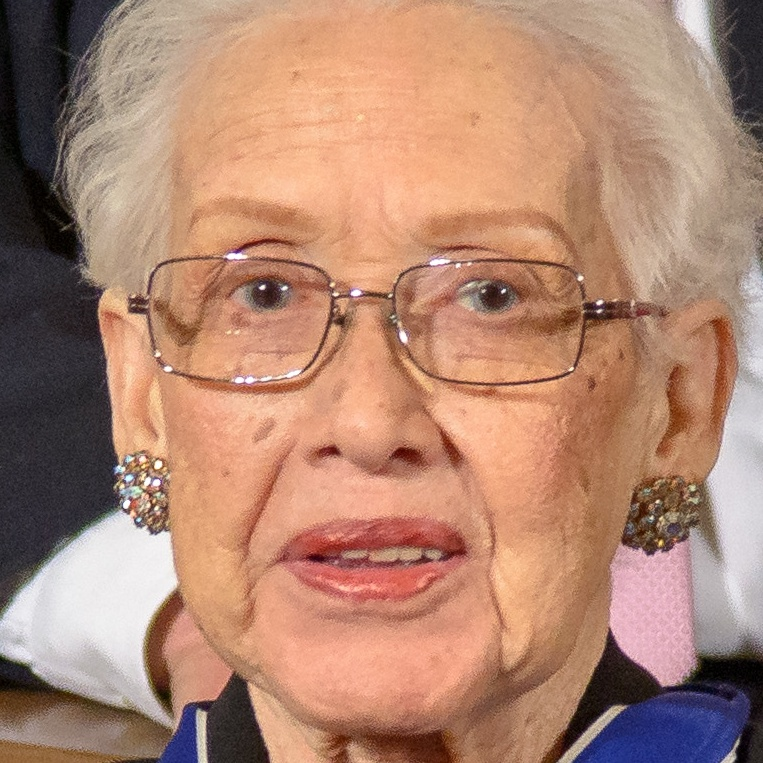
\includegraphics[width=5cm]{implementation/c.jpg} }}%
    \qquad
    \subfloat[Mask indicating skin pixels]{{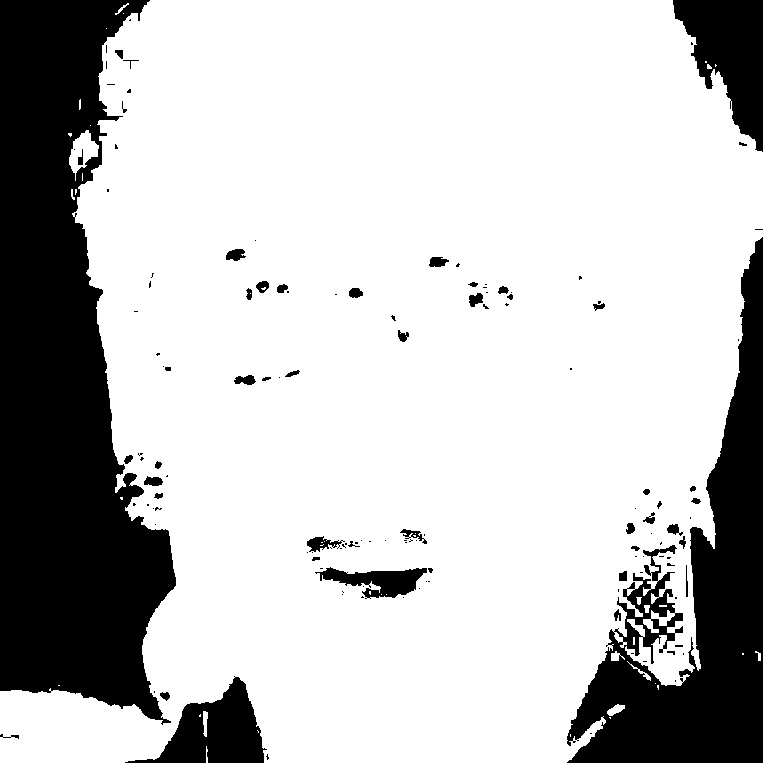
\includegraphics[width=5cm]{implementation/interval.jpg} }}%
   \caption{\textit{An example of the hair failure case}}
\end{figure}
% \footnotemark[1]
\footnotetext[1]{ An image of mathematician Katherine Johnson taken from the public domain.}
% EXPLAIN PERCEPTUAL UNIFORMITY 
% SHOW YCbCr REPRESENTATION OF SKIN PIXELS
% Talk about hair colour issue, doesn't work for lots of people, 
% Hence why we transition to figuring out skin tone
% crucially doesn't encode anything about the individual
%\subsection{Conditional Random Fields}

\subsubsection{K-Means}
If we consider how a human might identify skin, it could involve initially identifying the skin tone of the person and then assuming all parts of the face of a similar colour are in fact skin. This reduces the problem to identifying the skin tone in a face and then measuring the colour difference between each pixel and the skin tone. If the colours are within some specified threshold, then we can consider them to be skin pixels.
\\ \\
We might suppose that the image consists of clusters of pixels, some of which belong to the skin and others which don't. The center of the cluster of skin pixels represents the skin tone of the individual. Implicitly, this approach assumes that the Euclidean distance between points in our colour space is representative of the perceived colour difference. This property is known as perceptual uniformity and is not a property of all colour spaces. 
\\ \\
The colour space YCbCr is an approximation of perceptual uniformity and hence the image is converted from RGB before the application of clustering. 
% As a result, the colour space YCbCr happens to have this property and thus before any clustering is applied, the face image must be converted between these spaces. 
Under the assumption that our image consists of two clusters of pixels, skin and non-skin, we could simply apply 
the k-means algorithm\footnote{A popular algorithm for discovering clusters in data} \cite{kmeans}  identify these clusters of pixels. Under the further assumption that the majority of pixels 
are skin pixels, the largest cluster is returned as the set of skin pixels.

\begin{figure}[H]
    % Have an image from face to -> pixels in colour space on a graph with classification ->  to what classification looks like
    \centering
    \subfloat[Original image]{{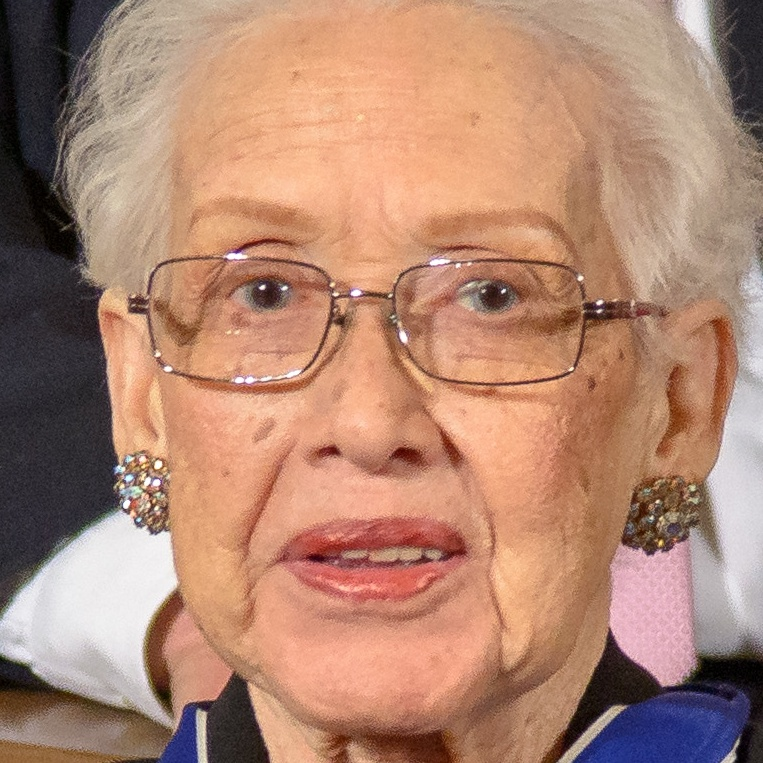
\includegraphics[width=5cm]{implementation/c.jpg} }}%
    \qquad
    \subfloat[Mask indicating regions considered to be skin.]{{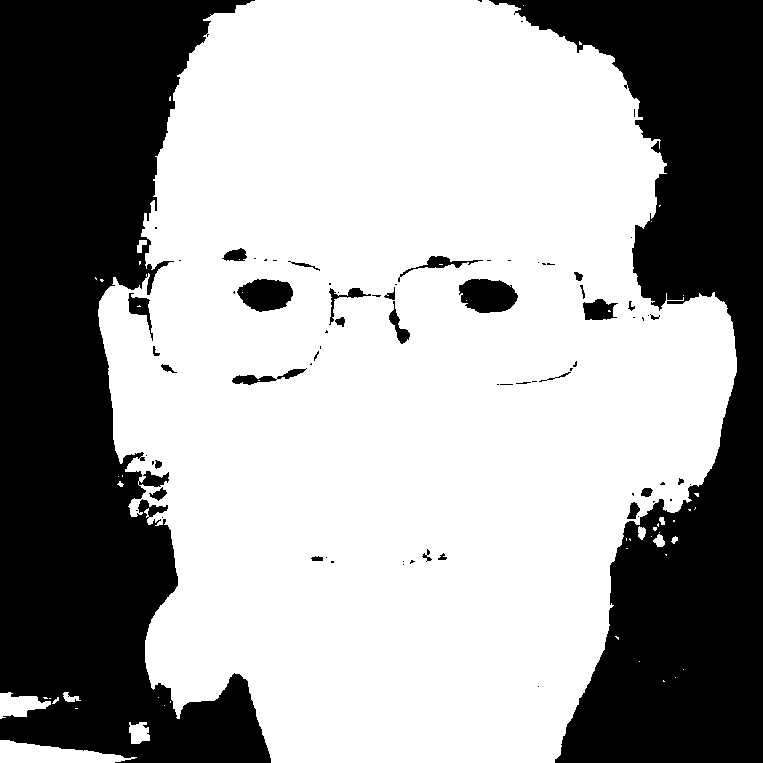
\includegraphics[width=5cm]{implementation/r2.jpg} }}%
    % \includegraphics[width=0.5\textwidth]{example-image-a}
   \caption{\textit{An example of the application of the k-means algorithm to skin detection}}
\end{figure}
%\subsubsection{Hierarchical clustering}
%\subsubsection{Markov clustering}
% \section{Ensemble Methods}


\paragraph{Issues}
\label{impl:kmeans_bad}
% Plethora of failure cases

%The four main issues: doesn't consider location of pixels, selecting k not trivial and can impact (GIVE AN EXAMPLE), complexity, illumination resistance

% Takes no consideration of relative location of pixels and shape information so could degenerate in scenarios 
% where for example, there's a wallpaper with similar skin colour to skin tone
% Should be able to deal with this by understanding that skin pixels will occur in large patches
% A small number of pixels which aren't in the cluster surrounded by pixels that are shouldn't be wiped out
% There's some notion of skin pixels amongst others should be considered skin pixels

% Selection of the number of clusters not obvious
% Just using 2 works well for backgrounds where it's a single colour or skin pixels are very close together
% Give an example where there's a really specific colour present in the background in a large quantity

% Breaks with shadows
% Illumination resistance is extremely difficult how is it possible to tell the difference between specular reflection and white eyeballs?
% Assumption of most pixels being skin fails
The k-means algorithm, although it improves on the results of the rudimentary approach has a plethora of pitfalls.
\begin{itemize}
    \item \textbf{Performance}: recall from Section \ref{section:system_design} that, since the region selection operates on every frame, it must run in real-time. However, in benchmarking the k-means reference implementation in the scikit-learn \cite{sklearn} library takes an order of magnitude longer than the minimum requirement for this constraint.\footnote{Suppose the camera streams at 30 frames per second, then each frame must be processed within 33ms, the reference implementation operates in the order of 100ms per frame. }.
    \item \textbf{Location}: since it encodes no notion of location with respect to other pixels, a lone pixel in the corner that has a similar colour to the skin tone is considered the same as a pixel surrounded by skin pixels.
    \item \textbf{Number of clusters}: there's no rigorous means for deciding the number of clusters to expect in the data and the selection of this value is critical. Too many clusters can cause unexpected behaviour, but too few can result in undesired pixels being considered. 
    \item \textbf{Illumination resistance}: the algorithm is not resistant to differences in illumination. For example, since there is no notion of location encoded, specular reflection on the forehead may not be considered as skin.
\end{itemize}

\begin{figure}[H]
    \centering
    % Have an image from face to -> pixels in colour space on a graph with classification ->  to what classification looks like
    % \includegraphics[width=0.5\textwidth]{example-image-a}
    \subfloat[Original image]{{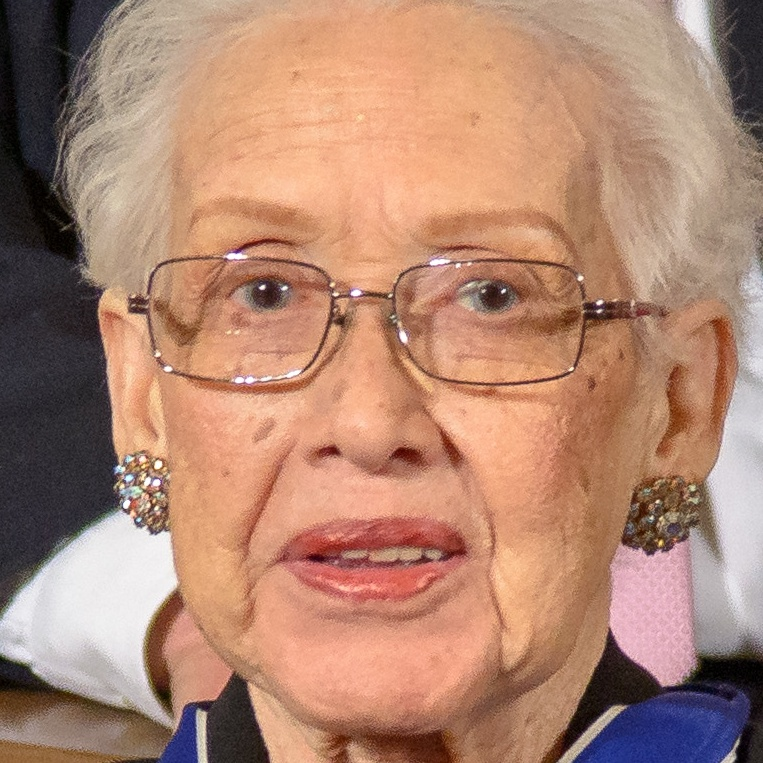
\includegraphics[width=3cm]{implementation/c.jpg} }}%
    \qquad
    \subfloat[Clustering w/ k=2]{{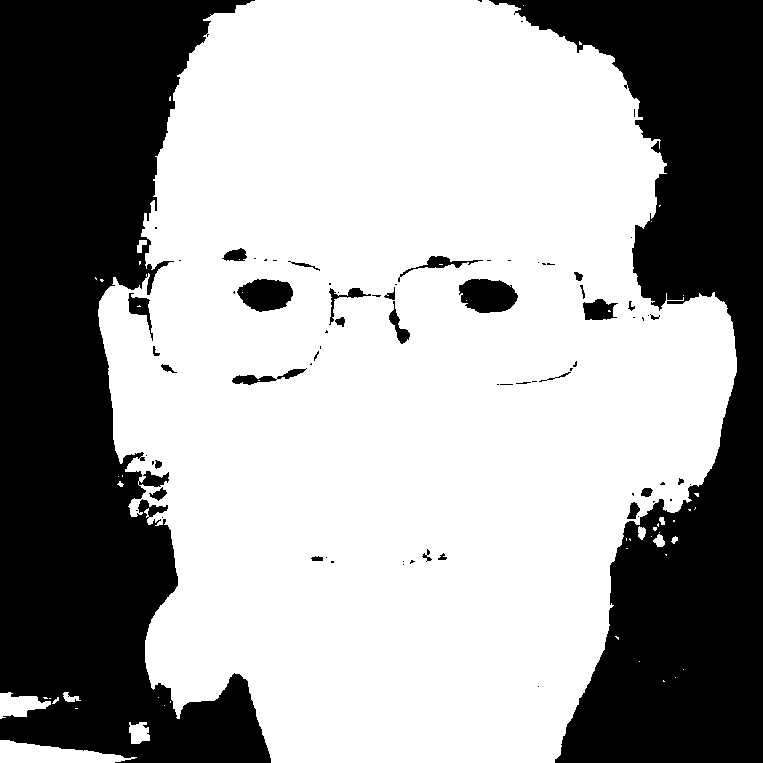
\includegraphics[width=3cm]{implementation/r2.jpg} }}%
    \qquad
    \subfloat[Clustering w/ k=3]{{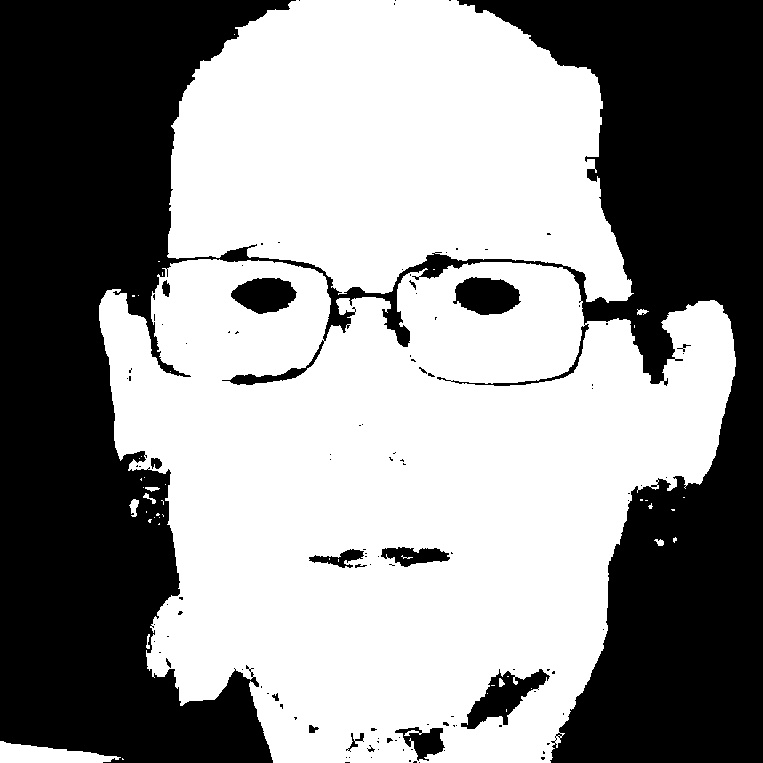
\includegraphics[width=3cm]{implementation/r3.jpg} }}%
    \qquad
    \subfloat[Clustering w/ k=4]{{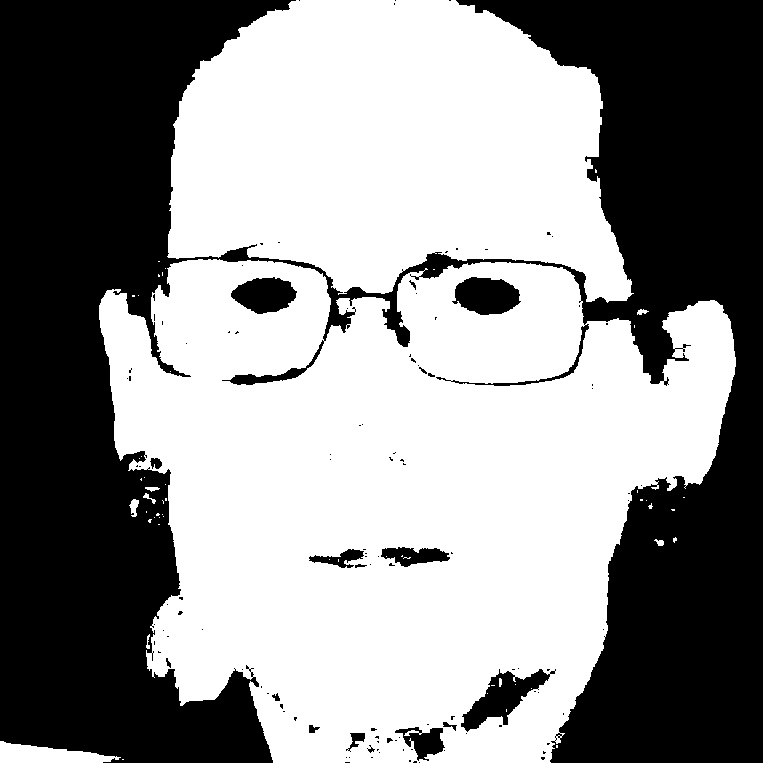
\includegraphics[width=3cm]{implementation/r4.jpg} }}%

    \subfloat[Original image\protect\footnotemark]{{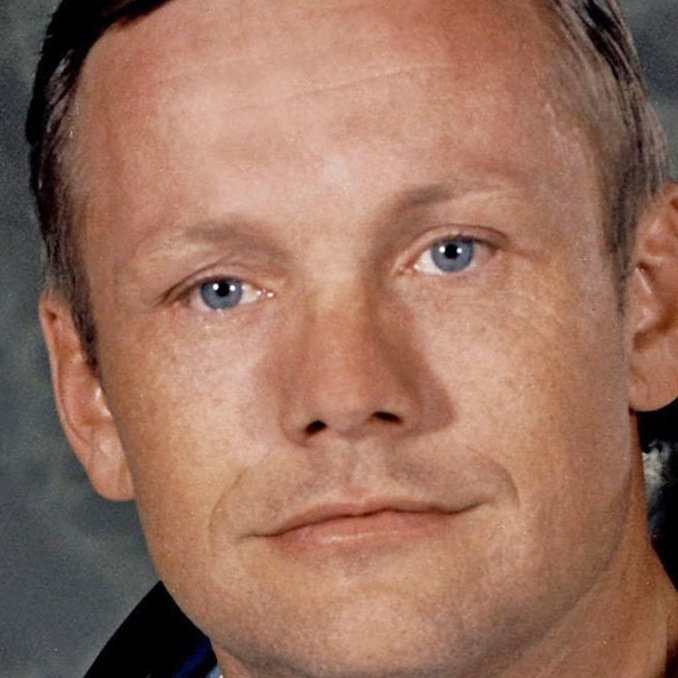
\includegraphics[width=3cm]{implementation/c-2.jpg} }}%
    \qquad
    \subfloat[Clustering w/ k=2]{{
\includegraphics[width=3cm]{implementation/r2-2.jpg} }}%
    \qquad
    \subfloat[Clustering w/ k=3]{{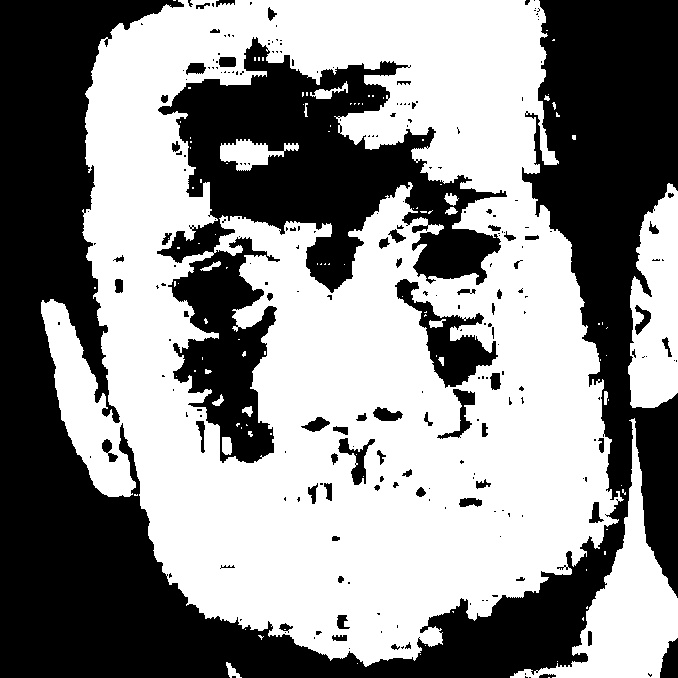
\includegraphics[width=3cm]{implementation/r3-2.jpg} }}%
    \qquad
    \subfloat[Clustering w/ k=4]{{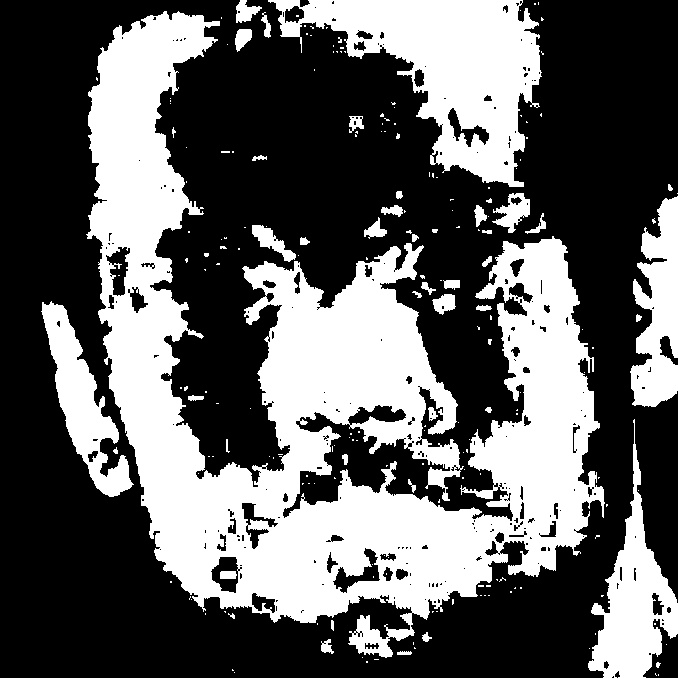
\includegraphics[width=3cm]{implementation/r4-2.jpg} }}%
   \caption{\textit{An example of the effect of differing the number of clusters} }
\end{figure}
\footnotetext[3]{An image of astronaut Neil Armstrong from the public domain. }
% \subparagraph{Complexity}
% Not practical to be run for real-time applications, as is one of the requirements outlined in the first section

\subsection{Improving the previous approaches}
Recall that the purpose of the region selection algorithm is to return the mean colour of the pixels considered. The mean value from each frame is taken as a time series which is used to infer the heart rate. So rather than attempting to classify each pixel as either skin or not, I use a combination of the previous techniques to take a weighted mean which emphasises pixels which are believed to be skin pixels, in such a way as to minimise the issues encountered with the previous techniques.
\\ \\
Instead of applying k-means to each frame, which is not feasible with the constraint of real-time performance, we apply it once at the start of the video.
One of the resulting clusters will correspond to the skin tone of the face in question.
Having identified the skin tone, this colour can be used as part of a probability model which we define to try and encode the likelihood of a particular pixel being part of the skin. 
In this way, we amortize the cost of skin detection over the entire video rather than per frame.
This reduces the problem to: 
\begin{itemize}
   \item Use k-means to identify the skin tone
   \item Use the skin tone to identify skin in the face for a large number of consecutive frames 
\end{itemize}
\subsubsection{Identifying the skin tone}
There are two expected properties of the cluster corresponding to the skin. It is likely to contain the largest number of pixels, since we'd expect most of the face to be composed of skin. It is also likely to fall within the range of expected human skin tones.
The difficulty of this problem, however, is that neither of these properties are guaranteed to hold.
For example, the face may be dominated by hair which could become the most prominent colour in the image. Likewise, changes in illumination or the presence of specular reflection might cause the skin tone of the face to be outside the expected range.
\\ \\
By considering both of these properties together, as a heuristic, it becomes more probable that the skin tone is identified correctly. I assign a score to each cluster, $C$, based on the number of elements in the cluster, $|C|$, and its distance from the expected range of skin tones, $d_C$.
\begin{equation*}
    \mathrm{score}(C) = \alpha\cdot |C| - \beta\cdot d_C
\end{equation*}
The constants $\alpha$ and $\beta$ were selected experimentally. The skin tone is identified as the center of the cluster with the maximum score.
% This is shown to improve on simply selecting the largest cluster in Section \ref{section:skin_tone_detection}.

\subsubsection{Identifying skin pixels using the skin tone}
Identifying the skin tone, as described, requires the use of the k-means algorithm,
however it is not particularly suitable for real-time applications (see Section \ref{impl:kmeans_bad}). Thus, the skin tone cannot be identified in every frame.
Given the skin tone from an earlier frame, the value must be used to robustly detect skin pixels in subsequent frames. This is challenging since there will almost certainly be changing illumination conditions as well as changing positions of the skin pixels.
\\ \\
% A possible approach could be to record the number of pixels that were in the skin cluster when the skin tone was identified. Then, our algorithm could select the $n$ closest pixels in the colour space to the skin tone, where $n$ was the number of pixels in the skin cluster. However, this would not be robust to rotations of the face, since, in subsequent frames, the number of pixels visible to the camera could change. Assuming a static value of $n$ would not be robust.
% \\ \\
Implicitly, the clustering approach relies on the assumption that any change in illumination between frames affects all pixels equally. 
It assumes that in subsequent frames, the true skin pixels remain closer (in terms of Euclidean distance) to the skin tone than the non-skin pixels.
%That is, the pixels which were within the skin cluster when k-means was applied, are still closer to the skin tone than non-skin pixels in subsequent frames. 
This is a fairly strong assumption and is affected by phenomena such as shadows and specular reflection, which do not affect all pixels equally.
However, it is useful enough to make the problem more tractable than it was previously, without undermining the fidelity of the algorithm. %if the skin tone is detected frequently enough. 
%The validity of this assumption is made clear by the evaluation of the algorithm presented in Section \ref{section:skin_tone_detection}.
% Therefore, we proceed by classifying pixels based on their Euclidean distance from the skin tone.
\\ \\
\paragraph{A Bayesian approach}
Recall that the first approach described classifies skin based on knowledge about the range of possible human skin tones. 
In this sense, it acts as a prior distribution; when classifying an individual pixel, it considers nothing of the face being presented.
The k-means implementation, on the other hand, considers the face presented but it has to knowledge of the prior. It instead assumes that the largest cluster must be the set of skin pixels.
\\ \\ 
A natural way to combine these two approaches would be to consider the problem of skin classification from a Bayesian perspective. Given some pixel $x_i$ we want to discover the likelihood of it being a skin pixel, having been conditionalised on the skin tone of the person as well the colour of the pixel being classified. 
We have access to the prior distribution from the first approach, which indicates the likelihood of a particular colour being skin.
Let us begin by denoting the following: 
\begin{itemize}
   \item $C_{\mathrm{skin}}$ the class of skin pixels
   \item $x_i$ the colour of the pixel being considered
   \item $s$ the skin tone of the face
\end{itemize} 
Given this notation the probability we wish to discover is the likelihood of a pixel being skin given its colour and the skin tone of the user.
\begin{equation*}
   \Pr(C_{\mathrm{skin}}| x_i, s) 
\end{equation*}
From Bayes' theorem, this can be re-written to expose the prior distribution.
\begin{align*}
   \frac{\Pr(C_\mathrm{skin}, x_i, s)}{\Pr(x_i, s)} = \frac{\Pr(s|C_\mathrm{skin}, x_i)\Pr(C_\mathrm{skin}|x_i)\Pr(x_i)}{\Pr(x_i,s)}
\end{align*}
% We could proceed with classification as follows, for some threshold probability $t$ that defines the decision boundary: 
% \begin{equation*}
%     \text{isSkin}(x_i) = 
%     \begin{cases}
%         \texttt{True}, \quad \text{if} \Pr(C_{\mathrm{skin}}| x_i, s) > t \\
%         \texttt{False}, \quad \text{otherwise}
%     \end{cases}
% \end{equation*}
% \begin{align*}
%     \Pr(C_\mathrm{skin}, x_i, s) &> \Pr(C_\mathrm{not-skin}, x_i, s) \\
%     \frac{\Pr(s|C_\mathrm{skin}, x_i)\Pr(C_\mathrm{skin}|x_i)\Pr(x_i)}{\Pr(x_i,s)} &> \frac{\Pr(s|C_\mathrm{not-skin}, x_i)\Pr(C_\mathrm{not-skin}|x_i)\Pr(x_i)}{\Pr(x_i,s)} \\
%     \Pr(s|C_\mathrm{skin}, x_i)\Pr(C_\mathrm{skin}|x_i) &> \Pr(s|C_\mathrm{not-skin}, x_i)\Pr(C_\mathrm{not-skin}|x_i) 
% \end{align*} 
% Since we're assuming that there are only two possible classes, this is equivalent to: 
% \begin{align*}
%     \Pr(s|C_\mathrm{skin}, x_i)\Pr(C_\mathrm{skin}|x_i) &> [1-\Pr(s|C_\mathrm{skin}, x_i)][1-\Pr(C_\mathrm{skin}|x_i)] \\
% \end{align*}
% So an equivalent condition in only a single class is: 
% \begin{equation*}
% \Pr(s|C_\mathrm{skin}, x_i)+\Pr(C_\mathrm{skin}|x_i) > 1
% \end{equation*}
% \Pr(s|C_\mathrm{skin}, x_i)\Pr(C_\mathrm{skin}|x_i) > t
\paragraph{Prior distribution}
Usually, one might attempt to learn the distributions $\Pr(C_\mathrm{skin}|x_i)$ and $\Pr(s|C_\mathrm{skin}, x_i)$ from  a relevant dataset.
The prior $\Pr(C_\mathrm{skin}|x_i)$ was computed as the empirical distribution from 
the dataset discussed in Section \ref{section:colour-filter}. This dataset consists of randomly sampled pixels that are classified as skin or not, it does not include entire classified faces.
Furthermore, to the best of my knowledge at the time of implementation, there are no publicly available, adequately sized datasets with this information. Hence, attempting to learn the distribution $\Pr(s|C_\mathrm{skin}, x_i)$ (denoted as the \textit{class conditional distribution} here) was not deemed to be feasible.
Once the distribution $\Pr(C_\mathrm{skin}|x_i,s)$ has been computed for a single frame, it is used as the prior for subsequent frames. This is for the purpose of providing greater resistance to 
sudden changes in the image.
and is a benefit of the Bayesian approach. It allows a principled means of incorporationg prior knowledge about the problem space.

\paragraph{Class conditional distribution}
A reasonable approach is to define the distribution $\Pr(s|C_\mathrm{skin}, x_i)$ based on the assumption that a skin pixel is likely close in colour to the overall skin tone. We want a function which returns a large probability if the Euclidean distance between the pixel and the skin tone is small.
There are, however, an infinite number of functions which could encode this. The only requirement is that the probability of being a skin pixel is decreasing as a function of the distance between the colour of the pixel and the skin tone of the face. 
\\\\
A reasonable assumption might be that if the pixel being considered, $x_i$, is a skin pixel, then the Euclidean distance between the skin tone, $s$ and the skin pixel, $d(s,x_i)$, varies as a Normal distribution with mean zero and standard deviation $\sigma$.
\begin{equation*}
   d(s, x_i) \sim N(0, \sigma) 
\end{equation*}
However, since colours are only represented in a finite interval, for example, between zero and one (or 0 and 255), this is not strictly correct. 
The above model has a non-zero probability associated with impossible colour values, since there are minimum and maximum possible distances.
As a result, I use a \textit{truncated} Normal distribution\footnote{A truncated distribution modifies the domain of a distribution by defining an updated probability density function which is zero outside a particular range $[a,b]$. This is achieved in such a way that the properties of a valid probability distribution are maintained.} instead.
\\\\
The probability density function of a truncated normal distribution between the values $a$ and $b$ and with mean, $\mu$, and variance, $\sigma$, is defined as: 
\begin{equation*}
    f(x) = \frac{1}{\sigma}\frac{\phi(\frac{x-\mu}{\sigma})}{\Phi(\frac{b-\mu}{\sigma}) - \Phi(\frac{a-\mu}{\sigma})}
\end{equation*}
\noindent
In this case, the values of $a$ and $b$ represent the minimum and maximum distances respectively from the given skin tone $s$. 
Hence, $a=0$, since the pixel being considered may have the same colour as the skin tone, in which case, $d(x_i, s) = d(s, s) = 0$.
The value of $b$ here is the distance between the skin tone and the furthest possible point in the colour space.
In this approach, a three dimensional colour space is used and, hence, the value of $b$ is the Euclidean distance between $s$ and the furthest corner of the colourspace cube.
\\\\
Given this, the probability is defined in proportion to the probability density function of the truncated distribution for each possible skin tone.
\begin{equation*}
    \Pr(s|C_\mathrm{skin}, x_i) = \frac{f(d(s,x_i))}{\sum_{s' \in C}f(d(s',x_i))}
\end{equation*}
\paragraph{Avoiding the need for thresholding}
The best choice of the threshold value is not obvious, but in this context, classification is not the goal.
The aim of the algorithm is to minimise the effect of non-skin pixels on the mean, so instead I proceed by taking a weighted 
mean colour based on the probability of each pixel being a skin pixel. 

\paragraph{Accelerating class conditional computation}
Computing the class-conditional distribution for each pixel in the bounding box of the face is a costly computation. 
The distribution defined is continuous in nature and so maintaining floating point accuracy means the distribution cannot be precomputed (with finite memory).
Instead, by, representing each component of the skin tone as an integer and rounding the Euclidean distance to the nearest integer, the distributions are precomputed 
for every possible skin tone. At runtime, the class conditional probability is achieved by lookup. Since the skin detection algorithm is applied to every frame in the video, 
using precomputed distributions achieves a 2x speedup in the overall pipeline (see Section \ref{eval:region_selection}).

\begin{figure}[H]
    \centering
    % Have an image from face to -> pixels in colour space on a graph with classification ->  to what classification looks like
    % \includegraphics[width=0.5\textwidth]{example-image-a}
    \subfloat[Original image]{{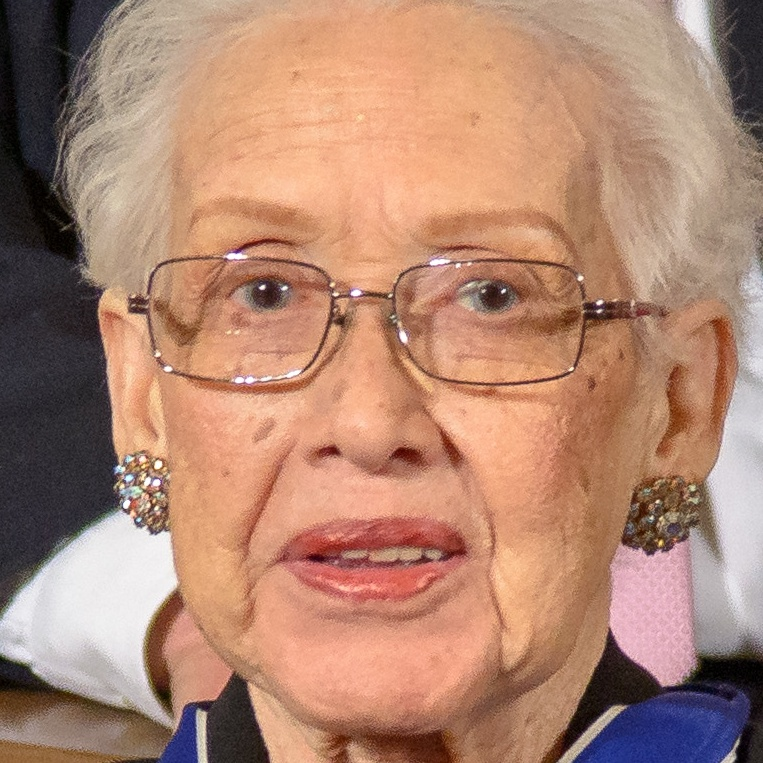
\includegraphics[width=4.9cm]{implementation/c.jpg} }}%
    \qquad
    \subfloat[Proposed]{{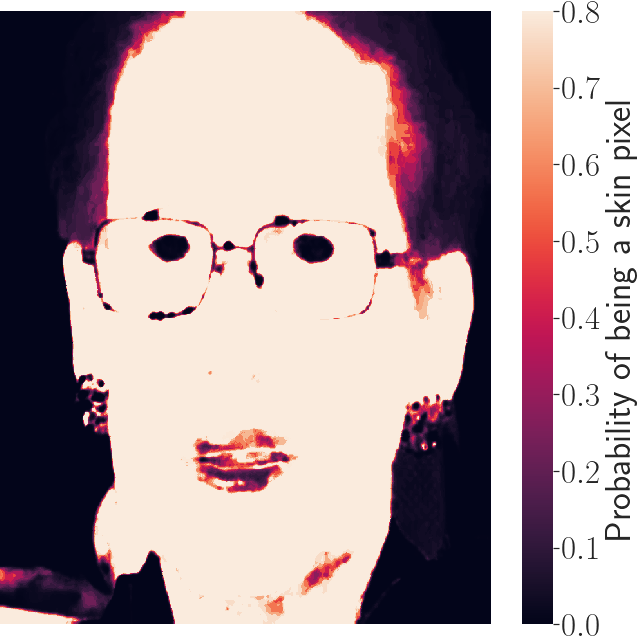
\includegraphics[width=5.2cm]{implementation/hmap-763-763.png} }}%

    \subfloat[Original image]{{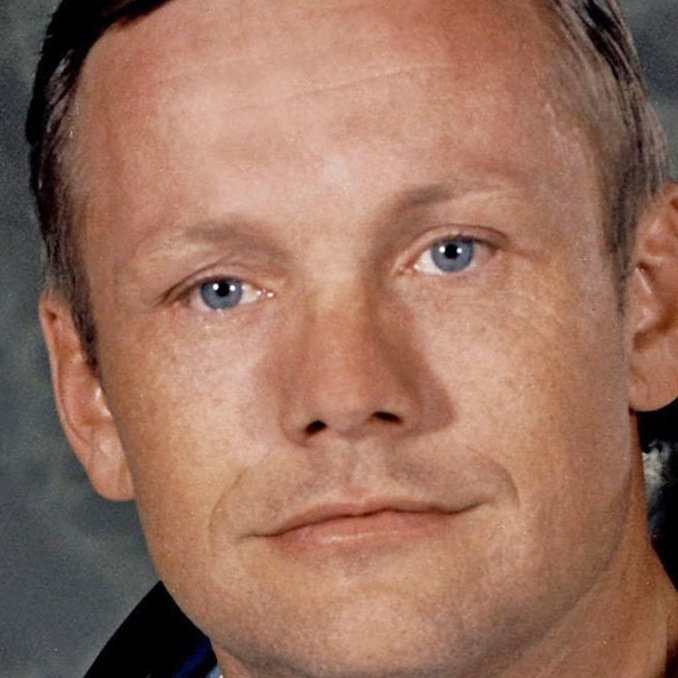
\includegraphics[width=4.9cm]{implementation/c-2.jpg} }}%
    \qquad
    \subfloat[Proposed]{{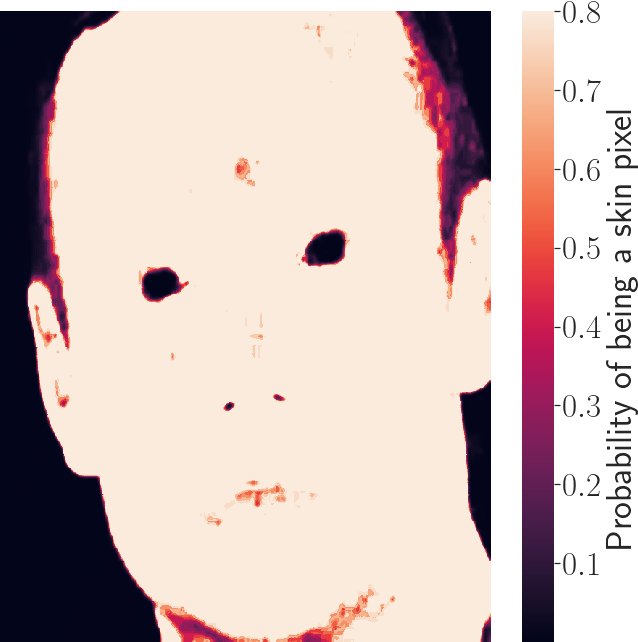
\includegraphics[width=5.2cm]{implementation/hmap-678-678.png} }}%
    % Give an example image with prior etc.
    % \includegraphics[width=0.5\textwidth]{example-image-b}
    % \input{implementation/test.pgf}
   \caption{\textit{An example result from the described skin detection algorithm} }
\end{figure}
\noindent
The approach described achieves similar results to applying k-means per frame, but at an amortized cost 
inversely proportional to the number of frames in the video. In practice, this results in a order of magnitude speedup in the time to process a frame
for videos with more than a single frame (see Appendix.). This means that skin detection is plausible whilst maintaining performance.


%Discrete or not??
% There is a finite range of possible values for the Euclidean distance between the colour of a pixel and the skin tone. This is because colours are discretised by the camera and therefore must lie between some set of bounds (usually 0 and 255). As a result, the defined distribution should also be discrete in nature.
% \\\\ 

 
% \begin{equation}
%    \Pr(C_{\mathrm{skin}}| x_i) = \Pr(C_{\mathrm{skin}}| x_i, \text{skin-tone} )\Pr(\text{skin-tone})
% \end{equation}


%I deem it to be a strong enough assumption to simply the problem adequately but not so strong as to undermine the effectiveness of the solution. 


% Describe how this addresses each of the problems

% Run multiple times with different k, and look for colours that repeat in each one to identify skin tone
% Use rudimentary filter to remove obviously wrong ones
% Consider cluster size

% TALK ABOUT COMPLEXITY OF K-MEANS AND WHY USING IT REPEATEDLY DOESN'T WORK THAT WELL
% Detect skin tone every x frames 
% Then define a probability distribution based on d

% Morphologies
% The rudimentary colour-filtering approach provides a good baseline as to the 










\section{Heart rate isolation}
% EXPLAIN WHY IT'S NOT JUST THE FOURIER POWER SPECTRUM
% IN VIDEOS WITH MOVEMENT WE EXPECT HEART RATE TO BE A SERIES OF PEAKS TOGETHER RATHER THAN A SINGLE PEAK
% THAT MIGHT BE DUE TO LIGHTING ETC
% IMPACT OF LIGHTING CONDITIONS
Given a time series of the mean colour in each frame, inferring the heart rate might, naively, be taken as the prevalent frequency. That is, the largest peak in the Fourier transform. 
However, it is important to consider that the colours observed are not only the result of the underlying biological phenomenon of interest. This naïve assumption is prone to returning, instead,
 the frequency of some other factor that impacts colour of the face. For example, respiration or movement of the face will have an impact, as well as any repetitive changes in lighting such as flickering. 
 Isolating the heart rate signal from the observed colour of the face, is a key part of the project.
\\\\
To simplify this approach the problem is broken down into two subtasks:
\begin{itemize}
    \item Identifying the pulse signal: given the noisy time series of observed colours for each frame, identify the signal corresponding to the pulse of the user
    \item Identifying the heart rate: given the pulse signal, identify the heart rate
\end{itemize}
Although, as will be explained, there is some overlap between the two to aid with correctly identifying the pulse.

\subsection{Blind-source separation}
\label{implementation:pca_ica}
Suppose that our observed colour signal, $\mathbf{I}(t)$, a vector-valued function, consists of a mixture of several underlying signals, $x_i(t)$ one of which is the pulse, $p(t)$. 
Our observed signal exists in three dimensions and can be viewed as the result of the mixing of three underlying signals by some mixing matrix $\mathbf{A}$.
\begin{equation*}
    \mathbf{I}(t) = \mathbf{A}\begin{bmatrix} x_1(t) \\ x_2(t) \\ x_3(t) \end{bmatrix}
\end{equation*}
% If we consider $\mathbf{I}(t)$ as a matrix of dimension $n \times T$ where $n$ is the number of colour dimensions and $T$ the number of timesteps, then we might suppose that $ (x_1(t), x_2(t), ..., p(t), ..., x_{n-1}(t))^T = AI$. That is 
% That is: $\mathbf{I}(t) = (x_1(t), x_2(t), x_3(t))$, for constants $\lambda_i$. 
% Alternatively we can consider this as finding the set of basis vectors $v_1, v_2, v_3$ such that $I(t) = (I(t)\cdot v_1)v_1 + (I(t) \cdot v_2)v_2 + (I(t) \cdot v_3)v_3$. The key problem is finding the basis $v_1, v_2, v_3$ such that $p(t) = (I(t)\cdot v_i))v_i$ for some $i$ and further identifying the value of $i$.
The nature of this task is to identify and return $p(t)$ from only $\mathbf{I}(t)$ and is known as the blind-source separation problem see (Section \ref{ref:bss_prep}).
The above formulation is not enough to isolate the signal $p(t)$ from $\mathbf{I}(t)$ and  so assumptions must be placed on the nature of each $x_i(t)$ and $p(t)$ in order 
to solve this.
% \\ \\ 
% We can reframe this as finding some basis for our vector space $I(t) = \sum_{i}^{n}I(t)\cdot(v_i)v_i$

\subsubsection{Independent component analysis (ICA)}
A possible assumption might be that each of the $x_i(t)$ are statistically independent. 
That is, informally, one cannot gain any information about one of these signals given another. 
This assumption encodes the notion that the pulse should be entirely independent from the other phenomena impacting the observed signal.
\\\\
For example, suppose that some of the $x_i(t)$ are the result of a physical phenomenon such as lighting conditions. In this case, it is intuitive to expect there to be no mutual information between the pulse and the other constituent signals. The ICA algorithm \cite{ica} attempts to identify these signals based on this assumption, by using non-Gaussianity as a proxy for statistical independence.
\\\\
% talk about how this doesn't tell us which one is p(t) 
Crucially, however, this approach returns the signals $x_1(t)$, $x_2(t)$ and $x_3(t)$ but gives no indication regarding which signal corresponds to the pulse. In fact, the formulation of the ICA algorithm is such that each $x_i(t)$ are returned in a random order. Additional work must be undertaken to identify the pulse from the returned signal. 
\\\\
I proceed by attempting to identify the heart rate in each of these signals independently. This results in returning three different heart rate values, each of which has an associated power.
This power value, which is the magnitude of the term in the Fourier transform associated with a given frequency, acts as a natural way of quantifying the importance of a particular frequency on the overall signal.
\begin{figure}[H]
    \centering
    \subfloat[\textit{Raw video signal}]{\scalebox{0.43}{%% Creator: Matplotlib, PGF backend
%%
%% To include the figure in your LaTeX document, write
%%   \input{<filename>.pgf}
%%
%% Make sure the required packages are loaded in your preamble
%%   \usepackage{pgf}
%%
%% and, on pdftex
%%   \usepackage[utf8]{inputenc}\DeclareUnicodeCharacter{2212}{-}
%%
%% or, on luatex and xetex
%%   \usepackage{unicode-math}
%%
%% Figures using additional raster images can only be included by \input if
%% they are in the same directory as the main LaTeX file. For loading figures
%% from other directories you can use the `import` package
%%   \usepackage{import}
%%
%% and then include the figures with
%%   \import{<path to file>}{<filename>.pgf}
%%
%% Matplotlib used the following preamble
%%   \usepackage{fontspec}
%%   \setmainfont{DejaVuSerif.ttf}[Path=/Users/yousuf/Library/Python/3.7/lib/python/site-packages/matplotlib/mpl-data/fonts/ttf/]
%%   \setsansfont{DejaVuSans.ttf}[Path=/Users/yousuf/Library/Python/3.7/lib/python/site-packages/matplotlib/mpl-data/fonts/ttf/]
%%   \setmonofont{DejaVuSansMono.ttf}[Path=/Users/yousuf/Library/Python/3.7/lib/python/site-packages/matplotlib/mpl-data/fonts/ttf/]
%%
\begingroup%
\makeatletter%
\begin{pgfpicture}%
\pgfpathrectangle{\pgfpointorigin}{\pgfqpoint{4.000000in}{3.000000in}}%
\pgfusepath{use as bounding box, clip}%
\begin{pgfscope}%
\pgfsetbuttcap%
\pgfsetmiterjoin%
\definecolor{currentfill}{rgb}{1.000000,1.000000,1.000000}%
\pgfsetfillcolor{currentfill}%
\pgfsetlinewidth{0.000000pt}%
\definecolor{currentstroke}{rgb}{1.000000,1.000000,1.000000}%
\pgfsetstrokecolor{currentstroke}%
\pgfsetdash{}{0pt}%
\pgfpathmoveto{\pgfqpoint{0.000000in}{0.000000in}}%
\pgfpathlineto{\pgfqpoint{4.000000in}{0.000000in}}%
\pgfpathlineto{\pgfqpoint{4.000000in}{3.000000in}}%
\pgfpathlineto{\pgfqpoint{0.000000in}{3.000000in}}%
\pgfpathclose%
\pgfusepath{fill}%
\end{pgfscope}%
\begin{pgfscope}%
\pgfsetbuttcap%
\pgfsetmiterjoin%
\definecolor{currentfill}{rgb}{1.000000,1.000000,1.000000}%
\pgfsetfillcolor{currentfill}%
\pgfsetlinewidth{0.000000pt}%
\definecolor{currentstroke}{rgb}{0.000000,0.000000,0.000000}%
\pgfsetstrokecolor{currentstroke}%
\pgfsetstrokeopacity{0.000000}%
\pgfsetdash{}{0pt}%
\pgfpathmoveto{\pgfqpoint{0.511111in}{0.580556in}}%
\pgfpathlineto{\pgfqpoint{3.850000in}{0.580556in}}%
\pgfpathlineto{\pgfqpoint{3.850000in}{2.850000in}}%
\pgfpathlineto{\pgfqpoint{0.511111in}{2.850000in}}%
\pgfpathclose%
\pgfusepath{fill}%
\end{pgfscope}%
\begin{pgfscope}%
\pgfsetbuttcap%
\pgfsetroundjoin%
\definecolor{currentfill}{rgb}{0.000000,0.000000,0.000000}%
\pgfsetfillcolor{currentfill}%
\pgfsetlinewidth{0.803000pt}%
\definecolor{currentstroke}{rgb}{0.000000,0.000000,0.000000}%
\pgfsetstrokecolor{currentstroke}%
\pgfsetdash{}{0pt}%
\pgfsys@defobject{currentmarker}{\pgfqpoint{0.000000in}{-0.048611in}}{\pgfqpoint{0.000000in}{0.000000in}}{%
\pgfpathmoveto{\pgfqpoint{0.000000in}{0.000000in}}%
\pgfpathlineto{\pgfqpoint{0.000000in}{-0.048611in}}%
\pgfusepath{stroke,fill}%
}%
\begin{pgfscope}%
\pgfsys@transformshift{0.662879in}{0.580556in}%
\pgfsys@useobject{currentmarker}{}%
\end{pgfscope}%
\end{pgfscope}%
\begin{pgfscope}%
\definecolor{textcolor}{rgb}{0.000000,0.000000,0.000000}%
\pgfsetstrokecolor{textcolor}%
\pgfsetfillcolor{textcolor}%
\pgftext[x=0.662879in,y=0.483333in,,top]{\color{textcolor}\sffamily\fontsize{10.000000}{12.000000}\selectfont 0}%
\end{pgfscope}%
\begin{pgfscope}%
\pgfsetbuttcap%
\pgfsetroundjoin%
\definecolor{currentfill}{rgb}{0.000000,0.000000,0.000000}%
\pgfsetfillcolor{currentfill}%
\pgfsetlinewidth{0.803000pt}%
\definecolor{currentstroke}{rgb}{0.000000,0.000000,0.000000}%
\pgfsetstrokecolor{currentstroke}%
\pgfsetdash{}{0pt}%
\pgfsys@defobject{currentmarker}{\pgfqpoint{0.000000in}{-0.048611in}}{\pgfqpoint{0.000000in}{0.000000in}}{%
\pgfpathmoveto{\pgfqpoint{0.000000in}{0.000000in}}%
\pgfpathlineto{\pgfqpoint{0.000000in}{-0.048611in}}%
\pgfusepath{stroke,fill}%
}%
\begin{pgfscope}%
\pgfsys@transformshift{1.271980in}{0.580556in}%
\pgfsys@useobject{currentmarker}{}%
\end{pgfscope}%
\end{pgfscope}%
\begin{pgfscope}%
\definecolor{textcolor}{rgb}{0.000000,0.000000,0.000000}%
\pgfsetstrokecolor{textcolor}%
\pgfsetfillcolor{textcolor}%
\pgftext[x=1.271980in,y=0.483333in,,top]{\color{textcolor}\sffamily\fontsize{10.000000}{12.000000}\selectfont 2}%
\end{pgfscope}%
\begin{pgfscope}%
\pgfsetbuttcap%
\pgfsetroundjoin%
\definecolor{currentfill}{rgb}{0.000000,0.000000,0.000000}%
\pgfsetfillcolor{currentfill}%
\pgfsetlinewidth{0.803000pt}%
\definecolor{currentstroke}{rgb}{0.000000,0.000000,0.000000}%
\pgfsetstrokecolor{currentstroke}%
\pgfsetdash{}{0pt}%
\pgfsys@defobject{currentmarker}{\pgfqpoint{0.000000in}{-0.048611in}}{\pgfqpoint{0.000000in}{0.000000in}}{%
\pgfpathmoveto{\pgfqpoint{0.000000in}{0.000000in}}%
\pgfpathlineto{\pgfqpoint{0.000000in}{-0.048611in}}%
\pgfusepath{stroke,fill}%
}%
\begin{pgfscope}%
\pgfsys@transformshift{1.881081in}{0.580556in}%
\pgfsys@useobject{currentmarker}{}%
\end{pgfscope}%
\end{pgfscope}%
\begin{pgfscope}%
\definecolor{textcolor}{rgb}{0.000000,0.000000,0.000000}%
\pgfsetstrokecolor{textcolor}%
\pgfsetfillcolor{textcolor}%
\pgftext[x=1.881081in,y=0.483333in,,top]{\color{textcolor}\sffamily\fontsize{10.000000}{12.000000}\selectfont 4}%
\end{pgfscope}%
\begin{pgfscope}%
\pgfsetbuttcap%
\pgfsetroundjoin%
\definecolor{currentfill}{rgb}{0.000000,0.000000,0.000000}%
\pgfsetfillcolor{currentfill}%
\pgfsetlinewidth{0.803000pt}%
\definecolor{currentstroke}{rgb}{0.000000,0.000000,0.000000}%
\pgfsetstrokecolor{currentstroke}%
\pgfsetdash{}{0pt}%
\pgfsys@defobject{currentmarker}{\pgfqpoint{0.000000in}{-0.048611in}}{\pgfqpoint{0.000000in}{0.000000in}}{%
\pgfpathmoveto{\pgfqpoint{0.000000in}{0.000000in}}%
\pgfpathlineto{\pgfqpoint{0.000000in}{-0.048611in}}%
\pgfusepath{stroke,fill}%
}%
\begin{pgfscope}%
\pgfsys@transformshift{2.490182in}{0.580556in}%
\pgfsys@useobject{currentmarker}{}%
\end{pgfscope}%
\end{pgfscope}%
\begin{pgfscope}%
\definecolor{textcolor}{rgb}{0.000000,0.000000,0.000000}%
\pgfsetstrokecolor{textcolor}%
\pgfsetfillcolor{textcolor}%
\pgftext[x=2.490182in,y=0.483333in,,top]{\color{textcolor}\sffamily\fontsize{10.000000}{12.000000}\selectfont 6}%
\end{pgfscope}%
\begin{pgfscope}%
\pgfsetbuttcap%
\pgfsetroundjoin%
\definecolor{currentfill}{rgb}{0.000000,0.000000,0.000000}%
\pgfsetfillcolor{currentfill}%
\pgfsetlinewidth{0.803000pt}%
\definecolor{currentstroke}{rgb}{0.000000,0.000000,0.000000}%
\pgfsetstrokecolor{currentstroke}%
\pgfsetdash{}{0pt}%
\pgfsys@defobject{currentmarker}{\pgfqpoint{0.000000in}{-0.048611in}}{\pgfqpoint{0.000000in}{0.000000in}}{%
\pgfpathmoveto{\pgfqpoint{0.000000in}{0.000000in}}%
\pgfpathlineto{\pgfqpoint{0.000000in}{-0.048611in}}%
\pgfusepath{stroke,fill}%
}%
\begin{pgfscope}%
\pgfsys@transformshift{3.099283in}{0.580556in}%
\pgfsys@useobject{currentmarker}{}%
\end{pgfscope}%
\end{pgfscope}%
\begin{pgfscope}%
\definecolor{textcolor}{rgb}{0.000000,0.000000,0.000000}%
\pgfsetstrokecolor{textcolor}%
\pgfsetfillcolor{textcolor}%
\pgftext[x=3.099283in,y=0.483333in,,top]{\color{textcolor}\sffamily\fontsize{10.000000}{12.000000}\selectfont 8}%
\end{pgfscope}%
\begin{pgfscope}%
\pgfsetbuttcap%
\pgfsetroundjoin%
\definecolor{currentfill}{rgb}{0.000000,0.000000,0.000000}%
\pgfsetfillcolor{currentfill}%
\pgfsetlinewidth{0.803000pt}%
\definecolor{currentstroke}{rgb}{0.000000,0.000000,0.000000}%
\pgfsetstrokecolor{currentstroke}%
\pgfsetdash{}{0pt}%
\pgfsys@defobject{currentmarker}{\pgfqpoint{0.000000in}{-0.048611in}}{\pgfqpoint{0.000000in}{0.000000in}}{%
\pgfpathmoveto{\pgfqpoint{0.000000in}{0.000000in}}%
\pgfpathlineto{\pgfqpoint{0.000000in}{-0.048611in}}%
\pgfusepath{stroke,fill}%
}%
\begin{pgfscope}%
\pgfsys@transformshift{3.708384in}{0.580556in}%
\pgfsys@useobject{currentmarker}{}%
\end{pgfscope}%
\end{pgfscope}%
\begin{pgfscope}%
\definecolor{textcolor}{rgb}{0.000000,0.000000,0.000000}%
\pgfsetstrokecolor{textcolor}%
\pgfsetfillcolor{textcolor}%
\pgftext[x=3.708384in,y=0.483333in,,top]{\color{textcolor}\sffamily\fontsize{10.000000}{12.000000}\selectfont 10}%
\end{pgfscope}%
\begin{pgfscope}%
\definecolor{textcolor}{rgb}{0.000000,0.000000,0.000000}%
\pgfsetstrokecolor{textcolor}%
\pgfsetfillcolor{textcolor}%
\pgftext[x=2.180556in,y=0.293365in,,top]{\color{textcolor}\sffamily\fontsize{10.000000}{12.000000}\selectfont Time (s)}%
\end{pgfscope}%
\begin{pgfscope}%
\pgfsetbuttcap%
\pgfsetroundjoin%
\definecolor{currentfill}{rgb}{0.000000,0.000000,0.000000}%
\pgfsetfillcolor{currentfill}%
\pgfsetlinewidth{0.803000pt}%
\definecolor{currentstroke}{rgb}{0.000000,0.000000,0.000000}%
\pgfsetstrokecolor{currentstroke}%
\pgfsetdash{}{0pt}%
\pgfsys@defobject{currentmarker}{\pgfqpoint{-0.048611in}{0.000000in}}{\pgfqpoint{0.000000in}{0.000000in}}{%
\pgfpathmoveto{\pgfqpoint{0.000000in}{0.000000in}}%
\pgfpathlineto{\pgfqpoint{-0.048611in}{0.000000in}}%
\pgfusepath{stroke,fill}%
}%
\begin{pgfscope}%
\pgfsys@transformshift{0.511111in}{0.709068in}%
\pgfsys@useobject{currentmarker}{}%
\end{pgfscope}%
\end{pgfscope}%
\begin{pgfscope}%
\definecolor{textcolor}{rgb}{0.000000,0.000000,0.000000}%
\pgfsetstrokecolor{textcolor}%
\pgfsetfillcolor{textcolor}%
\pgftext[x=0.237158in, y=0.656306in, left, base]{\color{textcolor}\sffamily\fontsize{10.000000}{12.000000}\selectfont 80}%
\end{pgfscope}%
\begin{pgfscope}%
\pgfsetbuttcap%
\pgfsetroundjoin%
\definecolor{currentfill}{rgb}{0.000000,0.000000,0.000000}%
\pgfsetfillcolor{currentfill}%
\pgfsetlinewidth{0.803000pt}%
\definecolor{currentstroke}{rgb}{0.000000,0.000000,0.000000}%
\pgfsetstrokecolor{currentstroke}%
\pgfsetdash{}{0pt}%
\pgfsys@defobject{currentmarker}{\pgfqpoint{-0.048611in}{0.000000in}}{\pgfqpoint{0.000000in}{0.000000in}}{%
\pgfpathmoveto{\pgfqpoint{0.000000in}{0.000000in}}%
\pgfpathlineto{\pgfqpoint{-0.048611in}{0.000000in}}%
\pgfusepath{stroke,fill}%
}%
\begin{pgfscope}%
\pgfsys@transformshift{0.511111in}{1.227982in}%
\pgfsys@useobject{currentmarker}{}%
\end{pgfscope}%
\end{pgfscope}%
\begin{pgfscope}%
\definecolor{textcolor}{rgb}{0.000000,0.000000,0.000000}%
\pgfsetstrokecolor{textcolor}%
\pgfsetfillcolor{textcolor}%
\pgftext[x=0.148793in, y=1.175221in, left, base]{\color{textcolor}\sffamily\fontsize{10.000000}{12.000000}\selectfont 100}%
\end{pgfscope}%
\begin{pgfscope}%
\pgfsetbuttcap%
\pgfsetroundjoin%
\definecolor{currentfill}{rgb}{0.000000,0.000000,0.000000}%
\pgfsetfillcolor{currentfill}%
\pgfsetlinewidth{0.803000pt}%
\definecolor{currentstroke}{rgb}{0.000000,0.000000,0.000000}%
\pgfsetstrokecolor{currentstroke}%
\pgfsetdash{}{0pt}%
\pgfsys@defobject{currentmarker}{\pgfqpoint{-0.048611in}{0.000000in}}{\pgfqpoint{0.000000in}{0.000000in}}{%
\pgfpathmoveto{\pgfqpoint{0.000000in}{0.000000in}}%
\pgfpathlineto{\pgfqpoint{-0.048611in}{0.000000in}}%
\pgfusepath{stroke,fill}%
}%
\begin{pgfscope}%
\pgfsys@transformshift{0.511111in}{1.746897in}%
\pgfsys@useobject{currentmarker}{}%
\end{pgfscope}%
\end{pgfscope}%
\begin{pgfscope}%
\definecolor{textcolor}{rgb}{0.000000,0.000000,0.000000}%
\pgfsetstrokecolor{textcolor}%
\pgfsetfillcolor{textcolor}%
\pgftext[x=0.148793in, y=1.694135in, left, base]{\color{textcolor}\sffamily\fontsize{10.000000}{12.000000}\selectfont 120}%
\end{pgfscope}%
\begin{pgfscope}%
\pgfsetbuttcap%
\pgfsetroundjoin%
\definecolor{currentfill}{rgb}{0.000000,0.000000,0.000000}%
\pgfsetfillcolor{currentfill}%
\pgfsetlinewidth{0.803000pt}%
\definecolor{currentstroke}{rgb}{0.000000,0.000000,0.000000}%
\pgfsetstrokecolor{currentstroke}%
\pgfsetdash{}{0pt}%
\pgfsys@defobject{currentmarker}{\pgfqpoint{-0.048611in}{0.000000in}}{\pgfqpoint{0.000000in}{0.000000in}}{%
\pgfpathmoveto{\pgfqpoint{0.000000in}{0.000000in}}%
\pgfpathlineto{\pgfqpoint{-0.048611in}{0.000000in}}%
\pgfusepath{stroke,fill}%
}%
\begin{pgfscope}%
\pgfsys@transformshift{0.511111in}{2.265811in}%
\pgfsys@useobject{currentmarker}{}%
\end{pgfscope}%
\end{pgfscope}%
\begin{pgfscope}%
\definecolor{textcolor}{rgb}{0.000000,0.000000,0.000000}%
\pgfsetstrokecolor{textcolor}%
\pgfsetfillcolor{textcolor}%
\pgftext[x=0.148793in, y=2.213050in, left, base]{\color{textcolor}\sffamily\fontsize{10.000000}{12.000000}\selectfont 140}%
\end{pgfscope}%
\begin{pgfscope}%
\pgfsetbuttcap%
\pgfsetroundjoin%
\definecolor{currentfill}{rgb}{0.000000,0.000000,0.000000}%
\pgfsetfillcolor{currentfill}%
\pgfsetlinewidth{0.803000pt}%
\definecolor{currentstroke}{rgb}{0.000000,0.000000,0.000000}%
\pgfsetstrokecolor{currentstroke}%
\pgfsetdash{}{0pt}%
\pgfsys@defobject{currentmarker}{\pgfqpoint{-0.048611in}{0.000000in}}{\pgfqpoint{0.000000in}{0.000000in}}{%
\pgfpathmoveto{\pgfqpoint{0.000000in}{0.000000in}}%
\pgfpathlineto{\pgfqpoint{-0.048611in}{0.000000in}}%
\pgfusepath{stroke,fill}%
}%
\begin{pgfscope}%
\pgfsys@transformshift{0.511111in}{2.784725in}%
\pgfsys@useobject{currentmarker}{}%
\end{pgfscope}%
\end{pgfscope}%
\begin{pgfscope}%
\definecolor{textcolor}{rgb}{0.000000,0.000000,0.000000}%
\pgfsetstrokecolor{textcolor}%
\pgfsetfillcolor{textcolor}%
\pgftext[x=0.148793in, y=2.731964in, left, base]{\color{textcolor}\sffamily\fontsize{10.000000}{12.000000}\selectfont 160}%
\end{pgfscope}%
\begin{pgfscope}%
\pgfpathrectangle{\pgfqpoint{0.511111in}{0.580556in}}{\pgfqpoint{3.338889in}{2.269444in}}%
\pgfusepath{clip}%
\pgfsetrectcap%
\pgfsetroundjoin%
\pgfsetlinewidth{1.505625pt}%
\definecolor{currentstroke}{rgb}{1.000000,0.000000,0.000000}%
\pgfsetstrokecolor{currentstroke}%
\pgfsetdash{}{0pt}%
\pgfpathmoveto{\pgfqpoint{0.662879in}{0.778337in}}%
\pgfpathlineto{\pgfqpoint{0.673030in}{0.775523in}}%
\pgfpathlineto{\pgfqpoint{0.683182in}{0.798094in}}%
\pgfpathlineto{\pgfqpoint{0.693334in}{0.765644in}}%
\pgfpathlineto{\pgfqpoint{0.703486in}{0.777147in}}%
\pgfpathlineto{\pgfqpoint{0.713637in}{0.770791in}}%
\pgfpathlineto{\pgfqpoint{0.723789in}{0.812767in}}%
\pgfpathlineto{\pgfqpoint{0.733941in}{0.823441in}}%
\pgfpathlineto{\pgfqpoint{0.744092in}{0.856625in}}%
\pgfpathlineto{\pgfqpoint{0.754244in}{0.877345in}}%
\pgfpathlineto{\pgfqpoint{0.764396in}{0.863539in}}%
\pgfpathlineto{\pgfqpoint{0.774547in}{0.874410in}}%
\pgfpathlineto{\pgfqpoint{0.784699in}{0.853205in}}%
\pgfpathlineto{\pgfqpoint{0.794851in}{0.820611in}}%
\pgfpathlineto{\pgfqpoint{0.805002in}{0.775370in}}%
\pgfpathlineto{\pgfqpoint{0.815154in}{0.746118in}}%
\pgfpathlineto{\pgfqpoint{0.825306in}{0.758514in}}%
\pgfpathlineto{\pgfqpoint{0.835457in}{0.792681in}}%
\pgfpathlineto{\pgfqpoint{0.855761in}{0.785293in}}%
\pgfpathlineto{\pgfqpoint{0.865912in}{0.762880in}}%
\pgfpathlineto{\pgfqpoint{0.876064in}{0.808671in}}%
\pgfpathlineto{\pgfqpoint{0.886216in}{0.785652in}}%
\pgfpathlineto{\pgfqpoint{0.896368in}{0.736958in}}%
\pgfpathlineto{\pgfqpoint{0.906519in}{0.697888in}}%
\pgfpathlineto{\pgfqpoint{0.916671in}{0.728707in}}%
\pgfpathlineto{\pgfqpoint{0.926823in}{0.775467in}}%
\pgfpathlineto{\pgfqpoint{0.936974in}{0.789991in}}%
\pgfpathlineto{\pgfqpoint{0.947126in}{0.808627in}}%
\pgfpathlineto{\pgfqpoint{0.957278in}{0.784711in}}%
\pgfpathlineto{\pgfqpoint{0.967429in}{0.800385in}}%
\pgfpathlineto{\pgfqpoint{0.977581in}{0.787777in}}%
\pgfpathlineto{\pgfqpoint{0.997884in}{0.744892in}}%
\pgfpathlineto{\pgfqpoint{1.008036in}{0.750440in}}%
\pgfpathlineto{\pgfqpoint{1.018188in}{0.738890in}}%
\pgfpathlineto{\pgfqpoint{1.028339in}{0.784745in}}%
\pgfpathlineto{\pgfqpoint{1.038491in}{0.775892in}}%
\pgfpathlineto{\pgfqpoint{1.048643in}{0.783968in}}%
\pgfpathlineto{\pgfqpoint{1.058794in}{0.769288in}}%
\pgfpathlineto{\pgfqpoint{1.068946in}{0.799147in}}%
\pgfpathlineto{\pgfqpoint{1.079098in}{0.796552in}}%
\pgfpathlineto{\pgfqpoint{1.089250in}{0.783350in}}%
\pgfpathlineto{\pgfqpoint{1.099401in}{0.732242in}}%
\pgfpathlineto{\pgfqpoint{1.109553in}{0.750255in}}%
\pgfpathlineto{\pgfqpoint{1.119705in}{0.741536in}}%
\pgfpathlineto{\pgfqpoint{1.129856in}{0.781227in}}%
\pgfpathlineto{\pgfqpoint{1.140008in}{0.785087in}}%
\pgfpathlineto{\pgfqpoint{1.150160in}{0.801935in}}%
\pgfpathlineto{\pgfqpoint{1.160311in}{0.793403in}}%
\pgfpathlineto{\pgfqpoint{1.170463in}{0.788924in}}%
\pgfpathlineto{\pgfqpoint{1.180615in}{0.763859in}}%
\pgfpathlineto{\pgfqpoint{1.190766in}{0.724714in}}%
\pgfpathlineto{\pgfqpoint{1.200918in}{0.710757in}}%
\pgfpathlineto{\pgfqpoint{1.211070in}{0.686817in}}%
\pgfpathlineto{\pgfqpoint{1.221221in}{0.699007in}}%
\pgfpathlineto{\pgfqpoint{1.231373in}{0.700514in}}%
\pgfpathlineto{\pgfqpoint{1.241525in}{0.757464in}}%
\pgfpathlineto{\pgfqpoint{1.251676in}{0.767086in}}%
\pgfpathlineto{\pgfqpoint{1.261828in}{0.780568in}}%
\pgfpathlineto{\pgfqpoint{1.271980in}{0.773643in}}%
\pgfpathlineto{\pgfqpoint{1.282132in}{0.807406in}}%
\pgfpathlineto{\pgfqpoint{1.292283in}{0.806719in}}%
\pgfpathlineto{\pgfqpoint{1.302435in}{0.757425in}}%
\pgfpathlineto{\pgfqpoint{1.312587in}{0.733459in}}%
\pgfpathlineto{\pgfqpoint{1.322738in}{0.743839in}}%
\pgfpathlineto{\pgfqpoint{1.332890in}{0.748175in}}%
\pgfpathlineto{\pgfqpoint{1.343042in}{0.790298in}}%
\pgfpathlineto{\pgfqpoint{1.353193in}{0.799949in}}%
\pgfpathlineto{\pgfqpoint{1.363345in}{0.804841in}}%
\pgfpathlineto{\pgfqpoint{1.373497in}{0.791856in}}%
\pgfpathlineto{\pgfqpoint{1.383648in}{0.825278in}}%
\pgfpathlineto{\pgfqpoint{1.393800in}{0.823361in}}%
\pgfpathlineto{\pgfqpoint{1.403952in}{0.755729in}}%
\pgfpathlineto{\pgfqpoint{1.414103in}{0.736249in}}%
\pgfpathlineto{\pgfqpoint{1.424255in}{0.754653in}}%
\pgfpathlineto{\pgfqpoint{1.434407in}{0.798618in}}%
\pgfpathlineto{\pgfqpoint{1.444558in}{0.822719in}}%
\pgfpathlineto{\pgfqpoint{1.454710in}{0.825252in}}%
\pgfpathlineto{\pgfqpoint{1.464862in}{0.831131in}}%
\pgfpathlineto{\pgfqpoint{1.475014in}{0.830381in}}%
\pgfpathlineto{\pgfqpoint{1.485165in}{0.861417in}}%
\pgfpathlineto{\pgfqpoint{1.495317in}{0.846499in}}%
\pgfpathlineto{\pgfqpoint{1.515620in}{0.771977in}}%
\pgfpathlineto{\pgfqpoint{1.525772in}{0.779044in}}%
\pgfpathlineto{\pgfqpoint{1.535924in}{0.806562in}}%
\pgfpathlineto{\pgfqpoint{1.546075in}{0.827827in}}%
\pgfpathlineto{\pgfqpoint{1.566379in}{0.808075in}}%
\pgfpathlineto{\pgfqpoint{1.576530in}{0.780530in}}%
\pgfpathlineto{\pgfqpoint{1.596834in}{0.812969in}}%
\pgfpathlineto{\pgfqpoint{1.606985in}{0.804771in}}%
\pgfpathlineto{\pgfqpoint{1.617137in}{0.757882in}}%
\pgfpathlineto{\pgfqpoint{1.627289in}{0.767873in}}%
\pgfpathlineto{\pgfqpoint{1.637440in}{0.786447in}}%
\pgfpathlineto{\pgfqpoint{1.647592in}{0.822065in}}%
\pgfpathlineto{\pgfqpoint{1.657744in}{0.848359in}}%
\pgfpathlineto{\pgfqpoint{1.667896in}{0.854680in}}%
\pgfpathlineto{\pgfqpoint{1.678047in}{0.853724in}}%
\pgfpathlineto{\pgfqpoint{1.688199in}{0.881340in}}%
\pgfpathlineto{\pgfqpoint{1.698351in}{0.844636in}}%
\pgfpathlineto{\pgfqpoint{1.708502in}{0.815134in}}%
\pgfpathlineto{\pgfqpoint{1.718654in}{0.763480in}}%
\pgfpathlineto{\pgfqpoint{1.728806in}{0.750356in}}%
\pgfpathlineto{\pgfqpoint{1.738957in}{0.800739in}}%
\pgfpathlineto{\pgfqpoint{1.749109in}{0.805928in}}%
\pgfpathlineto{\pgfqpoint{1.759261in}{0.825873in}}%
\pgfpathlineto{\pgfqpoint{1.769412in}{0.809371in}}%
\pgfpathlineto{\pgfqpoint{1.779564in}{0.814830in}}%
\pgfpathlineto{\pgfqpoint{1.789716in}{0.796056in}}%
\pgfpathlineto{\pgfqpoint{1.799867in}{0.799969in}}%
\pgfpathlineto{\pgfqpoint{1.810019in}{0.793664in}}%
\pgfpathlineto{\pgfqpoint{1.820171in}{0.764181in}}%
\pgfpathlineto{\pgfqpoint{1.830322in}{0.729344in}}%
\pgfpathlineto{\pgfqpoint{1.840474in}{0.764235in}}%
\pgfpathlineto{\pgfqpoint{1.850626in}{0.833855in}}%
\pgfpathlineto{\pgfqpoint{1.860778in}{0.836772in}}%
\pgfpathlineto{\pgfqpoint{1.870929in}{0.878531in}}%
\pgfpathlineto{\pgfqpoint{1.881081in}{0.893437in}}%
\pgfpathlineto{\pgfqpoint{1.891233in}{0.933667in}}%
\pgfpathlineto{\pgfqpoint{1.901384in}{0.957910in}}%
\pgfpathlineto{\pgfqpoint{1.911536in}{0.956189in}}%
\pgfpathlineto{\pgfqpoint{1.921688in}{0.910654in}}%
\pgfpathlineto{\pgfqpoint{1.931839in}{0.844259in}}%
\pgfpathlineto{\pgfqpoint{1.941991in}{0.850779in}}%
\pgfpathlineto{\pgfqpoint{1.952143in}{0.899734in}}%
\pgfpathlineto{\pgfqpoint{1.962294in}{0.911725in}}%
\pgfpathlineto{\pgfqpoint{1.972446in}{0.920738in}}%
\pgfpathlineto{\pgfqpoint{1.982598in}{0.916330in}}%
\pgfpathlineto{\pgfqpoint{1.992749in}{0.889916in}}%
\pgfpathlineto{\pgfqpoint{2.002901in}{0.890489in}}%
\pgfpathlineto{\pgfqpoint{2.013053in}{0.880298in}}%
\pgfpathlineto{\pgfqpoint{2.023204in}{0.846633in}}%
\pgfpathlineto{\pgfqpoint{2.033356in}{0.839422in}}%
\pgfpathlineto{\pgfqpoint{2.043508in}{0.800712in}}%
\pgfpathlineto{\pgfqpoint{2.053660in}{0.818299in}}%
\pgfpathlineto{\pgfqpoint{2.063811in}{0.861104in}}%
\pgfpathlineto{\pgfqpoint{2.073963in}{0.846484in}}%
\pgfpathlineto{\pgfqpoint{2.084115in}{0.860607in}}%
\pgfpathlineto{\pgfqpoint{2.094266in}{0.850100in}}%
\pgfpathlineto{\pgfqpoint{2.104418in}{0.869889in}}%
\pgfpathlineto{\pgfqpoint{2.114570in}{0.851650in}}%
\pgfpathlineto{\pgfqpoint{2.124721in}{0.805787in}}%
\pgfpathlineto{\pgfqpoint{2.134873in}{0.804640in}}%
\pgfpathlineto{\pgfqpoint{2.145025in}{0.766867in}}%
\pgfpathlineto{\pgfqpoint{2.155176in}{0.785529in}}%
\pgfpathlineto{\pgfqpoint{2.165328in}{0.817260in}}%
\pgfpathlineto{\pgfqpoint{2.175480in}{0.812642in}}%
\pgfpathlineto{\pgfqpoint{2.185631in}{0.828813in}}%
\pgfpathlineto{\pgfqpoint{2.195783in}{0.811952in}}%
\pgfpathlineto{\pgfqpoint{2.205935in}{0.845890in}}%
\pgfpathlineto{\pgfqpoint{2.216086in}{0.822916in}}%
\pgfpathlineto{\pgfqpoint{2.226238in}{0.816800in}}%
\pgfpathlineto{\pgfqpoint{2.236390in}{0.796519in}}%
\pgfpathlineto{\pgfqpoint{2.246542in}{0.786259in}}%
\pgfpathlineto{\pgfqpoint{2.256693in}{0.839430in}}%
\pgfpathlineto{\pgfqpoint{2.266845in}{0.873301in}}%
\pgfpathlineto{\pgfqpoint{2.276997in}{0.887385in}}%
\pgfpathlineto{\pgfqpoint{2.287148in}{0.893281in}}%
\pgfpathlineto{\pgfqpoint{2.297300in}{0.871548in}}%
\pgfpathlineto{\pgfqpoint{2.307452in}{0.928184in}}%
\pgfpathlineto{\pgfqpoint{2.317603in}{0.923534in}}%
\pgfpathlineto{\pgfqpoint{2.327755in}{0.899377in}}%
\pgfpathlineto{\pgfqpoint{2.337907in}{0.823720in}}%
\pgfpathlineto{\pgfqpoint{2.348058in}{0.843773in}}%
\pgfpathlineto{\pgfqpoint{2.358210in}{0.875601in}}%
\pgfpathlineto{\pgfqpoint{2.368362in}{0.929085in}}%
\pgfpathlineto{\pgfqpoint{2.378513in}{0.962492in}}%
\pgfpathlineto{\pgfqpoint{2.408968in}{0.922392in}}%
\pgfpathlineto{\pgfqpoint{2.419120in}{0.928724in}}%
\pgfpathlineto{\pgfqpoint{2.429272in}{0.927548in}}%
\pgfpathlineto{\pgfqpoint{2.439423in}{0.867900in}}%
\pgfpathlineto{\pgfqpoint{2.449575in}{0.841733in}}%
\pgfpathlineto{\pgfqpoint{2.459727in}{0.849846in}}%
\pgfpathlineto{\pgfqpoint{2.469879in}{0.896636in}}%
\pgfpathlineto{\pgfqpoint{2.480030in}{0.908494in}}%
\pgfpathlineto{\pgfqpoint{2.500334in}{0.921445in}}%
\pgfpathlineto{\pgfqpoint{2.510485in}{0.935412in}}%
\pgfpathlineto{\pgfqpoint{2.520637in}{0.956622in}}%
\pgfpathlineto{\pgfqpoint{2.530789in}{0.965275in}}%
\pgfpathlineto{\pgfqpoint{2.540940in}{0.970273in}}%
\pgfpathlineto{\pgfqpoint{2.551092in}{0.943748in}}%
\pgfpathlineto{\pgfqpoint{2.561244in}{0.991275in}}%
\pgfpathlineto{\pgfqpoint{2.571395in}{1.073868in}}%
\pgfpathlineto{\pgfqpoint{2.581547in}{1.117290in}}%
\pgfpathlineto{\pgfqpoint{2.591699in}{1.077855in}}%
\pgfpathlineto{\pgfqpoint{2.601850in}{1.073675in}}%
\pgfpathlineto{\pgfqpoint{2.612002in}{1.043954in}}%
\pgfpathlineto{\pgfqpoint{2.622154in}{1.040008in}}%
\pgfpathlineto{\pgfqpoint{2.632305in}{1.025238in}}%
\pgfpathlineto{\pgfqpoint{2.652609in}{0.873788in}}%
\pgfpathlineto{\pgfqpoint{2.662761in}{0.828342in}}%
\pgfpathlineto{\pgfqpoint{2.672912in}{0.828082in}}%
\pgfpathlineto{\pgfqpoint{2.683064in}{0.878069in}}%
\pgfpathlineto{\pgfqpoint{2.693216in}{0.896772in}}%
\pgfpathlineto{\pgfqpoint{2.703367in}{0.898887in}}%
\pgfpathlineto{\pgfqpoint{2.713519in}{0.894521in}}%
\pgfpathlineto{\pgfqpoint{2.723671in}{0.919505in}}%
\pgfpathlineto{\pgfqpoint{2.733822in}{0.906035in}}%
\pgfpathlineto{\pgfqpoint{2.743974in}{0.850827in}}%
\pgfpathlineto{\pgfqpoint{2.754126in}{0.813758in}}%
\pgfpathlineto{\pgfqpoint{2.764277in}{0.794163in}}%
\pgfpathlineto{\pgfqpoint{2.774429in}{0.803951in}}%
\pgfpathlineto{\pgfqpoint{2.784581in}{0.864568in}}%
\pgfpathlineto{\pgfqpoint{2.794732in}{0.873311in}}%
\pgfpathlineto{\pgfqpoint{2.804884in}{0.850197in}}%
\pgfpathlineto{\pgfqpoint{2.815036in}{0.853631in}}%
\pgfpathlineto{\pgfqpoint{2.825187in}{0.844836in}}%
\pgfpathlineto{\pgfqpoint{2.835339in}{0.861557in}}%
\pgfpathlineto{\pgfqpoint{2.845491in}{0.887160in}}%
\pgfpathlineto{\pgfqpoint{2.855643in}{0.859664in}}%
\pgfpathlineto{\pgfqpoint{2.865794in}{0.812734in}}%
\pgfpathlineto{\pgfqpoint{2.875946in}{0.813047in}}%
\pgfpathlineto{\pgfqpoint{2.886098in}{0.837832in}}%
\pgfpathlineto{\pgfqpoint{2.896249in}{0.835061in}}%
\pgfpathlineto{\pgfqpoint{2.906401in}{0.845842in}}%
\pgfpathlineto{\pgfqpoint{2.916553in}{0.826964in}}%
\pgfpathlineto{\pgfqpoint{2.926704in}{0.853169in}}%
\pgfpathlineto{\pgfqpoint{2.936856in}{0.863785in}}%
\pgfpathlineto{\pgfqpoint{2.947008in}{0.848511in}}%
\pgfpathlineto{\pgfqpoint{2.957159in}{0.798005in}}%
\pgfpathlineto{\pgfqpoint{2.967311in}{0.799115in}}%
\pgfpathlineto{\pgfqpoint{2.977463in}{0.796673in}}%
\pgfpathlineto{\pgfqpoint{2.997766in}{0.893666in}}%
\pgfpathlineto{\pgfqpoint{3.007918in}{0.876585in}}%
\pgfpathlineto{\pgfqpoint{3.018069in}{0.866433in}}%
\pgfpathlineto{\pgfqpoint{3.028221in}{0.850169in}}%
\pgfpathlineto{\pgfqpoint{3.048525in}{0.869283in}}%
\pgfpathlineto{\pgfqpoint{3.058676in}{0.827544in}}%
\pgfpathlineto{\pgfqpoint{3.068828in}{0.802407in}}%
\pgfpathlineto{\pgfqpoint{3.078980in}{0.821785in}}%
\pgfpathlineto{\pgfqpoint{3.089131in}{0.869849in}}%
\pgfpathlineto{\pgfqpoint{3.099283in}{0.875863in}}%
\pgfpathlineto{\pgfqpoint{3.109435in}{0.931553in}}%
\pgfpathlineto{\pgfqpoint{3.119586in}{0.889966in}}%
\pgfpathlineto{\pgfqpoint{3.129738in}{0.895228in}}%
\pgfpathlineto{\pgfqpoint{3.139890in}{0.878031in}}%
\pgfpathlineto{\pgfqpoint{3.150041in}{0.881520in}}%
\pgfpathlineto{\pgfqpoint{3.170345in}{0.803712in}}%
\pgfpathlineto{\pgfqpoint{3.180496in}{0.777466in}}%
\pgfpathlineto{\pgfqpoint{3.190648in}{0.834693in}}%
\pgfpathlineto{\pgfqpoint{3.200800in}{0.849992in}}%
\pgfpathlineto{\pgfqpoint{3.210951in}{0.875661in}}%
\pgfpathlineto{\pgfqpoint{3.221103in}{0.870745in}}%
\pgfpathlineto{\pgfqpoint{3.231255in}{0.870734in}}%
\pgfpathlineto{\pgfqpoint{3.241407in}{0.874974in}}%
\pgfpathlineto{\pgfqpoint{3.251558in}{0.816379in}}%
\pgfpathlineto{\pgfqpoint{3.271862in}{0.767214in}}%
\pgfpathlineto{\pgfqpoint{3.282013in}{0.778667in}}%
\pgfpathlineto{\pgfqpoint{3.292165in}{0.771650in}}%
\pgfpathlineto{\pgfqpoint{3.302317in}{0.806763in}}%
\pgfpathlineto{\pgfqpoint{3.312468in}{0.831093in}}%
\pgfpathlineto{\pgfqpoint{3.322620in}{0.833373in}}%
\pgfpathlineto{\pgfqpoint{3.332772in}{0.839666in}}%
\pgfpathlineto{\pgfqpoint{3.342923in}{0.843413in}}%
\pgfpathlineto{\pgfqpoint{3.353075in}{0.836197in}}%
\pgfpathlineto{\pgfqpoint{3.363227in}{0.811003in}}%
\pgfpathlineto{\pgfqpoint{3.373378in}{0.814578in}}%
\pgfpathlineto{\pgfqpoint{3.383530in}{0.763406in}}%
\pgfpathlineto{\pgfqpoint{3.393682in}{0.854729in}}%
\pgfpathlineto{\pgfqpoint{3.403833in}{0.858921in}}%
\pgfpathlineto{\pgfqpoint{3.413985in}{0.888188in}}%
\pgfpathlineto{\pgfqpoint{3.424137in}{0.892204in}}%
\pgfpathlineto{\pgfqpoint{3.434289in}{0.888300in}}%
\pgfpathlineto{\pgfqpoint{3.444440in}{0.863581in}}%
\pgfpathlineto{\pgfqpoint{3.454592in}{0.822461in}}%
\pgfpathlineto{\pgfqpoint{3.464744in}{0.806107in}}%
\pgfpathlineto{\pgfqpoint{3.474895in}{0.769353in}}%
\pgfpathlineto{\pgfqpoint{3.495199in}{0.683712in}}%
\pgfpathlineto{\pgfqpoint{3.505350in}{0.738405in}}%
\pgfpathlineto{\pgfqpoint{3.515502in}{0.757983in}}%
\pgfpathlineto{\pgfqpoint{3.525654in}{0.792772in}}%
\pgfpathlineto{\pgfqpoint{3.535805in}{0.800697in}}%
\pgfpathlineto{\pgfqpoint{3.545957in}{0.830781in}}%
\pgfpathlineto{\pgfqpoint{3.556109in}{0.828819in}}%
\pgfpathlineto{\pgfqpoint{3.566260in}{0.869254in}}%
\pgfpathlineto{\pgfqpoint{3.576412in}{0.836187in}}%
\pgfpathlineto{\pgfqpoint{3.586564in}{0.847782in}}%
\pgfpathlineto{\pgfqpoint{3.596715in}{0.866707in}}%
\pgfpathlineto{\pgfqpoint{3.606867in}{0.865933in}}%
\pgfpathlineto{\pgfqpoint{3.617019in}{0.884263in}}%
\pgfpathlineto{\pgfqpoint{3.627171in}{0.927082in}}%
\pgfpathlineto{\pgfqpoint{3.637322in}{0.935266in}}%
\pgfpathlineto{\pgfqpoint{3.647474in}{0.939623in}}%
\pgfpathlineto{\pgfqpoint{3.657626in}{0.929237in}}%
\pgfpathlineto{\pgfqpoint{3.667777in}{0.958854in}}%
\pgfpathlineto{\pgfqpoint{3.677929in}{0.937672in}}%
\pgfpathlineto{\pgfqpoint{3.688081in}{0.934736in}}%
\pgfpathlineto{\pgfqpoint{3.698232in}{0.863392in}}%
\pgfpathlineto{\pgfqpoint{3.698232in}{0.863392in}}%
\pgfusepath{stroke}%
\end{pgfscope}%
\begin{pgfscope}%
\pgfpathrectangle{\pgfqpoint{0.511111in}{0.580556in}}{\pgfqpoint{3.338889in}{2.269444in}}%
\pgfusepath{clip}%
\pgfsetrectcap%
\pgfsetroundjoin%
\pgfsetlinewidth{1.505625pt}%
\definecolor{currentstroke}{rgb}{0.000000,0.500000,0.000000}%
\pgfsetstrokecolor{currentstroke}%
\pgfsetdash{}{0pt}%
\pgfpathmoveto{\pgfqpoint{0.662879in}{1.284452in}}%
\pgfpathlineto{\pgfqpoint{0.673030in}{1.279539in}}%
\pgfpathlineto{\pgfqpoint{0.683182in}{1.308776in}}%
\pgfpathlineto{\pgfqpoint{0.693334in}{1.291810in}}%
\pgfpathlineto{\pgfqpoint{0.703486in}{1.307895in}}%
\pgfpathlineto{\pgfqpoint{0.713637in}{1.294804in}}%
\pgfpathlineto{\pgfqpoint{0.723789in}{1.347192in}}%
\pgfpathlineto{\pgfqpoint{0.744092in}{1.408784in}}%
\pgfpathlineto{\pgfqpoint{0.754244in}{1.421808in}}%
\pgfpathlineto{\pgfqpoint{0.764396in}{1.420575in}}%
\pgfpathlineto{\pgfqpoint{0.774547in}{1.431350in}}%
\pgfpathlineto{\pgfqpoint{0.784699in}{1.408496in}}%
\pgfpathlineto{\pgfqpoint{0.794851in}{1.381166in}}%
\pgfpathlineto{\pgfqpoint{0.805002in}{1.326664in}}%
\pgfpathlineto{\pgfqpoint{0.815154in}{1.311574in}}%
\pgfpathlineto{\pgfqpoint{0.825306in}{1.319973in}}%
\pgfpathlineto{\pgfqpoint{0.835457in}{1.347731in}}%
\pgfpathlineto{\pgfqpoint{0.845609in}{1.325324in}}%
\pgfpathlineto{\pgfqpoint{0.855761in}{1.346582in}}%
\pgfpathlineto{\pgfqpoint{0.865912in}{1.317158in}}%
\pgfpathlineto{\pgfqpoint{0.876064in}{1.360641in}}%
\pgfpathlineto{\pgfqpoint{0.886216in}{1.356104in}}%
\pgfpathlineto{\pgfqpoint{0.896368in}{1.289165in}}%
\pgfpathlineto{\pgfqpoint{0.906519in}{1.266135in}}%
\pgfpathlineto{\pgfqpoint{0.926823in}{1.377553in}}%
\pgfpathlineto{\pgfqpoint{0.936974in}{1.392863in}}%
\pgfpathlineto{\pgfqpoint{0.947126in}{1.399003in}}%
\pgfpathlineto{\pgfqpoint{0.957278in}{1.359378in}}%
\pgfpathlineto{\pgfqpoint{0.967429in}{1.408534in}}%
\pgfpathlineto{\pgfqpoint{0.977581in}{1.370653in}}%
\pgfpathlineto{\pgfqpoint{0.987733in}{1.367691in}}%
\pgfpathlineto{\pgfqpoint{0.997884in}{1.326491in}}%
\pgfpathlineto{\pgfqpoint{1.008036in}{1.337544in}}%
\pgfpathlineto{\pgfqpoint{1.018188in}{1.335792in}}%
\pgfpathlineto{\pgfqpoint{1.028339in}{1.371423in}}%
\pgfpathlineto{\pgfqpoint{1.038491in}{1.344734in}}%
\pgfpathlineto{\pgfqpoint{1.048643in}{1.353287in}}%
\pgfpathlineto{\pgfqpoint{1.058794in}{1.322381in}}%
\pgfpathlineto{\pgfqpoint{1.068946in}{1.370082in}}%
\pgfpathlineto{\pgfqpoint{1.079098in}{1.380328in}}%
\pgfpathlineto{\pgfqpoint{1.089250in}{1.354796in}}%
\pgfpathlineto{\pgfqpoint{1.099401in}{1.295536in}}%
\pgfpathlineto{\pgfqpoint{1.109553in}{1.303126in}}%
\pgfpathlineto{\pgfqpoint{1.119705in}{1.323857in}}%
\pgfpathlineto{\pgfqpoint{1.129856in}{1.370779in}}%
\pgfpathlineto{\pgfqpoint{1.140008in}{1.368016in}}%
\pgfpathlineto{\pgfqpoint{1.150160in}{1.370565in}}%
\pgfpathlineto{\pgfqpoint{1.160311in}{1.361288in}}%
\pgfpathlineto{\pgfqpoint{1.170463in}{1.377179in}}%
\pgfpathlineto{\pgfqpoint{1.180615in}{1.368589in}}%
\pgfpathlineto{\pgfqpoint{1.190766in}{1.328220in}}%
\pgfpathlineto{\pgfqpoint{1.211070in}{1.265073in}}%
\pgfpathlineto{\pgfqpoint{1.221221in}{1.277539in}}%
\pgfpathlineto{\pgfqpoint{1.231373in}{1.279584in}}%
\pgfpathlineto{\pgfqpoint{1.241525in}{1.319735in}}%
\pgfpathlineto{\pgfqpoint{1.251676in}{1.330682in}}%
\pgfpathlineto{\pgfqpoint{1.261828in}{1.332939in}}%
\pgfpathlineto{\pgfqpoint{1.271980in}{1.331364in}}%
\pgfpathlineto{\pgfqpoint{1.282132in}{1.357522in}}%
\pgfpathlineto{\pgfqpoint{1.292283in}{1.371426in}}%
\pgfpathlineto{\pgfqpoint{1.302435in}{1.328938in}}%
\pgfpathlineto{\pgfqpoint{1.312587in}{1.297224in}}%
\pgfpathlineto{\pgfqpoint{1.322738in}{1.318942in}}%
\pgfpathlineto{\pgfqpoint{1.332890in}{1.319287in}}%
\pgfpathlineto{\pgfqpoint{1.343042in}{1.339033in}}%
\pgfpathlineto{\pgfqpoint{1.353193in}{1.347967in}}%
\pgfpathlineto{\pgfqpoint{1.363345in}{1.340472in}}%
\pgfpathlineto{\pgfqpoint{1.373497in}{1.314845in}}%
\pgfpathlineto{\pgfqpoint{1.383648in}{1.378857in}}%
\pgfpathlineto{\pgfqpoint{1.393800in}{1.368440in}}%
\pgfpathlineto{\pgfqpoint{1.403952in}{1.313482in}}%
\pgfpathlineto{\pgfqpoint{1.414103in}{1.276422in}}%
\pgfpathlineto{\pgfqpoint{1.424255in}{1.271397in}}%
\pgfpathlineto{\pgfqpoint{1.434407in}{1.332387in}}%
\pgfpathlineto{\pgfqpoint{1.444558in}{1.353109in}}%
\pgfpathlineto{\pgfqpoint{1.454710in}{1.351362in}}%
\pgfpathlineto{\pgfqpoint{1.464862in}{1.340651in}}%
\pgfpathlineto{\pgfqpoint{1.475014in}{1.348647in}}%
\pgfpathlineto{\pgfqpoint{1.485165in}{1.384586in}}%
\pgfpathlineto{\pgfqpoint{1.495317in}{1.388936in}}%
\pgfpathlineto{\pgfqpoint{1.515620in}{1.304553in}}%
\pgfpathlineto{\pgfqpoint{1.525772in}{1.314964in}}%
\pgfpathlineto{\pgfqpoint{1.546075in}{1.393653in}}%
\pgfpathlineto{\pgfqpoint{1.556227in}{1.361732in}}%
\pgfpathlineto{\pgfqpoint{1.566379in}{1.360867in}}%
\pgfpathlineto{\pgfqpoint{1.576530in}{1.310599in}}%
\pgfpathlineto{\pgfqpoint{1.586682in}{1.336995in}}%
\pgfpathlineto{\pgfqpoint{1.596834in}{1.369723in}}%
\pgfpathlineto{\pgfqpoint{1.606985in}{1.351990in}}%
\pgfpathlineto{\pgfqpoint{1.617137in}{1.303823in}}%
\pgfpathlineto{\pgfqpoint{1.627289in}{1.308703in}}%
\pgfpathlineto{\pgfqpoint{1.637440in}{1.308703in}}%
\pgfpathlineto{\pgfqpoint{1.647592in}{1.369808in}}%
\pgfpathlineto{\pgfqpoint{1.657744in}{1.391165in}}%
\pgfpathlineto{\pgfqpoint{1.667896in}{1.388059in}}%
\pgfpathlineto{\pgfqpoint{1.678047in}{1.377848in}}%
\pgfpathlineto{\pgfqpoint{1.688199in}{1.413309in}}%
\pgfpathlineto{\pgfqpoint{1.698351in}{1.394721in}}%
\pgfpathlineto{\pgfqpoint{1.708502in}{1.370256in}}%
\pgfpathlineto{\pgfqpoint{1.718654in}{1.311785in}}%
\pgfpathlineto{\pgfqpoint{1.728806in}{1.294717in}}%
\pgfpathlineto{\pgfqpoint{1.738957in}{1.363016in}}%
\pgfpathlineto{\pgfqpoint{1.749109in}{1.371683in}}%
\pgfpathlineto{\pgfqpoint{1.759261in}{1.399328in}}%
\pgfpathlineto{\pgfqpoint{1.769412in}{1.375323in}}%
\pgfpathlineto{\pgfqpoint{1.779564in}{1.371279in}}%
\pgfpathlineto{\pgfqpoint{1.789716in}{1.351426in}}%
\pgfpathlineto{\pgfqpoint{1.799867in}{1.371566in}}%
\pgfpathlineto{\pgfqpoint{1.810019in}{1.364499in}}%
\pgfpathlineto{\pgfqpoint{1.820171in}{1.340561in}}%
\pgfpathlineto{\pgfqpoint{1.830322in}{1.277360in}}%
\pgfpathlineto{\pgfqpoint{1.850626in}{1.401633in}}%
\pgfpathlineto{\pgfqpoint{1.860778in}{1.402054in}}%
\pgfpathlineto{\pgfqpoint{1.881081in}{1.460435in}}%
\pgfpathlineto{\pgfqpoint{1.891233in}{1.480615in}}%
\pgfpathlineto{\pgfqpoint{1.901384in}{1.510883in}}%
\pgfpathlineto{\pgfqpoint{1.911536in}{1.522126in}}%
\pgfpathlineto{\pgfqpoint{1.931839in}{1.410192in}}%
\pgfpathlineto{\pgfqpoint{1.941991in}{1.419526in}}%
\pgfpathlineto{\pgfqpoint{1.952143in}{1.460448in}}%
\pgfpathlineto{\pgfqpoint{1.962294in}{1.475825in}}%
\pgfpathlineto{\pgfqpoint{1.972446in}{1.483875in}}%
\pgfpathlineto{\pgfqpoint{1.982598in}{1.468594in}}%
\pgfpathlineto{\pgfqpoint{1.992749in}{1.436123in}}%
\pgfpathlineto{\pgfqpoint{2.002901in}{1.438871in}}%
\pgfpathlineto{\pgfqpoint{2.013053in}{1.448107in}}%
\pgfpathlineto{\pgfqpoint{2.023204in}{1.396196in}}%
\pgfpathlineto{\pgfqpoint{2.033356in}{1.384200in}}%
\pgfpathlineto{\pgfqpoint{2.043508in}{1.346794in}}%
\pgfpathlineto{\pgfqpoint{2.053660in}{1.373023in}}%
\pgfpathlineto{\pgfqpoint{2.063811in}{1.418414in}}%
\pgfpathlineto{\pgfqpoint{2.073963in}{1.391511in}}%
\pgfpathlineto{\pgfqpoint{2.084115in}{1.408924in}}%
\pgfpathlineto{\pgfqpoint{2.094266in}{1.378301in}}%
\pgfpathlineto{\pgfqpoint{2.104418in}{1.399562in}}%
\pgfpathlineto{\pgfqpoint{2.114570in}{1.394866in}}%
\pgfpathlineto{\pgfqpoint{2.124721in}{1.352233in}}%
\pgfpathlineto{\pgfqpoint{2.134873in}{1.357575in}}%
\pgfpathlineto{\pgfqpoint{2.145025in}{1.322693in}}%
\pgfpathlineto{\pgfqpoint{2.155176in}{1.342646in}}%
\pgfpathlineto{\pgfqpoint{2.165328in}{1.383086in}}%
\pgfpathlineto{\pgfqpoint{2.175480in}{1.370377in}}%
\pgfpathlineto{\pgfqpoint{2.185631in}{1.377961in}}%
\pgfpathlineto{\pgfqpoint{2.195783in}{1.354550in}}%
\pgfpathlineto{\pgfqpoint{2.205935in}{1.372042in}}%
\pgfpathlineto{\pgfqpoint{2.216086in}{1.383404in}}%
\pgfpathlineto{\pgfqpoint{2.226238in}{1.380251in}}%
\pgfpathlineto{\pgfqpoint{2.236390in}{1.372354in}}%
\pgfpathlineto{\pgfqpoint{2.246542in}{1.352851in}}%
\pgfpathlineto{\pgfqpoint{2.256693in}{1.404047in}}%
\pgfpathlineto{\pgfqpoint{2.266845in}{1.436297in}}%
\pgfpathlineto{\pgfqpoint{2.276997in}{1.455266in}}%
\pgfpathlineto{\pgfqpoint{2.287148in}{1.455034in}}%
\pgfpathlineto{\pgfqpoint{2.297300in}{1.426497in}}%
\pgfpathlineto{\pgfqpoint{2.307452in}{1.489356in}}%
\pgfpathlineto{\pgfqpoint{2.317603in}{1.512672in}}%
\pgfpathlineto{\pgfqpoint{2.327755in}{1.487123in}}%
\pgfpathlineto{\pgfqpoint{2.337907in}{1.390633in}}%
\pgfpathlineto{\pgfqpoint{2.348058in}{1.412466in}}%
\pgfpathlineto{\pgfqpoint{2.358210in}{1.450725in}}%
\pgfpathlineto{\pgfqpoint{2.368362in}{1.508123in}}%
\pgfpathlineto{\pgfqpoint{2.378513in}{1.536527in}}%
\pgfpathlineto{\pgfqpoint{2.388665in}{1.504424in}}%
\pgfpathlineto{\pgfqpoint{2.398817in}{1.465742in}}%
\pgfpathlineto{\pgfqpoint{2.419120in}{1.454488in}}%
\pgfpathlineto{\pgfqpoint{2.429272in}{1.490985in}}%
\pgfpathlineto{\pgfqpoint{2.439423in}{1.430891in}}%
\pgfpathlineto{\pgfqpoint{2.449575in}{1.394313in}}%
\pgfpathlineto{\pgfqpoint{2.459727in}{1.416417in}}%
\pgfpathlineto{\pgfqpoint{2.469879in}{1.465508in}}%
\pgfpathlineto{\pgfqpoint{2.480030in}{1.471114in}}%
\pgfpathlineto{\pgfqpoint{2.490182in}{1.470660in}}%
\pgfpathlineto{\pgfqpoint{2.500334in}{1.465938in}}%
\pgfpathlineto{\pgfqpoint{2.510485in}{1.479850in}}%
\pgfpathlineto{\pgfqpoint{2.520637in}{1.537635in}}%
\pgfpathlineto{\pgfqpoint{2.530789in}{1.544924in}}%
\pgfpathlineto{\pgfqpoint{2.540940in}{1.557231in}}%
\pgfpathlineto{\pgfqpoint{2.551092in}{1.539533in}}%
\pgfpathlineto{\pgfqpoint{2.561244in}{1.593911in}}%
\pgfpathlineto{\pgfqpoint{2.571395in}{1.711100in}}%
\pgfpathlineto{\pgfqpoint{2.581547in}{1.743938in}}%
\pgfpathlineto{\pgfqpoint{2.591699in}{1.680384in}}%
\pgfpathlineto{\pgfqpoint{2.601850in}{1.673822in}}%
\pgfpathlineto{\pgfqpoint{2.612002in}{1.607631in}}%
\pgfpathlineto{\pgfqpoint{2.622154in}{1.642037in}}%
\pgfpathlineto{\pgfqpoint{2.632305in}{1.621669in}}%
\pgfpathlineto{\pgfqpoint{2.642457in}{1.551588in}}%
\pgfpathlineto{\pgfqpoint{2.652609in}{1.456607in}}%
\pgfpathlineto{\pgfqpoint{2.662761in}{1.403355in}}%
\pgfpathlineto{\pgfqpoint{2.672912in}{1.397855in}}%
\pgfpathlineto{\pgfqpoint{2.683064in}{1.454611in}}%
\pgfpathlineto{\pgfqpoint{2.693216in}{1.461660in}}%
\pgfpathlineto{\pgfqpoint{2.703367in}{1.457674in}}%
\pgfpathlineto{\pgfqpoint{2.713519in}{1.436304in}}%
\pgfpathlineto{\pgfqpoint{2.723671in}{1.480387in}}%
\pgfpathlineto{\pgfqpoint{2.733822in}{1.481404in}}%
\pgfpathlineto{\pgfqpoint{2.743974in}{1.421864in}}%
\pgfpathlineto{\pgfqpoint{2.754126in}{1.393014in}}%
\pgfpathlineto{\pgfqpoint{2.764277in}{1.352650in}}%
\pgfpathlineto{\pgfqpoint{2.774429in}{1.379928in}}%
\pgfpathlineto{\pgfqpoint{2.784581in}{1.439565in}}%
\pgfpathlineto{\pgfqpoint{2.794732in}{1.433875in}}%
\pgfpathlineto{\pgfqpoint{2.804884in}{1.396528in}}%
\pgfpathlineto{\pgfqpoint{2.815036in}{1.375662in}}%
\pgfpathlineto{\pgfqpoint{2.825187in}{1.363503in}}%
\pgfpathlineto{\pgfqpoint{2.835339in}{1.403295in}}%
\pgfpathlineto{\pgfqpoint{2.845491in}{1.423571in}}%
\pgfpathlineto{\pgfqpoint{2.855643in}{1.402136in}}%
\pgfpathlineto{\pgfqpoint{2.865794in}{1.337994in}}%
\pgfpathlineto{\pgfqpoint{2.875946in}{1.340456in}}%
\pgfpathlineto{\pgfqpoint{2.886098in}{1.374450in}}%
\pgfpathlineto{\pgfqpoint{2.906401in}{1.388024in}}%
\pgfpathlineto{\pgfqpoint{2.916553in}{1.374822in}}%
\pgfpathlineto{\pgfqpoint{2.926704in}{1.384763in}}%
\pgfpathlineto{\pgfqpoint{2.936856in}{1.425828in}}%
\pgfpathlineto{\pgfqpoint{2.947008in}{1.410154in}}%
\pgfpathlineto{\pgfqpoint{2.957159in}{1.344059in}}%
\pgfpathlineto{\pgfqpoint{2.967311in}{1.343710in}}%
\pgfpathlineto{\pgfqpoint{2.977463in}{1.357560in}}%
\pgfpathlineto{\pgfqpoint{2.987614in}{1.416588in}}%
\pgfpathlineto{\pgfqpoint{2.997766in}{1.463738in}}%
\pgfpathlineto{\pgfqpoint{3.007918in}{1.427709in}}%
\pgfpathlineto{\pgfqpoint{3.018069in}{1.406392in}}%
\pgfpathlineto{\pgfqpoint{3.028221in}{1.391084in}}%
\pgfpathlineto{\pgfqpoint{3.038373in}{1.421817in}}%
\pgfpathlineto{\pgfqpoint{3.048525in}{1.457581in}}%
\pgfpathlineto{\pgfqpoint{3.058676in}{1.394473in}}%
\pgfpathlineto{\pgfqpoint{3.068828in}{1.363940in}}%
\pgfpathlineto{\pgfqpoint{3.089131in}{1.447074in}}%
\pgfpathlineto{\pgfqpoint{3.099283in}{1.440075in}}%
\pgfpathlineto{\pgfqpoint{3.109435in}{1.510796in}}%
\pgfpathlineto{\pgfqpoint{3.119586in}{1.463333in}}%
\pgfpathlineto{\pgfqpoint{3.129738in}{1.479521in}}%
\pgfpathlineto{\pgfqpoint{3.139890in}{1.447775in}}%
\pgfpathlineto{\pgfqpoint{3.150041in}{1.476052in}}%
\pgfpathlineto{\pgfqpoint{3.180496in}{1.371911in}}%
\pgfpathlineto{\pgfqpoint{3.190648in}{1.425427in}}%
\pgfpathlineto{\pgfqpoint{3.200800in}{1.463964in}}%
\pgfpathlineto{\pgfqpoint{3.210951in}{1.471968in}}%
\pgfpathlineto{\pgfqpoint{3.231255in}{1.433095in}}%
\pgfpathlineto{\pgfqpoint{3.241407in}{1.444092in}}%
\pgfpathlineto{\pgfqpoint{3.251558in}{1.382016in}}%
\pgfpathlineto{\pgfqpoint{3.261710in}{1.361570in}}%
\pgfpathlineto{\pgfqpoint{3.271862in}{1.324629in}}%
\pgfpathlineto{\pgfqpoint{3.282013in}{1.341752in}}%
\pgfpathlineto{\pgfqpoint{3.292165in}{1.353969in}}%
\pgfpathlineto{\pgfqpoint{3.302317in}{1.394757in}}%
\pgfpathlineto{\pgfqpoint{3.312468in}{1.406781in}}%
\pgfpathlineto{\pgfqpoint{3.322620in}{1.409586in}}%
\pgfpathlineto{\pgfqpoint{3.332772in}{1.418641in}}%
\pgfpathlineto{\pgfqpoint{3.353075in}{1.433291in}}%
\pgfpathlineto{\pgfqpoint{3.363227in}{1.410082in}}%
\pgfpathlineto{\pgfqpoint{3.373378in}{1.410940in}}%
\pgfpathlineto{\pgfqpoint{3.383530in}{1.366006in}}%
\pgfpathlineto{\pgfqpoint{3.393682in}{1.468521in}}%
\pgfpathlineto{\pgfqpoint{3.403833in}{1.477496in}}%
\pgfpathlineto{\pgfqpoint{3.413985in}{1.481604in}}%
\pgfpathlineto{\pgfqpoint{3.424137in}{1.463594in}}%
\pgfpathlineto{\pgfqpoint{3.434289in}{1.453761in}}%
\pgfpathlineto{\pgfqpoint{3.444440in}{1.437080in}}%
\pgfpathlineto{\pgfqpoint{3.454592in}{1.381904in}}%
\pgfpathlineto{\pgfqpoint{3.464744in}{1.362495in}}%
\pgfpathlineto{\pgfqpoint{3.474895in}{1.350964in}}%
\pgfpathlineto{\pgfqpoint{3.485047in}{1.317497in}}%
\pgfpathlineto{\pgfqpoint{3.495199in}{1.254448in}}%
\pgfpathlineto{\pgfqpoint{3.505350in}{1.316177in}}%
\pgfpathlineto{\pgfqpoint{3.515502in}{1.334208in}}%
\pgfpathlineto{\pgfqpoint{3.525654in}{1.367996in}}%
\pgfpathlineto{\pgfqpoint{3.535805in}{1.374813in}}%
\pgfpathlineto{\pgfqpoint{3.545957in}{1.395446in}}%
\pgfpathlineto{\pgfqpoint{3.556109in}{1.384242in}}%
\pgfpathlineto{\pgfqpoint{3.566260in}{1.453658in}}%
\pgfpathlineto{\pgfqpoint{3.576412in}{1.417717in}}%
\pgfpathlineto{\pgfqpoint{3.586564in}{1.450201in}}%
\pgfpathlineto{\pgfqpoint{3.596715in}{1.461409in}}%
\pgfpathlineto{\pgfqpoint{3.606867in}{1.463402in}}%
\pgfpathlineto{\pgfqpoint{3.617019in}{1.485186in}}%
\pgfpathlineto{\pgfqpoint{3.627171in}{1.530240in}}%
\pgfpathlineto{\pgfqpoint{3.637322in}{1.530180in}}%
\pgfpathlineto{\pgfqpoint{3.647474in}{1.514146in}}%
\pgfpathlineto{\pgfqpoint{3.657626in}{1.494526in}}%
\pgfpathlineto{\pgfqpoint{3.667777in}{1.542561in}}%
\pgfpathlineto{\pgfqpoint{3.677929in}{1.525345in}}%
\pgfpathlineto{\pgfqpoint{3.688081in}{1.531623in}}%
\pgfpathlineto{\pgfqpoint{3.698232in}{1.457055in}}%
\pgfpathlineto{\pgfqpoint{3.698232in}{1.457055in}}%
\pgfusepath{stroke}%
\end{pgfscope}%
\begin{pgfscope}%
\pgfpathrectangle{\pgfqpoint{0.511111in}{0.580556in}}{\pgfqpoint{3.338889in}{2.269444in}}%
\pgfusepath{clip}%
\pgfsetrectcap%
\pgfsetroundjoin%
\pgfsetlinewidth{1.505625pt}%
\definecolor{currentstroke}{rgb}{0.000000,0.000000,1.000000}%
\pgfsetstrokecolor{currentstroke}%
\pgfsetdash{}{0pt}%
\pgfpathmoveto{\pgfqpoint{0.662879in}{2.165829in}}%
\pgfpathlineto{\pgfqpoint{0.673030in}{2.146178in}}%
\pgfpathlineto{\pgfqpoint{0.683182in}{2.208164in}}%
\pgfpathlineto{\pgfqpoint{0.693334in}{2.193668in}}%
\pgfpathlineto{\pgfqpoint{0.703486in}{2.221344in}}%
\pgfpathlineto{\pgfqpoint{0.713637in}{2.223159in}}%
\pgfpathlineto{\pgfqpoint{0.723789in}{2.296303in}}%
\pgfpathlineto{\pgfqpoint{0.733941in}{2.332337in}}%
\pgfpathlineto{\pgfqpoint{0.744092in}{2.357795in}}%
\pgfpathlineto{\pgfqpoint{0.754244in}{2.374160in}}%
\pgfpathlineto{\pgfqpoint{0.764396in}{2.354800in}}%
\pgfpathlineto{\pgfqpoint{0.774547in}{2.383822in}}%
\pgfpathlineto{\pgfqpoint{0.784699in}{2.356404in}}%
\pgfpathlineto{\pgfqpoint{0.794851in}{2.319335in}}%
\pgfpathlineto{\pgfqpoint{0.805002in}{2.235127in}}%
\pgfpathlineto{\pgfqpoint{0.815154in}{2.231725in}}%
\pgfpathlineto{\pgfqpoint{0.825306in}{2.242459in}}%
\pgfpathlineto{\pgfqpoint{0.835457in}{2.277929in}}%
\pgfpathlineto{\pgfqpoint{0.845609in}{2.235148in}}%
\pgfpathlineto{\pgfqpoint{0.855761in}{2.244589in}}%
\pgfpathlineto{\pgfqpoint{0.865912in}{2.191183in}}%
\pgfpathlineto{\pgfqpoint{0.876064in}{2.275022in}}%
\pgfpathlineto{\pgfqpoint{0.886216in}{2.283605in}}%
\pgfpathlineto{\pgfqpoint{0.896368in}{2.187915in}}%
\pgfpathlineto{\pgfqpoint{0.906519in}{2.158802in}}%
\pgfpathlineto{\pgfqpoint{0.926823in}{2.306923in}}%
\pgfpathlineto{\pgfqpoint{0.936974in}{2.301770in}}%
\pgfpathlineto{\pgfqpoint{0.947126in}{2.301213in}}%
\pgfpathlineto{\pgfqpoint{0.957278in}{2.250744in}}%
\pgfpathlineto{\pgfqpoint{0.967429in}{2.325435in}}%
\pgfpathlineto{\pgfqpoint{0.977581in}{2.281625in}}%
\pgfpathlineto{\pgfqpoint{0.987733in}{2.300491in}}%
\pgfpathlineto{\pgfqpoint{0.997884in}{2.235243in}}%
\pgfpathlineto{\pgfqpoint{1.008036in}{2.254000in}}%
\pgfpathlineto{\pgfqpoint{1.018188in}{2.263634in}}%
\pgfpathlineto{\pgfqpoint{1.028339in}{2.316697in}}%
\pgfpathlineto{\pgfqpoint{1.038491in}{2.261068in}}%
\pgfpathlineto{\pgfqpoint{1.048643in}{2.263065in}}%
\pgfpathlineto{\pgfqpoint{1.058794in}{2.224131in}}%
\pgfpathlineto{\pgfqpoint{1.068946in}{2.281972in}}%
\pgfpathlineto{\pgfqpoint{1.079098in}{2.322843in}}%
\pgfpathlineto{\pgfqpoint{1.089250in}{2.277466in}}%
\pgfpathlineto{\pgfqpoint{1.099401in}{2.189725in}}%
\pgfpathlineto{\pgfqpoint{1.109553in}{2.203307in}}%
\pgfpathlineto{\pgfqpoint{1.129856in}{2.300600in}}%
\pgfpathlineto{\pgfqpoint{1.150160in}{2.274940in}}%
\pgfpathlineto{\pgfqpoint{1.160311in}{2.250565in}}%
\pgfpathlineto{\pgfqpoint{1.170463in}{2.278247in}}%
\pgfpathlineto{\pgfqpoint{1.180615in}{2.272562in}}%
\pgfpathlineto{\pgfqpoint{1.190766in}{2.235005in}}%
\pgfpathlineto{\pgfqpoint{1.200918in}{2.182963in}}%
\pgfpathlineto{\pgfqpoint{1.211070in}{2.121187in}}%
\pgfpathlineto{\pgfqpoint{1.221221in}{2.154327in}}%
\pgfpathlineto{\pgfqpoint{1.231373in}{2.163710in}}%
\pgfpathlineto{\pgfqpoint{1.241525in}{2.205641in}}%
\pgfpathlineto{\pgfqpoint{1.251676in}{2.211804in}}%
\pgfpathlineto{\pgfqpoint{1.261828in}{2.208556in}}%
\pgfpathlineto{\pgfqpoint{1.271980in}{2.194414in}}%
\pgfpathlineto{\pgfqpoint{1.282132in}{2.251829in}}%
\pgfpathlineto{\pgfqpoint{1.292283in}{2.270711in}}%
\pgfpathlineto{\pgfqpoint{1.302435in}{2.229544in}}%
\pgfpathlineto{\pgfqpoint{1.312587in}{2.178167in}}%
\pgfpathlineto{\pgfqpoint{1.322738in}{2.217433in}}%
\pgfpathlineto{\pgfqpoint{1.332890in}{2.230174in}}%
\pgfpathlineto{\pgfqpoint{1.343042in}{2.258028in}}%
\pgfpathlineto{\pgfqpoint{1.353193in}{2.255201in}}%
\pgfpathlineto{\pgfqpoint{1.363345in}{2.227087in}}%
\pgfpathlineto{\pgfqpoint{1.373497in}{2.188864in}}%
\pgfpathlineto{\pgfqpoint{1.383648in}{2.289023in}}%
\pgfpathlineto{\pgfqpoint{1.393800in}{2.296666in}}%
\pgfpathlineto{\pgfqpoint{1.403952in}{2.208425in}}%
\pgfpathlineto{\pgfqpoint{1.414103in}{2.157022in}}%
\pgfpathlineto{\pgfqpoint{1.424255in}{2.135665in}}%
\pgfpathlineto{\pgfqpoint{1.434407in}{2.225556in}}%
\pgfpathlineto{\pgfqpoint{1.444558in}{2.251459in}}%
\pgfpathlineto{\pgfqpoint{1.454710in}{2.232262in}}%
\pgfpathlineto{\pgfqpoint{1.464862in}{2.200466in}}%
\pgfpathlineto{\pgfqpoint{1.475014in}{2.205970in}}%
\pgfpathlineto{\pgfqpoint{1.485165in}{2.261853in}}%
\pgfpathlineto{\pgfqpoint{1.495317in}{2.296769in}}%
\pgfpathlineto{\pgfqpoint{1.505469in}{2.228654in}}%
\pgfpathlineto{\pgfqpoint{1.515620in}{2.181964in}}%
\pgfpathlineto{\pgfqpoint{1.525772in}{2.191420in}}%
\pgfpathlineto{\pgfqpoint{1.535924in}{2.258615in}}%
\pgfpathlineto{\pgfqpoint{1.546075in}{2.315242in}}%
\pgfpathlineto{\pgfqpoint{1.556227in}{2.248340in}}%
\pgfpathlineto{\pgfqpoint{1.566379in}{2.244712in}}%
\pgfpathlineto{\pgfqpoint{1.576530in}{2.152872in}}%
\pgfpathlineto{\pgfqpoint{1.596834in}{2.280617in}}%
\pgfpathlineto{\pgfqpoint{1.606985in}{2.254355in}}%
\pgfpathlineto{\pgfqpoint{1.617137in}{2.177432in}}%
\pgfpathlineto{\pgfqpoint{1.627289in}{2.178581in}}%
\pgfpathlineto{\pgfqpoint{1.637440in}{2.178141in}}%
\pgfpathlineto{\pgfqpoint{1.647592in}{2.257130in}}%
\pgfpathlineto{\pgfqpoint{1.657744in}{2.276241in}}%
\pgfpathlineto{\pgfqpoint{1.678047in}{2.239588in}}%
\pgfpathlineto{\pgfqpoint{1.688199in}{2.301858in}}%
\pgfpathlineto{\pgfqpoint{1.698351in}{2.291901in}}%
\pgfpathlineto{\pgfqpoint{1.708502in}{2.289052in}}%
\pgfpathlineto{\pgfqpoint{1.718654in}{2.219661in}}%
\pgfpathlineto{\pgfqpoint{1.728806in}{2.170094in}}%
\pgfpathlineto{\pgfqpoint{1.738957in}{2.289953in}}%
\pgfpathlineto{\pgfqpoint{1.759261in}{2.310781in}}%
\pgfpathlineto{\pgfqpoint{1.779564in}{2.255354in}}%
\pgfpathlineto{\pgfqpoint{1.789716in}{2.251376in}}%
\pgfpathlineto{\pgfqpoint{1.799867in}{2.294064in}}%
\pgfpathlineto{\pgfqpoint{1.810019in}{2.277941in}}%
\pgfpathlineto{\pgfqpoint{1.820171in}{2.237917in}}%
\pgfpathlineto{\pgfqpoint{1.830322in}{2.154866in}}%
\pgfpathlineto{\pgfqpoint{1.840474in}{2.251508in}}%
\pgfpathlineto{\pgfqpoint{1.850626in}{2.325925in}}%
\pgfpathlineto{\pgfqpoint{1.860778in}{2.312319in}}%
\pgfpathlineto{\pgfqpoint{1.870929in}{2.344236in}}%
\pgfpathlineto{\pgfqpoint{1.881081in}{2.346385in}}%
\pgfpathlineto{\pgfqpoint{1.891233in}{2.372916in}}%
\pgfpathlineto{\pgfqpoint{1.901384in}{2.451111in}}%
\pgfpathlineto{\pgfqpoint{1.911536in}{2.472764in}}%
\pgfpathlineto{\pgfqpoint{1.931839in}{2.324766in}}%
\pgfpathlineto{\pgfqpoint{1.941991in}{2.334740in}}%
\pgfpathlineto{\pgfqpoint{1.952143in}{2.401356in}}%
\pgfpathlineto{\pgfqpoint{1.962294in}{2.388071in}}%
\pgfpathlineto{\pgfqpoint{1.972446in}{2.395396in}}%
\pgfpathlineto{\pgfqpoint{1.982598in}{2.348667in}}%
\pgfpathlineto{\pgfqpoint{1.992749in}{2.310715in}}%
\pgfpathlineto{\pgfqpoint{2.002901in}{2.338227in}}%
\pgfpathlineto{\pgfqpoint{2.013053in}{2.359202in}}%
\pgfpathlineto{\pgfqpoint{2.023204in}{2.285641in}}%
\pgfpathlineto{\pgfqpoint{2.033356in}{2.269810in}}%
\pgfpathlineto{\pgfqpoint{2.043508in}{2.194772in}}%
\pgfpathlineto{\pgfqpoint{2.063811in}{2.316359in}}%
\pgfpathlineto{\pgfqpoint{2.073963in}{2.258260in}}%
\pgfpathlineto{\pgfqpoint{2.084115in}{2.266348in}}%
\pgfpathlineto{\pgfqpoint{2.094266in}{2.219494in}}%
\pgfpathlineto{\pgfqpoint{2.104418in}{2.260407in}}%
\pgfpathlineto{\pgfqpoint{2.114570in}{2.292185in}}%
\pgfpathlineto{\pgfqpoint{2.124721in}{2.243662in}}%
\pgfpathlineto{\pgfqpoint{2.134873in}{2.255925in}}%
\pgfpathlineto{\pgfqpoint{2.145025in}{2.197412in}}%
\pgfpathlineto{\pgfqpoint{2.155176in}{2.227033in}}%
\pgfpathlineto{\pgfqpoint{2.165328in}{2.281033in}}%
\pgfpathlineto{\pgfqpoint{2.175480in}{2.258494in}}%
\pgfpathlineto{\pgfqpoint{2.185631in}{2.250831in}}%
\pgfpathlineto{\pgfqpoint{2.195783in}{2.216225in}}%
\pgfpathlineto{\pgfqpoint{2.205935in}{2.252777in}}%
\pgfpathlineto{\pgfqpoint{2.216086in}{2.282621in}}%
\pgfpathlineto{\pgfqpoint{2.226238in}{2.281333in}}%
\pgfpathlineto{\pgfqpoint{2.236390in}{2.261597in}}%
\pgfpathlineto{\pgfqpoint{2.246542in}{2.233660in}}%
\pgfpathlineto{\pgfqpoint{2.256693in}{2.303660in}}%
\pgfpathlineto{\pgfqpoint{2.266845in}{2.343322in}}%
\pgfpathlineto{\pgfqpoint{2.276997in}{2.342269in}}%
\pgfpathlineto{\pgfqpoint{2.287148in}{2.337968in}}%
\pgfpathlineto{\pgfqpoint{2.297300in}{2.289677in}}%
\pgfpathlineto{\pgfqpoint{2.307452in}{2.401168in}}%
\pgfpathlineto{\pgfqpoint{2.317603in}{2.430762in}}%
\pgfpathlineto{\pgfqpoint{2.327755in}{2.401607in}}%
\pgfpathlineto{\pgfqpoint{2.337907in}{2.278124in}}%
\pgfpathlineto{\pgfqpoint{2.348058in}{2.304643in}}%
\pgfpathlineto{\pgfqpoint{2.358210in}{2.356411in}}%
\pgfpathlineto{\pgfqpoint{2.368362in}{2.420173in}}%
\pgfpathlineto{\pgfqpoint{2.378513in}{2.456612in}}%
\pgfpathlineto{\pgfqpoint{2.388665in}{2.371222in}}%
\pgfpathlineto{\pgfqpoint{2.398817in}{2.315915in}}%
\pgfpathlineto{\pgfqpoint{2.408968in}{2.318537in}}%
\pgfpathlineto{\pgfqpoint{2.419120in}{2.340345in}}%
\pgfpathlineto{\pgfqpoint{2.429272in}{2.403614in}}%
\pgfpathlineto{\pgfqpoint{2.449575in}{2.245158in}}%
\pgfpathlineto{\pgfqpoint{2.459727in}{2.295959in}}%
\pgfpathlineto{\pgfqpoint{2.469879in}{2.362316in}}%
\pgfpathlineto{\pgfqpoint{2.480030in}{2.369690in}}%
\pgfpathlineto{\pgfqpoint{2.490182in}{2.355565in}}%
\pgfpathlineto{\pgfqpoint{2.500334in}{2.332498in}}%
\pgfpathlineto{\pgfqpoint{2.510485in}{2.351323in}}%
\pgfpathlineto{\pgfqpoint{2.520637in}{2.450161in}}%
\pgfpathlineto{\pgfqpoint{2.530789in}{2.471264in}}%
\pgfpathlineto{\pgfqpoint{2.540940in}{2.480563in}}%
\pgfpathlineto{\pgfqpoint{2.551092in}{2.470452in}}%
\pgfpathlineto{\pgfqpoint{2.561244in}{2.551315in}}%
\pgfpathlineto{\pgfqpoint{2.571395in}{2.716211in}}%
\pgfpathlineto{\pgfqpoint{2.581547in}{2.746843in}}%
\pgfpathlineto{\pgfqpoint{2.591699in}{2.662089in}}%
\pgfpathlineto{\pgfqpoint{2.601850in}{2.636839in}}%
\pgfpathlineto{\pgfqpoint{2.612002in}{2.527890in}}%
\pgfpathlineto{\pgfqpoint{2.622154in}{2.597203in}}%
\pgfpathlineto{\pgfqpoint{2.632305in}{2.572082in}}%
\pgfpathlineto{\pgfqpoint{2.642457in}{2.485809in}}%
\pgfpathlineto{\pgfqpoint{2.652609in}{2.373784in}}%
\pgfpathlineto{\pgfqpoint{2.662761in}{2.289357in}}%
\pgfpathlineto{\pgfqpoint{2.672912in}{2.275220in}}%
\pgfpathlineto{\pgfqpoint{2.683064in}{2.356567in}}%
\pgfpathlineto{\pgfqpoint{2.693216in}{2.335094in}}%
\pgfpathlineto{\pgfqpoint{2.703367in}{2.323978in}}%
\pgfpathlineto{\pgfqpoint{2.713519in}{2.288446in}}%
\pgfpathlineto{\pgfqpoint{2.723671in}{2.356583in}}%
\pgfpathlineto{\pgfqpoint{2.733822in}{2.375378in}}%
\pgfpathlineto{\pgfqpoint{2.754126in}{2.287374in}}%
\pgfpathlineto{\pgfqpoint{2.764277in}{2.229344in}}%
\pgfpathlineto{\pgfqpoint{2.774429in}{2.269240in}}%
\pgfpathlineto{\pgfqpoint{2.784581in}{2.348124in}}%
\pgfpathlineto{\pgfqpoint{2.794732in}{2.321208in}}%
\pgfpathlineto{\pgfqpoint{2.815036in}{2.220425in}}%
\pgfpathlineto{\pgfqpoint{2.825187in}{2.212591in}}%
\pgfpathlineto{\pgfqpoint{2.835339in}{2.281160in}}%
\pgfpathlineto{\pgfqpoint{2.845491in}{2.307594in}}%
\pgfpathlineto{\pgfqpoint{2.855643in}{2.281899in}}%
\pgfpathlineto{\pgfqpoint{2.865794in}{2.187591in}}%
\pgfpathlineto{\pgfqpoint{2.875946in}{2.190214in}}%
\pgfpathlineto{\pgfqpoint{2.886098in}{2.247258in}}%
\pgfpathlineto{\pgfqpoint{2.896249in}{2.256407in}}%
\pgfpathlineto{\pgfqpoint{2.906401in}{2.246391in}}%
\pgfpathlineto{\pgfqpoint{2.916553in}{2.214188in}}%
\pgfpathlineto{\pgfqpoint{2.926704in}{2.234048in}}%
\pgfpathlineto{\pgfqpoint{2.936856in}{2.314572in}}%
\pgfpathlineto{\pgfqpoint{2.947008in}{2.304554in}}%
\pgfpathlineto{\pgfqpoint{2.957159in}{2.218184in}}%
\pgfpathlineto{\pgfqpoint{2.967311in}{2.201196in}}%
\pgfpathlineto{\pgfqpoint{2.977463in}{2.247041in}}%
\pgfpathlineto{\pgfqpoint{2.987614in}{2.321248in}}%
\pgfpathlineto{\pgfqpoint{2.997766in}{2.378648in}}%
\pgfpathlineto{\pgfqpoint{3.007918in}{2.328584in}}%
\pgfpathlineto{\pgfqpoint{3.018069in}{2.298011in}}%
\pgfpathlineto{\pgfqpoint{3.028221in}{2.276343in}}%
\pgfpathlineto{\pgfqpoint{3.038373in}{2.336007in}}%
\pgfpathlineto{\pgfqpoint{3.048525in}{2.384790in}}%
\pgfpathlineto{\pgfqpoint{3.058676in}{2.293524in}}%
\pgfpathlineto{\pgfqpoint{3.068828in}{2.227650in}}%
\pgfpathlineto{\pgfqpoint{3.089131in}{2.370378in}}%
\pgfpathlineto{\pgfqpoint{3.099283in}{2.358371in}}%
\pgfpathlineto{\pgfqpoint{3.109435in}{2.458483in}}%
\pgfpathlineto{\pgfqpoint{3.119586in}{2.364394in}}%
\pgfpathlineto{\pgfqpoint{3.129738in}{2.399292in}}%
\pgfpathlineto{\pgfqpoint{3.139890in}{2.359371in}}%
\pgfpathlineto{\pgfqpoint{3.150041in}{2.416821in}}%
\pgfpathlineto{\pgfqpoint{3.170345in}{2.324235in}}%
\pgfpathlineto{\pgfqpoint{3.180496in}{2.267087in}}%
\pgfpathlineto{\pgfqpoint{3.190648in}{2.354657in}}%
\pgfpathlineto{\pgfqpoint{3.200800in}{2.405074in}}%
\pgfpathlineto{\pgfqpoint{3.210951in}{2.401831in}}%
\pgfpathlineto{\pgfqpoint{3.221103in}{2.370914in}}%
\pgfpathlineto{\pgfqpoint{3.231255in}{2.329916in}}%
\pgfpathlineto{\pgfqpoint{3.241407in}{2.339832in}}%
\pgfpathlineto{\pgfqpoint{3.261710in}{2.258429in}}%
\pgfpathlineto{\pgfqpoint{3.271862in}{2.213665in}}%
\pgfpathlineto{\pgfqpoint{3.282013in}{2.234120in}}%
\pgfpathlineto{\pgfqpoint{3.292165in}{2.273918in}}%
\pgfpathlineto{\pgfqpoint{3.302317in}{2.338018in}}%
\pgfpathlineto{\pgfqpoint{3.312468in}{2.348862in}}%
\pgfpathlineto{\pgfqpoint{3.322620in}{2.326293in}}%
\pgfpathlineto{\pgfqpoint{3.332772in}{2.319605in}}%
\pgfpathlineto{\pgfqpoint{3.353075in}{2.368904in}}%
\pgfpathlineto{\pgfqpoint{3.363227in}{2.352011in}}%
\pgfpathlineto{\pgfqpoint{3.373378in}{2.355030in}}%
\pgfpathlineto{\pgfqpoint{3.383530in}{2.281981in}}%
\pgfpathlineto{\pgfqpoint{3.393682in}{2.425093in}}%
\pgfpathlineto{\pgfqpoint{3.403833in}{2.439916in}}%
\pgfpathlineto{\pgfqpoint{3.413985in}{2.440741in}}%
\pgfpathlineto{\pgfqpoint{3.424137in}{2.400165in}}%
\pgfpathlineto{\pgfqpoint{3.434289in}{2.381506in}}%
\pgfpathlineto{\pgfqpoint{3.444440in}{2.356275in}}%
\pgfpathlineto{\pgfqpoint{3.454592in}{2.291632in}}%
\pgfpathlineto{\pgfqpoint{3.464744in}{2.283654in}}%
\pgfpathlineto{\pgfqpoint{3.474895in}{2.286865in}}%
\pgfpathlineto{\pgfqpoint{3.485047in}{2.248528in}}%
\pgfpathlineto{\pgfqpoint{3.495199in}{2.141403in}}%
\pgfpathlineto{\pgfqpoint{3.505350in}{2.247723in}}%
\pgfpathlineto{\pgfqpoint{3.515502in}{2.263457in}}%
\pgfpathlineto{\pgfqpoint{3.525654in}{2.285390in}}%
\pgfpathlineto{\pgfqpoint{3.535805in}{2.285308in}}%
\pgfpathlineto{\pgfqpoint{3.545957in}{2.291768in}}%
\pgfpathlineto{\pgfqpoint{3.556109in}{2.272625in}}%
\pgfpathlineto{\pgfqpoint{3.566260in}{2.397614in}}%
\pgfpathlineto{\pgfqpoint{3.576412in}{2.343469in}}%
\pgfpathlineto{\pgfqpoint{3.586564in}{2.377304in}}%
\pgfpathlineto{\pgfqpoint{3.596715in}{2.398590in}}%
\pgfpathlineto{\pgfqpoint{3.606867in}{2.404326in}}%
\pgfpathlineto{\pgfqpoint{3.627171in}{2.490387in}}%
\pgfpathlineto{\pgfqpoint{3.637322in}{2.474729in}}%
\pgfpathlineto{\pgfqpoint{3.647474in}{2.453849in}}%
\pgfpathlineto{\pgfqpoint{3.657626in}{2.410542in}}%
\pgfpathlineto{\pgfqpoint{3.667777in}{2.491929in}}%
\pgfpathlineto{\pgfqpoint{3.677929in}{2.472007in}}%
\pgfpathlineto{\pgfqpoint{3.688081in}{2.468778in}}%
\pgfpathlineto{\pgfqpoint{3.698232in}{2.382495in}}%
\pgfpathlineto{\pgfqpoint{3.698232in}{2.382495in}}%
\pgfusepath{stroke}%
\end{pgfscope}%
\begin{pgfscope}%
\pgfsetrectcap%
\pgfsetmiterjoin%
\pgfsetlinewidth{0.803000pt}%
\definecolor{currentstroke}{rgb}{0.000000,0.000000,0.000000}%
\pgfsetstrokecolor{currentstroke}%
\pgfsetdash{}{0pt}%
\pgfpathmoveto{\pgfqpoint{0.511111in}{0.580556in}}%
\pgfpathlineto{\pgfqpoint{0.511111in}{2.850000in}}%
\pgfusepath{stroke}%
\end{pgfscope}%
\begin{pgfscope}%
\pgfsetrectcap%
\pgfsetmiterjoin%
\pgfsetlinewidth{0.803000pt}%
\definecolor{currentstroke}{rgb}{0.000000,0.000000,0.000000}%
\pgfsetstrokecolor{currentstroke}%
\pgfsetdash{}{0pt}%
\pgfpathmoveto{\pgfqpoint{3.850000in}{0.580556in}}%
\pgfpathlineto{\pgfqpoint{3.850000in}{2.850000in}}%
\pgfusepath{stroke}%
\end{pgfscope}%
\begin{pgfscope}%
\pgfsetrectcap%
\pgfsetmiterjoin%
\pgfsetlinewidth{0.803000pt}%
\definecolor{currentstroke}{rgb}{0.000000,0.000000,0.000000}%
\pgfsetstrokecolor{currentstroke}%
\pgfsetdash{}{0pt}%
\pgfpathmoveto{\pgfqpoint{0.511111in}{0.580556in}}%
\pgfpathlineto{\pgfqpoint{3.850000in}{0.580556in}}%
\pgfusepath{stroke}%
\end{pgfscope}%
\begin{pgfscope}%
\pgfsetrectcap%
\pgfsetmiterjoin%
\pgfsetlinewidth{0.803000pt}%
\definecolor{currentstroke}{rgb}{0.000000,0.000000,0.000000}%
\pgfsetstrokecolor{currentstroke}%
\pgfsetdash{}{0pt}%
\pgfpathmoveto{\pgfqpoint{0.511111in}{2.850000in}}%
\pgfpathlineto{\pgfqpoint{3.850000in}{2.850000in}}%
\pgfusepath{stroke}%
\end{pgfscope}%
\begin{pgfscope}%
\pgfsetbuttcap%
\pgfsetmiterjoin%
\definecolor{currentfill}{rgb}{1.000000,1.000000,1.000000}%
\pgfsetfillcolor{currentfill}%
\pgfsetfillopacity{0.800000}%
\pgfsetlinewidth{1.003750pt}%
\definecolor{currentstroke}{rgb}{0.800000,0.800000,0.800000}%
\pgfsetstrokecolor{currentstroke}%
\pgfsetstrokeopacity{0.800000}%
\pgfsetdash{}{0pt}%
\pgfpathmoveto{\pgfqpoint{0.608333in}{1.388659in}}%
\pgfpathlineto{\pgfqpoint{1.473378in}{1.388659in}}%
\pgfpathquadraticcurveto{\pgfqpoint{1.501156in}{1.388659in}}{\pgfqpoint{1.501156in}{1.416436in}}%
\pgfpathlineto{\pgfqpoint{1.501156in}{2.014119in}}%
\pgfpathquadraticcurveto{\pgfqpoint{1.501156in}{2.041897in}}{\pgfqpoint{1.473378in}{2.041897in}}%
\pgfpathlineto{\pgfqpoint{0.608333in}{2.041897in}}%
\pgfpathquadraticcurveto{\pgfqpoint{0.580556in}{2.041897in}}{\pgfqpoint{0.580556in}{2.014119in}}%
\pgfpathlineto{\pgfqpoint{0.580556in}{1.416436in}}%
\pgfpathquadraticcurveto{\pgfqpoint{0.580556in}{1.388659in}}{\pgfqpoint{0.608333in}{1.388659in}}%
\pgfpathclose%
\pgfusepath{stroke,fill}%
\end{pgfscope}%
\begin{pgfscope}%
\pgfsetrectcap%
\pgfsetroundjoin%
\pgfsetlinewidth{1.505625pt}%
\definecolor{currentstroke}{rgb}{1.000000,0.000000,0.000000}%
\pgfsetstrokecolor{currentstroke}%
\pgfsetdash{}{0pt}%
\pgfpathmoveto{\pgfqpoint{0.636111in}{1.929429in}}%
\pgfpathlineto{\pgfqpoint{0.913889in}{1.929429in}}%
\pgfusepath{stroke}%
\end{pgfscope}%
\begin{pgfscope}%
\definecolor{textcolor}{rgb}{0.000000,0.000000,0.000000}%
\pgfsetstrokecolor{textcolor}%
\pgfsetfillcolor{textcolor}%
\pgftext[x=1.025000in,y=1.880818in,left,base]{\color{textcolor}\sffamily\fontsize{10.000000}{12.000000}\selectfont Red}%
\end{pgfscope}%
\begin{pgfscope}%
\pgfsetrectcap%
\pgfsetroundjoin%
\pgfsetlinewidth{1.505625pt}%
\definecolor{currentstroke}{rgb}{0.000000,0.500000,0.000000}%
\pgfsetstrokecolor{currentstroke}%
\pgfsetdash{}{0pt}%
\pgfpathmoveto{\pgfqpoint{0.636111in}{1.725572in}}%
\pgfpathlineto{\pgfqpoint{0.913889in}{1.725572in}}%
\pgfusepath{stroke}%
\end{pgfscope}%
\begin{pgfscope}%
\definecolor{textcolor}{rgb}{0.000000,0.000000,0.000000}%
\pgfsetstrokecolor{textcolor}%
\pgfsetfillcolor{textcolor}%
\pgftext[x=1.025000in,y=1.676961in,left,base]{\color{textcolor}\sffamily\fontsize{10.000000}{12.000000}\selectfont Green}%
\end{pgfscope}%
\begin{pgfscope}%
\pgfsetrectcap%
\pgfsetroundjoin%
\pgfsetlinewidth{1.505625pt}%
\definecolor{currentstroke}{rgb}{0.000000,0.000000,1.000000}%
\pgfsetstrokecolor{currentstroke}%
\pgfsetdash{}{0pt}%
\pgfpathmoveto{\pgfqpoint{0.636111in}{1.521715in}}%
\pgfpathlineto{\pgfqpoint{0.913889in}{1.521715in}}%
\pgfusepath{stroke}%
\end{pgfscope}%
\begin{pgfscope}%
\definecolor{textcolor}{rgb}{0.000000,0.000000,0.000000}%
\pgfsetstrokecolor{textcolor}%
\pgfsetfillcolor{textcolor}%
\pgftext[x=1.025000in,y=1.473104in,left,base]{\color{textcolor}\sffamily\fontsize{10.000000}{12.000000}\selectfont Blue}%
\end{pgfscope}%
\end{pgfpicture}%
\makeatother%
\endgroup%
}}
    \subfloat[\textit{ICA Component 1}]{\scalebox{0.43}{%% Creator: Matplotlib, PGF backend
%%
%% To include the figure in your LaTeX document, write
%%   \input{<filename>.pgf}
%%
%% Make sure the required packages are loaded in your preamble
%%   \usepackage{pgf}
%%
%% and, on pdftex
%%   \usepackage[utf8]{inputenc}\DeclareUnicodeCharacter{2212}{-}
%%
%% or, on luatex and xetex
%%   \usepackage{unicode-math}
%%
%% Figures using additional raster images can only be included by \input if
%% they are in the same directory as the main LaTeX file. For loading figures
%% from other directories you can use the `import` package
%%   \usepackage{import}
%%
%% and then include the figures with
%%   \import{<path to file>}{<filename>.pgf}
%%
%% Matplotlib used the following preamble
%%   \usepackage{fontspec}
%%   \setmainfont{DejaVuSerif.ttf}[Path=/Users/yousuf/Library/Python/3.7/lib/python/site-packages/matplotlib/mpl-data/fonts/ttf/]
%%   \setsansfont{DejaVuSans.ttf}[Path=/Users/yousuf/Library/Python/3.7/lib/python/site-packages/matplotlib/mpl-data/fonts/ttf/]
%%   \setmonofont{DejaVuSansMono.ttf}[Path=/Users/yousuf/Library/Python/3.7/lib/python/site-packages/matplotlib/mpl-data/fonts/ttf/]
%%
\begingroup%
\makeatletter%
\begin{pgfpicture}%
\pgfpathrectangle{\pgfpointorigin}{\pgfqpoint{4.000000in}{3.000000in}}%
\pgfusepath{use as bounding box, clip}%
\begin{pgfscope}%
\pgfsetbuttcap%
\pgfsetmiterjoin%
\definecolor{currentfill}{rgb}{1.000000,1.000000,1.000000}%
\pgfsetfillcolor{currentfill}%
\pgfsetlinewidth{0.000000pt}%
\definecolor{currentstroke}{rgb}{1.000000,1.000000,1.000000}%
\pgfsetstrokecolor{currentstroke}%
\pgfsetdash{}{0pt}%
\pgfpathmoveto{\pgfqpoint{0.000000in}{0.000000in}}%
\pgfpathlineto{\pgfqpoint{4.000000in}{0.000000in}}%
\pgfpathlineto{\pgfqpoint{4.000000in}{3.000000in}}%
\pgfpathlineto{\pgfqpoint{0.000000in}{3.000000in}}%
\pgfpathclose%
\pgfusepath{fill}%
\end{pgfscope}%
\begin{pgfscope}%
\pgfsetbuttcap%
\pgfsetmiterjoin%
\definecolor{currentfill}{rgb}{1.000000,1.000000,1.000000}%
\pgfsetfillcolor{currentfill}%
\pgfsetlinewidth{0.000000pt}%
\definecolor{currentstroke}{rgb}{0.000000,0.000000,0.000000}%
\pgfsetstrokecolor{currentstroke}%
\pgfsetstrokeopacity{0.000000}%
\pgfsetdash{}{0pt}%
\pgfpathmoveto{\pgfqpoint{0.865278in}{0.580556in}}%
\pgfpathlineto{\pgfqpoint{3.850000in}{0.580556in}}%
\pgfpathlineto{\pgfqpoint{3.850000in}{2.850000in}}%
\pgfpathlineto{\pgfqpoint{0.865278in}{2.850000in}}%
\pgfpathclose%
\pgfusepath{fill}%
\end{pgfscope}%
\begin{pgfscope}%
\pgfsetbuttcap%
\pgfsetroundjoin%
\definecolor{currentfill}{rgb}{0.000000,0.000000,0.000000}%
\pgfsetfillcolor{currentfill}%
\pgfsetlinewidth{0.803000pt}%
\definecolor{currentstroke}{rgb}{0.000000,0.000000,0.000000}%
\pgfsetstrokecolor{currentstroke}%
\pgfsetdash{}{0pt}%
\pgfsys@defobject{currentmarker}{\pgfqpoint{0.000000in}{-0.048611in}}{\pgfqpoint{0.000000in}{0.000000in}}{%
\pgfpathmoveto{\pgfqpoint{0.000000in}{0.000000in}}%
\pgfpathlineto{\pgfqpoint{0.000000in}{-0.048611in}}%
\pgfusepath{stroke,fill}%
}%
\begin{pgfscope}%
\pgfsys@transformshift{1.000947in}{0.580556in}%
\pgfsys@useobject{currentmarker}{}%
\end{pgfscope}%
\end{pgfscope}%
\begin{pgfscope}%
\definecolor{textcolor}{rgb}{0.000000,0.000000,0.000000}%
\pgfsetstrokecolor{textcolor}%
\pgfsetfillcolor{textcolor}%
\pgftext[x=1.000947in,y=0.483333in,,top]{\color{textcolor}\sffamily\fontsize{10.000000}{12.000000}\selectfont 0}%
\end{pgfscope}%
\begin{pgfscope}%
\pgfsetbuttcap%
\pgfsetroundjoin%
\definecolor{currentfill}{rgb}{0.000000,0.000000,0.000000}%
\pgfsetfillcolor{currentfill}%
\pgfsetlinewidth{0.803000pt}%
\definecolor{currentstroke}{rgb}{0.000000,0.000000,0.000000}%
\pgfsetstrokecolor{currentstroke}%
\pgfsetdash{}{0pt}%
\pgfsys@defobject{currentmarker}{\pgfqpoint{0.000000in}{-0.048611in}}{\pgfqpoint{0.000000in}{0.000000in}}{%
\pgfpathmoveto{\pgfqpoint{0.000000in}{0.000000in}}%
\pgfpathlineto{\pgfqpoint{0.000000in}{-0.048611in}}%
\pgfusepath{stroke,fill}%
}%
\begin{pgfscope}%
\pgfsys@transformshift{1.545439in}{0.580556in}%
\pgfsys@useobject{currentmarker}{}%
\end{pgfscope}%
\end{pgfscope}%
\begin{pgfscope}%
\definecolor{textcolor}{rgb}{0.000000,0.000000,0.000000}%
\pgfsetstrokecolor{textcolor}%
\pgfsetfillcolor{textcolor}%
\pgftext[x=1.545439in,y=0.483333in,,top]{\color{textcolor}\sffamily\fontsize{10.000000}{12.000000}\selectfont 2}%
\end{pgfscope}%
\begin{pgfscope}%
\pgfsetbuttcap%
\pgfsetroundjoin%
\definecolor{currentfill}{rgb}{0.000000,0.000000,0.000000}%
\pgfsetfillcolor{currentfill}%
\pgfsetlinewidth{0.803000pt}%
\definecolor{currentstroke}{rgb}{0.000000,0.000000,0.000000}%
\pgfsetstrokecolor{currentstroke}%
\pgfsetdash{}{0pt}%
\pgfsys@defobject{currentmarker}{\pgfqpoint{0.000000in}{-0.048611in}}{\pgfqpoint{0.000000in}{0.000000in}}{%
\pgfpathmoveto{\pgfqpoint{0.000000in}{0.000000in}}%
\pgfpathlineto{\pgfqpoint{0.000000in}{-0.048611in}}%
\pgfusepath{stroke,fill}%
}%
\begin{pgfscope}%
\pgfsys@transformshift{2.089930in}{0.580556in}%
\pgfsys@useobject{currentmarker}{}%
\end{pgfscope}%
\end{pgfscope}%
\begin{pgfscope}%
\definecolor{textcolor}{rgb}{0.000000,0.000000,0.000000}%
\pgfsetstrokecolor{textcolor}%
\pgfsetfillcolor{textcolor}%
\pgftext[x=2.089930in,y=0.483333in,,top]{\color{textcolor}\sffamily\fontsize{10.000000}{12.000000}\selectfont 4}%
\end{pgfscope}%
\begin{pgfscope}%
\pgfsetbuttcap%
\pgfsetroundjoin%
\definecolor{currentfill}{rgb}{0.000000,0.000000,0.000000}%
\pgfsetfillcolor{currentfill}%
\pgfsetlinewidth{0.803000pt}%
\definecolor{currentstroke}{rgb}{0.000000,0.000000,0.000000}%
\pgfsetstrokecolor{currentstroke}%
\pgfsetdash{}{0pt}%
\pgfsys@defobject{currentmarker}{\pgfqpoint{0.000000in}{-0.048611in}}{\pgfqpoint{0.000000in}{0.000000in}}{%
\pgfpathmoveto{\pgfqpoint{0.000000in}{0.000000in}}%
\pgfpathlineto{\pgfqpoint{0.000000in}{-0.048611in}}%
\pgfusepath{stroke,fill}%
}%
\begin{pgfscope}%
\pgfsys@transformshift{2.634422in}{0.580556in}%
\pgfsys@useobject{currentmarker}{}%
\end{pgfscope}%
\end{pgfscope}%
\begin{pgfscope}%
\definecolor{textcolor}{rgb}{0.000000,0.000000,0.000000}%
\pgfsetstrokecolor{textcolor}%
\pgfsetfillcolor{textcolor}%
\pgftext[x=2.634422in,y=0.483333in,,top]{\color{textcolor}\sffamily\fontsize{10.000000}{12.000000}\selectfont 6}%
\end{pgfscope}%
\begin{pgfscope}%
\pgfsetbuttcap%
\pgfsetroundjoin%
\definecolor{currentfill}{rgb}{0.000000,0.000000,0.000000}%
\pgfsetfillcolor{currentfill}%
\pgfsetlinewidth{0.803000pt}%
\definecolor{currentstroke}{rgb}{0.000000,0.000000,0.000000}%
\pgfsetstrokecolor{currentstroke}%
\pgfsetdash{}{0pt}%
\pgfsys@defobject{currentmarker}{\pgfqpoint{0.000000in}{-0.048611in}}{\pgfqpoint{0.000000in}{0.000000in}}{%
\pgfpathmoveto{\pgfqpoint{0.000000in}{0.000000in}}%
\pgfpathlineto{\pgfqpoint{0.000000in}{-0.048611in}}%
\pgfusepath{stroke,fill}%
}%
\begin{pgfscope}%
\pgfsys@transformshift{3.178914in}{0.580556in}%
\pgfsys@useobject{currentmarker}{}%
\end{pgfscope}%
\end{pgfscope}%
\begin{pgfscope}%
\definecolor{textcolor}{rgb}{0.000000,0.000000,0.000000}%
\pgfsetstrokecolor{textcolor}%
\pgfsetfillcolor{textcolor}%
\pgftext[x=3.178914in,y=0.483333in,,top]{\color{textcolor}\sffamily\fontsize{10.000000}{12.000000}\selectfont 8}%
\end{pgfscope}%
\begin{pgfscope}%
\pgfsetbuttcap%
\pgfsetroundjoin%
\definecolor{currentfill}{rgb}{0.000000,0.000000,0.000000}%
\pgfsetfillcolor{currentfill}%
\pgfsetlinewidth{0.803000pt}%
\definecolor{currentstroke}{rgb}{0.000000,0.000000,0.000000}%
\pgfsetstrokecolor{currentstroke}%
\pgfsetdash{}{0pt}%
\pgfsys@defobject{currentmarker}{\pgfqpoint{0.000000in}{-0.048611in}}{\pgfqpoint{0.000000in}{0.000000in}}{%
\pgfpathmoveto{\pgfqpoint{0.000000in}{0.000000in}}%
\pgfpathlineto{\pgfqpoint{0.000000in}{-0.048611in}}%
\pgfusepath{stroke,fill}%
}%
\begin{pgfscope}%
\pgfsys@transformshift{3.723406in}{0.580556in}%
\pgfsys@useobject{currentmarker}{}%
\end{pgfscope}%
\end{pgfscope}%
\begin{pgfscope}%
\definecolor{textcolor}{rgb}{0.000000,0.000000,0.000000}%
\pgfsetstrokecolor{textcolor}%
\pgfsetfillcolor{textcolor}%
\pgftext[x=3.723406in,y=0.483333in,,top]{\color{textcolor}\sffamily\fontsize{10.000000}{12.000000}\selectfont 10}%
\end{pgfscope}%
\begin{pgfscope}%
\definecolor{textcolor}{rgb}{0.000000,0.000000,0.000000}%
\pgfsetstrokecolor{textcolor}%
\pgfsetfillcolor{textcolor}%
\pgftext[x=2.357639in,y=0.293365in,,top]{\color{textcolor}\sffamily\fontsize{10.000000}{12.000000}\selectfont Time (s)}%
\end{pgfscope}%
\begin{pgfscope}%
\pgfsetbuttcap%
\pgfsetroundjoin%
\definecolor{currentfill}{rgb}{0.000000,0.000000,0.000000}%
\pgfsetfillcolor{currentfill}%
\pgfsetlinewidth{0.803000pt}%
\definecolor{currentstroke}{rgb}{0.000000,0.000000,0.000000}%
\pgfsetstrokecolor{currentstroke}%
\pgfsetdash{}{0pt}%
\pgfsys@defobject{currentmarker}{\pgfqpoint{-0.048611in}{0.000000in}}{\pgfqpoint{0.000000in}{0.000000in}}{%
\pgfpathmoveto{\pgfqpoint{0.000000in}{0.000000in}}%
\pgfpathlineto{\pgfqpoint{-0.048611in}{0.000000in}}%
\pgfusepath{stroke,fill}%
}%
\begin{pgfscope}%
\pgfsys@transformshift{0.865278in}{0.748339in}%
\pgfsys@useobject{currentmarker}{}%
\end{pgfscope}%
\end{pgfscope}%
\begin{pgfscope}%
\definecolor{textcolor}{rgb}{0.000000,0.000000,0.000000}%
\pgfsetstrokecolor{textcolor}%
\pgfsetfillcolor{textcolor}%
\pgftext[x=0.342437in, y=0.695578in, left, base]{\color{textcolor}\sffamily\fontsize{10.000000}{12.000000}\selectfont −0.06}%
\end{pgfscope}%
\begin{pgfscope}%
\pgfsetbuttcap%
\pgfsetroundjoin%
\definecolor{currentfill}{rgb}{0.000000,0.000000,0.000000}%
\pgfsetfillcolor{currentfill}%
\pgfsetlinewidth{0.803000pt}%
\definecolor{currentstroke}{rgb}{0.000000,0.000000,0.000000}%
\pgfsetstrokecolor{currentstroke}%
\pgfsetdash{}{0pt}%
\pgfsys@defobject{currentmarker}{\pgfqpoint{-0.048611in}{0.000000in}}{\pgfqpoint{0.000000in}{0.000000in}}{%
\pgfpathmoveto{\pgfqpoint{0.000000in}{0.000000in}}%
\pgfpathlineto{\pgfqpoint{-0.048611in}{0.000000in}}%
\pgfusepath{stroke,fill}%
}%
\begin{pgfscope}%
\pgfsys@transformshift{0.865278in}{1.058219in}%
\pgfsys@useobject{currentmarker}{}%
\end{pgfscope}%
\end{pgfscope}%
\begin{pgfscope}%
\definecolor{textcolor}{rgb}{0.000000,0.000000,0.000000}%
\pgfsetstrokecolor{textcolor}%
\pgfsetfillcolor{textcolor}%
\pgftext[x=0.342437in, y=1.005458in, left, base]{\color{textcolor}\sffamily\fontsize{10.000000}{12.000000}\selectfont −0.04}%
\end{pgfscope}%
\begin{pgfscope}%
\pgfsetbuttcap%
\pgfsetroundjoin%
\definecolor{currentfill}{rgb}{0.000000,0.000000,0.000000}%
\pgfsetfillcolor{currentfill}%
\pgfsetlinewidth{0.803000pt}%
\definecolor{currentstroke}{rgb}{0.000000,0.000000,0.000000}%
\pgfsetstrokecolor{currentstroke}%
\pgfsetdash{}{0pt}%
\pgfsys@defobject{currentmarker}{\pgfqpoint{-0.048611in}{0.000000in}}{\pgfqpoint{0.000000in}{0.000000in}}{%
\pgfpathmoveto{\pgfqpoint{0.000000in}{0.000000in}}%
\pgfpathlineto{\pgfqpoint{-0.048611in}{0.000000in}}%
\pgfusepath{stroke,fill}%
}%
\begin{pgfscope}%
\pgfsys@transformshift{0.865278in}{1.368100in}%
\pgfsys@useobject{currentmarker}{}%
\end{pgfscope}%
\end{pgfscope}%
\begin{pgfscope}%
\definecolor{textcolor}{rgb}{0.000000,0.000000,0.000000}%
\pgfsetstrokecolor{textcolor}%
\pgfsetfillcolor{textcolor}%
\pgftext[x=0.342437in, y=1.315338in, left, base]{\color{textcolor}\sffamily\fontsize{10.000000}{12.000000}\selectfont −0.02}%
\end{pgfscope}%
\begin{pgfscope}%
\pgfsetbuttcap%
\pgfsetroundjoin%
\definecolor{currentfill}{rgb}{0.000000,0.000000,0.000000}%
\pgfsetfillcolor{currentfill}%
\pgfsetlinewidth{0.803000pt}%
\definecolor{currentstroke}{rgb}{0.000000,0.000000,0.000000}%
\pgfsetstrokecolor{currentstroke}%
\pgfsetdash{}{0pt}%
\pgfsys@defobject{currentmarker}{\pgfqpoint{-0.048611in}{0.000000in}}{\pgfqpoint{0.000000in}{0.000000in}}{%
\pgfpathmoveto{\pgfqpoint{0.000000in}{0.000000in}}%
\pgfpathlineto{\pgfqpoint{-0.048611in}{0.000000in}}%
\pgfusepath{stroke,fill}%
}%
\begin{pgfscope}%
\pgfsys@transformshift{0.865278in}{1.677980in}%
\pgfsys@useobject{currentmarker}{}%
\end{pgfscope}%
\end{pgfscope}%
\begin{pgfscope}%
\definecolor{textcolor}{rgb}{0.000000,0.000000,0.000000}%
\pgfsetstrokecolor{textcolor}%
\pgfsetfillcolor{textcolor}%
\pgftext[x=0.458811in, y=1.625218in, left, base]{\color{textcolor}\sffamily\fontsize{10.000000}{12.000000}\selectfont 0.00}%
\end{pgfscope}%
\begin{pgfscope}%
\pgfsetbuttcap%
\pgfsetroundjoin%
\definecolor{currentfill}{rgb}{0.000000,0.000000,0.000000}%
\pgfsetfillcolor{currentfill}%
\pgfsetlinewidth{0.803000pt}%
\definecolor{currentstroke}{rgb}{0.000000,0.000000,0.000000}%
\pgfsetstrokecolor{currentstroke}%
\pgfsetdash{}{0pt}%
\pgfsys@defobject{currentmarker}{\pgfqpoint{-0.048611in}{0.000000in}}{\pgfqpoint{0.000000in}{0.000000in}}{%
\pgfpathmoveto{\pgfqpoint{0.000000in}{0.000000in}}%
\pgfpathlineto{\pgfqpoint{-0.048611in}{0.000000in}}%
\pgfusepath{stroke,fill}%
}%
\begin{pgfscope}%
\pgfsys@transformshift{0.865278in}{1.987860in}%
\pgfsys@useobject{currentmarker}{}%
\end{pgfscope}%
\end{pgfscope}%
\begin{pgfscope}%
\definecolor{textcolor}{rgb}{0.000000,0.000000,0.000000}%
\pgfsetstrokecolor{textcolor}%
\pgfsetfillcolor{textcolor}%
\pgftext[x=0.458811in, y=1.935099in, left, base]{\color{textcolor}\sffamily\fontsize{10.000000}{12.000000}\selectfont 0.02}%
\end{pgfscope}%
\begin{pgfscope}%
\pgfsetbuttcap%
\pgfsetroundjoin%
\definecolor{currentfill}{rgb}{0.000000,0.000000,0.000000}%
\pgfsetfillcolor{currentfill}%
\pgfsetlinewidth{0.803000pt}%
\definecolor{currentstroke}{rgb}{0.000000,0.000000,0.000000}%
\pgfsetstrokecolor{currentstroke}%
\pgfsetdash{}{0pt}%
\pgfsys@defobject{currentmarker}{\pgfqpoint{-0.048611in}{0.000000in}}{\pgfqpoint{0.000000in}{0.000000in}}{%
\pgfpathmoveto{\pgfqpoint{0.000000in}{0.000000in}}%
\pgfpathlineto{\pgfqpoint{-0.048611in}{0.000000in}}%
\pgfusepath{stroke,fill}%
}%
\begin{pgfscope}%
\pgfsys@transformshift{0.865278in}{2.297740in}%
\pgfsys@useobject{currentmarker}{}%
\end{pgfscope}%
\end{pgfscope}%
\begin{pgfscope}%
\definecolor{textcolor}{rgb}{0.000000,0.000000,0.000000}%
\pgfsetstrokecolor{textcolor}%
\pgfsetfillcolor{textcolor}%
\pgftext[x=0.458811in, y=2.244979in, left, base]{\color{textcolor}\sffamily\fontsize{10.000000}{12.000000}\selectfont 0.04}%
\end{pgfscope}%
\begin{pgfscope}%
\pgfsetbuttcap%
\pgfsetroundjoin%
\definecolor{currentfill}{rgb}{0.000000,0.000000,0.000000}%
\pgfsetfillcolor{currentfill}%
\pgfsetlinewidth{0.803000pt}%
\definecolor{currentstroke}{rgb}{0.000000,0.000000,0.000000}%
\pgfsetstrokecolor{currentstroke}%
\pgfsetdash{}{0pt}%
\pgfsys@defobject{currentmarker}{\pgfqpoint{-0.048611in}{0.000000in}}{\pgfqpoint{0.000000in}{0.000000in}}{%
\pgfpathmoveto{\pgfqpoint{0.000000in}{0.000000in}}%
\pgfpathlineto{\pgfqpoint{-0.048611in}{0.000000in}}%
\pgfusepath{stroke,fill}%
}%
\begin{pgfscope}%
\pgfsys@transformshift{0.865278in}{2.607621in}%
\pgfsys@useobject{currentmarker}{}%
\end{pgfscope}%
\end{pgfscope}%
\begin{pgfscope}%
\definecolor{textcolor}{rgb}{0.000000,0.000000,0.000000}%
\pgfsetstrokecolor{textcolor}%
\pgfsetfillcolor{textcolor}%
\pgftext[x=0.458811in, y=2.554859in, left, base]{\color{textcolor}\sffamily\fontsize{10.000000}{12.000000}\selectfont 0.06}%
\end{pgfscope}%
\begin{pgfscope}%
\definecolor{textcolor}{rgb}{0.000000,0.000000,0.000000}%
\pgfsetstrokecolor{textcolor}%
\pgfsetfillcolor{textcolor}%
\pgftext[x=0.286882in,y=1.715278in,,bottom,rotate=90.000000]{\color{textcolor}\sffamily\fontsize{10.000000}{12.000000}\selectfont Arb.}%
\end{pgfscope}%
\begin{pgfscope}%
\pgfpathrectangle{\pgfqpoint{0.865278in}{0.580556in}}{\pgfqpoint{2.984722in}{2.269444in}}%
\pgfusepath{clip}%
\pgfsetrectcap%
\pgfsetroundjoin%
\pgfsetlinewidth{1.505625pt}%
\definecolor{currentstroke}{rgb}{0.121569,0.466667,0.705882}%
\pgfsetstrokecolor{currentstroke}%
\pgfsetdash{}{0pt}%
\pgfpathmoveto{\pgfqpoint{1.000947in}{1.626414in}}%
\pgfpathlineto{\pgfqpoint{1.010022in}{1.529382in}}%
\pgfpathlineto{\pgfqpoint{1.019097in}{1.397197in}}%
\pgfpathlineto{\pgfqpoint{1.037246in}{1.049336in}}%
\pgfpathlineto{\pgfqpoint{1.046321in}{0.929465in}}%
\pgfpathlineto{\pgfqpoint{1.055396in}{0.918100in}}%
\pgfpathlineto{\pgfqpoint{1.064471in}{1.030864in}}%
\pgfpathlineto{\pgfqpoint{1.091696in}{1.621799in}}%
\pgfpathlineto{\pgfqpoint{1.100770in}{1.680841in}}%
\pgfpathlineto{\pgfqpoint{1.109845in}{1.634326in}}%
\pgfpathlineto{\pgfqpoint{1.127995in}{1.443807in}}%
\pgfpathlineto{\pgfqpoint{1.137070in}{1.446441in}}%
\pgfpathlineto{\pgfqpoint{1.146145in}{1.573874in}}%
\pgfpathlineto{\pgfqpoint{1.173369in}{2.264040in}}%
\pgfpathlineto{\pgfqpoint{1.182444in}{2.317409in}}%
\pgfpathlineto{\pgfqpoint{1.191519in}{2.207405in}}%
\pgfpathlineto{\pgfqpoint{1.218744in}{1.546029in}}%
\pgfpathlineto{\pgfqpoint{1.227819in}{1.506300in}}%
\pgfpathlineto{\pgfqpoint{1.236893in}{1.612151in}}%
\pgfpathlineto{\pgfqpoint{1.255043in}{1.985326in}}%
\pgfpathlineto{\pgfqpoint{1.264118in}{2.061644in}}%
\pgfpathlineto{\pgfqpoint{1.273193in}{1.987908in}}%
\pgfpathlineto{\pgfqpoint{1.282268in}{1.783291in}}%
\pgfpathlineto{\pgfqpoint{1.300417in}{1.289441in}}%
\pgfpathlineto{\pgfqpoint{1.309492in}{1.171922in}}%
\pgfpathlineto{\pgfqpoint{1.318567in}{1.205226in}}%
\pgfpathlineto{\pgfqpoint{1.327642in}{1.373756in}}%
\pgfpathlineto{\pgfqpoint{1.345792in}{1.834484in}}%
\pgfpathlineto{\pgfqpoint{1.354867in}{1.962161in}}%
\pgfpathlineto{\pgfqpoint{1.363941in}{1.962355in}}%
\pgfpathlineto{\pgfqpoint{1.373016in}{1.852129in}}%
\pgfpathlineto{\pgfqpoint{1.391166in}{1.529754in}}%
\pgfpathlineto{\pgfqpoint{1.400241in}{1.444312in}}%
\pgfpathlineto{\pgfqpoint{1.409316in}{1.463656in}}%
\pgfpathlineto{\pgfqpoint{1.418391in}{1.582630in}}%
\pgfpathlineto{\pgfqpoint{1.427465in}{1.751103in}}%
\pgfpathlineto{\pgfqpoint{1.436540in}{1.890003in}}%
\pgfpathlineto{\pgfqpoint{1.445615in}{1.927958in}}%
\pgfpathlineto{\pgfqpoint{1.454690in}{1.838700in}}%
\pgfpathlineto{\pgfqpoint{1.481915in}{1.309038in}}%
\pgfpathlineto{\pgfqpoint{1.490990in}{1.285007in}}%
\pgfpathlineto{\pgfqpoint{1.500064in}{1.399451in}}%
\pgfpathlineto{\pgfqpoint{1.509139in}{1.632552in}}%
\pgfpathlineto{\pgfqpoint{1.527289in}{2.200665in}}%
\pgfpathlineto{\pgfqpoint{1.536364in}{2.364415in}}%
\pgfpathlineto{\pgfqpoint{1.545439in}{2.356834in}}%
\pgfpathlineto{\pgfqpoint{1.554514in}{2.167680in}}%
\pgfpathlineto{\pgfqpoint{1.581738in}{1.206104in}}%
\pgfpathlineto{\pgfqpoint{1.590813in}{1.077616in}}%
\pgfpathlineto{\pgfqpoint{1.599888in}{1.130696in}}%
\pgfpathlineto{\pgfqpoint{1.608963in}{1.322440in}}%
\pgfpathlineto{\pgfqpoint{1.618038in}{1.556000in}}%
\pgfpathlineto{\pgfqpoint{1.627112in}{1.721412in}}%
\pgfpathlineto{\pgfqpoint{1.636187in}{1.746237in}}%
\pgfpathlineto{\pgfqpoint{1.645262in}{1.629910in}}%
\pgfpathlineto{\pgfqpoint{1.663412in}{1.284576in}}%
\pgfpathlineto{\pgfqpoint{1.672487in}{1.246299in}}%
\pgfpathlineto{\pgfqpoint{1.681562in}{1.366302in}}%
\pgfpathlineto{\pgfqpoint{1.690637in}{1.626127in}}%
\pgfpathlineto{\pgfqpoint{1.708786in}{2.270807in}}%
\pgfpathlineto{\pgfqpoint{1.717861in}{2.465672in}}%
\pgfpathlineto{\pgfqpoint{1.726936in}{2.480037in}}%
\pgfpathlineto{\pgfqpoint{1.736011in}{2.306389in}}%
\pgfpathlineto{\pgfqpoint{1.763235in}{1.340996in}}%
\pgfpathlineto{\pgfqpoint{1.772310in}{1.165570in}}%
\pgfpathlineto{\pgfqpoint{1.781385in}{1.146257in}}%
\pgfpathlineto{\pgfqpoint{1.790460in}{1.260479in}}%
\pgfpathlineto{\pgfqpoint{1.808610in}{1.591904in}}%
\pgfpathlineto{\pgfqpoint{1.817685in}{1.647767in}}%
\pgfpathlineto{\pgfqpoint{1.826759in}{1.590381in}}%
\pgfpathlineto{\pgfqpoint{1.835834in}{1.467443in}}%
\pgfpathlineto{\pgfqpoint{1.844909in}{1.366294in}}%
\pgfpathlineto{\pgfqpoint{1.853984in}{1.371276in}}%
\pgfpathlineto{\pgfqpoint{1.863059in}{1.527031in}}%
\pgfpathlineto{\pgfqpoint{1.872134in}{1.821868in}}%
\pgfpathlineto{\pgfqpoint{1.890283in}{2.533437in}}%
\pgfpathlineto{\pgfqpoint{1.899358in}{2.742138in}}%
\pgfpathlineto{\pgfqpoint{1.908433in}{2.739749in}}%
\pgfpathlineto{\pgfqpoint{1.917508in}{2.512258in}}%
\pgfpathlineto{\pgfqpoint{1.944733in}{1.304228in}}%
\pgfpathlineto{\pgfqpoint{1.953808in}{1.091562in}}%
\pgfpathlineto{\pgfqpoint{1.962882in}{1.066616in}}%
\pgfpathlineto{\pgfqpoint{1.971957in}{1.195621in}}%
\pgfpathlineto{\pgfqpoint{1.990107in}{1.573790in}}%
\pgfpathlineto{\pgfqpoint{1.999182in}{1.641237in}}%
\pgfpathlineto{\pgfqpoint{2.008257in}{1.566091in}}%
\pgfpathlineto{\pgfqpoint{2.017332in}{1.374079in}}%
\pgfpathlineto{\pgfqpoint{2.026406in}{1.138121in}}%
\pgfpathlineto{\pgfqpoint{2.035481in}{0.950615in}}%
\pgfpathlineto{\pgfqpoint{2.044556in}{0.894040in}}%
\pgfpathlineto{\pgfqpoint{2.053631in}{1.016121in}}%
\pgfpathlineto{\pgfqpoint{2.062706in}{1.310790in}}%
\pgfpathlineto{\pgfqpoint{2.080856in}{2.101150in}}%
\pgfpathlineto{\pgfqpoint{2.089930in}{2.357458in}}%
\pgfpathlineto{\pgfqpoint{2.099005in}{2.394563in}}%
\pgfpathlineto{\pgfqpoint{2.108080in}{2.205213in}}%
\pgfpathlineto{\pgfqpoint{2.126230in}{1.507572in}}%
\pgfpathlineto{\pgfqpoint{2.135305in}{1.262476in}}%
\pgfpathlineto{\pgfqpoint{2.144380in}{1.216282in}}%
\pgfpathlineto{\pgfqpoint{2.153454in}{1.376552in}}%
\pgfpathlineto{\pgfqpoint{2.171604in}{1.982560in}}%
\pgfpathlineto{\pgfqpoint{2.180679in}{2.188700in}}%
\pgfpathlineto{\pgfqpoint{2.189754in}{2.220296in}}%
\pgfpathlineto{\pgfqpoint{2.198829in}{2.081752in}}%
\pgfpathlineto{\pgfqpoint{2.216979in}{1.605582in}}%
\pgfpathlineto{\pgfqpoint{2.226053in}{1.462008in}}%
\pgfpathlineto{\pgfqpoint{2.235128in}{1.470408in}}%
\pgfpathlineto{\pgfqpoint{2.244203in}{1.640203in}}%
\pgfpathlineto{\pgfqpoint{2.271428in}{2.451870in}}%
\pgfpathlineto{\pgfqpoint{2.280503in}{2.474777in}}%
\pgfpathlineto{\pgfqpoint{2.289577in}{2.272812in}}%
\pgfpathlineto{\pgfqpoint{2.316802in}{1.130898in}}%
\pgfpathlineto{\pgfqpoint{2.325877in}{0.973310in}}%
\pgfpathlineto{\pgfqpoint{2.334952in}{1.030009in}}%
\pgfpathlineto{\pgfqpoint{2.344027in}{1.254140in}}%
\pgfpathlineto{\pgfqpoint{2.353101in}{1.541273in}}%
\pgfpathlineto{\pgfqpoint{2.362176in}{1.767744in}}%
\pgfpathlineto{\pgfqpoint{2.371251in}{1.838168in}}%
\pgfpathlineto{\pgfqpoint{2.380326in}{1.725209in}}%
\pgfpathlineto{\pgfqpoint{2.398476in}{1.219914in}}%
\pgfpathlineto{\pgfqpoint{2.407551in}{1.057314in}}%
\pgfpathlineto{\pgfqpoint{2.416625in}{1.071691in}}%
\pgfpathlineto{\pgfqpoint{2.425700in}{1.268360in}}%
\pgfpathlineto{\pgfqpoint{2.443850in}{1.890993in}}%
\pgfpathlineto{\pgfqpoint{2.452925in}{2.083697in}}%
\pgfpathlineto{\pgfqpoint{2.462000in}{2.081135in}}%
\pgfpathlineto{\pgfqpoint{2.471075in}{1.879062in}}%
\pgfpathlineto{\pgfqpoint{2.489224in}{1.208031in}}%
\pgfpathlineto{\pgfqpoint{2.498299in}{0.985712in}}%
\pgfpathlineto{\pgfqpoint{2.507374in}{0.974152in}}%
\pgfpathlineto{\pgfqpoint{2.516449in}{1.202344in}}%
\pgfpathlineto{\pgfqpoint{2.525524in}{1.622262in}}%
\pgfpathlineto{\pgfqpoint{2.543674in}{2.536543in}}%
\pgfpathlineto{\pgfqpoint{2.552748in}{2.746843in}}%
\pgfpathlineto{\pgfqpoint{2.561823in}{2.687221in}}%
\pgfpathlineto{\pgfqpoint{2.570898in}{2.393752in}}%
\pgfpathlineto{\pgfqpoint{2.589048in}{1.599982in}}%
\pgfpathlineto{\pgfqpoint{2.598123in}{1.367459in}}%
\pgfpathlineto{\pgfqpoint{2.607198in}{1.345509in}}%
\pgfpathlineto{\pgfqpoint{2.616272in}{1.522341in}}%
\pgfpathlineto{\pgfqpoint{2.634422in}{2.125851in}}%
\pgfpathlineto{\pgfqpoint{2.643497in}{2.313759in}}%
\pgfpathlineto{\pgfqpoint{2.652572in}{2.303228in}}%
\pgfpathlineto{\pgfqpoint{2.661647in}{2.081558in}}%
\pgfpathlineto{\pgfqpoint{2.688871in}{0.964344in}}%
\pgfpathlineto{\pgfqpoint{2.697946in}{0.816826in}}%
\pgfpathlineto{\pgfqpoint{2.707021in}{0.895517in}}%
\pgfpathlineto{\pgfqpoint{2.716096in}{1.166679in}}%
\pgfpathlineto{\pgfqpoint{2.734246in}{1.832271in}}%
\pgfpathlineto{\pgfqpoint{2.743321in}{1.968375in}}%
\pgfpathlineto{\pgfqpoint{2.752395in}{1.888181in}}%
\pgfpathlineto{\pgfqpoint{2.761470in}{1.639984in}}%
\pgfpathlineto{\pgfqpoint{2.770545in}{1.345102in}}%
\pgfpathlineto{\pgfqpoint{2.779620in}{1.146164in}}%
\pgfpathlineto{\pgfqpoint{2.788695in}{1.148733in}}%
\pgfpathlineto{\pgfqpoint{2.797770in}{1.379156in}}%
\pgfpathlineto{\pgfqpoint{2.815919in}{2.192926in}}%
\pgfpathlineto{\pgfqpoint{2.824994in}{2.483260in}}%
\pgfpathlineto{\pgfqpoint{2.834069in}{2.524322in}}%
\pgfpathlineto{\pgfqpoint{2.843144in}{2.284636in}}%
\pgfpathlineto{\pgfqpoint{2.870369in}{0.905410in}}%
\pgfpathlineto{\pgfqpoint{2.879443in}{0.710165in}}%
\pgfpathlineto{\pgfqpoint{2.888518in}{0.779403in}}%
\pgfpathlineto{\pgfqpoint{2.897593in}{1.073000in}}%
\pgfpathlineto{\pgfqpoint{2.915743in}{1.888552in}}%
\pgfpathlineto{\pgfqpoint{2.924818in}{2.168344in}}%
\pgfpathlineto{\pgfqpoint{2.933893in}{2.271072in}}%
\pgfpathlineto{\pgfqpoint{2.942968in}{2.211488in}}%
\pgfpathlineto{\pgfqpoint{2.961117in}{1.891419in}}%
\pgfpathlineto{\pgfqpoint{2.970192in}{1.784026in}}%
\pgfpathlineto{\pgfqpoint{2.979267in}{1.768504in}}%
\pgfpathlineto{\pgfqpoint{2.988342in}{1.839915in}}%
\pgfpathlineto{\pgfqpoint{3.006492in}{2.064530in}}%
\pgfpathlineto{\pgfqpoint{3.015566in}{2.094205in}}%
\pgfpathlineto{\pgfqpoint{3.024641in}{2.012628in}}%
\pgfpathlineto{\pgfqpoint{3.033716in}{1.829501in}}%
\pgfpathlineto{\pgfqpoint{3.051866in}{1.384034in}}%
\pgfpathlineto{\pgfqpoint{3.060941in}{1.254221in}}%
\pgfpathlineto{\pgfqpoint{3.070016in}{1.240411in}}%
\pgfpathlineto{\pgfqpoint{3.079090in}{1.337069in}}%
\pgfpathlineto{\pgfqpoint{3.097240in}{1.659414in}}%
\pgfpathlineto{\pgfqpoint{3.106315in}{1.752140in}}%
\pgfpathlineto{\pgfqpoint{3.115390in}{1.747579in}}%
\pgfpathlineto{\pgfqpoint{3.124465in}{1.661723in}}%
\pgfpathlineto{\pgfqpoint{3.133540in}{1.544366in}}%
\pgfpathlineto{\pgfqpoint{3.142614in}{1.452011in}}%
\pgfpathlineto{\pgfqpoint{3.151689in}{1.425179in}}%
\pgfpathlineto{\pgfqpoint{3.160764in}{1.479703in}}%
\pgfpathlineto{\pgfqpoint{3.169839in}{1.606294in}}%
\pgfpathlineto{\pgfqpoint{3.187989in}{1.920951in}}%
\pgfpathlineto{\pgfqpoint{3.197064in}{1.995639in}}%
\pgfpathlineto{\pgfqpoint{3.206139in}{1.951968in}}%
\pgfpathlineto{\pgfqpoint{3.215213in}{1.783965in}}%
\pgfpathlineto{\pgfqpoint{3.233363in}{1.266819in}}%
\pgfpathlineto{\pgfqpoint{3.242438in}{1.075514in}}%
\pgfpathlineto{\pgfqpoint{3.251513in}{1.024454in}}%
\pgfpathlineto{\pgfqpoint{3.260588in}{1.144442in}}%
\pgfpathlineto{\pgfqpoint{3.269663in}{1.418746in}}%
\pgfpathlineto{\pgfqpoint{3.287812in}{2.137445in}}%
\pgfpathlineto{\pgfqpoint{3.296887in}{2.382306in}}%
\pgfpathlineto{\pgfqpoint{3.305962in}{2.450808in}}%
\pgfpathlineto{\pgfqpoint{3.315037in}{2.336110in}}%
\pgfpathlineto{\pgfqpoint{3.342261in}{1.571478in}}%
\pgfpathlineto{\pgfqpoint{3.351336in}{1.471175in}}%
\pgfpathlineto{\pgfqpoint{3.360411in}{1.527939in}}%
\pgfpathlineto{\pgfqpoint{3.378561in}{1.896251in}}%
\pgfpathlineto{\pgfqpoint{3.387636in}{2.000978in}}%
\pgfpathlineto{\pgfqpoint{3.396711in}{1.943306in}}%
\pgfpathlineto{\pgfqpoint{3.405785in}{1.725151in}}%
\pgfpathlineto{\pgfqpoint{3.423935in}{1.151816in}}%
\pgfpathlineto{\pgfqpoint{3.433010in}{1.024804in}}%
\pgfpathlineto{\pgfqpoint{3.442085in}{1.106641in}}%
\pgfpathlineto{\pgfqpoint{3.451160in}{1.391576in}}%
\pgfpathlineto{\pgfqpoint{3.469310in}{2.197117in}}%
\pgfpathlineto{\pgfqpoint{3.478384in}{2.444625in}}%
\pgfpathlineto{\pgfqpoint{3.487459in}{2.445828in}}%
\pgfpathlineto{\pgfqpoint{3.496534in}{2.186430in}}%
\pgfpathlineto{\pgfqpoint{3.523759in}{0.857045in}}%
\pgfpathlineto{\pgfqpoint{3.532834in}{0.683712in}}%
\pgfpathlineto{\pgfqpoint{3.541908in}{0.768347in}}%
\pgfpathlineto{\pgfqpoint{3.550983in}{1.071370in}}%
\pgfpathlineto{\pgfqpoint{3.569133in}{1.886419in}}%
\pgfpathlineto{\pgfqpoint{3.578208in}{2.143793in}}%
\pgfpathlineto{\pgfqpoint{3.587283in}{2.194468in}}%
\pgfpathlineto{\pgfqpoint{3.596358in}{2.046035in}}%
\pgfpathlineto{\pgfqpoint{3.623582in}{1.261124in}}%
\pgfpathlineto{\pgfqpoint{3.632657in}{1.201905in}}%
\pgfpathlineto{\pgfqpoint{3.641732in}{1.322159in}}%
\pgfpathlineto{\pgfqpoint{3.650807in}{1.592494in}}%
\pgfpathlineto{\pgfqpoint{3.668956in}{2.254945in}}%
\pgfpathlineto{\pgfqpoint{3.678031in}{2.457273in}}%
\pgfpathlineto{\pgfqpoint{3.687106in}{2.490665in}}%
\pgfpathlineto{\pgfqpoint{3.696181in}{2.350291in}}%
\pgfpathlineto{\pgfqpoint{3.705256in}{2.073185in}}%
\pgfpathlineto{\pgfqpoint{3.714331in}{1.723735in}}%
\pgfpathlineto{\pgfqpoint{3.714331in}{1.723735in}}%
\pgfusepath{stroke}%
\end{pgfscope}%
\begin{pgfscope}%
\pgfsetrectcap%
\pgfsetmiterjoin%
\pgfsetlinewidth{0.803000pt}%
\definecolor{currentstroke}{rgb}{0.000000,0.000000,0.000000}%
\pgfsetstrokecolor{currentstroke}%
\pgfsetdash{}{0pt}%
\pgfpathmoveto{\pgfqpoint{0.865278in}{0.580556in}}%
\pgfpathlineto{\pgfqpoint{0.865278in}{2.850000in}}%
\pgfusepath{stroke}%
\end{pgfscope}%
\begin{pgfscope}%
\pgfsetrectcap%
\pgfsetmiterjoin%
\pgfsetlinewidth{0.803000pt}%
\definecolor{currentstroke}{rgb}{0.000000,0.000000,0.000000}%
\pgfsetstrokecolor{currentstroke}%
\pgfsetdash{}{0pt}%
\pgfpathmoveto{\pgfqpoint{3.850000in}{0.580556in}}%
\pgfpathlineto{\pgfqpoint{3.850000in}{2.850000in}}%
\pgfusepath{stroke}%
\end{pgfscope}%
\begin{pgfscope}%
\pgfsetrectcap%
\pgfsetmiterjoin%
\pgfsetlinewidth{0.803000pt}%
\definecolor{currentstroke}{rgb}{0.000000,0.000000,0.000000}%
\pgfsetstrokecolor{currentstroke}%
\pgfsetdash{}{0pt}%
\pgfpathmoveto{\pgfqpoint{0.865278in}{0.580556in}}%
\pgfpathlineto{\pgfqpoint{3.850000in}{0.580556in}}%
\pgfusepath{stroke}%
\end{pgfscope}%
\begin{pgfscope}%
\pgfsetrectcap%
\pgfsetmiterjoin%
\pgfsetlinewidth{0.803000pt}%
\definecolor{currentstroke}{rgb}{0.000000,0.000000,0.000000}%
\pgfsetstrokecolor{currentstroke}%
\pgfsetdash{}{0pt}%
\pgfpathmoveto{\pgfqpoint{0.865278in}{2.850000in}}%
\pgfpathlineto{\pgfqpoint{3.850000in}{2.850000in}}%
\pgfusepath{stroke}%
\end{pgfscope}%
\end{pgfpicture}%
\makeatother%
\endgroup%
}}
    \subfloat[\textit{ICA Component 2}]{\scalebox{0.43}{%% Creator: Matplotlib, PGF backend
%%
%% To include the figure in your LaTeX document, write
%%   \input{<filename>.pgf}
%%
%% Make sure the required packages are loaded in your preamble
%%   \usepackage{pgf}
%%
%% and, on pdftex
%%   \usepackage[utf8]{inputenc}\DeclareUnicodeCharacter{2212}{-}
%%
%% or, on luatex and xetex
%%   \usepackage{unicode-math}
%%
%% Figures using additional raster images can only be included by \input if
%% they are in the same directory as the main LaTeX file. For loading figures
%% from other directories you can use the `import` package
%%   \usepackage{import}
%%
%% and then include the figures with
%%   \import{<path to file>}{<filename>.pgf}
%%
%% Matplotlib used the following preamble
%%   \usepackage{fontspec}
%%   \setmainfont{DejaVuSerif.ttf}[Path=/Users/yousuf/Library/Python/3.7/lib/python/site-packages/matplotlib/mpl-data/fonts/ttf/]
%%   \setsansfont{DejaVuSans.ttf}[Path=/Users/yousuf/Library/Python/3.7/lib/python/site-packages/matplotlib/mpl-data/fonts/ttf/]
%%   \setmonofont{DejaVuSansMono.ttf}[Path=/Users/yousuf/Library/Python/3.7/lib/python/site-packages/matplotlib/mpl-data/fonts/ttf/]
%%
\begingroup%
\makeatletter%
\begin{pgfpicture}%
\pgfpathrectangle{\pgfpointorigin}{\pgfqpoint{4.000000in}{3.000000in}}%
\pgfusepath{use as bounding box, clip}%
\begin{pgfscope}%
\pgfsetbuttcap%
\pgfsetmiterjoin%
\definecolor{currentfill}{rgb}{1.000000,1.000000,1.000000}%
\pgfsetfillcolor{currentfill}%
\pgfsetlinewidth{0.000000pt}%
\definecolor{currentstroke}{rgb}{1.000000,1.000000,1.000000}%
\pgfsetstrokecolor{currentstroke}%
\pgfsetdash{}{0pt}%
\pgfpathmoveto{\pgfqpoint{0.000000in}{0.000000in}}%
\pgfpathlineto{\pgfqpoint{4.000000in}{0.000000in}}%
\pgfpathlineto{\pgfqpoint{4.000000in}{3.000000in}}%
\pgfpathlineto{\pgfqpoint{0.000000in}{3.000000in}}%
\pgfpathclose%
\pgfusepath{fill}%
\end{pgfscope}%
\begin{pgfscope}%
\pgfsetbuttcap%
\pgfsetmiterjoin%
\definecolor{currentfill}{rgb}{1.000000,1.000000,1.000000}%
\pgfsetfillcolor{currentfill}%
\pgfsetlinewidth{0.000000pt}%
\definecolor{currentstroke}{rgb}{0.000000,0.000000,0.000000}%
\pgfsetstrokecolor{currentstroke}%
\pgfsetstrokeopacity{0.000000}%
\pgfsetdash{}{0pt}%
\pgfpathmoveto{\pgfqpoint{0.865278in}{0.580556in}}%
\pgfpathlineto{\pgfqpoint{3.850000in}{0.580556in}}%
\pgfpathlineto{\pgfqpoint{3.850000in}{2.850000in}}%
\pgfpathlineto{\pgfqpoint{0.865278in}{2.850000in}}%
\pgfpathclose%
\pgfusepath{fill}%
\end{pgfscope}%
\begin{pgfscope}%
\pgfsetbuttcap%
\pgfsetroundjoin%
\definecolor{currentfill}{rgb}{0.000000,0.000000,0.000000}%
\pgfsetfillcolor{currentfill}%
\pgfsetlinewidth{0.803000pt}%
\definecolor{currentstroke}{rgb}{0.000000,0.000000,0.000000}%
\pgfsetstrokecolor{currentstroke}%
\pgfsetdash{}{0pt}%
\pgfsys@defobject{currentmarker}{\pgfqpoint{0.000000in}{-0.048611in}}{\pgfqpoint{0.000000in}{0.000000in}}{%
\pgfpathmoveto{\pgfqpoint{0.000000in}{0.000000in}}%
\pgfpathlineto{\pgfqpoint{0.000000in}{-0.048611in}}%
\pgfusepath{stroke,fill}%
}%
\begin{pgfscope}%
\pgfsys@transformshift{1.000947in}{0.580556in}%
\pgfsys@useobject{currentmarker}{}%
\end{pgfscope}%
\end{pgfscope}%
\begin{pgfscope}%
\definecolor{textcolor}{rgb}{0.000000,0.000000,0.000000}%
\pgfsetstrokecolor{textcolor}%
\pgfsetfillcolor{textcolor}%
\pgftext[x=1.000947in,y=0.483333in,,top]{\color{textcolor}\sffamily\fontsize{10.000000}{12.000000}\selectfont 0}%
\end{pgfscope}%
\begin{pgfscope}%
\pgfsetbuttcap%
\pgfsetroundjoin%
\definecolor{currentfill}{rgb}{0.000000,0.000000,0.000000}%
\pgfsetfillcolor{currentfill}%
\pgfsetlinewidth{0.803000pt}%
\definecolor{currentstroke}{rgb}{0.000000,0.000000,0.000000}%
\pgfsetstrokecolor{currentstroke}%
\pgfsetdash{}{0pt}%
\pgfsys@defobject{currentmarker}{\pgfqpoint{0.000000in}{-0.048611in}}{\pgfqpoint{0.000000in}{0.000000in}}{%
\pgfpathmoveto{\pgfqpoint{0.000000in}{0.000000in}}%
\pgfpathlineto{\pgfqpoint{0.000000in}{-0.048611in}}%
\pgfusepath{stroke,fill}%
}%
\begin{pgfscope}%
\pgfsys@transformshift{1.545439in}{0.580556in}%
\pgfsys@useobject{currentmarker}{}%
\end{pgfscope}%
\end{pgfscope}%
\begin{pgfscope}%
\definecolor{textcolor}{rgb}{0.000000,0.000000,0.000000}%
\pgfsetstrokecolor{textcolor}%
\pgfsetfillcolor{textcolor}%
\pgftext[x=1.545439in,y=0.483333in,,top]{\color{textcolor}\sffamily\fontsize{10.000000}{12.000000}\selectfont 2}%
\end{pgfscope}%
\begin{pgfscope}%
\pgfsetbuttcap%
\pgfsetroundjoin%
\definecolor{currentfill}{rgb}{0.000000,0.000000,0.000000}%
\pgfsetfillcolor{currentfill}%
\pgfsetlinewidth{0.803000pt}%
\definecolor{currentstroke}{rgb}{0.000000,0.000000,0.000000}%
\pgfsetstrokecolor{currentstroke}%
\pgfsetdash{}{0pt}%
\pgfsys@defobject{currentmarker}{\pgfqpoint{0.000000in}{-0.048611in}}{\pgfqpoint{0.000000in}{0.000000in}}{%
\pgfpathmoveto{\pgfqpoint{0.000000in}{0.000000in}}%
\pgfpathlineto{\pgfqpoint{0.000000in}{-0.048611in}}%
\pgfusepath{stroke,fill}%
}%
\begin{pgfscope}%
\pgfsys@transformshift{2.089930in}{0.580556in}%
\pgfsys@useobject{currentmarker}{}%
\end{pgfscope}%
\end{pgfscope}%
\begin{pgfscope}%
\definecolor{textcolor}{rgb}{0.000000,0.000000,0.000000}%
\pgfsetstrokecolor{textcolor}%
\pgfsetfillcolor{textcolor}%
\pgftext[x=2.089930in,y=0.483333in,,top]{\color{textcolor}\sffamily\fontsize{10.000000}{12.000000}\selectfont 4}%
\end{pgfscope}%
\begin{pgfscope}%
\pgfsetbuttcap%
\pgfsetroundjoin%
\definecolor{currentfill}{rgb}{0.000000,0.000000,0.000000}%
\pgfsetfillcolor{currentfill}%
\pgfsetlinewidth{0.803000pt}%
\definecolor{currentstroke}{rgb}{0.000000,0.000000,0.000000}%
\pgfsetstrokecolor{currentstroke}%
\pgfsetdash{}{0pt}%
\pgfsys@defobject{currentmarker}{\pgfqpoint{0.000000in}{-0.048611in}}{\pgfqpoint{0.000000in}{0.000000in}}{%
\pgfpathmoveto{\pgfqpoint{0.000000in}{0.000000in}}%
\pgfpathlineto{\pgfqpoint{0.000000in}{-0.048611in}}%
\pgfusepath{stroke,fill}%
}%
\begin{pgfscope}%
\pgfsys@transformshift{2.634422in}{0.580556in}%
\pgfsys@useobject{currentmarker}{}%
\end{pgfscope}%
\end{pgfscope}%
\begin{pgfscope}%
\definecolor{textcolor}{rgb}{0.000000,0.000000,0.000000}%
\pgfsetstrokecolor{textcolor}%
\pgfsetfillcolor{textcolor}%
\pgftext[x=2.634422in,y=0.483333in,,top]{\color{textcolor}\sffamily\fontsize{10.000000}{12.000000}\selectfont 6}%
\end{pgfscope}%
\begin{pgfscope}%
\pgfsetbuttcap%
\pgfsetroundjoin%
\definecolor{currentfill}{rgb}{0.000000,0.000000,0.000000}%
\pgfsetfillcolor{currentfill}%
\pgfsetlinewidth{0.803000pt}%
\definecolor{currentstroke}{rgb}{0.000000,0.000000,0.000000}%
\pgfsetstrokecolor{currentstroke}%
\pgfsetdash{}{0pt}%
\pgfsys@defobject{currentmarker}{\pgfqpoint{0.000000in}{-0.048611in}}{\pgfqpoint{0.000000in}{0.000000in}}{%
\pgfpathmoveto{\pgfqpoint{0.000000in}{0.000000in}}%
\pgfpathlineto{\pgfqpoint{0.000000in}{-0.048611in}}%
\pgfusepath{stroke,fill}%
}%
\begin{pgfscope}%
\pgfsys@transformshift{3.178914in}{0.580556in}%
\pgfsys@useobject{currentmarker}{}%
\end{pgfscope}%
\end{pgfscope}%
\begin{pgfscope}%
\definecolor{textcolor}{rgb}{0.000000,0.000000,0.000000}%
\pgfsetstrokecolor{textcolor}%
\pgfsetfillcolor{textcolor}%
\pgftext[x=3.178914in,y=0.483333in,,top]{\color{textcolor}\sffamily\fontsize{10.000000}{12.000000}\selectfont 8}%
\end{pgfscope}%
\begin{pgfscope}%
\pgfsetbuttcap%
\pgfsetroundjoin%
\definecolor{currentfill}{rgb}{0.000000,0.000000,0.000000}%
\pgfsetfillcolor{currentfill}%
\pgfsetlinewidth{0.803000pt}%
\definecolor{currentstroke}{rgb}{0.000000,0.000000,0.000000}%
\pgfsetstrokecolor{currentstroke}%
\pgfsetdash{}{0pt}%
\pgfsys@defobject{currentmarker}{\pgfqpoint{0.000000in}{-0.048611in}}{\pgfqpoint{0.000000in}{0.000000in}}{%
\pgfpathmoveto{\pgfqpoint{0.000000in}{0.000000in}}%
\pgfpathlineto{\pgfqpoint{0.000000in}{-0.048611in}}%
\pgfusepath{stroke,fill}%
}%
\begin{pgfscope}%
\pgfsys@transformshift{3.723406in}{0.580556in}%
\pgfsys@useobject{currentmarker}{}%
\end{pgfscope}%
\end{pgfscope}%
\begin{pgfscope}%
\definecolor{textcolor}{rgb}{0.000000,0.000000,0.000000}%
\pgfsetstrokecolor{textcolor}%
\pgfsetfillcolor{textcolor}%
\pgftext[x=3.723406in,y=0.483333in,,top]{\color{textcolor}\sffamily\fontsize{10.000000}{12.000000}\selectfont 10}%
\end{pgfscope}%
\begin{pgfscope}%
\definecolor{textcolor}{rgb}{0.000000,0.000000,0.000000}%
\pgfsetstrokecolor{textcolor}%
\pgfsetfillcolor{textcolor}%
\pgftext[x=2.357639in,y=0.293365in,,top]{\color{textcolor}\sffamily\fontsize{10.000000}{12.000000}\selectfont Time (s)}%
\end{pgfscope}%
\begin{pgfscope}%
\pgfsetbuttcap%
\pgfsetroundjoin%
\definecolor{currentfill}{rgb}{0.000000,0.000000,0.000000}%
\pgfsetfillcolor{currentfill}%
\pgfsetlinewidth{0.803000pt}%
\definecolor{currentstroke}{rgb}{0.000000,0.000000,0.000000}%
\pgfsetstrokecolor{currentstroke}%
\pgfsetdash{}{0pt}%
\pgfsys@defobject{currentmarker}{\pgfqpoint{-0.048611in}{0.000000in}}{\pgfqpoint{0.000000in}{0.000000in}}{%
\pgfpathmoveto{\pgfqpoint{0.000000in}{0.000000in}}%
\pgfpathlineto{\pgfqpoint{-0.048611in}{0.000000in}}%
\pgfusepath{stroke,fill}%
}%
\begin{pgfscope}%
\pgfsys@transformshift{0.865278in}{0.854399in}%
\pgfsys@useobject{currentmarker}{}%
\end{pgfscope}%
\end{pgfscope}%
\begin{pgfscope}%
\definecolor{textcolor}{rgb}{0.000000,0.000000,0.000000}%
\pgfsetstrokecolor{textcolor}%
\pgfsetfillcolor{textcolor}%
\pgftext[x=0.342437in, y=0.801637in, left, base]{\color{textcolor}\sffamily\fontsize{10.000000}{12.000000}\selectfont −0.05}%
\end{pgfscope}%
\begin{pgfscope}%
\pgfsetbuttcap%
\pgfsetroundjoin%
\definecolor{currentfill}{rgb}{0.000000,0.000000,0.000000}%
\pgfsetfillcolor{currentfill}%
\pgfsetlinewidth{0.803000pt}%
\definecolor{currentstroke}{rgb}{0.000000,0.000000,0.000000}%
\pgfsetstrokecolor{currentstroke}%
\pgfsetdash{}{0pt}%
\pgfsys@defobject{currentmarker}{\pgfqpoint{-0.048611in}{0.000000in}}{\pgfqpoint{0.000000in}{0.000000in}}{%
\pgfpathmoveto{\pgfqpoint{0.000000in}{0.000000in}}%
\pgfpathlineto{\pgfqpoint{-0.048611in}{0.000000in}}%
\pgfusepath{stroke,fill}%
}%
\begin{pgfscope}%
\pgfsys@transformshift{0.865278in}{1.394019in}%
\pgfsys@useobject{currentmarker}{}%
\end{pgfscope}%
\end{pgfscope}%
\begin{pgfscope}%
\definecolor{textcolor}{rgb}{0.000000,0.000000,0.000000}%
\pgfsetstrokecolor{textcolor}%
\pgfsetfillcolor{textcolor}%
\pgftext[x=0.458811in, y=1.341258in, left, base]{\color{textcolor}\sffamily\fontsize{10.000000}{12.000000}\selectfont 0.00}%
\end{pgfscope}%
\begin{pgfscope}%
\pgfsetbuttcap%
\pgfsetroundjoin%
\definecolor{currentfill}{rgb}{0.000000,0.000000,0.000000}%
\pgfsetfillcolor{currentfill}%
\pgfsetlinewidth{0.803000pt}%
\definecolor{currentstroke}{rgb}{0.000000,0.000000,0.000000}%
\pgfsetstrokecolor{currentstroke}%
\pgfsetdash{}{0pt}%
\pgfsys@defobject{currentmarker}{\pgfqpoint{-0.048611in}{0.000000in}}{\pgfqpoint{0.000000in}{0.000000in}}{%
\pgfpathmoveto{\pgfqpoint{0.000000in}{0.000000in}}%
\pgfpathlineto{\pgfqpoint{-0.048611in}{0.000000in}}%
\pgfusepath{stroke,fill}%
}%
\begin{pgfscope}%
\pgfsys@transformshift{0.865278in}{1.933640in}%
\pgfsys@useobject{currentmarker}{}%
\end{pgfscope}%
\end{pgfscope}%
\begin{pgfscope}%
\definecolor{textcolor}{rgb}{0.000000,0.000000,0.000000}%
\pgfsetstrokecolor{textcolor}%
\pgfsetfillcolor{textcolor}%
\pgftext[x=0.458811in, y=1.880878in, left, base]{\color{textcolor}\sffamily\fontsize{10.000000}{12.000000}\selectfont 0.05}%
\end{pgfscope}%
\begin{pgfscope}%
\pgfsetbuttcap%
\pgfsetroundjoin%
\definecolor{currentfill}{rgb}{0.000000,0.000000,0.000000}%
\pgfsetfillcolor{currentfill}%
\pgfsetlinewidth{0.803000pt}%
\definecolor{currentstroke}{rgb}{0.000000,0.000000,0.000000}%
\pgfsetstrokecolor{currentstroke}%
\pgfsetdash{}{0pt}%
\pgfsys@defobject{currentmarker}{\pgfqpoint{-0.048611in}{0.000000in}}{\pgfqpoint{0.000000in}{0.000000in}}{%
\pgfpathmoveto{\pgfqpoint{0.000000in}{0.000000in}}%
\pgfpathlineto{\pgfqpoint{-0.048611in}{0.000000in}}%
\pgfusepath{stroke,fill}%
}%
\begin{pgfscope}%
\pgfsys@transformshift{0.865278in}{2.473261in}%
\pgfsys@useobject{currentmarker}{}%
\end{pgfscope}%
\end{pgfscope}%
\begin{pgfscope}%
\definecolor{textcolor}{rgb}{0.000000,0.000000,0.000000}%
\pgfsetstrokecolor{textcolor}%
\pgfsetfillcolor{textcolor}%
\pgftext[x=0.458811in, y=2.420499in, left, base]{\color{textcolor}\sffamily\fontsize{10.000000}{12.000000}\selectfont 0.10}%
\end{pgfscope}%
\begin{pgfscope}%
\definecolor{textcolor}{rgb}{0.000000,0.000000,0.000000}%
\pgfsetstrokecolor{textcolor}%
\pgfsetfillcolor{textcolor}%
\pgftext[x=0.286882in,y=1.715278in,,bottom,rotate=90.000000]{\color{textcolor}\sffamily\fontsize{10.000000}{12.000000}\selectfont Arb.}%
\end{pgfscope}%
\begin{pgfscope}%
\pgfpathrectangle{\pgfqpoint{0.865278in}{0.580556in}}{\pgfqpoint{2.984722in}{2.269444in}}%
\pgfusepath{clip}%
\pgfsetrectcap%
\pgfsetroundjoin%
\pgfsetlinewidth{1.505625pt}%
\definecolor{currentstroke}{rgb}{0.121569,0.466667,0.705882}%
\pgfsetstrokecolor{currentstroke}%
\pgfsetdash{}{0pt}%
\pgfpathmoveto{\pgfqpoint{1.000947in}{1.404773in}}%
\pgfpathlineto{\pgfqpoint{1.010022in}{1.364731in}}%
\pgfpathlineto{\pgfqpoint{1.019097in}{1.351950in}}%
\pgfpathlineto{\pgfqpoint{1.028172in}{1.388309in}}%
\pgfpathlineto{\pgfqpoint{1.037246in}{1.484668in}}%
\pgfpathlineto{\pgfqpoint{1.046321in}{1.636585in}}%
\pgfpathlineto{\pgfqpoint{1.064471in}{2.005804in}}%
\pgfpathlineto{\pgfqpoint{1.073546in}{2.145667in}}%
\pgfpathlineto{\pgfqpoint{1.082621in}{2.206462in}}%
\pgfpathlineto{\pgfqpoint{1.091696in}{2.168428in}}%
\pgfpathlineto{\pgfqpoint{1.100770in}{2.033279in}}%
\pgfpathlineto{\pgfqpoint{1.118920in}{1.587666in}}%
\pgfpathlineto{\pgfqpoint{1.127995in}{1.367960in}}%
\pgfpathlineto{\pgfqpoint{1.137070in}{1.203341in}}%
\pgfpathlineto{\pgfqpoint{1.146145in}{1.106557in}}%
\pgfpathlineto{\pgfqpoint{1.155220in}{1.065284in}}%
\pgfpathlineto{\pgfqpoint{1.173369in}{1.042900in}}%
\pgfpathlineto{\pgfqpoint{1.182444in}{1.019719in}}%
\pgfpathlineto{\pgfqpoint{1.200594in}{0.951771in}}%
\pgfpathlineto{\pgfqpoint{1.209669in}{0.951061in}}%
\pgfpathlineto{\pgfqpoint{1.218744in}{1.004876in}}%
\pgfpathlineto{\pgfqpoint{1.227819in}{1.115896in}}%
\pgfpathlineto{\pgfqpoint{1.245968in}{1.401031in}}%
\pgfpathlineto{\pgfqpoint{1.255043in}{1.503303in}}%
\pgfpathlineto{\pgfqpoint{1.264118in}{1.551288in}}%
\pgfpathlineto{\pgfqpoint{1.273193in}{1.547899in}}%
\pgfpathlineto{\pgfqpoint{1.282268in}{1.509837in}}%
\pgfpathlineto{\pgfqpoint{1.291343in}{1.460423in}}%
\pgfpathlineto{\pgfqpoint{1.300417in}{1.421833in}}%
\pgfpathlineto{\pgfqpoint{1.309492in}{1.407486in}}%
\pgfpathlineto{\pgfqpoint{1.318567in}{1.418038in}}%
\pgfpathlineto{\pgfqpoint{1.345792in}{1.493774in}}%
\pgfpathlineto{\pgfqpoint{1.354867in}{1.498420in}}%
\pgfpathlineto{\pgfqpoint{1.363941in}{1.480336in}}%
\pgfpathlineto{\pgfqpoint{1.373016in}{1.439756in}}%
\pgfpathlineto{\pgfqpoint{1.382091in}{1.390377in}}%
\pgfpathlineto{\pgfqpoint{1.391166in}{1.358569in}}%
\pgfpathlineto{\pgfqpoint{1.400241in}{1.370121in}}%
\pgfpathlineto{\pgfqpoint{1.409316in}{1.433288in}}%
\pgfpathlineto{\pgfqpoint{1.427465in}{1.634053in}}%
\pgfpathlineto{\pgfqpoint{1.436540in}{1.703778in}}%
\pgfpathlineto{\pgfqpoint{1.445615in}{1.713736in}}%
\pgfpathlineto{\pgfqpoint{1.454690in}{1.650017in}}%
\pgfpathlineto{\pgfqpoint{1.463765in}{1.516764in}}%
\pgfpathlineto{\pgfqpoint{1.481915in}{1.160064in}}%
\pgfpathlineto{\pgfqpoint{1.490990in}{1.026334in}}%
\pgfpathlineto{\pgfqpoint{1.500064in}{0.970708in}}%
\pgfpathlineto{\pgfqpoint{1.509139in}{0.999215in}}%
\pgfpathlineto{\pgfqpoint{1.518214in}{1.091975in}}%
\pgfpathlineto{\pgfqpoint{1.536364in}{1.333586in}}%
\pgfpathlineto{\pgfqpoint{1.545439in}{1.422710in}}%
\pgfpathlineto{\pgfqpoint{1.554514in}{1.469639in}}%
\pgfpathlineto{\pgfqpoint{1.563588in}{1.475787in}}%
\pgfpathlineto{\pgfqpoint{1.581738in}{1.432587in}}%
\pgfpathlineto{\pgfqpoint{1.590813in}{1.425790in}}%
\pgfpathlineto{\pgfqpoint{1.599888in}{1.443903in}}%
\pgfpathlineto{\pgfqpoint{1.627112in}{1.559674in}}%
\pgfpathlineto{\pgfqpoint{1.636187in}{1.565018in}}%
\pgfpathlineto{\pgfqpoint{1.645262in}{1.528872in}}%
\pgfpathlineto{\pgfqpoint{1.654337in}{1.449827in}}%
\pgfpathlineto{\pgfqpoint{1.672487in}{1.251093in}}%
\pgfpathlineto{\pgfqpoint{1.681562in}{1.198049in}}%
\pgfpathlineto{\pgfqpoint{1.690637in}{1.200499in}}%
\pgfpathlineto{\pgfqpoint{1.699711in}{1.248397in}}%
\pgfpathlineto{\pgfqpoint{1.717861in}{1.385280in}}%
\pgfpathlineto{\pgfqpoint{1.726936in}{1.433760in}}%
\pgfpathlineto{\pgfqpoint{1.736011in}{1.456286in}}%
\pgfpathlineto{\pgfqpoint{1.745086in}{1.456629in}}%
\pgfpathlineto{\pgfqpoint{1.754161in}{1.449427in}}%
\pgfpathlineto{\pgfqpoint{1.763235in}{1.453244in}}%
\pgfpathlineto{\pgfqpoint{1.772310in}{1.477444in}}%
\pgfpathlineto{\pgfqpoint{1.781385in}{1.513557in}}%
\pgfpathlineto{\pgfqpoint{1.790460in}{1.540762in}}%
\pgfpathlineto{\pgfqpoint{1.799535in}{1.541499in}}%
\pgfpathlineto{\pgfqpoint{1.808610in}{1.512733in}}%
\pgfpathlineto{\pgfqpoint{1.817685in}{1.463471in}}%
\pgfpathlineto{\pgfqpoint{1.853984in}{1.229989in}}%
\pgfpathlineto{\pgfqpoint{1.863059in}{1.218271in}}%
\pgfpathlineto{\pgfqpoint{1.872134in}{1.254265in}}%
\pgfpathlineto{\pgfqpoint{1.881209in}{1.332079in}}%
\pgfpathlineto{\pgfqpoint{1.899358in}{1.509645in}}%
\pgfpathlineto{\pgfqpoint{1.908433in}{1.551333in}}%
\pgfpathlineto{\pgfqpoint{1.917508in}{1.540303in}}%
\pgfpathlineto{\pgfqpoint{1.926583in}{1.483067in}}%
\pgfpathlineto{\pgfqpoint{1.935658in}{1.405075in}}%
\pgfpathlineto{\pgfqpoint{1.944733in}{1.341882in}}%
\pgfpathlineto{\pgfqpoint{1.953808in}{1.321657in}}%
\pgfpathlineto{\pgfqpoint{1.962882in}{1.348693in}}%
\pgfpathlineto{\pgfqpoint{1.971957in}{1.400703in}}%
\pgfpathlineto{\pgfqpoint{1.981032in}{1.442317in}}%
\pgfpathlineto{\pgfqpoint{1.990107in}{1.443731in}}%
\pgfpathlineto{\pgfqpoint{1.999182in}{1.391846in}}%
\pgfpathlineto{\pgfqpoint{2.008257in}{1.291090in}}%
\pgfpathlineto{\pgfqpoint{2.026406in}{1.027425in}}%
\pgfpathlineto{\pgfqpoint{2.035481in}{0.930352in}}%
\pgfpathlineto{\pgfqpoint{2.044556in}{0.902097in}}%
\pgfpathlineto{\pgfqpoint{2.053631in}{0.959673in}}%
\pgfpathlineto{\pgfqpoint{2.062706in}{1.096152in}}%
\pgfpathlineto{\pgfqpoint{2.089930in}{1.677993in}}%
\pgfpathlineto{\pgfqpoint{2.099005in}{1.814673in}}%
\pgfpathlineto{\pgfqpoint{2.108080in}{1.879483in}}%
\pgfpathlineto{\pgfqpoint{2.117155in}{1.869649in}}%
\pgfpathlineto{\pgfqpoint{2.126230in}{1.806222in}}%
\pgfpathlineto{\pgfqpoint{2.135305in}{1.726705in}}%
\pgfpathlineto{\pgfqpoint{2.144380in}{1.665876in}}%
\pgfpathlineto{\pgfqpoint{2.153454in}{1.638029in}}%
\pgfpathlineto{\pgfqpoint{2.171604in}{1.630198in}}%
\pgfpathlineto{\pgfqpoint{2.180679in}{1.606759in}}%
\pgfpathlineto{\pgfqpoint{2.189754in}{1.551976in}}%
\pgfpathlineto{\pgfqpoint{2.198829in}{1.465656in}}%
\pgfpathlineto{\pgfqpoint{2.216979in}{1.249309in}}%
\pgfpathlineto{\pgfqpoint{2.226053in}{1.163703in}}%
\pgfpathlineto{\pgfqpoint{2.235128in}{1.119709in}}%
\pgfpathlineto{\pgfqpoint{2.244203in}{1.119490in}}%
\pgfpathlineto{\pgfqpoint{2.253278in}{1.148622in}}%
\pgfpathlineto{\pgfqpoint{2.271428in}{1.218226in}}%
\pgfpathlineto{\pgfqpoint{2.280503in}{1.238513in}}%
\pgfpathlineto{\pgfqpoint{2.289577in}{1.248113in}}%
\pgfpathlineto{\pgfqpoint{2.298652in}{1.249600in}}%
\pgfpathlineto{\pgfqpoint{2.307727in}{1.246873in}}%
\pgfpathlineto{\pgfqpoint{2.316802in}{1.245785in}}%
\pgfpathlineto{\pgfqpoint{2.325877in}{1.251873in}}%
\pgfpathlineto{\pgfqpoint{2.334952in}{1.266113in}}%
\pgfpathlineto{\pgfqpoint{2.353101in}{1.298533in}}%
\pgfpathlineto{\pgfqpoint{2.380326in}{1.328145in}}%
\pgfpathlineto{\pgfqpoint{2.389401in}{1.345388in}}%
\pgfpathlineto{\pgfqpoint{2.398476in}{1.370839in}}%
\pgfpathlineto{\pgfqpoint{2.407551in}{1.408624in}}%
\pgfpathlineto{\pgfqpoint{2.416625in}{1.463430in}}%
\pgfpathlineto{\pgfqpoint{2.434775in}{1.618957in}}%
\pgfpathlineto{\pgfqpoint{2.443850in}{1.701214in}}%
\pgfpathlineto{\pgfqpoint{2.452925in}{1.769178in}}%
\pgfpathlineto{\pgfqpoint{2.462000in}{1.809945in}}%
\pgfpathlineto{\pgfqpoint{2.471075in}{1.813199in}}%
\pgfpathlineto{\pgfqpoint{2.480150in}{1.777515in}}%
\pgfpathlineto{\pgfqpoint{2.498299in}{1.659454in}}%
\pgfpathlineto{\pgfqpoint{2.507374in}{1.626144in}}%
\pgfpathlineto{\pgfqpoint{2.516449in}{1.616048in}}%
\pgfpathlineto{\pgfqpoint{2.525524in}{1.602732in}}%
\pgfpathlineto{\pgfqpoint{2.534599in}{1.553340in}}%
\pgfpathlineto{\pgfqpoint{2.543674in}{1.452029in}}%
\pgfpathlineto{\pgfqpoint{2.579973in}{0.875357in}}%
\pgfpathlineto{\pgfqpoint{2.589048in}{0.783255in}}%
\pgfpathlineto{\pgfqpoint{2.598123in}{0.727027in}}%
\pgfpathlineto{\pgfqpoint{2.607198in}{0.703008in}}%
\pgfpathlineto{\pgfqpoint{2.616272in}{0.699687in}}%
\pgfpathlineto{\pgfqpoint{2.625347in}{0.704600in}}%
\pgfpathlineto{\pgfqpoint{2.634422in}{0.715657in}}%
\pgfpathlineto{\pgfqpoint{2.643497in}{0.746378in}}%
\pgfpathlineto{\pgfqpoint{2.652572in}{0.820540in}}%
\pgfpathlineto{\pgfqpoint{2.661647in}{0.961681in}}%
\pgfpathlineto{\pgfqpoint{2.670722in}{1.184423in}}%
\pgfpathlineto{\pgfqpoint{2.679797in}{1.488012in}}%
\pgfpathlineto{\pgfqpoint{2.707021in}{2.527240in}}%
\pgfpathlineto{\pgfqpoint{2.716096in}{2.713875in}}%
\pgfpathlineto{\pgfqpoint{2.725171in}{2.746843in}}%
\pgfpathlineto{\pgfqpoint{2.734246in}{2.633448in}}%
\pgfpathlineto{\pgfqpoint{2.743321in}{2.405852in}}%
\pgfpathlineto{\pgfqpoint{2.761470in}{1.752569in}}%
\pgfpathlineto{\pgfqpoint{2.779620in}{1.078913in}}%
\pgfpathlineto{\pgfqpoint{2.788695in}{0.846458in}}%
\pgfpathlineto{\pgfqpoint{2.797770in}{0.730875in}}%
\pgfpathlineto{\pgfqpoint{2.806845in}{0.733588in}}%
\pgfpathlineto{\pgfqpoint{2.815919in}{0.826900in}}%
\pgfpathlineto{\pgfqpoint{2.834069in}{1.111045in}}%
\pgfpathlineto{\pgfqpoint{2.843144in}{1.224175in}}%
\pgfpathlineto{\pgfqpoint{2.852219in}{1.290525in}}%
\pgfpathlineto{\pgfqpoint{2.861294in}{1.314732in}}%
\pgfpathlineto{\pgfqpoint{2.879443in}{1.321631in}}%
\pgfpathlineto{\pgfqpoint{2.888518in}{1.337145in}}%
\pgfpathlineto{\pgfqpoint{2.897593in}{1.358120in}}%
\pgfpathlineto{\pgfqpoint{2.906668in}{1.373304in}}%
\pgfpathlineto{\pgfqpoint{2.915743in}{1.379277in}}%
\pgfpathlineto{\pgfqpoint{2.924818in}{1.382263in}}%
\pgfpathlineto{\pgfqpoint{2.942968in}{1.392056in}}%
\pgfpathlineto{\pgfqpoint{2.952042in}{1.383572in}}%
\pgfpathlineto{\pgfqpoint{2.961117in}{1.357425in}}%
\pgfpathlineto{\pgfqpoint{2.970192in}{1.323084in}}%
\pgfpathlineto{\pgfqpoint{2.979267in}{1.299317in}}%
\pgfpathlineto{\pgfqpoint{2.988342in}{1.300555in}}%
\pgfpathlineto{\pgfqpoint{2.997417in}{1.327560in}}%
\pgfpathlineto{\pgfqpoint{3.015566in}{1.404033in}}%
\pgfpathlineto{\pgfqpoint{3.024641in}{1.418352in}}%
\pgfpathlineto{\pgfqpoint{3.033716in}{1.403956in}}%
\pgfpathlineto{\pgfqpoint{3.042791in}{1.370497in}}%
\pgfpathlineto{\pgfqpoint{3.051866in}{1.343862in}}%
\pgfpathlineto{\pgfqpoint{3.060941in}{1.352305in}}%
\pgfpathlineto{\pgfqpoint{3.070016in}{1.406240in}}%
\pgfpathlineto{\pgfqpoint{3.088165in}{1.562665in}}%
\pgfpathlineto{\pgfqpoint{3.097240in}{1.596213in}}%
\pgfpathlineto{\pgfqpoint{3.106315in}{1.573875in}}%
\pgfpathlineto{\pgfqpoint{3.115390in}{1.500774in}}%
\pgfpathlineto{\pgfqpoint{3.133540in}{1.289239in}}%
\pgfpathlineto{\pgfqpoint{3.142614in}{1.215340in}}%
\pgfpathlineto{\pgfqpoint{3.151689in}{1.207368in}}%
\pgfpathlineto{\pgfqpoint{3.160764in}{1.279013in}}%
\pgfpathlineto{\pgfqpoint{3.187989in}{1.687100in}}%
\pgfpathlineto{\pgfqpoint{3.197064in}{1.737918in}}%
\pgfpathlineto{\pgfqpoint{3.206139in}{1.707046in}}%
\pgfpathlineto{\pgfqpoint{3.215213in}{1.610100in}}%
\pgfpathlineto{\pgfqpoint{3.233363in}{1.372361in}}%
\pgfpathlineto{\pgfqpoint{3.242438in}{1.319116in}}%
\pgfpathlineto{\pgfqpoint{3.251513in}{1.342922in}}%
\pgfpathlineto{\pgfqpoint{3.269663in}{1.525785in}}%
\pgfpathlineto{\pgfqpoint{3.278737in}{1.576663in}}%
\pgfpathlineto{\pgfqpoint{3.287812in}{1.537662in}}%
\pgfpathlineto{\pgfqpoint{3.296887in}{1.401721in}}%
\pgfpathlineto{\pgfqpoint{3.315037in}{0.990358in}}%
\pgfpathlineto{\pgfqpoint{3.324112in}{0.836997in}}%
\pgfpathlineto{\pgfqpoint{3.333187in}{0.787856in}}%
\pgfpathlineto{\pgfqpoint{3.342261in}{0.855766in}}%
\pgfpathlineto{\pgfqpoint{3.351336in}{1.013262in}}%
\pgfpathlineto{\pgfqpoint{3.369486in}{1.375453in}}%
\pgfpathlineto{\pgfqpoint{3.378561in}{1.487288in}}%
\pgfpathlineto{\pgfqpoint{3.387636in}{1.536248in}}%
\pgfpathlineto{\pgfqpoint{3.396711in}{1.543722in}}%
\pgfpathlineto{\pgfqpoint{3.405785in}{1.544600in}}%
\pgfpathlineto{\pgfqpoint{3.414860in}{1.573545in}}%
\pgfpathlineto{\pgfqpoint{3.423935in}{1.652049in}}%
\pgfpathlineto{\pgfqpoint{3.451160in}{2.025241in}}%
\pgfpathlineto{\pgfqpoint{3.460235in}{2.051310in}}%
\pgfpathlineto{\pgfqpoint{3.469310in}{1.972754in}}%
\pgfpathlineto{\pgfqpoint{3.478384in}{1.796955in}}%
\pgfpathlineto{\pgfqpoint{3.514684in}{0.856669in}}%
\pgfpathlineto{\pgfqpoint{3.523759in}{0.732806in}}%
\pgfpathlineto{\pgfqpoint{3.532834in}{0.683712in}}%
\pgfpathlineto{\pgfqpoint{3.541908in}{0.700506in}}%
\pgfpathlineto{\pgfqpoint{3.550983in}{0.762419in}}%
\pgfpathlineto{\pgfqpoint{3.569133in}{0.935861in}}%
\pgfpathlineto{\pgfqpoint{3.587283in}{1.130114in}}%
\pgfpathlineto{\pgfqpoint{3.605432in}{1.371442in}}%
\pgfpathlineto{\pgfqpoint{3.632657in}{1.776369in}}%
\pgfpathlineto{\pgfqpoint{3.641732in}{1.886680in}}%
\pgfpathlineto{\pgfqpoint{3.650807in}{1.969393in}}%
\pgfpathlineto{\pgfqpoint{3.659882in}{2.022007in}}%
\pgfpathlineto{\pgfqpoint{3.668956in}{2.045308in}}%
\pgfpathlineto{\pgfqpoint{3.678031in}{2.036420in}}%
\pgfpathlineto{\pgfqpoint{3.687106in}{1.984310in}}%
\pgfpathlineto{\pgfqpoint{3.696181in}{1.875525in}}%
\pgfpathlineto{\pgfqpoint{3.705256in}{1.708363in}}%
\pgfpathlineto{\pgfqpoint{3.714331in}{1.503262in}}%
\pgfpathlineto{\pgfqpoint{3.714331in}{1.503262in}}%
\pgfusepath{stroke}%
\end{pgfscope}%
\begin{pgfscope}%
\pgfsetrectcap%
\pgfsetmiterjoin%
\pgfsetlinewidth{0.803000pt}%
\definecolor{currentstroke}{rgb}{0.000000,0.000000,0.000000}%
\pgfsetstrokecolor{currentstroke}%
\pgfsetdash{}{0pt}%
\pgfpathmoveto{\pgfqpoint{0.865278in}{0.580556in}}%
\pgfpathlineto{\pgfqpoint{0.865278in}{2.850000in}}%
\pgfusepath{stroke}%
\end{pgfscope}%
\begin{pgfscope}%
\pgfsetrectcap%
\pgfsetmiterjoin%
\pgfsetlinewidth{0.803000pt}%
\definecolor{currentstroke}{rgb}{0.000000,0.000000,0.000000}%
\pgfsetstrokecolor{currentstroke}%
\pgfsetdash{}{0pt}%
\pgfpathmoveto{\pgfqpoint{3.850000in}{0.580556in}}%
\pgfpathlineto{\pgfqpoint{3.850000in}{2.850000in}}%
\pgfusepath{stroke}%
\end{pgfscope}%
\begin{pgfscope}%
\pgfsetrectcap%
\pgfsetmiterjoin%
\pgfsetlinewidth{0.803000pt}%
\definecolor{currentstroke}{rgb}{0.000000,0.000000,0.000000}%
\pgfsetstrokecolor{currentstroke}%
\pgfsetdash{}{0pt}%
\pgfpathmoveto{\pgfqpoint{0.865278in}{0.580556in}}%
\pgfpathlineto{\pgfqpoint{3.850000in}{0.580556in}}%
\pgfusepath{stroke}%
\end{pgfscope}%
\begin{pgfscope}%
\pgfsetrectcap%
\pgfsetmiterjoin%
\pgfsetlinewidth{0.803000pt}%
\definecolor{currentstroke}{rgb}{0.000000,0.000000,0.000000}%
\pgfsetstrokecolor{currentstroke}%
\pgfsetdash{}{0pt}%
\pgfpathmoveto{\pgfqpoint{0.865278in}{2.850000in}}%
\pgfpathlineto{\pgfqpoint{3.850000in}{2.850000in}}%
\pgfusepath{stroke}%
\end{pgfscope}%
\end{pgfpicture}%
\makeatother%
\endgroup%
}}
    \subfloat[\textit{ICA Component 3}]{\scalebox{0.43}{%% Creator: Matplotlib, PGF backend
%%
%% To include the figure in your LaTeX document, write
%%   \input{<filename>.pgf}
%%
%% Make sure the required packages are loaded in your preamble
%%   \usepackage{pgf}
%%
%% and, on pdftex
%%   \usepackage[utf8]{inputenc}\DeclareUnicodeCharacter{2212}{-}
%%
%% or, on luatex and xetex
%%   \usepackage{unicode-math}
%%
%% Figures using additional raster images can only be included by \input if
%% they are in the same directory as the main LaTeX file. For loading figures
%% from other directories you can use the `import` package
%%   \usepackage{import}
%%
%% and then include the figures with
%%   \import{<path to file>}{<filename>.pgf}
%%
%% Matplotlib used the following preamble
%%   \usepackage{fontspec}
%%   \setmainfont{DejaVuSerif.ttf}[Path=/Users/yousuf/Library/Python/3.7/lib/python/site-packages/matplotlib/mpl-data/fonts/ttf/]
%%   \setsansfont{DejaVuSans.ttf}[Path=/Users/yousuf/Library/Python/3.7/lib/python/site-packages/matplotlib/mpl-data/fonts/ttf/]
%%   \setmonofont{DejaVuSansMono.ttf}[Path=/Users/yousuf/Library/Python/3.7/lib/python/site-packages/matplotlib/mpl-data/fonts/ttf/]
%%
\begingroup%
\makeatletter%
\begin{pgfpicture}%
\pgfpathrectangle{\pgfpointorigin}{\pgfqpoint{4.000000in}{3.000000in}}%
\pgfusepath{use as bounding box, clip}%
\begin{pgfscope}%
\pgfsetbuttcap%
\pgfsetmiterjoin%
\definecolor{currentfill}{rgb}{1.000000,1.000000,1.000000}%
\pgfsetfillcolor{currentfill}%
\pgfsetlinewidth{0.000000pt}%
\definecolor{currentstroke}{rgb}{1.000000,1.000000,1.000000}%
\pgfsetstrokecolor{currentstroke}%
\pgfsetdash{}{0pt}%
\pgfpathmoveto{\pgfqpoint{0.000000in}{0.000000in}}%
\pgfpathlineto{\pgfqpoint{4.000000in}{0.000000in}}%
\pgfpathlineto{\pgfqpoint{4.000000in}{3.000000in}}%
\pgfpathlineto{\pgfqpoint{0.000000in}{3.000000in}}%
\pgfpathclose%
\pgfusepath{fill}%
\end{pgfscope}%
\begin{pgfscope}%
\pgfsetbuttcap%
\pgfsetmiterjoin%
\definecolor{currentfill}{rgb}{1.000000,1.000000,1.000000}%
\pgfsetfillcolor{currentfill}%
\pgfsetlinewidth{0.000000pt}%
\definecolor{currentstroke}{rgb}{0.000000,0.000000,0.000000}%
\pgfsetstrokecolor{currentstroke}%
\pgfsetstrokeopacity{0.000000}%
\pgfsetdash{}{0pt}%
\pgfpathmoveto{\pgfqpoint{0.953819in}{0.580556in}}%
\pgfpathlineto{\pgfqpoint{3.850000in}{0.580556in}}%
\pgfpathlineto{\pgfqpoint{3.850000in}{2.850000in}}%
\pgfpathlineto{\pgfqpoint{0.953819in}{2.850000in}}%
\pgfpathclose%
\pgfusepath{fill}%
\end{pgfscope}%
\begin{pgfscope}%
\pgfsetbuttcap%
\pgfsetroundjoin%
\definecolor{currentfill}{rgb}{0.000000,0.000000,0.000000}%
\pgfsetfillcolor{currentfill}%
\pgfsetlinewidth{0.803000pt}%
\definecolor{currentstroke}{rgb}{0.000000,0.000000,0.000000}%
\pgfsetstrokecolor{currentstroke}%
\pgfsetdash{}{0pt}%
\pgfsys@defobject{currentmarker}{\pgfqpoint{0.000000in}{-0.048611in}}{\pgfqpoint{0.000000in}{0.000000in}}{%
\pgfpathmoveto{\pgfqpoint{0.000000in}{0.000000in}}%
\pgfpathlineto{\pgfqpoint{0.000000in}{-0.048611in}}%
\pgfusepath{stroke,fill}%
}%
\begin{pgfscope}%
\pgfsys@transformshift{1.085464in}{0.580556in}%
\pgfsys@useobject{currentmarker}{}%
\end{pgfscope}%
\end{pgfscope}%
\begin{pgfscope}%
\definecolor{textcolor}{rgb}{0.000000,0.000000,0.000000}%
\pgfsetstrokecolor{textcolor}%
\pgfsetfillcolor{textcolor}%
\pgftext[x=1.085464in,y=0.483333in,,top]{\color{textcolor}\sffamily\fontsize{10.000000}{12.000000}\selectfont 0}%
\end{pgfscope}%
\begin{pgfscope}%
\pgfsetbuttcap%
\pgfsetroundjoin%
\definecolor{currentfill}{rgb}{0.000000,0.000000,0.000000}%
\pgfsetfillcolor{currentfill}%
\pgfsetlinewidth{0.803000pt}%
\definecolor{currentstroke}{rgb}{0.000000,0.000000,0.000000}%
\pgfsetstrokecolor{currentstroke}%
\pgfsetdash{}{0pt}%
\pgfsys@defobject{currentmarker}{\pgfqpoint{0.000000in}{-0.048611in}}{\pgfqpoint{0.000000in}{0.000000in}}{%
\pgfpathmoveto{\pgfqpoint{0.000000in}{0.000000in}}%
\pgfpathlineto{\pgfqpoint{0.000000in}{-0.048611in}}%
\pgfusepath{stroke,fill}%
}%
\begin{pgfscope}%
\pgfsys@transformshift{1.613803in}{0.580556in}%
\pgfsys@useobject{currentmarker}{}%
\end{pgfscope}%
\end{pgfscope}%
\begin{pgfscope}%
\definecolor{textcolor}{rgb}{0.000000,0.000000,0.000000}%
\pgfsetstrokecolor{textcolor}%
\pgfsetfillcolor{textcolor}%
\pgftext[x=1.613803in,y=0.483333in,,top]{\color{textcolor}\sffamily\fontsize{10.000000}{12.000000}\selectfont 2}%
\end{pgfscope}%
\begin{pgfscope}%
\pgfsetbuttcap%
\pgfsetroundjoin%
\definecolor{currentfill}{rgb}{0.000000,0.000000,0.000000}%
\pgfsetfillcolor{currentfill}%
\pgfsetlinewidth{0.803000pt}%
\definecolor{currentstroke}{rgb}{0.000000,0.000000,0.000000}%
\pgfsetstrokecolor{currentstroke}%
\pgfsetdash{}{0pt}%
\pgfsys@defobject{currentmarker}{\pgfqpoint{0.000000in}{-0.048611in}}{\pgfqpoint{0.000000in}{0.000000in}}{%
\pgfpathmoveto{\pgfqpoint{0.000000in}{0.000000in}}%
\pgfpathlineto{\pgfqpoint{0.000000in}{-0.048611in}}%
\pgfusepath{stroke,fill}%
}%
\begin{pgfscope}%
\pgfsys@transformshift{2.142143in}{0.580556in}%
\pgfsys@useobject{currentmarker}{}%
\end{pgfscope}%
\end{pgfscope}%
\begin{pgfscope}%
\definecolor{textcolor}{rgb}{0.000000,0.000000,0.000000}%
\pgfsetstrokecolor{textcolor}%
\pgfsetfillcolor{textcolor}%
\pgftext[x=2.142143in,y=0.483333in,,top]{\color{textcolor}\sffamily\fontsize{10.000000}{12.000000}\selectfont 4}%
\end{pgfscope}%
\begin{pgfscope}%
\pgfsetbuttcap%
\pgfsetroundjoin%
\definecolor{currentfill}{rgb}{0.000000,0.000000,0.000000}%
\pgfsetfillcolor{currentfill}%
\pgfsetlinewidth{0.803000pt}%
\definecolor{currentstroke}{rgb}{0.000000,0.000000,0.000000}%
\pgfsetstrokecolor{currentstroke}%
\pgfsetdash{}{0pt}%
\pgfsys@defobject{currentmarker}{\pgfqpoint{0.000000in}{-0.048611in}}{\pgfqpoint{0.000000in}{0.000000in}}{%
\pgfpathmoveto{\pgfqpoint{0.000000in}{0.000000in}}%
\pgfpathlineto{\pgfqpoint{0.000000in}{-0.048611in}}%
\pgfusepath{stroke,fill}%
}%
\begin{pgfscope}%
\pgfsys@transformshift{2.670482in}{0.580556in}%
\pgfsys@useobject{currentmarker}{}%
\end{pgfscope}%
\end{pgfscope}%
\begin{pgfscope}%
\definecolor{textcolor}{rgb}{0.000000,0.000000,0.000000}%
\pgfsetstrokecolor{textcolor}%
\pgfsetfillcolor{textcolor}%
\pgftext[x=2.670482in,y=0.483333in,,top]{\color{textcolor}\sffamily\fontsize{10.000000}{12.000000}\selectfont 6}%
\end{pgfscope}%
\begin{pgfscope}%
\pgfsetbuttcap%
\pgfsetroundjoin%
\definecolor{currentfill}{rgb}{0.000000,0.000000,0.000000}%
\pgfsetfillcolor{currentfill}%
\pgfsetlinewidth{0.803000pt}%
\definecolor{currentstroke}{rgb}{0.000000,0.000000,0.000000}%
\pgfsetstrokecolor{currentstroke}%
\pgfsetdash{}{0pt}%
\pgfsys@defobject{currentmarker}{\pgfqpoint{0.000000in}{-0.048611in}}{\pgfqpoint{0.000000in}{0.000000in}}{%
\pgfpathmoveto{\pgfqpoint{0.000000in}{0.000000in}}%
\pgfpathlineto{\pgfqpoint{0.000000in}{-0.048611in}}%
\pgfusepath{stroke,fill}%
}%
\begin{pgfscope}%
\pgfsys@transformshift{3.198822in}{0.580556in}%
\pgfsys@useobject{currentmarker}{}%
\end{pgfscope}%
\end{pgfscope}%
\begin{pgfscope}%
\definecolor{textcolor}{rgb}{0.000000,0.000000,0.000000}%
\pgfsetstrokecolor{textcolor}%
\pgfsetfillcolor{textcolor}%
\pgftext[x=3.198822in,y=0.483333in,,top]{\color{textcolor}\sffamily\fontsize{10.000000}{12.000000}\selectfont 8}%
\end{pgfscope}%
\begin{pgfscope}%
\pgfsetbuttcap%
\pgfsetroundjoin%
\definecolor{currentfill}{rgb}{0.000000,0.000000,0.000000}%
\pgfsetfillcolor{currentfill}%
\pgfsetlinewidth{0.803000pt}%
\definecolor{currentstroke}{rgb}{0.000000,0.000000,0.000000}%
\pgfsetstrokecolor{currentstroke}%
\pgfsetdash{}{0pt}%
\pgfsys@defobject{currentmarker}{\pgfqpoint{0.000000in}{-0.048611in}}{\pgfqpoint{0.000000in}{0.000000in}}{%
\pgfpathmoveto{\pgfqpoint{0.000000in}{0.000000in}}%
\pgfpathlineto{\pgfqpoint{0.000000in}{-0.048611in}}%
\pgfusepath{stroke,fill}%
}%
\begin{pgfscope}%
\pgfsys@transformshift{3.727161in}{0.580556in}%
\pgfsys@useobject{currentmarker}{}%
\end{pgfscope}%
\end{pgfscope}%
\begin{pgfscope}%
\definecolor{textcolor}{rgb}{0.000000,0.000000,0.000000}%
\pgfsetstrokecolor{textcolor}%
\pgfsetfillcolor{textcolor}%
\pgftext[x=3.727161in,y=0.483333in,,top]{\color{textcolor}\sffamily\fontsize{10.000000}{12.000000}\selectfont 10}%
\end{pgfscope}%
\begin{pgfscope}%
\definecolor{textcolor}{rgb}{0.000000,0.000000,0.000000}%
\pgfsetstrokecolor{textcolor}%
\pgfsetfillcolor{textcolor}%
\pgftext[x=2.401910in,y=0.293365in,,top]{\color{textcolor}\sffamily\fontsize{10.000000}{12.000000}\selectfont Time (s)}%
\end{pgfscope}%
\begin{pgfscope}%
\pgfsetbuttcap%
\pgfsetroundjoin%
\definecolor{currentfill}{rgb}{0.000000,0.000000,0.000000}%
\pgfsetfillcolor{currentfill}%
\pgfsetlinewidth{0.803000pt}%
\definecolor{currentstroke}{rgb}{0.000000,0.000000,0.000000}%
\pgfsetstrokecolor{currentstroke}%
\pgfsetdash{}{0pt}%
\pgfsys@defobject{currentmarker}{\pgfqpoint{-0.048611in}{0.000000in}}{\pgfqpoint{0.000000in}{0.000000in}}{%
\pgfpathmoveto{\pgfqpoint{0.000000in}{0.000000in}}%
\pgfpathlineto{\pgfqpoint{-0.048611in}{0.000000in}}%
\pgfusepath{stroke,fill}%
}%
\begin{pgfscope}%
\pgfsys@transformshift{0.953819in}{0.847725in}%
\pgfsys@useobject{currentmarker}{}%
\end{pgfscope}%
\end{pgfscope}%
\begin{pgfscope}%
\definecolor{textcolor}{rgb}{0.000000,0.000000,0.000000}%
\pgfsetstrokecolor{textcolor}%
\pgfsetfillcolor{textcolor}%
\pgftext[x=0.342613in, y=0.794964in, left, base]{\color{textcolor}\sffamily\fontsize{10.000000}{12.000000}\selectfont −0.075}%
\end{pgfscope}%
\begin{pgfscope}%
\pgfsetbuttcap%
\pgfsetroundjoin%
\definecolor{currentfill}{rgb}{0.000000,0.000000,0.000000}%
\pgfsetfillcolor{currentfill}%
\pgfsetlinewidth{0.803000pt}%
\definecolor{currentstroke}{rgb}{0.000000,0.000000,0.000000}%
\pgfsetstrokecolor{currentstroke}%
\pgfsetdash{}{0pt}%
\pgfsys@defobject{currentmarker}{\pgfqpoint{-0.048611in}{0.000000in}}{\pgfqpoint{0.000000in}{0.000000in}}{%
\pgfpathmoveto{\pgfqpoint{0.000000in}{0.000000in}}%
\pgfpathlineto{\pgfqpoint{-0.048611in}{0.000000in}}%
\pgfusepath{stroke,fill}%
}%
\begin{pgfscope}%
\pgfsys@transformshift{0.953819in}{1.181658in}%
\pgfsys@useobject{currentmarker}{}%
\end{pgfscope}%
\end{pgfscope}%
\begin{pgfscope}%
\definecolor{textcolor}{rgb}{0.000000,0.000000,0.000000}%
\pgfsetstrokecolor{textcolor}%
\pgfsetfillcolor{textcolor}%
\pgftext[x=0.342613in, y=1.128897in, left, base]{\color{textcolor}\sffamily\fontsize{10.000000}{12.000000}\selectfont −0.050}%
\end{pgfscope}%
\begin{pgfscope}%
\pgfsetbuttcap%
\pgfsetroundjoin%
\definecolor{currentfill}{rgb}{0.000000,0.000000,0.000000}%
\pgfsetfillcolor{currentfill}%
\pgfsetlinewidth{0.803000pt}%
\definecolor{currentstroke}{rgb}{0.000000,0.000000,0.000000}%
\pgfsetstrokecolor{currentstroke}%
\pgfsetdash{}{0pt}%
\pgfsys@defobject{currentmarker}{\pgfqpoint{-0.048611in}{0.000000in}}{\pgfqpoint{0.000000in}{0.000000in}}{%
\pgfpathmoveto{\pgfqpoint{0.000000in}{0.000000in}}%
\pgfpathlineto{\pgfqpoint{-0.048611in}{0.000000in}}%
\pgfusepath{stroke,fill}%
}%
\begin{pgfscope}%
\pgfsys@transformshift{0.953819in}{1.515591in}%
\pgfsys@useobject{currentmarker}{}%
\end{pgfscope}%
\end{pgfscope}%
\begin{pgfscope}%
\definecolor{textcolor}{rgb}{0.000000,0.000000,0.000000}%
\pgfsetstrokecolor{textcolor}%
\pgfsetfillcolor{textcolor}%
\pgftext[x=0.342613in, y=1.462830in, left, base]{\color{textcolor}\sffamily\fontsize{10.000000}{12.000000}\selectfont −0.025}%
\end{pgfscope}%
\begin{pgfscope}%
\pgfsetbuttcap%
\pgfsetroundjoin%
\definecolor{currentfill}{rgb}{0.000000,0.000000,0.000000}%
\pgfsetfillcolor{currentfill}%
\pgfsetlinewidth{0.803000pt}%
\definecolor{currentstroke}{rgb}{0.000000,0.000000,0.000000}%
\pgfsetstrokecolor{currentstroke}%
\pgfsetdash{}{0pt}%
\pgfsys@defobject{currentmarker}{\pgfqpoint{-0.048611in}{0.000000in}}{\pgfqpoint{0.000000in}{0.000000in}}{%
\pgfpathmoveto{\pgfqpoint{0.000000in}{0.000000in}}%
\pgfpathlineto{\pgfqpoint{-0.048611in}{0.000000in}}%
\pgfusepath{stroke,fill}%
}%
\begin{pgfscope}%
\pgfsys@transformshift{0.953819in}{1.849524in}%
\pgfsys@useobject{currentmarker}{}%
\end{pgfscope}%
\end{pgfscope}%
\begin{pgfscope}%
\definecolor{textcolor}{rgb}{0.000000,0.000000,0.000000}%
\pgfsetstrokecolor{textcolor}%
\pgfsetfillcolor{textcolor}%
\pgftext[x=0.458987in, y=1.796763in, left, base]{\color{textcolor}\sffamily\fontsize{10.000000}{12.000000}\selectfont 0.000}%
\end{pgfscope}%
\begin{pgfscope}%
\pgfsetbuttcap%
\pgfsetroundjoin%
\definecolor{currentfill}{rgb}{0.000000,0.000000,0.000000}%
\pgfsetfillcolor{currentfill}%
\pgfsetlinewidth{0.803000pt}%
\definecolor{currentstroke}{rgb}{0.000000,0.000000,0.000000}%
\pgfsetstrokecolor{currentstroke}%
\pgfsetdash{}{0pt}%
\pgfsys@defobject{currentmarker}{\pgfqpoint{-0.048611in}{0.000000in}}{\pgfqpoint{0.000000in}{0.000000in}}{%
\pgfpathmoveto{\pgfqpoint{0.000000in}{0.000000in}}%
\pgfpathlineto{\pgfqpoint{-0.048611in}{0.000000in}}%
\pgfusepath{stroke,fill}%
}%
\begin{pgfscope}%
\pgfsys@transformshift{0.953819in}{2.183458in}%
\pgfsys@useobject{currentmarker}{}%
\end{pgfscope}%
\end{pgfscope}%
\begin{pgfscope}%
\definecolor{textcolor}{rgb}{0.000000,0.000000,0.000000}%
\pgfsetstrokecolor{textcolor}%
\pgfsetfillcolor{textcolor}%
\pgftext[x=0.458987in, y=2.130696in, left, base]{\color{textcolor}\sffamily\fontsize{10.000000}{12.000000}\selectfont 0.025}%
\end{pgfscope}%
\begin{pgfscope}%
\pgfsetbuttcap%
\pgfsetroundjoin%
\definecolor{currentfill}{rgb}{0.000000,0.000000,0.000000}%
\pgfsetfillcolor{currentfill}%
\pgfsetlinewidth{0.803000pt}%
\definecolor{currentstroke}{rgb}{0.000000,0.000000,0.000000}%
\pgfsetstrokecolor{currentstroke}%
\pgfsetdash{}{0pt}%
\pgfsys@defobject{currentmarker}{\pgfqpoint{-0.048611in}{0.000000in}}{\pgfqpoint{0.000000in}{0.000000in}}{%
\pgfpathmoveto{\pgfqpoint{0.000000in}{0.000000in}}%
\pgfpathlineto{\pgfqpoint{-0.048611in}{0.000000in}}%
\pgfusepath{stroke,fill}%
}%
\begin{pgfscope}%
\pgfsys@transformshift{0.953819in}{2.517391in}%
\pgfsys@useobject{currentmarker}{}%
\end{pgfscope}%
\end{pgfscope}%
\begin{pgfscope}%
\definecolor{textcolor}{rgb}{0.000000,0.000000,0.000000}%
\pgfsetstrokecolor{textcolor}%
\pgfsetfillcolor{textcolor}%
\pgftext[x=0.458987in, y=2.464629in, left, base]{\color{textcolor}\sffamily\fontsize{10.000000}{12.000000}\selectfont 0.050}%
\end{pgfscope}%
\begin{pgfscope}%
\definecolor{textcolor}{rgb}{0.000000,0.000000,0.000000}%
\pgfsetstrokecolor{textcolor}%
\pgfsetfillcolor{textcolor}%
\pgftext[x=0.287058in,y=1.715278in,,bottom,rotate=90.000000]{\color{textcolor}\sffamily\fontsize{10.000000}{12.000000}\selectfont Arb.}%
\end{pgfscope}%
\begin{pgfscope}%
\pgfpathrectangle{\pgfqpoint{0.953819in}{0.580556in}}{\pgfqpoint{2.896181in}{2.269444in}}%
\pgfusepath{clip}%
\pgfsetrectcap%
\pgfsetroundjoin%
\pgfsetlinewidth{1.505625pt}%
\definecolor{currentstroke}{rgb}{0.121569,0.466667,0.705882}%
\pgfsetstrokecolor{currentstroke}%
\pgfsetdash{}{0pt}%
\pgfpathmoveto{\pgfqpoint{1.085464in}{1.758504in}}%
\pgfpathlineto{\pgfqpoint{1.094270in}{1.796703in}}%
\pgfpathlineto{\pgfqpoint{1.103075in}{1.877004in}}%
\pgfpathlineto{\pgfqpoint{1.111881in}{2.018452in}}%
\pgfpathlineto{\pgfqpoint{1.138298in}{2.556401in}}%
\pgfpathlineto{\pgfqpoint{1.147104in}{2.630378in}}%
\pgfpathlineto{\pgfqpoint{1.155909in}{2.617400in}}%
\pgfpathlineto{\pgfqpoint{1.164715in}{2.532531in}}%
\pgfpathlineto{\pgfqpoint{1.182326in}{2.250756in}}%
\pgfpathlineto{\pgfqpoint{1.199938in}{1.977878in}}%
\pgfpathlineto{\pgfqpoint{1.208743in}{1.896007in}}%
\pgfpathlineto{\pgfqpoint{1.217549in}{1.866174in}}%
\pgfpathlineto{\pgfqpoint{1.226355in}{1.880744in}}%
\pgfpathlineto{\pgfqpoint{1.243966in}{1.957372in}}%
\pgfpathlineto{\pgfqpoint{1.252771in}{1.984119in}}%
\pgfpathlineto{\pgfqpoint{1.261577in}{1.986551in}}%
\pgfpathlineto{\pgfqpoint{1.270383in}{1.941761in}}%
\pgfpathlineto{\pgfqpoint{1.279188in}{1.819978in}}%
\pgfpathlineto{\pgfqpoint{1.287994in}{1.608220in}}%
\pgfpathlineto{\pgfqpoint{1.305605in}{1.051499in}}%
\pgfpathlineto{\pgfqpoint{1.314411in}{0.837181in}}%
\pgfpathlineto{\pgfqpoint{1.323217in}{0.737019in}}%
\pgfpathlineto{\pgfqpoint{1.332022in}{0.761659in}}%
\pgfpathlineto{\pgfqpoint{1.340828in}{0.888197in}}%
\pgfpathlineto{\pgfqpoint{1.358439in}{1.290783in}}%
\pgfpathlineto{\pgfqpoint{1.402468in}{2.347899in}}%
\pgfpathlineto{\pgfqpoint{1.411273in}{2.522505in}}%
\pgfpathlineto{\pgfqpoint{1.420079in}{2.649655in}}%
\pgfpathlineto{\pgfqpoint{1.428885in}{2.722341in}}%
\pgfpathlineto{\pgfqpoint{1.437690in}{2.746843in}}%
\pgfpathlineto{\pgfqpoint{1.446496in}{2.738524in}}%
\pgfpathlineto{\pgfqpoint{1.464107in}{2.686350in}}%
\pgfpathlineto{\pgfqpoint{1.472913in}{2.653359in}}%
\pgfpathlineto{\pgfqpoint{1.481719in}{2.601540in}}%
\pgfpathlineto{\pgfqpoint{1.490524in}{2.506787in}}%
\pgfpathlineto{\pgfqpoint{1.499330in}{2.342986in}}%
\pgfpathlineto{\pgfqpoint{1.508136in}{2.093889in}}%
\pgfpathlineto{\pgfqpoint{1.525747in}{1.398895in}}%
\pgfpathlineto{\pgfqpoint{1.534553in}{1.053289in}}%
\pgfpathlineto{\pgfqpoint{1.543358in}{0.797705in}}%
\pgfpathlineto{\pgfqpoint{1.552164in}{0.683712in}}%
\pgfpathlineto{\pgfqpoint{1.560969in}{0.730480in}}%
\pgfpathlineto{\pgfqpoint{1.569775in}{0.918029in}}%
\pgfpathlineto{\pgfqpoint{1.596192in}{1.705069in}}%
\pgfpathlineto{\pgfqpoint{1.604998in}{1.829786in}}%
\pgfpathlineto{\pgfqpoint{1.613803in}{1.838626in}}%
\pgfpathlineto{\pgfqpoint{1.622609in}{1.753135in}}%
\pgfpathlineto{\pgfqpoint{1.631415in}{1.625185in}}%
\pgfpathlineto{\pgfqpoint{1.640220in}{1.526226in}}%
\pgfpathlineto{\pgfqpoint{1.649026in}{1.523862in}}%
\pgfpathlineto{\pgfqpoint{1.657832in}{1.650660in}}%
\pgfpathlineto{\pgfqpoint{1.684249in}{2.368024in}}%
\pgfpathlineto{\pgfqpoint{1.693054in}{2.471635in}}%
\pgfpathlineto{\pgfqpoint{1.701860in}{2.447224in}}%
\pgfpathlineto{\pgfqpoint{1.710666in}{2.325754in}}%
\pgfpathlineto{\pgfqpoint{1.719471in}{2.167779in}}%
\pgfpathlineto{\pgfqpoint{1.728277in}{2.039286in}}%
\pgfpathlineto{\pgfqpoint{1.737083in}{1.985213in}}%
\pgfpathlineto{\pgfqpoint{1.745888in}{2.010550in}}%
\pgfpathlineto{\pgfqpoint{1.763500in}{2.148416in}}%
\pgfpathlineto{\pgfqpoint{1.772305in}{2.173080in}}%
\pgfpathlineto{\pgfqpoint{1.781111in}{2.145653in}}%
\pgfpathlineto{\pgfqpoint{1.789917in}{2.081022in}}%
\pgfpathlineto{\pgfqpoint{1.807528in}{1.931944in}}%
\pgfpathlineto{\pgfqpoint{1.833945in}{1.750206in}}%
\pgfpathlineto{\pgfqpoint{1.842751in}{1.661590in}}%
\pgfpathlineto{\pgfqpoint{1.860362in}{1.449315in}}%
\pgfpathlineto{\pgfqpoint{1.869167in}{1.384138in}}%
\pgfpathlineto{\pgfqpoint{1.877973in}{1.383305in}}%
\pgfpathlineto{\pgfqpoint{1.886779in}{1.445048in}}%
\pgfpathlineto{\pgfqpoint{1.904390in}{1.633700in}}%
\pgfpathlineto{\pgfqpoint{1.913196in}{1.700107in}}%
\pgfpathlineto{\pgfqpoint{1.922001in}{1.737580in}}%
\pgfpathlineto{\pgfqpoint{1.930807in}{1.759745in}}%
\pgfpathlineto{\pgfqpoint{1.939613in}{1.786979in}}%
\pgfpathlineto{\pgfqpoint{1.948418in}{1.838158in}}%
\pgfpathlineto{\pgfqpoint{1.957224in}{1.922593in}}%
\pgfpathlineto{\pgfqpoint{1.983641in}{2.244280in}}%
\pgfpathlineto{\pgfqpoint{1.992447in}{2.289777in}}%
\pgfpathlineto{\pgfqpoint{2.001252in}{2.274178in}}%
\pgfpathlineto{\pgfqpoint{2.010058in}{2.199208in}}%
\pgfpathlineto{\pgfqpoint{2.018864in}{2.079288in}}%
\pgfpathlineto{\pgfqpoint{2.036475in}{1.800212in}}%
\pgfpathlineto{\pgfqpoint{2.045281in}{1.689236in}}%
\pgfpathlineto{\pgfqpoint{2.054086in}{1.612455in}}%
\pgfpathlineto{\pgfqpoint{2.062892in}{1.562486in}}%
\pgfpathlineto{\pgfqpoint{2.071698in}{1.526121in}}%
\pgfpathlineto{\pgfqpoint{2.080503in}{1.497010in}}%
\pgfpathlineto{\pgfqpoint{2.089309in}{1.479716in}}%
\pgfpathlineto{\pgfqpoint{2.098115in}{1.482799in}}%
\pgfpathlineto{\pgfqpoint{2.106920in}{1.511046in}}%
\pgfpathlineto{\pgfqpoint{2.115726in}{1.566548in}}%
\pgfpathlineto{\pgfqpoint{2.124532in}{1.655623in}}%
\pgfpathlineto{\pgfqpoint{2.133337in}{1.789667in}}%
\pgfpathlineto{\pgfqpoint{2.150949in}{2.184184in}}%
\pgfpathlineto{\pgfqpoint{2.159754in}{2.374306in}}%
\pgfpathlineto{\pgfqpoint{2.168560in}{2.486246in}}%
\pgfpathlineto{\pgfqpoint{2.177365in}{2.487204in}}%
\pgfpathlineto{\pgfqpoint{2.186171in}{2.383995in}}%
\pgfpathlineto{\pgfqpoint{2.212588in}{1.852409in}}%
\pgfpathlineto{\pgfqpoint{2.221394in}{1.737957in}}%
\pgfpathlineto{\pgfqpoint{2.230199in}{1.694301in}}%
\pgfpathlineto{\pgfqpoint{2.239005in}{1.711623in}}%
\pgfpathlineto{\pgfqpoint{2.247811in}{1.754895in}}%
\pgfpathlineto{\pgfqpoint{2.256616in}{1.778669in}}%
\pgfpathlineto{\pgfqpoint{2.265422in}{1.749396in}}%
\pgfpathlineto{\pgfqpoint{2.274228in}{1.661999in}}%
\pgfpathlineto{\pgfqpoint{2.291839in}{1.433360in}}%
\pgfpathlineto{\pgfqpoint{2.300645in}{1.382971in}}%
\pgfpathlineto{\pgfqpoint{2.309450in}{1.424823in}}%
\pgfpathlineto{\pgfqpoint{2.318256in}{1.567057in}}%
\pgfpathlineto{\pgfqpoint{2.335867in}{2.000981in}}%
\pgfpathlineto{\pgfqpoint{2.344673in}{2.152044in}}%
\pgfpathlineto{\pgfqpoint{2.353479in}{2.183557in}}%
\pgfpathlineto{\pgfqpoint{2.362284in}{2.098893in}}%
\pgfpathlineto{\pgfqpoint{2.379896in}{1.828263in}}%
\pgfpathlineto{\pgfqpoint{2.388701in}{1.784530in}}%
\pgfpathlineto{\pgfqpoint{2.397507in}{1.841489in}}%
\pgfpathlineto{\pgfqpoint{2.415118in}{2.098695in}}%
\pgfpathlineto{\pgfqpoint{2.423924in}{2.167474in}}%
\pgfpathlineto{\pgfqpoint{2.432730in}{2.139738in}}%
\pgfpathlineto{\pgfqpoint{2.441535in}{2.030554in}}%
\pgfpathlineto{\pgfqpoint{2.450341in}{1.892114in}}%
\pgfpathlineto{\pgfqpoint{2.459146in}{1.780010in}}%
\pgfpathlineto{\pgfqpoint{2.467952in}{1.723478in}}%
\pgfpathlineto{\pgfqpoint{2.476758in}{1.719109in}}%
\pgfpathlineto{\pgfqpoint{2.485563in}{1.744825in}}%
\pgfpathlineto{\pgfqpoint{2.494369in}{1.775961in}}%
\pgfpathlineto{\pgfqpoint{2.503175in}{1.792550in}}%
\pgfpathlineto{\pgfqpoint{2.511980in}{1.781981in}}%
\pgfpathlineto{\pgfqpoint{2.520786in}{1.742925in}}%
\pgfpathlineto{\pgfqpoint{2.538397in}{1.635543in}}%
\pgfpathlineto{\pgfqpoint{2.547203in}{1.608113in}}%
\pgfpathlineto{\pgfqpoint{2.556009in}{1.620466in}}%
\pgfpathlineto{\pgfqpoint{2.564814in}{1.681688in}}%
\pgfpathlineto{\pgfqpoint{2.573620in}{1.792664in}}%
\pgfpathlineto{\pgfqpoint{2.591231in}{2.089772in}}%
\pgfpathlineto{\pgfqpoint{2.600037in}{2.188140in}}%
\pgfpathlineto{\pgfqpoint{2.608843in}{2.184421in}}%
\pgfpathlineto{\pgfqpoint{2.617648in}{2.063544in}}%
\pgfpathlineto{\pgfqpoint{2.635260in}{1.671717in}}%
\pgfpathlineto{\pgfqpoint{2.644065in}{1.557358in}}%
\pgfpathlineto{\pgfqpoint{2.652871in}{1.554133in}}%
\pgfpathlineto{\pgfqpoint{2.661677in}{1.637697in}}%
\pgfpathlineto{\pgfqpoint{2.670482in}{1.749543in}}%
\pgfpathlineto{\pgfqpoint{2.679288in}{1.831614in}}%
\pgfpathlineto{\pgfqpoint{2.688094in}{1.853178in}}%
\pgfpathlineto{\pgfqpoint{2.696899in}{1.820374in}}%
\pgfpathlineto{\pgfqpoint{2.705705in}{1.769617in}}%
\pgfpathlineto{\pgfqpoint{2.714511in}{1.750416in}}%
\pgfpathlineto{\pgfqpoint{2.723316in}{1.803608in}}%
\pgfpathlineto{\pgfqpoint{2.732122in}{1.942076in}}%
\pgfpathlineto{\pgfqpoint{2.749733in}{2.351444in}}%
\pgfpathlineto{\pgfqpoint{2.758539in}{2.507349in}}%
\pgfpathlineto{\pgfqpoint{2.767344in}{2.561505in}}%
\pgfpathlineto{\pgfqpoint{2.776150in}{2.495068in}}%
\pgfpathlineto{\pgfqpoint{2.784956in}{2.321900in}}%
\pgfpathlineto{\pgfqpoint{2.811373in}{1.588290in}}%
\pgfpathlineto{\pgfqpoint{2.820178in}{1.420280in}}%
\pgfpathlineto{\pgfqpoint{2.828984in}{1.332809in}}%
\pgfpathlineto{\pgfqpoint{2.837790in}{1.322874in}}%
\pgfpathlineto{\pgfqpoint{2.846595in}{1.371761in}}%
\pgfpathlineto{\pgfqpoint{2.864207in}{1.534970in}}%
\pgfpathlineto{\pgfqpoint{2.873012in}{1.595613in}}%
\pgfpathlineto{\pgfqpoint{2.881818in}{1.620000in}}%
\pgfpathlineto{\pgfqpoint{2.890624in}{1.609685in}}%
\pgfpathlineto{\pgfqpoint{2.899429in}{1.583198in}}%
\pgfpathlineto{\pgfqpoint{2.908235in}{1.570617in}}%
\pgfpathlineto{\pgfqpoint{2.917041in}{1.601558in}}%
\pgfpathlineto{\pgfqpoint{2.925846in}{1.692356in}}%
\pgfpathlineto{\pgfqpoint{2.934652in}{1.839497in}}%
\pgfpathlineto{\pgfqpoint{2.961069in}{2.357509in}}%
\pgfpathlineto{\pgfqpoint{2.969875in}{2.448712in}}%
\pgfpathlineto{\pgfqpoint{2.978680in}{2.462892in}}%
\pgfpathlineto{\pgfqpoint{2.987486in}{2.398416in}}%
\pgfpathlineto{\pgfqpoint{2.996292in}{2.266776in}}%
\pgfpathlineto{\pgfqpoint{3.031514in}{1.555578in}}%
\pgfpathlineto{\pgfqpoint{3.040320in}{1.470353in}}%
\pgfpathlineto{\pgfqpoint{3.049126in}{1.444680in}}%
\pgfpathlineto{\pgfqpoint{3.057931in}{1.457242in}}%
\pgfpathlineto{\pgfqpoint{3.066737in}{1.485021in}}%
\pgfpathlineto{\pgfqpoint{3.075542in}{1.523708in}}%
\pgfpathlineto{\pgfqpoint{3.084348in}{1.592977in}}%
\pgfpathlineto{\pgfqpoint{3.093154in}{1.720276in}}%
\pgfpathlineto{\pgfqpoint{3.119571in}{2.328648in}}%
\pgfpathlineto{\pgfqpoint{3.128376in}{2.406358in}}%
\pgfpathlineto{\pgfqpoint{3.137182in}{2.328113in}}%
\pgfpathlineto{\pgfqpoint{3.145988in}{2.110928in}}%
\pgfpathlineto{\pgfqpoint{3.163599in}{1.603733in}}%
\pgfpathlineto{\pgfqpoint{3.172405in}{1.515495in}}%
\pgfpathlineto{\pgfqpoint{3.181210in}{1.600490in}}%
\pgfpathlineto{\pgfqpoint{3.207627in}{2.243779in}}%
\pgfpathlineto{\pgfqpoint{3.216433in}{2.292196in}}%
\pgfpathlineto{\pgfqpoint{3.225239in}{2.196090in}}%
\pgfpathlineto{\pgfqpoint{3.234044in}{1.984785in}}%
\pgfpathlineto{\pgfqpoint{3.251656in}{1.450745in}}%
\pgfpathlineto{\pgfqpoint{3.260461in}{1.263227in}}%
\pgfpathlineto{\pgfqpoint{3.269267in}{1.197039in}}%
\pgfpathlineto{\pgfqpoint{3.278073in}{1.261358in}}%
\pgfpathlineto{\pgfqpoint{3.286878in}{1.427093in}}%
\pgfpathlineto{\pgfqpoint{3.304490in}{1.844757in}}%
\pgfpathlineto{\pgfqpoint{3.313295in}{1.995622in}}%
\pgfpathlineto{\pgfqpoint{3.322101in}{2.075766in}}%
\pgfpathlineto{\pgfqpoint{3.330907in}{2.095837in}}%
\pgfpathlineto{\pgfqpoint{3.339712in}{2.087055in}}%
\pgfpathlineto{\pgfqpoint{3.348518in}{2.085030in}}%
\pgfpathlineto{\pgfqpoint{3.357323in}{2.110386in}}%
\pgfpathlineto{\pgfqpoint{3.366129in}{2.155992in}}%
\pgfpathlineto{\pgfqpoint{3.374935in}{2.189868in}}%
\pgfpathlineto{\pgfqpoint{3.383740in}{2.173949in}}%
\pgfpathlineto{\pgfqpoint{3.392546in}{2.086760in}}%
\pgfpathlineto{\pgfqpoint{3.401352in}{1.933842in}}%
\pgfpathlineto{\pgfqpoint{3.427769in}{1.376315in}}%
\pgfpathlineto{\pgfqpoint{3.436574in}{1.280803in}}%
\pgfpathlineto{\pgfqpoint{3.445380in}{1.292857in}}%
\pgfpathlineto{\pgfqpoint{3.454186in}{1.429239in}}%
\pgfpathlineto{\pgfqpoint{3.462991in}{1.669731in}}%
\pgfpathlineto{\pgfqpoint{3.480603in}{2.208673in}}%
\pgfpathlineto{\pgfqpoint{3.489408in}{2.363419in}}%
\pgfpathlineto{\pgfqpoint{3.498214in}{2.387419in}}%
\pgfpathlineto{\pgfqpoint{3.507020in}{2.287345in}}%
\pgfpathlineto{\pgfqpoint{3.533437in}{1.712780in}}%
\pgfpathlineto{\pgfqpoint{3.542242in}{1.615001in}}%
\pgfpathlineto{\pgfqpoint{3.551048in}{1.603706in}}%
\pgfpathlineto{\pgfqpoint{3.559854in}{1.652669in}}%
\pgfpathlineto{\pgfqpoint{3.568659in}{1.720963in}}%
\pgfpathlineto{\pgfqpoint{3.577465in}{1.772592in}}%
\pgfpathlineto{\pgfqpoint{3.586271in}{1.785236in}}%
\pgfpathlineto{\pgfqpoint{3.595076in}{1.751402in}}%
\pgfpathlineto{\pgfqpoint{3.612688in}{1.599481in}}%
\pgfpathlineto{\pgfqpoint{3.621493in}{1.551077in}}%
\pgfpathlineto{\pgfqpoint{3.630299in}{1.574296in}}%
\pgfpathlineto{\pgfqpoint{3.639105in}{1.688353in}}%
\pgfpathlineto{\pgfqpoint{3.647910in}{1.885011in}}%
\pgfpathlineto{\pgfqpoint{3.674327in}{2.592451in}}%
\pgfpathlineto{\pgfqpoint{3.683133in}{2.700288in}}%
\pgfpathlineto{\pgfqpoint{3.691938in}{2.673943in}}%
\pgfpathlineto{\pgfqpoint{3.700744in}{2.504402in}}%
\pgfpathlineto{\pgfqpoint{3.709550in}{2.215349in}}%
\pgfpathlineto{\pgfqpoint{3.718355in}{1.858864in}}%
\pgfpathlineto{\pgfqpoint{3.718355in}{1.858864in}}%
\pgfusepath{stroke}%
\end{pgfscope}%
\begin{pgfscope}%
\pgfsetrectcap%
\pgfsetmiterjoin%
\pgfsetlinewidth{0.803000pt}%
\definecolor{currentstroke}{rgb}{0.000000,0.000000,0.000000}%
\pgfsetstrokecolor{currentstroke}%
\pgfsetdash{}{0pt}%
\pgfpathmoveto{\pgfqpoint{0.953819in}{0.580556in}}%
\pgfpathlineto{\pgfqpoint{0.953819in}{2.850000in}}%
\pgfusepath{stroke}%
\end{pgfscope}%
\begin{pgfscope}%
\pgfsetrectcap%
\pgfsetmiterjoin%
\pgfsetlinewidth{0.803000pt}%
\definecolor{currentstroke}{rgb}{0.000000,0.000000,0.000000}%
\pgfsetstrokecolor{currentstroke}%
\pgfsetdash{}{0pt}%
\pgfpathmoveto{\pgfqpoint{3.850000in}{0.580556in}}%
\pgfpathlineto{\pgfqpoint{3.850000in}{2.850000in}}%
\pgfusepath{stroke}%
\end{pgfscope}%
\begin{pgfscope}%
\pgfsetrectcap%
\pgfsetmiterjoin%
\pgfsetlinewidth{0.803000pt}%
\definecolor{currentstroke}{rgb}{0.000000,0.000000,0.000000}%
\pgfsetstrokecolor{currentstroke}%
\pgfsetdash{}{0pt}%
\pgfpathmoveto{\pgfqpoint{0.953819in}{0.580556in}}%
\pgfpathlineto{\pgfqpoint{3.850000in}{0.580556in}}%
\pgfusepath{stroke}%
\end{pgfscope}%
\begin{pgfscope}%
\pgfsetrectcap%
\pgfsetmiterjoin%
\pgfsetlinewidth{0.803000pt}%
\definecolor{currentstroke}{rgb}{0.000000,0.000000,0.000000}%
\pgfsetstrokecolor{currentstroke}%
\pgfsetdash{}{0pt}%
\pgfpathmoveto{\pgfqpoint{0.953819in}{2.850000in}}%
\pgfpathlineto{\pgfqpoint{3.850000in}{2.850000in}}%
\pgfusepath{stroke}%
\end{pgfscope}%
\end{pgfpicture}%
\makeatother%
\endgroup%
}}
\end{figure}
% In 
% Hence, I assume that the correct heart rate corresponds to whichever has the largest power.
%  This particular assumption is evaluated in Section \ref{section:ica_assumption}.
% For example, the pulse is likely to be the most periodic of these signals, in which case, we could identify the pulse as simply the 

% \subsubsection{Principal components analysis (PCA)}
% Alternatively, one might reframe the problem as finding a new orthogonal basis $\mathbf{v}_1, \mathbf{v}_2, \mathbf{v}_3$ to represent each vector $\mathbf{I}(t)$ in. The basis vectors are in the directions of maximal variance of the observed signal $\mathbf{I}(t)$. Finding these basis vectors is known as Principal Components Analysis.
% \\\\
% In this scenario, we assume that the pulse occurs in the direction of most variance.
% Under the assumption that $\mathbf{v}_1, \mathbf{v}_2, \mathbf{v}_3$ are in order from most to least variance, we return $p(t) = \mathbf{I}(t)\cdot\mathbf{v}_1$.
% Since we are only interested in the first basis vector, this is equivalent to fitting a plane to the three dimensional signal $\mathbf{I}(t)$ that minimises the squared error. The resulting pulse signal is the projection of $\mathbf{I}(t)$ onto this plane.
% ASSUMPTION OF CAMERA FEED BEING A MIXTURE OF INDEPENDENT SOURCES INCLUDING HEART RATE

% SELECTION OF RESULTING COMPONENT => HIGHEST PEAK

%SHOW IDEALISED HR AND WHY AUTOCORRELATION HELPS US PICK IT OUT


% \subsubsection{Principal components analysis}
% One might assume that each of the signals is 
% \subsection{Blind source separation}
%\subsection{Respiration rejection}

%\subsection{The sample-rate problem}
%\subsection{}


%talk about filtering stuff
% \paragraph{Conclusion}
% The evaluation of these two algorithms reflects whether the assumption of statistical independence or maximal variance better reflects the issue of isolating the heart rate. The performance of these two approaches are evaluated in Section \ref{section:bss}, from which it is concluded that ICA better serves the requirements of heart rate isolation. Hence, it is concluded that the assumption of statistical independence is more valid.
\subsection{Identifying the heart rate}
% given the pulse signal return HR
Given a pulse signal, the heart rate corresponds to the average number of beats of the heart (seen as spikes in the signal) in a minute. 
A possible approach to identifying this is to simply count the number of peaks in the signal. 
However, the Fourier transform provides a particularly rich representation from which to identify the heart rate and so is used instead. 
For example, the Fourier transform enables easy analysis of the relative powers of different peaks present in the power spectrum, which would not be easily possible with the former approach.
Crucially, it is not always the case that the most prevalent frequency is the true heart rate. There are two cases where this may not be true.

\subsubsection{The split peak issue}
%Talk about how heart rate can split over several peaks
%Main way to bypass this is to reward several close peaks together
%Hence the use of a butterworth filter
%Give EXAMPLE graphs
\begin{wrapfigure}{r}{0.5\textwidth}
    \centering
    \scalebox{0.6}{
    %% Creator: Matplotlib, PGF backend
%%
%% To include the figure in your LaTeX document, write
%%   \input{<filename>.pgf}
%%
%% Make sure the required packages are loaded in your preamble
%%   \usepackage{pgf}
%%
%% and, on pdftex
%%   \usepackage[utf8]{inputenc}\DeclareUnicodeCharacter{2212}{-}
%%
%% or, on luatex and xetex
%%   \usepackage{unicode-math}
%%
%% Figures using additional raster images can only be included by \input if
%% they are in the same directory as the main LaTeX file. For loading figures
%% from other directories you can use the `import` package
%%   \usepackage{import}
%%
%% and then include the figures with
%%   \import{<path to file>}{<filename>.pgf}
%%
%% Matplotlib used the following preamble
%%   \usepackage{fontspec}
%%   \setmainfont{DejaVuSerif.ttf}[Path=/Users/yousuf/Library/Python/3.7/lib/python/site-packages/matplotlib/mpl-data/fonts/ttf/]
%%   \setsansfont{DejaVuSans.ttf}[Path=/Users/yousuf/Library/Python/3.7/lib/python/site-packages/matplotlib/mpl-data/fonts/ttf/]
%%   \setmonofont{DejaVuSansMono.ttf}[Path=/Users/yousuf/Library/Python/3.7/lib/python/site-packages/matplotlib/mpl-data/fonts/ttf/]
%%
\begingroup%
\makeatletter%
\begin{pgfpicture}%
\pgfpathrectangle{\pgfpointorigin}{\pgfqpoint{6.000000in}{4.000000in}}%
\pgfusepath{use as bounding box, clip}%
\begin{pgfscope}%
\pgfsetbuttcap%
\pgfsetmiterjoin%
\definecolor{currentfill}{rgb}{1.000000,1.000000,1.000000}%
\pgfsetfillcolor{currentfill}%
\pgfsetlinewidth{0.000000pt}%
\definecolor{currentstroke}{rgb}{1.000000,1.000000,1.000000}%
\pgfsetstrokecolor{currentstroke}%
\pgfsetdash{}{0pt}%
\pgfpathmoveto{\pgfqpoint{0.000000in}{0.000000in}}%
\pgfpathlineto{\pgfqpoint{6.000000in}{0.000000in}}%
\pgfpathlineto{\pgfqpoint{6.000000in}{4.000000in}}%
\pgfpathlineto{\pgfqpoint{0.000000in}{4.000000in}}%
\pgfpathclose%
\pgfusepath{fill}%
\end{pgfscope}%
\begin{pgfscope}%
\pgfsetbuttcap%
\pgfsetmiterjoin%
\definecolor{currentfill}{rgb}{1.000000,1.000000,1.000000}%
\pgfsetfillcolor{currentfill}%
\pgfsetlinewidth{0.000000pt}%
\definecolor{currentstroke}{rgb}{0.000000,0.000000,0.000000}%
\pgfsetstrokecolor{currentstroke}%
\pgfsetstrokeopacity{0.000000}%
\pgfsetdash{}{0pt}%
\pgfpathmoveto{\pgfqpoint{0.750000in}{0.500000in}}%
\pgfpathlineto{\pgfqpoint{5.400000in}{0.500000in}}%
\pgfpathlineto{\pgfqpoint{5.400000in}{3.520000in}}%
\pgfpathlineto{\pgfqpoint{0.750000in}{3.520000in}}%
\pgfpathclose%
\pgfusepath{fill}%
\end{pgfscope}%
\begin{pgfscope}%
\pgfsetbuttcap%
\pgfsetroundjoin%
\definecolor{currentfill}{rgb}{0.000000,0.000000,0.000000}%
\pgfsetfillcolor{currentfill}%
\pgfsetlinewidth{0.803000pt}%
\definecolor{currentstroke}{rgb}{0.000000,0.000000,0.000000}%
\pgfsetstrokecolor{currentstroke}%
\pgfsetdash{}{0pt}%
\pgfsys@defobject{currentmarker}{\pgfqpoint{0.000000in}{-0.048611in}}{\pgfqpoint{0.000000in}{0.000000in}}{%
\pgfpathmoveto{\pgfqpoint{0.000000in}{0.000000in}}%
\pgfpathlineto{\pgfqpoint{0.000000in}{-0.048611in}}%
\pgfusepath{stroke,fill}%
}%
\begin{pgfscope}%
\pgfsys@transformshift{0.982500in}{0.500000in}%
\pgfsys@useobject{currentmarker}{}%
\end{pgfscope}%
\end{pgfscope}%
\begin{pgfscope}%
\definecolor{textcolor}{rgb}{0.000000,0.000000,0.000000}%
\pgfsetstrokecolor{textcolor}%
\pgfsetfillcolor{textcolor}%
\pgftext[x=0.982500in,y=0.402778in,,top]{\color{textcolor}\sffamily\fontsize{10.000000}{12.000000}\selectfont 50}%
\end{pgfscope}%
\begin{pgfscope}%
\pgfsetbuttcap%
\pgfsetroundjoin%
\definecolor{currentfill}{rgb}{0.000000,0.000000,0.000000}%
\pgfsetfillcolor{currentfill}%
\pgfsetlinewidth{0.803000pt}%
\definecolor{currentstroke}{rgb}{0.000000,0.000000,0.000000}%
\pgfsetstrokecolor{currentstroke}%
\pgfsetdash{}{0pt}%
\pgfsys@defobject{currentmarker}{\pgfqpoint{0.000000in}{-0.048611in}}{\pgfqpoint{0.000000in}{0.000000in}}{%
\pgfpathmoveto{\pgfqpoint{0.000000in}{0.000000in}}%
\pgfpathlineto{\pgfqpoint{0.000000in}{-0.048611in}}%
\pgfusepath{stroke,fill}%
}%
\begin{pgfscope}%
\pgfsys@transformshift{1.563750in}{0.500000in}%
\pgfsys@useobject{currentmarker}{}%
\end{pgfscope}%
\end{pgfscope}%
\begin{pgfscope}%
\definecolor{textcolor}{rgb}{0.000000,0.000000,0.000000}%
\pgfsetstrokecolor{textcolor}%
\pgfsetfillcolor{textcolor}%
\pgftext[x=1.563750in,y=0.402778in,,top]{\color{textcolor}\sffamily\fontsize{10.000000}{12.000000}\selectfont 75}%
\end{pgfscope}%
\begin{pgfscope}%
\pgfsetbuttcap%
\pgfsetroundjoin%
\definecolor{currentfill}{rgb}{0.000000,0.000000,0.000000}%
\pgfsetfillcolor{currentfill}%
\pgfsetlinewidth{0.803000pt}%
\definecolor{currentstroke}{rgb}{0.000000,0.000000,0.000000}%
\pgfsetstrokecolor{currentstroke}%
\pgfsetdash{}{0pt}%
\pgfsys@defobject{currentmarker}{\pgfqpoint{0.000000in}{-0.048611in}}{\pgfqpoint{0.000000in}{0.000000in}}{%
\pgfpathmoveto{\pgfqpoint{0.000000in}{0.000000in}}%
\pgfpathlineto{\pgfqpoint{0.000000in}{-0.048611in}}%
\pgfusepath{stroke,fill}%
}%
\begin{pgfscope}%
\pgfsys@transformshift{2.145000in}{0.500000in}%
\pgfsys@useobject{currentmarker}{}%
\end{pgfscope}%
\end{pgfscope}%
\begin{pgfscope}%
\definecolor{textcolor}{rgb}{0.000000,0.000000,0.000000}%
\pgfsetstrokecolor{textcolor}%
\pgfsetfillcolor{textcolor}%
\pgftext[x=2.145000in,y=0.402778in,,top]{\color{textcolor}\sffamily\fontsize{10.000000}{12.000000}\selectfont 100}%
\end{pgfscope}%
\begin{pgfscope}%
\pgfsetbuttcap%
\pgfsetroundjoin%
\definecolor{currentfill}{rgb}{0.000000,0.000000,0.000000}%
\pgfsetfillcolor{currentfill}%
\pgfsetlinewidth{0.803000pt}%
\definecolor{currentstroke}{rgb}{0.000000,0.000000,0.000000}%
\pgfsetstrokecolor{currentstroke}%
\pgfsetdash{}{0pt}%
\pgfsys@defobject{currentmarker}{\pgfqpoint{0.000000in}{-0.048611in}}{\pgfqpoint{0.000000in}{0.000000in}}{%
\pgfpathmoveto{\pgfqpoint{0.000000in}{0.000000in}}%
\pgfpathlineto{\pgfqpoint{0.000000in}{-0.048611in}}%
\pgfusepath{stroke,fill}%
}%
\begin{pgfscope}%
\pgfsys@transformshift{2.726250in}{0.500000in}%
\pgfsys@useobject{currentmarker}{}%
\end{pgfscope}%
\end{pgfscope}%
\begin{pgfscope}%
\definecolor{textcolor}{rgb}{0.000000,0.000000,0.000000}%
\pgfsetstrokecolor{textcolor}%
\pgfsetfillcolor{textcolor}%
\pgftext[x=2.726250in,y=0.402778in,,top]{\color{textcolor}\sffamily\fontsize{10.000000}{12.000000}\selectfont 125}%
\end{pgfscope}%
\begin{pgfscope}%
\pgfsetbuttcap%
\pgfsetroundjoin%
\definecolor{currentfill}{rgb}{0.000000,0.000000,0.000000}%
\pgfsetfillcolor{currentfill}%
\pgfsetlinewidth{0.803000pt}%
\definecolor{currentstroke}{rgb}{0.000000,0.000000,0.000000}%
\pgfsetstrokecolor{currentstroke}%
\pgfsetdash{}{0pt}%
\pgfsys@defobject{currentmarker}{\pgfqpoint{0.000000in}{-0.048611in}}{\pgfqpoint{0.000000in}{0.000000in}}{%
\pgfpathmoveto{\pgfqpoint{0.000000in}{0.000000in}}%
\pgfpathlineto{\pgfqpoint{0.000000in}{-0.048611in}}%
\pgfusepath{stroke,fill}%
}%
\begin{pgfscope}%
\pgfsys@transformshift{3.307500in}{0.500000in}%
\pgfsys@useobject{currentmarker}{}%
\end{pgfscope}%
\end{pgfscope}%
\begin{pgfscope}%
\definecolor{textcolor}{rgb}{0.000000,0.000000,0.000000}%
\pgfsetstrokecolor{textcolor}%
\pgfsetfillcolor{textcolor}%
\pgftext[x=3.307500in,y=0.402778in,,top]{\color{textcolor}\sffamily\fontsize{10.000000}{12.000000}\selectfont 150}%
\end{pgfscope}%
\begin{pgfscope}%
\pgfsetbuttcap%
\pgfsetroundjoin%
\definecolor{currentfill}{rgb}{0.000000,0.000000,0.000000}%
\pgfsetfillcolor{currentfill}%
\pgfsetlinewidth{0.803000pt}%
\definecolor{currentstroke}{rgb}{0.000000,0.000000,0.000000}%
\pgfsetstrokecolor{currentstroke}%
\pgfsetdash{}{0pt}%
\pgfsys@defobject{currentmarker}{\pgfqpoint{0.000000in}{-0.048611in}}{\pgfqpoint{0.000000in}{0.000000in}}{%
\pgfpathmoveto{\pgfqpoint{0.000000in}{0.000000in}}%
\pgfpathlineto{\pgfqpoint{0.000000in}{-0.048611in}}%
\pgfusepath{stroke,fill}%
}%
\begin{pgfscope}%
\pgfsys@transformshift{3.888750in}{0.500000in}%
\pgfsys@useobject{currentmarker}{}%
\end{pgfscope}%
\end{pgfscope}%
\begin{pgfscope}%
\definecolor{textcolor}{rgb}{0.000000,0.000000,0.000000}%
\pgfsetstrokecolor{textcolor}%
\pgfsetfillcolor{textcolor}%
\pgftext[x=3.888750in,y=0.402778in,,top]{\color{textcolor}\sffamily\fontsize{10.000000}{12.000000}\selectfont 175}%
\end{pgfscope}%
\begin{pgfscope}%
\pgfsetbuttcap%
\pgfsetroundjoin%
\definecolor{currentfill}{rgb}{0.000000,0.000000,0.000000}%
\pgfsetfillcolor{currentfill}%
\pgfsetlinewidth{0.803000pt}%
\definecolor{currentstroke}{rgb}{0.000000,0.000000,0.000000}%
\pgfsetstrokecolor{currentstroke}%
\pgfsetdash{}{0pt}%
\pgfsys@defobject{currentmarker}{\pgfqpoint{0.000000in}{-0.048611in}}{\pgfqpoint{0.000000in}{0.000000in}}{%
\pgfpathmoveto{\pgfqpoint{0.000000in}{0.000000in}}%
\pgfpathlineto{\pgfqpoint{0.000000in}{-0.048611in}}%
\pgfusepath{stroke,fill}%
}%
\begin{pgfscope}%
\pgfsys@transformshift{4.470000in}{0.500000in}%
\pgfsys@useobject{currentmarker}{}%
\end{pgfscope}%
\end{pgfscope}%
\begin{pgfscope}%
\definecolor{textcolor}{rgb}{0.000000,0.000000,0.000000}%
\pgfsetstrokecolor{textcolor}%
\pgfsetfillcolor{textcolor}%
\pgftext[x=4.470000in,y=0.402778in,,top]{\color{textcolor}\sffamily\fontsize{10.000000}{12.000000}\selectfont 200}%
\end{pgfscope}%
\begin{pgfscope}%
\pgfsetbuttcap%
\pgfsetroundjoin%
\definecolor{currentfill}{rgb}{0.000000,0.000000,0.000000}%
\pgfsetfillcolor{currentfill}%
\pgfsetlinewidth{0.803000pt}%
\definecolor{currentstroke}{rgb}{0.000000,0.000000,0.000000}%
\pgfsetstrokecolor{currentstroke}%
\pgfsetdash{}{0pt}%
\pgfsys@defobject{currentmarker}{\pgfqpoint{0.000000in}{-0.048611in}}{\pgfqpoint{0.000000in}{0.000000in}}{%
\pgfpathmoveto{\pgfqpoint{0.000000in}{0.000000in}}%
\pgfpathlineto{\pgfqpoint{0.000000in}{-0.048611in}}%
\pgfusepath{stroke,fill}%
}%
\begin{pgfscope}%
\pgfsys@transformshift{5.051250in}{0.500000in}%
\pgfsys@useobject{currentmarker}{}%
\end{pgfscope}%
\end{pgfscope}%
\begin{pgfscope}%
\definecolor{textcolor}{rgb}{0.000000,0.000000,0.000000}%
\pgfsetstrokecolor{textcolor}%
\pgfsetfillcolor{textcolor}%
\pgftext[x=5.051250in,y=0.402778in,,top]{\color{textcolor}\sffamily\fontsize{10.000000}{12.000000}\selectfont 225}%
\end{pgfscope}%
\begin{pgfscope}%
\definecolor{textcolor}{rgb}{0.000000,0.000000,0.000000}%
\pgfsetstrokecolor{textcolor}%
\pgfsetfillcolor{textcolor}%
\pgftext[x=3.075000in,y=0.212809in,,top]{\color{textcolor}\sffamily\fontsize{10.000000}{12.000000}\selectfont Frequency (BPM)}%
\end{pgfscope}%
\begin{pgfscope}%
\pgfsetbuttcap%
\pgfsetroundjoin%
\definecolor{currentfill}{rgb}{0.000000,0.000000,0.000000}%
\pgfsetfillcolor{currentfill}%
\pgfsetlinewidth{0.803000pt}%
\definecolor{currentstroke}{rgb}{0.000000,0.000000,0.000000}%
\pgfsetstrokecolor{currentstroke}%
\pgfsetdash{}{0pt}%
\pgfsys@defobject{currentmarker}{\pgfqpoint{-0.048611in}{0.000000in}}{\pgfqpoint{0.000000in}{0.000000in}}{%
\pgfpathmoveto{\pgfqpoint{0.000000in}{0.000000in}}%
\pgfpathlineto{\pgfqpoint{-0.048611in}{0.000000in}}%
\pgfusepath{stroke,fill}%
}%
\begin{pgfscope}%
\pgfsys@transformshift{0.750000in}{0.638932in}%
\pgfsys@useobject{currentmarker}{}%
\end{pgfscope}%
\end{pgfscope}%
\begin{pgfscope}%
\definecolor{textcolor}{rgb}{0.000000,0.000000,0.000000}%
\pgfsetstrokecolor{textcolor}%
\pgfsetfillcolor{textcolor}%
\pgftext[x=0.564412in, y=0.586170in, left, base]{\color{textcolor}\sffamily\fontsize{10.000000}{12.000000}\selectfont 0}%
\end{pgfscope}%
\begin{pgfscope}%
\pgfsetbuttcap%
\pgfsetroundjoin%
\definecolor{currentfill}{rgb}{0.000000,0.000000,0.000000}%
\pgfsetfillcolor{currentfill}%
\pgfsetlinewidth{0.803000pt}%
\definecolor{currentstroke}{rgb}{0.000000,0.000000,0.000000}%
\pgfsetstrokecolor{currentstroke}%
\pgfsetdash{}{0pt}%
\pgfsys@defobject{currentmarker}{\pgfqpoint{-0.048611in}{0.000000in}}{\pgfqpoint{0.000000in}{0.000000in}}{%
\pgfpathmoveto{\pgfqpoint{0.000000in}{0.000000in}}%
\pgfpathlineto{\pgfqpoint{-0.048611in}{0.000000in}}%
\pgfusepath{stroke,fill}%
}%
\begin{pgfscope}%
\pgfsys@transformshift{0.750000in}{1.230210in}%
\pgfsys@useobject{currentmarker}{}%
\end{pgfscope}%
\end{pgfscope}%
\begin{pgfscope}%
\definecolor{textcolor}{rgb}{0.000000,0.000000,0.000000}%
\pgfsetstrokecolor{textcolor}%
\pgfsetfillcolor{textcolor}%
\pgftext[x=0.210951in, y=1.177449in, left, base]{\color{textcolor}\sffamily\fontsize{10.000000}{12.000000}\selectfont 10000}%
\end{pgfscope}%
\begin{pgfscope}%
\pgfsetbuttcap%
\pgfsetroundjoin%
\definecolor{currentfill}{rgb}{0.000000,0.000000,0.000000}%
\pgfsetfillcolor{currentfill}%
\pgfsetlinewidth{0.803000pt}%
\definecolor{currentstroke}{rgb}{0.000000,0.000000,0.000000}%
\pgfsetstrokecolor{currentstroke}%
\pgfsetdash{}{0pt}%
\pgfsys@defobject{currentmarker}{\pgfqpoint{-0.048611in}{0.000000in}}{\pgfqpoint{0.000000in}{0.000000in}}{%
\pgfpathmoveto{\pgfqpoint{0.000000in}{0.000000in}}%
\pgfpathlineto{\pgfqpoint{-0.048611in}{0.000000in}}%
\pgfusepath{stroke,fill}%
}%
\begin{pgfscope}%
\pgfsys@transformshift{0.750000in}{1.821488in}%
\pgfsys@useobject{currentmarker}{}%
\end{pgfscope}%
\end{pgfscope}%
\begin{pgfscope}%
\definecolor{textcolor}{rgb}{0.000000,0.000000,0.000000}%
\pgfsetstrokecolor{textcolor}%
\pgfsetfillcolor{textcolor}%
\pgftext[x=0.210951in, y=1.768727in, left, base]{\color{textcolor}\sffamily\fontsize{10.000000}{12.000000}\selectfont 20000}%
\end{pgfscope}%
\begin{pgfscope}%
\pgfsetbuttcap%
\pgfsetroundjoin%
\definecolor{currentfill}{rgb}{0.000000,0.000000,0.000000}%
\pgfsetfillcolor{currentfill}%
\pgfsetlinewidth{0.803000pt}%
\definecolor{currentstroke}{rgb}{0.000000,0.000000,0.000000}%
\pgfsetstrokecolor{currentstroke}%
\pgfsetdash{}{0pt}%
\pgfsys@defobject{currentmarker}{\pgfqpoint{-0.048611in}{0.000000in}}{\pgfqpoint{0.000000in}{0.000000in}}{%
\pgfpathmoveto{\pgfqpoint{0.000000in}{0.000000in}}%
\pgfpathlineto{\pgfqpoint{-0.048611in}{0.000000in}}%
\pgfusepath{stroke,fill}%
}%
\begin{pgfscope}%
\pgfsys@transformshift{0.750000in}{2.412766in}%
\pgfsys@useobject{currentmarker}{}%
\end{pgfscope}%
\end{pgfscope}%
\begin{pgfscope}%
\definecolor{textcolor}{rgb}{0.000000,0.000000,0.000000}%
\pgfsetstrokecolor{textcolor}%
\pgfsetfillcolor{textcolor}%
\pgftext[x=0.210951in, y=2.360005in, left, base]{\color{textcolor}\sffamily\fontsize{10.000000}{12.000000}\selectfont 30000}%
\end{pgfscope}%
\begin{pgfscope}%
\pgfsetbuttcap%
\pgfsetroundjoin%
\definecolor{currentfill}{rgb}{0.000000,0.000000,0.000000}%
\pgfsetfillcolor{currentfill}%
\pgfsetlinewidth{0.803000pt}%
\definecolor{currentstroke}{rgb}{0.000000,0.000000,0.000000}%
\pgfsetstrokecolor{currentstroke}%
\pgfsetdash{}{0pt}%
\pgfsys@defobject{currentmarker}{\pgfqpoint{-0.048611in}{0.000000in}}{\pgfqpoint{0.000000in}{0.000000in}}{%
\pgfpathmoveto{\pgfqpoint{0.000000in}{0.000000in}}%
\pgfpathlineto{\pgfqpoint{-0.048611in}{0.000000in}}%
\pgfusepath{stroke,fill}%
}%
\begin{pgfscope}%
\pgfsys@transformshift{0.750000in}{3.004044in}%
\pgfsys@useobject{currentmarker}{}%
\end{pgfscope}%
\end{pgfscope}%
\begin{pgfscope}%
\definecolor{textcolor}{rgb}{0.000000,0.000000,0.000000}%
\pgfsetstrokecolor{textcolor}%
\pgfsetfillcolor{textcolor}%
\pgftext[x=0.210951in, y=2.951283in, left, base]{\color{textcolor}\sffamily\fontsize{10.000000}{12.000000}\selectfont 40000}%
\end{pgfscope}%
\begin{pgfscope}%
\definecolor{textcolor}{rgb}{0.000000,0.000000,0.000000}%
\pgfsetstrokecolor{textcolor}%
\pgfsetfillcolor{textcolor}%
\pgftext[x=0.155396in,y=2.010000in,,bottom,rotate=90.000000]{\color{textcolor}\sffamily\fontsize{10.000000}{12.000000}\selectfont Power}%
\end{pgfscope}%
\begin{pgfscope}%
\pgfpathrectangle{\pgfqpoint{0.750000in}{0.500000in}}{\pgfqpoint{4.650000in}{3.020000in}}%
\pgfusepath{clip}%
\pgfsetrectcap%
\pgfsetroundjoin%
\pgfsetlinewidth{1.505625pt}%
\definecolor{currentstroke}{rgb}{0.839293,0.184544,0.152864}%
\pgfsetstrokecolor{currentstroke}%
\pgfsetdash{}{0pt}%
\pgfpathmoveto{\pgfqpoint{0.736111in}{0.638932in}}%
\pgfpathlineto{\pgfqpoint{0.750000in}{0.638932in}}%
\pgfpathlineto{\pgfqpoint{0.773250in}{0.666506in}}%
\pgfpathlineto{\pgfqpoint{0.796500in}{1.483268in}}%
\pgfpathlineto{\pgfqpoint{0.819750in}{1.182394in}}%
\pgfpathlineto{\pgfqpoint{0.843000in}{2.433154in}}%
\pgfpathlineto{\pgfqpoint{0.866250in}{0.651167in}}%
\pgfpathlineto{\pgfqpoint{0.889500in}{2.733269in}}%
\pgfpathlineto{\pgfqpoint{0.912750in}{0.648323in}}%
\pgfpathlineto{\pgfqpoint{0.936000in}{0.799607in}}%
\pgfpathlineto{\pgfqpoint{0.959250in}{1.720511in}}%
\pgfpathlineto{\pgfqpoint{0.982500in}{1.875324in}}%
\pgfpathlineto{\pgfqpoint{1.005750in}{1.009802in}}%
\pgfpathlineto{\pgfqpoint{1.029000in}{1.700211in}}%
\pgfpathlineto{\pgfqpoint{1.052250in}{3.382727in}}%
\pgfpathlineto{\pgfqpoint{1.075500in}{0.984697in}}%
\pgfpathlineto{\pgfqpoint{1.098750in}{1.832373in}}%
\pgfpathlineto{\pgfqpoint{1.122000in}{1.844938in}}%
\pgfpathlineto{\pgfqpoint{1.145250in}{0.835226in}}%
\pgfpathlineto{\pgfqpoint{1.168500in}{0.935416in}}%
\pgfpathlineto{\pgfqpoint{1.191750in}{1.574225in}}%
\pgfpathlineto{\pgfqpoint{1.215000in}{0.842088in}}%
\pgfpathlineto{\pgfqpoint{1.238250in}{0.855206in}}%
\pgfpathlineto{\pgfqpoint{1.261500in}{1.704360in}}%
\pgfpathlineto{\pgfqpoint{1.284750in}{0.854932in}}%
\pgfpathlineto{\pgfqpoint{1.308000in}{0.811826in}}%
\pgfpathlineto{\pgfqpoint{1.331250in}{1.102396in}}%
\pgfpathlineto{\pgfqpoint{1.354500in}{0.651943in}}%
\pgfpathlineto{\pgfqpoint{1.377750in}{0.773926in}}%
\pgfpathlineto{\pgfqpoint{1.401000in}{2.177493in}}%
\pgfpathlineto{\pgfqpoint{1.424250in}{0.882312in}}%
\pgfpathlineto{\pgfqpoint{1.447500in}{0.871400in}}%
\pgfpathlineto{\pgfqpoint{1.470750in}{1.036379in}}%
\pgfpathlineto{\pgfqpoint{1.494000in}{1.150196in}}%
\pgfpathlineto{\pgfqpoint{1.517250in}{0.938745in}}%
\pgfpathlineto{\pgfqpoint{1.540500in}{0.751767in}}%
\pgfpathlineto{\pgfqpoint{1.563750in}{0.889121in}}%
\pgfpathlineto{\pgfqpoint{1.587000in}{0.969355in}}%
\pgfpathlineto{\pgfqpoint{1.610250in}{1.510552in}}%
\pgfpathlineto{\pgfqpoint{1.633500in}{0.700727in}}%
\pgfpathlineto{\pgfqpoint{1.656750in}{0.652794in}}%
\pgfpathlineto{\pgfqpoint{1.680000in}{0.878613in}}%
\pgfpathlineto{\pgfqpoint{1.703250in}{0.658767in}}%
\pgfpathlineto{\pgfqpoint{1.726500in}{0.810147in}}%
\pgfpathlineto{\pgfqpoint{1.749750in}{0.657447in}}%
\pgfpathlineto{\pgfqpoint{1.773000in}{1.034902in}}%
\pgfpathlineto{\pgfqpoint{1.796250in}{0.865758in}}%
\pgfpathlineto{\pgfqpoint{1.819500in}{0.766776in}}%
\pgfpathlineto{\pgfqpoint{1.842750in}{1.083276in}}%
\pgfpathlineto{\pgfqpoint{1.866000in}{0.666843in}}%
\pgfpathlineto{\pgfqpoint{1.889250in}{0.823185in}}%
\pgfpathlineto{\pgfqpoint{1.912500in}{0.874956in}}%
\pgfpathlineto{\pgfqpoint{1.935750in}{0.762334in}}%
\pgfpathlineto{\pgfqpoint{1.959000in}{1.104085in}}%
\pgfpathlineto{\pgfqpoint{1.982250in}{0.887088in}}%
\pgfpathlineto{\pgfqpoint{2.005500in}{0.964567in}}%
\pgfpathlineto{\pgfqpoint{2.028750in}{0.784833in}}%
\pgfpathlineto{\pgfqpoint{2.052000in}{0.931080in}}%
\pgfpathlineto{\pgfqpoint{2.075250in}{0.644969in}}%
\pgfpathlineto{\pgfqpoint{2.121750in}{0.861115in}}%
\pgfpathlineto{\pgfqpoint{2.145000in}{0.659351in}}%
\pgfpathlineto{\pgfqpoint{2.168250in}{0.916055in}}%
\pgfpathlineto{\pgfqpoint{2.191500in}{0.865285in}}%
\pgfpathlineto{\pgfqpoint{2.214750in}{0.868767in}}%
\pgfpathlineto{\pgfqpoint{2.238000in}{0.918673in}}%
\pgfpathlineto{\pgfqpoint{2.261250in}{0.654181in}}%
\pgfpathlineto{\pgfqpoint{2.284500in}{0.660748in}}%
\pgfpathlineto{\pgfqpoint{2.307750in}{0.660566in}}%
\pgfpathlineto{\pgfqpoint{2.331000in}{0.748478in}}%
\pgfpathlineto{\pgfqpoint{2.354250in}{0.672187in}}%
\pgfpathlineto{\pgfqpoint{2.377500in}{0.678726in}}%
\pgfpathlineto{\pgfqpoint{2.400750in}{0.706899in}}%
\pgfpathlineto{\pgfqpoint{2.424000in}{0.742939in}}%
\pgfpathlineto{\pgfqpoint{2.447250in}{0.737016in}}%
\pgfpathlineto{\pgfqpoint{2.470500in}{0.755855in}}%
\pgfpathlineto{\pgfqpoint{2.493750in}{0.843685in}}%
\pgfpathlineto{\pgfqpoint{2.517000in}{0.793872in}}%
\pgfpathlineto{\pgfqpoint{2.540250in}{0.718506in}}%
\pgfpathlineto{\pgfqpoint{2.563500in}{0.738693in}}%
\pgfpathlineto{\pgfqpoint{2.586750in}{0.677505in}}%
\pgfpathlineto{\pgfqpoint{2.610000in}{0.683344in}}%
\pgfpathlineto{\pgfqpoint{2.633250in}{0.691759in}}%
\pgfpathlineto{\pgfqpoint{2.656500in}{0.863235in}}%
\pgfpathlineto{\pgfqpoint{2.679750in}{0.705756in}}%
\pgfpathlineto{\pgfqpoint{2.703000in}{0.780252in}}%
\pgfpathlineto{\pgfqpoint{2.726250in}{0.747092in}}%
\pgfpathlineto{\pgfqpoint{2.749500in}{0.879798in}}%
\pgfpathlineto{\pgfqpoint{2.772750in}{0.674487in}}%
\pgfpathlineto{\pgfqpoint{2.796000in}{0.769039in}}%
\pgfpathlineto{\pgfqpoint{2.819250in}{0.649297in}}%
\pgfpathlineto{\pgfqpoint{2.842500in}{0.644831in}}%
\pgfpathlineto{\pgfqpoint{2.865750in}{0.654117in}}%
\pgfpathlineto{\pgfqpoint{2.889000in}{0.671769in}}%
\pgfpathlineto{\pgfqpoint{2.912250in}{0.752094in}}%
\pgfpathlineto{\pgfqpoint{2.935500in}{0.654409in}}%
\pgfpathlineto{\pgfqpoint{2.958750in}{0.731441in}}%
\pgfpathlineto{\pgfqpoint{2.982000in}{0.766689in}}%
\pgfpathlineto{\pgfqpoint{3.005250in}{0.643649in}}%
\pgfpathlineto{\pgfqpoint{3.028500in}{0.642202in}}%
\pgfpathlineto{\pgfqpoint{3.051750in}{0.679963in}}%
\pgfpathlineto{\pgfqpoint{3.075000in}{0.772633in}}%
\pgfpathlineto{\pgfqpoint{3.098250in}{0.644644in}}%
\pgfpathlineto{\pgfqpoint{3.121500in}{0.648403in}}%
\pgfpathlineto{\pgfqpoint{3.144750in}{0.744537in}}%
\pgfpathlineto{\pgfqpoint{3.168000in}{0.639236in}}%
\pgfpathlineto{\pgfqpoint{3.191250in}{0.809093in}}%
\pgfpathlineto{\pgfqpoint{3.214500in}{0.721424in}}%
\pgfpathlineto{\pgfqpoint{3.237750in}{0.639801in}}%
\pgfpathlineto{\pgfqpoint{3.261000in}{0.704280in}}%
\pgfpathlineto{\pgfqpoint{3.284250in}{0.660838in}}%
\pgfpathlineto{\pgfqpoint{3.307500in}{0.717335in}}%
\pgfpathlineto{\pgfqpoint{3.330750in}{0.676411in}}%
\pgfpathlineto{\pgfqpoint{3.354000in}{0.692564in}}%
\pgfpathlineto{\pgfqpoint{3.377250in}{0.672732in}}%
\pgfpathlineto{\pgfqpoint{3.400500in}{0.731989in}}%
\pgfpathlineto{\pgfqpoint{3.423750in}{0.659408in}}%
\pgfpathlineto{\pgfqpoint{3.447000in}{0.689914in}}%
\pgfpathlineto{\pgfqpoint{3.470250in}{0.699078in}}%
\pgfpathlineto{\pgfqpoint{3.493500in}{0.667587in}}%
\pgfpathlineto{\pgfqpoint{3.516750in}{0.651830in}}%
\pgfpathlineto{\pgfqpoint{3.540000in}{0.686146in}}%
\pgfpathlineto{\pgfqpoint{3.563250in}{0.649764in}}%
\pgfpathlineto{\pgfqpoint{3.586500in}{0.731218in}}%
\pgfpathlineto{\pgfqpoint{3.609750in}{0.795390in}}%
\pgfpathlineto{\pgfqpoint{3.633000in}{0.647363in}}%
\pgfpathlineto{\pgfqpoint{3.679500in}{0.814346in}}%
\pgfpathlineto{\pgfqpoint{3.702750in}{0.689869in}}%
\pgfpathlineto{\pgfqpoint{3.726000in}{0.679951in}}%
\pgfpathlineto{\pgfqpoint{3.749250in}{0.705290in}}%
\pgfpathlineto{\pgfqpoint{3.772500in}{0.744533in}}%
\pgfpathlineto{\pgfqpoint{3.795750in}{0.643892in}}%
\pgfpathlineto{\pgfqpoint{3.819000in}{0.674179in}}%
\pgfpathlineto{\pgfqpoint{3.842250in}{0.688631in}}%
\pgfpathlineto{\pgfqpoint{3.865500in}{0.689979in}}%
\pgfpathlineto{\pgfqpoint{3.888750in}{0.641578in}}%
\pgfpathlineto{\pgfqpoint{3.912000in}{0.672329in}}%
\pgfpathlineto{\pgfqpoint{3.935250in}{0.665774in}}%
\pgfpathlineto{\pgfqpoint{3.958500in}{0.656968in}}%
\pgfpathlineto{\pgfqpoint{3.981750in}{0.696497in}}%
\pgfpathlineto{\pgfqpoint{4.005000in}{0.655411in}}%
\pgfpathlineto{\pgfqpoint{4.028250in}{0.693753in}}%
\pgfpathlineto{\pgfqpoint{4.051500in}{0.679042in}}%
\pgfpathlineto{\pgfqpoint{4.074750in}{0.701074in}}%
\pgfpathlineto{\pgfqpoint{4.098000in}{0.700588in}}%
\pgfpathlineto{\pgfqpoint{4.121250in}{0.645693in}}%
\pgfpathlineto{\pgfqpoint{4.144500in}{0.650682in}}%
\pgfpathlineto{\pgfqpoint{4.167750in}{0.642772in}}%
\pgfpathlineto{\pgfqpoint{4.191000in}{0.700017in}}%
\pgfpathlineto{\pgfqpoint{4.214250in}{0.647199in}}%
\pgfpathlineto{\pgfqpoint{4.237500in}{0.677342in}}%
\pgfpathlineto{\pgfqpoint{4.260750in}{0.649634in}}%
\pgfpathlineto{\pgfqpoint{4.284000in}{0.649393in}}%
\pgfpathlineto{\pgfqpoint{4.307250in}{0.677976in}}%
\pgfpathlineto{\pgfqpoint{4.330500in}{0.644652in}}%
\pgfpathlineto{\pgfqpoint{4.353750in}{0.642629in}}%
\pgfpathlineto{\pgfqpoint{4.377000in}{0.662947in}}%
\pgfpathlineto{\pgfqpoint{4.400250in}{0.648214in}}%
\pgfpathlineto{\pgfqpoint{4.423500in}{0.640923in}}%
\pgfpathlineto{\pgfqpoint{4.446750in}{0.647855in}}%
\pgfpathlineto{\pgfqpoint{4.470000in}{0.641741in}}%
\pgfpathlineto{\pgfqpoint{4.493250in}{0.648147in}}%
\pgfpathlineto{\pgfqpoint{4.516500in}{0.669883in}}%
\pgfpathlineto{\pgfqpoint{4.539750in}{0.640076in}}%
\pgfpathlineto{\pgfqpoint{4.563000in}{0.680728in}}%
\pgfpathlineto{\pgfqpoint{4.586250in}{0.689113in}}%
\pgfpathlineto{\pgfqpoint{4.609500in}{0.653690in}}%
\pgfpathlineto{\pgfqpoint{4.632750in}{0.665751in}}%
\pgfpathlineto{\pgfqpoint{4.656000in}{0.647415in}}%
\pgfpathlineto{\pgfqpoint{4.679250in}{0.649711in}}%
\pgfpathlineto{\pgfqpoint{4.702500in}{0.645464in}}%
\pgfpathlineto{\pgfqpoint{4.725750in}{0.677117in}}%
\pgfpathlineto{\pgfqpoint{4.749000in}{0.660683in}}%
\pgfpathlineto{\pgfqpoint{4.772250in}{0.679502in}}%
\pgfpathlineto{\pgfqpoint{4.795500in}{0.647667in}}%
\pgfpathlineto{\pgfqpoint{4.818750in}{0.656931in}}%
\pgfpathlineto{\pgfqpoint{4.842000in}{0.641596in}}%
\pgfpathlineto{\pgfqpoint{4.865250in}{0.640828in}}%
\pgfpathlineto{\pgfqpoint{4.911750in}{0.674208in}}%
\pgfpathlineto{\pgfqpoint{4.935000in}{0.731830in}}%
\pgfpathlineto{\pgfqpoint{4.958250in}{0.656807in}}%
\pgfpathlineto{\pgfqpoint{4.981500in}{0.640296in}}%
\pgfpathlineto{\pgfqpoint{5.028000in}{0.645492in}}%
\pgfpathlineto{\pgfqpoint{5.051250in}{0.662031in}}%
\pgfpathlineto{\pgfqpoint{5.074500in}{0.643019in}}%
\pgfpathlineto{\pgfqpoint{5.097750in}{0.659750in}}%
\pgfpathlineto{\pgfqpoint{5.121000in}{0.658144in}}%
\pgfpathlineto{\pgfqpoint{5.144250in}{0.691635in}}%
\pgfpathlineto{\pgfqpoint{5.167500in}{0.642898in}}%
\pgfpathlineto{\pgfqpoint{5.190750in}{0.661241in}}%
\pgfpathlineto{\pgfqpoint{5.214000in}{0.653903in}}%
\pgfpathlineto{\pgfqpoint{5.237250in}{0.656776in}}%
\pgfpathlineto{\pgfqpoint{5.260500in}{0.676188in}}%
\pgfpathlineto{\pgfqpoint{5.307000in}{0.670808in}}%
\pgfpathlineto{\pgfqpoint{5.330250in}{0.639917in}}%
\pgfpathlineto{\pgfqpoint{5.353500in}{0.641519in}}%
\pgfpathlineto{\pgfqpoint{5.376750in}{0.658462in}}%
\pgfpathlineto{\pgfqpoint{5.400000in}{0.663377in}}%
\pgfpathlineto{\pgfqpoint{5.413889in}{0.655899in}}%
\pgfpathlineto{\pgfqpoint{5.413889in}{0.655899in}}%
\pgfusepath{stroke}%
\end{pgfscope}%
\begin{pgfscope}%
\pgfpathrectangle{\pgfqpoint{0.750000in}{0.500000in}}{\pgfqpoint{4.650000in}{3.020000in}}%
\pgfusepath{clip}%
\pgfsetrectcap%
\pgfsetroundjoin%
\pgfsetlinewidth{1.505625pt}%
\definecolor{currentstroke}{rgb}{0.400000,0.741176,0.388235}%
\pgfsetstrokecolor{currentstroke}%
\pgfsetdash{}{0pt}%
\pgfpathmoveto{\pgfqpoint{0.736111in}{0.638932in}}%
\pgfpathlineto{\pgfqpoint{0.773250in}{0.639012in}}%
\pgfpathlineto{\pgfqpoint{0.796500in}{0.641809in}}%
\pgfpathlineto{\pgfqpoint{0.819750in}{0.654763in}}%
\pgfpathlineto{\pgfqpoint{0.843000in}{0.688355in}}%
\pgfpathlineto{\pgfqpoint{0.866250in}{0.750062in}}%
\pgfpathlineto{\pgfqpoint{0.889500in}{0.839184in}}%
\pgfpathlineto{\pgfqpoint{0.912750in}{0.949781in}}%
\pgfpathlineto{\pgfqpoint{0.936000in}{1.068481in}}%
\pgfpathlineto{\pgfqpoint{0.959250in}{1.176215in}}%
\pgfpathlineto{\pgfqpoint{0.982500in}{1.265548in}}%
\pgfpathlineto{\pgfqpoint{1.005750in}{1.340213in}}%
\pgfpathlineto{\pgfqpoint{1.029000in}{1.400935in}}%
\pgfpathlineto{\pgfqpoint{1.052250in}{1.452374in}}%
\pgfpathlineto{\pgfqpoint{1.075500in}{1.508239in}}%
\pgfpathlineto{\pgfqpoint{1.122000in}{1.634970in}}%
\pgfpathlineto{\pgfqpoint{1.145250in}{1.688040in}}%
\pgfpathlineto{\pgfqpoint{1.168500in}{1.720967in}}%
\pgfpathlineto{\pgfqpoint{1.191750in}{1.724140in}}%
\pgfpathlineto{\pgfqpoint{1.215000in}{1.697761in}}%
\pgfpathlineto{\pgfqpoint{1.238250in}{1.646049in}}%
\pgfpathlineto{\pgfqpoint{1.261500in}{1.573922in}}%
\pgfpathlineto{\pgfqpoint{1.377750in}{1.161358in}}%
\pgfpathlineto{\pgfqpoint{1.401000in}{1.089610in}}%
\pgfpathlineto{\pgfqpoint{1.424250in}{1.036276in}}%
\pgfpathlineto{\pgfqpoint{1.447500in}{1.007275in}}%
\pgfpathlineto{\pgfqpoint{1.470750in}{0.996337in}}%
\pgfpathlineto{\pgfqpoint{1.494000in}{0.995863in}}%
\pgfpathlineto{\pgfqpoint{1.517250in}{1.002188in}}%
\pgfpathlineto{\pgfqpoint{1.540500in}{1.011386in}}%
\pgfpathlineto{\pgfqpoint{1.563750in}{1.018032in}}%
\pgfpathlineto{\pgfqpoint{1.587000in}{1.018618in}}%
\pgfpathlineto{\pgfqpoint{1.633500in}{1.012266in}}%
\pgfpathlineto{\pgfqpoint{1.656750in}{1.010830in}}%
\pgfpathlineto{\pgfqpoint{1.680000in}{1.005534in}}%
\pgfpathlineto{\pgfqpoint{1.703250in}{0.992840in}}%
\pgfpathlineto{\pgfqpoint{1.726500in}{0.972507in}}%
\pgfpathlineto{\pgfqpoint{1.749750in}{0.945525in}}%
\pgfpathlineto{\pgfqpoint{1.796250in}{0.883612in}}%
\pgfpathlineto{\pgfqpoint{1.819500in}{0.857339in}}%
\pgfpathlineto{\pgfqpoint{1.842750in}{0.837459in}}%
\pgfpathlineto{\pgfqpoint{1.866000in}{0.824772in}}%
\pgfpathlineto{\pgfqpoint{1.889250in}{0.818323in}}%
\pgfpathlineto{\pgfqpoint{1.912500in}{0.815720in}}%
\pgfpathlineto{\pgfqpoint{1.935750in}{0.815507in}}%
\pgfpathlineto{\pgfqpoint{1.959000in}{0.817509in}}%
\pgfpathlineto{\pgfqpoint{1.982250in}{0.822799in}}%
\pgfpathlineto{\pgfqpoint{2.005500in}{0.832366in}}%
\pgfpathlineto{\pgfqpoint{2.075250in}{0.870922in}}%
\pgfpathlineto{\pgfqpoint{2.098500in}{0.878369in}}%
\pgfpathlineto{\pgfqpoint{2.121750in}{0.879357in}}%
\pgfpathlineto{\pgfqpoint{2.145000in}{0.874189in}}%
\pgfpathlineto{\pgfqpoint{2.168250in}{0.864227in}}%
\pgfpathlineto{\pgfqpoint{2.214750in}{0.839714in}}%
\pgfpathlineto{\pgfqpoint{2.238000in}{0.830519in}}%
\pgfpathlineto{\pgfqpoint{2.307750in}{0.814766in}}%
\pgfpathlineto{\pgfqpoint{2.331000in}{0.805560in}}%
\pgfpathlineto{\pgfqpoint{2.354250in}{0.793216in}}%
\pgfpathlineto{\pgfqpoint{2.400750in}{0.762917in}}%
\pgfpathlineto{\pgfqpoint{2.447250in}{0.732618in}}%
\pgfpathlineto{\pgfqpoint{2.470500in}{0.721059in}}%
\pgfpathlineto{\pgfqpoint{2.493750in}{0.713434in}}%
\pgfpathlineto{\pgfqpoint{2.517000in}{0.710734in}}%
\pgfpathlineto{\pgfqpoint{2.540250in}{0.713050in}}%
\pgfpathlineto{\pgfqpoint{2.586750in}{0.726168in}}%
\pgfpathlineto{\pgfqpoint{2.610000in}{0.732702in}}%
\pgfpathlineto{\pgfqpoint{2.633250in}{0.736968in}}%
\pgfpathlineto{\pgfqpoint{2.679750in}{0.739473in}}%
\pgfpathlineto{\pgfqpoint{2.749500in}{0.743186in}}%
\pgfpathlineto{\pgfqpoint{2.842500in}{0.755179in}}%
\pgfpathlineto{\pgfqpoint{2.865750in}{0.753192in}}%
\pgfpathlineto{\pgfqpoint{2.889000in}{0.747315in}}%
\pgfpathlineto{\pgfqpoint{2.935500in}{0.728145in}}%
\pgfpathlineto{\pgfqpoint{2.982000in}{0.708981in}}%
\pgfpathlineto{\pgfqpoint{3.005250in}{0.702215in}}%
\pgfpathlineto{\pgfqpoint{3.051750in}{0.693706in}}%
\pgfpathlineto{\pgfqpoint{3.098250in}{0.688234in}}%
\pgfpathlineto{\pgfqpoint{3.168000in}{0.685982in}}%
\pgfpathlineto{\pgfqpoint{3.214500in}{0.687376in}}%
\pgfpathlineto{\pgfqpoint{3.307500in}{0.698670in}}%
\pgfpathlineto{\pgfqpoint{3.354000in}{0.699685in}}%
\pgfpathlineto{\pgfqpoint{3.423750in}{0.696351in}}%
\pgfpathlineto{\pgfqpoint{3.563250in}{0.686308in}}%
\pgfpathlineto{\pgfqpoint{3.609750in}{0.681904in}}%
\pgfpathlineto{\pgfqpoint{3.633000in}{0.681872in}}%
\pgfpathlineto{\pgfqpoint{3.656250in}{0.683794in}}%
\pgfpathlineto{\pgfqpoint{3.679500in}{0.687301in}}%
\pgfpathlineto{\pgfqpoint{3.726000in}{0.699162in}}%
\pgfpathlineto{\pgfqpoint{3.772500in}{0.711133in}}%
\pgfpathlineto{\pgfqpoint{3.795750in}{0.715225in}}%
\pgfpathlineto{\pgfqpoint{3.819000in}{0.717531in}}%
\pgfpathlineto{\pgfqpoint{3.842250in}{0.717554in}}%
\pgfpathlineto{\pgfqpoint{3.865500in}{0.715437in}}%
\pgfpathlineto{\pgfqpoint{3.912000in}{0.706575in}}%
\pgfpathlineto{\pgfqpoint{4.028250in}{0.675602in}}%
\pgfpathlineto{\pgfqpoint{4.074750in}{0.669379in}}%
\pgfpathlineto{\pgfqpoint{4.121250in}{0.669422in}}%
\pgfpathlineto{\pgfqpoint{4.191000in}{0.673015in}}%
\pgfpathlineto{\pgfqpoint{4.260750in}{0.671904in}}%
\pgfpathlineto{\pgfqpoint{4.330500in}{0.667656in}}%
\pgfpathlineto{\pgfqpoint{4.470000in}{0.655317in}}%
\pgfpathlineto{\pgfqpoint{4.539750in}{0.649834in}}%
\pgfpathlineto{\pgfqpoint{4.586250in}{0.648903in}}%
\pgfpathlineto{\pgfqpoint{4.632750in}{0.651835in}}%
\pgfpathlineto{\pgfqpoint{4.702500in}{0.658463in}}%
\pgfpathlineto{\pgfqpoint{4.772250in}{0.660787in}}%
\pgfpathlineto{\pgfqpoint{4.865250in}{0.661567in}}%
\pgfpathlineto{\pgfqpoint{4.958250in}{0.658254in}}%
\pgfpathlineto{\pgfqpoint{5.074500in}{0.662446in}}%
\pgfpathlineto{\pgfqpoint{5.237250in}{0.657904in}}%
\pgfpathlineto{\pgfqpoint{5.307000in}{0.659012in}}%
\pgfpathlineto{\pgfqpoint{5.376750in}{0.661509in}}%
\pgfpathlineto{\pgfqpoint{5.413889in}{0.661111in}}%
\pgfpathlineto{\pgfqpoint{5.413889in}{0.661111in}}%
\pgfusepath{stroke}%
\end{pgfscope}%
\begin{pgfscope}%
\pgfpathrectangle{\pgfqpoint{0.750000in}{0.500000in}}{\pgfqpoint{4.650000in}{3.020000in}}%
\pgfusepath{clip}%
\pgfsetbuttcap%
\pgfsetroundjoin%
\pgfsetlinewidth{1.505625pt}%
\definecolor{currentstroke}{rgb}{0.000000,0.000000,1.000000}%
\pgfsetstrokecolor{currentstroke}%
\pgfsetdash{{5.550000pt}{2.400000pt}}{0.000000pt}%
\pgfpathmoveto{\pgfqpoint{1.168500in}{0.500000in}}%
\pgfpathlineto{\pgfqpoint{1.168500in}{3.520000in}}%
\pgfusepath{stroke}%
\end{pgfscope}%
\begin{pgfscope}%
\pgfsetrectcap%
\pgfsetmiterjoin%
\pgfsetlinewidth{0.803000pt}%
\definecolor{currentstroke}{rgb}{0.000000,0.000000,0.000000}%
\pgfsetstrokecolor{currentstroke}%
\pgfsetdash{}{0pt}%
\pgfpathmoveto{\pgfqpoint{0.750000in}{0.500000in}}%
\pgfpathlineto{\pgfqpoint{0.750000in}{3.520000in}}%
\pgfusepath{stroke}%
\end{pgfscope}%
\begin{pgfscope}%
\pgfsetrectcap%
\pgfsetmiterjoin%
\pgfsetlinewidth{0.803000pt}%
\definecolor{currentstroke}{rgb}{0.000000,0.000000,0.000000}%
\pgfsetstrokecolor{currentstroke}%
\pgfsetdash{}{0pt}%
\pgfpathmoveto{\pgfqpoint{5.400000in}{0.500000in}}%
\pgfpathlineto{\pgfqpoint{5.400000in}{3.520000in}}%
\pgfusepath{stroke}%
\end{pgfscope}%
\begin{pgfscope}%
\pgfsetrectcap%
\pgfsetmiterjoin%
\pgfsetlinewidth{0.803000pt}%
\definecolor{currentstroke}{rgb}{0.000000,0.000000,0.000000}%
\pgfsetstrokecolor{currentstroke}%
\pgfsetdash{}{0pt}%
\pgfpathmoveto{\pgfqpoint{0.750000in}{0.500000in}}%
\pgfpathlineto{\pgfqpoint{5.400000in}{0.500000in}}%
\pgfusepath{stroke}%
\end{pgfscope}%
\begin{pgfscope}%
\pgfsetrectcap%
\pgfsetmiterjoin%
\pgfsetlinewidth{0.803000pt}%
\definecolor{currentstroke}{rgb}{0.000000,0.000000,0.000000}%
\pgfsetstrokecolor{currentstroke}%
\pgfsetdash{}{0pt}%
\pgfpathmoveto{\pgfqpoint{0.750000in}{3.520000in}}%
\pgfpathlineto{\pgfqpoint{5.400000in}{3.520000in}}%
\pgfusepath{stroke}%
\end{pgfscope}%
\begin{pgfscope}%
\pgfsetbuttcap%
\pgfsetmiterjoin%
\definecolor{currentfill}{rgb}{1.000000,1.000000,1.000000}%
\pgfsetfillcolor{currentfill}%
\pgfsetfillopacity{0.800000}%
\pgfsetlinewidth{1.003750pt}%
\definecolor{currentstroke}{rgb}{0.800000,0.800000,0.800000}%
\pgfsetstrokecolor{currentstroke}%
\pgfsetstrokeopacity{0.800000}%
\pgfsetdash{}{0pt}%
\pgfpathmoveto{\pgfqpoint{3.647125in}{2.797317in}}%
\pgfpathlineto{\pgfqpoint{5.302778in}{2.797317in}}%
\pgfpathquadraticcurveto{\pgfqpoint{5.330556in}{2.797317in}}{\pgfqpoint{5.330556in}{2.825095in}}%
\pgfpathlineto{\pgfqpoint{5.330556in}{3.422778in}}%
\pgfpathquadraticcurveto{\pgfqpoint{5.330556in}{3.450556in}}{\pgfqpoint{5.302778in}{3.450556in}}%
\pgfpathlineto{\pgfqpoint{3.647125in}{3.450556in}}%
\pgfpathquadraticcurveto{\pgfqpoint{3.619347in}{3.450556in}}{\pgfqpoint{3.619347in}{3.422778in}}%
\pgfpathlineto{\pgfqpoint{3.619347in}{2.825095in}}%
\pgfpathquadraticcurveto{\pgfqpoint{3.619347in}{2.797317in}}{\pgfqpoint{3.647125in}{2.797317in}}%
\pgfpathclose%
\pgfusepath{stroke,fill}%
\end{pgfscope}%
\begin{pgfscope}%
\pgfsetrectcap%
\pgfsetroundjoin%
\pgfsetlinewidth{1.505625pt}%
\definecolor{currentstroke}{rgb}{0.839293,0.184544,0.152864}%
\pgfsetstrokecolor{currentstroke}%
\pgfsetdash{}{0pt}%
\pgfpathmoveto{\pgfqpoint{3.674902in}{3.338088in}}%
\pgfpathlineto{\pgfqpoint{3.952680in}{3.338088in}}%
\pgfusepath{stroke}%
\end{pgfscope}%
\begin{pgfscope}%
\definecolor{textcolor}{rgb}{0.000000,0.000000,0.000000}%
\pgfsetstrokecolor{textcolor}%
\pgfsetfillcolor{textcolor}%
\pgftext[x=4.063791in,y=3.289477in,left,base]{\color{textcolor}\sffamily\fontsize{10.000000}{12.000000}\selectfont Fourier transform}%
\end{pgfscope}%
\begin{pgfscope}%
\pgfsetrectcap%
\pgfsetroundjoin%
\pgfsetlinewidth{1.505625pt}%
\definecolor{currentstroke}{rgb}{0.400000,0.741176,0.388235}%
\pgfsetstrokecolor{currentstroke}%
\pgfsetdash{}{0pt}%
\pgfpathmoveto{\pgfqpoint{3.674902in}{3.134231in}}%
\pgfpathlineto{\pgfqpoint{3.952680in}{3.134231in}}%
\pgfusepath{stroke}%
\end{pgfscope}%
\begin{pgfscope}%
\definecolor{textcolor}{rgb}{0.000000,0.000000,0.000000}%
\pgfsetstrokecolor{textcolor}%
\pgfsetfillcolor{textcolor}%
\pgftext[x=4.063791in,y=3.085620in,left,base]{\color{textcolor}\sffamily\fontsize{10.000000}{12.000000}\selectfont Butterworth filter}%
\end{pgfscope}%
\begin{pgfscope}%
\pgfsetbuttcap%
\pgfsetroundjoin%
\pgfsetlinewidth{1.505625pt}%
\definecolor{currentstroke}{rgb}{0.000000,0.000000,1.000000}%
\pgfsetstrokecolor{currentstroke}%
\pgfsetdash{{5.550000pt}{2.400000pt}}{0.000000pt}%
\pgfpathmoveto{\pgfqpoint{3.674902in}{2.930374in}}%
\pgfpathlineto{\pgfqpoint{3.952680in}{2.930374in}}%
\pgfusepath{stroke}%
\end{pgfscope}%
\begin{pgfscope}%
\definecolor{textcolor}{rgb}{0.000000,0.000000,0.000000}%
\pgfsetstrokecolor{textcolor}%
\pgfsetfillcolor{textcolor}%
\pgftext[x=4.063791in,y=2.881762in,left,base]{\color{textcolor}\sffamily\fontsize{10.000000}{12.000000}\selectfont True HR}%
\end{pgfscope}%
\end{pgfpicture}%
\makeatother%
\endgroup%
}
    \caption{\textit{An example of the split-peak issue}}
\end{wrapfigure}
In practice the true heart rate is not present in the resulting Fourier transform as a clear single peak. Instead, often, it will correspond to several peaks that are close by each with smaller powers. A larger peak unrelated to the heart rate
might be present in the resulting transform which is unrelated to the heart rate. This phenomenon was reported by van der Kooij et al.~\cite{vanderKooij2019} and is denoted here as the \textit{split peak issue}.
In order to avoid this, a Butterworth filter is applied which removes isolated peaks and increases the power of peaks close together as is recommended by van der Kooij et al.~\cite{vanderKooij2019}.
% \begin{figure}[H]
%     % Add an image showing how in noisy Fourier transforms the HR is not just highest peak with result from Butterworth filter
%     \centering
%     \includegraphics[width=0.5\textwidth]{example-image-a}
%    \caption{An example of the split peak issue with a Butterworth filter applied} 
% \end{figure}
\subsubsection{Majority voting heuristic}
In scenarios where there are large amounts of movement in the video, the most prevalent frequency may not correspond to the heart rate. This is problematic, if the movement occurs at a frequency 
which could be otherwise interpreted as a heart rate, that is between 0.6Hz (36 beats per minute) and 4Hz (240 beats per minute). As a result, selecting the highest peak in this case could be 
incorrect. For these scenarios, I have developed a heuristic denoted here as the \textit{majority voting heuristic}.
\\\\
Given the three independent signals returned by ICA, we identify the largest peak in each signal. In most scenarios, these three heart rates will be relatively close together, but they tend not to be 
in scenarios with lots of movement, where a single large peak at a very different frequency is common. 
If this is the case, then we discard the frequency of maximum power and return the frequency with greatest power of the two remaining signals.
This helps to guard against a common pitfall of PPG-based systems where the frequency of movement is returned instead of the heart rate \cite{souza2019heart}.
 

\subsection{Summary}
% Here I have presented large aspects of original work which have combined to implement a system capable of rPPG
% Each of the relevant aspects are documented in the code that can be found below.
% I have presented a large body of work, of which much is original, that combines to implement a system capable of non-contact heart rate estimation. 
The work presented, largly, falls into two categories: improving the performance of the system and improving its fidelity. As two overarching goals
of the project, it is in this vein it will be evaluated.
All the described work is presented in the Python implementation and can be found in the supplied source code with documentation included.


\section{Repository overview}
%%TC:ignore
\begin{figure}[H]
\centering
\scalebox{0.9}{
\tikzset{every label/.style={font=\small, text=black}}
\begin{forest}
    for tree={
      font=\ttfamily,
      grow'=0,
      child anchor=west,
      parent anchor=south,
      anchor=west,
      calign=first,
      edge path={
        \noexpand\path [draw, \forestoption{edge}]
        (!u.south west) +(7.5pt,0) |- node[fill,inner sep=1.25pt] {} (.child anchor)\forestoption{edge label};
      },
      before typesetting nodes={
        if n=1
          {insert before={[,phantom]}}
          {}
      },
      fit=band,
      before computing xy={l=15pt},
    }
  [dissertation
    [Python
      [tooling, label=right:Related tooling]
      [evaluation, label=right:Evaluation scripts]
      [pipeline.py, label=right:Implementation of the overall pipeline]
      [pre\_compute\_distributions.py, label=right:Script for precomputing the distributions required for skin detection]
      [visualisation.py, label=right:Code for visualising region selection outputs]
      [region\_selection.py, label=right:Techniques implemented for region of interest selection]
      [hr\_isolator.py, label=right:Code to identify the heart rate in a received signal]
      [face\_det.py, label=right:Face detection and tracking implementations]
    ]
    [AndroidRPPG, label=right: An Android based demonstration of rPPG]
    [PPGLogger, label=right: Smartwatch application for recording PPG sensor values]
  ]
  \end{forest}}
  %%TC:endignore
\end{figure}